\documentclass[twoside]{book}

% Packages required by doxygen
\usepackage{fixltx2e}
\usepackage{calc}
\usepackage{doxygen}
\usepackage[export]{adjustbox} % also loads graphicx
\usepackage{graphicx}
\usepackage[utf8]{inputenc}
\usepackage{makeidx}
\usepackage{multicol}
\usepackage{multirow}
\PassOptionsToPackage{warn}{textcomp}
\usepackage{textcomp}
\usepackage[nointegrals]{wasysym}
\usepackage[table]{xcolor}

% Font selection
\usepackage[T1]{fontenc}
\usepackage[scaled=.90]{helvet}
\usepackage{courier}
\usepackage{amssymb}
\usepackage{sectsty}
\renewcommand{\familydefault}{\sfdefault}
\allsectionsfont{%
  \fontseries{bc}\selectfont%
  \color{darkgray}%
}
\renewcommand{\DoxyLabelFont}{%
  \fontseries{bc}\selectfont%
  \color{darkgray}%
}
\newcommand{\+}{\discretionary{\mbox{\scriptsize$\hookleftarrow$}}{}{}}

% Page & text layout
\usepackage{geometry}
\geometry{%
  a4paper,%
  top=2.5cm,%
  bottom=2.5cm,%
  left=2.5cm,%
  right=2.5cm%
}
\tolerance=750
\hfuzz=15pt
\hbadness=750
\setlength{\emergencystretch}{15pt}
\setlength{\parindent}{0cm}
\setlength{\parskip}{3ex plus 2ex minus 2ex}
\makeatletter
\renewcommand{\paragraph}{%
  \@startsection{paragraph}{4}{0ex}{-1.0ex}{1.0ex}{%
    \normalfont\normalsize\bfseries\SS@parafont%
  }%
}
\renewcommand{\subparagraph}{%
  \@startsection{subparagraph}{5}{0ex}{-1.0ex}{1.0ex}{%
    \normalfont\normalsize\bfseries\SS@subparafont%
  }%
}
\makeatother

% Headers & footers
\usepackage{fancyhdr}
\pagestyle{fancyplain}
\fancyhead[LE]{\fancyplain{}{\bfseries\thepage}}
\fancyhead[CE]{\fancyplain{}{}}
\fancyhead[RE]{\fancyplain{}{\bfseries\leftmark}}
\fancyhead[LO]{\fancyplain{}{\bfseries\rightmark}}
\fancyhead[CO]{\fancyplain{}{}}
\fancyhead[RO]{\fancyplain{}{\bfseries\thepage}}
\fancyfoot[LE]{\fancyplain{}{}}
\fancyfoot[CE]{\fancyplain{}{}}
\fancyfoot[RE]{\fancyplain{}{\bfseries\scriptsize Generated by Doxygen }}
\fancyfoot[LO]{\fancyplain{}{\bfseries\scriptsize Generated by Doxygen }}
\fancyfoot[CO]{\fancyplain{}{}}
\fancyfoot[RO]{\fancyplain{}{}}
\renewcommand{\footrulewidth}{0.4pt}
\renewcommand{\chaptermark}[1]{%
  \markboth{#1}{}%
}
\renewcommand{\sectionmark}[1]{%
  \markright{\thesection\ #1}%
}

% Indices & bibliography
\usepackage{natbib}
\usepackage[titles]{tocloft}
\setcounter{tocdepth}{3}
\setcounter{secnumdepth}{5}
\makeindex

% Hyperlinks (required, but should be loaded last)
\usepackage{ifpdf}
\ifpdf
  \usepackage[pdftex,pagebackref=true]{hyperref}
\else
  \usepackage[ps2pdf,pagebackref=true]{hyperref}
\fi
\hypersetup{%
  colorlinks=true,%
  linkcolor=blue,%
  citecolor=blue,%
  unicode%
}

% Custom commands
\newcommand{\clearemptydoublepage}{%
  \newpage{\pagestyle{empty}\cleardoublepage}%
}

\usepackage{caption}
\captionsetup{labelsep=space,justification=centering,font={bf},singlelinecheck=off,skip=4pt,position=top}

%===== C O N T E N T S =====

\begin{document}

% Titlepage & ToC
\hypersetup{pageanchor=false,
             bookmarksnumbered=true,
             pdfencoding=unicode
            }
\pagenumbering{alph}
\begin{titlepage}
\vspace*{7cm}
\begin{center}%
{\Large Telegraph \\[1ex]\large 0.\+1.\+0 }\\
\vspace*{1cm}
{\large Generated by Doxygen 1.8.13}\\
\end{center}
\end{titlepage}
\clearemptydoublepage
\pagenumbering{roman}
\tableofcontents
\clearemptydoublepage
\pagenumbering{arabic}
\hypersetup{pageanchor=true}

%--- Begin generated contents ---
\chapter{Namespace Index}
\section{Namespace List}
Here is a list of all namespaces with brief descriptions\+:\begin{DoxyCompactList}
\item\contentsline{section}{\hyperlink{namespaceboost}{boost} }{\pageref{namespaceboost}}{}
\item\contentsline{section}{\hyperlink{namespaceboost_1_1asio}{boost\+::asio} }{\pageref{namespaceboost_1_1asio}}{}
\item\contentsline{section}{\hyperlink{namespacestd}{std} }{\pageref{namespacestd}}{}
\item\contentsline{section}{\hyperlink{namespacestdext}{stdext} }{\pageref{namespacestdext}}{}
\item\contentsline{section}{\hyperlink{namespacestdext_1_1inplace__function__detail}{stdext\+::inplace\+\_\+function\+\_\+detail} }{\pageref{namespacestdext_1_1inplace__function__detail}}{}
\item\contentsline{section}{\hyperlink{namespacetelegen}{telegen} }{\pageref{namespacetelegen}}{}
\item\contentsline{section}{\hyperlink{namespacetelegen_1_1util}{telegen\+::util} }{\pageref{namespacetelegen_1_1util}}{}
\item\contentsline{section}{\hyperlink{namespacetelegrah}{telegrah} }{\pageref{namespacetelegrah}}{}
\item\contentsline{section}{\hyperlink{namespacetelegrah_1_1gen}{telegrah\+::gen} }{\pageref{namespacetelegrah_1_1gen}}{}
\item\contentsline{section}{\hyperlink{namespacetelegraph}{telegraph} }{\pageref{namespacetelegraph}}{}
\item\contentsline{section}{\hyperlink{namespacetelegraph_1_1api}{telegraph\+::api} }{\pageref{namespacetelegraph_1_1api}}{}
\item\contentsline{section}{\hyperlink{namespacetelegraph_1_1crc}{telegraph\+::crc} }{\pageref{namespacetelegraph_1_1crc}}{}
\end{DoxyCompactList}

\chapter{Hierarchical Index}
\section{Class Hierarchy}
This inheritance list is sorted roughly, but not completely, alphabetically\+:\begin{DoxyCompactList}
\item \contentsline{section}{telegen\+:\+:action\+\_\+handler$<$ F, Arg, Ret $>$}{\pageref{classtelegen_1_1action__handler}}{}
\item \contentsline{section}{telegraph\+:\+:adapter\+\_\+base}{\pageref{classtelegraph_1_1adapter__base}}{}
\begin{DoxyCompactList}
\item \contentsline{section}{telegraph\+:\+:adapter$<$ Poll\+Func, Change\+Func, Cancel\+Func $>$}{\pageref{classtelegraph_1_1adapter}}{}
\end{DoxyCompactList}
\item \contentsline{section}{stdext\+:\+:inplace\+\_\+function\+\_\+detail\+:\+:aligned\+\_\+storage$<$ Cap, Align $>$}{\pageref{structstdext_1_1inplace__function__detail_1_1aligned__storage}}{}
\item \contentsline{section}{stdext\+:\+:inplace\+\_\+function\+\_\+detail\+:\+:aligned\+\_\+storage\+\_\+helper$<$ Cap $>$}{\pageref{unionstdext_1_1inplace__function__detail_1_1aligned__storage__helper}}{}
\item \contentsline{section}{telegen\+:\+:basic\+\_\+promise\+\_\+completer$<$ Cap, T $>$}{\pageref{classtelegen_1_1basic__promise__completer}}{}
\item \contentsline{section}{telegen\+:\+:basic\+\_\+promise\+\_\+completer$<$ A $>$}{\pageref{classtelegen_1_1basic__promise__completer}}{}
\item \contentsline{section}{telegen\+:\+:basic\+\_\+promise\+\_\+completer$<$ Cap, T... $>$}{\pageref{classtelegen_1_1basic__promise__completer}}{}
\item \contentsline{section}{telegraph\+:\+:value\+:\+:box}{\pageref{uniontelegraph_1_1value_1_1box}}{}
\item \contentsline{section}{telegen\+:\+:value\+:\+:box}{\pageref{uniontelegen_1_1value_1_1box}}{}
\item \contentsline{section}{telegraph\+:\+:collection\+\_\+key$<$ T $>$}{\pageref{structtelegraph_1_1collection__key}}{}
\item \contentsline{section}{telegraph\+:\+:collection\+\_\+key$<$ std\+:\+:shared\+\_\+ptr$<$ context $>$ $>$}{\pageref{structtelegraph_1_1collection__key_3_01std_1_1shared__ptr_3_01context_01_4_01_4}}{}
\item \contentsline{section}{telegraph\+:\+:config}{\pageref{classtelegraph_1_1config}}{}
\item \contentsline{section}{telegraph\+:\+:connection}{\pageref{classtelegraph_1_1connection}}{}
\begin{DoxyCompactList}
\item \contentsline{section}{telegraph\+:\+:server\+:\+:remote}{\pageref{classtelegraph_1_1server_1_1remote}}{}
\end{DoxyCompactList}
\item \contentsline{section}{telegen\+:\+:coroutine}{\pageref{structtelegen_1_1coroutine}}{}
\begin{DoxyCompactList}
\item \contentsline{section}{telegen\+:\+:basic\+\_\+promise$<$ Cap, T $>$}{\pageref{classtelegen_1_1basic__promise}}{}
\item \contentsline{section}{telegen\+:\+:publisher\+\_\+base}{\pageref{classtelegen_1_1publisher__base}}{}
\begin{DoxyCompactList}
\item \contentsline{section}{telegen\+:\+:publisher$<$ T, Clock $>$}{\pageref{classtelegen_1_1publisher}}{}
\end{DoxyCompactList}
\item \contentsline{section}{telegen\+:\+:publisher\+\_\+scheduler}{\pageref{classtelegen_1_1publisher__scheduler}}{}
\item \contentsline{section}{telegen\+:\+:uart\+\_\+interface$<$ Uart, Clock $>$}{\pageref{classtelegen_1_1uart__interface}}{}
\end{DoxyCompactList}
\item \contentsline{section}{telegraph\+:\+:data\+\_\+point}{\pageref{classtelegraph_1_1data__point}}{}
\item \contentsline{section}{telegraph\+:\+:data\+\_\+query}{\pageref{classtelegraph_1_1data__query}}{}
\begin{DoxyCompactList}
\item \contentsline{section}{telegraph\+:\+:tmp\+\_\+data}{\pageref{classtelegraph_1_1tmp__data}}{}
\end{DoxyCompactList}
\item \contentsline{section}{stdext\+:\+:inplace\+\_\+function\+\_\+detail\+:\+:aligned\+\_\+storage\+\_\+helper$<$ Cap $>$\+:\+:double1}{\pageref{structstdext_1_1inplace__function__detail_1_1aligned__storage__helper_1_1double1}}{}
\item \contentsline{section}{stdext\+:\+:inplace\+\_\+function\+\_\+detail\+:\+:aligned\+\_\+storage\+\_\+helper$<$ Cap $>$\+:\+:double4}{\pageref{structstdext_1_1inplace__function__detail_1_1aligned__storage__helper_1_1double4}}{}
\item enable\+\_\+shared\+\_\+from\+\_\+this\begin{DoxyCompactList}
\item \contentsline{section}{telegraph\+:\+:adapter$<$ Poll\+Func, Change\+Func, Cancel\+Func $>$}{\pageref{classtelegraph_1_1adapter}}{}
\item \contentsline{section}{telegraph\+:\+:collection$<$ T $>$}{\pageref{classtelegraph_1_1collection}}{}
\item \contentsline{section}{telegraph\+:\+:context}{\pageref{classtelegraph_1_1context}}{}
\begin{DoxyCompactList}
\item \contentsline{section}{telegraph\+:\+:local\+\_\+context}{\pageref{classtelegraph_1_1local__context}}{}
\begin{DoxyCompactList}
\item \contentsline{section}{telegraph\+:\+:container}{\pageref{classtelegraph_1_1container}}{}
\item \contentsline{section}{telegraph\+:\+:device}{\pageref{classtelegraph_1_1device}}{}
\item \contentsline{section}{telegraph\+:\+:dummy\+\_\+device}{\pageref{classtelegraph_1_1dummy__device}}{}
\item \contentsline{section}{telegraph\+:\+:local\+\_\+component}{\pageref{classtelegraph_1_1local__component}}{}
\begin{DoxyCompactList}
\item \contentsline{section}{telegraph\+:\+:device\+\_\+scanner}{\pageref{classtelegraph_1_1device__scanner}}{}
\end{DoxyCompactList}
\item \contentsline{section}{telegraph\+:\+:tmp\+\_\+archive}{\pageref{classtelegraph_1_1tmp__archive}}{}
\end{DoxyCompactList}
\end{DoxyCompactList}
\item \contentsline{section}{telegraph\+:\+:local\+\_\+namespace}{\pageref{classtelegraph_1_1local__namespace}}{}
\item \contentsline{section}{telegraph\+:\+:publisher}{\pageref{classtelegraph_1_1publisher}}{}
\item \contentsline{section}{telegraph\+:\+:server\+:\+:remote}{\pageref{classtelegraph_1_1server_1_1remote}}{}
\end{DoxyCompactList}
\item exception\begin{DoxyCompactList}
\item \contentsline{section}{telegraph\+:\+:error}{\pageref{classtelegraph_1_1error}}{}
\begin{DoxyCompactList}
\item \contentsline{section}{telegraph\+:\+:bad\+\_\+type\+\_\+error}{\pageref{classtelegraph_1_1bad__type__error}}{}
\item \contentsline{section}{telegraph\+:\+:generate\+\_\+error}{\pageref{classtelegraph_1_1generate__error}}{}
\item \contentsline{section}{telegraph\+:\+:io\+\_\+error}{\pageref{classtelegraph_1_1io__error}}{}
\item \contentsline{section}{telegraph\+:\+:missing\+\_\+error}{\pageref{classtelegraph_1_1missing__error}}{}
\item \contentsline{section}{telegraph\+:\+:parse\+\_\+error}{\pageref{classtelegraph_1_1parse__error}}{}
\item \contentsline{section}{telegraph\+:\+:remote\+\_\+error}{\pageref{classtelegraph_1_1remote__error}}{}
\item \contentsline{section}{telegraph\+:\+:tree\+\_\+error}{\pageref{classtelegraph_1_1tree__error}}{}
\end{DoxyCompactList}
\end{DoxyCompactList}
\item false\+\_\+type\begin{DoxyCompactList}
\item \contentsline{section}{stdext\+:\+:inplace\+\_\+function\+\_\+detail\+:\+:is\+\_\+inplace\+\_\+function$<$ class $>$}{\pageref{structstdext_1_1inplace__function__detail_1_1is__inplace__function}}{}
\item \contentsline{section}{stdext\+:\+:inplace\+\_\+function\+\_\+detail\+:\+:is\+\_\+inplace\+\_\+function$<$ class $>$}{\pageref{structstdext_1_1inplace__function__detail_1_1is__inplace__function}}{}
\item \contentsline{section}{stdext\+:\+:inplace\+\_\+function\+\_\+detail\+:\+:is\+\_\+invocable\+\_\+r\+\_\+impl$<$ class, R, F, Args $>$}{\pageref{structstdext_1_1inplace__function__detail_1_1is__invocable__r__impl}}{}
\item \contentsline{section}{stdext\+:\+:inplace\+\_\+function\+\_\+detail\+:\+:is\+\_\+invocable\+\_\+r\+\_\+impl$<$ class, R, F, Args $>$}{\pageref{structstdext_1_1inplace__function__detail_1_1is__invocable__r__impl}}{}
\end{DoxyCompactList}
\item \contentsline{section}{telegraph\+:\+:forwarder}{\pageref{classtelegraph_1_1forwarder}}{}
\item \contentsline{section}{telegraph\+:\+:generator}{\pageref{classtelegraph_1_1generator}}{}
\item \contentsline{section}{std\+:\+:hash$<$ boost\+:\+:uuids\+:\+:uuid $>$}{\pageref{structstd_1_1hash_3_01boost_1_1uuids_1_1uuid_01_4}}{}
\item \contentsline{section}{telegraph\+:\+:hocon\+\_\+parser}{\pageref{classtelegraph_1_1hocon__parser}}{}
\item \contentsline{section}{telegen\+:\+:util\+:\+:index\+\_\+tuple$<$... $>$}{\pageref{structtelegen_1_1util_1_1index__tuple}}{}
\item \contentsline{section}{stdext\+:\+:inplace\+\_\+function$<$ Signature, Capacity, Alignment $>$}{\pageref{classstdext_1_1inplace__function}}{}
\item \contentsline{section}{stdext\+:\+:inplace\+\_\+function$<$ A $>$}{\pageref{classstdext_1_1inplace__function}}{}
\item \contentsline{section}{stdext\+:\+:inplace\+\_\+function$<$ R(Args...), Capacity, Alignment $>$}{\pageref{classstdext_1_1inplace__function_3_01R_07Args_8_8_8_08_00_01Capacity_00_01Alignment_01_4}}{}
\item \contentsline{section}{stdext\+:\+:inplace\+\_\+function$<$ void(), 16 $>$}{\pageref{classstdext_1_1inplace__function}}{}
\item \contentsline{section}{stdext\+:\+:inplace\+\_\+function$<$ void(const telegen\+:\+:value \&val), 16 $>$}{\pageref{classstdext_1_1inplace__function}}{}
\item \contentsline{section}{stdext\+:\+:inplace\+\_\+function$<$ void(promise\+\_\+status, T \&\&...), Cap $>$}{\pageref{classstdext_1_1inplace__function}}{}
\item interface\begin{DoxyCompactList}
\item \contentsline{section}{telegrah\+:\+:gen\+:\+:can\+\_\+interface}{\pageref{classtelegrah_1_1gen_1_1can__interface}}{}
\end{DoxyCompactList}
\item interface public interface$<$ uint32\+\_\+t $>$ public interface$<$ uint64\+\_\+t $>$\begin{DoxyCompactList}
\item \contentsline{section}{telegrah\+:\+:gen\+:\+:can\+\_\+interface}{\pageref{classtelegrah_1_1gen_1_1can__interface}}{}
\end{DoxyCompactList}
\item \contentsline{section}{telegraph\+:\+:json\+\_\+parser}{\pageref{classtelegraph_1_1json__parser}}{}
\item \contentsline{section}{telegen\+:\+:util\+:\+:make\+\_\+indexes\+\_\+impl$<$ I, Index\+Tuple, Types $>$}{\pageref{structtelegen_1_1util_1_1make__indexes__impl}}{}
\item \contentsline{section}{telegen\+:\+:util\+:\+:make\+\_\+indexes\+\_\+impl$<$ 0, index\+\_\+tuple$<$$>$, Types... $>$}{\pageref{structtelegen_1_1util_1_1make__indexes__impl}}{}
\begin{DoxyCompactList}
\item \contentsline{section}{telegen\+:\+:util\+:\+:make\+\_\+indexes$<$ Types $>$}{\pageref{structtelegen_1_1util_1_1make__indexes}}{}
\end{DoxyCompactList}
\item \contentsline{section}{telegen\+:\+:util\+:\+:make\+\_\+indexes\+\_\+impl$<$ I, index\+\_\+tuple$<$ Indexes... $>$ $>$}{\pageref{structtelegen_1_1util_1_1make__indexes__impl_3_01I_00_01index__tuple_3_01Indexes_8_8_8_01_4_01_4}}{}
\item \contentsline{section}{telegen\+:\+:util\+:\+:make\+\_\+indexes\+\_\+impl$<$ I, index\+\_\+tuple$<$ Indexes... $>$, T, Types... $>$}{\pageref{structtelegen_1_1util_1_1make__indexes__impl_3_01I_00_01index__tuple_3_01Indexes_8_8_8_01_4_00_01T_00_01Types_8_8_8_01_4}}{}
\item \contentsline{section}{telegraph\+:\+:namespace\+\_\+}{\pageref{classtelegraph_1_1namespace__}}{}
\begin{DoxyCompactList}
\item \contentsline{section}{telegraph\+:\+:local\+\_\+namespace}{\pageref{classtelegraph_1_1local__namespace}}{}
\end{DoxyCompactList}
\item \contentsline{section}{telegen\+:\+:node}{\pageref{classtelegen_1_1node}}{}
\begin{DoxyCompactList}
\item \contentsline{section}{telegen\+:\+:action\+\_\+base}{\pageref{classtelegen_1_1action__base}}{}
\begin{DoxyCompactList}
\item \contentsline{section}{telegen\+:\+:action$<$ Arg, Ret $>$}{\pageref{classtelegen_1_1action}}{}
\end{DoxyCompactList}
\item \contentsline{section}{telegen\+:\+:group}{\pageref{classtelegen_1_1group}}{}
\item \contentsline{section}{telegen\+:\+:variable\+\_\+base}{\pageref{classtelegen_1_1variable__base}}{}
\begin{DoxyCompactList}
\item \contentsline{section}{telegen\+:\+:variable$<$ T $>$}{\pageref{classtelegen_1_1variable}}{}
\end{DoxyCompactList}
\end{DoxyCompactList}
\item \contentsline{section}{telegraph\+:\+:node}{\pageref{classtelegraph_1_1node}}{}
\begin{DoxyCompactList}
\item \contentsline{section}{telegraph\+:\+:action}{\pageref{classtelegraph_1_1action}}{}
\item \contentsline{section}{telegraph\+:\+:group}{\pageref{classtelegraph_1_1group}}{}
\item \contentsline{section}{telegraph\+:\+:variable}{\pageref{classtelegraph_1_1variable}}{}
\end{DoxyCompactList}
\item \contentsline{section}{none}{\pageref{structnone}}{}
\item \contentsline{section}{telegraph\+:\+:params}{\pageref{classtelegraph_1_1params}}{}
\item \contentsline{section}{telegraph\+:\+:params\+\_\+stream}{\pageref{classtelegraph_1_1params__stream}}{}
\item \contentsline{section}{telegraph\+:\+:profile}{\pageref{classtelegraph_1_1profile}}{}
\item \contentsline{section}{telegen\+:\+:coroutine\+:\+:ref}{\pageref{classtelegen_1_1coroutine_1_1ref}}{}
\item \contentsline{section}{telegraph\+:\+:generator\+:\+:result}{\pageref{structtelegraph_1_1generator_1_1result}}{}
\item \contentsline{section}{telegraph\+:\+:server}{\pageref{classtelegraph_1_1server}}{}
\item \contentsline{section}{telegraph\+:\+:signal$<$ T $>$}{\pageref{classtelegraph_1_1signal}}{}
\item \contentsline{section}{telegraph\+:\+:signal$<$ const std\+:\+:vector$<$ telegraph\+:\+:data\+\_\+point $>$ \&$>$}{\pageref{classtelegraph_1_1signal}}{}
\item \contentsline{section}{telegraph\+:\+:signal$<$ const T \&$>$}{\pageref{classtelegraph_1_1signal}}{}
\item \contentsline{section}{telegraph\+:\+:signal$<$ telegraph\+:\+:value $>$}{\pageref{classtelegraph_1_1signal}}{}
\item \contentsline{section}{telegen\+:\+:source}{\pageref{classtelegen_1_1source}}{}
\begin{DoxyCompactList}
\item \contentsline{section}{telegen\+:\+:publisher\+\_\+base}{\pageref{classtelegen_1_1publisher__base}}{}
\item \contentsline{section}{telegen\+:\+:uart\+\_\+interface$<$ Uart, Clock $>$}{\pageref{classtelegen_1_1uart__interface}}{}
\end{DoxyCompactList}
\item \contentsline{section}{telegen\+:\+:sub$<$ T $>$}{\pageref{classtelegen_1_1sub}}{}
\item \contentsline{section}{telegraph\+:\+:subscription}{\pageref{classtelegraph_1_1subscription}}{}
\item \contentsline{section}{telegen\+:\+:subscription}{\pageref{classtelegen_1_1subscription}}{}
\begin{DoxyCompactList}
\item \contentsline{section}{telegen\+:\+:publisher$<$ T, Clock $>$\+:\+:sub\+\_\+impl}{\pageref{classtelegen_1_1publisher_1_1sub__impl}}{}
\end{DoxyCompactList}
\item \contentsline{section}{telegraph\+:\+:generator\+:\+:target}{\pageref{structtelegraph_1_1generator_1_1target}}{}
\item true\+\_\+type\begin{DoxyCompactList}
\item \contentsline{section}{stdext\+:\+:inplace\+\_\+function\+\_\+detail\+:\+:is\+\_\+inplace\+\_\+function$<$ inplace\+\_\+function$<$ Sig, Cap, Align $>$ $>$}{\pageref{structstdext_1_1inplace__function__detail_1_1is__inplace__function_3_01inplace__function_3_01Sig_00_01Cap_00_01Align_01_4_01_4}}{}
\item \contentsline{section}{stdext\+:\+:inplace\+\_\+function\+\_\+detail\+:\+:is\+\_\+inplace\+\_\+function$<$ inplace\+\_\+function$<$ Sig, Cap, Align $>$ $>$}{\pageref{structstdext_1_1inplace__function__detail_1_1is__inplace__function_3_01inplace__function_3_01Sig_00_01Cap_00_01Align_01_4_01_4}}{}
\item \contentsline{section}{stdext\+:\+:inplace\+\_\+function\+\_\+detail\+:\+:is\+\_\+invocable\+\_\+r\+\_\+impl$<$ decltype(accept$<$ R $>$(std\+:\+:declval$<$ F $>$()(std\+:\+:declval$<$ Args $>$()...))), R, F, Args... $>$}{\pageref{structstdext_1_1inplace__function__detail_1_1is__invocable__r__impl_3_01decltype_07accept_3_01R_32d81c51f4037807d0fe4b47c34d0755}}{}
\item \contentsline{section}{stdext\+:\+:inplace\+\_\+function\+\_\+detail\+:\+:is\+\_\+invocable\+\_\+r\+\_\+impl$<$ decltype(accept$<$ R $>$(std\+:\+:declval$<$ F $>$()(std\+:\+:declval$<$ Args $>$()...))), R, F, Args... $>$}{\pageref{structstdext_1_1inplace__function__detail_1_1is__invocable__r__impl_3_01decltype_07accept_3_01R_32d81c51f4037807d0fe4b47c34d0755}}{}
\item \contentsline{section}{stdext\+:\+:inplace\+\_\+function\+\_\+detail\+:\+:is\+\_\+invocable\+\_\+r\+\_\+impl$<$ decltype(std\+:\+:declval$<$ F $>$()(std\+:\+:declval$<$ Args $>$()...), void()), const void, F, Args... $>$}{\pageref{structstdext_1_1inplace__function__detail_1_1is__invocable__r__impl_3_01decltype_07std_1_1declva0b72e3b51b5a25ed55b63381e8d17b0a}}{}
\item \contentsline{section}{stdext\+:\+:inplace\+\_\+function\+\_\+detail\+:\+:is\+\_\+invocable\+\_\+r\+\_\+impl$<$ decltype(std\+:\+:declval$<$ F $>$()(std\+:\+:declval$<$ Args $>$()...), void()), const void, F, Args... $>$}{\pageref{structstdext_1_1inplace__function__detail_1_1is__invocable__r__impl_3_01decltype_07std_1_1declva0b72e3b51b5a25ed55b63381e8d17b0a}}{}
\item \contentsline{section}{stdext\+:\+:inplace\+\_\+function\+\_\+detail\+:\+:is\+\_\+invocable\+\_\+r\+\_\+impl$<$ decltype(std\+:\+:declval$<$ F $>$()(std\+:\+:declval$<$ Args $>$()...), void()), void, F, Args... $>$}{\pageref{structstdext_1_1inplace__function__detail_1_1is__invocable__r__impl_3_01decltype_07std_1_1declva53be7366370c87c5d74810a4225ea3b9}}{}
\item \contentsline{section}{stdext\+:\+:inplace\+\_\+function\+\_\+detail\+:\+:is\+\_\+invocable\+\_\+r\+\_\+impl$<$ decltype(std\+:\+:declval$<$ F $>$()(std\+:\+:declval$<$ Args $>$()...), void()), void, F, Args... $>$}{\pageref{structstdext_1_1inplace__function__detail_1_1is__invocable__r__impl_3_01decltype_07std_1_1declva53be7366370c87c5d74810a4225ea3b9}}{}
\item \contentsline{section}{stdext\+:\+:inplace\+\_\+function\+\_\+detail\+:\+:is\+\_\+valid\+\_\+inplace\+\_\+dst$<$ Dst\+Cap, Dst\+Align, Src\+Cap, Src\+Align $>$}{\pageref{structstdext_1_1inplace__function__detail_1_1is__valid__inplace__dst}}{}
\item \contentsline{section}{stdext\+:\+:inplace\+\_\+function\+\_\+detail\+:\+:is\+\_\+valid\+\_\+inplace\+\_\+dst$<$ Dst\+Cap, Dst\+Align, Src\+Cap, Src\+Align $>$}{\pageref{structstdext_1_1inplace__function__detail_1_1is__valid__inplace__dst}}{}
\end{DoxyCompactList}
\item \contentsline{section}{telegen\+:\+:type\+\_\+info$<$ T $>$}{\pageref{structtelegen_1_1type__info}}{}
\item \contentsline{section}{telegen\+:\+:type\+\_\+info$<$ Arg $>$}{\pageref{structtelegen_1_1type__info}}{}
\item \contentsline{section}{telegen\+:\+:type\+\_\+info$<$ Ret $>$}{\pageref{structtelegen_1_1type__info}}{}
\item \contentsline{section}{telegen\+:\+:value}{\pageref{classtelegen_1_1value}}{}
\item \contentsline{section}{telegraph\+:\+:value}{\pageref{classtelegraph_1_1value}}{}
\item \contentsline{section}{telegraph\+:\+:value\+\_\+type}{\pageref{classtelegraph_1_1value__type}}{}
\item \contentsline{section}{stdext\+:\+:inplace\+\_\+function\+\_\+detail\+:\+:vtable$<$ R, Args $>$}{\pageref{structstdext_1_1inplace__function__detail_1_1vtable}}{}
\item \contentsline{section}{stdext\+:\+:inplace\+\_\+function\+\_\+detail\+:\+:wrapper$<$ T $>$}{\pageref{structstdext_1_1inplace__function__detail_1_1wrapper}}{}
\item \contentsline{section}{boost\+:\+:asio\+:\+:yield\+\_\+ctx}{\pageref{structboost_1_1asio_1_1yield__ctx}}{}
\end{DoxyCompactList}

\chapter{Class Index}
\section{Class List}
Here are the classes, structs, unions and interfaces with brief descriptions\+:\begin{DoxyCompactList}
\item\contentsline{section}{\hyperlink{classtelegen_1_1action}{telegen\+::action$<$ Arg, Ret $>$} }{\pageref{classtelegen_1_1action}}{}
\item\contentsline{section}{\hyperlink{classtelegraph_1_1action}{telegraph\+::action} }{\pageref{classtelegraph_1_1action}}{}
\item\contentsline{section}{\hyperlink{classtelegen_1_1action__base}{telegen\+::action\+\_\+base} }{\pageref{classtelegen_1_1action__base}}{}
\item\contentsline{section}{\hyperlink{classtelegen_1_1action__handler}{telegen\+::action\+\_\+handler$<$ F, Arg, Ret $>$} }{\pageref{classtelegen_1_1action__handler}}{}
\item\contentsline{section}{\hyperlink{classtelegraph_1_1adapter}{telegraph\+::adapter$<$ Poll\+Func, Change\+Func, Cancel\+Func $>$} }{\pageref{classtelegraph_1_1adapter}}{}
\item\contentsline{section}{\hyperlink{classtelegraph_1_1adapter__base}{telegraph\+::adapter\+\_\+base} }{\pageref{classtelegraph_1_1adapter__base}}{}
\item\contentsline{section}{\hyperlink{structstdext_1_1inplace__function__detail_1_1aligned__storage}{stdext\+::inplace\+\_\+function\+\_\+detail\+::aligned\+\_\+storage$<$ Cap, Align $>$} }{\pageref{structstdext_1_1inplace__function__detail_1_1aligned__storage}}{}
\item\contentsline{section}{\hyperlink{unionstdext_1_1inplace__function__detail_1_1aligned__storage__helper}{stdext\+::inplace\+\_\+function\+\_\+detail\+::aligned\+\_\+storage\+\_\+helper$<$ Cap $>$} }{\pageref{unionstdext_1_1inplace__function__detail_1_1aligned__storage__helper}}{}
\item\contentsline{section}{\hyperlink{classtelegraph_1_1bad__type__error}{telegraph\+::bad\+\_\+type\+\_\+error} }{\pageref{classtelegraph_1_1bad__type__error}}{}
\item\contentsline{section}{\hyperlink{classtelegen_1_1basic__promise}{telegen\+::basic\+\_\+promise$<$ Cap, T $>$} }{\pageref{classtelegen_1_1basic__promise}}{}
\item\contentsline{section}{\hyperlink{classtelegen_1_1basic__promise__completer}{telegen\+::basic\+\_\+promise\+\_\+completer$<$ Cap, T $>$} }{\pageref{classtelegen_1_1basic__promise__completer}}{}
\item\contentsline{section}{\hyperlink{uniontelegraph_1_1value_1_1box}{telegraph\+::value\+::box} }{\pageref{uniontelegraph_1_1value_1_1box}}{}
\item\contentsline{section}{\hyperlink{uniontelegen_1_1value_1_1box}{telegen\+::value\+::box} }{\pageref{uniontelegen_1_1value_1_1box}}{}
\item\contentsline{section}{\hyperlink{classtelegrah_1_1gen_1_1can__interface}{telegrah\+::gen\+::can\+\_\+interface} }{\pageref{classtelegrah_1_1gen_1_1can__interface}}{}
\item\contentsline{section}{\hyperlink{classtelegraph_1_1collection}{telegraph\+::collection$<$ T $>$} }{\pageref{classtelegraph_1_1collection}}{}
\item\contentsline{section}{\hyperlink{structtelegraph_1_1collection__key}{telegraph\+::collection\+\_\+key$<$ T $>$} }{\pageref{structtelegraph_1_1collection__key}}{}
\item\contentsline{section}{\hyperlink{structtelegraph_1_1collection__key_3_01std_1_1shared__ptr_3_01context_01_4_01_4}{telegraph\+::collection\+\_\+key$<$ std\+::shared\+\_\+ptr$<$ context $>$ $>$} }{\pageref{structtelegraph_1_1collection__key_3_01std_1_1shared__ptr_3_01context_01_4_01_4}}{}
\item\contentsline{section}{\hyperlink{classtelegraph_1_1config}{telegraph\+::config} }{\pageref{classtelegraph_1_1config}}{}
\item\contentsline{section}{\hyperlink{classtelegraph_1_1connection}{telegraph\+::connection} }{\pageref{classtelegraph_1_1connection}}{}
\item\contentsline{section}{\hyperlink{classtelegraph_1_1container}{telegraph\+::container} }{\pageref{classtelegraph_1_1container}}{}
\item\contentsline{section}{\hyperlink{classtelegraph_1_1context}{telegraph\+::context} }{\pageref{classtelegraph_1_1context}}{}
\item\contentsline{section}{\hyperlink{structtelegen_1_1coroutine}{telegen\+::coroutine} }{\pageref{structtelegen_1_1coroutine}}{}
\item\contentsline{section}{\hyperlink{classtelegraph_1_1data__point}{telegraph\+::data\+\_\+point} }{\pageref{classtelegraph_1_1data__point}}{}
\item\contentsline{section}{\hyperlink{classtelegraph_1_1data__query}{telegraph\+::data\+\_\+query} }{\pageref{classtelegraph_1_1data__query}}{}
\item\contentsline{section}{\hyperlink{classtelegraph_1_1device}{telegraph\+::device} }{\pageref{classtelegraph_1_1device}}{}
\item\contentsline{section}{\hyperlink{classtelegraph_1_1device__scanner}{telegraph\+::device\+\_\+scanner} }{\pageref{classtelegraph_1_1device__scanner}}{}
\item\contentsline{section}{\hyperlink{structstdext_1_1inplace__function__detail_1_1aligned__storage__helper_1_1double1}{stdext\+::inplace\+\_\+function\+\_\+detail\+::aligned\+\_\+storage\+\_\+helper$<$ Cap $>$\+::double1} }{\pageref{structstdext_1_1inplace__function__detail_1_1aligned__storage__helper_1_1double1}}{}
\item\contentsline{section}{\hyperlink{structstdext_1_1inplace__function__detail_1_1aligned__storage__helper_1_1double4}{stdext\+::inplace\+\_\+function\+\_\+detail\+::aligned\+\_\+storage\+\_\+helper$<$ Cap $>$\+::double4} }{\pageref{structstdext_1_1inplace__function__detail_1_1aligned__storage__helper_1_1double4}}{}
\item\contentsline{section}{\hyperlink{classtelegraph_1_1dummy__device}{telegraph\+::dummy\+\_\+device} }{\pageref{classtelegraph_1_1dummy__device}}{}
\item\contentsline{section}{\hyperlink{classtelegraph_1_1error}{telegraph\+::error} }{\pageref{classtelegraph_1_1error}}{}
\item\contentsline{section}{\hyperlink{classtelegraph_1_1forwarder}{telegraph\+::forwarder} }{\pageref{classtelegraph_1_1forwarder}}{}
\item\contentsline{section}{\hyperlink{classtelegraph_1_1generate__error}{telegraph\+::generate\+\_\+error} }{\pageref{classtelegraph_1_1generate__error}}{}
\item\contentsline{section}{\hyperlink{classtelegraph_1_1generator}{telegraph\+::generator} }{\pageref{classtelegraph_1_1generator}}{}
\item\contentsline{section}{\hyperlink{classtelegen_1_1group}{telegen\+::group} }{\pageref{classtelegen_1_1group}}{}
\item\contentsline{section}{\hyperlink{classtelegraph_1_1group}{telegraph\+::group} }{\pageref{classtelegraph_1_1group}}{}
\item\contentsline{section}{\hyperlink{structstd_1_1hash_3_01boost_1_1uuids_1_1uuid_01_4}{std\+::hash$<$ boost\+::uuids\+::uuid $>$} }{\pageref{structstd_1_1hash_3_01boost_1_1uuids_1_1uuid_01_4}}{}
\item\contentsline{section}{\hyperlink{classtelegraph_1_1hocon__parser}{telegraph\+::hocon\+\_\+parser} }{\pageref{classtelegraph_1_1hocon__parser}}{}
\item\contentsline{section}{\hyperlink{structtelegen_1_1util_1_1index__tuple}{telegen\+::util\+::index\+\_\+tuple$<$... $>$} }{\pageref{structtelegen_1_1util_1_1index__tuple}}{}
\item\contentsline{section}{\hyperlink{classstdext_1_1inplace__function}{stdext\+::inplace\+\_\+function$<$ Signature, Capacity, Alignment $>$} }{\pageref{classstdext_1_1inplace__function}}{}
\item\contentsline{section}{\hyperlink{classstdext_1_1inplace__function_3_01R_07Args_8_8_8_08_00_01Capacity_00_01Alignment_01_4}{stdext\+::inplace\+\_\+function$<$ R(\+Args...), Capacity, Alignment $>$} }{\pageref{classstdext_1_1inplace__function_3_01R_07Args_8_8_8_08_00_01Capacity_00_01Alignment_01_4}}{}
\item\contentsline{section}{\hyperlink{classtelegraph_1_1io__error}{telegraph\+::io\+\_\+error} }{\pageref{classtelegraph_1_1io__error}}{}
\item\contentsline{section}{\hyperlink{structstdext_1_1inplace__function__detail_1_1is__inplace__function}{stdext\+::inplace\+\_\+function\+\_\+detail\+::is\+\_\+inplace\+\_\+function$<$ class $>$} }{\pageref{structstdext_1_1inplace__function__detail_1_1is__inplace__function}}{}
\item\contentsline{section}{\hyperlink{structstdext_1_1inplace__function__detail_1_1is__inplace__function_3_01inplace__function_3_01Sig_00_01Cap_00_01Align_01_4_01_4}{stdext\+::inplace\+\_\+function\+\_\+detail\+::is\+\_\+inplace\+\_\+function$<$ inplace\+\_\+function$<$ Sig, Cap, Align $>$ $>$} }{\pageref{structstdext_1_1inplace__function__detail_1_1is__inplace__function_3_01inplace__function_3_01Sig_00_01Cap_00_01Align_01_4_01_4}}{}
\item\contentsline{section}{\hyperlink{structstdext_1_1inplace__function__detail_1_1is__invocable__r__impl}{stdext\+::inplace\+\_\+function\+\_\+detail\+::is\+\_\+invocable\+\_\+r\+\_\+impl$<$ class, R, F, Args $>$} }{\pageref{structstdext_1_1inplace__function__detail_1_1is__invocable__r__impl}}{}
\item\contentsline{section}{\hyperlink{structstdext_1_1inplace__function__detail_1_1is__invocable__r__impl_3_01decltype_07accept_3_01R_32d81c51f4037807d0fe4b47c34d0755}{stdext\+::inplace\+\_\+function\+\_\+detail\+::is\+\_\+invocable\+\_\+r\+\_\+impl$<$ decltype(accept$<$ R $>$(std\+::declval$<$ F $>$()(std\+::declval$<$ Args $>$()...))), R, F, Args... $>$} }{\pageref{structstdext_1_1inplace__function__detail_1_1is__invocable__r__impl_3_01decltype_07accept_3_01R_32d81c51f4037807d0fe4b47c34d0755}}{}
\item\contentsline{section}{\hyperlink{structstdext_1_1inplace__function__detail_1_1is__invocable__r__impl_3_01decltype_07std_1_1declva0b72e3b51b5a25ed55b63381e8d17b0a}{stdext\+::inplace\+\_\+function\+\_\+detail\+::is\+\_\+invocable\+\_\+r\+\_\+impl$<$ decltype(std\+::declval$<$ F $>$()(std\+::declval$<$ Args $>$()...), void()), const void, F, Args... $>$} }{\pageref{structstdext_1_1inplace__function__detail_1_1is__invocable__r__impl_3_01decltype_07std_1_1declva0b72e3b51b5a25ed55b63381e8d17b0a}}{}
\item\contentsline{section}{\hyperlink{structstdext_1_1inplace__function__detail_1_1is__invocable__r__impl_3_01decltype_07std_1_1declva53be7366370c87c5d74810a4225ea3b9}{stdext\+::inplace\+\_\+function\+\_\+detail\+::is\+\_\+invocable\+\_\+r\+\_\+impl$<$ decltype(std\+::declval$<$ F $>$()(std\+::declval$<$ Args $>$()...), void()), void, F, Args... $>$} }{\pageref{structstdext_1_1inplace__function__detail_1_1is__invocable__r__impl_3_01decltype_07std_1_1declva53be7366370c87c5d74810a4225ea3b9}}{}
\item\contentsline{section}{\hyperlink{structstdext_1_1inplace__function__detail_1_1is__valid__inplace__dst}{stdext\+::inplace\+\_\+function\+\_\+detail\+::is\+\_\+valid\+\_\+inplace\+\_\+dst$<$ Dst\+Cap, Dst\+Align, Src\+Cap, Src\+Align $>$} }{\pageref{structstdext_1_1inplace__function__detail_1_1is__valid__inplace__dst}}{}
\item\contentsline{section}{\hyperlink{classtelegraph_1_1json__parser}{telegraph\+::json\+\_\+parser} }{\pageref{classtelegraph_1_1json__parser}}{}
\item\contentsline{section}{\hyperlink{classtelegraph_1_1local__component}{telegraph\+::local\+\_\+component} }{\pageref{classtelegraph_1_1local__component}}{}
\item\contentsline{section}{\hyperlink{classtelegraph_1_1local__context}{telegraph\+::local\+\_\+context} }{\pageref{classtelegraph_1_1local__context}}{}
\item\contentsline{section}{\hyperlink{classtelegraph_1_1local__namespace}{telegraph\+::local\+\_\+namespace} }{\pageref{classtelegraph_1_1local__namespace}}{}
\item\contentsline{section}{\hyperlink{structtelegen_1_1util_1_1make__indexes}{telegen\+::util\+::make\+\_\+indexes$<$ Types $>$} }{\pageref{structtelegen_1_1util_1_1make__indexes}}{}
\item\contentsline{section}{\hyperlink{structtelegen_1_1util_1_1make__indexes__impl}{telegen\+::util\+::make\+\_\+indexes\+\_\+impl$<$ I, Index\+Tuple, Types $>$} }{\pageref{structtelegen_1_1util_1_1make__indexes__impl}}{}
\item\contentsline{section}{\hyperlink{structtelegen_1_1util_1_1make__indexes__impl_3_01I_00_01index__tuple_3_01Indexes_8_8_8_01_4_01_4}{telegen\+::util\+::make\+\_\+indexes\+\_\+impl$<$ I, index\+\_\+tuple$<$ Indexes... $>$ $>$} }{\pageref{structtelegen_1_1util_1_1make__indexes__impl_3_01I_00_01index__tuple_3_01Indexes_8_8_8_01_4_01_4}}{}
\item\contentsline{section}{\hyperlink{structtelegen_1_1util_1_1make__indexes__impl_3_01I_00_01index__tuple_3_01Indexes_8_8_8_01_4_00_01T_00_01Types_8_8_8_01_4}{telegen\+::util\+::make\+\_\+indexes\+\_\+impl$<$ I, index\+\_\+tuple$<$ Indexes... $>$, T, Types... $>$} }{\pageref{structtelegen_1_1util_1_1make__indexes__impl_3_01I_00_01index__tuple_3_01Indexes_8_8_8_01_4_00_01T_00_01Types_8_8_8_01_4}}{}
\item\contentsline{section}{\hyperlink{classtelegraph_1_1missing__error}{telegraph\+::missing\+\_\+error} }{\pageref{classtelegraph_1_1missing__error}}{}
\item\contentsline{section}{\hyperlink{classtelegraph_1_1namespace__}{telegraph\+::namespace\+\_\+} }{\pageref{classtelegraph_1_1namespace__}}{}
\item\contentsline{section}{\hyperlink{classtelegen_1_1node}{telegen\+::node} }{\pageref{classtelegen_1_1node}}{}
\item\contentsline{section}{\hyperlink{classtelegraph_1_1node}{telegraph\+::node} }{\pageref{classtelegraph_1_1node}}{}
\item\contentsline{section}{\hyperlink{structnone}{none} }{\pageref{structnone}}{}
\item\contentsline{section}{\hyperlink{classtelegraph_1_1params}{telegraph\+::params} }{\pageref{classtelegraph_1_1params}}{}
\item\contentsline{section}{\hyperlink{classtelegraph_1_1params__stream}{telegraph\+::params\+\_\+stream} }{\pageref{classtelegraph_1_1params__stream}}{}
\item\contentsline{section}{\hyperlink{classtelegraph_1_1parse__error}{telegraph\+::parse\+\_\+error} }{\pageref{classtelegraph_1_1parse__error}}{}
\item\contentsline{section}{\hyperlink{classtelegraph_1_1profile}{telegraph\+::profile} }{\pageref{classtelegraph_1_1profile}}{}
\item\contentsline{section}{\hyperlink{classtelegen_1_1publisher}{telegen\+::publisher$<$ T, Clock $>$} }{\pageref{classtelegen_1_1publisher}}{}
\item\contentsline{section}{\hyperlink{classtelegraph_1_1publisher}{telegraph\+::publisher} }{\pageref{classtelegraph_1_1publisher}}{}
\item\contentsline{section}{\hyperlink{classtelegen_1_1publisher__base}{telegen\+::publisher\+\_\+base} }{\pageref{classtelegen_1_1publisher__base}}{}
\item\contentsline{section}{\hyperlink{classtelegen_1_1publisher__scheduler}{telegen\+::publisher\+\_\+scheduler} }{\pageref{classtelegen_1_1publisher__scheduler}}{}
\item\contentsline{section}{\hyperlink{classtelegen_1_1coroutine_1_1ref}{telegen\+::coroutine\+::ref} }{\pageref{classtelegen_1_1coroutine_1_1ref}}{}
\item\contentsline{section}{\hyperlink{classtelegraph_1_1server_1_1remote}{telegraph\+::server\+::remote} }{\pageref{classtelegraph_1_1server_1_1remote}}{}
\item\contentsline{section}{\hyperlink{classtelegraph_1_1remote__error}{telegraph\+::remote\+\_\+error} }{\pageref{classtelegraph_1_1remote__error}}{}
\item\contentsline{section}{\hyperlink{structtelegraph_1_1generator_1_1result}{telegraph\+::generator\+::result} }{\pageref{structtelegraph_1_1generator_1_1result}}{}
\item\contentsline{section}{\hyperlink{classtelegraph_1_1server}{telegraph\+::server} }{\pageref{classtelegraph_1_1server}}{}
\item\contentsline{section}{\hyperlink{classtelegraph_1_1signal}{telegraph\+::signal$<$ T $>$} }{\pageref{classtelegraph_1_1signal}}{}
\item\contentsline{section}{\hyperlink{classtelegen_1_1source}{telegen\+::source} }{\pageref{classtelegen_1_1source}}{}
\item\contentsline{section}{\hyperlink{classtelegen_1_1sub}{telegen\+::sub$<$ T $>$} }{\pageref{classtelegen_1_1sub}}{}
\item\contentsline{section}{\hyperlink{classtelegen_1_1publisher_1_1sub__impl}{telegen\+::publisher$<$ T, Clock $>$\+::sub\+\_\+impl} }{\pageref{classtelegen_1_1publisher_1_1sub__impl}}{}
\item\contentsline{section}{\hyperlink{classtelegraph_1_1subscription}{telegraph\+::subscription} }{\pageref{classtelegraph_1_1subscription}}{}
\item\contentsline{section}{\hyperlink{classtelegen_1_1subscription}{telegen\+::subscription} }{\pageref{classtelegen_1_1subscription}}{}
\item\contentsline{section}{\hyperlink{structtelegraph_1_1generator_1_1target}{telegraph\+::generator\+::target} }{\pageref{structtelegraph_1_1generator_1_1target}}{}
\item\contentsline{section}{\hyperlink{classtelegraph_1_1tmp__archive}{telegraph\+::tmp\+\_\+archive} }{\pageref{classtelegraph_1_1tmp__archive}}{}
\item\contentsline{section}{\hyperlink{classtelegraph_1_1tmp__data}{telegraph\+::tmp\+\_\+data} }{\pageref{classtelegraph_1_1tmp__data}}{}
\item\contentsline{section}{\hyperlink{classtelegraph_1_1tree__error}{telegraph\+::tree\+\_\+error} }{\pageref{classtelegraph_1_1tree__error}}{}
\item\contentsline{section}{\hyperlink{structtelegen_1_1type__info}{telegen\+::type\+\_\+info$<$ T $>$} }{\pageref{structtelegen_1_1type__info}}{}
\item\contentsline{section}{\hyperlink{classtelegen_1_1uart__interface}{telegen\+::uart\+\_\+interface$<$ Uart, Clock $>$} }{\pageref{classtelegen_1_1uart__interface}}{}
\item\contentsline{section}{\hyperlink{classtelegen_1_1value}{telegen\+::value} }{\pageref{classtelegen_1_1value}}{}
\item\contentsline{section}{\hyperlink{classtelegraph_1_1value}{telegraph\+::value} }{\pageref{classtelegraph_1_1value}}{}
\item\contentsline{section}{\hyperlink{classtelegraph_1_1value__type}{telegraph\+::value\+\_\+type} }{\pageref{classtelegraph_1_1value__type}}{}
\item\contentsline{section}{\hyperlink{classtelegen_1_1variable}{telegen\+::variable$<$ T $>$} }{\pageref{classtelegen_1_1variable}}{}
\item\contentsline{section}{\hyperlink{classtelegraph_1_1variable}{telegraph\+::variable} }{\pageref{classtelegraph_1_1variable}}{}
\item\contentsline{section}{\hyperlink{classtelegen_1_1variable__base}{telegen\+::variable\+\_\+base} }{\pageref{classtelegen_1_1variable__base}}{}
\item\contentsline{section}{\hyperlink{structstdext_1_1inplace__function__detail_1_1vtable}{stdext\+::inplace\+\_\+function\+\_\+detail\+::vtable$<$ R, Args $>$} }{\pageref{structstdext_1_1inplace__function__detail_1_1vtable}}{}
\item\contentsline{section}{\hyperlink{structstdext_1_1inplace__function__detail_1_1wrapper}{stdext\+::inplace\+\_\+function\+\_\+detail\+::wrapper$<$ T $>$} }{\pageref{structstdext_1_1inplace__function__detail_1_1wrapper}}{}
\item\contentsline{section}{\hyperlink{structboost_1_1asio_1_1yield__ctx}{boost\+::asio\+::yield\+\_\+ctx} }{\pageref{structboost_1_1asio_1_1yield__ctx}}{}
\end{DoxyCompactList}

\chapter{File Index}
\section{File List}
Here is a list of all files with brief descriptions\+:\begin{DoxyCompactList}
\item\contentsline{section}{\hyperlink{adapter_8hpp}{adapter.\+hpp} }{\pageref{adapter_8hpp}}{}
\item\contentsline{section}{\hyperlink{can__interface_8hpp}{can\+\_\+interface.\+hpp} }{\pageref{can__interface_8hpp}}{}
\item\contentsline{section}{\hyperlink{collection_8hpp}{collection.\+hpp} }{\pageref{collection_8hpp}}{}
\item\contentsline{section}{\hyperlink{config_8cpp}{config.\+cpp} }{\pageref{config_8cpp}}{}
\item\contentsline{section}{\hyperlink{config_8hpp}{config.\+hpp} }{\pageref{config_8hpp}}{}
\item\contentsline{section}{\hyperlink{connection_8cpp}{connection.\+cpp} }{\pageref{connection_8cpp}}{}
\item\contentsline{section}{\hyperlink{connection_8hpp}{connection.\+hpp} }{\pageref{connection_8hpp}}{}
\item\contentsline{section}{\hyperlink{container_8cpp}{container.\+cpp} }{\pageref{container_8cpp}}{}
\item\contentsline{section}{\hyperlink{container_8hpp}{container.\+hpp} }{\pageref{container_8hpp}}{}
\item\contentsline{section}{\hyperlink{coroutine_8hpp}{coroutine.\+hpp} }{\pageref{coroutine_8hpp}}{}
\item\contentsline{section}{\hyperlink{crc_8hpp}{crc.\+hpp} }{\pageref{crc_8hpp}}{}
\item\contentsline{section}{\hyperlink{data_8hpp}{data.\+hpp} }{\pageref{data_8hpp}}{}
\item\contentsline{section}{\hyperlink{device_8cpp}{device.\+cpp} }{\pageref{device_8cpp}}{}
\item\contentsline{section}{\hyperlink{device_8hpp}{device.\+hpp} }{\pageref{device_8hpp}}{}
\item\contentsline{section}{\hyperlink{dummy__device_8cpp}{dummy\+\_\+device.\+cpp} }{\pageref{dummy__device_8cpp}}{}
\item\contentsline{section}{\hyperlink{dummy__device_8hpp}{dummy\+\_\+device.\+hpp} }{\pageref{dummy__device_8hpp}}{}
\item\contentsline{section}{\hyperlink{errors_8hpp}{errors.\+hpp} }{\pageref{errors_8hpp}}{}
\item\contentsline{section}{\hyperlink{forwarder_8cpp}{forwarder.\+cpp} }{\pageref{forwarder_8cpp}}{}
\item\contentsline{section}{\hyperlink{forwarder_8hpp}{forwarder.\+hpp} }{\pageref{forwarder_8hpp}}{}
\item\contentsline{section}{\hyperlink{generate_8cpp}{generate.\+cpp} }{\pageref{generate_8cpp}}{}
\item\contentsline{section}{\hyperlink{generator_8cpp}{generator.\+cpp} }{\pageref{generator_8cpp}}{}
\item\contentsline{section}{\hyperlink{generator_8hpp}{generator.\+hpp} }{\pageref{generator_8hpp}}{}
\item\contentsline{section}{\hyperlink{hocon_8cpp}{hocon.\+cpp} }{\pageref{hocon_8cpp}}{}
\item\contentsline{section}{\hyperlink{hocon_8hpp}{hocon.\+hpp} }{\pageref{hocon_8hpp}}{}
\item\contentsline{section}{\hyperlink{gen_2telegen_2inplace__function_8hpp}{gen/telegen/inplace\+\_\+function.\+hpp} }{\pageref{gen_2telegen_2inplace__function_8hpp}}{}
\item\contentsline{section}{\hyperlink{lib_2telegraph_2utils_2inplace__function_8hpp}{lib/telegraph/utils/inplace\+\_\+function.\+hpp} }{\pageref{lib_2telegraph_2utils_2inplace__function_8hpp}}{}
\item\contentsline{section}{\hyperlink{io_8hpp}{io.\+hpp} }{\pageref{io_8hpp}}{}
\item\contentsline{section}{\hyperlink{io__fwd_8hpp}{io\+\_\+fwd.\+hpp} }{\pageref{io__fwd_8hpp}}{}
\item\contentsline{section}{\hyperlink{json_8cpp}{json.\+cpp} }{\pageref{json_8cpp}}{}
\item\contentsline{section}{\hyperlink{json_8hpp}{json.\+hpp} }{\pageref{json_8hpp}}{}
\item\contentsline{section}{\hyperlink{json__fwd_8hpp}{json\+\_\+fwd.\+hpp} }{\pageref{json__fwd_8hpp}}{}
\item\contentsline{section}{\hyperlink{namespace_8cpp}{namespace.\+cpp} }{\pageref{namespace_8cpp}}{}
\item\contentsline{section}{\hyperlink{common_2namespace_8hpp}{common/namespace.\+hpp} }{\pageref{common_2namespace_8hpp}}{}
\item\contentsline{section}{\hyperlink{local_2namespace_8hpp}{local/namespace.\+hpp} }{\pageref{local_2namespace_8hpp}}{}
\item\contentsline{section}{\hyperlink{nodes_8cpp}{nodes.\+cpp} }{\pageref{nodes_8cpp}}{}
\item\contentsline{section}{\hyperlink{gen_2telegen_2nodes_8hpp}{gen/telegen/nodes.\+hpp} }{\pageref{gen_2telegen_2nodes_8hpp}}{}
\item\contentsline{section}{\hyperlink{lib_2telegraph_2common_2nodes_8hpp}{lib/telegraph/common/nodes.\+hpp} }{\pageref{lib_2telegraph_2common_2nodes_8hpp}}{}
\item\contentsline{section}{\hyperlink{params_8cpp}{params.\+cpp} }{\pageref{params_8cpp}}{}
\item\contentsline{section}{\hyperlink{params_8hpp}{params.\+hpp} }{\pageref{params_8hpp}}{}
\item\contentsline{section}{\hyperlink{promise_8hpp}{promise.\+hpp} }{\pageref{promise_8hpp}}{}
\item\contentsline{section}{\hyperlink{gen_2telegen_2publisher_8hpp}{gen/telegen/publisher.\+hpp} }{\pageref{gen_2telegen_2publisher_8hpp}}{}
\item\contentsline{section}{\hyperlink{lib_2telegraph_2common_2publisher_8hpp}{lib/telegraph/common/publisher.\+hpp} }{\pageref{lib_2telegraph_2common_2publisher_8hpp}}{}
\item\contentsline{section}{\hyperlink{lib_2telegraph_2remote_2server_8cpp}{lib/telegraph/remote/server.\+cpp} }{\pageref{lib_2telegraph_2remote_2server_8cpp}}{}
\item\contentsline{section}{\hyperlink{main_2server_8cpp}{main/server.\+cpp} }{\pageref{main_2server_8cpp}}{}
\item\contentsline{section}{\hyperlink{server_8hpp}{server.\+hpp} }{\pageref{server_8hpp}}{}
\item\contentsline{section}{\hyperlink{signal_8hpp}{signal.\+hpp} }{\pageref{signal_8hpp}}{}
\item\contentsline{section}{\hyperlink{source_8hpp}{source.\+hpp} }{\pageref{source_8hpp}}{}
\item\contentsline{section}{\hyperlink{tmp__archive_8cpp}{tmp\+\_\+archive.\+cpp} }{\pageref{tmp__archive_8cpp}}{}
\item\contentsline{section}{\hyperlink{tmp__archive_8hpp}{tmp\+\_\+archive.\+hpp} }{\pageref{tmp__archive_8hpp}}{}
\item\contentsline{section}{\hyperlink{tree-test_8cpp}{tree-\/test.\+cpp} }{\pageref{tree-test_8cpp}}{}
\item\contentsline{section}{\hyperlink{type_8hpp}{type.\+hpp} }{\pageref{type_8hpp}}{}
\item\contentsline{section}{\hyperlink{types_8hpp}{types.\+hpp} }{\pageref{types_8hpp}}{}
\item\contentsline{section}{\hyperlink{uart__interface_8hpp}{uart\+\_\+interface.\+hpp} }{\pageref{uart__interface_8hpp}}{}
\item\contentsline{section}{\hyperlink{util_8hpp}{util.\+hpp} }{\pageref{util_8hpp}}{}
\item\contentsline{section}{\hyperlink{uuid_8hpp}{uuid.\+hpp} }{\pageref{uuid_8hpp}}{}
\item\contentsline{section}{\hyperlink{gen_2telegen_2value_8hpp}{gen/telegen/value.\+hpp} }{\pageref{gen_2telegen_2value_8hpp}}{}
\item\contentsline{section}{\hyperlink{lib_2telegraph_2common_2value_8hpp}{lib/telegraph/common/value.\+hpp} }{\pageref{lib_2telegraph_2common_2value_8hpp}}{}
\end{DoxyCompactList}

\chapter{Namespace Documentation}
\hypertarget{namespaceboost}{}\section{boost Namespace Reference}
\label{namespaceboost}\index{boost@{boost}}
\subsection*{Namespaces}
\begin{DoxyCompactItemize}
\item 
 \hyperlink{namespaceboost_1_1asio}{asio}
\end{DoxyCompactItemize}

\hypertarget{namespaceboost_1_1asio}{}\section{boost\+:\+:asio Namespace Reference}
\label{namespaceboost_1_1asio}\index{boost\+::asio@{boost\+::asio}}
\subsection*{Classes}
\begin{DoxyCompactItemize}
\item 
struct \hyperlink{structboost_1_1asio_1_1yield__ctx}{yield\+\_\+ctx}
\end{DoxyCompactItemize}

\hypertarget{namespacestd}{}\section{std Namespace Reference}
\label{namespacestd}\index{std@{std}}
\subsection*{Classes}
\begin{DoxyCompactItemize}
\item 
struct \hyperlink{structstd_1_1hash_3_01boost_1_1uuids_1_1uuid_01_4}{hash$<$ boost\+::uuids\+::uuid $>$}
\end{DoxyCompactItemize}

\hypertarget{namespacestdext}{}\section{stdext Namespace Reference}
\label{namespacestdext}\index{stdext@{stdext}}
\subsection*{Namespaces}
\begin{DoxyCompactItemize}
\item 
 \hyperlink{namespacestdext_1_1inplace__function__detail}{inplace\+\_\+function\+\_\+detail}
\end{DoxyCompactItemize}
\subsection*{Classes}
\begin{DoxyCompactItemize}
\item 
class \hyperlink{classstdext_1_1inplace__function}{inplace\+\_\+function}
\item 
class \hyperlink{classstdext_1_1inplace__function_3_01R_07Args_8_8_8_08_00_01Capacity_00_01Alignment_01_4}{inplace\+\_\+function$<$ R(\+Args...), Capacity, Alignment $>$}
\end{DoxyCompactItemize}

\hypertarget{namespacestdext_1_1inplace__function__detail}{}\section{stdext\+:\+:inplace\+\_\+function\+\_\+detail Namespace Reference}
\label{namespacestdext_1_1inplace__function__detail}\index{stdext\+::inplace\+\_\+function\+\_\+detail@{stdext\+::inplace\+\_\+function\+\_\+detail}}
\subsection*{Classes}
\begin{DoxyCompactItemize}
\item 
struct \hyperlink{structstdext_1_1inplace__function__detail_1_1aligned__storage}{aligned\+\_\+storage}
\item 
union \hyperlink{unionstdext_1_1inplace__function__detail_1_1aligned__storage__helper}{aligned\+\_\+storage\+\_\+helper}
\item 
struct \hyperlink{structstdext_1_1inplace__function__detail_1_1is__inplace__function}{is\+\_\+inplace\+\_\+function}
\item 
struct \hyperlink{structstdext_1_1inplace__function__detail_1_1is__inplace__function_3_01inplace__function_3_01Sig_00_01Cap_00_01Align_01_4_01_4}{is\+\_\+inplace\+\_\+function$<$ inplace\+\_\+function$<$ Sig, Cap, Align $>$ $>$}
\item 
struct \hyperlink{structstdext_1_1inplace__function__detail_1_1is__invocable__r__impl}{is\+\_\+invocable\+\_\+r\+\_\+impl}
\item 
struct \hyperlink{structstdext_1_1inplace__function__detail_1_1is__invocable__r__impl_3_01decltype_07accept_3_01R_32d81c51f4037807d0fe4b47c34d0755}{is\+\_\+invocable\+\_\+r\+\_\+impl$<$ decltype(accept$<$ R $>$(std\+::declval$<$ F $>$()(std\+::declval$<$ Args $>$()...))), R, F, Args... $>$}
\item 
struct \hyperlink{structstdext_1_1inplace__function__detail_1_1is__invocable__r__impl_3_01decltype_07std_1_1declva0b72e3b51b5a25ed55b63381e8d17b0a}{is\+\_\+invocable\+\_\+r\+\_\+impl$<$ decltype(std\+::declval$<$ F $>$()(std\+::declval$<$ Args $>$()...), void()), const void, F, Args... $>$}
\item 
struct \hyperlink{structstdext_1_1inplace__function__detail_1_1is__invocable__r__impl_3_01decltype_07std_1_1declva53be7366370c87c5d74810a4225ea3b9}{is\+\_\+invocable\+\_\+r\+\_\+impl$<$ decltype(std\+::declval$<$ F $>$()(std\+::declval$<$ Args $>$()...), void()), void, F, Args... $>$}
\item 
struct \hyperlink{structstdext_1_1inplace__function__detail_1_1is__valid__inplace__dst}{is\+\_\+valid\+\_\+inplace\+\_\+dst}
\item 
struct \hyperlink{structstdext_1_1inplace__function__detail_1_1vtable}{vtable}
\item 
struct \hyperlink{structstdext_1_1inplace__function__detail_1_1wrapper}{wrapper}
\end{DoxyCompactItemize}
\subsection*{Typedefs}
\begin{DoxyCompactItemize}
\item 
{\footnotesize template$<$size\+\_\+t Cap, size\+\_\+t Align = alignof(aligned\+\_\+storage\+\_\+helper$<$\+Cap$>$)$>$ }\\using \hyperlink{namespacestdext_1_1inplace__function__detail_a84aa129d717eea675489c4b491812944}{aligned\+\_\+storage\+\_\+t} = typename \hyperlink{structstdext_1_1inplace__function__detail_1_1aligned__storage}{aligned\+\_\+storage}$<$ Cap, Align $>$\+::type
\item 
{\footnotesize template$<$class R , class F , class... Args$>$ }\\using \hyperlink{namespacestdext_1_1inplace__function__detail_a8d53be19103030d83354d280975ae690}{is\+\_\+invocable\+\_\+r} = \hyperlink{structstdext_1_1inplace__function__detail_1_1is__invocable__r__impl}{is\+\_\+invocable\+\_\+r\+\_\+impl}$<$ void, R, F, Args... $>$
\end{DoxyCompactItemize}
\subsection*{Functions}
\begin{DoxyCompactItemize}
\item 
{\footnotesize template$<$class R $>$ }\\void \hyperlink{namespacestdext_1_1inplace__function__detail_a6ea79bf8d7a67334837baa7bafb73bf1}{accept} (R)
\end{DoxyCompactItemize}
\subsection*{Variables}
\begin{DoxyCompactItemize}
\item 
{\footnotesize template$<$class R , class... Args$>$ }\\\hyperlink{structstdext_1_1inplace__function__detail_1_1vtable}{vtable}$<$ R, Args... $>$ \hyperlink{namespacestdext_1_1inplace__function__detail_a31403f05f455c45323900ed791032eda}{empty\+\_\+vtable} \{\}
\end{DoxyCompactItemize}


\subsection{Typedef Documentation}
\mbox{\Hypertarget{namespacestdext_1_1inplace__function__detail_a84aa129d717eea675489c4b491812944}\label{namespacestdext_1_1inplace__function__detail_a84aa129d717eea675489c4b491812944}} 
\index{stdext\+::inplace\+\_\+function\+\_\+detail@{stdext\+::inplace\+\_\+function\+\_\+detail}!aligned\+\_\+storage\+\_\+t@{aligned\+\_\+storage\+\_\+t}}
\index{aligned\+\_\+storage\+\_\+t@{aligned\+\_\+storage\+\_\+t}!stdext\+::inplace\+\_\+function\+\_\+detail@{stdext\+::inplace\+\_\+function\+\_\+detail}}
\subsubsection{\texorpdfstring{aligned\+\_\+storage\+\_\+t}{aligned\_storage\_t}}
{\footnotesize\ttfamily template$<$size\+\_\+t Cap, size\+\_\+t Align = alignof(aligned\+\_\+storage\+\_\+helper$<$\+Cap$>$)$>$ \\
using \hyperlink{namespacestdext_1_1inplace__function__detail_a84aa129d717eea675489c4b491812944}{stdext\+::inplace\+\_\+function\+\_\+detail\+::aligned\+\_\+storage\+\_\+t} = typedef typename \hyperlink{structstdext_1_1inplace__function__detail_1_1aligned__storage}{aligned\+\_\+storage}$<$Cap, Align$>$\+::type}

\mbox{\Hypertarget{namespacestdext_1_1inplace__function__detail_a8d53be19103030d83354d280975ae690}\label{namespacestdext_1_1inplace__function__detail_a8d53be19103030d83354d280975ae690}} 
\index{stdext\+::inplace\+\_\+function\+\_\+detail@{stdext\+::inplace\+\_\+function\+\_\+detail}!is\+\_\+invocable\+\_\+r@{is\+\_\+invocable\+\_\+r}}
\index{is\+\_\+invocable\+\_\+r@{is\+\_\+invocable\+\_\+r}!stdext\+::inplace\+\_\+function\+\_\+detail@{stdext\+::inplace\+\_\+function\+\_\+detail}}
\subsubsection{\texorpdfstring{is\+\_\+invocable\+\_\+r}{is\_invocable\_r}}
{\footnotesize\ttfamily template$<$class R , class F , class... Args$>$ \\
using \hyperlink{namespacestdext_1_1inplace__function__detail_a8d53be19103030d83354d280975ae690}{stdext\+::inplace\+\_\+function\+\_\+detail\+::is\+\_\+invocable\+\_\+r} = typedef \hyperlink{structstdext_1_1inplace__function__detail_1_1is__invocable__r__impl}{is\+\_\+invocable\+\_\+r\+\_\+impl}$<$ void, R, F, Args... $>$}



\subsection{Function Documentation}
\mbox{\Hypertarget{namespacestdext_1_1inplace__function__detail_a6ea79bf8d7a67334837baa7bafb73bf1}\label{namespacestdext_1_1inplace__function__detail_a6ea79bf8d7a67334837baa7bafb73bf1}} 
\index{stdext\+::inplace\+\_\+function\+\_\+detail@{stdext\+::inplace\+\_\+function\+\_\+detail}!accept@{accept}}
\index{accept@{accept}!stdext\+::inplace\+\_\+function\+\_\+detail@{stdext\+::inplace\+\_\+function\+\_\+detail}}
\subsubsection{\texorpdfstring{accept()}{accept()}}
{\footnotesize\ttfamily template$<$class R $>$ \\
void stdext\+::inplace\+\_\+function\+\_\+detail\+::accept (\begin{DoxyParamCaption}\item[{R}]{ }\end{DoxyParamCaption})}



\subsection{Variable Documentation}
\mbox{\Hypertarget{namespacestdext_1_1inplace__function__detail_a31403f05f455c45323900ed791032eda}\label{namespacestdext_1_1inplace__function__detail_a31403f05f455c45323900ed791032eda}} 
\index{stdext\+::inplace\+\_\+function\+\_\+detail@{stdext\+::inplace\+\_\+function\+\_\+detail}!empty\+\_\+vtable@{empty\+\_\+vtable}}
\index{empty\+\_\+vtable@{empty\+\_\+vtable}!stdext\+::inplace\+\_\+function\+\_\+detail@{stdext\+::inplace\+\_\+function\+\_\+detail}}
\subsubsection{\texorpdfstring{empty\+\_\+vtable}{empty\_vtable}}
{\footnotesize\ttfamily template$<$class R , class... Args$>$ \\
\hyperlink{structstdext_1_1inplace__function__detail_1_1vtable}{vtable}$<$ R, Args... $>$ stdext\+::inplace\+\_\+function\+\_\+detail\+::empty\+\_\+vtable \{\}}


\hypertarget{namespacetelegen}{}\section{telegen Namespace Reference}
\label{namespacetelegen}\index{telegen@{telegen}}
\subsection*{Namespaces}
\begin{DoxyCompactItemize}
\item 
 \hyperlink{namespacetelegen_1_1util}{util}
\end{DoxyCompactItemize}
\subsection*{Classes}
\begin{DoxyCompactItemize}
\item 
class \hyperlink{classtelegen_1_1action}{action}
\item 
class \hyperlink{classtelegen_1_1action__base}{action\+\_\+base}
\item 
class \hyperlink{classtelegen_1_1action__handler}{action\+\_\+handler}
\item 
class \hyperlink{classtelegen_1_1basic__promise}{basic\+\_\+promise}
\item 
class \hyperlink{classtelegen_1_1basic__promise__completer}{basic\+\_\+promise\+\_\+completer}
\item 
struct \hyperlink{structtelegen_1_1coroutine}{coroutine}
\item 
class \hyperlink{classtelegen_1_1group}{group}
\item 
class \hyperlink{classtelegen_1_1node}{node}
\item 
class \hyperlink{classtelegen_1_1publisher}{publisher}
\item 
class \hyperlink{classtelegen_1_1publisher__base}{publisher\+\_\+base}
\item 
class \hyperlink{classtelegen_1_1publisher__scheduler}{publisher\+\_\+scheduler}
\item 
class \hyperlink{classtelegen_1_1source}{source}
\item 
class \hyperlink{classtelegen_1_1sub}{sub}
\item 
class \hyperlink{classtelegen_1_1subscription}{subscription}
\item 
struct \hyperlink{structtelegen_1_1type__info}{type\+\_\+info}
\item 
class \hyperlink{classtelegen_1_1uart__interface}{uart\+\_\+interface}
\item 
class \hyperlink{classtelegen_1_1value}{value}
\item 
class \hyperlink{classtelegen_1_1variable}{variable}
\item 
class \hyperlink{classtelegen_1_1variable__base}{variable\+\_\+base}
\end{DoxyCompactItemize}
\subsection*{Typedefs}
\begin{DoxyCompactItemize}
\item 
{\footnotesize template$<$size\+\_\+t N$>$ }\\using \hyperlink{namespacetelegen_acc765ed2873f0f8fb3fbbe40b04bbf40}{id\+\_\+array} = std\+::array$<$ int32\+\_\+t, N $>$
\item 
using \hyperlink{namespacetelegen_ad925de2d0a99bc43918533abf0457344}{interval} = uint16\+\_\+t
\item 
using \hyperlink{namespacetelegen_a27c822534a5231fe1c523c81e8768afb}{subscription\+\_\+ptr} = std\+::unique\+\_\+ptr$<$ \hyperlink{classtelegen_1_1subscription}{subscription} $>$
\item 
{\footnotesize template$<$typename... T$>$ }\\using \hyperlink{namespacetelegen_add9ca0e0a0f74c60e76b94f56c17edc7}{promise\+\_\+completer} = \hyperlink{classtelegen_1_1basic__promise__completer}{basic\+\_\+promise\+\_\+completer}$<$ 24, T... $>$
\item 
{\footnotesize template$<$typename... T$>$ }\\using \hyperlink{namespacetelegen_a2317bde5362d45695c42b49fcf2ee54f}{cpromise\+\_\+completer} = \hyperlink{classtelegen_1_1basic__promise__completer}{basic\+\_\+promise\+\_\+completer}$<$ 2 $\ast$sizeof(void $\ast$), T... $>$
\item 
{\footnotesize template$<$typename... T$>$ }\\using \hyperlink{namespacetelegen_a9dd802bb5d30cf96b0c616750d43ae86}{promise} = \hyperlink{classtelegen_1_1basic__promise}{basic\+\_\+promise}$<$ 24, T... $>$
\item 
{\footnotesize template$<$typename... T$>$ }\\using \hyperlink{namespacetelegen_a73ca2c44e7e302c2405f99a28e35acb7}{cpromise} = \hyperlink{classtelegen_1_1basic__promise}{basic\+\_\+promise}$<$ 8, T... $>$
\end{DoxyCompactItemize}
\subsection*{Enumerations}
\begin{DoxyCompactItemize}
\item 
enum \hyperlink{namespacetelegen_a51e8b7480c7247182e2c6ca35e2c7504}{promise\+\_\+status} \{ \hyperlink{namespacetelegen_a51e8b7480c7247182e2c6ca35e2c7504a5706de961fb376d701be6e7762d8b09c}{promise\+\_\+status\+::\+Waiting}, 
\hyperlink{namespacetelegen_a51e8b7480c7247182e2c6ca35e2c7504af691f042a559b1c1a4f89826c6f75760}{promise\+\_\+status\+::\+Resolved}, 
\hyperlink{namespacetelegen_a51e8b7480c7247182e2c6ca35e2c7504ad37b1f6c0512e2118cee17fea015b699}{promise\+\_\+status\+::\+Rejected}
 \}
\item 
enum \hyperlink{namespacetelegen_a72d4e69f0be1731e1a851a96dec858d8}{type\+\_\+class} \{ \newline
\hyperlink{namespacetelegen_a72d4e69f0be1731e1a851a96dec858d8a4bbb8f967da6d1a610596d7257179c2b}{type\+\_\+class\+::\+Invalid}, 
\hyperlink{namespacetelegen_a72d4e69f0be1731e1a851a96dec858d8a6adf97f83acf6453d4a6a4b1070f3754}{type\+\_\+class\+::\+None}, 
\hyperlink{namespacetelegen_a72d4e69f0be1731e1a851a96dec858d8acf20423ed48998082c20099488a0917c}{type\+\_\+class\+::\+Enum}, 
\hyperlink{namespacetelegen_a72d4e69f0be1731e1a851a96dec858d8ac26f15e86e3de4c398a8273272aba034}{type\+\_\+class\+::\+Bool}, 
\newline
\hyperlink{namespacetelegen_a72d4e69f0be1731e1a851a96dec858d8a3a33b05b1fe0bad48ad87ffbacdddd15}{type\+\_\+class\+::\+Uint8}, 
\hyperlink{namespacetelegen_a72d4e69f0be1731e1a851a96dec858d8a3167337450665ae9b3b34004d33cafe8}{type\+\_\+class\+::\+Uint16}, 
\hyperlink{namespacetelegen_a72d4e69f0be1731e1a851a96dec858d8a2f3a46e0add3a07937412cbeb8f95727}{type\+\_\+class\+::\+Uint32}, 
\hyperlink{namespacetelegen_a72d4e69f0be1731e1a851a96dec858d8ac970503874fb72afdf908cb54a4c10ee}{type\+\_\+class\+::\+Uint64}, 
\newline
\hyperlink{namespacetelegen_a72d4e69f0be1731e1a851a96dec858d8a7d839b2c12bfd40ac121b4cc9e81c539}{type\+\_\+class\+::\+Int8}, 
\hyperlink{namespacetelegen_a72d4e69f0be1731e1a851a96dec858d8a39bc2ae44b184207f560ff8619823208}{type\+\_\+class\+::\+Int16}, 
\hyperlink{namespacetelegen_a72d4e69f0be1731e1a851a96dec858d8ac06129f6e6e15c09328365e553f1dc31}{type\+\_\+class\+::\+Int32}, 
\hyperlink{namespacetelegen_a72d4e69f0be1731e1a851a96dec858d8afbde23b11d7e59af7828e81144c8b487}{type\+\_\+class\+::\+Int64}, 
\newline
\hyperlink{namespacetelegen_a72d4e69f0be1731e1a851a96dec858d8a22ae0e2b89e5e3d477f988cc36d3272b}{type\+\_\+class\+::\+Float}, 
\hyperlink{namespacetelegen_a72d4e69f0be1731e1a851a96dec858d8ad909d38d705ce75386dd86e611a82f5b}{type\+\_\+class\+::\+Double}
 \}
\end{DoxyCompactItemize}
\subsection*{Functions}
\begin{DoxyCompactItemize}
\item 
{\footnotesize template$<$typename T $>$ }\\constexpr \hyperlink{namespacetelegen_a72d4e69f0be1731e1a851a96dec858d8}{type\+\_\+class} \hyperlink{namespacetelegen_a6ea75c665a463a240f4a40419a810da3}{get\+\_\+type\+\_\+class} ()
\item 
{\footnotesize template$<$$>$ }\\constexpr \hyperlink{namespacetelegen_a72d4e69f0be1731e1a851a96dec858d8}{type\+\_\+class} \hyperlink{namespacetelegen_a19a101eacce3582135d74ce02117b4d6}{get\+\_\+type\+\_\+class$<$ none $>$} ()
\item 
{\footnotesize template$<$$>$ }\\constexpr \hyperlink{namespacetelegen_a72d4e69f0be1731e1a851a96dec858d8}{type\+\_\+class} \hyperlink{namespacetelegen_a63a694a138c7ec92f0d7ee249ba207cd}{get\+\_\+type\+\_\+class$<$ bool $>$} ()
\item 
{\footnotesize template$<$$>$ }\\constexpr \hyperlink{namespacetelegen_a72d4e69f0be1731e1a851a96dec858d8}{type\+\_\+class} \hyperlink{namespacetelegen_a393b0985d3f7fbe2c0d0a2ab5ce8cb4b}{get\+\_\+type\+\_\+class$<$ uint8\+\_\+t $>$} ()
\item 
{\footnotesize template$<$$>$ }\\constexpr \hyperlink{namespacetelegen_a72d4e69f0be1731e1a851a96dec858d8}{type\+\_\+class} \hyperlink{namespacetelegen_a4516777b2981979ee0fa3d6e3f995447}{get\+\_\+type\+\_\+class$<$ uint16\+\_\+t $>$} ()
\item 
{\footnotesize template$<$$>$ }\\constexpr \hyperlink{namespacetelegen_a72d4e69f0be1731e1a851a96dec858d8}{type\+\_\+class} \hyperlink{namespacetelegen_ad713b35737b3879f29061dc6a149558a}{get\+\_\+type\+\_\+class$<$ uint32\+\_\+t $>$} ()
\item 
{\footnotesize template$<$$>$ }\\constexpr \hyperlink{namespacetelegen_a72d4e69f0be1731e1a851a96dec858d8}{type\+\_\+class} \hyperlink{namespacetelegen_a108eb8aee13c82f636d4a2d134851bca}{get\+\_\+type\+\_\+class$<$ int8\+\_\+t $>$} ()
\item 
{\footnotesize template$<$$>$ }\\constexpr \hyperlink{namespacetelegen_a72d4e69f0be1731e1a851a96dec858d8}{type\+\_\+class} \hyperlink{namespacetelegen_a79eff99045f75ea149a890f4938a831f}{get\+\_\+type\+\_\+class$<$ int16\+\_\+t $>$} ()
\item 
{\footnotesize template$<$$>$ }\\constexpr \hyperlink{namespacetelegen_a72d4e69f0be1731e1a851a96dec858d8}{type\+\_\+class} \hyperlink{namespacetelegen_a446ea223e47eca730cb98b51f0c67a01}{get\+\_\+type\+\_\+class$<$ int32\+\_\+t $>$} ()
\item 
{\footnotesize template$<$$>$ }\\constexpr \hyperlink{namespacetelegen_a72d4e69f0be1731e1a851a96dec858d8}{type\+\_\+class} \hyperlink{namespacetelegen_aa2d79b86d034fbe0fb62169f96652ec6}{get\+\_\+type\+\_\+class$<$ int64\+\_\+t $>$} ()
\item 
{\footnotesize template$<$$>$ }\\constexpr \hyperlink{namespacetelegen_a72d4e69f0be1731e1a851a96dec858d8}{type\+\_\+class} \hyperlink{namespacetelegen_a5268b4aae390befad50bb87802cc0b64}{get\+\_\+type\+\_\+class$<$ float $>$} ()
\item 
{\footnotesize template$<$$>$ }\\constexpr \hyperlink{namespacetelegen_a72d4e69f0be1731e1a851a96dec858d8}{type\+\_\+class} \hyperlink{namespacetelegen_a22e19e6aeb49b070760d26eb1f4e996a}{get\+\_\+type\+\_\+class$<$ double $>$} ()
\item 
constexpr telegraph\+\_\+\+Type\+\_\+\+Class \hyperlink{namespacetelegen_a481dd47fb09859854721a748892d2a02}{to\+\_\+proto\+\_\+type\+\_\+class} (\hyperlink{namespacetelegen_a72d4e69f0be1731e1a851a96dec858d8}{type\+\_\+class} c)
\end{DoxyCompactItemize}


\subsection{Typedef Documentation}
\mbox{\Hypertarget{namespacetelegen_a73ca2c44e7e302c2405f99a28e35acb7}\label{namespacetelegen_a73ca2c44e7e302c2405f99a28e35acb7}} 
\index{telegen@{telegen}!cpromise@{cpromise}}
\index{cpromise@{cpromise}!telegen@{telegen}}
\subsubsection{\texorpdfstring{cpromise}{cpromise}}
{\footnotesize\ttfamily template$<$typename... T$>$ \\
using \hyperlink{namespacetelegen_a73ca2c44e7e302c2405f99a28e35acb7}{telegen\+::cpromise} = typedef \hyperlink{classtelegen_1_1basic__promise}{basic\+\_\+promise}$<$8, T...$>$}

\mbox{\Hypertarget{namespacetelegen_a2317bde5362d45695c42b49fcf2ee54f}\label{namespacetelegen_a2317bde5362d45695c42b49fcf2ee54f}} 
\index{telegen@{telegen}!cpromise\+\_\+completer@{cpromise\+\_\+completer}}
\index{cpromise\+\_\+completer@{cpromise\+\_\+completer}!telegen@{telegen}}
\subsubsection{\texorpdfstring{cpromise\+\_\+completer}{cpromise\_completer}}
{\footnotesize\ttfamily template$<$typename... T$>$ \\
using \hyperlink{namespacetelegen_a2317bde5362d45695c42b49fcf2ee54f}{telegen\+::cpromise\+\_\+completer} = typedef \hyperlink{classtelegen_1_1basic__promise__completer}{basic\+\_\+promise\+\_\+completer}$<$2$\ast$sizeof(void$\ast$), T...$>$}

\mbox{\Hypertarget{namespacetelegen_acc765ed2873f0f8fb3fbbe40b04bbf40}\label{namespacetelegen_acc765ed2873f0f8fb3fbbe40b04bbf40}} 
\index{telegen@{telegen}!id\+\_\+array@{id\+\_\+array}}
\index{id\+\_\+array@{id\+\_\+array}!telegen@{telegen}}
\subsubsection{\texorpdfstring{id\+\_\+array}{id\_array}}
{\footnotesize\ttfamily template$<$size\+\_\+t N$>$ \\
using \hyperlink{namespacetelegen_acc765ed2873f0f8fb3fbbe40b04bbf40}{telegen\+::id\+\_\+array} = typedef std\+::array$<$int32\+\_\+t, N$>$}

\mbox{\Hypertarget{namespacetelegen_ad925de2d0a99bc43918533abf0457344}\label{namespacetelegen_ad925de2d0a99bc43918533abf0457344}} 
\index{telegen@{telegen}!interval@{interval}}
\index{interval@{interval}!telegen@{telegen}}
\subsubsection{\texorpdfstring{interval}{interval}}
{\footnotesize\ttfamily typedef uint16\+\_\+t \hyperlink{namespacetelegen_ad925de2d0a99bc43918533abf0457344}{telegen\+::interval}}

\mbox{\Hypertarget{namespacetelegen_a9dd802bb5d30cf96b0c616750d43ae86}\label{namespacetelegen_a9dd802bb5d30cf96b0c616750d43ae86}} 
\index{telegen@{telegen}!promise@{promise}}
\index{promise@{promise}!telegen@{telegen}}
\subsubsection{\texorpdfstring{promise}{promise}}
{\footnotesize\ttfamily template$<$typename... T$>$ \\
using \hyperlink{namespacetelegen_a9dd802bb5d30cf96b0c616750d43ae86}{telegen\+::promise} = typedef \hyperlink{classtelegen_1_1basic__promise}{basic\+\_\+promise}$<$24, T...$>$}

\mbox{\Hypertarget{namespacetelegen_add9ca0e0a0f74c60e76b94f56c17edc7}\label{namespacetelegen_add9ca0e0a0f74c60e76b94f56c17edc7}} 
\index{telegen@{telegen}!promise\+\_\+completer@{promise\+\_\+completer}}
\index{promise\+\_\+completer@{promise\+\_\+completer}!telegen@{telegen}}
\subsubsection{\texorpdfstring{promise\+\_\+completer}{promise\_completer}}
{\footnotesize\ttfamily template$<$typename... T$>$ \\
using \hyperlink{namespacetelegen_add9ca0e0a0f74c60e76b94f56c17edc7}{telegen\+::promise\+\_\+completer} = typedef \hyperlink{classtelegen_1_1basic__promise__completer}{basic\+\_\+promise\+\_\+completer}$<$24, T...$>$}

\mbox{\Hypertarget{namespacetelegen_a27c822534a5231fe1c523c81e8768afb}\label{namespacetelegen_a27c822534a5231fe1c523c81e8768afb}} 
\index{telegen@{telegen}!subscription\+\_\+ptr@{subscription\+\_\+ptr}}
\index{subscription\+\_\+ptr@{subscription\+\_\+ptr}!telegen@{telegen}}
\subsubsection{\texorpdfstring{subscription\+\_\+ptr}{subscription\_ptr}}
{\footnotesize\ttfamily typedef std\+::unique\+\_\+ptr$<$ \hyperlink{classtelegen_1_1subscription}{subscription} $>$ \hyperlink{namespacetelegen_a27c822534a5231fe1c523c81e8768afb}{telegen\+::subscription\+\_\+ptr}}



\subsection{Enumeration Type Documentation}
\mbox{\Hypertarget{namespacetelegen_a51e8b7480c7247182e2c6ca35e2c7504}\label{namespacetelegen_a51e8b7480c7247182e2c6ca35e2c7504}} 
\index{telegen@{telegen}!promise\+\_\+status@{promise\+\_\+status}}
\index{promise\+\_\+status@{promise\+\_\+status}!telegen@{telegen}}
\subsubsection{\texorpdfstring{promise\+\_\+status}{promise\_status}}
{\footnotesize\ttfamily enum \hyperlink{namespacetelegen_a51e8b7480c7247182e2c6ca35e2c7504}{telegen\+::promise\+\_\+status}\hspace{0.3cm}{\ttfamily [strong]}}

\begin{DoxyEnumFields}{Enumerator}
\raisebox{\heightof{T}}[0pt][0pt]{\index{Waiting@{Waiting}!telegen@{telegen}}\index{telegen@{telegen}!Waiting@{Waiting}}}\mbox{\Hypertarget{namespacetelegen_a51e8b7480c7247182e2c6ca35e2c7504a5706de961fb376d701be6e7762d8b09c}\label{namespacetelegen_a51e8b7480c7247182e2c6ca35e2c7504a5706de961fb376d701be6e7762d8b09c}} 
Waiting&\\
\hline

\raisebox{\heightof{T}}[0pt][0pt]{\index{Resolved@{Resolved}!telegen@{telegen}}\index{telegen@{telegen}!Resolved@{Resolved}}}\mbox{\Hypertarget{namespacetelegen_a51e8b7480c7247182e2c6ca35e2c7504af691f042a559b1c1a4f89826c6f75760}\label{namespacetelegen_a51e8b7480c7247182e2c6ca35e2c7504af691f042a559b1c1a4f89826c6f75760}} 
Resolved&\\
\hline

\raisebox{\heightof{T}}[0pt][0pt]{\index{Rejected@{Rejected}!telegen@{telegen}}\index{telegen@{telegen}!Rejected@{Rejected}}}\mbox{\Hypertarget{namespacetelegen_a51e8b7480c7247182e2c6ca35e2c7504ad37b1f6c0512e2118cee17fea015b699}\label{namespacetelegen_a51e8b7480c7247182e2c6ca35e2c7504ad37b1f6c0512e2118cee17fea015b699}} 
Rejected&\\
\hline

\end{DoxyEnumFields}
\mbox{\Hypertarget{namespacetelegen_a72d4e69f0be1731e1a851a96dec858d8}\label{namespacetelegen_a72d4e69f0be1731e1a851a96dec858d8}} 
\index{telegen@{telegen}!type\+\_\+class@{type\+\_\+class}}
\index{type\+\_\+class@{type\+\_\+class}!telegen@{telegen}}
\subsubsection{\texorpdfstring{type\+\_\+class}{type\_class}}
{\footnotesize\ttfamily enum \hyperlink{namespacetelegen_a72d4e69f0be1731e1a851a96dec858d8}{telegen\+::type\+\_\+class}\hspace{0.3cm}{\ttfamily [strong]}}

\begin{DoxyEnumFields}{Enumerator}
\raisebox{\heightof{T}}[0pt][0pt]{\index{Invalid@{Invalid}!telegen@{telegen}}\index{telegen@{telegen}!Invalid@{Invalid}}}\mbox{\Hypertarget{namespacetelegen_a72d4e69f0be1731e1a851a96dec858d8a4bbb8f967da6d1a610596d7257179c2b}\label{namespacetelegen_a72d4e69f0be1731e1a851a96dec858d8a4bbb8f967da6d1a610596d7257179c2b}} 
Invalid&\\
\hline

\raisebox{\heightof{T}}[0pt][0pt]{\index{None@{None}!telegen@{telegen}}\index{telegen@{telegen}!None@{None}}}\mbox{\Hypertarget{namespacetelegen_a72d4e69f0be1731e1a851a96dec858d8a6adf97f83acf6453d4a6a4b1070f3754}\label{namespacetelegen_a72d4e69f0be1731e1a851a96dec858d8a6adf97f83acf6453d4a6a4b1070f3754}} 
None&\\
\hline

\raisebox{\heightof{T}}[0pt][0pt]{\index{Enum@{Enum}!telegen@{telegen}}\index{telegen@{telegen}!Enum@{Enum}}}\mbox{\Hypertarget{namespacetelegen_a72d4e69f0be1731e1a851a96dec858d8acf20423ed48998082c20099488a0917c}\label{namespacetelegen_a72d4e69f0be1731e1a851a96dec858d8acf20423ed48998082c20099488a0917c}} 
Enum&\\
\hline

\raisebox{\heightof{T}}[0pt][0pt]{\index{Bool@{Bool}!telegen@{telegen}}\index{telegen@{telegen}!Bool@{Bool}}}\mbox{\Hypertarget{namespacetelegen_a72d4e69f0be1731e1a851a96dec858d8ac26f15e86e3de4c398a8273272aba034}\label{namespacetelegen_a72d4e69f0be1731e1a851a96dec858d8ac26f15e86e3de4c398a8273272aba034}} 
Bool&\\
\hline

\raisebox{\heightof{T}}[0pt][0pt]{\index{Uint8@{Uint8}!telegen@{telegen}}\index{telegen@{telegen}!Uint8@{Uint8}}}\mbox{\Hypertarget{namespacetelegen_a72d4e69f0be1731e1a851a96dec858d8a3a33b05b1fe0bad48ad87ffbacdddd15}\label{namespacetelegen_a72d4e69f0be1731e1a851a96dec858d8a3a33b05b1fe0bad48ad87ffbacdddd15}} 
Uint8&\\
\hline

\raisebox{\heightof{T}}[0pt][0pt]{\index{Uint16@{Uint16}!telegen@{telegen}}\index{telegen@{telegen}!Uint16@{Uint16}}}\mbox{\Hypertarget{namespacetelegen_a72d4e69f0be1731e1a851a96dec858d8a3167337450665ae9b3b34004d33cafe8}\label{namespacetelegen_a72d4e69f0be1731e1a851a96dec858d8a3167337450665ae9b3b34004d33cafe8}} 
Uint16&\\
\hline

\raisebox{\heightof{T}}[0pt][0pt]{\index{Uint32@{Uint32}!telegen@{telegen}}\index{telegen@{telegen}!Uint32@{Uint32}}}\mbox{\Hypertarget{namespacetelegen_a72d4e69f0be1731e1a851a96dec858d8a2f3a46e0add3a07937412cbeb8f95727}\label{namespacetelegen_a72d4e69f0be1731e1a851a96dec858d8a2f3a46e0add3a07937412cbeb8f95727}} 
Uint32&\\
\hline

\raisebox{\heightof{T}}[0pt][0pt]{\index{Uint64@{Uint64}!telegen@{telegen}}\index{telegen@{telegen}!Uint64@{Uint64}}}\mbox{\Hypertarget{namespacetelegen_a72d4e69f0be1731e1a851a96dec858d8ac970503874fb72afdf908cb54a4c10ee}\label{namespacetelegen_a72d4e69f0be1731e1a851a96dec858d8ac970503874fb72afdf908cb54a4c10ee}} 
Uint64&\\
\hline

\raisebox{\heightof{T}}[0pt][0pt]{\index{Int8@{Int8}!telegen@{telegen}}\index{telegen@{telegen}!Int8@{Int8}}}\mbox{\Hypertarget{namespacetelegen_a72d4e69f0be1731e1a851a96dec858d8a7d839b2c12bfd40ac121b4cc9e81c539}\label{namespacetelegen_a72d4e69f0be1731e1a851a96dec858d8a7d839b2c12bfd40ac121b4cc9e81c539}} 
Int8&\\
\hline

\raisebox{\heightof{T}}[0pt][0pt]{\index{Int16@{Int16}!telegen@{telegen}}\index{telegen@{telegen}!Int16@{Int16}}}\mbox{\Hypertarget{namespacetelegen_a72d4e69f0be1731e1a851a96dec858d8a39bc2ae44b184207f560ff8619823208}\label{namespacetelegen_a72d4e69f0be1731e1a851a96dec858d8a39bc2ae44b184207f560ff8619823208}} 
Int16&\\
\hline

\raisebox{\heightof{T}}[0pt][0pt]{\index{Int32@{Int32}!telegen@{telegen}}\index{telegen@{telegen}!Int32@{Int32}}}\mbox{\Hypertarget{namespacetelegen_a72d4e69f0be1731e1a851a96dec858d8ac06129f6e6e15c09328365e553f1dc31}\label{namespacetelegen_a72d4e69f0be1731e1a851a96dec858d8ac06129f6e6e15c09328365e553f1dc31}} 
Int32&\\
\hline

\raisebox{\heightof{T}}[0pt][0pt]{\index{Int64@{Int64}!telegen@{telegen}}\index{telegen@{telegen}!Int64@{Int64}}}\mbox{\Hypertarget{namespacetelegen_a72d4e69f0be1731e1a851a96dec858d8afbde23b11d7e59af7828e81144c8b487}\label{namespacetelegen_a72d4e69f0be1731e1a851a96dec858d8afbde23b11d7e59af7828e81144c8b487}} 
Int64&\\
\hline

\raisebox{\heightof{T}}[0pt][0pt]{\index{Float@{Float}!telegen@{telegen}}\index{telegen@{telegen}!Float@{Float}}}\mbox{\Hypertarget{namespacetelegen_a72d4e69f0be1731e1a851a96dec858d8a22ae0e2b89e5e3d477f988cc36d3272b}\label{namespacetelegen_a72d4e69f0be1731e1a851a96dec858d8a22ae0e2b89e5e3d477f988cc36d3272b}} 
Float&\\
\hline

\raisebox{\heightof{T}}[0pt][0pt]{\index{Double@{Double}!telegen@{telegen}}\index{telegen@{telegen}!Double@{Double}}}\mbox{\Hypertarget{namespacetelegen_a72d4e69f0be1731e1a851a96dec858d8ad909d38d705ce75386dd86e611a82f5b}\label{namespacetelegen_a72d4e69f0be1731e1a851a96dec858d8ad909d38d705ce75386dd86e611a82f5b}} 
Double&\\
\hline

\end{DoxyEnumFields}


\subsection{Function Documentation}
\mbox{\Hypertarget{namespacetelegen_a6ea75c665a463a240f4a40419a810da3}\label{namespacetelegen_a6ea75c665a463a240f4a40419a810da3}} 
\index{telegen@{telegen}!get\+\_\+type\+\_\+class@{get\+\_\+type\+\_\+class}}
\index{get\+\_\+type\+\_\+class@{get\+\_\+type\+\_\+class}!telegen@{telegen}}
\subsubsection{\texorpdfstring{get\+\_\+type\+\_\+class()}{get\_type\_class()}}
{\footnotesize\ttfamily template$<$typename T $>$ \\
constexpr \hyperlink{namespacetelegen_a72d4e69f0be1731e1a851a96dec858d8}{type\+\_\+class} telegen\+::get\+\_\+type\+\_\+class (\begin{DoxyParamCaption}{ }\end{DoxyParamCaption})}

\mbox{\Hypertarget{namespacetelegen_a63a694a138c7ec92f0d7ee249ba207cd}\label{namespacetelegen_a63a694a138c7ec92f0d7ee249ba207cd}} 
\index{telegen@{telegen}!get\+\_\+type\+\_\+class$<$ bool $>$@{get\+\_\+type\+\_\+class$<$ bool $>$}}
\index{get\+\_\+type\+\_\+class$<$ bool $>$@{get\+\_\+type\+\_\+class$<$ bool $>$}!telegen@{telegen}}
\subsubsection{\texorpdfstring{get\+\_\+type\+\_\+class$<$ bool $>$()}{get\_type\_class< bool >()}}
{\footnotesize\ttfamily template$<$$>$ \\
constexpr \hyperlink{namespacetelegen_a72d4e69f0be1731e1a851a96dec858d8}{type\+\_\+class} \hyperlink{namespacetelegen_a6ea75c665a463a240f4a40419a810da3}{telegen\+::get\+\_\+type\+\_\+class}$<$ bool $>$ (\begin{DoxyParamCaption}{ }\end{DoxyParamCaption})}

\mbox{\Hypertarget{namespacetelegen_a22e19e6aeb49b070760d26eb1f4e996a}\label{namespacetelegen_a22e19e6aeb49b070760d26eb1f4e996a}} 
\index{telegen@{telegen}!get\+\_\+type\+\_\+class$<$ double $>$@{get\+\_\+type\+\_\+class$<$ double $>$}}
\index{get\+\_\+type\+\_\+class$<$ double $>$@{get\+\_\+type\+\_\+class$<$ double $>$}!telegen@{telegen}}
\subsubsection{\texorpdfstring{get\+\_\+type\+\_\+class$<$ double $>$()}{get\_type\_class< double >()}}
{\footnotesize\ttfamily template$<$$>$ \\
constexpr \hyperlink{namespacetelegen_a72d4e69f0be1731e1a851a96dec858d8}{type\+\_\+class} \hyperlink{namespacetelegen_a6ea75c665a463a240f4a40419a810da3}{telegen\+::get\+\_\+type\+\_\+class}$<$ double $>$ (\begin{DoxyParamCaption}{ }\end{DoxyParamCaption})}

\mbox{\Hypertarget{namespacetelegen_a5268b4aae390befad50bb87802cc0b64}\label{namespacetelegen_a5268b4aae390befad50bb87802cc0b64}} 
\index{telegen@{telegen}!get\+\_\+type\+\_\+class$<$ float $>$@{get\+\_\+type\+\_\+class$<$ float $>$}}
\index{get\+\_\+type\+\_\+class$<$ float $>$@{get\+\_\+type\+\_\+class$<$ float $>$}!telegen@{telegen}}
\subsubsection{\texorpdfstring{get\+\_\+type\+\_\+class$<$ float $>$()}{get\_type\_class< float >()}}
{\footnotesize\ttfamily template$<$$>$ \\
constexpr \hyperlink{namespacetelegen_a72d4e69f0be1731e1a851a96dec858d8}{type\+\_\+class} \hyperlink{namespacetelegen_a6ea75c665a463a240f4a40419a810da3}{telegen\+::get\+\_\+type\+\_\+class}$<$ float $>$ (\begin{DoxyParamCaption}{ }\end{DoxyParamCaption})}

\mbox{\Hypertarget{namespacetelegen_a79eff99045f75ea149a890f4938a831f}\label{namespacetelegen_a79eff99045f75ea149a890f4938a831f}} 
\index{telegen@{telegen}!get\+\_\+type\+\_\+class$<$ int16\+\_\+t $>$@{get\+\_\+type\+\_\+class$<$ int16\+\_\+t $>$}}
\index{get\+\_\+type\+\_\+class$<$ int16\+\_\+t $>$@{get\+\_\+type\+\_\+class$<$ int16\+\_\+t $>$}!telegen@{telegen}}
\subsubsection{\texorpdfstring{get\+\_\+type\+\_\+class$<$ int16\+\_\+t $>$()}{get\_type\_class< int16\_t >()}}
{\footnotesize\ttfamily template$<$$>$ \\
constexpr \hyperlink{namespacetelegen_a72d4e69f0be1731e1a851a96dec858d8}{type\+\_\+class} \hyperlink{namespacetelegen_a6ea75c665a463a240f4a40419a810da3}{telegen\+::get\+\_\+type\+\_\+class}$<$ int16\+\_\+t $>$ (\begin{DoxyParamCaption}{ }\end{DoxyParamCaption})}

\mbox{\Hypertarget{namespacetelegen_a446ea223e47eca730cb98b51f0c67a01}\label{namespacetelegen_a446ea223e47eca730cb98b51f0c67a01}} 
\index{telegen@{telegen}!get\+\_\+type\+\_\+class$<$ int32\+\_\+t $>$@{get\+\_\+type\+\_\+class$<$ int32\+\_\+t $>$}}
\index{get\+\_\+type\+\_\+class$<$ int32\+\_\+t $>$@{get\+\_\+type\+\_\+class$<$ int32\+\_\+t $>$}!telegen@{telegen}}
\subsubsection{\texorpdfstring{get\+\_\+type\+\_\+class$<$ int32\+\_\+t $>$()}{get\_type\_class< int32\_t >()}}
{\footnotesize\ttfamily template$<$$>$ \\
constexpr \hyperlink{namespacetelegen_a72d4e69f0be1731e1a851a96dec858d8}{type\+\_\+class} \hyperlink{namespacetelegen_a6ea75c665a463a240f4a40419a810da3}{telegen\+::get\+\_\+type\+\_\+class}$<$ int32\+\_\+t $>$ (\begin{DoxyParamCaption}{ }\end{DoxyParamCaption})}

\mbox{\Hypertarget{namespacetelegen_aa2d79b86d034fbe0fb62169f96652ec6}\label{namespacetelegen_aa2d79b86d034fbe0fb62169f96652ec6}} 
\index{telegen@{telegen}!get\+\_\+type\+\_\+class$<$ int64\+\_\+t $>$@{get\+\_\+type\+\_\+class$<$ int64\+\_\+t $>$}}
\index{get\+\_\+type\+\_\+class$<$ int64\+\_\+t $>$@{get\+\_\+type\+\_\+class$<$ int64\+\_\+t $>$}!telegen@{telegen}}
\subsubsection{\texorpdfstring{get\+\_\+type\+\_\+class$<$ int64\+\_\+t $>$()}{get\_type\_class< int64\_t >()}}
{\footnotesize\ttfamily template$<$$>$ \\
constexpr \hyperlink{namespacetelegen_a72d4e69f0be1731e1a851a96dec858d8}{type\+\_\+class} \hyperlink{namespacetelegen_a6ea75c665a463a240f4a40419a810da3}{telegen\+::get\+\_\+type\+\_\+class}$<$ int64\+\_\+t $>$ (\begin{DoxyParamCaption}{ }\end{DoxyParamCaption})}

\mbox{\Hypertarget{namespacetelegen_a108eb8aee13c82f636d4a2d134851bca}\label{namespacetelegen_a108eb8aee13c82f636d4a2d134851bca}} 
\index{telegen@{telegen}!get\+\_\+type\+\_\+class$<$ int8\+\_\+t $>$@{get\+\_\+type\+\_\+class$<$ int8\+\_\+t $>$}}
\index{get\+\_\+type\+\_\+class$<$ int8\+\_\+t $>$@{get\+\_\+type\+\_\+class$<$ int8\+\_\+t $>$}!telegen@{telegen}}
\subsubsection{\texorpdfstring{get\+\_\+type\+\_\+class$<$ int8\+\_\+t $>$()}{get\_type\_class< int8\_t >()}}
{\footnotesize\ttfamily template$<$$>$ \\
constexpr \hyperlink{namespacetelegen_a72d4e69f0be1731e1a851a96dec858d8}{type\+\_\+class} \hyperlink{namespacetelegen_a6ea75c665a463a240f4a40419a810da3}{telegen\+::get\+\_\+type\+\_\+class}$<$ int8\+\_\+t $>$ (\begin{DoxyParamCaption}{ }\end{DoxyParamCaption})}

\mbox{\Hypertarget{namespacetelegen_a19a101eacce3582135d74ce02117b4d6}\label{namespacetelegen_a19a101eacce3582135d74ce02117b4d6}} 
\index{telegen@{telegen}!get\+\_\+type\+\_\+class$<$ none $>$@{get\+\_\+type\+\_\+class$<$ none $>$}}
\index{get\+\_\+type\+\_\+class$<$ none $>$@{get\+\_\+type\+\_\+class$<$ none $>$}!telegen@{telegen}}
\subsubsection{\texorpdfstring{get\+\_\+type\+\_\+class$<$ none $>$()}{get\_type\_class< none >()}}
{\footnotesize\ttfamily template$<$$>$ \\
constexpr \hyperlink{namespacetelegen_a72d4e69f0be1731e1a851a96dec858d8}{type\+\_\+class} \hyperlink{namespacetelegen_a6ea75c665a463a240f4a40419a810da3}{telegen\+::get\+\_\+type\+\_\+class}$<$ \hyperlink{structnone}{none} $>$ (\begin{DoxyParamCaption}{ }\end{DoxyParamCaption})}

\mbox{\Hypertarget{namespacetelegen_a4516777b2981979ee0fa3d6e3f995447}\label{namespacetelegen_a4516777b2981979ee0fa3d6e3f995447}} 
\index{telegen@{telegen}!get\+\_\+type\+\_\+class$<$ uint16\+\_\+t $>$@{get\+\_\+type\+\_\+class$<$ uint16\+\_\+t $>$}}
\index{get\+\_\+type\+\_\+class$<$ uint16\+\_\+t $>$@{get\+\_\+type\+\_\+class$<$ uint16\+\_\+t $>$}!telegen@{telegen}}
\subsubsection{\texorpdfstring{get\+\_\+type\+\_\+class$<$ uint16\+\_\+t $>$()}{get\_type\_class< uint16\_t >()}}
{\footnotesize\ttfamily template$<$$>$ \\
constexpr \hyperlink{namespacetelegen_a72d4e69f0be1731e1a851a96dec858d8}{type\+\_\+class} \hyperlink{namespacetelegen_a6ea75c665a463a240f4a40419a810da3}{telegen\+::get\+\_\+type\+\_\+class}$<$ uint16\+\_\+t $>$ (\begin{DoxyParamCaption}{ }\end{DoxyParamCaption})}

\mbox{\Hypertarget{namespacetelegen_ad713b35737b3879f29061dc6a149558a}\label{namespacetelegen_ad713b35737b3879f29061dc6a149558a}} 
\index{telegen@{telegen}!get\+\_\+type\+\_\+class$<$ uint32\+\_\+t $>$@{get\+\_\+type\+\_\+class$<$ uint32\+\_\+t $>$}}
\index{get\+\_\+type\+\_\+class$<$ uint32\+\_\+t $>$@{get\+\_\+type\+\_\+class$<$ uint32\+\_\+t $>$}!telegen@{telegen}}
\subsubsection{\texorpdfstring{get\+\_\+type\+\_\+class$<$ uint32\+\_\+t $>$()}{get\_type\_class< uint32\_t >()}}
{\footnotesize\ttfamily template$<$$>$ \\
constexpr \hyperlink{namespacetelegen_a72d4e69f0be1731e1a851a96dec858d8}{type\+\_\+class} \hyperlink{namespacetelegen_a6ea75c665a463a240f4a40419a810da3}{telegen\+::get\+\_\+type\+\_\+class}$<$ uint32\+\_\+t $>$ (\begin{DoxyParamCaption}{ }\end{DoxyParamCaption})}

\mbox{\Hypertarget{namespacetelegen_a393b0985d3f7fbe2c0d0a2ab5ce8cb4b}\label{namespacetelegen_a393b0985d3f7fbe2c0d0a2ab5ce8cb4b}} 
\index{telegen@{telegen}!get\+\_\+type\+\_\+class$<$ uint8\+\_\+t $>$@{get\+\_\+type\+\_\+class$<$ uint8\+\_\+t $>$}}
\index{get\+\_\+type\+\_\+class$<$ uint8\+\_\+t $>$@{get\+\_\+type\+\_\+class$<$ uint8\+\_\+t $>$}!telegen@{telegen}}
\subsubsection{\texorpdfstring{get\+\_\+type\+\_\+class$<$ uint8\+\_\+t $>$()}{get\_type\_class< uint8\_t >()}}
{\footnotesize\ttfamily template$<$$>$ \\
constexpr \hyperlink{namespacetelegen_a72d4e69f0be1731e1a851a96dec858d8}{type\+\_\+class} \hyperlink{namespacetelegen_a6ea75c665a463a240f4a40419a810da3}{telegen\+::get\+\_\+type\+\_\+class}$<$ uint8\+\_\+t $>$ (\begin{DoxyParamCaption}{ }\end{DoxyParamCaption})}

\mbox{\Hypertarget{namespacetelegen_a481dd47fb09859854721a748892d2a02}\label{namespacetelegen_a481dd47fb09859854721a748892d2a02}} 
\index{telegen@{telegen}!to\+\_\+proto\+\_\+type\+\_\+class@{to\+\_\+proto\+\_\+type\+\_\+class}}
\index{to\+\_\+proto\+\_\+type\+\_\+class@{to\+\_\+proto\+\_\+type\+\_\+class}!telegen@{telegen}}
\subsubsection{\texorpdfstring{to\+\_\+proto\+\_\+type\+\_\+class()}{to\_proto\_type\_class()}}
{\footnotesize\ttfamily constexpr telegraph\+\_\+\+Type\+\_\+\+Class telegen\+::to\+\_\+proto\+\_\+type\+\_\+class (\begin{DoxyParamCaption}\item[{\hyperlink{namespacetelegen_a72d4e69f0be1731e1a851a96dec858d8}{type\+\_\+class}}]{c }\end{DoxyParamCaption})}


\hypertarget{namespacetelegen_1_1util}{}\section{telegen\+:\+:util Namespace Reference}
\label{namespacetelegen_1_1util}\index{telegen\+::util@{telegen\+::util}}
\subsection*{Classes}
\begin{DoxyCompactItemize}
\item 
struct \hyperlink{structtelegen_1_1util_1_1index__tuple}{index\+\_\+tuple}
\item 
struct \hyperlink{structtelegen_1_1util_1_1make__indexes}{make\+\_\+indexes}
\item 
struct \hyperlink{structtelegen_1_1util_1_1make__indexes__impl}{make\+\_\+indexes\+\_\+impl}
\item 
struct \hyperlink{structtelegen_1_1util_1_1make__indexes__impl_3_01I_00_01index__tuple_3_01Indexes_8_8_8_01_4_01_4}{make\+\_\+indexes\+\_\+impl$<$ I, index\+\_\+tuple$<$ Indexes... $>$ $>$}
\item 
struct \hyperlink{structtelegen_1_1util_1_1make__indexes__impl_3_01I_00_01index__tuple_3_01Indexes_8_8_8_01_4_00_01T_00_01Types_8_8_8_01_4}{make\+\_\+indexes\+\_\+impl$<$ I, index\+\_\+tuple$<$ Indexes... $>$, T, Types... $>$}
\end{DoxyCompactItemize}
\subsection*{Functions}
\begin{DoxyCompactItemize}
\item 
bool \hyperlink{namespacetelegen_1_1util_ad9294f759196bd321f5566036af85bf2}{proto\+\_\+string\+\_\+encoder} (pb\+\_\+ostream\+\_\+t $\ast$stream, const pb\+\_\+field\+\_\+iter\+\_\+t $\ast$field, void $\ast$const $\ast$arg)
\item 
constexpr void \hyperlink{namespacetelegen_1_1util_ae8b96d2bcf704fd8de4366ea725b54f7}{crc32\+\_\+start} (uint32\+\_\+t \&crc)
\item 
constexpr void \hyperlink{namespacetelegen_1_1util_a6724e747bbf9b75d4c08cf9a910b5d0f}{crc32\+\_\+next} (uint32\+\_\+t \&crc, uint8\+\_\+t val)
\item 
constexpr void \hyperlink{namespacetelegen_1_1util_a8955104562232d81e72279ab7a4787fe}{crc32\+\_\+finalize} (uint32\+\_\+t \&crc)
\item 
constexpr uint32\+\_\+t \hyperlink{namespacetelegen_1_1util_a8a5ff5e52e1ddc9e7872d27ecf1f12f7}{crc32\+\_\+block} (const uint8\+\_\+t $\ast$p, size\+\_\+t size)
\item 
{\footnotesize template$<$size\+\_\+t Cap, class Ret , class A , class... Args, int... Indexes$>$ }\\Ret \hyperlink{namespacetelegen_1_1util_ab05aef37c616f107c1b070178cabb28e}{apply\+\_\+helper} (const \hyperlink{classstdext_1_1inplace__function}{stdext\+::inplace\+\_\+function}$<$ Ret(A, Args \&\&...), Cap $>$ \&f, A a, \hyperlink{structtelegen_1_1util_1_1index__tuple}{index\+\_\+tuple}$<$ Indexes... $>$, std\+::tuple$<$ Args... $>$ \&\&tup)
\item 
{\footnotesize template$<$size\+\_\+t Cap, class Ret , class A , class ... Args$>$ }\\Ret \hyperlink{namespacetelegen_1_1util_a427fe35f9153460a301fe1e84598bfc7}{apply} (const \hyperlink{classstdext_1_1inplace__function}{stdext\+::inplace\+\_\+function}$<$ Ret(A, Args \&\&...), Cap $>$ \&f, A a, std\+::tuple$<$ Args... $>$ \&\&tup)
\end{DoxyCompactItemize}
\subsection*{Variables}
\begin{DoxyCompactItemize}
\item 
constexpr const uint32\+\_\+t \hyperlink{namespacetelegen_1_1util_acf354c2c0ec545191120b1f8628cb7d2}{crc\+\_\+table} \mbox{[}256\mbox{]}
\end{DoxyCompactItemize}


\subsection{Function Documentation}
\mbox{\Hypertarget{namespacetelegen_1_1util_a427fe35f9153460a301fe1e84598bfc7}\label{namespacetelegen_1_1util_a427fe35f9153460a301fe1e84598bfc7}} 
\index{telegen\+::util@{telegen\+::util}!apply@{apply}}
\index{apply@{apply}!telegen\+::util@{telegen\+::util}}
\subsubsection{\texorpdfstring{apply()}{apply()}}
{\footnotesize\ttfamily template$<$size\+\_\+t Cap, class Ret , class A , class ... Args$>$ \\
Ret telegen\+::util\+::apply (\begin{DoxyParamCaption}\item[{const \hyperlink{classstdext_1_1inplace__function}{stdext\+::inplace\+\_\+function}$<$ Ret(A, Args \&\&...), Cap $>$ \&}]{f,  }\item[{A}]{a,  }\item[{std\+::tuple$<$ Args... $>$ \&\&}]{tup }\end{DoxyParamCaption})}

\mbox{\Hypertarget{namespacetelegen_1_1util_ab05aef37c616f107c1b070178cabb28e}\label{namespacetelegen_1_1util_ab05aef37c616f107c1b070178cabb28e}} 
\index{telegen\+::util@{telegen\+::util}!apply\+\_\+helper@{apply\+\_\+helper}}
\index{apply\+\_\+helper@{apply\+\_\+helper}!telegen\+::util@{telegen\+::util}}
\subsubsection{\texorpdfstring{apply\+\_\+helper()}{apply\_helper()}}
{\footnotesize\ttfamily template$<$size\+\_\+t Cap, class Ret , class A , class... Args, int... Indexes$>$ \\
Ret telegen\+::util\+::apply\+\_\+helper (\begin{DoxyParamCaption}\item[{const \hyperlink{classstdext_1_1inplace__function}{stdext\+::inplace\+\_\+function}$<$ Ret(A, Args \&\&...), Cap $>$ \&}]{f,  }\item[{A}]{a,  }\item[{\hyperlink{structtelegen_1_1util_1_1index__tuple}{index\+\_\+tuple}$<$ Indexes... $>$}]{,  }\item[{std\+::tuple$<$ Args... $>$ \&\&}]{tup }\end{DoxyParamCaption})}

\mbox{\Hypertarget{namespacetelegen_1_1util_a8a5ff5e52e1ddc9e7872d27ecf1f12f7}\label{namespacetelegen_1_1util_a8a5ff5e52e1ddc9e7872d27ecf1f12f7}} 
\index{telegen\+::util@{telegen\+::util}!crc32\+\_\+block@{crc32\+\_\+block}}
\index{crc32\+\_\+block@{crc32\+\_\+block}!telegen\+::util@{telegen\+::util}}
\subsubsection{\texorpdfstring{crc32\+\_\+block()}{crc32\_block()}}
{\footnotesize\ttfamily constexpr uint32\+\_\+t telegen\+::util\+::crc32\+\_\+block (\begin{DoxyParamCaption}\item[{const uint8\+\_\+t $\ast$}]{p,  }\item[{size\+\_\+t}]{size }\end{DoxyParamCaption})}

\mbox{\Hypertarget{namespacetelegen_1_1util_a8955104562232d81e72279ab7a4787fe}\label{namespacetelegen_1_1util_a8955104562232d81e72279ab7a4787fe}} 
\index{telegen\+::util@{telegen\+::util}!crc32\+\_\+finalize@{crc32\+\_\+finalize}}
\index{crc32\+\_\+finalize@{crc32\+\_\+finalize}!telegen\+::util@{telegen\+::util}}
\subsubsection{\texorpdfstring{crc32\+\_\+finalize()}{crc32\_finalize()}}
{\footnotesize\ttfamily constexpr void telegen\+::util\+::crc32\+\_\+finalize (\begin{DoxyParamCaption}\item[{uint32\+\_\+t \&}]{crc }\end{DoxyParamCaption})}

\mbox{\Hypertarget{namespacetelegen_1_1util_a6724e747bbf9b75d4c08cf9a910b5d0f}\label{namespacetelegen_1_1util_a6724e747bbf9b75d4c08cf9a910b5d0f}} 
\index{telegen\+::util@{telegen\+::util}!crc32\+\_\+next@{crc32\+\_\+next}}
\index{crc32\+\_\+next@{crc32\+\_\+next}!telegen\+::util@{telegen\+::util}}
\subsubsection{\texorpdfstring{crc32\+\_\+next()}{crc32\_next()}}
{\footnotesize\ttfamily constexpr void telegen\+::util\+::crc32\+\_\+next (\begin{DoxyParamCaption}\item[{uint32\+\_\+t \&}]{crc,  }\item[{uint8\+\_\+t}]{val }\end{DoxyParamCaption})}

\mbox{\Hypertarget{namespacetelegen_1_1util_ae8b96d2bcf704fd8de4366ea725b54f7}\label{namespacetelegen_1_1util_ae8b96d2bcf704fd8de4366ea725b54f7}} 
\index{telegen\+::util@{telegen\+::util}!crc32\+\_\+start@{crc32\+\_\+start}}
\index{crc32\+\_\+start@{crc32\+\_\+start}!telegen\+::util@{telegen\+::util}}
\subsubsection{\texorpdfstring{crc32\+\_\+start()}{crc32\_start()}}
{\footnotesize\ttfamily constexpr void telegen\+::util\+::crc32\+\_\+start (\begin{DoxyParamCaption}\item[{uint32\+\_\+t \&}]{crc }\end{DoxyParamCaption})}

\mbox{\Hypertarget{namespacetelegen_1_1util_ad9294f759196bd321f5566036af85bf2}\label{namespacetelegen_1_1util_ad9294f759196bd321f5566036af85bf2}} 
\index{telegen\+::util@{telegen\+::util}!proto\+\_\+string\+\_\+encoder@{proto\+\_\+string\+\_\+encoder}}
\index{proto\+\_\+string\+\_\+encoder@{proto\+\_\+string\+\_\+encoder}!telegen\+::util@{telegen\+::util}}
\subsubsection{\texorpdfstring{proto\+\_\+string\+\_\+encoder()}{proto\_string\_encoder()}}
{\footnotesize\ttfamily bool telegen\+::util\+::proto\+\_\+string\+\_\+encoder (\begin{DoxyParamCaption}\item[{pb\+\_\+ostream\+\_\+t $\ast$}]{stream,  }\item[{const pb\+\_\+field\+\_\+iter\+\_\+t $\ast$}]{field,  }\item[{void $\ast$const $\ast$}]{arg }\end{DoxyParamCaption})\hspace{0.3cm}{\ttfamily [inline]}}



\subsection{Variable Documentation}
\mbox{\Hypertarget{namespacetelegen_1_1util_acf354c2c0ec545191120b1f8628cb7d2}\label{namespacetelegen_1_1util_acf354c2c0ec545191120b1f8628cb7d2}} 
\index{telegen\+::util@{telegen\+::util}!crc\+\_\+table@{crc\+\_\+table}}
\index{crc\+\_\+table@{crc\+\_\+table}!telegen\+::util@{telegen\+::util}}
\subsubsection{\texorpdfstring{crc\+\_\+table}{crc\_table}}
{\footnotesize\ttfamily constexpr const uint32\+\_\+t telegen\+::util\+::crc\+\_\+table\mbox{[}256\mbox{]}}


\hypertarget{namespacetelegrah}{}\section{telegrah Namespace Reference}
\label{namespacetelegrah}\index{telegrah@{telegrah}}
\subsection*{Namespaces}
\begin{DoxyCompactItemize}
\item 
 \hyperlink{namespacetelegrah_1_1gen}{gen}
\end{DoxyCompactItemize}

\hypertarget{namespacetelegrah_1_1gen}{}\section{telegrah\+:\+:gen Namespace Reference}
\label{namespacetelegrah_1_1gen}\index{telegrah\+::gen@{telegrah\+::gen}}
\subsection*{Classes}
\begin{DoxyCompactItemize}
\item 
class \hyperlink{classtelegrah_1_1gen_1_1can__interface}{can\+\_\+interface}
\end{DoxyCompactItemize}

\hypertarget{namespacetelegraph}{}\section{telegraph Namespace Reference}
\label{namespacetelegraph}\index{telegraph@{telegraph}}
\subsection*{Namespaces}
\begin{DoxyCompactItemize}
\item 
 \hyperlink{namespacetelegraph_1_1api}{api}
\item 
 \hyperlink{namespacetelegraph_1_1crc}{crc}
\end{DoxyCompactItemize}
\subsection*{Classes}
\begin{DoxyCompactItemize}
\item 
class \hyperlink{classtelegraph_1_1action}{action}
\item 
class \hyperlink{classtelegraph_1_1adapter}{adapter}
\item 
class \hyperlink{classtelegraph_1_1adapter__base}{adapter\+\_\+base}
\item 
class \hyperlink{classtelegraph_1_1bad__type__error}{bad\+\_\+type\+\_\+error}
\item 
class \hyperlink{classtelegraph_1_1collection}{collection}
\item 
struct \hyperlink{structtelegraph_1_1collection__key}{collection\+\_\+key}
\item 
struct \hyperlink{structtelegraph_1_1collection__key_3_01std_1_1shared__ptr_3_01context_01_4_01_4}{collection\+\_\+key$<$ std\+::shared\+\_\+ptr$<$ context $>$ $>$}
\item 
class \hyperlink{classtelegraph_1_1config}{config}
\item 
class \hyperlink{classtelegraph_1_1connection}{connection}
\item 
class \hyperlink{classtelegraph_1_1container}{container}
\item 
class \hyperlink{classtelegraph_1_1context}{context}
\item 
class \hyperlink{classtelegraph_1_1data__point}{data\+\_\+point}
\item 
class \hyperlink{classtelegraph_1_1data__query}{data\+\_\+query}
\item 
class \hyperlink{classtelegraph_1_1device}{device}
\item 
class \hyperlink{classtelegraph_1_1device__scanner}{device\+\_\+scanner}
\item 
class \hyperlink{classtelegraph_1_1dummy__device}{dummy\+\_\+device}
\item 
class \hyperlink{classtelegraph_1_1error}{error}
\item 
class \hyperlink{classtelegraph_1_1forwarder}{forwarder}
\item 
class \hyperlink{classtelegraph_1_1generate__error}{generate\+\_\+error}
\item 
class \hyperlink{classtelegraph_1_1generator}{generator}
\item 
class \hyperlink{classtelegraph_1_1group}{group}
\item 
class \hyperlink{classtelegraph_1_1hocon__parser}{hocon\+\_\+parser}
\item 
class \hyperlink{classtelegraph_1_1io__error}{io\+\_\+error}
\item 
class \hyperlink{classtelegraph_1_1json__parser}{json\+\_\+parser}
\item 
class \hyperlink{classtelegraph_1_1local__component}{local\+\_\+component}
\item 
class \hyperlink{classtelegraph_1_1local__context}{local\+\_\+context}
\item 
class \hyperlink{classtelegraph_1_1local__namespace}{local\+\_\+namespace}
\item 
class \hyperlink{classtelegraph_1_1missing__error}{missing\+\_\+error}
\item 
class \hyperlink{classtelegraph_1_1namespace__}{namespace\+\_\+}
\item 
class \hyperlink{classtelegraph_1_1node}{node}
\item 
class \hyperlink{classtelegraph_1_1params}{params}
\item 
class \hyperlink{classtelegraph_1_1params__stream}{params\+\_\+stream}
\item 
class \hyperlink{classtelegraph_1_1parse__error}{parse\+\_\+error}
\item 
class \hyperlink{classtelegraph_1_1profile}{profile}
\item 
class \hyperlink{classtelegraph_1_1publisher}{publisher}
\item 
class \hyperlink{classtelegraph_1_1remote__error}{remote\+\_\+error}
\item 
class \hyperlink{classtelegraph_1_1server}{server}
\item 
class \hyperlink{classtelegraph_1_1signal}{signal}
\item 
class \hyperlink{classtelegraph_1_1subscription}{subscription}
\item 
class \hyperlink{classtelegraph_1_1tmp__archive}{tmp\+\_\+archive}
\item 
class \hyperlink{classtelegraph_1_1tmp__data}{tmp\+\_\+data}
\item 
class \hyperlink{classtelegraph_1_1tree__error}{tree\+\_\+error}
\item 
class \hyperlink{classtelegraph_1_1value}{value}
\item 
class \hyperlink{classtelegraph_1_1value__type}{value\+\_\+type}
\item 
class \hyperlink{classtelegraph_1_1variable}{variable}
\end{DoxyCompactItemize}
\subsection*{Typedefs}
\begin{DoxyCompactItemize}
\item 
{\footnotesize template$<$typename T $>$ }\\using \hyperlink{namespacetelegraph_a4fa3678b3fd260dc79a98bea50d582fd}{collection\+\_\+ptr} = std\+::shared\+\_\+ptr$<$ \hyperlink{classtelegraph_1_1collection}{collection}$<$ T $>$ $>$
\item 
using \hyperlink{namespacetelegraph_a58641aa5b1a2cbdb0431916a87069f64}{subscription\+\_\+ptr} = std\+::shared\+\_\+ptr$<$ \hyperlink{classtelegraph_1_1subscription}{subscription} $>$
\item 
using \hyperlink{namespacetelegraph_a0f1714084e0d249aa06f757c9159c0ca}{time\+\_\+point} = std\+::chrono\+::time\+\_\+point$<$ std\+::chrono\+::system\+\_\+clock $>$
\item 
using \hyperlink{namespacetelegraph_a6ffe775ac48dca2a4013b53d692199c8}{data\+\_\+query\+\_\+ptr} = std\+::shared\+\_\+ptr$<$ \hyperlink{classtelegraph_1_1data__query}{data\+\_\+query} $>$
\item 
using \hyperlink{namespacetelegraph_a332e681f0d44a1308cf3a013a9dd140f}{context\+\_\+ptr} = std\+::shared\+\_\+ptr$<$ \hyperlink{classtelegraph_1_1context}{context} $>$
\item 
using \hyperlink{namespacetelegraph_ad071241508ea0f86c7de0686016f9ca9}{params\+\_\+stream\+\_\+ptr} = std\+::shared\+\_\+ptr$<$ \hyperlink{classtelegraph_1_1params__stream}{params\+\_\+stream} $>$
\item 
using \hyperlink{namespacetelegraph_aff5109352406dd9a8cd38f431f808bc5}{publisher\+\_\+ptr} = std\+::shared\+\_\+ptr$<$ \hyperlink{classtelegraph_1_1publisher}{publisher} $>$
\item 
using \hyperlink{namespacetelegraph_ab59c7b38d99a98b4acc22433c920b1e6}{local\+\_\+context\+\_\+ptr} = std\+::shared\+\_\+ptr$<$ \hyperlink{classtelegraph_1_1local__context}{local\+\_\+context} $>$
\item 
using \hyperlink{namespacetelegraph_a69cfb42be07c9189123cfa3ff3ec4487}{local\+\_\+component\+\_\+ptr} = std\+::shared\+\_\+ptr$<$ \hyperlink{classtelegraph_1_1local__component}{local\+\_\+component} $>$
\item 
using \hyperlink{namespacetelegraph_ab87b47a6b955c365ddd74c343ecc16f4}{json} = nlohmann\+::json
\item 
using \hyperlink{namespacetelegraph_a51ee91d7eaeef067f7ccac2b170e5d59}{uuid} = boost\+::uuids\+::uuid
\item 
using \hyperlink{namespacetelegraph_a201160a557b56b424ce605263acdb0ae}{random\+\_\+uuid\+\_\+generator} = boost\+::uuids\+::random\+\_\+generator
\end{DoxyCompactItemize}
\subsection*{Functions}
\begin{DoxyCompactItemize}
\item 
std\+::ostream \& \hyperlink{namespacetelegraph_a628bfaad5d5f57930fae7a3fddab685c}{operator$<$$<$} (std\+::ostream \&o, const \hyperlink{classtelegraph_1_1node}{node} \&n)
\item 
{\footnotesize template$<$typename T $>$ }\\T \hyperlink{namespacetelegraph_ae06614be6a21deb7e0112a24d559f72c}{unwrap} (const \hyperlink{classtelegraph_1_1value}{value} \&v)
\item 
{\footnotesize template$<$$>$ }\\constexpr bool \hyperlink{namespacetelegraph_adadeb5e799920fdae525572176480217}{unwrap$<$ bool $>$} (const \hyperlink{classtelegraph_1_1value}{value} \&v)
\item 
{\footnotesize template$<$$>$ }\\constexpr uint8\+\_\+t \hyperlink{namespacetelegraph_a0f793729f8f7cc64a2b04d9413086a61}{unwrap$<$ uint8\+\_\+t $>$} (const \hyperlink{classtelegraph_1_1value}{value} \&v)
\item 
{\footnotesize template$<$$>$ }\\constexpr uint16\+\_\+t \hyperlink{namespacetelegraph_a77747fdae77bfc0a6f28feac16124207}{unwrap$<$ uint16\+\_\+t $>$} (const \hyperlink{classtelegraph_1_1value}{value} \&v)
\item 
{\footnotesize template$<$$>$ }\\constexpr uint32\+\_\+t \hyperlink{namespacetelegraph_a9ec68c41802ea314d044e8008d883e23}{unwrap$<$ uint32\+\_\+t $>$} (const \hyperlink{classtelegraph_1_1value}{value} \&v)
\item 
{\footnotesize template$<$$>$ }\\constexpr uint64\+\_\+t \hyperlink{namespacetelegraph_a3b0b76cf537c5924267bdc603cf5c95e}{unwrap$<$ uint64\+\_\+t $>$} (const \hyperlink{classtelegraph_1_1value}{value} \&v)
\item 
{\footnotesize template$<$$>$ }\\constexpr int8\+\_\+t \hyperlink{namespacetelegraph_a2118536f845ce42328f8e831d001d1c3}{unwrap$<$ int8\+\_\+t $>$} (const \hyperlink{classtelegraph_1_1value}{value} \&v)
\item 
{\footnotesize template$<$$>$ }\\constexpr int16\+\_\+t \hyperlink{namespacetelegraph_a6050960b7d95cc75c861451cac291222}{unwrap$<$ int16\+\_\+t $>$} (const \hyperlink{classtelegraph_1_1value}{value} \&v)
\item 
{\footnotesize template$<$$>$ }\\constexpr int32\+\_\+t \hyperlink{namespacetelegraph_adbd7808475a7100a0b36ac829ffed4bf}{unwrap$<$ int32\+\_\+t $>$} (const \hyperlink{classtelegraph_1_1value}{value} \&v)
\item 
{\footnotesize template$<$$>$ }\\constexpr int64\+\_\+t \hyperlink{namespacetelegraph_abd6af2f3c5810ce849af3b37bbf8287a}{unwrap$<$ int64\+\_\+t $>$} (const \hyperlink{classtelegraph_1_1value}{value} \&v)
\item 
{\footnotesize template$<$$>$ }\\constexpr float \hyperlink{namespacetelegraph_afb450fb07065bff298f2304d9cf5c087}{unwrap$<$ float $>$} (const \hyperlink{classtelegraph_1_1value}{value} \&v)
\item 
{\footnotesize template$<$$>$ }\\constexpr double \hyperlink{namespacetelegraph_a714db222bc5b74579bd2d0c5dbd0e6d1}{unwrap$<$ double $>$} (const \hyperlink{classtelegraph_1_1value}{value} \&v)
\item 
std\+::ostream \& \hyperlink{namespacetelegraph_af98f82e1c03798a66c7905e7ae17c5c0}{operator$<$$<$} (std\+::ostream \&o, const \hyperlink{classtelegraph_1_1value}{value} \&v)
\item 
\hyperlink{namespacetelegraph_a51ee91d7eaeef067f7ccac2b170e5d59}{uuid} \hyperlink{namespacetelegraph_aba245ee65da02fc6a1ff4b055d460598}{rand\+\_\+uuid} ()
\end{DoxyCompactItemize}


\subsection{Typedef Documentation}
\mbox{\Hypertarget{namespacetelegraph_a4fa3678b3fd260dc79a98bea50d582fd}\label{namespacetelegraph_a4fa3678b3fd260dc79a98bea50d582fd}} 
\index{telegraph@{telegraph}!collection\+\_\+ptr@{collection\+\_\+ptr}}
\index{collection\+\_\+ptr@{collection\+\_\+ptr}!telegraph@{telegraph}}
\subsubsection{\texorpdfstring{collection\+\_\+ptr}{collection\_ptr}}
{\footnotesize\ttfamily template$<$typename T $>$ \\
using \hyperlink{namespacetelegraph_a4fa3678b3fd260dc79a98bea50d582fd}{telegraph\+::collection\+\_\+ptr} = typedef std\+::shared\+\_\+ptr$<$\hyperlink{classtelegraph_1_1collection}{collection}$<$T$>$ $>$}

\mbox{\Hypertarget{namespacetelegraph_a332e681f0d44a1308cf3a013a9dd140f}\label{namespacetelegraph_a332e681f0d44a1308cf3a013a9dd140f}} 
\index{telegraph@{telegraph}!context\+\_\+ptr@{context\+\_\+ptr}}
\index{context\+\_\+ptr@{context\+\_\+ptr}!telegraph@{telegraph}}
\subsubsection{\texorpdfstring{context\+\_\+ptr}{context\_ptr}}
{\footnotesize\ttfamily typedef std\+::shared\+\_\+ptr$<$ \hyperlink{classtelegraph_1_1context}{context} $>$ \hyperlink{namespacetelegraph_a332e681f0d44a1308cf3a013a9dd140f}{telegraph\+::context\+\_\+ptr}}

\mbox{\Hypertarget{namespacetelegraph_a6ffe775ac48dca2a4013b53d692199c8}\label{namespacetelegraph_a6ffe775ac48dca2a4013b53d692199c8}} 
\index{telegraph@{telegraph}!data\+\_\+query\+\_\+ptr@{data\+\_\+query\+\_\+ptr}}
\index{data\+\_\+query\+\_\+ptr@{data\+\_\+query\+\_\+ptr}!telegraph@{telegraph}}
\subsubsection{\texorpdfstring{data\+\_\+query\+\_\+ptr}{data\_query\_ptr}}
{\footnotesize\ttfamily typedef std\+::shared\+\_\+ptr$<$ \hyperlink{classtelegraph_1_1data__query}{data\+\_\+query} $>$ \hyperlink{namespacetelegraph_a6ffe775ac48dca2a4013b53d692199c8}{telegraph\+::data\+\_\+query\+\_\+ptr}}

\mbox{\Hypertarget{namespacetelegraph_ab87b47a6b955c365ddd74c343ecc16f4}\label{namespacetelegraph_ab87b47a6b955c365ddd74c343ecc16f4}} 
\index{telegraph@{telegraph}!json@{json}}
\index{json@{json}!telegraph@{telegraph}}
\subsubsection{\texorpdfstring{json}{json}}
{\footnotesize\ttfamily typedef nlohmann\+::json \hyperlink{namespacetelegraph_ab87b47a6b955c365ddd74c343ecc16f4}{telegraph\+::json}}

\mbox{\Hypertarget{namespacetelegraph_a69cfb42be07c9189123cfa3ff3ec4487}\label{namespacetelegraph_a69cfb42be07c9189123cfa3ff3ec4487}} 
\index{telegraph@{telegraph}!local\+\_\+component\+\_\+ptr@{local\+\_\+component\+\_\+ptr}}
\index{local\+\_\+component\+\_\+ptr@{local\+\_\+component\+\_\+ptr}!telegraph@{telegraph}}
\subsubsection{\texorpdfstring{local\+\_\+component\+\_\+ptr}{local\_component\_ptr}}
{\footnotesize\ttfamily using \hyperlink{namespacetelegraph_a69cfb42be07c9189123cfa3ff3ec4487}{telegraph\+::local\+\_\+component\+\_\+ptr} = typedef std\+::shared\+\_\+ptr$<$\hyperlink{classtelegraph_1_1local__component}{local\+\_\+component}$>$}

\mbox{\Hypertarget{namespacetelegraph_ab59c7b38d99a98b4acc22433c920b1e6}\label{namespacetelegraph_ab59c7b38d99a98b4acc22433c920b1e6}} 
\index{telegraph@{telegraph}!local\+\_\+context\+\_\+ptr@{local\+\_\+context\+\_\+ptr}}
\index{local\+\_\+context\+\_\+ptr@{local\+\_\+context\+\_\+ptr}!telegraph@{telegraph}}
\subsubsection{\texorpdfstring{local\+\_\+context\+\_\+ptr}{local\_context\_ptr}}
{\footnotesize\ttfamily using \hyperlink{namespacetelegraph_ab59c7b38d99a98b4acc22433c920b1e6}{telegraph\+::local\+\_\+context\+\_\+ptr} = typedef std\+::shared\+\_\+ptr$<$\hyperlink{classtelegraph_1_1local__context}{local\+\_\+context}$>$}

\mbox{\Hypertarget{namespacetelegraph_ad071241508ea0f86c7de0686016f9ca9}\label{namespacetelegraph_ad071241508ea0f86c7de0686016f9ca9}} 
\index{telegraph@{telegraph}!params\+\_\+stream\+\_\+ptr@{params\+\_\+stream\+\_\+ptr}}
\index{params\+\_\+stream\+\_\+ptr@{params\+\_\+stream\+\_\+ptr}!telegraph@{telegraph}}
\subsubsection{\texorpdfstring{params\+\_\+stream\+\_\+ptr}{params\_stream\_ptr}}
{\footnotesize\ttfamily using \hyperlink{namespacetelegraph_ad071241508ea0f86c7de0686016f9ca9}{telegraph\+::params\+\_\+stream\+\_\+ptr} = typedef std\+::shared\+\_\+ptr$<$\hyperlink{classtelegraph_1_1params__stream}{params\+\_\+stream}$>$}

\mbox{\Hypertarget{namespacetelegraph_aff5109352406dd9a8cd38f431f808bc5}\label{namespacetelegraph_aff5109352406dd9a8cd38f431f808bc5}} 
\index{telegraph@{telegraph}!publisher\+\_\+ptr@{publisher\+\_\+ptr}}
\index{publisher\+\_\+ptr@{publisher\+\_\+ptr}!telegraph@{telegraph}}
\subsubsection{\texorpdfstring{publisher\+\_\+ptr}{publisher\_ptr}}
{\footnotesize\ttfamily using \hyperlink{namespacetelegraph_aff5109352406dd9a8cd38f431f808bc5}{telegraph\+::publisher\+\_\+ptr} = typedef std\+::shared\+\_\+ptr$<$\hyperlink{classtelegraph_1_1publisher}{publisher}$>$}

\mbox{\Hypertarget{namespacetelegraph_a201160a557b56b424ce605263acdb0ae}\label{namespacetelegraph_a201160a557b56b424ce605263acdb0ae}} 
\index{telegraph@{telegraph}!random\+\_\+uuid\+\_\+generator@{random\+\_\+uuid\+\_\+generator}}
\index{random\+\_\+uuid\+\_\+generator@{random\+\_\+uuid\+\_\+generator}!telegraph@{telegraph}}
\subsubsection{\texorpdfstring{random\+\_\+uuid\+\_\+generator}{random\_uuid\_generator}}
{\footnotesize\ttfamily using \hyperlink{namespacetelegraph_a201160a557b56b424ce605263acdb0ae}{telegraph\+::random\+\_\+uuid\+\_\+generator} = typedef boost\+::uuids\+::random\+\_\+generator}

\mbox{\Hypertarget{namespacetelegraph_a58641aa5b1a2cbdb0431916a87069f64}\label{namespacetelegraph_a58641aa5b1a2cbdb0431916a87069f64}} 
\index{telegraph@{telegraph}!subscription\+\_\+ptr@{subscription\+\_\+ptr}}
\index{subscription\+\_\+ptr@{subscription\+\_\+ptr}!telegraph@{telegraph}}
\subsubsection{\texorpdfstring{subscription\+\_\+ptr}{subscription\_ptr}}
{\footnotesize\ttfamily typedef std\+::shared\+\_\+ptr$<$ \hyperlink{classtelegraph_1_1subscription}{subscription} $>$ \hyperlink{namespacetelegraph_a58641aa5b1a2cbdb0431916a87069f64}{telegraph\+::subscription\+\_\+ptr}}

\mbox{\Hypertarget{namespacetelegraph_a0f1714084e0d249aa06f757c9159c0ca}\label{namespacetelegraph_a0f1714084e0d249aa06f757c9159c0ca}} 
\index{telegraph@{telegraph}!time\+\_\+point@{time\+\_\+point}}
\index{time\+\_\+point@{time\+\_\+point}!telegraph@{telegraph}}
\subsubsection{\texorpdfstring{time\+\_\+point}{time\_point}}
{\footnotesize\ttfamily using \hyperlink{namespacetelegraph_a0f1714084e0d249aa06f757c9159c0ca}{telegraph\+::time\+\_\+point} = typedef std\+::chrono\+::time\+\_\+point$<$std\+::chrono\+::system\+\_\+clock$>$}

\mbox{\Hypertarget{namespacetelegraph_a51ee91d7eaeef067f7ccac2b170e5d59}\label{namespacetelegraph_a51ee91d7eaeef067f7ccac2b170e5d59}} 
\index{telegraph@{telegraph}!uuid@{uuid}}
\index{uuid@{uuid}!telegraph@{telegraph}}
\subsubsection{\texorpdfstring{uuid}{uuid}}
{\footnotesize\ttfamily using \hyperlink{namespacetelegraph_a51ee91d7eaeef067f7ccac2b170e5d59}{telegraph\+::uuid} = typedef boost\+::uuids\+::uuid}



\subsection{Function Documentation}
\mbox{\Hypertarget{namespacetelegraph_a628bfaad5d5f57930fae7a3fddab685c}\label{namespacetelegraph_a628bfaad5d5f57930fae7a3fddab685c}} 
\index{telegraph@{telegraph}!operator$<$$<$@{operator$<$$<$}}
\index{operator$<$$<$@{operator$<$$<$}!telegraph@{telegraph}}
\subsubsection{\texorpdfstring{operator$<$$<$()}{operator<<()}\hspace{0.1cm}{\footnotesize\ttfamily [1/2]}}
{\footnotesize\ttfamily std\+::ostream\& telegraph\+::operator$<$$<$ (\begin{DoxyParamCaption}\item[{std\+::ostream \&}]{o,  }\item[{const \hyperlink{classtelegraph_1_1node}{node} \&}]{n }\end{DoxyParamCaption})\hspace{0.3cm}{\ttfamily [inline]}}

\mbox{\Hypertarget{namespacetelegraph_af98f82e1c03798a66c7905e7ae17c5c0}\label{namespacetelegraph_af98f82e1c03798a66c7905e7ae17c5c0}} 
\index{telegraph@{telegraph}!operator$<$$<$@{operator$<$$<$}}
\index{operator$<$$<$@{operator$<$$<$}!telegraph@{telegraph}}
\subsubsection{\texorpdfstring{operator$<$$<$()}{operator<<()}\hspace{0.1cm}{\footnotesize\ttfamily [2/2]}}
{\footnotesize\ttfamily std\+::ostream\& telegraph\+::operator$<$$<$ (\begin{DoxyParamCaption}\item[{std\+::ostream \&}]{o,  }\item[{const \hyperlink{classtelegraph_1_1value}{value} \&}]{v }\end{DoxyParamCaption})\hspace{0.3cm}{\ttfamily [inline]}}

\mbox{\Hypertarget{namespacetelegraph_aba245ee65da02fc6a1ff4b055d460598}\label{namespacetelegraph_aba245ee65da02fc6a1ff4b055d460598}} 
\index{telegraph@{telegraph}!rand\+\_\+uuid@{rand\+\_\+uuid}}
\index{rand\+\_\+uuid@{rand\+\_\+uuid}!telegraph@{telegraph}}
\subsubsection{\texorpdfstring{rand\+\_\+uuid()}{rand\_uuid()}}
{\footnotesize\ttfamily \hyperlink{namespacetelegraph_a51ee91d7eaeef067f7ccac2b170e5d59}{uuid} telegraph\+::rand\+\_\+uuid (\begin{DoxyParamCaption}{ }\end{DoxyParamCaption})\hspace{0.3cm}{\ttfamily [inline]}}

\mbox{\Hypertarget{namespacetelegraph_ae06614be6a21deb7e0112a24d559f72c}\label{namespacetelegraph_ae06614be6a21deb7e0112a24d559f72c}} 
\index{telegraph@{telegraph}!unwrap@{unwrap}}
\index{unwrap@{unwrap}!telegraph@{telegraph}}
\subsubsection{\texorpdfstring{unwrap()}{unwrap()}}
{\footnotesize\ttfamily template$<$typename T $>$ \\
T telegraph\+::unwrap (\begin{DoxyParamCaption}\item[{const \hyperlink{classtelegraph_1_1value}{value} \&}]{v }\end{DoxyParamCaption})}

\mbox{\Hypertarget{namespacetelegraph_adadeb5e799920fdae525572176480217}\label{namespacetelegraph_adadeb5e799920fdae525572176480217}} 
\index{telegraph@{telegraph}!unwrap$<$ bool $>$@{unwrap$<$ bool $>$}}
\index{unwrap$<$ bool $>$@{unwrap$<$ bool $>$}!telegraph@{telegraph}}
\subsubsection{\texorpdfstring{unwrap$<$ bool $>$()}{unwrap< bool >()}}
{\footnotesize\ttfamily template$<$$>$ \\
constexpr bool \hyperlink{namespacetelegraph_ae06614be6a21deb7e0112a24d559f72c}{telegraph\+::unwrap}$<$ bool $>$ (\begin{DoxyParamCaption}\item[{const \hyperlink{classtelegraph_1_1value}{value} \&}]{v }\end{DoxyParamCaption})}

\mbox{\Hypertarget{namespacetelegraph_a714db222bc5b74579bd2d0c5dbd0e6d1}\label{namespacetelegraph_a714db222bc5b74579bd2d0c5dbd0e6d1}} 
\index{telegraph@{telegraph}!unwrap$<$ double $>$@{unwrap$<$ double $>$}}
\index{unwrap$<$ double $>$@{unwrap$<$ double $>$}!telegraph@{telegraph}}
\subsubsection{\texorpdfstring{unwrap$<$ double $>$()}{unwrap< double >()}}
{\footnotesize\ttfamily template$<$$>$ \\
constexpr double \hyperlink{namespacetelegraph_ae06614be6a21deb7e0112a24d559f72c}{telegraph\+::unwrap}$<$ double $>$ (\begin{DoxyParamCaption}\item[{const \hyperlink{classtelegraph_1_1value}{value} \&}]{v }\end{DoxyParamCaption})}

\mbox{\Hypertarget{namespacetelegraph_afb450fb07065bff298f2304d9cf5c087}\label{namespacetelegraph_afb450fb07065bff298f2304d9cf5c087}} 
\index{telegraph@{telegraph}!unwrap$<$ float $>$@{unwrap$<$ float $>$}}
\index{unwrap$<$ float $>$@{unwrap$<$ float $>$}!telegraph@{telegraph}}
\subsubsection{\texorpdfstring{unwrap$<$ float $>$()}{unwrap< float >()}}
{\footnotesize\ttfamily template$<$$>$ \\
constexpr float \hyperlink{namespacetelegraph_ae06614be6a21deb7e0112a24d559f72c}{telegraph\+::unwrap}$<$ float $>$ (\begin{DoxyParamCaption}\item[{const \hyperlink{classtelegraph_1_1value}{value} \&}]{v }\end{DoxyParamCaption})}

\mbox{\Hypertarget{namespacetelegraph_a6050960b7d95cc75c861451cac291222}\label{namespacetelegraph_a6050960b7d95cc75c861451cac291222}} 
\index{telegraph@{telegraph}!unwrap$<$ int16\+\_\+t $>$@{unwrap$<$ int16\+\_\+t $>$}}
\index{unwrap$<$ int16\+\_\+t $>$@{unwrap$<$ int16\+\_\+t $>$}!telegraph@{telegraph}}
\subsubsection{\texorpdfstring{unwrap$<$ int16\+\_\+t $>$()}{unwrap< int16\_t >()}}
{\footnotesize\ttfamily template$<$$>$ \\
constexpr int16\+\_\+t \hyperlink{namespacetelegraph_ae06614be6a21deb7e0112a24d559f72c}{telegraph\+::unwrap}$<$ int16\+\_\+t $>$ (\begin{DoxyParamCaption}\item[{const \hyperlink{classtelegraph_1_1value}{value} \&}]{v }\end{DoxyParamCaption})}

\mbox{\Hypertarget{namespacetelegraph_adbd7808475a7100a0b36ac829ffed4bf}\label{namespacetelegraph_adbd7808475a7100a0b36ac829ffed4bf}} 
\index{telegraph@{telegraph}!unwrap$<$ int32\+\_\+t $>$@{unwrap$<$ int32\+\_\+t $>$}}
\index{unwrap$<$ int32\+\_\+t $>$@{unwrap$<$ int32\+\_\+t $>$}!telegraph@{telegraph}}
\subsubsection{\texorpdfstring{unwrap$<$ int32\+\_\+t $>$()}{unwrap< int32\_t >()}}
{\footnotesize\ttfamily template$<$$>$ \\
constexpr int32\+\_\+t \hyperlink{namespacetelegraph_ae06614be6a21deb7e0112a24d559f72c}{telegraph\+::unwrap}$<$ int32\+\_\+t $>$ (\begin{DoxyParamCaption}\item[{const \hyperlink{classtelegraph_1_1value}{value} \&}]{v }\end{DoxyParamCaption})}

\mbox{\Hypertarget{namespacetelegraph_abd6af2f3c5810ce849af3b37bbf8287a}\label{namespacetelegraph_abd6af2f3c5810ce849af3b37bbf8287a}} 
\index{telegraph@{telegraph}!unwrap$<$ int64\+\_\+t $>$@{unwrap$<$ int64\+\_\+t $>$}}
\index{unwrap$<$ int64\+\_\+t $>$@{unwrap$<$ int64\+\_\+t $>$}!telegraph@{telegraph}}
\subsubsection{\texorpdfstring{unwrap$<$ int64\+\_\+t $>$()}{unwrap< int64\_t >()}}
{\footnotesize\ttfamily template$<$$>$ \\
constexpr int64\+\_\+t \hyperlink{namespacetelegraph_ae06614be6a21deb7e0112a24d559f72c}{telegraph\+::unwrap}$<$ int64\+\_\+t $>$ (\begin{DoxyParamCaption}\item[{const \hyperlink{classtelegraph_1_1value}{value} \&}]{v }\end{DoxyParamCaption})}

\mbox{\Hypertarget{namespacetelegraph_a2118536f845ce42328f8e831d001d1c3}\label{namespacetelegraph_a2118536f845ce42328f8e831d001d1c3}} 
\index{telegraph@{telegraph}!unwrap$<$ int8\+\_\+t $>$@{unwrap$<$ int8\+\_\+t $>$}}
\index{unwrap$<$ int8\+\_\+t $>$@{unwrap$<$ int8\+\_\+t $>$}!telegraph@{telegraph}}
\subsubsection{\texorpdfstring{unwrap$<$ int8\+\_\+t $>$()}{unwrap< int8\_t >()}}
{\footnotesize\ttfamily template$<$$>$ \\
constexpr int8\+\_\+t \hyperlink{namespacetelegraph_ae06614be6a21deb7e0112a24d559f72c}{telegraph\+::unwrap}$<$ int8\+\_\+t $>$ (\begin{DoxyParamCaption}\item[{const \hyperlink{classtelegraph_1_1value}{value} \&}]{v }\end{DoxyParamCaption})}

\mbox{\Hypertarget{namespacetelegraph_a77747fdae77bfc0a6f28feac16124207}\label{namespacetelegraph_a77747fdae77bfc0a6f28feac16124207}} 
\index{telegraph@{telegraph}!unwrap$<$ uint16\+\_\+t $>$@{unwrap$<$ uint16\+\_\+t $>$}}
\index{unwrap$<$ uint16\+\_\+t $>$@{unwrap$<$ uint16\+\_\+t $>$}!telegraph@{telegraph}}
\subsubsection{\texorpdfstring{unwrap$<$ uint16\+\_\+t $>$()}{unwrap< uint16\_t >()}}
{\footnotesize\ttfamily template$<$$>$ \\
constexpr uint16\+\_\+t \hyperlink{namespacetelegraph_ae06614be6a21deb7e0112a24d559f72c}{telegraph\+::unwrap}$<$ uint16\+\_\+t $>$ (\begin{DoxyParamCaption}\item[{const \hyperlink{classtelegraph_1_1value}{value} \&}]{v }\end{DoxyParamCaption})}

\mbox{\Hypertarget{namespacetelegraph_a9ec68c41802ea314d044e8008d883e23}\label{namespacetelegraph_a9ec68c41802ea314d044e8008d883e23}} 
\index{telegraph@{telegraph}!unwrap$<$ uint32\+\_\+t $>$@{unwrap$<$ uint32\+\_\+t $>$}}
\index{unwrap$<$ uint32\+\_\+t $>$@{unwrap$<$ uint32\+\_\+t $>$}!telegraph@{telegraph}}
\subsubsection{\texorpdfstring{unwrap$<$ uint32\+\_\+t $>$()}{unwrap< uint32\_t >()}}
{\footnotesize\ttfamily template$<$$>$ \\
constexpr uint32\+\_\+t \hyperlink{namespacetelegraph_ae06614be6a21deb7e0112a24d559f72c}{telegraph\+::unwrap}$<$ uint32\+\_\+t $>$ (\begin{DoxyParamCaption}\item[{const \hyperlink{classtelegraph_1_1value}{value} \&}]{v }\end{DoxyParamCaption})}

\mbox{\Hypertarget{namespacetelegraph_a3b0b76cf537c5924267bdc603cf5c95e}\label{namespacetelegraph_a3b0b76cf537c5924267bdc603cf5c95e}} 
\index{telegraph@{telegraph}!unwrap$<$ uint64\+\_\+t $>$@{unwrap$<$ uint64\+\_\+t $>$}}
\index{unwrap$<$ uint64\+\_\+t $>$@{unwrap$<$ uint64\+\_\+t $>$}!telegraph@{telegraph}}
\subsubsection{\texorpdfstring{unwrap$<$ uint64\+\_\+t $>$()}{unwrap< uint64\_t >()}}
{\footnotesize\ttfamily template$<$$>$ \\
constexpr uint64\+\_\+t \hyperlink{namespacetelegraph_ae06614be6a21deb7e0112a24d559f72c}{telegraph\+::unwrap}$<$ uint64\+\_\+t $>$ (\begin{DoxyParamCaption}\item[{const \hyperlink{classtelegraph_1_1value}{value} \&}]{v }\end{DoxyParamCaption})}

\mbox{\Hypertarget{namespacetelegraph_a0f793729f8f7cc64a2b04d9413086a61}\label{namespacetelegraph_a0f793729f8f7cc64a2b04d9413086a61}} 
\index{telegraph@{telegraph}!unwrap$<$ uint8\+\_\+t $>$@{unwrap$<$ uint8\+\_\+t $>$}}
\index{unwrap$<$ uint8\+\_\+t $>$@{unwrap$<$ uint8\+\_\+t $>$}!telegraph@{telegraph}}
\subsubsection{\texorpdfstring{unwrap$<$ uint8\+\_\+t $>$()}{unwrap< uint8\_t >()}}
{\footnotesize\ttfamily template$<$$>$ \\
constexpr uint8\+\_\+t \hyperlink{namespacetelegraph_ae06614be6a21deb7e0112a24d559f72c}{telegraph\+::unwrap}$<$ uint8\+\_\+t $>$ (\begin{DoxyParamCaption}\item[{const \hyperlink{classtelegraph_1_1value}{value} \&}]{v }\end{DoxyParamCaption})}


\hypertarget{namespacetelegraph_1_1api}{}\section{telegraph\+:\+:api Namespace Reference}
\label{namespacetelegraph_1_1api}\index{telegraph\+::api@{telegraph\+::api}}

\hypertarget{namespacetelegraph_1_1crc}{}\section{telegraph\+:\+:crc Namespace Reference}
\label{namespacetelegraph_1_1crc}\index{telegraph\+::crc@{telegraph\+::crc}}
\subsection*{Functions}
\begin{DoxyCompactItemize}
\item 
{\footnotesize template$<$typename Const\+Buffers\+Iter $>$ }\\uint32\+\_\+t \hyperlink{namespacetelegraph_1_1crc_a3152a661ad8854e339e75baa81a6c57e}{crc32\+\_\+buffers} (Const\+Buffers\+Iter start, Const\+Buffers\+Iter end)
\end{DoxyCompactItemize}


\subsection{Function Documentation}
\mbox{\Hypertarget{namespacetelegraph_1_1crc_a3152a661ad8854e339e75baa81a6c57e}\label{namespacetelegraph_1_1crc_a3152a661ad8854e339e75baa81a6c57e}} 
\index{telegraph\+::crc@{telegraph\+::crc}!crc32\+\_\+buffers@{crc32\+\_\+buffers}}
\index{crc32\+\_\+buffers@{crc32\+\_\+buffers}!telegraph\+::crc@{telegraph\+::crc}}
\subsubsection{\texorpdfstring{crc32\+\_\+buffers()}{crc32\_buffers()}}
{\footnotesize\ttfamily template$<$typename Const\+Buffers\+Iter $>$ \\
uint32\+\_\+t telegraph\+::crc\+::crc32\+\_\+buffers (\begin{DoxyParamCaption}\item[{Const\+Buffers\+Iter}]{start,  }\item[{Const\+Buffers\+Iter}]{end }\end{DoxyParamCaption})}


\chapter{Class Documentation}
\hypertarget{classtelegen_1_1action}{}\section{telegen\+:\+:action$<$ Arg, Ret $>$ Class Template Reference}
\label{classtelegen_1_1action}\index{telegen\+::action$<$ Arg, Ret $>$@{telegen\+::action$<$ Arg, Ret $>$}}


{\ttfamily \#include $<$nodes.\+hpp$>$}

Inheritance diagram for telegen\+:\+:action$<$ Arg, Ret $>$\+:\begin{figure}[H]
\begin{center}
\leavevmode
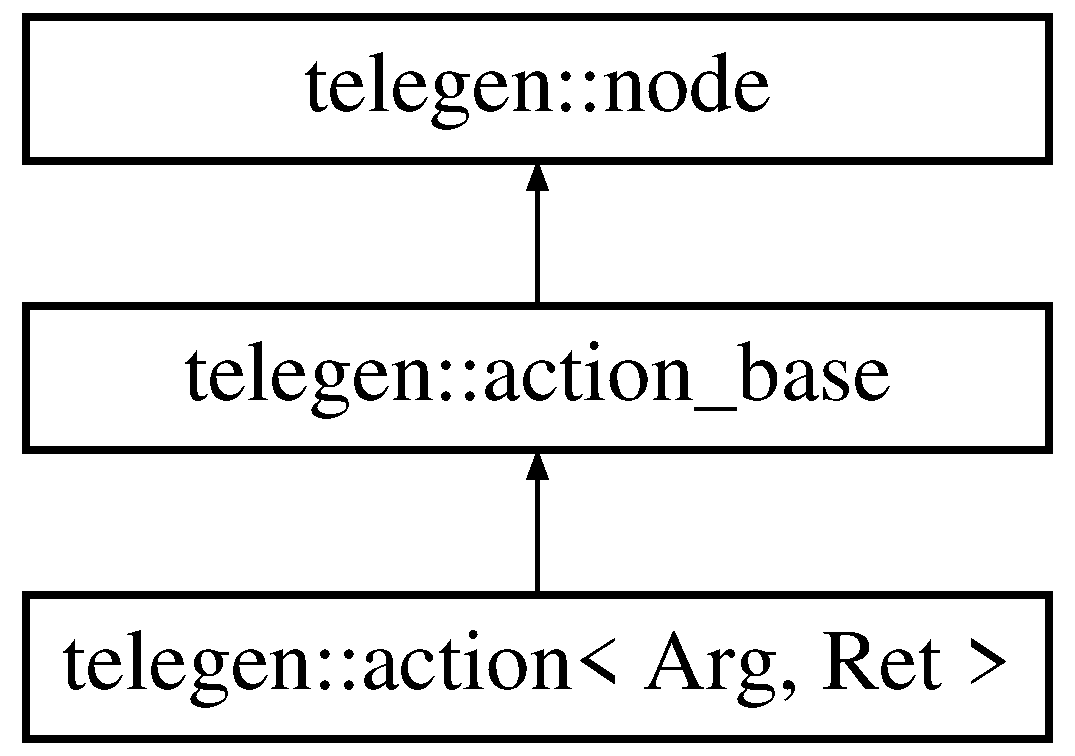
\includegraphics[height=3.000000cm]{classtelegen_1_1action}
\end{center}
\end{figure}
\subsection*{Public Member Functions}
\begin{DoxyCompactItemize}
\item 
constexpr \hyperlink{classtelegen_1_1action_abb0b9cd50183ff3125d9056585db7571}{action} (\hyperlink{classtelegen_1_1node_aae3ff0d12932c55fdc88a1743e27ea56}{id} i, const char $\ast$name, const char $\ast$pretty, const char $\ast$desc, const \hyperlink{structtelegen_1_1type__info}{type\+\_\+info}$<$ Arg $>$ $\ast$arg\+\_\+type, const \hyperlink{structtelegen_1_1type__info}{type\+\_\+info}$<$ Ret $>$ $\ast$ret\+\_\+type)
\item 
\hyperlink{namespacetelegen_a73ca2c44e7e302c2405f99a28e35acb7}{cpromise}$<$ Ret $>$ \hyperlink{classtelegen_1_1action_aebcc7f33d0abdbace3d893ef1ea07a6a}{call} (const Arg \&a)
\item 
void \hyperlink{classtelegen_1_1action_af6b57000174dc90257d52261cc9ef444}{pack} (telegraph\+\_\+\+Action $\ast$a) const
\item 
void \hyperlink{classtelegen_1_1action_a0e5686b3bf433afab1b0fda1002f95b0}{pack} (telegraph\+\_\+\+Node $\ast$n) const override
\end{DoxyCompactItemize}
\subsection*{Protected Attributes}
\begin{DoxyCompactItemize}
\item 
const \hyperlink{structtelegen_1_1type__info}{type\+\_\+info}$<$ Arg $>$ $\ast$const \hyperlink{classtelegen_1_1action_ae81a51a3863b0aa3c8f5bd6eab375681}{arg\+\_\+type\+\_\+}
\item 
const \hyperlink{structtelegen_1_1type__info}{type\+\_\+info}$<$ Ret $>$ $\ast$const \hyperlink{classtelegen_1_1action_a1e2cfbe4fec7d4c392be9d7e3d2390dc}{ret\+\_\+type\+\_\+}
\end{DoxyCompactItemize}
\subsection*{Additional Inherited Members}


\subsection{Constructor \& Destructor Documentation}
\mbox{\Hypertarget{classtelegen_1_1action_abb0b9cd50183ff3125d9056585db7571}\label{classtelegen_1_1action_abb0b9cd50183ff3125d9056585db7571}} 
\index{telegen\+::action@{telegen\+::action}!action@{action}}
\index{action@{action}!telegen\+::action@{telegen\+::action}}
\subsubsection{\texorpdfstring{action()}{action()}}
{\footnotesize\ttfamily template$<$typename Arg , typename Ret $>$ \\
constexpr \hyperlink{classtelegen_1_1action}{telegen\+::action}$<$ Arg, Ret $>$\+::\hyperlink{classtelegen_1_1action}{action} (\begin{DoxyParamCaption}\item[{\hyperlink{classtelegen_1_1node_aae3ff0d12932c55fdc88a1743e27ea56}{id}}]{i,  }\item[{const char $\ast$}]{name,  }\item[{const char $\ast$}]{pretty,  }\item[{const char $\ast$}]{desc,  }\item[{const \hyperlink{structtelegen_1_1type__info}{type\+\_\+info}$<$ Arg $>$ $\ast$}]{arg\+\_\+type,  }\item[{const \hyperlink{structtelegen_1_1type__info}{type\+\_\+info}$<$ Ret $>$ $\ast$}]{ret\+\_\+type }\end{DoxyParamCaption})\hspace{0.3cm}{\ttfamily [inline]}}



\subsection{Member Function Documentation}
\mbox{\Hypertarget{classtelegen_1_1action_aebcc7f33d0abdbace3d893ef1ea07a6a}\label{classtelegen_1_1action_aebcc7f33d0abdbace3d893ef1ea07a6a}} 
\index{telegen\+::action@{telegen\+::action}!call@{call}}
\index{call@{call}!telegen\+::action@{telegen\+::action}}
\subsubsection{\texorpdfstring{call()}{call()}}
{\footnotesize\ttfamily template$<$typename Arg , typename Ret $>$ \\
\hyperlink{namespacetelegen_a73ca2c44e7e302c2405f99a28e35acb7}{cpromise}$<$Ret$>$ \hyperlink{classtelegen_1_1action}{telegen\+::action}$<$ Arg, Ret $>$\+::call (\begin{DoxyParamCaption}\item[{const Arg \&}]{a }\end{DoxyParamCaption})\hspace{0.3cm}{\ttfamily [inline]}}

\mbox{\Hypertarget{classtelegen_1_1action_af6b57000174dc90257d52261cc9ef444}\label{classtelegen_1_1action_af6b57000174dc90257d52261cc9ef444}} 
\index{telegen\+::action@{telegen\+::action}!pack@{pack}}
\index{pack@{pack}!telegen\+::action@{telegen\+::action}}
\subsubsection{\texorpdfstring{pack()}{pack()}\hspace{0.1cm}{\footnotesize\ttfamily [1/2]}}
{\footnotesize\ttfamily template$<$typename Arg , typename Ret $>$ \\
void \hyperlink{classtelegen_1_1action}{telegen\+::action}$<$ Arg, Ret $>$\+::pack (\begin{DoxyParamCaption}\item[{telegraph\+\_\+\+Action $\ast$}]{a }\end{DoxyParamCaption}) const\hspace{0.3cm}{\ttfamily [inline]}}

\mbox{\Hypertarget{classtelegen_1_1action_a0e5686b3bf433afab1b0fda1002f95b0}\label{classtelegen_1_1action_a0e5686b3bf433afab1b0fda1002f95b0}} 
\index{telegen\+::action@{telegen\+::action}!pack@{pack}}
\index{pack@{pack}!telegen\+::action@{telegen\+::action}}
\subsubsection{\texorpdfstring{pack()}{pack()}\hspace{0.1cm}{\footnotesize\ttfamily [2/2]}}
{\footnotesize\ttfamily template$<$typename Arg , typename Ret $>$ \\
void \hyperlink{classtelegen_1_1action}{telegen\+::action}$<$ Arg, Ret $>$\+::pack (\begin{DoxyParamCaption}\item[{telegraph\+\_\+\+Node $\ast$}]{n }\end{DoxyParamCaption}) const\hspace{0.3cm}{\ttfamily [inline]}, {\ttfamily [override]}, {\ttfamily [virtual]}}



Implements \hyperlink{classtelegen_1_1node_a8b6169d62f6e7c2e301435e52442fed3}{telegen\+::node}.



\subsection{Member Data Documentation}
\mbox{\Hypertarget{classtelegen_1_1action_ae81a51a3863b0aa3c8f5bd6eab375681}\label{classtelegen_1_1action_ae81a51a3863b0aa3c8f5bd6eab375681}} 
\index{telegen\+::action@{telegen\+::action}!arg\+\_\+type\+\_\+@{arg\+\_\+type\+\_\+}}
\index{arg\+\_\+type\+\_\+@{arg\+\_\+type\+\_\+}!telegen\+::action@{telegen\+::action}}
\subsubsection{\texorpdfstring{arg\+\_\+type\+\_\+}{arg\_type\_}}
{\footnotesize\ttfamily template$<$typename Arg , typename Ret $>$ \\
const \hyperlink{structtelegen_1_1type__info}{type\+\_\+info}$<$Arg$>$$\ast$ const \hyperlink{classtelegen_1_1action}{telegen\+::action}$<$ Arg, Ret $>$\+::arg\+\_\+type\+\_\+\hspace{0.3cm}{\ttfamily [protected]}}

\mbox{\Hypertarget{classtelegen_1_1action_a1e2cfbe4fec7d4c392be9d7e3d2390dc}\label{classtelegen_1_1action_a1e2cfbe4fec7d4c392be9d7e3d2390dc}} 
\index{telegen\+::action@{telegen\+::action}!ret\+\_\+type\+\_\+@{ret\+\_\+type\+\_\+}}
\index{ret\+\_\+type\+\_\+@{ret\+\_\+type\+\_\+}!telegen\+::action@{telegen\+::action}}
\subsubsection{\texorpdfstring{ret\+\_\+type\+\_\+}{ret\_type\_}}
{\footnotesize\ttfamily template$<$typename Arg , typename Ret $>$ \\
const \hyperlink{structtelegen_1_1type__info}{type\+\_\+info}$<$Ret$>$$\ast$ const \hyperlink{classtelegen_1_1action}{telegen\+::action}$<$ Arg, Ret $>$\+::ret\+\_\+type\+\_\+\hspace{0.3cm}{\ttfamily [protected]}}



The documentation for this class was generated from the following file\+:\begin{DoxyCompactItemize}
\item 
\hyperlink{gen_2telegen_2nodes_8hpp}{gen/telegen/nodes.\+hpp}\end{DoxyCompactItemize}

\hypertarget{classtelegraph_1_1action}{}\section{telegraph\+:\+:action Class Reference}
\label{classtelegraph_1_1action}\index{telegraph\+::action@{telegraph\+::action}}


{\ttfamily \#include $<$nodes.\+hpp$>$}

Inheritance diagram for telegraph\+:\+:action\+:\begin{figure}[H]
\begin{center}
\leavevmode
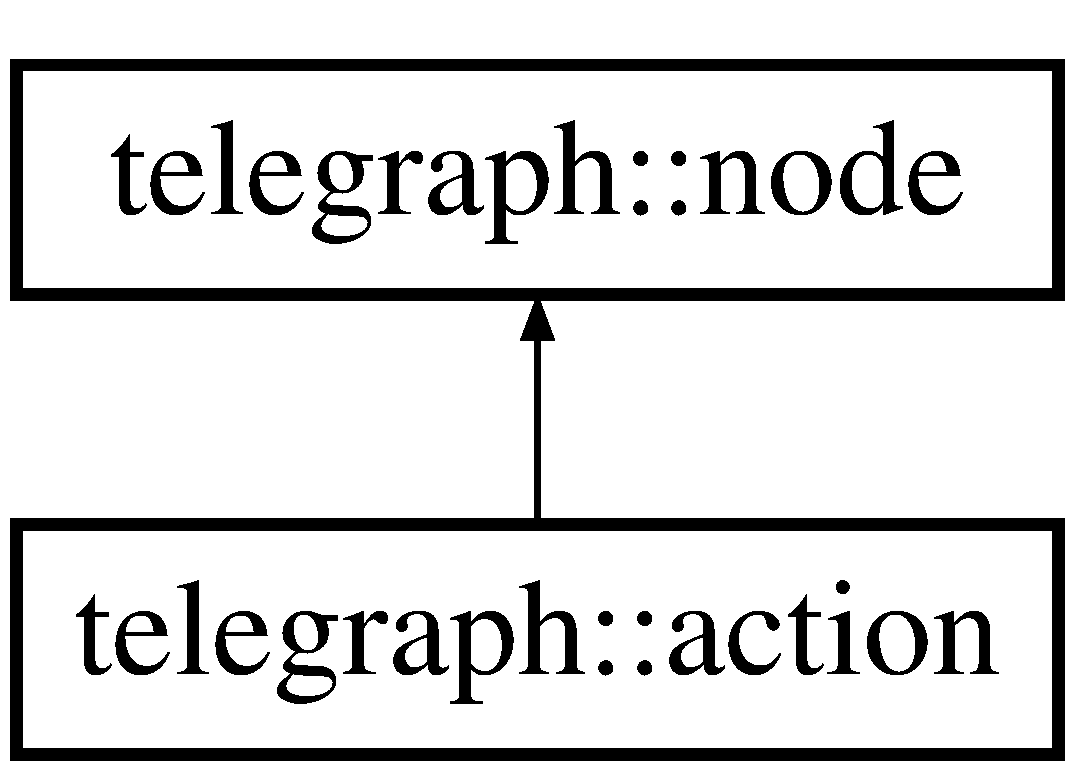
\includegraphics[height=2.000000cm]{classtelegraph_1_1action}
\end{center}
\end{figure}
\subsection*{Public Member Functions}
\begin{DoxyCompactItemize}
\item 
\hyperlink{classtelegraph_1_1action_a431cab501aaa724fc99b174804bc0024}{action} (\hyperlink{classtelegraph_1_1node_a90bc576d668ed141d5354a06aa9c8d9a}{id} i, const std\+::string\+\_\+view \&name, const std\+::string\+\_\+view \&pretty, const std\+::string\+\_\+view \&desc, const \hyperlink{classtelegraph_1_1value__type}{value\+\_\+type} \&arg\+\_\+type, const \hyperlink{classtelegraph_1_1value__type}{value\+\_\+type} \&ret\+\_\+type)
\item 
\hyperlink{classtelegraph_1_1action_a691a43a3b20d6a210dffc0f2228b8114}{action} (const \hyperlink{classtelegraph_1_1action}{action} \&a)
\item 
const \hyperlink{classtelegraph_1_1value__type}{value\+\_\+type} \& \hyperlink{classtelegraph_1_1action_a5d2e7bef5432f1246912f07296dfb4f1}{get\+\_\+arg\+\_\+type} () const
\item 
const \hyperlink{classtelegraph_1_1value__type}{value\+\_\+type} \& \hyperlink{classtelegraph_1_1action_a3d587001f7779581717b26b91564a5d8}{get\+\_\+ret\+\_\+type} () const
\item 
bool \hyperlink{classtelegraph_1_1action_a372bd4f9c1b7b4698e151448d5c28af9}{compatible\+\_\+with} (\hyperlink{classtelegraph_1_1node}{node} $\ast$other) const override
\item 
void \hyperlink{classtelegraph_1_1action_ab8b73ef00465e76e016c7f44923d4036}{pack} (Action $\ast$proto) const
\item 
virtual void \hyperlink{classtelegraph_1_1action_a849370efc692c6c4e7047e3b9c50983c}{pack} (Node $\ast$proto) const override
\item 
std\+::unique\+\_\+ptr$<$ \hyperlink{classtelegraph_1_1node}{node} $>$ \hyperlink{classtelegraph_1_1action_aa72bffae4f241be8a4366e3c7344a17b}{clone} () const override
\end{DoxyCompactItemize}
\subsection*{Static Public Member Functions}
\begin{DoxyCompactItemize}
\item 
static \hyperlink{classtelegraph_1_1action}{action} $\ast$ \hyperlink{classtelegraph_1_1action_a3eeafc85f20bfe616d7d9ea903d24267}{unpack} (const Action \&proto)
\end{DoxyCompactItemize}
\subsection*{Additional Inherited Members}


\subsection{Constructor \& Destructor Documentation}
\mbox{\Hypertarget{classtelegraph_1_1action_a431cab501aaa724fc99b174804bc0024}\label{classtelegraph_1_1action_a431cab501aaa724fc99b174804bc0024}} 
\index{telegraph\+::action@{telegraph\+::action}!action@{action}}
\index{action@{action}!telegraph\+::action@{telegraph\+::action}}
\subsubsection{\texorpdfstring{action()}{action()}\hspace{0.1cm}{\footnotesize\ttfamily [1/2]}}
{\footnotesize\ttfamily telegraph\+::action\+::action (\begin{DoxyParamCaption}\item[{\hyperlink{classtelegraph_1_1node_a90bc576d668ed141d5354a06aa9c8d9a}{id}}]{i,  }\item[{const std\+::string\+\_\+view \&}]{name,  }\item[{const std\+::string\+\_\+view \&}]{pretty,  }\item[{const std\+::string\+\_\+view \&}]{desc,  }\item[{const \hyperlink{classtelegraph_1_1value__type}{value\+\_\+type} \&}]{arg\+\_\+type,  }\item[{const \hyperlink{classtelegraph_1_1value__type}{value\+\_\+type} \&}]{ret\+\_\+type }\end{DoxyParamCaption})\hspace{0.3cm}{\ttfamily [inline]}}

\mbox{\Hypertarget{classtelegraph_1_1action_a691a43a3b20d6a210dffc0f2228b8114}\label{classtelegraph_1_1action_a691a43a3b20d6a210dffc0f2228b8114}} 
\index{telegraph\+::action@{telegraph\+::action}!action@{action}}
\index{action@{action}!telegraph\+::action@{telegraph\+::action}}
\subsubsection{\texorpdfstring{action()}{action()}\hspace{0.1cm}{\footnotesize\ttfamily [2/2]}}
{\footnotesize\ttfamily telegraph\+::action\+::action (\begin{DoxyParamCaption}\item[{const \hyperlink{classtelegraph_1_1action}{action} \&}]{a }\end{DoxyParamCaption})\hspace{0.3cm}{\ttfamily [inline]}}



\subsection{Member Function Documentation}
\mbox{\Hypertarget{classtelegraph_1_1action_aa72bffae4f241be8a4366e3c7344a17b}\label{classtelegraph_1_1action_aa72bffae4f241be8a4366e3c7344a17b}} 
\index{telegraph\+::action@{telegraph\+::action}!clone@{clone}}
\index{clone@{clone}!telegraph\+::action@{telegraph\+::action}}
\subsubsection{\texorpdfstring{clone()}{clone()}}
{\footnotesize\ttfamily std\+::unique\+\_\+ptr$<$\hyperlink{classtelegraph_1_1node}{node}$>$ telegraph\+::action\+::clone (\begin{DoxyParamCaption}{ }\end{DoxyParamCaption}) const\hspace{0.3cm}{\ttfamily [inline]}, {\ttfamily [override]}, {\ttfamily [virtual]}}



Implements \hyperlink{classtelegraph_1_1node_ae90515f4573cfa43c168cba9d542df6b}{telegraph\+::node}.

\mbox{\Hypertarget{classtelegraph_1_1action_a372bd4f9c1b7b4698e151448d5c28af9}\label{classtelegraph_1_1action_a372bd4f9c1b7b4698e151448d5c28af9}} 
\index{telegraph\+::action@{telegraph\+::action}!compatible\+\_\+with@{compatible\+\_\+with}}
\index{compatible\+\_\+with@{compatible\+\_\+with}!telegraph\+::action@{telegraph\+::action}}
\subsubsection{\texorpdfstring{compatible\+\_\+with()}{compatible\_with()}}
{\footnotesize\ttfamily bool telegraph\+::action\+::compatible\+\_\+with (\begin{DoxyParamCaption}\item[{\hyperlink{classtelegraph_1_1node}{node} $\ast$}]{other }\end{DoxyParamCaption}) const\hspace{0.3cm}{\ttfamily [override]}, {\ttfamily [virtual]}}



Implements \hyperlink{classtelegraph_1_1node_a68c4aed1434da1f0ece9089ff99ffcdb}{telegraph\+::node}.

\mbox{\Hypertarget{classtelegraph_1_1action_a5d2e7bef5432f1246912f07296dfb4f1}\label{classtelegraph_1_1action_a5d2e7bef5432f1246912f07296dfb4f1}} 
\index{telegraph\+::action@{telegraph\+::action}!get\+\_\+arg\+\_\+type@{get\+\_\+arg\+\_\+type}}
\index{get\+\_\+arg\+\_\+type@{get\+\_\+arg\+\_\+type}!telegraph\+::action@{telegraph\+::action}}
\subsubsection{\texorpdfstring{get\+\_\+arg\+\_\+type()}{get\_arg\_type()}}
{\footnotesize\ttfamily const \hyperlink{classtelegraph_1_1value__type}{value\+\_\+type}\& telegraph\+::action\+::get\+\_\+arg\+\_\+type (\begin{DoxyParamCaption}{ }\end{DoxyParamCaption}) const\hspace{0.3cm}{\ttfamily [inline]}}

\mbox{\Hypertarget{classtelegraph_1_1action_a3d587001f7779581717b26b91564a5d8}\label{classtelegraph_1_1action_a3d587001f7779581717b26b91564a5d8}} 
\index{telegraph\+::action@{telegraph\+::action}!get\+\_\+ret\+\_\+type@{get\+\_\+ret\+\_\+type}}
\index{get\+\_\+ret\+\_\+type@{get\+\_\+ret\+\_\+type}!telegraph\+::action@{telegraph\+::action}}
\subsubsection{\texorpdfstring{get\+\_\+ret\+\_\+type()}{get\_ret\_type()}}
{\footnotesize\ttfamily const \hyperlink{classtelegraph_1_1value__type}{value\+\_\+type}\& telegraph\+::action\+::get\+\_\+ret\+\_\+type (\begin{DoxyParamCaption}{ }\end{DoxyParamCaption}) const\hspace{0.3cm}{\ttfamily [inline]}}

\mbox{\Hypertarget{classtelegraph_1_1action_ab8b73ef00465e76e016c7f44923d4036}\label{classtelegraph_1_1action_ab8b73ef00465e76e016c7f44923d4036}} 
\index{telegraph\+::action@{telegraph\+::action}!pack@{pack}}
\index{pack@{pack}!telegraph\+::action@{telegraph\+::action}}
\subsubsection{\texorpdfstring{pack()}{pack()}\hspace{0.1cm}{\footnotesize\ttfamily [1/2]}}
{\footnotesize\ttfamily void telegraph\+::action\+::pack (\begin{DoxyParamCaption}\item[{Action $\ast$}]{proto }\end{DoxyParamCaption}) const}

\mbox{\Hypertarget{classtelegraph_1_1action_a849370efc692c6c4e7047e3b9c50983c}\label{classtelegraph_1_1action_a849370efc692c6c4e7047e3b9c50983c}} 
\index{telegraph\+::action@{telegraph\+::action}!pack@{pack}}
\index{pack@{pack}!telegraph\+::action@{telegraph\+::action}}
\subsubsection{\texorpdfstring{pack()}{pack()}\hspace{0.1cm}{\footnotesize\ttfamily [2/2]}}
{\footnotesize\ttfamily void telegraph\+::action\+::pack (\begin{DoxyParamCaption}\item[{Node $\ast$}]{proto }\end{DoxyParamCaption}) const\hspace{0.3cm}{\ttfamily [override]}, {\ttfamily [virtual]}}



Implements \hyperlink{classtelegraph_1_1node_a5006b21e9b83ecd52f3f953a1b828773}{telegraph\+::node}.

\mbox{\Hypertarget{classtelegraph_1_1action_a3eeafc85f20bfe616d7d9ea903d24267}\label{classtelegraph_1_1action_a3eeafc85f20bfe616d7d9ea903d24267}} 
\index{telegraph\+::action@{telegraph\+::action}!unpack@{unpack}}
\index{unpack@{unpack}!telegraph\+::action@{telegraph\+::action}}
\subsubsection{\texorpdfstring{unpack()}{unpack()}}
{\footnotesize\ttfamily \hyperlink{classtelegraph_1_1action}{action} $\ast$ telegraph\+::action\+::unpack (\begin{DoxyParamCaption}\item[{const Action \&}]{proto }\end{DoxyParamCaption})\hspace{0.3cm}{\ttfamily [static]}}



The documentation for this class was generated from the following files\+:\begin{DoxyCompactItemize}
\item 
\hyperlink{lib_2telegraph_2common_2nodes_8hpp}{lib/telegraph/common/nodes.\+hpp}\item 
\hyperlink{nodes_8cpp}{nodes.\+cpp}\end{DoxyCompactItemize}

\hypertarget{classtelegen_1_1action__base}{}\section{telegen\+:\+:action\+\_\+base Class Reference}
\label{classtelegen_1_1action__base}\index{telegen\+::action\+\_\+base@{telegen\+::action\+\_\+base}}


{\ttfamily \#include $<$nodes.\+hpp$>$}

Inheritance diagram for telegen\+:\+:action\+\_\+base\+:\begin{figure}[H]
\begin{center}
\leavevmode
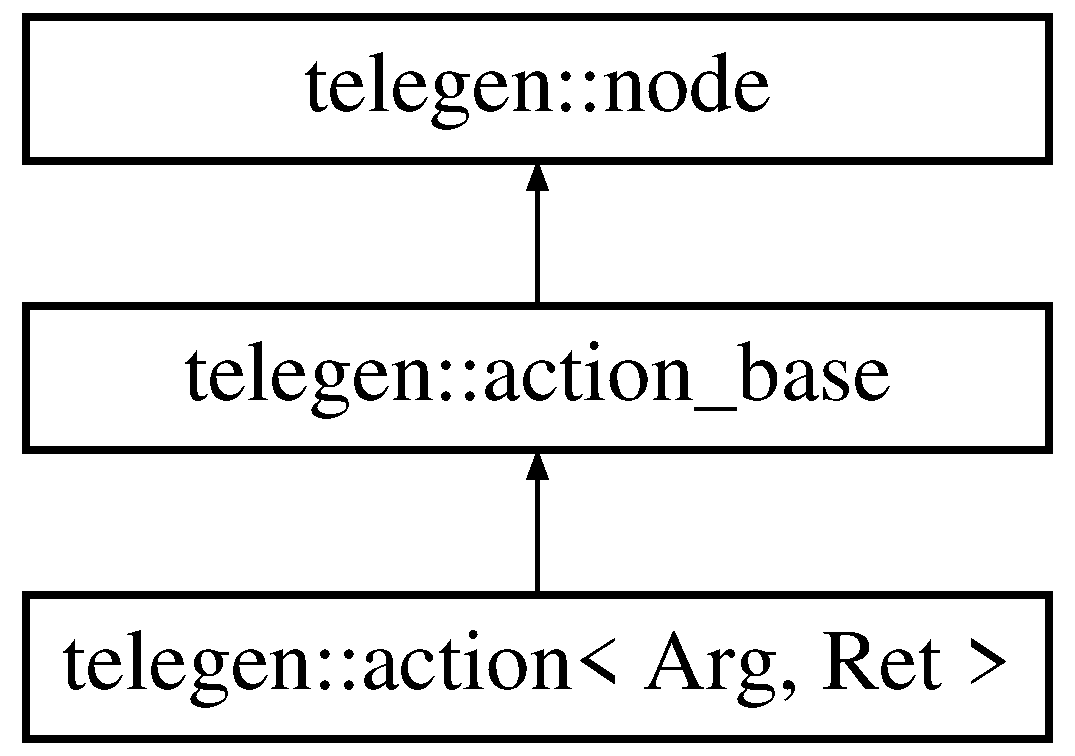
\includegraphics[height=3.000000cm]{classtelegen_1_1action__base}
\end{center}
\end{figure}
\subsection*{Public Member Functions}
\begin{DoxyCompactItemize}
\item 
constexpr \hyperlink{classtelegen_1_1action__base_a50c033aec11f3533b47fe7ad799ecb1d}{action\+\_\+base} (int32\+\_\+t \hyperlink{classtelegen_1_1node_aae3ff0d12932c55fdc88a1743e27ea56}{id}, const char $\ast$name, const char $\ast$pretty, const char $\ast$desc)
\item 
\hyperlink{namespacetelegen_a9dd802bb5d30cf96b0c616750d43ae86}{promise}$<$ \hyperlink{classtelegen_1_1value}{value} $>$ \hyperlink{classtelegen_1_1action__base_aa05f686e2a085c773bcbc8ac07da6f04}{call} (\hyperlink{classtelegen_1_1action__base}{action\+\_\+base} $\ast$a, \hyperlink{classtelegen_1_1value}{value} arg, \hyperlink{namespacetelegen_ad925de2d0a99bc43918533abf0457344}{interval} timeout)
\end{DoxyCompactItemize}
\subsection*{Additional Inherited Members}


\subsection{Constructor \& Destructor Documentation}
\mbox{\Hypertarget{classtelegen_1_1action__base_a50c033aec11f3533b47fe7ad799ecb1d}\label{classtelegen_1_1action__base_a50c033aec11f3533b47fe7ad799ecb1d}} 
\index{telegen\+::action\+\_\+base@{telegen\+::action\+\_\+base}!action\+\_\+base@{action\+\_\+base}}
\index{action\+\_\+base@{action\+\_\+base}!telegen\+::action\+\_\+base@{telegen\+::action\+\_\+base}}
\subsubsection{\texorpdfstring{action\+\_\+base()}{action\_base()}}
{\footnotesize\ttfamily constexpr telegen\+::action\+\_\+base\+::action\+\_\+base (\begin{DoxyParamCaption}\item[{int32\+\_\+t}]{id,  }\item[{const char $\ast$}]{name,  }\item[{const char $\ast$}]{pretty,  }\item[{const char $\ast$}]{desc }\end{DoxyParamCaption})\hspace{0.3cm}{\ttfamily [inline]}}



\subsection{Member Function Documentation}
\mbox{\Hypertarget{classtelegen_1_1action__base_aa05f686e2a085c773bcbc8ac07da6f04}\label{classtelegen_1_1action__base_aa05f686e2a085c773bcbc8ac07da6f04}} 
\index{telegen\+::action\+\_\+base@{telegen\+::action\+\_\+base}!call@{call}}
\index{call@{call}!telegen\+::action\+\_\+base@{telegen\+::action\+\_\+base}}
\subsubsection{\texorpdfstring{call()}{call()}}
{\footnotesize\ttfamily \hyperlink{namespacetelegen_a9dd802bb5d30cf96b0c616750d43ae86}{promise}$<$\hyperlink{classtelegen_1_1value}{value}$>$ telegen\+::action\+\_\+base\+::call (\begin{DoxyParamCaption}\item[{\hyperlink{classtelegen_1_1action__base}{action\+\_\+base} $\ast$}]{a,  }\item[{\hyperlink{classtelegen_1_1value}{value}}]{arg,  }\item[{\hyperlink{namespacetelegen_ad925de2d0a99bc43918533abf0457344}{interval}}]{timeout }\end{DoxyParamCaption})\hspace{0.3cm}{\ttfamily [inline]}}



The documentation for this class was generated from the following file\+:\begin{DoxyCompactItemize}
\item 
\hyperlink{gen_2telegen_2nodes_8hpp}{gen/telegen/nodes.\+hpp}\end{DoxyCompactItemize}

\hypertarget{classtelegen_1_1action__handler}{}\section{telegen\+:\+:action\+\_\+handler$<$ F, Arg, Ret $>$ Class Template Reference}
\label{classtelegen_1_1action__handler}\index{telegen\+::action\+\_\+handler$<$ F, Arg, Ret $>$@{telegen\+::action\+\_\+handler$<$ F, Arg, Ret $>$}}


{\ttfamily \#include $<$publisher.\+hpp$>$}

\subsection*{Public Member Functions}
\begin{DoxyCompactItemize}
\item 
\hyperlink{classtelegen_1_1action__handler_a4fd774bba853a38a28e38b4684390a87}{action\+\_\+handler} (F \&f)
\item 
\hyperlink{namespacetelegen_a9dd802bb5d30cf96b0c616750d43ae86}{promise}$<$ \hyperlink{namespacetelegen_a27c822534a5231fe1c523c81e8768afb}{subscription\+\_\+ptr} $>$ \hyperlink{classtelegen_1_1action__handler_a8a48009cf9e2893bd2801ab04465ba31}{subscribe} (\hyperlink{classtelegen_1_1variable__base}{variable\+\_\+base} $\ast$v, int32\+\_\+t min\+\_\+interval, int32\+\_\+t max\+\_\+interval)
\item 
\hyperlink{namespacetelegen_a9dd802bb5d30cf96b0c616750d43ae86}{promise}$<$ \hyperlink{classtelegen_1_1value}{value} $>$ \hyperlink{classtelegen_1_1action__handler_af74ede39066de588eb8f51b25d1b96a0}{call} (\hyperlink{classtelegen_1_1action__base}{action\+\_\+base} $\ast$a, const \hyperlink{classtelegen_1_1value}{value} \&arg)
\end{DoxyCompactItemize}


\subsection{Constructor \& Destructor Documentation}
\mbox{\Hypertarget{classtelegen_1_1action__handler_a4fd774bba853a38a28e38b4684390a87}\label{classtelegen_1_1action__handler_a4fd774bba853a38a28e38b4684390a87}} 
\index{telegen\+::action\+\_\+handler@{telegen\+::action\+\_\+handler}!action\+\_\+handler@{action\+\_\+handler}}
\index{action\+\_\+handler@{action\+\_\+handler}!telegen\+::action\+\_\+handler@{telegen\+::action\+\_\+handler}}
\subsubsection{\texorpdfstring{action\+\_\+handler()}{action\_handler()}}
{\footnotesize\ttfamily template$<$typename F , typename Arg , typename Ret $>$ \\
\hyperlink{classtelegen_1_1action__handler}{telegen\+::action\+\_\+handler}$<$ F, Arg, Ret $>$\+::\hyperlink{classtelegen_1_1action__handler}{action\+\_\+handler} (\begin{DoxyParamCaption}\item[{F \&}]{f }\end{DoxyParamCaption})\hspace{0.3cm}{\ttfamily [inline]}}



\subsection{Member Function Documentation}
\mbox{\Hypertarget{classtelegen_1_1action__handler_af74ede39066de588eb8f51b25d1b96a0}\label{classtelegen_1_1action__handler_af74ede39066de588eb8f51b25d1b96a0}} 
\index{telegen\+::action\+\_\+handler@{telegen\+::action\+\_\+handler}!call@{call}}
\index{call@{call}!telegen\+::action\+\_\+handler@{telegen\+::action\+\_\+handler}}
\subsubsection{\texorpdfstring{call()}{call()}}
{\footnotesize\ttfamily template$<$typename F , typename Arg , typename Ret $>$ \\
\hyperlink{namespacetelegen_a9dd802bb5d30cf96b0c616750d43ae86}{promise}$<$\hyperlink{classtelegen_1_1value}{value}$>$ \hyperlink{classtelegen_1_1action__handler}{telegen\+::action\+\_\+handler}$<$ F, Arg, Ret $>$\+::call (\begin{DoxyParamCaption}\item[{\hyperlink{classtelegen_1_1action__base}{action\+\_\+base} $\ast$}]{a,  }\item[{const \hyperlink{classtelegen_1_1value}{value} \&}]{arg }\end{DoxyParamCaption})\hspace{0.3cm}{\ttfamily [inline]}}

\mbox{\Hypertarget{classtelegen_1_1action__handler_a8a48009cf9e2893bd2801ab04465ba31}\label{classtelegen_1_1action__handler_a8a48009cf9e2893bd2801ab04465ba31}} 
\index{telegen\+::action\+\_\+handler@{telegen\+::action\+\_\+handler}!subscribe@{subscribe}}
\index{subscribe@{subscribe}!telegen\+::action\+\_\+handler@{telegen\+::action\+\_\+handler}}
\subsubsection{\texorpdfstring{subscribe()}{subscribe()}}
{\footnotesize\ttfamily template$<$typename F , typename Arg , typename Ret $>$ \\
\hyperlink{namespacetelegen_a9dd802bb5d30cf96b0c616750d43ae86}{promise}$<$\hyperlink{namespacetelegen_a27c822534a5231fe1c523c81e8768afb}{subscription\+\_\+ptr}$>$ \hyperlink{classtelegen_1_1action__handler}{telegen\+::action\+\_\+handler}$<$ F, Arg, Ret $>$\+::subscribe (\begin{DoxyParamCaption}\item[{\hyperlink{classtelegen_1_1variable__base}{variable\+\_\+base} $\ast$}]{v,  }\item[{int32\+\_\+t}]{min\+\_\+interval,  }\item[{int32\+\_\+t}]{max\+\_\+interval }\end{DoxyParamCaption})\hspace{0.3cm}{\ttfamily [inline]}}



The documentation for this class was generated from the following file\+:\begin{DoxyCompactItemize}
\item 
\hyperlink{gen_2telegen_2publisher_8hpp}{gen/telegen/publisher.\+hpp}\end{DoxyCompactItemize}

\hypertarget{classtelegraph_1_1adapter}{}\section{telegraph\+:\+:adapter$<$ Poll\+Func, Change\+Func, Cancel\+Func $>$ Class Template Reference}
\label{classtelegraph_1_1adapter}\index{telegraph\+::adapter$<$ Poll\+Func, Change\+Func, Cancel\+Func $>$@{telegraph\+::adapter$<$ Poll\+Func, Change\+Func, Cancel\+Func $>$}}


{\ttfamily \#include $<$adapter.\+hpp$>$}

Inheritance diagram for telegraph\+:\+:adapter$<$ Poll\+Func, Change\+Func, Cancel\+Func $>$\+:\begin{figure}[H]
\begin{center}
\leavevmode
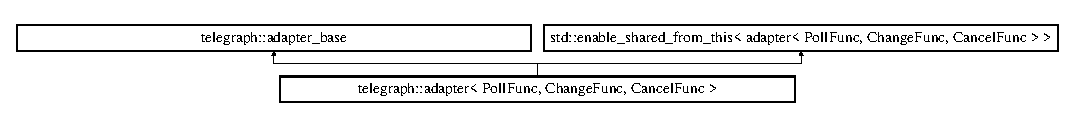
\includegraphics[height=1.154639cm]{classtelegraph_1_1adapter}
\end{center}
\end{figure}
\subsection*{Public Member Functions}
\begin{DoxyCompactItemize}
\item 
\hyperlink{classtelegraph_1_1adapter_a01578ea2a59c672e85b7c400d4b70817}{adapter} (io\+::io\+\_\+context \&ioc, \hyperlink{classtelegraph_1_1value__type}{value\+\_\+type} t, Poll\+Func poll, Change\+Func change, Cancel\+Func cancel)
\item 
void \hyperlink{classtelegraph_1_1adapter_aabfebfcdec55822a0a5228277205ab47}{update} (\hyperlink{classtelegraph_1_1value}{value} v) override
\item 
\hyperlink{namespacetelegraph_a58641aa5b1a2cbdb0431916a87069f64}{subscription\+\_\+ptr} \hyperlink{classtelegraph_1_1adapter_a0b9c93d0584817ca7dfd74f4ae38ebad}{subscribe} (\hyperlink{structboost_1_1asio_1_1yield__ctx}{io\+::yield\+\_\+ctx} \&yield, float min\+\_\+interval, float max\+\_\+interval, float timeout) override
\end{DoxyCompactItemize}
\subsection*{Friends}
\begin{DoxyCompactItemize}
\item 
class \hyperlink{classtelegraph_1_1adapter_aa1d42a83e16956670795959f328adff4}{sub}
\end{DoxyCompactItemize}


\subsection{Constructor \& Destructor Documentation}
\mbox{\Hypertarget{classtelegraph_1_1adapter_a01578ea2a59c672e85b7c400d4b70817}\label{classtelegraph_1_1adapter_a01578ea2a59c672e85b7c400d4b70817}} 
\index{telegraph\+::adapter@{telegraph\+::adapter}!adapter@{adapter}}
\index{adapter@{adapter}!telegraph\+::adapter@{telegraph\+::adapter}}
\subsubsection{\texorpdfstring{adapter()}{adapter()}}
{\footnotesize\ttfamily template$<$typename Poll\+Func , typename Change\+Func , typename Cancel\+Func $>$ \\
\hyperlink{classtelegraph_1_1adapter}{telegraph\+::adapter}$<$ Poll\+Func, Change\+Func, Cancel\+Func $>$\+::\hyperlink{classtelegraph_1_1adapter}{adapter} (\begin{DoxyParamCaption}\item[{io\+::io\+\_\+context \&}]{ioc,  }\item[{\hyperlink{classtelegraph_1_1value__type}{value\+\_\+type}}]{t,  }\item[{Poll\+Func}]{poll,  }\item[{Change\+Func}]{change,  }\item[{Cancel\+Func}]{cancel }\end{DoxyParamCaption})\hspace{0.3cm}{\ttfamily [inline]}}



\subsection{Member Function Documentation}
\mbox{\Hypertarget{classtelegraph_1_1adapter_a0b9c93d0584817ca7dfd74f4ae38ebad}\label{classtelegraph_1_1adapter_a0b9c93d0584817ca7dfd74f4ae38ebad}} 
\index{telegraph\+::adapter@{telegraph\+::adapter}!subscribe@{subscribe}}
\index{subscribe@{subscribe}!telegraph\+::adapter@{telegraph\+::adapter}}
\subsubsection{\texorpdfstring{subscribe()}{subscribe()}}
{\footnotesize\ttfamily template$<$typename Poll\+Func , typename Change\+Func , typename Cancel\+Func $>$ \\
\hyperlink{namespacetelegraph_a58641aa5b1a2cbdb0431916a87069f64}{subscription\+\_\+ptr} \hyperlink{classtelegraph_1_1adapter}{telegraph\+::adapter}$<$ Poll\+Func, Change\+Func, Cancel\+Func $>$\+::subscribe (\begin{DoxyParamCaption}\item[{\hyperlink{structboost_1_1asio_1_1yield__ctx}{io\+::yield\+\_\+ctx} \&}]{yield,  }\item[{float}]{min\+\_\+interval,  }\item[{float}]{max\+\_\+interval,  }\item[{float}]{timeout }\end{DoxyParamCaption})\hspace{0.3cm}{\ttfamily [inline]}, {\ttfamily [override]}, {\ttfamily [virtual]}}



Implements \hyperlink{classtelegraph_1_1adapter__base_a2fa110e124bc9a86c9433fe04033ff06}{telegraph\+::adapter\+\_\+base}.

\mbox{\Hypertarget{classtelegraph_1_1adapter_aabfebfcdec55822a0a5228277205ab47}\label{classtelegraph_1_1adapter_aabfebfcdec55822a0a5228277205ab47}} 
\index{telegraph\+::adapter@{telegraph\+::adapter}!update@{update}}
\index{update@{update}!telegraph\+::adapter@{telegraph\+::adapter}}
\subsubsection{\texorpdfstring{update()}{update()}}
{\footnotesize\ttfamily template$<$typename Poll\+Func , typename Change\+Func , typename Cancel\+Func $>$ \\
void \hyperlink{classtelegraph_1_1adapter}{telegraph\+::adapter}$<$ Poll\+Func, Change\+Func, Cancel\+Func $>$\+::update (\begin{DoxyParamCaption}\item[{\hyperlink{classtelegraph_1_1value}{value}}]{v }\end{DoxyParamCaption})\hspace{0.3cm}{\ttfamily [inline]}, {\ttfamily [override]}, {\ttfamily [virtual]}}



Implements \hyperlink{classtelegraph_1_1adapter__base_a3b2347f991a3c621b35f20f81419cf62}{telegraph\+::adapter\+\_\+base}.



\subsection{Friends And Related Function Documentation}
\mbox{\Hypertarget{classtelegraph_1_1adapter_aa1d42a83e16956670795959f328adff4}\label{classtelegraph_1_1adapter_aa1d42a83e16956670795959f328adff4}} 
\index{telegraph\+::adapter@{telegraph\+::adapter}!sub@{sub}}
\index{sub@{sub}!telegraph\+::adapter@{telegraph\+::adapter}}
\subsubsection{\texorpdfstring{sub}{sub}}
{\footnotesize\ttfamily template$<$typename Poll\+Func , typename Change\+Func , typename Cancel\+Func $>$ \\
friend class sub\hspace{0.3cm}{\ttfamily [friend]}}



The documentation for this class was generated from the following file\+:\begin{DoxyCompactItemize}
\item 
\hyperlink{adapter_8hpp}{adapter.\+hpp}\end{DoxyCompactItemize}

\hypertarget{classtelegraph_1_1adapter__base}{}\section{telegraph\+:\+:adapter\+\_\+base Class Reference}
\label{classtelegraph_1_1adapter__base}\index{telegraph\+::adapter\+\_\+base@{telegraph\+::adapter\+\_\+base}}


{\ttfamily \#include $<$adapter.\+hpp$>$}

Inheritance diagram for telegraph\+:\+:adapter\+\_\+base\+:\begin{figure}[H]
\begin{center}
\leavevmode
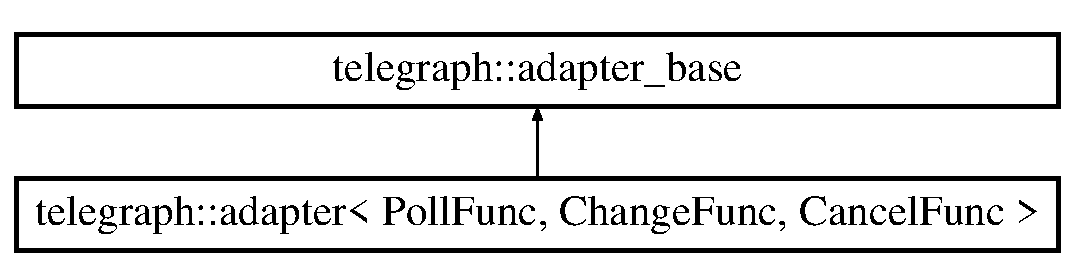
\includegraphics[height=2.000000cm]{classtelegraph_1_1adapter__base}
\end{center}
\end{figure}
\subsection*{Public Member Functions}
\begin{DoxyCompactItemize}
\item 
virtual \hyperlink{classtelegraph_1_1adapter__base_a385f1cf5e39a3cbd2c3f030caeb15451}{$\sim$adapter\+\_\+base} ()
\item 
virtual \hyperlink{namespacetelegraph_a58641aa5b1a2cbdb0431916a87069f64}{subscription\+\_\+ptr} \hyperlink{classtelegraph_1_1adapter__base_a2fa110e124bc9a86c9433fe04033ff06}{subscribe} (\hyperlink{structboost_1_1asio_1_1yield__ctx}{io\+::yield\+\_\+ctx} \&yield, float debounce, float refresh, float timeout)=0
\item 
virtual void \hyperlink{classtelegraph_1_1adapter__base_a3b2347f991a3c621b35f20f81419cf62}{update} (\hyperlink{classtelegraph_1_1value}{value} v)=0
\end{DoxyCompactItemize}


\subsection{Constructor \& Destructor Documentation}
\mbox{\Hypertarget{classtelegraph_1_1adapter__base_a385f1cf5e39a3cbd2c3f030caeb15451}\label{classtelegraph_1_1adapter__base_a385f1cf5e39a3cbd2c3f030caeb15451}} 
\index{telegraph\+::adapter\+\_\+base@{telegraph\+::adapter\+\_\+base}!````~adapter\+\_\+base@{$\sim$adapter\+\_\+base}}
\index{````~adapter\+\_\+base@{$\sim$adapter\+\_\+base}!telegraph\+::adapter\+\_\+base@{telegraph\+::adapter\+\_\+base}}
\subsubsection{\texorpdfstring{$\sim$adapter\+\_\+base()}{~adapter\_base()}}
{\footnotesize\ttfamily virtual telegraph\+::adapter\+\_\+base\+::$\sim$adapter\+\_\+base (\begin{DoxyParamCaption}{ }\end{DoxyParamCaption})\hspace{0.3cm}{\ttfamily [inline]}, {\ttfamily [virtual]}}



\subsection{Member Function Documentation}
\mbox{\Hypertarget{classtelegraph_1_1adapter__base_a2fa110e124bc9a86c9433fe04033ff06}\label{classtelegraph_1_1adapter__base_a2fa110e124bc9a86c9433fe04033ff06}} 
\index{telegraph\+::adapter\+\_\+base@{telegraph\+::adapter\+\_\+base}!subscribe@{subscribe}}
\index{subscribe@{subscribe}!telegraph\+::adapter\+\_\+base@{telegraph\+::adapter\+\_\+base}}
\subsubsection{\texorpdfstring{subscribe()}{subscribe()}}
{\footnotesize\ttfamily virtual \hyperlink{namespacetelegraph_a58641aa5b1a2cbdb0431916a87069f64}{subscription\+\_\+ptr} telegraph\+::adapter\+\_\+base\+::subscribe (\begin{DoxyParamCaption}\item[{\hyperlink{structboost_1_1asio_1_1yield__ctx}{io\+::yield\+\_\+ctx} \&}]{yield,  }\item[{float}]{debounce,  }\item[{float}]{refresh,  }\item[{float}]{timeout }\end{DoxyParamCaption})\hspace{0.3cm}{\ttfamily [pure virtual]}}



Implemented in \hyperlink{classtelegraph_1_1adapter_a0b9c93d0584817ca7dfd74f4ae38ebad}{telegraph\+::adapter$<$ Poll\+Func, Change\+Func, Cancel\+Func $>$}.

\mbox{\Hypertarget{classtelegraph_1_1adapter__base_a3b2347f991a3c621b35f20f81419cf62}\label{classtelegraph_1_1adapter__base_a3b2347f991a3c621b35f20f81419cf62}} 
\index{telegraph\+::adapter\+\_\+base@{telegraph\+::adapter\+\_\+base}!update@{update}}
\index{update@{update}!telegraph\+::adapter\+\_\+base@{telegraph\+::adapter\+\_\+base}}
\subsubsection{\texorpdfstring{update()}{update()}}
{\footnotesize\ttfamily virtual void telegraph\+::adapter\+\_\+base\+::update (\begin{DoxyParamCaption}\item[{\hyperlink{classtelegraph_1_1value}{value}}]{v }\end{DoxyParamCaption})\hspace{0.3cm}{\ttfamily [pure virtual]}}



Implemented in \hyperlink{classtelegraph_1_1adapter_aabfebfcdec55822a0a5228277205ab47}{telegraph\+::adapter$<$ Poll\+Func, Change\+Func, Cancel\+Func $>$}.



The documentation for this class was generated from the following file\+:\begin{DoxyCompactItemize}
\item 
\hyperlink{adapter_8hpp}{adapter.\+hpp}\end{DoxyCompactItemize}

\hypertarget{structstdext_1_1inplace__function__detail_1_1aligned__storage}{}\section{stdext\+:\+:inplace\+\_\+function\+\_\+detail\+:\+:aligned\+\_\+storage$<$ Cap, Align $>$ Struct Template Reference}
\label{structstdext_1_1inplace__function__detail_1_1aligned__storage}\index{stdext\+::inplace\+\_\+function\+\_\+detail\+::aligned\+\_\+storage$<$ Cap, Align $>$@{stdext\+::inplace\+\_\+function\+\_\+detail\+::aligned\+\_\+storage$<$ Cap, Align $>$}}


{\ttfamily \#include $<$inplace\+\_\+function.\+hpp$>$}

\subsection*{Public Types}
\begin{DoxyCompactItemize}
\item 
using \hyperlink{structstdext_1_1inplace__function__detail_1_1aligned__storage_a2715429b3ff736ab58dea08f28f06947}{type} = std\+::aligned\+\_\+storage\+\_\+t$<$ Cap, Align $>$
\item 
using \hyperlink{structstdext_1_1inplace__function__detail_1_1aligned__storage_a2715429b3ff736ab58dea08f28f06947}{type} = std\+::aligned\+\_\+storage\+\_\+t$<$ Cap, Align $>$
\end{DoxyCompactItemize}


\subsection{Member Typedef Documentation}
\mbox{\Hypertarget{structstdext_1_1inplace__function__detail_1_1aligned__storage_a2715429b3ff736ab58dea08f28f06947}\label{structstdext_1_1inplace__function__detail_1_1aligned__storage_a2715429b3ff736ab58dea08f28f06947}} 
\index{stdext\+::inplace\+\_\+function\+\_\+detail\+::aligned\+\_\+storage@{stdext\+::inplace\+\_\+function\+\_\+detail\+::aligned\+\_\+storage}!type@{type}}
\index{type@{type}!stdext\+::inplace\+\_\+function\+\_\+detail\+::aligned\+\_\+storage@{stdext\+::inplace\+\_\+function\+\_\+detail\+::aligned\+\_\+storage}}
\subsubsection{\texorpdfstring{type}{type}\hspace{0.1cm}{\footnotesize\ttfamily [1/2]}}
{\footnotesize\ttfamily template$<$size\+\_\+t Cap, size\+\_\+t Align = alignof(aligned\+\_\+storage\+\_\+helper$<$\+Cap$>$)$>$ \\
using \hyperlink{structstdext_1_1inplace__function__detail_1_1aligned__storage}{stdext\+::inplace\+\_\+function\+\_\+detail\+::aligned\+\_\+storage}$<$ Cap, Align $>$\+::\hyperlink{structstdext_1_1inplace__function__detail_1_1aligned__storage_a2715429b3ff736ab58dea08f28f06947}{type} =  std\+::aligned\+\_\+storage\+\_\+t$<$Cap, Align$>$}

\mbox{\Hypertarget{structstdext_1_1inplace__function__detail_1_1aligned__storage_a2715429b3ff736ab58dea08f28f06947}\label{structstdext_1_1inplace__function__detail_1_1aligned__storage_a2715429b3ff736ab58dea08f28f06947}} 
\index{stdext\+::inplace\+\_\+function\+\_\+detail\+::aligned\+\_\+storage@{stdext\+::inplace\+\_\+function\+\_\+detail\+::aligned\+\_\+storage}!type@{type}}
\index{type@{type}!stdext\+::inplace\+\_\+function\+\_\+detail\+::aligned\+\_\+storage@{stdext\+::inplace\+\_\+function\+\_\+detail\+::aligned\+\_\+storage}}
\subsubsection{\texorpdfstring{type}{type}\hspace{0.1cm}{\footnotesize\ttfamily [2/2]}}
{\footnotesize\ttfamily template$<$size\+\_\+t Cap, size\+\_\+t Align = alignof(aligned\+\_\+storage\+\_\+helper$<$\+Cap$>$)$>$ \\
using \hyperlink{structstdext_1_1inplace__function__detail_1_1aligned__storage}{stdext\+::inplace\+\_\+function\+\_\+detail\+::aligned\+\_\+storage}$<$ Cap, Align $>$\+::\hyperlink{structstdext_1_1inplace__function__detail_1_1aligned__storage_a2715429b3ff736ab58dea08f28f06947}{type} =  std\+::aligned\+\_\+storage\+\_\+t$<$Cap, Align$>$}



The documentation for this struct was generated from the following file\+:\begin{DoxyCompactItemize}
\item 
\hyperlink{gen_2telegen_2inplace__function_8hpp}{gen/telegen/inplace\+\_\+function.\+hpp}\end{DoxyCompactItemize}

\hypertarget{unionstdext_1_1inplace__function__detail_1_1aligned__storage__helper}{}\section{stdext\+:\+:inplace\+\_\+function\+\_\+detail\+:\+:aligned\+\_\+storage\+\_\+helper$<$ Cap $>$ Union Template Reference}
\label{unionstdext_1_1inplace__function__detail_1_1aligned__storage__helper}\index{stdext\+::inplace\+\_\+function\+\_\+detail\+::aligned\+\_\+storage\+\_\+helper$<$ Cap $>$@{stdext\+::inplace\+\_\+function\+\_\+detail\+::aligned\+\_\+storage\+\_\+helper$<$ Cap $>$}}


{\ttfamily \#include $<$inplace\+\_\+function.\+hpp$>$}

\subsection*{Classes}
\begin{DoxyCompactItemize}
\item 
struct \hyperlink{structstdext_1_1inplace__function__detail_1_1aligned__storage__helper_1_1double1}{double1}
\item 
struct \hyperlink{structstdext_1_1inplace__function__detail_1_1aligned__storage__helper_1_1double4}{double4}
\end{DoxyCompactItemize}
\subsection*{Public Types}
\begin{DoxyCompactItemize}
\item 
{\footnotesize template$<$class T $>$ }\\using \hyperlink{unionstdext_1_1inplace__function__detail_1_1aligned__storage__helper_a8265d2d65d57b5e7de088f8b6fc02370}{maybe} = std\+::conditional\+\_\+t$<$(Cap $>$=sizeof(T)), T, char $>$
\item 
{\footnotesize template$<$class T $>$ }\\using \hyperlink{unionstdext_1_1inplace__function__detail_1_1aligned__storage__helper_a8265d2d65d57b5e7de088f8b6fc02370}{maybe} = std\+::conditional\+\_\+t$<$(Cap $>$=sizeof(T)), T, char $>$
\end{DoxyCompactItemize}
\subsection*{Public Attributes}
\begin{DoxyCompactItemize}
\item 
char \hyperlink{unionstdext_1_1inplace__function__detail_1_1aligned__storage__helper_ae41b7c85be0b0ea99933e3c615864df0}{real\+\_\+data} \mbox{[}Cap\mbox{]}
\item 
\hyperlink{unionstdext_1_1inplace__function__detail_1_1aligned__storage__helper_a8265d2d65d57b5e7de088f8b6fc02370}{maybe}$<$ int $>$ \hyperlink{unionstdext_1_1inplace__function__detail_1_1aligned__storage__helper_af004f7336a4fed40e87fe79d09a9c72f}{a}
\item 
\hyperlink{unionstdext_1_1inplace__function__detail_1_1aligned__storage__helper_a8265d2d65d57b5e7de088f8b6fc02370}{maybe}$<$ long $>$ \hyperlink{unionstdext_1_1inplace__function__detail_1_1aligned__storage__helper_a032cd3fd7df6feed8f515f61fd91d345}{b}
\item 
\hyperlink{unionstdext_1_1inplace__function__detail_1_1aligned__storage__helper_a8265d2d65d57b5e7de088f8b6fc02370}{maybe}$<$ long long $>$ \hyperlink{unionstdext_1_1inplace__function__detail_1_1aligned__storage__helper_a7bcac46d1d7574edfe5f59838ec0e4ff}{c}
\item 
\hyperlink{unionstdext_1_1inplace__function__detail_1_1aligned__storage__helper_a8265d2d65d57b5e7de088f8b6fc02370}{maybe}$<$ void $\ast$ $>$ \hyperlink{unionstdext_1_1inplace__function__detail_1_1aligned__storage__helper_a4184b86861e804b51e0e4e2b784585ea}{d}
\item 
\hyperlink{unionstdext_1_1inplace__function__detail_1_1aligned__storage__helper_a8265d2d65d57b5e7de088f8b6fc02370}{maybe}$<$ void($\ast$)()$>$ \hyperlink{unionstdext_1_1inplace__function__detail_1_1aligned__storage__helper_abd0e5c31a14b58c138889d7b59a2bea7}{e}
\item 
\hyperlink{unionstdext_1_1inplace__function__detail_1_1aligned__storage__helper_a8265d2d65d57b5e7de088f8b6fc02370}{maybe}$<$ \hyperlink{structstdext_1_1inplace__function__detail_1_1aligned__storage__helper_1_1double1}{double1} $>$ \hyperlink{unionstdext_1_1inplace__function__detail_1_1aligned__storage__helper_a3d89d23804162fcae83e24dcaf6a5acd}{f}
\item 
\hyperlink{unionstdext_1_1inplace__function__detail_1_1aligned__storage__helper_a8265d2d65d57b5e7de088f8b6fc02370}{maybe}$<$ \hyperlink{structstdext_1_1inplace__function__detail_1_1aligned__storage__helper_1_1double4}{double4} $>$ \hyperlink{unionstdext_1_1inplace__function__detail_1_1aligned__storage__helper_a3ec253d4296818e85bb04c048b321bf8}{g}
\item 
\hyperlink{unionstdext_1_1inplace__function__detail_1_1aligned__storage__helper_a8265d2d65d57b5e7de088f8b6fc02370}{maybe}$<$ long double $>$ \hyperlink{unionstdext_1_1inplace__function__detail_1_1aligned__storage__helper_a790aee0f127912bcebca554a2cc75395}{h}
\end{DoxyCompactItemize}


\subsection{Member Typedef Documentation}
\mbox{\Hypertarget{unionstdext_1_1inplace__function__detail_1_1aligned__storage__helper_a8265d2d65d57b5e7de088f8b6fc02370}\label{unionstdext_1_1inplace__function__detail_1_1aligned__storage__helper_a8265d2d65d57b5e7de088f8b6fc02370}} 
\index{stdext\+::inplace\+\_\+function\+\_\+detail\+::aligned\+\_\+storage\+\_\+helper@{stdext\+::inplace\+\_\+function\+\_\+detail\+::aligned\+\_\+storage\+\_\+helper}!maybe@{maybe}}
\index{maybe@{maybe}!stdext\+::inplace\+\_\+function\+\_\+detail\+::aligned\+\_\+storage\+\_\+helper@{stdext\+::inplace\+\_\+function\+\_\+detail\+::aligned\+\_\+storage\+\_\+helper}}
\subsubsection{\texorpdfstring{maybe}{maybe}\hspace{0.1cm}{\footnotesize\ttfamily [1/2]}}
{\footnotesize\ttfamily template$<$size\+\_\+t Cap$>$ \\
template$<$class T $>$ \\
using \hyperlink{unionstdext_1_1inplace__function__detail_1_1aligned__storage__helper}{stdext\+::inplace\+\_\+function\+\_\+detail\+::aligned\+\_\+storage\+\_\+helper}$<$ Cap $>$\+::\hyperlink{unionstdext_1_1inplace__function__detail_1_1aligned__storage__helper_a8265d2d65d57b5e7de088f8b6fc02370}{maybe} =  std\+::conditional\+\_\+t$<$(Cap $>$= sizeof(T)), T, char$>$}

\mbox{\Hypertarget{unionstdext_1_1inplace__function__detail_1_1aligned__storage__helper_a8265d2d65d57b5e7de088f8b6fc02370}\label{unionstdext_1_1inplace__function__detail_1_1aligned__storage__helper_a8265d2d65d57b5e7de088f8b6fc02370}} 
\index{stdext\+::inplace\+\_\+function\+\_\+detail\+::aligned\+\_\+storage\+\_\+helper@{stdext\+::inplace\+\_\+function\+\_\+detail\+::aligned\+\_\+storage\+\_\+helper}!maybe@{maybe}}
\index{maybe@{maybe}!stdext\+::inplace\+\_\+function\+\_\+detail\+::aligned\+\_\+storage\+\_\+helper@{stdext\+::inplace\+\_\+function\+\_\+detail\+::aligned\+\_\+storage\+\_\+helper}}
\subsubsection{\texorpdfstring{maybe}{maybe}\hspace{0.1cm}{\footnotesize\ttfamily [2/2]}}
{\footnotesize\ttfamily template$<$size\+\_\+t Cap$>$ \\
template$<$class T $>$ \\
using \hyperlink{unionstdext_1_1inplace__function__detail_1_1aligned__storage__helper}{stdext\+::inplace\+\_\+function\+\_\+detail\+::aligned\+\_\+storage\+\_\+helper}$<$ Cap $>$\+::\hyperlink{unionstdext_1_1inplace__function__detail_1_1aligned__storage__helper_a8265d2d65d57b5e7de088f8b6fc02370}{maybe} =  std\+::conditional\+\_\+t$<$(Cap $>$= sizeof(T)), T, char$>$}



\subsection{Member Data Documentation}
\mbox{\Hypertarget{unionstdext_1_1inplace__function__detail_1_1aligned__storage__helper_af004f7336a4fed40e87fe79d09a9c72f}\label{unionstdext_1_1inplace__function__detail_1_1aligned__storage__helper_af004f7336a4fed40e87fe79d09a9c72f}} 
\index{stdext\+::inplace\+\_\+function\+\_\+detail\+::aligned\+\_\+storage\+\_\+helper@{stdext\+::inplace\+\_\+function\+\_\+detail\+::aligned\+\_\+storage\+\_\+helper}!a@{a}}
\index{a@{a}!stdext\+::inplace\+\_\+function\+\_\+detail\+::aligned\+\_\+storage\+\_\+helper@{stdext\+::inplace\+\_\+function\+\_\+detail\+::aligned\+\_\+storage\+\_\+helper}}
\subsubsection{\texorpdfstring{a}{a}}
{\footnotesize\ttfamily template$<$size\+\_\+t Cap$>$ \\
\hyperlink{unionstdext_1_1inplace__function__detail_1_1aligned__storage__helper_a8265d2d65d57b5e7de088f8b6fc02370}{maybe}$<$ int $>$ \hyperlink{unionstdext_1_1inplace__function__detail_1_1aligned__storage__helper}{stdext\+::inplace\+\_\+function\+\_\+detail\+::aligned\+\_\+storage\+\_\+helper}$<$ Cap $>$\+::a}

\mbox{\Hypertarget{unionstdext_1_1inplace__function__detail_1_1aligned__storage__helper_a032cd3fd7df6feed8f515f61fd91d345}\label{unionstdext_1_1inplace__function__detail_1_1aligned__storage__helper_a032cd3fd7df6feed8f515f61fd91d345}} 
\index{stdext\+::inplace\+\_\+function\+\_\+detail\+::aligned\+\_\+storage\+\_\+helper@{stdext\+::inplace\+\_\+function\+\_\+detail\+::aligned\+\_\+storage\+\_\+helper}!b@{b}}
\index{b@{b}!stdext\+::inplace\+\_\+function\+\_\+detail\+::aligned\+\_\+storage\+\_\+helper@{stdext\+::inplace\+\_\+function\+\_\+detail\+::aligned\+\_\+storage\+\_\+helper}}
\subsubsection{\texorpdfstring{b}{b}}
{\footnotesize\ttfamily template$<$size\+\_\+t Cap$>$ \\
\hyperlink{unionstdext_1_1inplace__function__detail_1_1aligned__storage__helper_a8265d2d65d57b5e7de088f8b6fc02370}{maybe}$<$ long $>$ \hyperlink{unionstdext_1_1inplace__function__detail_1_1aligned__storage__helper}{stdext\+::inplace\+\_\+function\+\_\+detail\+::aligned\+\_\+storage\+\_\+helper}$<$ Cap $>$\+::b}

\mbox{\Hypertarget{unionstdext_1_1inplace__function__detail_1_1aligned__storage__helper_a7bcac46d1d7574edfe5f59838ec0e4ff}\label{unionstdext_1_1inplace__function__detail_1_1aligned__storage__helper_a7bcac46d1d7574edfe5f59838ec0e4ff}} 
\index{stdext\+::inplace\+\_\+function\+\_\+detail\+::aligned\+\_\+storage\+\_\+helper@{stdext\+::inplace\+\_\+function\+\_\+detail\+::aligned\+\_\+storage\+\_\+helper}!c@{c}}
\index{c@{c}!stdext\+::inplace\+\_\+function\+\_\+detail\+::aligned\+\_\+storage\+\_\+helper@{stdext\+::inplace\+\_\+function\+\_\+detail\+::aligned\+\_\+storage\+\_\+helper}}
\subsubsection{\texorpdfstring{c}{c}}
{\footnotesize\ttfamily template$<$size\+\_\+t Cap$>$ \\
\hyperlink{unionstdext_1_1inplace__function__detail_1_1aligned__storage__helper_a8265d2d65d57b5e7de088f8b6fc02370}{maybe}$<$ long long $>$ \hyperlink{unionstdext_1_1inplace__function__detail_1_1aligned__storage__helper}{stdext\+::inplace\+\_\+function\+\_\+detail\+::aligned\+\_\+storage\+\_\+helper}$<$ Cap $>$\+::c}

\mbox{\Hypertarget{unionstdext_1_1inplace__function__detail_1_1aligned__storage__helper_a4184b86861e804b51e0e4e2b784585ea}\label{unionstdext_1_1inplace__function__detail_1_1aligned__storage__helper_a4184b86861e804b51e0e4e2b784585ea}} 
\index{stdext\+::inplace\+\_\+function\+\_\+detail\+::aligned\+\_\+storage\+\_\+helper@{stdext\+::inplace\+\_\+function\+\_\+detail\+::aligned\+\_\+storage\+\_\+helper}!d@{d}}
\index{d@{d}!stdext\+::inplace\+\_\+function\+\_\+detail\+::aligned\+\_\+storage\+\_\+helper@{stdext\+::inplace\+\_\+function\+\_\+detail\+::aligned\+\_\+storage\+\_\+helper}}
\subsubsection{\texorpdfstring{d}{d}}
{\footnotesize\ttfamily template$<$size\+\_\+t Cap$>$ \\
\hyperlink{unionstdext_1_1inplace__function__detail_1_1aligned__storage__helper_a8265d2d65d57b5e7de088f8b6fc02370}{maybe}$<$ void $\ast$ $>$ \hyperlink{unionstdext_1_1inplace__function__detail_1_1aligned__storage__helper}{stdext\+::inplace\+\_\+function\+\_\+detail\+::aligned\+\_\+storage\+\_\+helper}$<$ Cap $>$\+::d}

\mbox{\Hypertarget{unionstdext_1_1inplace__function__detail_1_1aligned__storage__helper_abd0e5c31a14b58c138889d7b59a2bea7}\label{unionstdext_1_1inplace__function__detail_1_1aligned__storage__helper_abd0e5c31a14b58c138889d7b59a2bea7}} 
\index{stdext\+::inplace\+\_\+function\+\_\+detail\+::aligned\+\_\+storage\+\_\+helper@{stdext\+::inplace\+\_\+function\+\_\+detail\+::aligned\+\_\+storage\+\_\+helper}!e@{e}}
\index{e@{e}!stdext\+::inplace\+\_\+function\+\_\+detail\+::aligned\+\_\+storage\+\_\+helper@{stdext\+::inplace\+\_\+function\+\_\+detail\+::aligned\+\_\+storage\+\_\+helper}}
\subsubsection{\texorpdfstring{e}{e}}
{\footnotesize\ttfamily template$<$size\+\_\+t Cap$>$ \\
\hyperlink{unionstdext_1_1inplace__function__detail_1_1aligned__storage__helper_a8265d2d65d57b5e7de088f8b6fc02370}{maybe}$<$ void($\ast$)()$>$ \hyperlink{unionstdext_1_1inplace__function__detail_1_1aligned__storage__helper}{stdext\+::inplace\+\_\+function\+\_\+detail\+::aligned\+\_\+storage\+\_\+helper}$<$ Cap $>$\+::e}

\mbox{\Hypertarget{unionstdext_1_1inplace__function__detail_1_1aligned__storage__helper_a3d89d23804162fcae83e24dcaf6a5acd}\label{unionstdext_1_1inplace__function__detail_1_1aligned__storage__helper_a3d89d23804162fcae83e24dcaf6a5acd}} 
\index{stdext\+::inplace\+\_\+function\+\_\+detail\+::aligned\+\_\+storage\+\_\+helper@{stdext\+::inplace\+\_\+function\+\_\+detail\+::aligned\+\_\+storage\+\_\+helper}!f@{f}}
\index{f@{f}!stdext\+::inplace\+\_\+function\+\_\+detail\+::aligned\+\_\+storage\+\_\+helper@{stdext\+::inplace\+\_\+function\+\_\+detail\+::aligned\+\_\+storage\+\_\+helper}}
\subsubsection{\texorpdfstring{f}{f}}
{\footnotesize\ttfamily template$<$size\+\_\+t Cap$>$ \\
\hyperlink{unionstdext_1_1inplace__function__detail_1_1aligned__storage__helper_a8265d2d65d57b5e7de088f8b6fc02370}{maybe}$<$ \hyperlink{structstdext_1_1inplace__function__detail_1_1aligned__storage__helper_1_1double1}{double1} $>$ \hyperlink{unionstdext_1_1inplace__function__detail_1_1aligned__storage__helper}{stdext\+::inplace\+\_\+function\+\_\+detail\+::aligned\+\_\+storage\+\_\+helper}$<$ Cap $>$\+::f}

\mbox{\Hypertarget{unionstdext_1_1inplace__function__detail_1_1aligned__storage__helper_a3ec253d4296818e85bb04c048b321bf8}\label{unionstdext_1_1inplace__function__detail_1_1aligned__storage__helper_a3ec253d4296818e85bb04c048b321bf8}} 
\index{stdext\+::inplace\+\_\+function\+\_\+detail\+::aligned\+\_\+storage\+\_\+helper@{stdext\+::inplace\+\_\+function\+\_\+detail\+::aligned\+\_\+storage\+\_\+helper}!g@{g}}
\index{g@{g}!stdext\+::inplace\+\_\+function\+\_\+detail\+::aligned\+\_\+storage\+\_\+helper@{stdext\+::inplace\+\_\+function\+\_\+detail\+::aligned\+\_\+storage\+\_\+helper}}
\subsubsection{\texorpdfstring{g}{g}}
{\footnotesize\ttfamily template$<$size\+\_\+t Cap$>$ \\
\hyperlink{unionstdext_1_1inplace__function__detail_1_1aligned__storage__helper_a8265d2d65d57b5e7de088f8b6fc02370}{maybe}$<$ \hyperlink{structstdext_1_1inplace__function__detail_1_1aligned__storage__helper_1_1double4}{double4} $>$ \hyperlink{unionstdext_1_1inplace__function__detail_1_1aligned__storage__helper}{stdext\+::inplace\+\_\+function\+\_\+detail\+::aligned\+\_\+storage\+\_\+helper}$<$ Cap $>$\+::g}

\mbox{\Hypertarget{unionstdext_1_1inplace__function__detail_1_1aligned__storage__helper_a790aee0f127912bcebca554a2cc75395}\label{unionstdext_1_1inplace__function__detail_1_1aligned__storage__helper_a790aee0f127912bcebca554a2cc75395}} 
\index{stdext\+::inplace\+\_\+function\+\_\+detail\+::aligned\+\_\+storage\+\_\+helper@{stdext\+::inplace\+\_\+function\+\_\+detail\+::aligned\+\_\+storage\+\_\+helper}!h@{h}}
\index{h@{h}!stdext\+::inplace\+\_\+function\+\_\+detail\+::aligned\+\_\+storage\+\_\+helper@{stdext\+::inplace\+\_\+function\+\_\+detail\+::aligned\+\_\+storage\+\_\+helper}}
\subsubsection{\texorpdfstring{h}{h}}
{\footnotesize\ttfamily template$<$size\+\_\+t Cap$>$ \\
\hyperlink{unionstdext_1_1inplace__function__detail_1_1aligned__storage__helper_a8265d2d65d57b5e7de088f8b6fc02370}{maybe}$<$ long double $>$ \hyperlink{unionstdext_1_1inplace__function__detail_1_1aligned__storage__helper}{stdext\+::inplace\+\_\+function\+\_\+detail\+::aligned\+\_\+storage\+\_\+helper}$<$ Cap $>$\+::h}

\mbox{\Hypertarget{unionstdext_1_1inplace__function__detail_1_1aligned__storage__helper_ae41b7c85be0b0ea99933e3c615864df0}\label{unionstdext_1_1inplace__function__detail_1_1aligned__storage__helper_ae41b7c85be0b0ea99933e3c615864df0}} 
\index{stdext\+::inplace\+\_\+function\+\_\+detail\+::aligned\+\_\+storage\+\_\+helper@{stdext\+::inplace\+\_\+function\+\_\+detail\+::aligned\+\_\+storage\+\_\+helper}!real\+\_\+data@{real\+\_\+data}}
\index{real\+\_\+data@{real\+\_\+data}!stdext\+::inplace\+\_\+function\+\_\+detail\+::aligned\+\_\+storage\+\_\+helper@{stdext\+::inplace\+\_\+function\+\_\+detail\+::aligned\+\_\+storage\+\_\+helper}}
\subsubsection{\texorpdfstring{real\+\_\+data}{real\_data}}
{\footnotesize\ttfamily template$<$size\+\_\+t Cap$>$ \\
char \hyperlink{unionstdext_1_1inplace__function__detail_1_1aligned__storage__helper}{stdext\+::inplace\+\_\+function\+\_\+detail\+::aligned\+\_\+storage\+\_\+helper}$<$ Cap $>$\+::real\+\_\+data}



The documentation for this union was generated from the following file\+:\begin{DoxyCompactItemize}
\item 
\hyperlink{gen_2telegen_2inplace__function_8hpp}{gen/telegen/inplace\+\_\+function.\+hpp}\end{DoxyCompactItemize}

\hypertarget{classtelegraph_1_1bad__type__error}{}\section{telegraph\+:\+:bad\+\_\+type\+\_\+error Class Reference}
\label{classtelegraph_1_1bad__type__error}\index{telegraph\+::bad\+\_\+type\+\_\+error@{telegraph\+::bad\+\_\+type\+\_\+error}}


{\ttfamily \#include $<$errors.\+hpp$>$}

Inheritance diagram for telegraph\+:\+:bad\+\_\+type\+\_\+error\+:\begin{figure}[H]
\begin{center}
\leavevmode
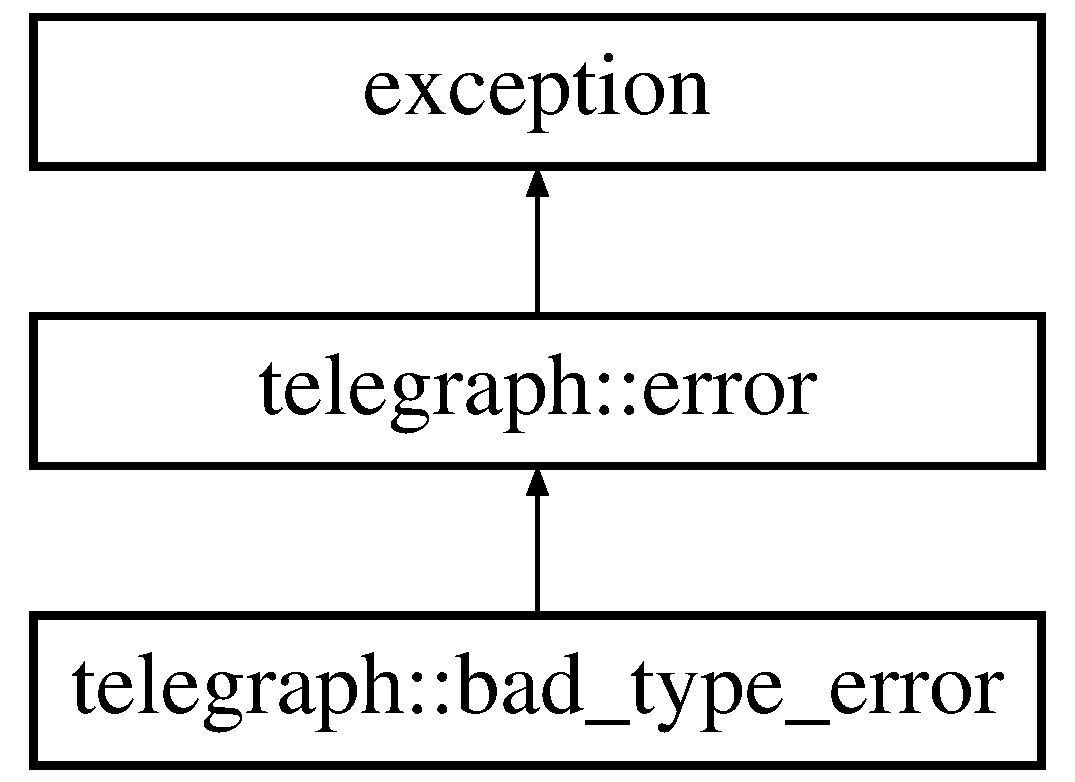
\includegraphics[height=3.000000cm]{classtelegraph_1_1bad__type__error}
\end{center}
\end{figure}
\subsection*{Public Member Functions}
\begin{DoxyCompactItemize}
\item 
\hyperlink{classtelegraph_1_1bad__type__error_a76c0b081a2d07635a4c587f987fbad42}{bad\+\_\+type\+\_\+error} (const std\+::string\+\_\+view \&m)
\end{DoxyCompactItemize}


\subsection{Constructor \& Destructor Documentation}
\mbox{\Hypertarget{classtelegraph_1_1bad__type__error_a76c0b081a2d07635a4c587f987fbad42}\label{classtelegraph_1_1bad__type__error_a76c0b081a2d07635a4c587f987fbad42}} 
\index{telegraph\+::bad\+\_\+type\+\_\+error@{telegraph\+::bad\+\_\+type\+\_\+error}!bad\+\_\+type\+\_\+error@{bad\+\_\+type\+\_\+error}}
\index{bad\+\_\+type\+\_\+error@{bad\+\_\+type\+\_\+error}!telegraph\+::bad\+\_\+type\+\_\+error@{telegraph\+::bad\+\_\+type\+\_\+error}}
\subsubsection{\texorpdfstring{bad\+\_\+type\+\_\+error()}{bad\_type\_error()}}
{\footnotesize\ttfamily telegraph\+::bad\+\_\+type\+\_\+error\+::bad\+\_\+type\+\_\+error (\begin{DoxyParamCaption}\item[{const std\+::string\+\_\+view \&}]{m }\end{DoxyParamCaption})\hspace{0.3cm}{\ttfamily [inline]}}



The documentation for this class was generated from the following file\+:\begin{DoxyCompactItemize}
\item 
\hyperlink{errors_8hpp}{errors.\+hpp}\end{DoxyCompactItemize}

\hypertarget{classtelegen_1_1basic__promise}{}\section{telegen\+:\+:basic\+\_\+promise$<$ Cap, T $>$ Class Template Reference}
\label{classtelegen_1_1basic__promise}\index{telegen\+::basic\+\_\+promise$<$ Cap, T $>$@{telegen\+::basic\+\_\+promise$<$ Cap, T $>$}}


{\ttfamily \#include $<$promise.\+hpp$>$}

Inheritance diagram for telegen\+:\+:basic\+\_\+promise$<$ Cap, T $>$\+:\begin{figure}[H]
\begin{center}
\leavevmode
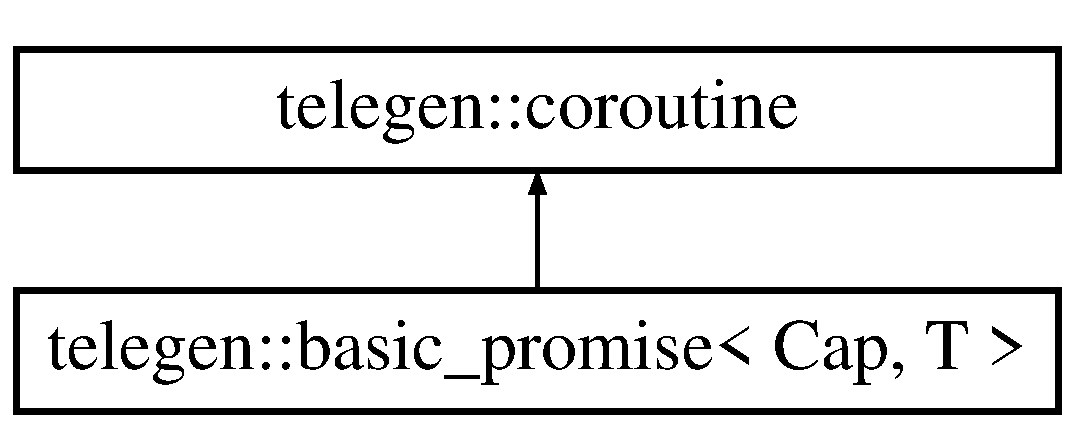
\includegraphics[height=2.000000cm]{classtelegen_1_1basic__promise}
\end{center}
\end{figure}
\subsection*{Public Types}
\begin{DoxyCompactItemize}
\item 
using \hyperlink{classtelegen_1_1basic__promise_a41bba6927e718eed58a7e6e91db6f6d3}{func} = typename \hyperlink{classtelegen_1_1basic__promise__completer}{basic\+\_\+promise\+\_\+completer}$<$ Cap, T... $>$\+::\hyperlink{classtelegen_1_1basic__promise_a41bba6927e718eed58a7e6e91db6f6d3}{func}
\end{DoxyCompactItemize}
\subsection*{Public Member Functions}
\begin{DoxyCompactItemize}
\item 
\hyperlink{classtelegen_1_1basic__promise_a2fc82b832b36b925b1c1fd42dd37cf40}{basic\+\_\+promise} (\hyperlink{namespacetelegen_a51e8b7480c7247182e2c6ca35e2c7504}{promise\+\_\+status} s)
\item 
\hyperlink{classtelegen_1_1basic__promise_a836472488ebd1d41cf9070420903848c}{basic\+\_\+promise} (T \&\&... val)
\item 
\hyperlink{classtelegen_1_1basic__promise_a6ac5ae1e598293c22075b8bd9b87bc6b}{basic\+\_\+promise} (\hyperlink{classtelegen_1_1basic__promise__completer}{basic\+\_\+promise\+\_\+completer}$<$ Cap, T... $>$ $\ast$obj)
\item 
\hyperlink{classtelegen_1_1basic__promise_a0c1f0ae0a200d107a8ab62afb48e6ffd}{basic\+\_\+promise} (\hyperlink{classtelegen_1_1basic__promise}{basic\+\_\+promise}$<$ Cap, T... $>$ \&\&p)
\item 
\hyperlink{classtelegen_1_1basic__promise}{basic\+\_\+promise}$<$ Cap, T... $>$ \& \hyperlink{classtelegen_1_1basic__promise_a6443a47f99ebe0c59bcff0d6312e491c}{operator=} (\hyperlink{classtelegen_1_1basic__promise}{basic\+\_\+promise}$<$ Cap, T... $>$ \&\&p)
\item 
\hyperlink{classtelegen_1_1basic__promise_afc06bee6b9672fce7cdbe0a29571223a}{$\sim$basic\+\_\+promise} ()
\item 
\hyperlink{classtelegen_1_1basic__promise_ad0b847d836f2cb8f15c4434b611c260f}{basic\+\_\+promise} (const \hyperlink{classtelegen_1_1basic__promise}{basic\+\_\+promise}$<$ Cap, T... $>$ \&p)=delete
\item 
\hyperlink{classtelegen_1_1basic__promise}{basic\+\_\+promise}$<$ Cap, T... $>$ \& \hyperlink{classtelegen_1_1basic__promise_acc3ccb6c4a41c043d4a39ee4c41c7c01}{operator=} (const \hyperlink{classtelegen_1_1basic__promise}{basic\+\_\+promise}$<$ Cap, T... $>$ \&p)=delete
\item 
constexpr \hyperlink{namespacetelegen_a51e8b7480c7247182e2c6ca35e2c7504}{promise\+\_\+status} \hyperlink{classtelegen_1_1basic__promise_ad792ccef6d5f06386d99f2899ee3fe0e}{status} () const
\item 
constexpr bool \hyperlink{classtelegen_1_1basic__promise_af8d6af8cd8f1966c6602891df69bfd70}{resolved} () const
\item 
constexpr bool \hyperlink{classtelegen_1_1basic__promise_ad31610fb65ecc1c9f9b967c56d47e872}{rejected} () const
\item 
{\footnotesize template$<$size\+\_\+t I = 0$>$ }\\constexpr const std\+::tuple\+\_\+element$<$ I, std\+::tuple$<$ T... $>$ $>$\+::type \& \hyperlink{classtelegen_1_1basic__promise_a8921f7ed33276b0a9c03b9e9df9fe234}{get} () const
\item 
void \hyperlink{classtelegen_1_1basic__promise_a384761b0c7536d6b9ab3dc0f63c7e259}{resume} () override
\item 
void \hyperlink{classtelegen_1_1basic__promise_a29839b535b83410d8bb03d7629570c02}{then} (const \hyperlink{classtelegen_1_1basic__promise_a41bba6927e718eed58a7e6e91db6f6d3}{func} \&cb)
\item 
{\footnotesize template$<$typename A $>$ }\\\hyperlink{classtelegen_1_1basic__promise}{basic\+\_\+promise}$<$ 8, A $>$ \hyperlink{classtelegen_1_1basic__promise_a520a6133513aaa9c7d099c038b5ea8b7}{chain} (const \hyperlink{classstdext_1_1inplace__function}{chain\+\_\+func}$<$ A $>$ \&transform)
\end{DoxyCompactItemize}


\subsection{Member Typedef Documentation}
\mbox{\Hypertarget{classtelegen_1_1basic__promise_a41bba6927e718eed58a7e6e91db6f6d3}\label{classtelegen_1_1basic__promise_a41bba6927e718eed58a7e6e91db6f6d3}} 
\index{telegen\+::basic\+\_\+promise@{telegen\+::basic\+\_\+promise}!func@{func}}
\index{func@{func}!telegen\+::basic\+\_\+promise@{telegen\+::basic\+\_\+promise}}
\subsubsection{\texorpdfstring{func}{func}}
{\footnotesize\ttfamily template$<$size\+\_\+t Cap, typename... T$>$ \\
using \hyperlink{classtelegen_1_1basic__promise}{telegen\+::basic\+\_\+promise}$<$ Cap, T $>$\+::\hyperlink{classtelegen_1_1basic__promise_a41bba6927e718eed58a7e6e91db6f6d3}{func} =  typename \hyperlink{classtelegen_1_1basic__promise__completer}{basic\+\_\+promise\+\_\+completer}$<$Cap, T...$>$\+::\hyperlink{classtelegen_1_1basic__promise_a41bba6927e718eed58a7e6e91db6f6d3}{func}}



\subsection{Constructor \& Destructor Documentation}
\mbox{\Hypertarget{classtelegen_1_1basic__promise_a2fc82b832b36b925b1c1fd42dd37cf40}\label{classtelegen_1_1basic__promise_a2fc82b832b36b925b1c1fd42dd37cf40}} 
\index{telegen\+::basic\+\_\+promise@{telegen\+::basic\+\_\+promise}!basic\+\_\+promise@{basic\+\_\+promise}}
\index{basic\+\_\+promise@{basic\+\_\+promise}!telegen\+::basic\+\_\+promise@{telegen\+::basic\+\_\+promise}}
\subsubsection{\texorpdfstring{basic\+\_\+promise()}{basic\_promise()}\hspace{0.1cm}{\footnotesize\ttfamily [1/5]}}
{\footnotesize\ttfamily template$<$size\+\_\+t Cap, typename... T$>$ \\
\hyperlink{classtelegen_1_1basic__promise}{telegen\+::basic\+\_\+promise}$<$ Cap, T $>$\+::\hyperlink{classtelegen_1_1basic__promise}{basic\+\_\+promise} (\begin{DoxyParamCaption}\item[{\hyperlink{namespacetelegen_a51e8b7480c7247182e2c6ca35e2c7504}{promise\+\_\+status}}]{s }\end{DoxyParamCaption})\hspace{0.3cm}{\ttfamily [inline]}}

\mbox{\Hypertarget{classtelegen_1_1basic__promise_a836472488ebd1d41cf9070420903848c}\label{classtelegen_1_1basic__promise_a836472488ebd1d41cf9070420903848c}} 
\index{telegen\+::basic\+\_\+promise@{telegen\+::basic\+\_\+promise}!basic\+\_\+promise@{basic\+\_\+promise}}
\index{basic\+\_\+promise@{basic\+\_\+promise}!telegen\+::basic\+\_\+promise@{telegen\+::basic\+\_\+promise}}
\subsubsection{\texorpdfstring{basic\+\_\+promise()}{basic\_promise()}\hspace{0.1cm}{\footnotesize\ttfamily [2/5]}}
{\footnotesize\ttfamily template$<$size\+\_\+t Cap, typename... T$>$ \\
\hyperlink{classtelegen_1_1basic__promise}{telegen\+::basic\+\_\+promise}$<$ Cap, T $>$\+::\hyperlink{classtelegen_1_1basic__promise}{basic\+\_\+promise} (\begin{DoxyParamCaption}\item[{T \&\&...}]{val }\end{DoxyParamCaption})\hspace{0.3cm}{\ttfamily [inline]}}

\mbox{\Hypertarget{classtelegen_1_1basic__promise_a6ac5ae1e598293c22075b8bd9b87bc6b}\label{classtelegen_1_1basic__promise_a6ac5ae1e598293c22075b8bd9b87bc6b}} 
\index{telegen\+::basic\+\_\+promise@{telegen\+::basic\+\_\+promise}!basic\+\_\+promise@{basic\+\_\+promise}}
\index{basic\+\_\+promise@{basic\+\_\+promise}!telegen\+::basic\+\_\+promise@{telegen\+::basic\+\_\+promise}}
\subsubsection{\texorpdfstring{basic\+\_\+promise()}{basic\_promise()}\hspace{0.1cm}{\footnotesize\ttfamily [3/5]}}
{\footnotesize\ttfamily template$<$size\+\_\+t Cap, typename... T$>$ \\
\hyperlink{classtelegen_1_1basic__promise}{telegen\+::basic\+\_\+promise}$<$ Cap, T $>$\+::\hyperlink{classtelegen_1_1basic__promise}{basic\+\_\+promise} (\begin{DoxyParamCaption}\item[{\hyperlink{classtelegen_1_1basic__promise__completer}{basic\+\_\+promise\+\_\+completer}$<$ Cap, T... $>$ $\ast$}]{obj }\end{DoxyParamCaption})\hspace{0.3cm}{\ttfamily [inline]}}

\mbox{\Hypertarget{classtelegen_1_1basic__promise_a0c1f0ae0a200d107a8ab62afb48e6ffd}\label{classtelegen_1_1basic__promise_a0c1f0ae0a200d107a8ab62afb48e6ffd}} 
\index{telegen\+::basic\+\_\+promise@{telegen\+::basic\+\_\+promise}!basic\+\_\+promise@{basic\+\_\+promise}}
\index{basic\+\_\+promise@{basic\+\_\+promise}!telegen\+::basic\+\_\+promise@{telegen\+::basic\+\_\+promise}}
\subsubsection{\texorpdfstring{basic\+\_\+promise()}{basic\_promise()}\hspace{0.1cm}{\footnotesize\ttfamily [4/5]}}
{\footnotesize\ttfamily template$<$size\+\_\+t Cap, typename... T$>$ \\
\hyperlink{classtelegen_1_1basic__promise}{telegen\+::basic\+\_\+promise}$<$ Cap, T $>$\+::\hyperlink{classtelegen_1_1basic__promise}{basic\+\_\+promise} (\begin{DoxyParamCaption}\item[{\hyperlink{classtelegen_1_1basic__promise}{basic\+\_\+promise}$<$ Cap, T... $>$ \&\&}]{p }\end{DoxyParamCaption})\hspace{0.3cm}{\ttfamily [inline]}}

\mbox{\Hypertarget{classtelegen_1_1basic__promise_afc06bee6b9672fce7cdbe0a29571223a}\label{classtelegen_1_1basic__promise_afc06bee6b9672fce7cdbe0a29571223a}} 
\index{telegen\+::basic\+\_\+promise@{telegen\+::basic\+\_\+promise}!````~basic\+\_\+promise@{$\sim$basic\+\_\+promise}}
\index{````~basic\+\_\+promise@{$\sim$basic\+\_\+promise}!telegen\+::basic\+\_\+promise@{telegen\+::basic\+\_\+promise}}
\subsubsection{\texorpdfstring{$\sim$basic\+\_\+promise()}{~basic\_promise()}}
{\footnotesize\ttfamily template$<$size\+\_\+t Cap, typename... T$>$ \\
\hyperlink{classtelegen_1_1basic__promise}{telegen\+::basic\+\_\+promise}$<$ Cap, T $>$\+::$\sim$\hyperlink{classtelegen_1_1basic__promise}{basic\+\_\+promise} (\begin{DoxyParamCaption}{ }\end{DoxyParamCaption})\hspace{0.3cm}{\ttfamily [inline]}}

\mbox{\Hypertarget{classtelegen_1_1basic__promise_ad0b847d836f2cb8f15c4434b611c260f}\label{classtelegen_1_1basic__promise_ad0b847d836f2cb8f15c4434b611c260f}} 
\index{telegen\+::basic\+\_\+promise@{telegen\+::basic\+\_\+promise}!basic\+\_\+promise@{basic\+\_\+promise}}
\index{basic\+\_\+promise@{basic\+\_\+promise}!telegen\+::basic\+\_\+promise@{telegen\+::basic\+\_\+promise}}
\subsubsection{\texorpdfstring{basic\+\_\+promise()}{basic\_promise()}\hspace{0.1cm}{\footnotesize\ttfamily [5/5]}}
{\footnotesize\ttfamily template$<$size\+\_\+t Cap, typename... T$>$ \\
\hyperlink{classtelegen_1_1basic__promise}{telegen\+::basic\+\_\+promise}$<$ Cap, T $>$\+::\hyperlink{classtelegen_1_1basic__promise}{basic\+\_\+promise} (\begin{DoxyParamCaption}\item[{const \hyperlink{classtelegen_1_1basic__promise}{basic\+\_\+promise}$<$ Cap, T... $>$ \&}]{p }\end{DoxyParamCaption})\hspace{0.3cm}{\ttfamily [delete]}}



\subsection{Member Function Documentation}
\mbox{\Hypertarget{classtelegen_1_1basic__promise_a520a6133513aaa9c7d099c038b5ea8b7}\label{classtelegen_1_1basic__promise_a520a6133513aaa9c7d099c038b5ea8b7}} 
\index{telegen\+::basic\+\_\+promise@{telegen\+::basic\+\_\+promise}!chain@{chain}}
\index{chain@{chain}!telegen\+::basic\+\_\+promise@{telegen\+::basic\+\_\+promise}}
\subsubsection{\texorpdfstring{chain()}{chain()}}
{\footnotesize\ttfamily template$<$size\+\_\+t Cap, typename... T$>$ \\
template$<$typename A $>$ \\
\hyperlink{classtelegen_1_1basic__promise}{basic\+\_\+promise}$<$8, A$>$ \hyperlink{classtelegen_1_1basic__promise}{telegen\+::basic\+\_\+promise}$<$ Cap, T $>$\+::chain (\begin{DoxyParamCaption}\item[{const \hyperlink{classstdext_1_1inplace__function}{chain\+\_\+func}$<$ A $>$ \&}]{transform }\end{DoxyParamCaption})\hspace{0.3cm}{\ttfamily [inline]}}

\mbox{\Hypertarget{classtelegen_1_1basic__promise_a8921f7ed33276b0a9c03b9e9df9fe234}\label{classtelegen_1_1basic__promise_a8921f7ed33276b0a9c03b9e9df9fe234}} 
\index{telegen\+::basic\+\_\+promise@{telegen\+::basic\+\_\+promise}!get@{get}}
\index{get@{get}!telegen\+::basic\+\_\+promise@{telegen\+::basic\+\_\+promise}}
\subsubsection{\texorpdfstring{get()}{get()}}
{\footnotesize\ttfamily template$<$size\+\_\+t Cap, typename... T$>$ \\
template$<$size\+\_\+t I = 0$>$ \\
constexpr const std\+::tuple\+\_\+element$<$I,std\+::tuple$<$T...$>$ $>$\+::type\& \hyperlink{classtelegen_1_1basic__promise}{telegen\+::basic\+\_\+promise}$<$ Cap, T $>$\+::get (\begin{DoxyParamCaption}{ }\end{DoxyParamCaption}) const\hspace{0.3cm}{\ttfamily [inline]}}

\mbox{\Hypertarget{classtelegen_1_1basic__promise_a6443a47f99ebe0c59bcff0d6312e491c}\label{classtelegen_1_1basic__promise_a6443a47f99ebe0c59bcff0d6312e491c}} 
\index{telegen\+::basic\+\_\+promise@{telegen\+::basic\+\_\+promise}!operator=@{operator=}}
\index{operator=@{operator=}!telegen\+::basic\+\_\+promise@{telegen\+::basic\+\_\+promise}}
\subsubsection{\texorpdfstring{operator=()}{operator=()}\hspace{0.1cm}{\footnotesize\ttfamily [1/2]}}
{\footnotesize\ttfamily template$<$size\+\_\+t Cap, typename... T$>$ \\
\hyperlink{classtelegen_1_1basic__promise}{basic\+\_\+promise}$<$Cap, T...$>$\& \hyperlink{classtelegen_1_1basic__promise}{telegen\+::basic\+\_\+promise}$<$ Cap, T $>$\+::operator= (\begin{DoxyParamCaption}\item[{\hyperlink{classtelegen_1_1basic__promise}{basic\+\_\+promise}$<$ Cap, T... $>$ \&\&}]{p }\end{DoxyParamCaption})\hspace{0.3cm}{\ttfamily [inline]}}

\mbox{\Hypertarget{classtelegen_1_1basic__promise_acc3ccb6c4a41c043d4a39ee4c41c7c01}\label{classtelegen_1_1basic__promise_acc3ccb6c4a41c043d4a39ee4c41c7c01}} 
\index{telegen\+::basic\+\_\+promise@{telegen\+::basic\+\_\+promise}!operator=@{operator=}}
\index{operator=@{operator=}!telegen\+::basic\+\_\+promise@{telegen\+::basic\+\_\+promise}}
\subsubsection{\texorpdfstring{operator=()}{operator=()}\hspace{0.1cm}{\footnotesize\ttfamily [2/2]}}
{\footnotesize\ttfamily template$<$size\+\_\+t Cap, typename... T$>$ \\
\hyperlink{classtelegen_1_1basic__promise}{basic\+\_\+promise}$<$Cap, T...$>$\& \hyperlink{classtelegen_1_1basic__promise}{telegen\+::basic\+\_\+promise}$<$ Cap, T $>$\+::operator= (\begin{DoxyParamCaption}\item[{const \hyperlink{classtelegen_1_1basic__promise}{basic\+\_\+promise}$<$ Cap, T... $>$ \&}]{p }\end{DoxyParamCaption})\hspace{0.3cm}{\ttfamily [delete]}}

\mbox{\Hypertarget{classtelegen_1_1basic__promise_ad31610fb65ecc1c9f9b967c56d47e872}\label{classtelegen_1_1basic__promise_ad31610fb65ecc1c9f9b967c56d47e872}} 
\index{telegen\+::basic\+\_\+promise@{telegen\+::basic\+\_\+promise}!rejected@{rejected}}
\index{rejected@{rejected}!telegen\+::basic\+\_\+promise@{telegen\+::basic\+\_\+promise}}
\subsubsection{\texorpdfstring{rejected()}{rejected()}}
{\footnotesize\ttfamily template$<$size\+\_\+t Cap, typename... T$>$ \\
constexpr bool \hyperlink{classtelegen_1_1basic__promise}{telegen\+::basic\+\_\+promise}$<$ Cap, T $>$\+::rejected (\begin{DoxyParamCaption}{ }\end{DoxyParamCaption}) const\hspace{0.3cm}{\ttfamily [inline]}}

\mbox{\Hypertarget{classtelegen_1_1basic__promise_af8d6af8cd8f1966c6602891df69bfd70}\label{classtelegen_1_1basic__promise_af8d6af8cd8f1966c6602891df69bfd70}} 
\index{telegen\+::basic\+\_\+promise@{telegen\+::basic\+\_\+promise}!resolved@{resolved}}
\index{resolved@{resolved}!telegen\+::basic\+\_\+promise@{telegen\+::basic\+\_\+promise}}
\subsubsection{\texorpdfstring{resolved()}{resolved()}}
{\footnotesize\ttfamily template$<$size\+\_\+t Cap, typename... T$>$ \\
constexpr bool \hyperlink{classtelegen_1_1basic__promise}{telegen\+::basic\+\_\+promise}$<$ Cap, T $>$\+::resolved (\begin{DoxyParamCaption}{ }\end{DoxyParamCaption}) const\hspace{0.3cm}{\ttfamily [inline]}}

\mbox{\Hypertarget{classtelegen_1_1basic__promise_a384761b0c7536d6b9ab3dc0f63c7e259}\label{classtelegen_1_1basic__promise_a384761b0c7536d6b9ab3dc0f63c7e259}} 
\index{telegen\+::basic\+\_\+promise@{telegen\+::basic\+\_\+promise}!resume@{resume}}
\index{resume@{resume}!telegen\+::basic\+\_\+promise@{telegen\+::basic\+\_\+promise}}
\subsubsection{\texorpdfstring{resume()}{resume()}}
{\footnotesize\ttfamily template$<$size\+\_\+t Cap, typename... T$>$ \\
void \hyperlink{classtelegen_1_1basic__promise}{telegen\+::basic\+\_\+promise}$<$ Cap, T $>$\+::resume (\begin{DoxyParamCaption}{ }\end{DoxyParamCaption})\hspace{0.3cm}{\ttfamily [inline]}, {\ttfamily [override]}, {\ttfamily [virtual]}}



Implements \hyperlink{structtelegen_1_1coroutine_a2a7408a5b9474af3e59128934e3a5c00}{telegen\+::coroutine}.

\mbox{\Hypertarget{classtelegen_1_1basic__promise_ad792ccef6d5f06386d99f2899ee3fe0e}\label{classtelegen_1_1basic__promise_ad792ccef6d5f06386d99f2899ee3fe0e}} 
\index{telegen\+::basic\+\_\+promise@{telegen\+::basic\+\_\+promise}!status@{status}}
\index{status@{status}!telegen\+::basic\+\_\+promise@{telegen\+::basic\+\_\+promise}}
\subsubsection{\texorpdfstring{status()}{status()}}
{\footnotesize\ttfamily template$<$size\+\_\+t Cap, typename... T$>$ \\
constexpr \hyperlink{namespacetelegen_a51e8b7480c7247182e2c6ca35e2c7504}{promise\+\_\+status} \hyperlink{classtelegen_1_1basic__promise}{telegen\+::basic\+\_\+promise}$<$ Cap, T $>$\+::status (\begin{DoxyParamCaption}{ }\end{DoxyParamCaption}) const\hspace{0.3cm}{\ttfamily [inline]}}

\mbox{\Hypertarget{classtelegen_1_1basic__promise_a29839b535b83410d8bb03d7629570c02}\label{classtelegen_1_1basic__promise_a29839b535b83410d8bb03d7629570c02}} 
\index{telegen\+::basic\+\_\+promise@{telegen\+::basic\+\_\+promise}!then@{then}}
\index{then@{then}!telegen\+::basic\+\_\+promise@{telegen\+::basic\+\_\+promise}}
\subsubsection{\texorpdfstring{then()}{then()}}
{\footnotesize\ttfamily template$<$size\+\_\+t Cap, typename... T$>$ \\
void \hyperlink{classtelegen_1_1basic__promise}{telegen\+::basic\+\_\+promise}$<$ Cap, T $>$\+::then (\begin{DoxyParamCaption}\item[{const \hyperlink{classtelegen_1_1basic__promise_a41bba6927e718eed58a7e6e91db6f6d3}{func} \&}]{cb }\end{DoxyParamCaption})\hspace{0.3cm}{\ttfamily [inline]}}



The documentation for this class was generated from the following file\+:\begin{DoxyCompactItemize}
\item 
\hyperlink{promise_8hpp}{promise.\+hpp}\end{DoxyCompactItemize}

\hypertarget{classtelegen_1_1basic__promise__completer}{}\section{telegen\+:\+:basic\+\_\+promise\+\_\+completer$<$ Cap, T $>$ Class Template Reference}
\label{classtelegen_1_1basic__promise__completer}\index{telegen\+::basic\+\_\+promise\+\_\+completer$<$ Cap, T $>$@{telegen\+::basic\+\_\+promise\+\_\+completer$<$ Cap, T $>$}}


{\ttfamily \#include $<$promise.\+hpp$>$}

\subsection*{Public Types}
\begin{DoxyCompactItemize}
\item 
using \hyperlink{classtelegen_1_1basic__promise__completer_a0f689589e2a64063b01ea7a4268e8cfe}{func} = \hyperlink{classstdext_1_1inplace__function}{stdext\+::inplace\+\_\+function}$<$ void(\hyperlink{namespacetelegen_a51e8b7480c7247182e2c6ca35e2c7504}{promise\+\_\+status}, T \&\&...), Cap $>$
\end{DoxyCompactItemize}
\subsection*{Public Member Functions}
\begin{DoxyCompactItemize}
\item 
\hyperlink{classtelegen_1_1basic__promise__completer_a077149a13f4eef6d4201b972d158e5c8}{basic\+\_\+promise\+\_\+completer} ()
\item 
\hyperlink{classtelegen_1_1basic__promise__completer_afd43d4a7da2cd9da6b6ad4e56d6b9cff}{$\sim$basic\+\_\+promise\+\_\+completer} ()
\item 
\hyperlink{classtelegen_1_1basic__promise__completer_a86975693f5fb59c5feec43a82fdd0426}{basic\+\_\+promise\+\_\+completer} (const \hyperlink{classtelegen_1_1basic__promise__completer}{basic\+\_\+promise\+\_\+completer}$<$ Cap, T... $>$ \&c)=delete
\item 
\hyperlink{classtelegen_1_1basic__promise__completer_a700737fd96d72348a11da75d61617c60}{basic\+\_\+promise\+\_\+completer} (\hyperlink{classtelegen_1_1basic__promise__completer}{basic\+\_\+promise\+\_\+completer}$<$ Cap, T... $>$ \&\&c)=delete
\item 
\hyperlink{classtelegen_1_1basic__promise__completer}{basic\+\_\+promise\+\_\+completer}$<$ Cap, T... $>$ \& \hyperlink{classtelegen_1_1basic__promise__completer_a9a90ae35ae10c0a34f792748d2d6df12}{operator=} (const \hyperlink{classtelegen_1_1basic__promise__completer}{basic\+\_\+promise\+\_\+completer}$<$ Cap, T... $>$ \&c)=delete
\item 
\hyperlink{classtelegen_1_1basic__promise__completer}{basic\+\_\+promise\+\_\+completer}$<$ Cap, T... $>$ \& \hyperlink{classtelegen_1_1basic__promise__completer_adec620b895120563b905186a8612d9cb}{operator=} (\hyperlink{classtelegen_1_1basic__promise__completer}{basic\+\_\+promise\+\_\+completer}$<$ Cap, T... $>$ \&\&c)=delete
\item 
void \hyperlink{classtelegen_1_1basic__promise__completer_a4095e7affac30a83e7a82a1b74c76e66}{complete} (\hyperlink{namespacetelegen_a51e8b7480c7247182e2c6ca35e2c7504}{promise\+\_\+status} s, T \&\&... v)
\item 
void \hyperlink{classtelegen_1_1basic__promise__completer_ab6a8b85cfc515084a6791cd34c1bf0d9}{reject} (T \&\&... v)
\item 
void \hyperlink{classtelegen_1_1basic__promise__completer_a44debb763916840e1070a4141d48fb22}{resolve} (T \&\&... v)
\item 
void \hyperlink{classtelegen_1_1basic__promise__completer_a414f56ce6d13002656a789a5ebe86c2b}{set} (const \hyperlink{classtelegen_1_1basic__promise__completer_a0f689589e2a64063b01ea7a4268e8cfe}{func} \&ch)
\item 
const \hyperlink{classtelegen_1_1basic__promise__completer_a0f689589e2a64063b01ea7a4268e8cfe}{func} \& \hyperlink{classtelegen_1_1basic__promise__completer_a0346b1b3b620241a3c4ff384533c6b3d}{get} () const
\item 
void \hyperlink{classtelegen_1_1basic__promise__completer_a402470cdd51db55aafe9a342e5c807eb}{clear} ()
\end{DoxyCompactItemize}


\subsection{Member Typedef Documentation}
\mbox{\Hypertarget{classtelegen_1_1basic__promise__completer_a0f689589e2a64063b01ea7a4268e8cfe}\label{classtelegen_1_1basic__promise__completer_a0f689589e2a64063b01ea7a4268e8cfe}} 
\index{telegen\+::basic\+\_\+promise\+\_\+completer@{telegen\+::basic\+\_\+promise\+\_\+completer}!func@{func}}
\index{func@{func}!telegen\+::basic\+\_\+promise\+\_\+completer@{telegen\+::basic\+\_\+promise\+\_\+completer}}
\subsubsection{\texorpdfstring{func}{func}}
{\footnotesize\ttfamily template$<$size\+\_\+t Cap, typename... T$>$ \\
using \hyperlink{classtelegen_1_1basic__promise__completer}{telegen\+::basic\+\_\+promise\+\_\+completer}$<$ Cap, T $>$\+::\hyperlink{classtelegen_1_1basic__promise__completer_a0f689589e2a64063b01ea7a4268e8cfe}{func} =  \hyperlink{classstdext_1_1inplace__function}{stdext\+::inplace\+\_\+function}$<$void(\hyperlink{namespacetelegen_a51e8b7480c7247182e2c6ca35e2c7504}{promise\+\_\+status}, T\&\&...), Cap$>$}



\subsection{Constructor \& Destructor Documentation}
\mbox{\Hypertarget{classtelegen_1_1basic__promise__completer_a077149a13f4eef6d4201b972d158e5c8}\label{classtelegen_1_1basic__promise__completer_a077149a13f4eef6d4201b972d158e5c8}} 
\index{telegen\+::basic\+\_\+promise\+\_\+completer@{telegen\+::basic\+\_\+promise\+\_\+completer}!basic\+\_\+promise\+\_\+completer@{basic\+\_\+promise\+\_\+completer}}
\index{basic\+\_\+promise\+\_\+completer@{basic\+\_\+promise\+\_\+completer}!telegen\+::basic\+\_\+promise\+\_\+completer@{telegen\+::basic\+\_\+promise\+\_\+completer}}
\subsubsection{\texorpdfstring{basic\+\_\+promise\+\_\+completer()}{basic\_promise\_completer()}\hspace{0.1cm}{\footnotesize\ttfamily [1/3]}}
{\footnotesize\ttfamily template$<$size\+\_\+t Cap, typename... T$>$ \\
\hyperlink{classtelegen_1_1basic__promise__completer}{telegen\+::basic\+\_\+promise\+\_\+completer}$<$ Cap, T $>$\+::\hyperlink{classtelegen_1_1basic__promise__completer}{basic\+\_\+promise\+\_\+completer} (\begin{DoxyParamCaption}{ }\end{DoxyParamCaption})\hspace{0.3cm}{\ttfamily [inline]}}

\mbox{\Hypertarget{classtelegen_1_1basic__promise__completer_afd43d4a7da2cd9da6b6ad4e56d6b9cff}\label{classtelegen_1_1basic__promise__completer_afd43d4a7da2cd9da6b6ad4e56d6b9cff}} 
\index{telegen\+::basic\+\_\+promise\+\_\+completer@{telegen\+::basic\+\_\+promise\+\_\+completer}!````~basic\+\_\+promise\+\_\+completer@{$\sim$basic\+\_\+promise\+\_\+completer}}
\index{````~basic\+\_\+promise\+\_\+completer@{$\sim$basic\+\_\+promise\+\_\+completer}!telegen\+::basic\+\_\+promise\+\_\+completer@{telegen\+::basic\+\_\+promise\+\_\+completer}}
\subsubsection{\texorpdfstring{$\sim$basic\+\_\+promise\+\_\+completer()}{~basic\_promise\_completer()}}
{\footnotesize\ttfamily template$<$size\+\_\+t Cap, typename... T$>$ \\
\hyperlink{classtelegen_1_1basic__promise__completer}{telegen\+::basic\+\_\+promise\+\_\+completer}$<$ Cap, T $>$\+::$\sim$\hyperlink{classtelegen_1_1basic__promise__completer}{basic\+\_\+promise\+\_\+completer} (\begin{DoxyParamCaption}{ }\end{DoxyParamCaption})\hspace{0.3cm}{\ttfamily [inline]}}

\mbox{\Hypertarget{classtelegen_1_1basic__promise__completer_a86975693f5fb59c5feec43a82fdd0426}\label{classtelegen_1_1basic__promise__completer_a86975693f5fb59c5feec43a82fdd0426}} 
\index{telegen\+::basic\+\_\+promise\+\_\+completer@{telegen\+::basic\+\_\+promise\+\_\+completer}!basic\+\_\+promise\+\_\+completer@{basic\+\_\+promise\+\_\+completer}}
\index{basic\+\_\+promise\+\_\+completer@{basic\+\_\+promise\+\_\+completer}!telegen\+::basic\+\_\+promise\+\_\+completer@{telegen\+::basic\+\_\+promise\+\_\+completer}}
\subsubsection{\texorpdfstring{basic\+\_\+promise\+\_\+completer()}{basic\_promise\_completer()}\hspace{0.1cm}{\footnotesize\ttfamily [2/3]}}
{\footnotesize\ttfamily template$<$size\+\_\+t Cap, typename... T$>$ \\
\hyperlink{classtelegen_1_1basic__promise__completer}{telegen\+::basic\+\_\+promise\+\_\+completer}$<$ Cap, T $>$\+::\hyperlink{classtelegen_1_1basic__promise__completer}{basic\+\_\+promise\+\_\+completer} (\begin{DoxyParamCaption}\item[{const \hyperlink{classtelegen_1_1basic__promise__completer}{basic\+\_\+promise\+\_\+completer}$<$ Cap, T... $>$ \&}]{c }\end{DoxyParamCaption})\hspace{0.3cm}{\ttfamily [delete]}}

\mbox{\Hypertarget{classtelegen_1_1basic__promise__completer_a700737fd96d72348a11da75d61617c60}\label{classtelegen_1_1basic__promise__completer_a700737fd96d72348a11da75d61617c60}} 
\index{telegen\+::basic\+\_\+promise\+\_\+completer@{telegen\+::basic\+\_\+promise\+\_\+completer}!basic\+\_\+promise\+\_\+completer@{basic\+\_\+promise\+\_\+completer}}
\index{basic\+\_\+promise\+\_\+completer@{basic\+\_\+promise\+\_\+completer}!telegen\+::basic\+\_\+promise\+\_\+completer@{telegen\+::basic\+\_\+promise\+\_\+completer}}
\subsubsection{\texorpdfstring{basic\+\_\+promise\+\_\+completer()}{basic\_promise\_completer()}\hspace{0.1cm}{\footnotesize\ttfamily [3/3]}}
{\footnotesize\ttfamily template$<$size\+\_\+t Cap, typename... T$>$ \\
\hyperlink{classtelegen_1_1basic__promise__completer}{telegen\+::basic\+\_\+promise\+\_\+completer}$<$ Cap, T $>$\+::\hyperlink{classtelegen_1_1basic__promise__completer}{basic\+\_\+promise\+\_\+completer} (\begin{DoxyParamCaption}\item[{\hyperlink{classtelegen_1_1basic__promise__completer}{basic\+\_\+promise\+\_\+completer}$<$ Cap, T... $>$ \&\&}]{c }\end{DoxyParamCaption})\hspace{0.3cm}{\ttfamily [delete]}}



\subsection{Member Function Documentation}
\mbox{\Hypertarget{classtelegen_1_1basic__promise__completer_a402470cdd51db55aafe9a342e5c807eb}\label{classtelegen_1_1basic__promise__completer_a402470cdd51db55aafe9a342e5c807eb}} 
\index{telegen\+::basic\+\_\+promise\+\_\+completer@{telegen\+::basic\+\_\+promise\+\_\+completer}!clear@{clear}}
\index{clear@{clear}!telegen\+::basic\+\_\+promise\+\_\+completer@{telegen\+::basic\+\_\+promise\+\_\+completer}}
\subsubsection{\texorpdfstring{clear()}{clear()}}
{\footnotesize\ttfamily template$<$size\+\_\+t Cap, typename... T$>$ \\
void \hyperlink{classtelegen_1_1basic__promise__completer}{telegen\+::basic\+\_\+promise\+\_\+completer}$<$ Cap, T $>$\+::clear (\begin{DoxyParamCaption}{ }\end{DoxyParamCaption})\hspace{0.3cm}{\ttfamily [inline]}}

\mbox{\Hypertarget{classtelegen_1_1basic__promise__completer_a4095e7affac30a83e7a82a1b74c76e66}\label{classtelegen_1_1basic__promise__completer_a4095e7affac30a83e7a82a1b74c76e66}} 
\index{telegen\+::basic\+\_\+promise\+\_\+completer@{telegen\+::basic\+\_\+promise\+\_\+completer}!complete@{complete}}
\index{complete@{complete}!telegen\+::basic\+\_\+promise\+\_\+completer@{telegen\+::basic\+\_\+promise\+\_\+completer}}
\subsubsection{\texorpdfstring{complete()}{complete()}}
{\footnotesize\ttfamily template$<$size\+\_\+t Cap, typename... T$>$ \\
void \hyperlink{classtelegen_1_1basic__promise__completer}{telegen\+::basic\+\_\+promise\+\_\+completer}$<$ Cap, T $>$\+::complete (\begin{DoxyParamCaption}\item[{\hyperlink{namespacetelegen_a51e8b7480c7247182e2c6ca35e2c7504}{promise\+\_\+status}}]{s,  }\item[{T \&\&...}]{v }\end{DoxyParamCaption})\hspace{0.3cm}{\ttfamily [inline]}}

\mbox{\Hypertarget{classtelegen_1_1basic__promise__completer_a0346b1b3b620241a3c4ff384533c6b3d}\label{classtelegen_1_1basic__promise__completer_a0346b1b3b620241a3c4ff384533c6b3d}} 
\index{telegen\+::basic\+\_\+promise\+\_\+completer@{telegen\+::basic\+\_\+promise\+\_\+completer}!get@{get}}
\index{get@{get}!telegen\+::basic\+\_\+promise\+\_\+completer@{telegen\+::basic\+\_\+promise\+\_\+completer}}
\subsubsection{\texorpdfstring{get()}{get()}}
{\footnotesize\ttfamily template$<$size\+\_\+t Cap, typename... T$>$ \\
const \hyperlink{classtelegen_1_1basic__promise__completer_a0f689589e2a64063b01ea7a4268e8cfe}{func}\& \hyperlink{classtelegen_1_1basic__promise__completer}{telegen\+::basic\+\_\+promise\+\_\+completer}$<$ Cap, T $>$\+::get (\begin{DoxyParamCaption}{ }\end{DoxyParamCaption}) const\hspace{0.3cm}{\ttfamily [inline]}}

\mbox{\Hypertarget{classtelegen_1_1basic__promise__completer_a9a90ae35ae10c0a34f792748d2d6df12}\label{classtelegen_1_1basic__promise__completer_a9a90ae35ae10c0a34f792748d2d6df12}} 
\index{telegen\+::basic\+\_\+promise\+\_\+completer@{telegen\+::basic\+\_\+promise\+\_\+completer}!operator=@{operator=}}
\index{operator=@{operator=}!telegen\+::basic\+\_\+promise\+\_\+completer@{telegen\+::basic\+\_\+promise\+\_\+completer}}
\subsubsection{\texorpdfstring{operator=()}{operator=()}\hspace{0.1cm}{\footnotesize\ttfamily [1/2]}}
{\footnotesize\ttfamily template$<$size\+\_\+t Cap, typename... T$>$ \\
\hyperlink{classtelegen_1_1basic__promise__completer}{basic\+\_\+promise\+\_\+completer}$<$Cap, T...$>$\& \hyperlink{classtelegen_1_1basic__promise__completer}{telegen\+::basic\+\_\+promise\+\_\+completer}$<$ Cap, T $>$\+::operator= (\begin{DoxyParamCaption}\item[{const \hyperlink{classtelegen_1_1basic__promise__completer}{basic\+\_\+promise\+\_\+completer}$<$ Cap, T... $>$ \&}]{c }\end{DoxyParamCaption})\hspace{0.3cm}{\ttfamily [delete]}}

\mbox{\Hypertarget{classtelegen_1_1basic__promise__completer_adec620b895120563b905186a8612d9cb}\label{classtelegen_1_1basic__promise__completer_adec620b895120563b905186a8612d9cb}} 
\index{telegen\+::basic\+\_\+promise\+\_\+completer@{telegen\+::basic\+\_\+promise\+\_\+completer}!operator=@{operator=}}
\index{operator=@{operator=}!telegen\+::basic\+\_\+promise\+\_\+completer@{telegen\+::basic\+\_\+promise\+\_\+completer}}
\subsubsection{\texorpdfstring{operator=()}{operator=()}\hspace{0.1cm}{\footnotesize\ttfamily [2/2]}}
{\footnotesize\ttfamily template$<$size\+\_\+t Cap, typename... T$>$ \\
\hyperlink{classtelegen_1_1basic__promise__completer}{basic\+\_\+promise\+\_\+completer}$<$Cap, T...$>$\& \hyperlink{classtelegen_1_1basic__promise__completer}{telegen\+::basic\+\_\+promise\+\_\+completer}$<$ Cap, T $>$\+::operator= (\begin{DoxyParamCaption}\item[{\hyperlink{classtelegen_1_1basic__promise__completer}{basic\+\_\+promise\+\_\+completer}$<$ Cap, T... $>$ \&\&}]{c }\end{DoxyParamCaption})\hspace{0.3cm}{\ttfamily [delete]}}

\mbox{\Hypertarget{classtelegen_1_1basic__promise__completer_ab6a8b85cfc515084a6791cd34c1bf0d9}\label{classtelegen_1_1basic__promise__completer_ab6a8b85cfc515084a6791cd34c1bf0d9}} 
\index{telegen\+::basic\+\_\+promise\+\_\+completer@{telegen\+::basic\+\_\+promise\+\_\+completer}!reject@{reject}}
\index{reject@{reject}!telegen\+::basic\+\_\+promise\+\_\+completer@{telegen\+::basic\+\_\+promise\+\_\+completer}}
\subsubsection{\texorpdfstring{reject()}{reject()}}
{\footnotesize\ttfamily template$<$size\+\_\+t Cap, typename... T$>$ \\
void \hyperlink{classtelegen_1_1basic__promise__completer}{telegen\+::basic\+\_\+promise\+\_\+completer}$<$ Cap, T $>$\+::reject (\begin{DoxyParamCaption}\item[{T \&\&...}]{v }\end{DoxyParamCaption})\hspace{0.3cm}{\ttfamily [inline]}}

\mbox{\Hypertarget{classtelegen_1_1basic__promise__completer_a44debb763916840e1070a4141d48fb22}\label{classtelegen_1_1basic__promise__completer_a44debb763916840e1070a4141d48fb22}} 
\index{telegen\+::basic\+\_\+promise\+\_\+completer@{telegen\+::basic\+\_\+promise\+\_\+completer}!resolve@{resolve}}
\index{resolve@{resolve}!telegen\+::basic\+\_\+promise\+\_\+completer@{telegen\+::basic\+\_\+promise\+\_\+completer}}
\subsubsection{\texorpdfstring{resolve()}{resolve()}}
{\footnotesize\ttfamily template$<$size\+\_\+t Cap, typename... T$>$ \\
void \hyperlink{classtelegen_1_1basic__promise__completer}{telegen\+::basic\+\_\+promise\+\_\+completer}$<$ Cap, T $>$\+::resolve (\begin{DoxyParamCaption}\item[{T \&\&...}]{v }\end{DoxyParamCaption})\hspace{0.3cm}{\ttfamily [inline]}}

\mbox{\Hypertarget{classtelegen_1_1basic__promise__completer_a414f56ce6d13002656a789a5ebe86c2b}\label{classtelegen_1_1basic__promise__completer_a414f56ce6d13002656a789a5ebe86c2b}} 
\index{telegen\+::basic\+\_\+promise\+\_\+completer@{telegen\+::basic\+\_\+promise\+\_\+completer}!set@{set}}
\index{set@{set}!telegen\+::basic\+\_\+promise\+\_\+completer@{telegen\+::basic\+\_\+promise\+\_\+completer}}
\subsubsection{\texorpdfstring{set()}{set()}}
{\footnotesize\ttfamily template$<$size\+\_\+t Cap, typename... T$>$ \\
void \hyperlink{classtelegen_1_1basic__promise__completer}{telegen\+::basic\+\_\+promise\+\_\+completer}$<$ Cap, T $>$\+::set (\begin{DoxyParamCaption}\item[{const \hyperlink{classtelegen_1_1basic__promise__completer_a0f689589e2a64063b01ea7a4268e8cfe}{func} \&}]{ch }\end{DoxyParamCaption})\hspace{0.3cm}{\ttfamily [inline]}}



The documentation for this class was generated from the following file\+:\begin{DoxyCompactItemize}
\item 
\hyperlink{promise_8hpp}{promise.\+hpp}\end{DoxyCompactItemize}

\hypertarget{uniontelegraph_1_1value_1_1box}{}\section{telegraph\+:\+:value\+:\+:box Union Reference}
\label{uniontelegraph_1_1value_1_1box}\index{telegraph\+::value\+::box@{telegraph\+::value\+::box}}


{\ttfamily \#include $<$value.\+hpp$>$}

\subsection*{Public Attributes}
\begin{DoxyCompactItemize}
\item 
bool \hyperlink{uniontelegraph_1_1value_1_1box_a773d309cd1ea162e79b23a5c2740d3ca}{b}
\item 
uint8\+\_\+t \hyperlink{uniontelegraph_1_1value_1_1box_a6e38aea03750a4c9c7522e594283b2ce}{uint8}
\item 
uint16\+\_\+t \hyperlink{uniontelegraph_1_1value_1_1box_a392a61cac39516bc401cd1427b0e22c5}{uint16}
\item 
uint32\+\_\+t \hyperlink{uniontelegraph_1_1value_1_1box_a7958c8ceae9c990e125e2f8a7b091b9c}{uint32}
\item 
uint64\+\_\+t \hyperlink{uniontelegraph_1_1value_1_1box_a341188a3d0394952087c040a762cc9b1}{uint64}
\item 
int8\+\_\+t \hyperlink{uniontelegraph_1_1value_1_1box_ad62206e65aff90a2862a4cf4d900e46e}{int8}
\item 
int16\+\_\+t \hyperlink{uniontelegraph_1_1value_1_1box_acec67f829d07fe989cbd92c86eae3fbf}{int16}
\item 
int32\+\_\+t \hyperlink{uniontelegraph_1_1value_1_1box_a859928ebf250132bb3581c4a5d475dae}{int32}
\item 
int64\+\_\+t \hyperlink{uniontelegraph_1_1value_1_1box_a6edba3f696e6313f554d9716d2ad0a44}{int64}
\item 
float \hyperlink{uniontelegraph_1_1value_1_1box_a6c9dcd975e27dafe6dc21240a3c55f56}{f}
\item 
double \hyperlink{uniontelegraph_1_1value_1_1box_a7570fa6e7a04baf8876387503765391c}{d}
\end{DoxyCompactItemize}


\subsection{Member Data Documentation}
\mbox{\Hypertarget{uniontelegraph_1_1value_1_1box_a773d309cd1ea162e79b23a5c2740d3ca}\label{uniontelegraph_1_1value_1_1box_a773d309cd1ea162e79b23a5c2740d3ca}} 
\index{telegraph\+::value\+::box@{telegraph\+::value\+::box}!b@{b}}
\index{b@{b}!telegraph\+::value\+::box@{telegraph\+::value\+::box}}
\subsubsection{\texorpdfstring{b}{b}}
{\footnotesize\ttfamily bool telegraph\+::value\+::box\+::b}

\mbox{\Hypertarget{uniontelegraph_1_1value_1_1box_a7570fa6e7a04baf8876387503765391c}\label{uniontelegraph_1_1value_1_1box_a7570fa6e7a04baf8876387503765391c}} 
\index{telegraph\+::value\+::box@{telegraph\+::value\+::box}!d@{d}}
\index{d@{d}!telegraph\+::value\+::box@{telegraph\+::value\+::box}}
\subsubsection{\texorpdfstring{d}{d}}
{\footnotesize\ttfamily double telegraph\+::value\+::box\+::d}

\mbox{\Hypertarget{uniontelegraph_1_1value_1_1box_a6c9dcd975e27dafe6dc21240a3c55f56}\label{uniontelegraph_1_1value_1_1box_a6c9dcd975e27dafe6dc21240a3c55f56}} 
\index{telegraph\+::value\+::box@{telegraph\+::value\+::box}!f@{f}}
\index{f@{f}!telegraph\+::value\+::box@{telegraph\+::value\+::box}}
\subsubsection{\texorpdfstring{f}{f}}
{\footnotesize\ttfamily float telegraph\+::value\+::box\+::f}

\mbox{\Hypertarget{uniontelegraph_1_1value_1_1box_acec67f829d07fe989cbd92c86eae3fbf}\label{uniontelegraph_1_1value_1_1box_acec67f829d07fe989cbd92c86eae3fbf}} 
\index{telegraph\+::value\+::box@{telegraph\+::value\+::box}!int16@{int16}}
\index{int16@{int16}!telegraph\+::value\+::box@{telegraph\+::value\+::box}}
\subsubsection{\texorpdfstring{int16}{int16}}
{\footnotesize\ttfamily int16\+\_\+t telegraph\+::value\+::box\+::int16}

\mbox{\Hypertarget{uniontelegraph_1_1value_1_1box_a859928ebf250132bb3581c4a5d475dae}\label{uniontelegraph_1_1value_1_1box_a859928ebf250132bb3581c4a5d475dae}} 
\index{telegraph\+::value\+::box@{telegraph\+::value\+::box}!int32@{int32}}
\index{int32@{int32}!telegraph\+::value\+::box@{telegraph\+::value\+::box}}
\subsubsection{\texorpdfstring{int32}{int32}}
{\footnotesize\ttfamily int32\+\_\+t telegraph\+::value\+::box\+::int32}

\mbox{\Hypertarget{uniontelegraph_1_1value_1_1box_a6edba3f696e6313f554d9716d2ad0a44}\label{uniontelegraph_1_1value_1_1box_a6edba3f696e6313f554d9716d2ad0a44}} 
\index{telegraph\+::value\+::box@{telegraph\+::value\+::box}!int64@{int64}}
\index{int64@{int64}!telegraph\+::value\+::box@{telegraph\+::value\+::box}}
\subsubsection{\texorpdfstring{int64}{int64}}
{\footnotesize\ttfamily int64\+\_\+t telegraph\+::value\+::box\+::int64}

\mbox{\Hypertarget{uniontelegraph_1_1value_1_1box_ad62206e65aff90a2862a4cf4d900e46e}\label{uniontelegraph_1_1value_1_1box_ad62206e65aff90a2862a4cf4d900e46e}} 
\index{telegraph\+::value\+::box@{telegraph\+::value\+::box}!int8@{int8}}
\index{int8@{int8}!telegraph\+::value\+::box@{telegraph\+::value\+::box}}
\subsubsection{\texorpdfstring{int8}{int8}}
{\footnotesize\ttfamily int8\+\_\+t telegraph\+::value\+::box\+::int8}

\mbox{\Hypertarget{uniontelegraph_1_1value_1_1box_a392a61cac39516bc401cd1427b0e22c5}\label{uniontelegraph_1_1value_1_1box_a392a61cac39516bc401cd1427b0e22c5}} 
\index{telegraph\+::value\+::box@{telegraph\+::value\+::box}!uint16@{uint16}}
\index{uint16@{uint16}!telegraph\+::value\+::box@{telegraph\+::value\+::box}}
\subsubsection{\texorpdfstring{uint16}{uint16}}
{\footnotesize\ttfamily uint16\+\_\+t telegraph\+::value\+::box\+::uint16}

\mbox{\Hypertarget{uniontelegraph_1_1value_1_1box_a7958c8ceae9c990e125e2f8a7b091b9c}\label{uniontelegraph_1_1value_1_1box_a7958c8ceae9c990e125e2f8a7b091b9c}} 
\index{telegraph\+::value\+::box@{telegraph\+::value\+::box}!uint32@{uint32}}
\index{uint32@{uint32}!telegraph\+::value\+::box@{telegraph\+::value\+::box}}
\subsubsection{\texorpdfstring{uint32}{uint32}}
{\footnotesize\ttfamily uint32\+\_\+t telegraph\+::value\+::box\+::uint32}

\mbox{\Hypertarget{uniontelegraph_1_1value_1_1box_a341188a3d0394952087c040a762cc9b1}\label{uniontelegraph_1_1value_1_1box_a341188a3d0394952087c040a762cc9b1}} 
\index{telegraph\+::value\+::box@{telegraph\+::value\+::box}!uint64@{uint64}}
\index{uint64@{uint64}!telegraph\+::value\+::box@{telegraph\+::value\+::box}}
\subsubsection{\texorpdfstring{uint64}{uint64}}
{\footnotesize\ttfamily uint64\+\_\+t telegraph\+::value\+::box\+::uint64}

\mbox{\Hypertarget{uniontelegraph_1_1value_1_1box_a6e38aea03750a4c9c7522e594283b2ce}\label{uniontelegraph_1_1value_1_1box_a6e38aea03750a4c9c7522e594283b2ce}} 
\index{telegraph\+::value\+::box@{telegraph\+::value\+::box}!uint8@{uint8}}
\index{uint8@{uint8}!telegraph\+::value\+::box@{telegraph\+::value\+::box}}
\subsubsection{\texorpdfstring{uint8}{uint8}}
{\footnotesize\ttfamily uint8\+\_\+t telegraph\+::value\+::box\+::uint8}



The documentation for this union was generated from the following file\+:\begin{DoxyCompactItemize}
\item 
\hyperlink{lib_2telegraph_2common_2value_8hpp}{lib/telegraph/common/value.\+hpp}\end{DoxyCompactItemize}

\hypertarget{uniontelegen_1_1value_1_1box}{}\section{telegen\+:\+:value\+:\+:box Union Reference}
\label{uniontelegen_1_1value_1_1box}\index{telegen\+::value\+::box@{telegen\+::value\+::box}}


{\ttfamily \#include $<$value.\+hpp$>$}

\subsection*{Public Attributes}
\begin{DoxyCompactItemize}
\item 
bool \hyperlink{uniontelegen_1_1value_1_1box_aca1e8ed6a879c47f23ea0d0d562cff56}{b}
\item 
uint8\+\_\+t \hyperlink{uniontelegen_1_1value_1_1box_af93ba02e91378fcc5dfd7dd44797d9f1}{uint8}
\item 
uint16\+\_\+t \hyperlink{uniontelegen_1_1value_1_1box_ac35300dde1553e491b47b7beb6da05fd}{uint16}
\item 
uint32\+\_\+t \hyperlink{uniontelegen_1_1value_1_1box_a4d9a4908f9344f86f83b562b1dfd5b41}{uint32}
\item 
uint64\+\_\+t \hyperlink{uniontelegen_1_1value_1_1box_af779cb73fc8206ea9e492ca721693519}{uint64}
\item 
int8\+\_\+t \hyperlink{uniontelegen_1_1value_1_1box_ad0228111650848fbc6aa00ab703d4da8}{int8}
\item 
int16\+\_\+t \hyperlink{uniontelegen_1_1value_1_1box_ab5661f0b60552b18a622da1c5795eb8a}{int16}
\item 
int32\+\_\+t \hyperlink{uniontelegen_1_1value_1_1box_ab3d192d88f9510150d8d7588d69cf61c}{int32}
\item 
int64\+\_\+t \hyperlink{uniontelegen_1_1value_1_1box_a669882c6b6ab692eab0006bf61f079cd}{int64}
\item 
float \hyperlink{uniontelegen_1_1value_1_1box_a0a8f0e2d0407419ebf63df5bb8a02f79}{f}
\item 
double \hyperlink{uniontelegen_1_1value_1_1box_a8b25f5894690f65567b83d63e0584b39}{d}
\end{DoxyCompactItemize}


\subsection{Member Data Documentation}
\mbox{\Hypertarget{uniontelegen_1_1value_1_1box_aca1e8ed6a879c47f23ea0d0d562cff56}\label{uniontelegen_1_1value_1_1box_aca1e8ed6a879c47f23ea0d0d562cff56}} 
\index{telegen\+::value\+::box@{telegen\+::value\+::box}!b@{b}}
\index{b@{b}!telegen\+::value\+::box@{telegen\+::value\+::box}}
\subsubsection{\texorpdfstring{b}{b}}
{\footnotesize\ttfamily bool telegen\+::value\+::box\+::b}

\mbox{\Hypertarget{uniontelegen_1_1value_1_1box_a8b25f5894690f65567b83d63e0584b39}\label{uniontelegen_1_1value_1_1box_a8b25f5894690f65567b83d63e0584b39}} 
\index{telegen\+::value\+::box@{telegen\+::value\+::box}!d@{d}}
\index{d@{d}!telegen\+::value\+::box@{telegen\+::value\+::box}}
\subsubsection{\texorpdfstring{d}{d}}
{\footnotesize\ttfamily double telegen\+::value\+::box\+::d}

\mbox{\Hypertarget{uniontelegen_1_1value_1_1box_a0a8f0e2d0407419ebf63df5bb8a02f79}\label{uniontelegen_1_1value_1_1box_a0a8f0e2d0407419ebf63df5bb8a02f79}} 
\index{telegen\+::value\+::box@{telegen\+::value\+::box}!f@{f}}
\index{f@{f}!telegen\+::value\+::box@{telegen\+::value\+::box}}
\subsubsection{\texorpdfstring{f}{f}}
{\footnotesize\ttfamily float telegen\+::value\+::box\+::f}

\mbox{\Hypertarget{uniontelegen_1_1value_1_1box_ab5661f0b60552b18a622da1c5795eb8a}\label{uniontelegen_1_1value_1_1box_ab5661f0b60552b18a622da1c5795eb8a}} 
\index{telegen\+::value\+::box@{telegen\+::value\+::box}!int16@{int16}}
\index{int16@{int16}!telegen\+::value\+::box@{telegen\+::value\+::box}}
\subsubsection{\texorpdfstring{int16}{int16}}
{\footnotesize\ttfamily int16\+\_\+t telegen\+::value\+::box\+::int16}

\mbox{\Hypertarget{uniontelegen_1_1value_1_1box_ab3d192d88f9510150d8d7588d69cf61c}\label{uniontelegen_1_1value_1_1box_ab3d192d88f9510150d8d7588d69cf61c}} 
\index{telegen\+::value\+::box@{telegen\+::value\+::box}!int32@{int32}}
\index{int32@{int32}!telegen\+::value\+::box@{telegen\+::value\+::box}}
\subsubsection{\texorpdfstring{int32}{int32}}
{\footnotesize\ttfamily int32\+\_\+t telegen\+::value\+::box\+::int32}

\mbox{\Hypertarget{uniontelegen_1_1value_1_1box_a669882c6b6ab692eab0006bf61f079cd}\label{uniontelegen_1_1value_1_1box_a669882c6b6ab692eab0006bf61f079cd}} 
\index{telegen\+::value\+::box@{telegen\+::value\+::box}!int64@{int64}}
\index{int64@{int64}!telegen\+::value\+::box@{telegen\+::value\+::box}}
\subsubsection{\texorpdfstring{int64}{int64}}
{\footnotesize\ttfamily int64\+\_\+t telegen\+::value\+::box\+::int64}

\mbox{\Hypertarget{uniontelegen_1_1value_1_1box_ad0228111650848fbc6aa00ab703d4da8}\label{uniontelegen_1_1value_1_1box_ad0228111650848fbc6aa00ab703d4da8}} 
\index{telegen\+::value\+::box@{telegen\+::value\+::box}!int8@{int8}}
\index{int8@{int8}!telegen\+::value\+::box@{telegen\+::value\+::box}}
\subsubsection{\texorpdfstring{int8}{int8}}
{\footnotesize\ttfamily int8\+\_\+t telegen\+::value\+::box\+::int8}

\mbox{\Hypertarget{uniontelegen_1_1value_1_1box_ac35300dde1553e491b47b7beb6da05fd}\label{uniontelegen_1_1value_1_1box_ac35300dde1553e491b47b7beb6da05fd}} 
\index{telegen\+::value\+::box@{telegen\+::value\+::box}!uint16@{uint16}}
\index{uint16@{uint16}!telegen\+::value\+::box@{telegen\+::value\+::box}}
\subsubsection{\texorpdfstring{uint16}{uint16}}
{\footnotesize\ttfamily uint16\+\_\+t telegen\+::value\+::box\+::uint16}

\mbox{\Hypertarget{uniontelegen_1_1value_1_1box_a4d9a4908f9344f86f83b562b1dfd5b41}\label{uniontelegen_1_1value_1_1box_a4d9a4908f9344f86f83b562b1dfd5b41}} 
\index{telegen\+::value\+::box@{telegen\+::value\+::box}!uint32@{uint32}}
\index{uint32@{uint32}!telegen\+::value\+::box@{telegen\+::value\+::box}}
\subsubsection{\texorpdfstring{uint32}{uint32}}
{\footnotesize\ttfamily uint32\+\_\+t telegen\+::value\+::box\+::uint32}

\mbox{\Hypertarget{uniontelegen_1_1value_1_1box_af779cb73fc8206ea9e492ca721693519}\label{uniontelegen_1_1value_1_1box_af779cb73fc8206ea9e492ca721693519}} 
\index{telegen\+::value\+::box@{telegen\+::value\+::box}!uint64@{uint64}}
\index{uint64@{uint64}!telegen\+::value\+::box@{telegen\+::value\+::box}}
\subsubsection{\texorpdfstring{uint64}{uint64}}
{\footnotesize\ttfamily uint64\+\_\+t telegen\+::value\+::box\+::uint64}

\mbox{\Hypertarget{uniontelegen_1_1value_1_1box_af93ba02e91378fcc5dfd7dd44797d9f1}\label{uniontelegen_1_1value_1_1box_af93ba02e91378fcc5dfd7dd44797d9f1}} 
\index{telegen\+::value\+::box@{telegen\+::value\+::box}!uint8@{uint8}}
\index{uint8@{uint8}!telegen\+::value\+::box@{telegen\+::value\+::box}}
\subsubsection{\texorpdfstring{uint8}{uint8}}
{\footnotesize\ttfamily uint8\+\_\+t telegen\+::value\+::box\+::uint8}



The documentation for this union was generated from the following file\+:\begin{DoxyCompactItemize}
\item 
\hyperlink{gen_2telegen_2value_8hpp}{gen/telegen/value.\+hpp}\end{DoxyCompactItemize}

\hypertarget{classtelegrah_1_1gen_1_1can__interface}{}\section{telegrah\+:\+:gen\+:\+:can\+\_\+interface Class Reference}
\label{classtelegrah_1_1gen_1_1can__interface}\index{telegrah\+::gen\+::can\+\_\+interface@{telegrah\+::gen\+::can\+\_\+interface}}


{\ttfamily \#include $<$can\+\_\+interface.\+hpp$>$}

Inheritance diagram for telegrah\+:\+:gen\+:\+:can\+\_\+interface\+:\begin{figure}[H]
\begin{center}
\leavevmode
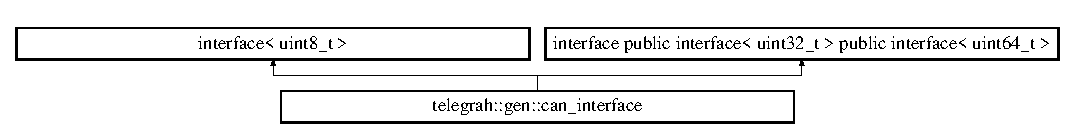
\includegraphics[height=1.421320cm]{classtelegrah_1_1gen_1_1can__interface}
\end{center}
\end{figure}
\subsection*{Public Member Functions}
\begin{DoxyCompactItemize}
\item 
void \hyperlink{classtelegrah_1_1gen_1_1can__interface_a86b5cb1f63f8287500a4245a7fb1d5cc}{send} (int16\+\_\+t id, uint8\+\_\+t len, uint8\+\_\+t $\ast$buf)=0
\end{DoxyCompactItemize}


\subsection{Member Function Documentation}
\mbox{\Hypertarget{classtelegrah_1_1gen_1_1can__interface_a86b5cb1f63f8287500a4245a7fb1d5cc}\label{classtelegrah_1_1gen_1_1can__interface_a86b5cb1f63f8287500a4245a7fb1d5cc}} 
\index{telegrah\+::gen\+::can\+\_\+interface@{telegrah\+::gen\+::can\+\_\+interface}!send@{send}}
\index{send@{send}!telegrah\+::gen\+::can\+\_\+interface@{telegrah\+::gen\+::can\+\_\+interface}}
\subsubsection{\texorpdfstring{send()}{send()}}
{\footnotesize\ttfamily void telegrah\+::gen\+::can\+\_\+interface\+::send (\begin{DoxyParamCaption}\item[{int16\+\_\+t}]{id,  }\item[{uint8\+\_\+t}]{len,  }\item[{uint8\+\_\+t $\ast$}]{buf }\end{DoxyParamCaption})\hspace{0.3cm}{\ttfamily [pure virtual]}}



The documentation for this class was generated from the following file\+:\begin{DoxyCompactItemize}
\item 
\hyperlink{can__interface_8hpp}{can\+\_\+interface.\+hpp}\end{DoxyCompactItemize}

\hypertarget{classtelegraph_1_1collection}{}\section{telegraph\+:\+:collection$<$ T $>$ Class Template Reference}
\label{classtelegraph_1_1collection}\index{telegraph\+::collection$<$ T $>$@{telegraph\+::collection$<$ T $>$}}


{\ttfamily \#include $<$collection.\+hpp$>$}

Inheritance diagram for telegraph\+:\+:collection$<$ T $>$\+:\begin{figure}[H]
\begin{center}
\leavevmode
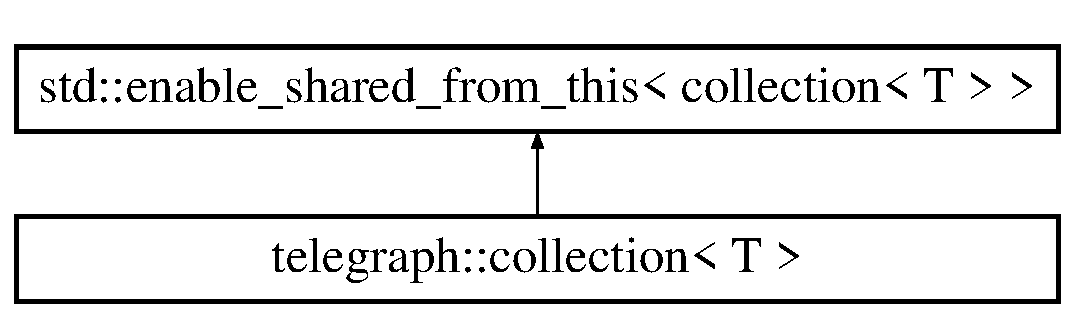
\includegraphics[height=2.000000cm]{classtelegraph_1_1collection}
\end{center}
\end{figure}
\subsection*{Public Types}
\begin{DoxyCompactItemize}
\item 
using \hyperlink{classtelegraph_1_1collection_a7d1c05b1bdcbe95a3127122969e14173}{key} = typename \hyperlink{structtelegraph_1_1collection__key}{collection\+\_\+key}$<$ T $>$\+::type
\end{DoxyCompactItemize}
\subsection*{Public Member Functions}
\begin{DoxyCompactItemize}
\item 
\hyperlink{classtelegraph_1_1collection_a226e589bb9d07937a82843f5da0610a0}{collection} ()
\item 
\hyperlink{classtelegraph_1_1collection_a4ce0e224a982a6025015a1ef7008ca56}{collection} (const std\+::shared\+\_\+ptr$<$ \hyperlink{classtelegraph_1_1collection}{collection} $>$ \&src, const std\+::function$<$ bool(const T \&)$>$ \&\hyperlink{classtelegraph_1_1collection_afa7564c9896fde9d965f422f8ee6a4ce}{filter})
\item 
std\+::shared\+\_\+ptr$<$ \hyperlink{classtelegraph_1_1collection}{collection} $>$ \hyperlink{classtelegraph_1_1collection_afa7564c9896fde9d965f422f8ee6a4ce}{filter} (const std\+::function$<$ bool(const T \&)$>$ \&f)
\item 
bool \hyperlink{classtelegraph_1_1collection_af9b482ee7d179bd7c4dfa47fba1df507}{has} (const \hyperlink{classtelegraph_1_1collection_a7d1c05b1bdcbe95a3127122969e14173}{key} \&k) const
\item 
constexpr size\+\_\+t \hyperlink{classtelegraph_1_1collection_ae51a6f64a8c24e2c602e6c3c4865249a}{size} () const
\item 
const T \& \hyperlink{classtelegraph_1_1collection_ac3c0fd37e9000e9de5ba9c3aeee330c1}{result} () const
\item 
T \hyperlink{classtelegraph_1_1collection_a3065b252176bd28f4280ad0384276e3e}{get} (const \hyperlink{classtelegraph_1_1collection_a7d1c05b1bdcbe95a3127122969e14173}{key} \&k) const
\item 
void \hyperlink{classtelegraph_1_1collection_af8383989a761fdd14631dd6c0e574298}{add\+\_\+} (const T \&v)
\item 
void \hyperlink{classtelegraph_1_1collection_ab736aff469340ac47c12c6b84ac9fd4d}{remove\+\_\+} (const T \&v)
\item 
void \hyperlink{classtelegraph_1_1collection_a0e9199b87fb87d2602fc6e4cc33835c7}{remove\+\_\+by\+\_\+key\+\_\+} (const \hyperlink{classtelegraph_1_1collection_a7d1c05b1bdcbe95a3127122969e14173}{key} \&k)
\item 
std\+::unordered\+\_\+map$<$ \hyperlink{classtelegraph_1_1collection_a7d1c05b1bdcbe95a3127122969e14173}{key}, T $>$\+::iterator \hyperlink{classtelegraph_1_1collection_a0bebe64fbda6ce9af9922531879099c3}{begin} ()
\item 
std\+::unordered\+\_\+map$<$ \hyperlink{classtelegraph_1_1collection_a7d1c05b1bdcbe95a3127122969e14173}{key}, T $>$\+::iterator \hyperlink{classtelegraph_1_1collection_a262da7d56b726b69ddee3de30f086066}{begin} () const
\item 
std\+::unordered\+\_\+map$<$ \hyperlink{classtelegraph_1_1collection_a7d1c05b1bdcbe95a3127122969e14173}{key}, T $>$\+::iterator \hyperlink{classtelegraph_1_1collection_a14b2edf6043f717d568342a1a7575132}{end} ()
\item 
std\+::unordered\+\_\+map$<$ \hyperlink{classtelegraph_1_1collection_a7d1c05b1bdcbe95a3127122969e14173}{key}, T $>$\+::iterator \hyperlink{classtelegraph_1_1collection_ae8833bbd79ee1d4bc8c4d4c949fc4532}{end} () const
\end{DoxyCompactItemize}
\subsection*{Public Attributes}
\begin{DoxyCompactItemize}
\item 
\hyperlink{classtelegraph_1_1signal}{signal}$<$ const T \& $>$ \hyperlink{classtelegraph_1_1collection_a7ac59f0f85680539f80d085dd35b3c47}{added}
\item 
\hyperlink{classtelegraph_1_1signal}{signal}$<$ const T \& $>$ \hyperlink{classtelegraph_1_1collection_a6fdb7502f6cef02065c6bbde435756f0}{removed}
\item 
std\+::unordered\+\_\+map$<$ \hyperlink{classtelegraph_1_1collection_a7d1c05b1bdcbe95a3127122969e14173}{key}, T $>$ \hyperlink{classtelegraph_1_1collection_a5a6329136af41edba2e17fddaaa5384c}{current}
\end{DoxyCompactItemize}


\subsection{Member Typedef Documentation}
\mbox{\Hypertarget{classtelegraph_1_1collection_a7d1c05b1bdcbe95a3127122969e14173}\label{classtelegraph_1_1collection_a7d1c05b1bdcbe95a3127122969e14173}} 
\index{telegraph\+::collection@{telegraph\+::collection}!key@{key}}
\index{key@{key}!telegraph\+::collection@{telegraph\+::collection}}
\subsubsection{\texorpdfstring{key}{key}}
{\footnotesize\ttfamily template$<$typename T $>$ \\
using \hyperlink{classtelegraph_1_1collection}{telegraph\+::collection}$<$ T $>$\+::\hyperlink{classtelegraph_1_1collection_a7d1c05b1bdcbe95a3127122969e14173}{key} =  typename \hyperlink{structtelegraph_1_1collection__key}{collection\+\_\+key}$<$T$>$\+::type}



\subsection{Constructor \& Destructor Documentation}
\mbox{\Hypertarget{classtelegraph_1_1collection_a226e589bb9d07937a82843f5da0610a0}\label{classtelegraph_1_1collection_a226e589bb9d07937a82843f5da0610a0}} 
\index{telegraph\+::collection@{telegraph\+::collection}!collection@{collection}}
\index{collection@{collection}!telegraph\+::collection@{telegraph\+::collection}}
\subsubsection{\texorpdfstring{collection()}{collection()}\hspace{0.1cm}{\footnotesize\ttfamily [1/2]}}
{\footnotesize\ttfamily template$<$typename T $>$ \\
\hyperlink{classtelegraph_1_1collection}{telegraph\+::collection}$<$ T $>$\+::\hyperlink{classtelegraph_1_1collection}{collection} (\begin{DoxyParamCaption}{ }\end{DoxyParamCaption})\hspace{0.3cm}{\ttfamily [inline]}}

\mbox{\Hypertarget{classtelegraph_1_1collection_a4ce0e224a982a6025015a1ef7008ca56}\label{classtelegraph_1_1collection_a4ce0e224a982a6025015a1ef7008ca56}} 
\index{telegraph\+::collection@{telegraph\+::collection}!collection@{collection}}
\index{collection@{collection}!telegraph\+::collection@{telegraph\+::collection}}
\subsubsection{\texorpdfstring{collection()}{collection()}\hspace{0.1cm}{\footnotesize\ttfamily [2/2]}}
{\footnotesize\ttfamily template$<$typename T $>$ \\
\hyperlink{classtelegraph_1_1collection}{telegraph\+::collection}$<$ T $>$\+::\hyperlink{classtelegraph_1_1collection}{collection} (\begin{DoxyParamCaption}\item[{const std\+::shared\+\_\+ptr$<$ \hyperlink{classtelegraph_1_1collection}{collection}$<$ T $>$ $>$ \&}]{src,  }\item[{const std\+::function$<$ bool(const T \&)$>$ \&}]{filter }\end{DoxyParamCaption})\hspace{0.3cm}{\ttfamily [inline]}}



\subsection{Member Function Documentation}
\mbox{\Hypertarget{classtelegraph_1_1collection_af8383989a761fdd14631dd6c0e574298}\label{classtelegraph_1_1collection_af8383989a761fdd14631dd6c0e574298}} 
\index{telegraph\+::collection@{telegraph\+::collection}!add\+\_\+@{add\+\_\+}}
\index{add\+\_\+@{add\+\_\+}!telegraph\+::collection@{telegraph\+::collection}}
\subsubsection{\texorpdfstring{add\+\_\+()}{add\_()}}
{\footnotesize\ttfamily template$<$typename T $>$ \\
void \hyperlink{classtelegraph_1_1collection}{telegraph\+::collection}$<$ T $>$\+::add\+\_\+ (\begin{DoxyParamCaption}\item[{const T \&}]{v }\end{DoxyParamCaption})\hspace{0.3cm}{\ttfamily [inline]}}

\mbox{\Hypertarget{classtelegraph_1_1collection_a0bebe64fbda6ce9af9922531879099c3}\label{classtelegraph_1_1collection_a0bebe64fbda6ce9af9922531879099c3}} 
\index{telegraph\+::collection@{telegraph\+::collection}!begin@{begin}}
\index{begin@{begin}!telegraph\+::collection@{telegraph\+::collection}}
\subsubsection{\texorpdfstring{begin()}{begin()}\hspace{0.1cm}{\footnotesize\ttfamily [1/2]}}
{\footnotesize\ttfamily template$<$typename T $>$ \\
std\+::unordered\+\_\+map$<$\hyperlink{classtelegraph_1_1collection_a7d1c05b1bdcbe95a3127122969e14173}{key}, T$>$\+::iterator \hyperlink{classtelegraph_1_1collection}{telegraph\+::collection}$<$ T $>$\+::begin (\begin{DoxyParamCaption}{ }\end{DoxyParamCaption})\hspace{0.3cm}{\ttfamily [inline]}}

\mbox{\Hypertarget{classtelegraph_1_1collection_a262da7d56b726b69ddee3de30f086066}\label{classtelegraph_1_1collection_a262da7d56b726b69ddee3de30f086066}} 
\index{telegraph\+::collection@{telegraph\+::collection}!begin@{begin}}
\index{begin@{begin}!telegraph\+::collection@{telegraph\+::collection}}
\subsubsection{\texorpdfstring{begin()}{begin()}\hspace{0.1cm}{\footnotesize\ttfamily [2/2]}}
{\footnotesize\ttfamily template$<$typename T $>$ \\
std\+::unordered\+\_\+map$<$\hyperlink{classtelegraph_1_1collection_a7d1c05b1bdcbe95a3127122969e14173}{key}, T$>$\+::iterator \hyperlink{classtelegraph_1_1collection}{telegraph\+::collection}$<$ T $>$\+::begin (\begin{DoxyParamCaption}{ }\end{DoxyParamCaption}) const\hspace{0.3cm}{\ttfamily [inline]}}

\mbox{\Hypertarget{classtelegraph_1_1collection_a14b2edf6043f717d568342a1a7575132}\label{classtelegraph_1_1collection_a14b2edf6043f717d568342a1a7575132}} 
\index{telegraph\+::collection@{telegraph\+::collection}!end@{end}}
\index{end@{end}!telegraph\+::collection@{telegraph\+::collection}}
\subsubsection{\texorpdfstring{end()}{end()}\hspace{0.1cm}{\footnotesize\ttfamily [1/2]}}
{\footnotesize\ttfamily template$<$typename T $>$ \\
std\+::unordered\+\_\+map$<$\hyperlink{classtelegraph_1_1collection_a7d1c05b1bdcbe95a3127122969e14173}{key}, T$>$\+::iterator \hyperlink{classtelegraph_1_1collection}{telegraph\+::collection}$<$ T $>$\+::end (\begin{DoxyParamCaption}{ }\end{DoxyParamCaption})\hspace{0.3cm}{\ttfamily [inline]}}

\mbox{\Hypertarget{classtelegraph_1_1collection_ae8833bbd79ee1d4bc8c4d4c949fc4532}\label{classtelegraph_1_1collection_ae8833bbd79ee1d4bc8c4d4c949fc4532}} 
\index{telegraph\+::collection@{telegraph\+::collection}!end@{end}}
\index{end@{end}!telegraph\+::collection@{telegraph\+::collection}}
\subsubsection{\texorpdfstring{end()}{end()}\hspace{0.1cm}{\footnotesize\ttfamily [2/2]}}
{\footnotesize\ttfamily template$<$typename T $>$ \\
std\+::unordered\+\_\+map$<$\hyperlink{classtelegraph_1_1collection_a7d1c05b1bdcbe95a3127122969e14173}{key}, T$>$\+::iterator \hyperlink{classtelegraph_1_1collection}{telegraph\+::collection}$<$ T $>$\+::end (\begin{DoxyParamCaption}{ }\end{DoxyParamCaption}) const\hspace{0.3cm}{\ttfamily [inline]}}

\mbox{\Hypertarget{classtelegraph_1_1collection_afa7564c9896fde9d965f422f8ee6a4ce}\label{classtelegraph_1_1collection_afa7564c9896fde9d965f422f8ee6a4ce}} 
\index{telegraph\+::collection@{telegraph\+::collection}!filter@{filter}}
\index{filter@{filter}!telegraph\+::collection@{telegraph\+::collection}}
\subsubsection{\texorpdfstring{filter()}{filter()}}
{\footnotesize\ttfamily template$<$typename T $>$ \\
std\+::shared\+\_\+ptr$<$\hyperlink{classtelegraph_1_1collection}{collection}$>$ \hyperlink{classtelegraph_1_1collection}{telegraph\+::collection}$<$ T $>$\+::filter (\begin{DoxyParamCaption}\item[{const std\+::function$<$ bool(const T \&)$>$ \&}]{f }\end{DoxyParamCaption})\hspace{0.3cm}{\ttfamily [inline]}}

\mbox{\Hypertarget{classtelegraph_1_1collection_a3065b252176bd28f4280ad0384276e3e}\label{classtelegraph_1_1collection_a3065b252176bd28f4280ad0384276e3e}} 
\index{telegraph\+::collection@{telegraph\+::collection}!get@{get}}
\index{get@{get}!telegraph\+::collection@{telegraph\+::collection}}
\subsubsection{\texorpdfstring{get()}{get()}}
{\footnotesize\ttfamily template$<$typename T $>$ \\
T \hyperlink{classtelegraph_1_1collection}{telegraph\+::collection}$<$ T $>$\+::get (\begin{DoxyParamCaption}\item[{const \hyperlink{classtelegraph_1_1collection_a7d1c05b1bdcbe95a3127122969e14173}{key} \&}]{k }\end{DoxyParamCaption}) const\hspace{0.3cm}{\ttfamily [inline]}}

\mbox{\Hypertarget{classtelegraph_1_1collection_af9b482ee7d179bd7c4dfa47fba1df507}\label{classtelegraph_1_1collection_af9b482ee7d179bd7c4dfa47fba1df507}} 
\index{telegraph\+::collection@{telegraph\+::collection}!has@{has}}
\index{has@{has}!telegraph\+::collection@{telegraph\+::collection}}
\subsubsection{\texorpdfstring{has()}{has()}}
{\footnotesize\ttfamily template$<$typename T $>$ \\
bool \hyperlink{classtelegraph_1_1collection}{telegraph\+::collection}$<$ T $>$\+::has (\begin{DoxyParamCaption}\item[{const \hyperlink{classtelegraph_1_1collection_a7d1c05b1bdcbe95a3127122969e14173}{key} \&}]{k }\end{DoxyParamCaption}) const\hspace{0.3cm}{\ttfamily [inline]}}

\mbox{\Hypertarget{classtelegraph_1_1collection_ab736aff469340ac47c12c6b84ac9fd4d}\label{classtelegraph_1_1collection_ab736aff469340ac47c12c6b84ac9fd4d}} 
\index{telegraph\+::collection@{telegraph\+::collection}!remove\+\_\+@{remove\+\_\+}}
\index{remove\+\_\+@{remove\+\_\+}!telegraph\+::collection@{telegraph\+::collection}}
\subsubsection{\texorpdfstring{remove\+\_\+()}{remove\_()}}
{\footnotesize\ttfamily template$<$typename T $>$ \\
void \hyperlink{classtelegraph_1_1collection}{telegraph\+::collection}$<$ T $>$\+::remove\+\_\+ (\begin{DoxyParamCaption}\item[{const T \&}]{v }\end{DoxyParamCaption})\hspace{0.3cm}{\ttfamily [inline]}}

\mbox{\Hypertarget{classtelegraph_1_1collection_a0e9199b87fb87d2602fc6e4cc33835c7}\label{classtelegraph_1_1collection_a0e9199b87fb87d2602fc6e4cc33835c7}} 
\index{telegraph\+::collection@{telegraph\+::collection}!remove\+\_\+by\+\_\+key\+\_\+@{remove\+\_\+by\+\_\+key\+\_\+}}
\index{remove\+\_\+by\+\_\+key\+\_\+@{remove\+\_\+by\+\_\+key\+\_\+}!telegraph\+::collection@{telegraph\+::collection}}
\subsubsection{\texorpdfstring{remove\+\_\+by\+\_\+key\+\_\+()}{remove\_by\_key\_()}}
{\footnotesize\ttfamily template$<$typename T $>$ \\
void \hyperlink{classtelegraph_1_1collection}{telegraph\+::collection}$<$ T $>$\+::remove\+\_\+by\+\_\+key\+\_\+ (\begin{DoxyParamCaption}\item[{const \hyperlink{classtelegraph_1_1collection_a7d1c05b1bdcbe95a3127122969e14173}{key} \&}]{k }\end{DoxyParamCaption})\hspace{0.3cm}{\ttfamily [inline]}}

\mbox{\Hypertarget{classtelegraph_1_1collection_ac3c0fd37e9000e9de5ba9c3aeee330c1}\label{classtelegraph_1_1collection_ac3c0fd37e9000e9de5ba9c3aeee330c1}} 
\index{telegraph\+::collection@{telegraph\+::collection}!result@{result}}
\index{result@{result}!telegraph\+::collection@{telegraph\+::collection}}
\subsubsection{\texorpdfstring{result()}{result()}}
{\footnotesize\ttfamily template$<$typename T $>$ \\
const T\& \hyperlink{classtelegraph_1_1collection}{telegraph\+::collection}$<$ T $>$\+::result (\begin{DoxyParamCaption}{ }\end{DoxyParamCaption}) const\hspace{0.3cm}{\ttfamily [inline]}}

\mbox{\Hypertarget{classtelegraph_1_1collection_ae51a6f64a8c24e2c602e6c3c4865249a}\label{classtelegraph_1_1collection_ae51a6f64a8c24e2c602e6c3c4865249a}} 
\index{telegraph\+::collection@{telegraph\+::collection}!size@{size}}
\index{size@{size}!telegraph\+::collection@{telegraph\+::collection}}
\subsubsection{\texorpdfstring{size()}{size()}}
{\footnotesize\ttfamily template$<$typename T $>$ \\
constexpr size\+\_\+t \hyperlink{classtelegraph_1_1collection}{telegraph\+::collection}$<$ T $>$\+::size (\begin{DoxyParamCaption}{ }\end{DoxyParamCaption}) const\hspace{0.3cm}{\ttfamily [inline]}}



\subsection{Member Data Documentation}
\mbox{\Hypertarget{classtelegraph_1_1collection_a7ac59f0f85680539f80d085dd35b3c47}\label{classtelegraph_1_1collection_a7ac59f0f85680539f80d085dd35b3c47}} 
\index{telegraph\+::collection@{telegraph\+::collection}!added@{added}}
\index{added@{added}!telegraph\+::collection@{telegraph\+::collection}}
\subsubsection{\texorpdfstring{added}{added}}
{\footnotesize\ttfamily template$<$typename T $>$ \\
\hyperlink{classtelegraph_1_1signal}{signal}$<$const T\&$>$ \hyperlink{classtelegraph_1_1collection}{telegraph\+::collection}$<$ T $>$\+::added}

\mbox{\Hypertarget{classtelegraph_1_1collection_a5a6329136af41edba2e17fddaaa5384c}\label{classtelegraph_1_1collection_a5a6329136af41edba2e17fddaaa5384c}} 
\index{telegraph\+::collection@{telegraph\+::collection}!current@{current}}
\index{current@{current}!telegraph\+::collection@{telegraph\+::collection}}
\subsubsection{\texorpdfstring{current}{current}}
{\footnotesize\ttfamily template$<$typename T $>$ \\
std\+::unordered\+\_\+map$<$\hyperlink{classtelegraph_1_1collection_a7d1c05b1bdcbe95a3127122969e14173}{key}, T$>$ \hyperlink{classtelegraph_1_1collection}{telegraph\+::collection}$<$ T $>$\+::current}

\mbox{\Hypertarget{classtelegraph_1_1collection_a6fdb7502f6cef02065c6bbde435756f0}\label{classtelegraph_1_1collection_a6fdb7502f6cef02065c6bbde435756f0}} 
\index{telegraph\+::collection@{telegraph\+::collection}!removed@{removed}}
\index{removed@{removed}!telegraph\+::collection@{telegraph\+::collection}}
\subsubsection{\texorpdfstring{removed}{removed}}
{\footnotesize\ttfamily template$<$typename T $>$ \\
\hyperlink{classtelegraph_1_1signal}{signal}$<$const T\&$>$ \hyperlink{classtelegraph_1_1collection}{telegraph\+::collection}$<$ T $>$\+::removed}



The documentation for this class was generated from the following file\+:\begin{DoxyCompactItemize}
\item 
\hyperlink{collection_8hpp}{collection.\+hpp}\end{DoxyCompactItemize}

\hypertarget{structtelegraph_1_1collection__key}{}\section{telegraph\+:\+:collection\+\_\+key$<$ T $>$ Struct Template Reference}
\label{structtelegraph_1_1collection__key}\index{telegraph\+::collection\+\_\+key$<$ T $>$@{telegraph\+::collection\+\_\+key$<$ T $>$}}


{\ttfamily \#include $<$collection.\+hpp$>$}

\subsection*{Public Types}
\begin{DoxyCompactItemize}
\item 
typedef T \hyperlink{structtelegraph_1_1collection__key_a8f170ae277cbff0e224232c6f909a945}{type}
\end{DoxyCompactItemize}
\subsection*{Static Public Member Functions}
\begin{DoxyCompactItemize}
\item 
static \hyperlink{structtelegraph_1_1collection__key_a8f170ae277cbff0e224232c6f909a945}{type} \hyperlink{structtelegraph_1_1collection__key_a997f4a2971254f1ba4eebb900ce9d25c}{get} (const T \&v)
\end{DoxyCompactItemize}


\subsection{Member Typedef Documentation}
\mbox{\Hypertarget{structtelegraph_1_1collection__key_a8f170ae277cbff0e224232c6f909a945}\label{structtelegraph_1_1collection__key_a8f170ae277cbff0e224232c6f909a945}} 
\index{telegraph\+::collection\+\_\+key@{telegraph\+::collection\+\_\+key}!type@{type}}
\index{type@{type}!telegraph\+::collection\+\_\+key@{telegraph\+::collection\+\_\+key}}
\subsubsection{\texorpdfstring{type}{type}}
{\footnotesize\ttfamily template$<$typename T$>$ \\
typedef T \hyperlink{structtelegraph_1_1collection__key}{telegraph\+::collection\+\_\+key}$<$ T $>$\+::\hyperlink{structtelegraph_1_1collection__key_a8f170ae277cbff0e224232c6f909a945}{type}}



\subsection{Member Function Documentation}
\mbox{\Hypertarget{structtelegraph_1_1collection__key_a997f4a2971254f1ba4eebb900ce9d25c}\label{structtelegraph_1_1collection__key_a997f4a2971254f1ba4eebb900ce9d25c}} 
\index{telegraph\+::collection\+\_\+key@{telegraph\+::collection\+\_\+key}!get@{get}}
\index{get@{get}!telegraph\+::collection\+\_\+key@{telegraph\+::collection\+\_\+key}}
\subsubsection{\texorpdfstring{get()}{get()}}
{\footnotesize\ttfamily template$<$typename T$>$ \\
static \hyperlink{structtelegraph_1_1collection__key_a8f170ae277cbff0e224232c6f909a945}{type} \hyperlink{structtelegraph_1_1collection__key}{telegraph\+::collection\+\_\+key}$<$ T $>$\+::get (\begin{DoxyParamCaption}\item[{const T \&}]{v }\end{DoxyParamCaption})\hspace{0.3cm}{\ttfamily [inline]}, {\ttfamily [static]}}



The documentation for this struct was generated from the following file\+:\begin{DoxyCompactItemize}
\item 
\hyperlink{collection_8hpp}{collection.\+hpp}\end{DoxyCompactItemize}

\hypertarget{structtelegraph_1_1collection__key_3_01std_1_1shared__ptr_3_01context_01_4_01_4}{}\section{telegraph\+:\+:collection\+\_\+key$<$ std\+:\+:shared\+\_\+ptr$<$ context $>$ $>$ Struct Template Reference}
\label{structtelegraph_1_1collection__key_3_01std_1_1shared__ptr_3_01context_01_4_01_4}\index{telegraph\+::collection\+\_\+key$<$ std\+::shared\+\_\+ptr$<$ context $>$ $>$@{telegraph\+::collection\+\_\+key$<$ std\+::shared\+\_\+ptr$<$ context $>$ $>$}}


{\ttfamily \#include $<$namespace.\+hpp$>$}

\subsection*{Public Types}
\begin{DoxyCompactItemize}
\item 
typedef \hyperlink{namespacetelegraph_a51ee91d7eaeef067f7ccac2b170e5d59}{uuid} \hyperlink{structtelegraph_1_1collection__key_3_01std_1_1shared__ptr_3_01context_01_4_01_4_af7ea62096d0cff1cce249a8b4ad37f8b}{type}
\end{DoxyCompactItemize}
\subsection*{Static Public Member Functions}
\begin{DoxyCompactItemize}
\item 
static \hyperlink{namespacetelegraph_a51ee91d7eaeef067f7ccac2b170e5d59}{uuid} \hyperlink{structtelegraph_1_1collection__key_3_01std_1_1shared__ptr_3_01context_01_4_01_4_a35cb92d2d9c4516b4a0b9891f177cf05}{get} (const std\+::shared\+\_\+ptr$<$ \hyperlink{classtelegraph_1_1context}{context} $>$ \&c)
\end{DoxyCompactItemize}


\subsection{Member Typedef Documentation}
\mbox{\Hypertarget{structtelegraph_1_1collection__key_3_01std_1_1shared__ptr_3_01context_01_4_01_4_af7ea62096d0cff1cce249a8b4ad37f8b}\label{structtelegraph_1_1collection__key_3_01std_1_1shared__ptr_3_01context_01_4_01_4_af7ea62096d0cff1cce249a8b4ad37f8b}} 
\index{telegraph\+::collection\+\_\+key$<$ std\+::shared\+\_\+ptr$<$ context $>$ $>$@{telegraph\+::collection\+\_\+key$<$ std\+::shared\+\_\+ptr$<$ context $>$ $>$}!type@{type}}
\index{type@{type}!telegraph\+::collection\+\_\+key$<$ std\+::shared\+\_\+ptr$<$ context $>$ $>$@{telegraph\+::collection\+\_\+key$<$ std\+::shared\+\_\+ptr$<$ context $>$ $>$}}
\subsubsection{\texorpdfstring{type}{type}}
{\footnotesize\ttfamily typedef \hyperlink{namespacetelegraph_a51ee91d7eaeef067f7ccac2b170e5d59}{uuid} \hyperlink{structtelegraph_1_1collection__key}{telegraph\+::collection\+\_\+key}$<$ std\+::shared\+\_\+ptr$<$ \hyperlink{classtelegraph_1_1context}{context} $>$ $>$\+::\hyperlink{structtelegraph_1_1collection__key_3_01std_1_1shared__ptr_3_01context_01_4_01_4_af7ea62096d0cff1cce249a8b4ad37f8b}{type}}



\subsection{Member Function Documentation}
\mbox{\Hypertarget{structtelegraph_1_1collection__key_3_01std_1_1shared__ptr_3_01context_01_4_01_4_a35cb92d2d9c4516b4a0b9891f177cf05}\label{structtelegraph_1_1collection__key_3_01std_1_1shared__ptr_3_01context_01_4_01_4_a35cb92d2d9c4516b4a0b9891f177cf05}} 
\index{telegraph\+::collection\+\_\+key$<$ std\+::shared\+\_\+ptr$<$ context $>$ $>$@{telegraph\+::collection\+\_\+key$<$ std\+::shared\+\_\+ptr$<$ context $>$ $>$}!get@{get}}
\index{get@{get}!telegraph\+::collection\+\_\+key$<$ std\+::shared\+\_\+ptr$<$ context $>$ $>$@{telegraph\+::collection\+\_\+key$<$ std\+::shared\+\_\+ptr$<$ context $>$ $>$}}
\subsubsection{\texorpdfstring{get()}{get()}}
{\footnotesize\ttfamily static \hyperlink{namespacetelegraph_a51ee91d7eaeef067f7ccac2b170e5d59}{uuid} \hyperlink{structtelegraph_1_1collection__key}{telegraph\+::collection\+\_\+key}$<$ std\+::shared\+\_\+ptr$<$ \hyperlink{classtelegraph_1_1context}{context} $>$ $>$\+::get (\begin{DoxyParamCaption}\item[{const std\+::shared\+\_\+ptr$<$ \hyperlink{classtelegraph_1_1context}{context} $>$ \&}]{c }\end{DoxyParamCaption})\hspace{0.3cm}{\ttfamily [inline]}, {\ttfamily [static]}}



The documentation for this struct was generated from the following file\+:\begin{DoxyCompactItemize}
\item 
\hyperlink{common_2namespace_8hpp}{common/namespace.\+hpp}\end{DoxyCompactItemize}

\hypertarget{classtelegraph_1_1config}{}\section{telegraph\+:\+:config Class Reference}
\label{classtelegraph_1_1config}\index{telegraph\+::config@{telegraph\+::config}}


{\ttfamily \#include $<$config.\+hpp$>$}

\subsection*{Public Member Functions}
\begin{DoxyCompactItemize}
\item 
\hyperlink{classtelegraph_1_1config_a5f3f45e1e31d82f52c0242f7cb14083c}{config} (const \hyperlink{namespacetelegraph_ab87b47a6b955c365ddd74c343ecc16f4}{json} \&j)
\item 
\hyperlink{classtelegraph_1_1config_a58461425cd48e9ce43eeaf5cffdf68ba}{$\sim$config} ()
\item 
const \hyperlink{classtelegraph_1_1node}{node} $\ast$ \hyperlink{classtelegraph_1_1config_a037e49fa107a7d738747caa7212388ad}{get\+\_\+tree} () const
\item 
\hyperlink{classtelegraph_1_1profile}{profile} \& \hyperlink{classtelegraph_1_1config_a9002a994691d15a3252c3fd23eaca014}{get\+\_\+profile} (const std\+::string \&name)
\item 
const \hyperlink{classtelegraph_1_1profile}{profile} \& \hyperlink{classtelegraph_1_1config_a7a8ab41521fa4af8d17d009c3872fb87}{get\+\_\+profile} (const std\+::string \&name) const
\end{DoxyCompactItemize}


\subsection{Constructor \& Destructor Documentation}
\mbox{\Hypertarget{classtelegraph_1_1config_a5f3f45e1e31d82f52c0242f7cb14083c}\label{classtelegraph_1_1config_a5f3f45e1e31d82f52c0242f7cb14083c}} 
\index{telegraph\+::config@{telegraph\+::config}!config@{config}}
\index{config@{config}!telegraph\+::config@{telegraph\+::config}}
\subsubsection{\texorpdfstring{config()}{config()}}
{\footnotesize\ttfamily telegraph\+::config\+::config (\begin{DoxyParamCaption}\item[{const \hyperlink{namespacetelegraph_ab87b47a6b955c365ddd74c343ecc16f4}{json} \&}]{j }\end{DoxyParamCaption})}

\mbox{\Hypertarget{classtelegraph_1_1config_a58461425cd48e9ce43eeaf5cffdf68ba}\label{classtelegraph_1_1config_a58461425cd48e9ce43eeaf5cffdf68ba}} 
\index{telegraph\+::config@{telegraph\+::config}!````~config@{$\sim$config}}
\index{````~config@{$\sim$config}!telegraph\+::config@{telegraph\+::config}}
\subsubsection{\texorpdfstring{$\sim$config()}{~config()}}
{\footnotesize\ttfamily telegraph\+::config\+::$\sim$config (\begin{DoxyParamCaption}{ }\end{DoxyParamCaption})}



\subsection{Member Function Documentation}
\mbox{\Hypertarget{classtelegraph_1_1config_a9002a994691d15a3252c3fd23eaca014}\label{classtelegraph_1_1config_a9002a994691d15a3252c3fd23eaca014}} 
\index{telegraph\+::config@{telegraph\+::config}!get\+\_\+profile@{get\+\_\+profile}}
\index{get\+\_\+profile@{get\+\_\+profile}!telegraph\+::config@{telegraph\+::config}}
\subsubsection{\texorpdfstring{get\+\_\+profile()}{get\_profile()}\hspace{0.1cm}{\footnotesize\ttfamily [1/2]}}
{\footnotesize\ttfamily \hyperlink{classtelegraph_1_1profile}{profile}\& telegraph\+::config\+::get\+\_\+profile (\begin{DoxyParamCaption}\item[{const std\+::string \&}]{name }\end{DoxyParamCaption})\hspace{0.3cm}{\ttfamily [inline]}}

\mbox{\Hypertarget{classtelegraph_1_1config_a7a8ab41521fa4af8d17d009c3872fb87}\label{classtelegraph_1_1config_a7a8ab41521fa4af8d17d009c3872fb87}} 
\index{telegraph\+::config@{telegraph\+::config}!get\+\_\+profile@{get\+\_\+profile}}
\index{get\+\_\+profile@{get\+\_\+profile}!telegraph\+::config@{telegraph\+::config}}
\subsubsection{\texorpdfstring{get\+\_\+profile()}{get\_profile()}\hspace{0.1cm}{\footnotesize\ttfamily [2/2]}}
{\footnotesize\ttfamily const \hyperlink{classtelegraph_1_1profile}{profile}\& telegraph\+::config\+::get\+\_\+profile (\begin{DoxyParamCaption}\item[{const std\+::string \&}]{name }\end{DoxyParamCaption}) const\hspace{0.3cm}{\ttfamily [inline]}}

\mbox{\Hypertarget{classtelegraph_1_1config_a037e49fa107a7d738747caa7212388ad}\label{classtelegraph_1_1config_a037e49fa107a7d738747caa7212388ad}} 
\index{telegraph\+::config@{telegraph\+::config}!get\+\_\+tree@{get\+\_\+tree}}
\index{get\+\_\+tree@{get\+\_\+tree}!telegraph\+::config@{telegraph\+::config}}
\subsubsection{\texorpdfstring{get\+\_\+tree()}{get\_tree()}}
{\footnotesize\ttfamily const \hyperlink{classtelegraph_1_1node}{node}$\ast$ telegraph\+::config\+::get\+\_\+tree (\begin{DoxyParamCaption}{ }\end{DoxyParamCaption}) const\hspace{0.3cm}{\ttfamily [inline]}}



The documentation for this class was generated from the following files\+:\begin{DoxyCompactItemize}
\item 
\hyperlink{config_8hpp}{config.\+hpp}\item 
\hyperlink{config_8cpp}{config.\+cpp}\end{DoxyCompactItemize}

\hypertarget{classtelegraph_1_1connection}{}\section{telegraph\+:\+:connection Class Reference}
\label{classtelegraph_1_1connection}\index{telegraph\+::connection@{telegraph\+::connection}}


{\ttfamily \#include $<$connection.\+hpp$>$}

Inheritance diagram for telegraph\+:\+:connection\+:\begin{figure}[H]
\begin{center}
\leavevmode
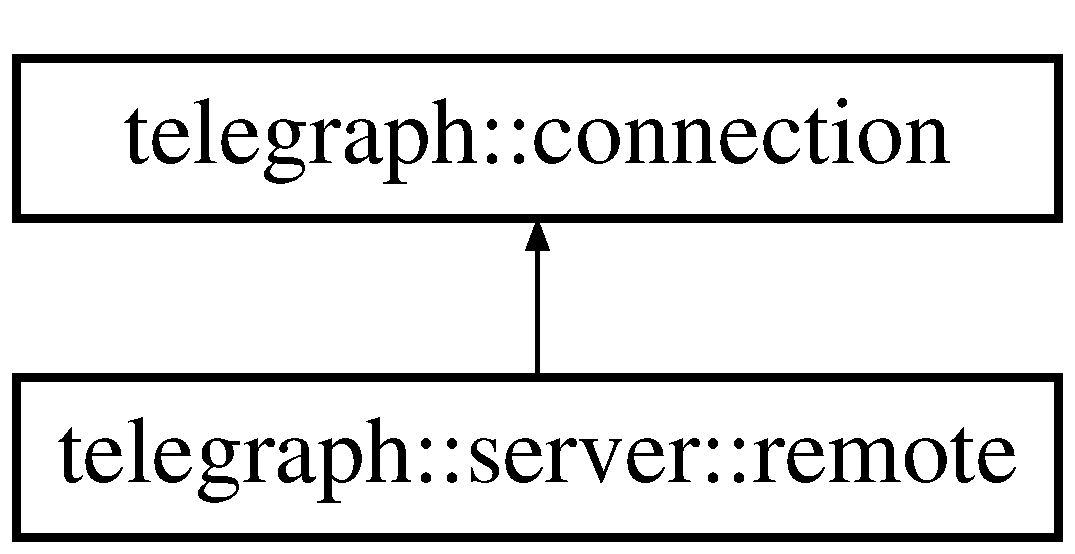
\includegraphics[height=2.000000cm]{classtelegraph_1_1connection}
\end{center}
\end{figure}
\subsection*{Public Member Functions}
\begin{DoxyCompactItemize}
\item 
\hyperlink{classtelegraph_1_1connection_a6952fb62edd1c7e78fe8744d4eac7aaa}{connection} (io\+::io\+\_\+context \&ioc, bool count\+\_\+down)
\item 
\hyperlink{classtelegraph_1_1connection_a469b53662900132cfc89a595b1dab28c}{$\sim$connection} ()
\item 
void \hyperlink{classtelegraph_1_1connection_a6dd7c859165db61ecdd14a8e5bcc7fcf}{received} (\hyperlink{structboost_1_1asio_1_1yield__ctx}{io\+::yield\+\_\+ctx} \&yield, const api\+::\+Packet \&p)
\item 
virtual void \hyperlink{classtelegraph_1_1connection_ad5fd2c23680ecda6e07c2f02f3735809}{send} (api\+::\+Packet \&\&p)=0
\item 
api\+::\+Packet \hyperlink{classtelegraph_1_1connection_a5edeb1d722fad636d63f125d896e41c4}{request\+\_\+response} (\hyperlink{structboost_1_1asio_1_1yield__ctx}{io\+::yield\+\_\+ctx} \&yield, api\+::\+Packet \&\&req)
\item 
api\+::\+Packet \hyperlink{classtelegraph_1_1connection_a769414199f9cf151ff115f223f07fb5c}{request\+\_\+stream} (\hyperlink{structboost_1_1asio_1_1yield__ctx}{io\+::yield\+\_\+ctx} \&yield, api\+::\+Packet \&\&req, const handler \&cb)
\item 
void \hyperlink{classtelegraph_1_1connection_a07cd6d890aad0f708ca32d136e063937}{set\+\_\+handler} (api\+::\+Packet\+::\+Payload\+Case c, const handler \&h)
\item 
void \hyperlink{classtelegraph_1_1connection_ad3ec8072dd935d37eaac8cbc2390177d}{set\+\_\+stream\+\_\+cb} (int32\+\_\+t req\+\_\+id, const handler \&h)
\item 
void \hyperlink{classtelegraph_1_1connection_a5bf70bff51c2cd812f4f27b3e37e9060}{write\+\_\+back} (int32\+\_\+t req\+\_\+id, api\+::\+Packet \&\&p)
\item 
void \hyperlink{classtelegraph_1_1connection_a8c977ff1083d9457444cee0cc4fc1add}{close\+\_\+stream} (int32\+\_\+t req\+\_\+id)
\end{DoxyCompactItemize}


\subsection{Constructor \& Destructor Documentation}
\mbox{\Hypertarget{classtelegraph_1_1connection_a6952fb62edd1c7e78fe8744d4eac7aaa}\label{classtelegraph_1_1connection_a6952fb62edd1c7e78fe8744d4eac7aaa}} 
\index{telegraph\+::connection@{telegraph\+::connection}!connection@{connection}}
\index{connection@{connection}!telegraph\+::connection@{telegraph\+::connection}}
\subsubsection{\texorpdfstring{connection()}{connection()}}
{\footnotesize\ttfamily telegraph\+::connection\+::connection (\begin{DoxyParamCaption}\item[{io\+::io\+\_\+context \&}]{ioc,  }\item[{bool}]{count\+\_\+down }\end{DoxyParamCaption})}

\mbox{\Hypertarget{classtelegraph_1_1connection_a469b53662900132cfc89a595b1dab28c}\label{classtelegraph_1_1connection_a469b53662900132cfc89a595b1dab28c}} 
\index{telegraph\+::connection@{telegraph\+::connection}!````~connection@{$\sim$connection}}
\index{````~connection@{$\sim$connection}!telegraph\+::connection@{telegraph\+::connection}}
\subsubsection{\texorpdfstring{$\sim$connection()}{~connection()}}
{\footnotesize\ttfamily telegraph\+::connection\+::$\sim$connection (\begin{DoxyParamCaption}{ }\end{DoxyParamCaption})}



\subsection{Member Function Documentation}
\mbox{\Hypertarget{classtelegraph_1_1connection_a8c977ff1083d9457444cee0cc4fc1add}\label{classtelegraph_1_1connection_a8c977ff1083d9457444cee0cc4fc1add}} 
\index{telegraph\+::connection@{telegraph\+::connection}!close\+\_\+stream@{close\+\_\+stream}}
\index{close\+\_\+stream@{close\+\_\+stream}!telegraph\+::connection@{telegraph\+::connection}}
\subsubsection{\texorpdfstring{close\+\_\+stream()}{close\_stream()}}
{\footnotesize\ttfamily void telegraph\+::connection\+::close\+\_\+stream (\begin{DoxyParamCaption}\item[{int32\+\_\+t}]{req\+\_\+id }\end{DoxyParamCaption})}

\mbox{\Hypertarget{classtelegraph_1_1connection_a6dd7c859165db61ecdd14a8e5bcc7fcf}\label{classtelegraph_1_1connection_a6dd7c859165db61ecdd14a8e5bcc7fcf}} 
\index{telegraph\+::connection@{telegraph\+::connection}!received@{received}}
\index{received@{received}!telegraph\+::connection@{telegraph\+::connection}}
\subsubsection{\texorpdfstring{received()}{received()}}
{\footnotesize\ttfamily void telegraph\+::connection\+::received (\begin{DoxyParamCaption}\item[{\hyperlink{structboost_1_1asio_1_1yield__ctx}{io\+::yield\+\_\+ctx} \&}]{yield,  }\item[{const api\+::\+Packet \&}]{p }\end{DoxyParamCaption})}

\mbox{\Hypertarget{classtelegraph_1_1connection_a5edeb1d722fad636d63f125d896e41c4}\label{classtelegraph_1_1connection_a5edeb1d722fad636d63f125d896e41c4}} 
\index{telegraph\+::connection@{telegraph\+::connection}!request\+\_\+response@{request\+\_\+response}}
\index{request\+\_\+response@{request\+\_\+response}!telegraph\+::connection@{telegraph\+::connection}}
\subsubsection{\texorpdfstring{request\+\_\+response()}{request\_response()}}
{\footnotesize\ttfamily api\+::\+Packet telegraph\+::connection\+::request\+\_\+response (\begin{DoxyParamCaption}\item[{\hyperlink{structboost_1_1asio_1_1yield__ctx}{io\+::yield\+\_\+ctx} \&}]{yield,  }\item[{api\+::\+Packet \&\&}]{req }\end{DoxyParamCaption})}

\mbox{\Hypertarget{classtelegraph_1_1connection_a769414199f9cf151ff115f223f07fb5c}\label{classtelegraph_1_1connection_a769414199f9cf151ff115f223f07fb5c}} 
\index{telegraph\+::connection@{telegraph\+::connection}!request\+\_\+stream@{request\+\_\+stream}}
\index{request\+\_\+stream@{request\+\_\+stream}!telegraph\+::connection@{telegraph\+::connection}}
\subsubsection{\texorpdfstring{request\+\_\+stream()}{request\_stream()}}
{\footnotesize\ttfamily api\+::\+Packet telegraph\+::connection\+::request\+\_\+stream (\begin{DoxyParamCaption}\item[{\hyperlink{structboost_1_1asio_1_1yield__ctx}{io\+::yield\+\_\+ctx} \&}]{yield,  }\item[{api\+::\+Packet \&\&}]{req,  }\item[{const handler \&}]{cb }\end{DoxyParamCaption})}

\mbox{\Hypertarget{classtelegraph_1_1connection_ad5fd2c23680ecda6e07c2f02f3735809}\label{classtelegraph_1_1connection_ad5fd2c23680ecda6e07c2f02f3735809}} 
\index{telegraph\+::connection@{telegraph\+::connection}!send@{send}}
\index{send@{send}!telegraph\+::connection@{telegraph\+::connection}}
\subsubsection{\texorpdfstring{send()}{send()}}
{\footnotesize\ttfamily virtual void telegraph\+::connection\+::send (\begin{DoxyParamCaption}\item[{api\+::\+Packet \&\&}]{p }\end{DoxyParamCaption})\hspace{0.3cm}{\ttfamily [pure virtual]}}



Implemented in \hyperlink{classtelegraph_1_1server_1_1remote_aa6a2f2d4045ea8bb51938ca3da4e1b5e}{telegraph\+::server\+::remote}.

\mbox{\Hypertarget{classtelegraph_1_1connection_a07cd6d890aad0f708ca32d136e063937}\label{classtelegraph_1_1connection_a07cd6d890aad0f708ca32d136e063937}} 
\index{telegraph\+::connection@{telegraph\+::connection}!set\+\_\+handler@{set\+\_\+handler}}
\index{set\+\_\+handler@{set\+\_\+handler}!telegraph\+::connection@{telegraph\+::connection}}
\subsubsection{\texorpdfstring{set\+\_\+handler()}{set\_handler()}}
{\footnotesize\ttfamily void telegraph\+::connection\+::set\+\_\+handler (\begin{DoxyParamCaption}\item[{api\+::\+Packet\+::\+Payload\+Case}]{c,  }\item[{const handler \&}]{h }\end{DoxyParamCaption})}

\mbox{\Hypertarget{classtelegraph_1_1connection_ad3ec8072dd935d37eaac8cbc2390177d}\label{classtelegraph_1_1connection_ad3ec8072dd935d37eaac8cbc2390177d}} 
\index{telegraph\+::connection@{telegraph\+::connection}!set\+\_\+stream\+\_\+cb@{set\+\_\+stream\+\_\+cb}}
\index{set\+\_\+stream\+\_\+cb@{set\+\_\+stream\+\_\+cb}!telegraph\+::connection@{telegraph\+::connection}}
\subsubsection{\texorpdfstring{set\+\_\+stream\+\_\+cb()}{set\_stream\_cb()}}
{\footnotesize\ttfamily void telegraph\+::connection\+::set\+\_\+stream\+\_\+cb (\begin{DoxyParamCaption}\item[{int32\+\_\+t}]{req\+\_\+id,  }\item[{const handler \&}]{h }\end{DoxyParamCaption})}

\mbox{\Hypertarget{classtelegraph_1_1connection_a5bf70bff51c2cd812f4f27b3e37e9060}\label{classtelegraph_1_1connection_a5bf70bff51c2cd812f4f27b3e37e9060}} 
\index{telegraph\+::connection@{telegraph\+::connection}!write\+\_\+back@{write\+\_\+back}}
\index{write\+\_\+back@{write\+\_\+back}!telegraph\+::connection@{telegraph\+::connection}}
\subsubsection{\texorpdfstring{write\+\_\+back()}{write\_back()}}
{\footnotesize\ttfamily void telegraph\+::connection\+::write\+\_\+back (\begin{DoxyParamCaption}\item[{int32\+\_\+t}]{req\+\_\+id,  }\item[{api\+::\+Packet \&\&}]{p }\end{DoxyParamCaption})}



The documentation for this class was generated from the following files\+:\begin{DoxyCompactItemize}
\item 
\hyperlink{connection_8hpp}{connection.\+hpp}\item 
\hyperlink{connection_8cpp}{connection.\+cpp}\end{DoxyCompactItemize}

\hypertarget{classtelegraph_1_1container}{}\section{telegraph\+:\+:container Class Reference}
\label{classtelegraph_1_1container}\index{telegraph\+::container@{telegraph\+::container}}


{\ttfamily \#include $<$container.\+hpp$>$}

Inheritance diagram for telegraph\+:\+:container\+:\begin{figure}[H]
\begin{center}
\leavevmode
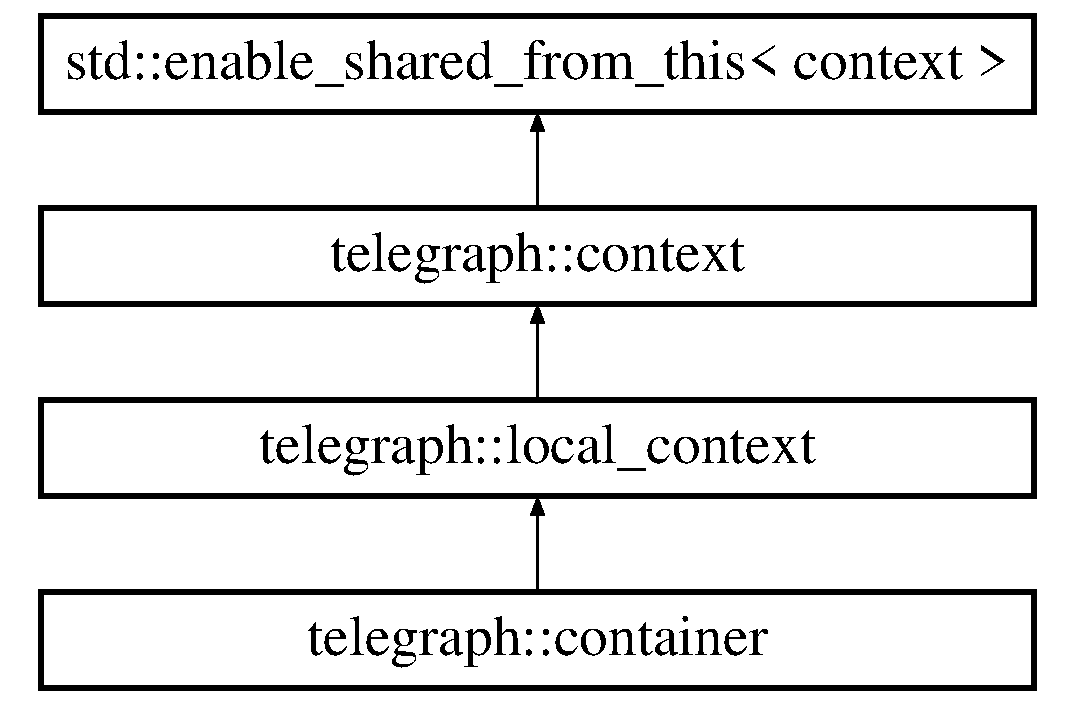
\includegraphics[height=4.000000cm]{classtelegraph_1_1container}
\end{center}
\end{figure}
\subsection*{Public Member Functions}
\begin{DoxyCompactItemize}
\item 
\hyperlink{classtelegraph_1_1container_a1bdc819f7250ab657c2b512994b2a4d9}{container} (io\+::io\+\_\+context \&ioc, const std\+::string\+\_\+view \&name, std\+::unique\+\_\+ptr$<$ \hyperlink{classtelegraph_1_1node}{node} $>$ \&\&tree, std\+::vector$<$ \hyperlink{namespacetelegraph_a332e681f0d44a1308cf3a013a9dd140f}{context\+\_\+ptr} $>$ \&\&mounts)
\item 
\hyperlink{classtelegraph_1_1container_a8f6afe0f414694ed550d654e722e4ae4}{$\sim$container} ()
\item 
\hyperlink{namespacetelegraph_ad071241508ea0f86c7de0686016f9ca9}{params\+\_\+stream\+\_\+ptr} \hyperlink{classtelegraph_1_1container_ade9ce299ee72554a84c1a71f0ad37915}{request} (\hyperlink{structboost_1_1asio_1_1yield__ctx}{io\+::yield\+\_\+ctx} \&, const \hyperlink{classtelegraph_1_1params}{params} \&p) override
\item 
\hyperlink{namespacetelegraph_a58641aa5b1a2cbdb0431916a87069f64}{subscription\+\_\+ptr} \hyperlink{classtelegraph_1_1container_ae1ae26a08bf3d367bbc13020623780b2}{subscribe} (\hyperlink{structboost_1_1asio_1_1yield__ctx}{io\+::yield\+\_\+ctx} \&ctx, const std\+::vector$<$ std\+::string\+\_\+view $>$ \&\hyperlink{classtelegraph_1_1variable}{variable}, float min\+\_\+interval, float max\+\_\+interval, float timeout) override
\item 
\hyperlink{namespacetelegraph_a58641aa5b1a2cbdb0431916a87069f64}{subscription\+\_\+ptr} \hyperlink{classtelegraph_1_1container_aa11f4e622d784b566a032c05f2019264}{subscribe} (\hyperlink{structboost_1_1asio_1_1yield__ctx}{io\+::yield\+\_\+ctx} \&ctx, const \hyperlink{classtelegraph_1_1variable}{variable} $\ast$v, float min\+\_\+interval, float max\+\_\+interval, float timeout) override
\item 
\hyperlink{classtelegraph_1_1value}{value} \hyperlink{classtelegraph_1_1container_a499649499d61f07dbe44bbec933414a0}{call} (\hyperlink{structboost_1_1asio_1_1yield__ctx}{io\+::yield\+\_\+ctx} \&yield, \hyperlink{classtelegraph_1_1action}{action} $\ast$a, \hyperlink{classtelegraph_1_1value}{value} v, float timeout) override
\item 
\hyperlink{classtelegraph_1_1value}{value} \hyperlink{classtelegraph_1_1container_a83d26f574b7f75655be9752147e30dce}{call} (\hyperlink{structboost_1_1asio_1_1yield__ctx}{io\+::yield\+\_\+ctx} \&yield, const std\+::vector$<$ std\+::string\+\_\+view $>$ \&a, \hyperlink{classtelegraph_1_1value}{value} v, float timeout) override
\item 
bool \hyperlink{classtelegraph_1_1container_aad8390913b2961a2270e6d4065deb59b}{write\+\_\+data} (\hyperlink{structboost_1_1asio_1_1yield__ctx}{io\+::yield\+\_\+ctx} \&yield, \hyperlink{classtelegraph_1_1variable}{variable} $\ast$v, const std\+::vector$<$ \hyperlink{classtelegraph_1_1data__point}{data\+\_\+point} $>$ \&data) override
\item 
bool \hyperlink{classtelegraph_1_1container_a6c608535adf0fee7783f6684ab4b69c8}{write\+\_\+data} (\hyperlink{structboost_1_1asio_1_1yield__ctx}{io\+::yield\+\_\+ctx} \&yield, const std\+::vector$<$ std\+::string\+\_\+view $>$ \&, const std\+::vector$<$ \hyperlink{classtelegraph_1_1data__point}{data\+\_\+point} $>$ \&data) override
\item 
\hyperlink{namespacetelegraph_a6ffe775ac48dca2a4013b53d692199c8}{data\+\_\+query\+\_\+ptr} \hyperlink{classtelegraph_1_1container_a1a9849e53091061da81e7c1a73502e47}{query\+\_\+data} (\hyperlink{structboost_1_1asio_1_1yield__ctx}{io\+::yield\+\_\+ctx} \&yield, const \hyperlink{classtelegraph_1_1variable}{variable} $\ast$v) override
\item 
\hyperlink{namespacetelegraph_a6ffe775ac48dca2a4013b53d692199c8}{data\+\_\+query\+\_\+ptr} \hyperlink{classtelegraph_1_1container_aca8b0b22be3cde48f0bc5f3fa79b29da}{query\+\_\+data} (\hyperlink{structboost_1_1asio_1_1yield__ctx}{io\+::yield\+\_\+ctx} \&yield, const std\+::vector$<$ std\+::string\+\_\+view $>$ \&v) override
\end{DoxyCompactItemize}
\subsection*{Static Public Member Functions}
\begin{DoxyCompactItemize}
\item 
static \hyperlink{namespacetelegraph_ab59c7b38d99a98b4acc22433c920b1e6}{local\+\_\+context\+\_\+ptr} \hyperlink{classtelegraph_1_1container_a65eb3e80f805cbdb1c9335df40ff64ac}{create} (\hyperlink{structboost_1_1asio_1_1yield__ctx}{io\+::yield\+\_\+ctx} \&, io\+::io\+\_\+context \&ioc, const std\+::string\+\_\+view \&name, const std\+::string\+\_\+view \&type, const \hyperlink{classtelegraph_1_1params}{params} \&p)
\end{DoxyCompactItemize}
\subsection*{Additional Inherited Members}


\subsection{Constructor \& Destructor Documentation}
\mbox{\Hypertarget{classtelegraph_1_1container_a1bdc819f7250ab657c2b512994b2a4d9}\label{classtelegraph_1_1container_a1bdc819f7250ab657c2b512994b2a4d9}} 
\index{telegraph\+::container@{telegraph\+::container}!container@{container}}
\index{container@{container}!telegraph\+::container@{telegraph\+::container}}
\subsubsection{\texorpdfstring{container()}{container()}}
{\footnotesize\ttfamily telegraph\+::container\+::container (\begin{DoxyParamCaption}\item[{io\+::io\+\_\+context \&}]{ioc,  }\item[{const std\+::string\+\_\+view \&}]{name,  }\item[{std\+::unique\+\_\+ptr$<$ \hyperlink{classtelegraph_1_1node}{node} $>$ \&\&}]{tree,  }\item[{std\+::vector$<$ \hyperlink{namespacetelegraph_a332e681f0d44a1308cf3a013a9dd140f}{context\+\_\+ptr} $>$ \&\&}]{mounts }\end{DoxyParamCaption})}

\mbox{\Hypertarget{classtelegraph_1_1container_a8f6afe0f414694ed550d654e722e4ae4}\label{classtelegraph_1_1container_a8f6afe0f414694ed550d654e722e4ae4}} 
\index{telegraph\+::container@{telegraph\+::container}!````~container@{$\sim$container}}
\index{````~container@{$\sim$container}!telegraph\+::container@{telegraph\+::container}}
\subsubsection{\texorpdfstring{$\sim$container()}{~container()}}
{\footnotesize\ttfamily telegraph\+::container\+::$\sim$container (\begin{DoxyParamCaption}{ }\end{DoxyParamCaption})}



\subsection{Member Function Documentation}
\mbox{\Hypertarget{classtelegraph_1_1container_a499649499d61f07dbe44bbec933414a0}\label{classtelegraph_1_1container_a499649499d61f07dbe44bbec933414a0}} 
\index{telegraph\+::container@{telegraph\+::container}!call@{call}}
\index{call@{call}!telegraph\+::container@{telegraph\+::container}}
\subsubsection{\texorpdfstring{call()}{call()}\hspace{0.1cm}{\footnotesize\ttfamily [1/2]}}
{\footnotesize\ttfamily \hyperlink{classtelegraph_1_1value}{value} telegraph\+::container\+::call (\begin{DoxyParamCaption}\item[{\hyperlink{structboost_1_1asio_1_1yield__ctx}{io\+::yield\+\_\+ctx} \&}]{yield,  }\item[{\hyperlink{classtelegraph_1_1action}{action} $\ast$}]{a,  }\item[{\hyperlink{classtelegraph_1_1value}{value}}]{v,  }\item[{float}]{timeout }\end{DoxyParamCaption})\hspace{0.3cm}{\ttfamily [inline]}, {\ttfamily [override]}, {\ttfamily [virtual]}}



Implements \hyperlink{classtelegraph_1_1context_a72da471eb635e5505b10d2f1103359ac}{telegraph\+::context}.

\mbox{\Hypertarget{classtelegraph_1_1container_a83d26f574b7f75655be9752147e30dce}\label{classtelegraph_1_1container_a83d26f574b7f75655be9752147e30dce}} 
\index{telegraph\+::container@{telegraph\+::container}!call@{call}}
\index{call@{call}!telegraph\+::container@{telegraph\+::container}}
\subsubsection{\texorpdfstring{call()}{call()}\hspace{0.1cm}{\footnotesize\ttfamily [2/2]}}
{\footnotesize\ttfamily \hyperlink{classtelegraph_1_1value}{value} telegraph\+::container\+::call (\begin{DoxyParamCaption}\item[{\hyperlink{structboost_1_1asio_1_1yield__ctx}{io\+::yield\+\_\+ctx} \&}]{yield,  }\item[{const std\+::vector$<$ std\+::string\+\_\+view $>$ \&}]{a,  }\item[{\hyperlink{classtelegraph_1_1value}{value}}]{v,  }\item[{float}]{timeout }\end{DoxyParamCaption})\hspace{0.3cm}{\ttfamily [inline]}, {\ttfamily [override]}, {\ttfamily [virtual]}}



Implements \hyperlink{classtelegraph_1_1context_a0798d49ea0874a870d4c980f6f09b6c2}{telegraph\+::context}.

\mbox{\Hypertarget{classtelegraph_1_1container_a65eb3e80f805cbdb1c9335df40ff64ac}\label{classtelegraph_1_1container_a65eb3e80f805cbdb1c9335df40ff64ac}} 
\index{telegraph\+::container@{telegraph\+::container}!create@{create}}
\index{create@{create}!telegraph\+::container@{telegraph\+::container}}
\subsubsection{\texorpdfstring{create()}{create()}}
{\footnotesize\ttfamily \hyperlink{namespacetelegraph_ab59c7b38d99a98b4acc22433c920b1e6}{local\+\_\+context\+\_\+ptr} telegraph\+::container\+::create (\begin{DoxyParamCaption}\item[{\hyperlink{structboost_1_1asio_1_1yield__ctx}{io\+::yield\+\_\+ctx} \&}]{yield,  }\item[{io\+::io\+\_\+context \&}]{ioc,  }\item[{const std\+::string\+\_\+view \&}]{name,  }\item[{const std\+::string\+\_\+view \&}]{type,  }\item[{const \hyperlink{classtelegraph_1_1params}{params} \&}]{p }\end{DoxyParamCaption})\hspace{0.3cm}{\ttfamily [static]}}

\mbox{\Hypertarget{classtelegraph_1_1container_a1a9849e53091061da81e7c1a73502e47}\label{classtelegraph_1_1container_a1a9849e53091061da81e7c1a73502e47}} 
\index{telegraph\+::container@{telegraph\+::container}!query\+\_\+data@{query\+\_\+data}}
\index{query\+\_\+data@{query\+\_\+data}!telegraph\+::container@{telegraph\+::container}}
\subsubsection{\texorpdfstring{query\+\_\+data()}{query\_data()}\hspace{0.1cm}{\footnotesize\ttfamily [1/2]}}
{\footnotesize\ttfamily \hyperlink{namespacetelegraph_a6ffe775ac48dca2a4013b53d692199c8}{data\+\_\+query\+\_\+ptr} telegraph\+::container\+::query\+\_\+data (\begin{DoxyParamCaption}\item[{\hyperlink{structboost_1_1asio_1_1yield__ctx}{io\+::yield\+\_\+ctx} \&}]{yield,  }\item[{const \hyperlink{classtelegraph_1_1variable}{variable} $\ast$}]{v }\end{DoxyParamCaption})\hspace{0.3cm}{\ttfamily [inline]}, {\ttfamily [override]}, {\ttfamily [virtual]}}



Implements \hyperlink{classtelegraph_1_1context_a301114c9b73194507ae58221566a3e57}{telegraph\+::context}.

\mbox{\Hypertarget{classtelegraph_1_1container_aca8b0b22be3cde48f0bc5f3fa79b29da}\label{classtelegraph_1_1container_aca8b0b22be3cde48f0bc5f3fa79b29da}} 
\index{telegraph\+::container@{telegraph\+::container}!query\+\_\+data@{query\+\_\+data}}
\index{query\+\_\+data@{query\+\_\+data}!telegraph\+::container@{telegraph\+::container}}
\subsubsection{\texorpdfstring{query\+\_\+data()}{query\_data()}\hspace{0.1cm}{\footnotesize\ttfamily [2/2]}}
{\footnotesize\ttfamily \hyperlink{namespacetelegraph_a6ffe775ac48dca2a4013b53d692199c8}{data\+\_\+query\+\_\+ptr} telegraph\+::container\+::query\+\_\+data (\begin{DoxyParamCaption}\item[{\hyperlink{structboost_1_1asio_1_1yield__ctx}{io\+::yield\+\_\+ctx} \&}]{yield,  }\item[{const std\+::vector$<$ std\+::string\+\_\+view $>$ \&}]{v }\end{DoxyParamCaption})\hspace{0.3cm}{\ttfamily [inline]}, {\ttfamily [override]}, {\ttfamily [virtual]}}



Implements \hyperlink{classtelegraph_1_1context_a34793623d2a2def580ad0b8710c74c6d}{telegraph\+::context}.

\mbox{\Hypertarget{classtelegraph_1_1container_ade9ce299ee72554a84c1a71f0ad37915}\label{classtelegraph_1_1container_ade9ce299ee72554a84c1a71f0ad37915}} 
\index{telegraph\+::container@{telegraph\+::container}!request@{request}}
\index{request@{request}!telegraph\+::container@{telegraph\+::container}}
\subsubsection{\texorpdfstring{request()}{request()}}
{\footnotesize\ttfamily \hyperlink{namespacetelegraph_ad071241508ea0f86c7de0686016f9ca9}{params\+\_\+stream\+\_\+ptr} telegraph\+::container\+::request (\begin{DoxyParamCaption}\item[{\hyperlink{structboost_1_1asio_1_1yield__ctx}{io\+::yield\+\_\+ctx} \&}]{ctx,  }\item[{const \hyperlink{classtelegraph_1_1params}{params} \&}]{p }\end{DoxyParamCaption})\hspace{0.3cm}{\ttfamily [override]}, {\ttfamily [virtual]}}



Implements \hyperlink{classtelegraph_1_1context_a6765d7fa22fe99b9a6723c511396b781}{telegraph\+::context}.

\mbox{\Hypertarget{classtelegraph_1_1container_ae1ae26a08bf3d367bbc13020623780b2}\label{classtelegraph_1_1container_ae1ae26a08bf3d367bbc13020623780b2}} 
\index{telegraph\+::container@{telegraph\+::container}!subscribe@{subscribe}}
\index{subscribe@{subscribe}!telegraph\+::container@{telegraph\+::container}}
\subsubsection{\texorpdfstring{subscribe()}{subscribe()}\hspace{0.1cm}{\footnotesize\ttfamily [1/2]}}
{\footnotesize\ttfamily \hyperlink{namespacetelegraph_a58641aa5b1a2cbdb0431916a87069f64}{subscription\+\_\+ptr} telegraph\+::container\+::subscribe (\begin{DoxyParamCaption}\item[{\hyperlink{structboost_1_1asio_1_1yield__ctx}{io\+::yield\+\_\+ctx} \&}]{ctx,  }\item[{const std\+::vector$<$ std\+::string\+\_\+view $>$ \&}]{variable,  }\item[{float}]{min\+\_\+interval,  }\item[{float}]{max\+\_\+interval,  }\item[{float}]{timeout }\end{DoxyParamCaption})\hspace{0.3cm}{\ttfamily [override]}, {\ttfamily [virtual]}}



Implements \hyperlink{classtelegraph_1_1context_a8db167973f187f707a4108e112683969}{telegraph\+::context}.

\mbox{\Hypertarget{classtelegraph_1_1container_aa11f4e622d784b566a032c05f2019264}\label{classtelegraph_1_1container_aa11f4e622d784b566a032c05f2019264}} 
\index{telegraph\+::container@{telegraph\+::container}!subscribe@{subscribe}}
\index{subscribe@{subscribe}!telegraph\+::container@{telegraph\+::container}}
\subsubsection{\texorpdfstring{subscribe()}{subscribe()}\hspace{0.1cm}{\footnotesize\ttfamily [2/2]}}
{\footnotesize\ttfamily \hyperlink{namespacetelegraph_a58641aa5b1a2cbdb0431916a87069f64}{subscription\+\_\+ptr} telegraph\+::container\+::subscribe (\begin{DoxyParamCaption}\item[{\hyperlink{structboost_1_1asio_1_1yield__ctx}{io\+::yield\+\_\+ctx} \&}]{ctx,  }\item[{const \hyperlink{classtelegraph_1_1variable}{variable} $\ast$}]{v,  }\item[{float}]{min\+\_\+interval,  }\item[{float}]{max\+\_\+interval,  }\item[{float}]{timeout }\end{DoxyParamCaption})\hspace{0.3cm}{\ttfamily [override]}, {\ttfamily [virtual]}}



Implements \hyperlink{classtelegraph_1_1context_aec3b3b0d7210a86f2ea2f5067ef8e922}{telegraph\+::context}.

\mbox{\Hypertarget{classtelegraph_1_1container_aad8390913b2961a2270e6d4065deb59b}\label{classtelegraph_1_1container_aad8390913b2961a2270e6d4065deb59b}} 
\index{telegraph\+::container@{telegraph\+::container}!write\+\_\+data@{write\+\_\+data}}
\index{write\+\_\+data@{write\+\_\+data}!telegraph\+::container@{telegraph\+::container}}
\subsubsection{\texorpdfstring{write\+\_\+data()}{write\_data()}\hspace{0.1cm}{\footnotesize\ttfamily [1/2]}}
{\footnotesize\ttfamily bool telegraph\+::container\+::write\+\_\+data (\begin{DoxyParamCaption}\item[{\hyperlink{structboost_1_1asio_1_1yield__ctx}{io\+::yield\+\_\+ctx} \&}]{yield,  }\item[{\hyperlink{classtelegraph_1_1variable}{variable} $\ast$}]{v,  }\item[{const std\+::vector$<$ \hyperlink{classtelegraph_1_1data__point}{data\+\_\+point} $>$ \&}]{data }\end{DoxyParamCaption})\hspace{0.3cm}{\ttfamily [inline]}, {\ttfamily [override]}, {\ttfamily [virtual]}}



Implements \hyperlink{classtelegraph_1_1context_a6067b9a6f2590733c81f6a3b2ed9cba7}{telegraph\+::context}.

\mbox{\Hypertarget{classtelegraph_1_1container_a6c608535adf0fee7783f6684ab4b69c8}\label{classtelegraph_1_1container_a6c608535adf0fee7783f6684ab4b69c8}} 
\index{telegraph\+::container@{telegraph\+::container}!write\+\_\+data@{write\+\_\+data}}
\index{write\+\_\+data@{write\+\_\+data}!telegraph\+::container@{telegraph\+::container}}
\subsubsection{\texorpdfstring{write\+\_\+data()}{write\_data()}\hspace{0.1cm}{\footnotesize\ttfamily [2/2]}}
{\footnotesize\ttfamily bool telegraph\+::container\+::write\+\_\+data (\begin{DoxyParamCaption}\item[{\hyperlink{structboost_1_1asio_1_1yield__ctx}{io\+::yield\+\_\+ctx} \&}]{yield,  }\item[{const std\+::vector$<$ std\+::string\+\_\+view $>$ \&}]{,  }\item[{const std\+::vector$<$ \hyperlink{classtelegraph_1_1data__point}{data\+\_\+point} $>$ \&}]{data }\end{DoxyParamCaption})\hspace{0.3cm}{\ttfamily [inline]}, {\ttfamily [override]}, {\ttfamily [virtual]}}



Implements \hyperlink{classtelegraph_1_1context_a1f600d6159df21dd2750b1c706ca3412}{telegraph\+::context}.



The documentation for this class was generated from the following files\+:\begin{DoxyCompactItemize}
\item 
\hyperlink{container_8hpp}{container.\+hpp}\item 
\hyperlink{container_8cpp}{container.\+cpp}\end{DoxyCompactItemize}

\hypertarget{classtelegraph_1_1context}{}\section{telegraph\+:\+:context Class Reference}
\label{classtelegraph_1_1context}\index{telegraph\+::context@{telegraph\+::context}}


{\ttfamily \#include $<$namespace.\+hpp$>$}

Inheritance diagram for telegraph\+:\+:context\+:\begin{figure}[H]
\begin{center}
\leavevmode
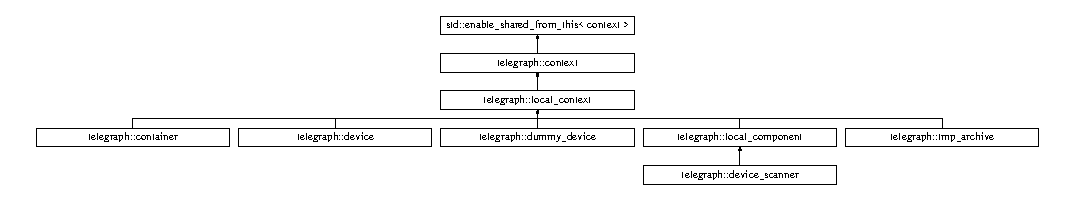
\includegraphics[height=2.258065cm]{classtelegraph_1_1context}
\end{center}
\end{figure}
\subsection*{Public Member Functions}
\begin{DoxyCompactItemize}
\item 
\hyperlink{classtelegraph_1_1context_ad57ca6ff5da9ad653c688e7be3c0bbdc}{context} (io\+::io\+\_\+context \&ioc, const \hyperlink{namespacetelegraph_a51ee91d7eaeef067f7ccac2b170e5d59}{uuid} \&\hyperlink{namespacetelegraph_a51ee91d7eaeef067f7ccac2b170e5d59}{uuid}, const std\+::string\+\_\+view \&name, const std\+::string\+\_\+view \&type, const \hyperlink{classtelegraph_1_1params}{params} \&p, bool headless)
\item 
constexpr io\+::io\+\_\+context \& \hyperlink{classtelegraph_1_1context_a5df9df51fb9fc54d69e4a7d43e66345a}{get\+\_\+executor} ()
\item 
virtual std\+::shared\+\_\+ptr$<$ \hyperlink{classtelegraph_1_1namespace__}{namespace\+\_\+} $>$ \hyperlink{classtelegraph_1_1context_a84d92cca54be9c4e885e2673480e45a1}{get\+\_\+namespace} ()=0
\item 
virtual std\+::shared\+\_\+ptr$<$ const \hyperlink{classtelegraph_1_1namespace__}{namespace\+\_\+} $>$ \hyperlink{classtelegraph_1_1context_a2f6c9ecc15cee66415828df9efa834a2}{get\+\_\+namespace} () const =0
\item 
const bool \hyperlink{classtelegraph_1_1context_a4cfaa125584e2f5ee5121c074bc024f1}{is\+\_\+headless} () const
\item 
const std\+::string \& \hyperlink{classtelegraph_1_1context_a56bd2af5bbfcdc234f6dd8df052585d7}{get\+\_\+name} () const
\item 
const std\+::string \& \hyperlink{classtelegraph_1_1context_a07d07a63d22454c2dc900c5cf749ce18}{get\+\_\+type} () const
\item 
const \hyperlink{classtelegraph_1_1params}{params} \& \hyperlink{classtelegraph_1_1context_ab8f2cf6a295d840f8011ff1b5533a1f8}{get\+\_\+params} () const
\item 
const \hyperlink{namespacetelegraph_a51ee91d7eaeef067f7ccac2b170e5d59}{uuid} \& \hyperlink{classtelegraph_1_1context_adfc55d7a2ba9d68c1f52abcbac7d74fd}{get\+\_\+uuid} () const
\item 
virtual \hyperlink{namespacetelegraph_ad071241508ea0f86c7de0686016f9ca9}{params\+\_\+stream\+\_\+ptr} \hyperlink{classtelegraph_1_1context_a6765d7fa22fe99b9a6723c511396b781}{request} (\hyperlink{structboost_1_1asio_1_1yield__ctx}{io\+::yield\+\_\+ctx} \&, const \hyperlink{classtelegraph_1_1params}{params} \&p)=0
\item 
virtual std\+::shared\+\_\+ptr$<$ \hyperlink{classtelegraph_1_1node}{node} $>$ \hyperlink{classtelegraph_1_1context_aa2c0321629f2d51c8bc5632e418b305f}{fetch} (\hyperlink{structboost_1_1asio_1_1yield__ctx}{io\+::yield\+\_\+ctx} \&ctx)=0
\item 
virtual \hyperlink{namespacetelegraph_a58641aa5b1a2cbdb0431916a87069f64}{subscription\+\_\+ptr} \hyperlink{classtelegraph_1_1context_a8db167973f187f707a4108e112683969}{subscribe} (\hyperlink{structboost_1_1asio_1_1yield__ctx}{io\+::yield\+\_\+ctx} \&ctx, const std\+::vector$<$ std\+::string\+\_\+view $>$ \&\hyperlink{classtelegraph_1_1variable}{variable}, float min\+\_\+interval, float max\+\_\+interval, float timeout)=0
\item 
virtual \hyperlink{namespacetelegraph_a58641aa5b1a2cbdb0431916a87069f64}{subscription\+\_\+ptr} \hyperlink{classtelegraph_1_1context_aec3b3b0d7210a86f2ea2f5067ef8e922}{subscribe} (\hyperlink{structboost_1_1asio_1_1yield__ctx}{io\+::yield\+\_\+ctx} \&ctx, const \hyperlink{classtelegraph_1_1variable}{variable} $\ast$v, float min\+\_\+interval, float max\+\_\+interval, float timeout)=0
\item 
virtual \hyperlink{classtelegraph_1_1value}{value} \hyperlink{classtelegraph_1_1context_a72da471eb635e5505b10d2f1103359ac}{call} (\hyperlink{structboost_1_1asio_1_1yield__ctx}{io\+::yield\+\_\+ctx} \&ctx, \hyperlink{classtelegraph_1_1action}{action} $\ast$a, \hyperlink{classtelegraph_1_1value}{value} v, float timeout)=0
\item 
virtual \hyperlink{classtelegraph_1_1value}{value} \hyperlink{classtelegraph_1_1context_a0798d49ea0874a870d4c980f6f09b6c2}{call} (\hyperlink{structboost_1_1asio_1_1yield__ctx}{io\+::yield\+\_\+ctx} \&ctx, const std\+::vector$<$ std\+::string\+\_\+view $>$ \&a, \hyperlink{classtelegraph_1_1value}{value} v, float timeout)=0
\item 
virtual bool \hyperlink{classtelegraph_1_1context_a6067b9a6f2590733c81f6a3b2ed9cba7}{write\+\_\+data} (\hyperlink{structboost_1_1asio_1_1yield__ctx}{io\+::yield\+\_\+ctx} \&yield, \hyperlink{classtelegraph_1_1variable}{variable} $\ast$v, const std\+::vector$<$ \hyperlink{classtelegraph_1_1data__point}{data\+\_\+point} $>$ \&data)=0
\item 
virtual bool \hyperlink{classtelegraph_1_1context_a1f600d6159df21dd2750b1c706ca3412}{write\+\_\+data} (\hyperlink{structboost_1_1asio_1_1yield__ctx}{io\+::yield\+\_\+ctx} \&yield, const std\+::vector$<$ std\+::string\+\_\+view $>$ \&var, const std\+::vector$<$ \hyperlink{classtelegraph_1_1data__point}{data\+\_\+point} $>$ \&data)=0
\item 
virtual \hyperlink{namespacetelegraph_a6ffe775ac48dca2a4013b53d692199c8}{data\+\_\+query\+\_\+ptr} \hyperlink{classtelegraph_1_1context_a301114c9b73194507ae58221566a3e57}{query\+\_\+data} (\hyperlink{structboost_1_1asio_1_1yield__ctx}{io\+::yield\+\_\+ctx} \&yield, const \hyperlink{classtelegraph_1_1variable}{variable} $\ast$v)=0
\item 
virtual \hyperlink{namespacetelegraph_a6ffe775ac48dca2a4013b53d692199c8}{data\+\_\+query\+\_\+ptr} \hyperlink{classtelegraph_1_1context_a34793623d2a2def580ad0b8710c74c6d}{query\+\_\+data} (\hyperlink{structboost_1_1asio_1_1yield__ctx}{io\+::yield\+\_\+ctx} \&yield, const std\+::vector$<$ std\+::string\+\_\+view $>$ \&v)=0
\item 
virtual void \hyperlink{classtelegraph_1_1context_a4017c1bcd9c84170a5cb612ae45d6fb4}{destroy} (\hyperlink{structboost_1_1asio_1_1yield__ctx}{io\+::yield\+\_\+ctx} \&yield)=0
\end{DoxyCompactItemize}
\subsection*{Public Attributes}
\begin{DoxyCompactItemize}
\item 
\hyperlink{classtelegraph_1_1signal}{signal} \hyperlink{classtelegraph_1_1context_aeae90cedad8326dcd9d6180d1058a10f}{destroyed}
\end{DoxyCompactItemize}
\subsection*{Protected Attributes}
\begin{DoxyCompactItemize}
\item 
io\+::io\+\_\+context \& \hyperlink{classtelegraph_1_1context_a51949d83373c67e0c9e1050127df30c1}{ioc\+\_\+}
\item 
const \hyperlink{namespacetelegraph_a51ee91d7eaeef067f7ccac2b170e5d59}{uuid} \hyperlink{classtelegraph_1_1context_a0bf1873b5a611776d48b3e854e9e3589}{uuid\+\_\+}
\item 
const bool \hyperlink{classtelegraph_1_1context_a5053f72fe2b58e264a0ce00de2727953}{headless\+\_\+}
\item 
const std\+::string \hyperlink{classtelegraph_1_1context_a19b7cc6a4c3cf53d79e07fc78573fc31}{name\+\_\+}
\item 
const std\+::string \hyperlink{classtelegraph_1_1context_af1cab34ed3278340157e25d828bb6c77}{type\+\_\+}
\item 
const \hyperlink{classtelegraph_1_1params}{params} \hyperlink{classtelegraph_1_1context_aa80ae462af488940258d71ccb6435b33}{params\+\_\+}
\end{DoxyCompactItemize}


\subsection{Constructor \& Destructor Documentation}
\mbox{\Hypertarget{classtelegraph_1_1context_ad57ca6ff5da9ad653c688e7be3c0bbdc}\label{classtelegraph_1_1context_ad57ca6ff5da9ad653c688e7be3c0bbdc}} 
\index{telegraph\+::context@{telegraph\+::context}!context@{context}}
\index{context@{context}!telegraph\+::context@{telegraph\+::context}}
\subsubsection{\texorpdfstring{context()}{context()}}
{\footnotesize\ttfamily telegraph\+::context\+::context (\begin{DoxyParamCaption}\item[{io\+::io\+\_\+context \&}]{ioc,  }\item[{const \hyperlink{namespacetelegraph_a51ee91d7eaeef067f7ccac2b170e5d59}{uuid} \&}]{uuid,  }\item[{const std\+::string\+\_\+view \&}]{name,  }\item[{const std\+::string\+\_\+view \&}]{type,  }\item[{const \hyperlink{classtelegraph_1_1params}{params} \&}]{p,  }\item[{bool}]{headless }\end{DoxyParamCaption})\hspace{0.3cm}{\ttfamily [inline]}}



\subsection{Member Function Documentation}
\mbox{\Hypertarget{classtelegraph_1_1context_a72da471eb635e5505b10d2f1103359ac}\label{classtelegraph_1_1context_a72da471eb635e5505b10d2f1103359ac}} 
\index{telegraph\+::context@{telegraph\+::context}!call@{call}}
\index{call@{call}!telegraph\+::context@{telegraph\+::context}}
\subsubsection{\texorpdfstring{call()}{call()}\hspace{0.1cm}{\footnotesize\ttfamily [1/2]}}
{\footnotesize\ttfamily virtual \hyperlink{classtelegraph_1_1value}{value} telegraph\+::context\+::call (\begin{DoxyParamCaption}\item[{\hyperlink{structboost_1_1asio_1_1yield__ctx}{io\+::yield\+\_\+ctx} \&}]{ctx,  }\item[{\hyperlink{classtelegraph_1_1action}{action} $\ast$}]{a,  }\item[{\hyperlink{classtelegraph_1_1value}{value}}]{v,  }\item[{float}]{timeout }\end{DoxyParamCaption})\hspace{0.3cm}{\ttfamily [pure virtual]}}



Implemented in \hyperlink{classtelegraph_1_1tmp__archive_a9edb8a731ef989f40ae06e4b6c63c0be}{telegraph\+::tmp\+\_\+archive}, \hyperlink{classtelegraph_1_1local__component_af4d74d161754055d3f811bfe95a59f26}{telegraph\+::local\+\_\+component}, \hyperlink{classtelegraph_1_1device_ac6558ddeed4799f4d69428863363a1e6}{telegraph\+::device}, \hyperlink{classtelegraph_1_1container_a499649499d61f07dbe44bbec933414a0}{telegraph\+::container}, and \hyperlink{classtelegraph_1_1dummy__device_af2e3be5731809d7693cb6a4607e5e3f6}{telegraph\+::dummy\+\_\+device}.

\mbox{\Hypertarget{classtelegraph_1_1context_a0798d49ea0874a870d4c980f6f09b6c2}\label{classtelegraph_1_1context_a0798d49ea0874a870d4c980f6f09b6c2}} 
\index{telegraph\+::context@{telegraph\+::context}!call@{call}}
\index{call@{call}!telegraph\+::context@{telegraph\+::context}}
\subsubsection{\texorpdfstring{call()}{call()}\hspace{0.1cm}{\footnotesize\ttfamily [2/2]}}
{\footnotesize\ttfamily virtual \hyperlink{classtelegraph_1_1value}{value} telegraph\+::context\+::call (\begin{DoxyParamCaption}\item[{\hyperlink{structboost_1_1asio_1_1yield__ctx}{io\+::yield\+\_\+ctx} \&}]{ctx,  }\item[{const std\+::vector$<$ std\+::string\+\_\+view $>$ \&}]{a,  }\item[{\hyperlink{classtelegraph_1_1value}{value}}]{v,  }\item[{float}]{timeout }\end{DoxyParamCaption})\hspace{0.3cm}{\ttfamily [pure virtual]}}



Implemented in \hyperlink{classtelegraph_1_1tmp__archive_a1ccf8c90f14b36f3a09a501e0931e42e}{telegraph\+::tmp\+\_\+archive}, \hyperlink{classtelegraph_1_1local__component_a6fa6fbf49a0d77a8da54b4a77b578edd}{telegraph\+::local\+\_\+component}, \hyperlink{classtelegraph_1_1device_a581368ab8f35ef72db17d2e330ded068}{telegraph\+::device}, \hyperlink{classtelegraph_1_1container_a83d26f574b7f75655be9752147e30dce}{telegraph\+::container}, and \hyperlink{classtelegraph_1_1dummy__device_ab037df44b352953369760dd6071d84b5}{telegraph\+::dummy\+\_\+device}.

\mbox{\Hypertarget{classtelegraph_1_1context_a4017c1bcd9c84170a5cb612ae45d6fb4}\label{classtelegraph_1_1context_a4017c1bcd9c84170a5cb612ae45d6fb4}} 
\index{telegraph\+::context@{telegraph\+::context}!destroy@{destroy}}
\index{destroy@{destroy}!telegraph\+::context@{telegraph\+::context}}
\subsubsection{\texorpdfstring{destroy()}{destroy()}}
{\footnotesize\ttfamily virtual void telegraph\+::context\+::destroy (\begin{DoxyParamCaption}\item[{\hyperlink{structboost_1_1asio_1_1yield__ctx}{io\+::yield\+\_\+ctx} \&}]{yield }\end{DoxyParamCaption})\hspace{0.3cm}{\ttfamily [pure virtual]}}



Implemented in \hyperlink{classtelegraph_1_1device_a8d619b64e89b2ae933b282dc05956d37}{telegraph\+::device}, and \hyperlink{classtelegraph_1_1local__context_a301da16810636030a5098e4838587a99}{telegraph\+::local\+\_\+context}.

\mbox{\Hypertarget{classtelegraph_1_1context_aa2c0321629f2d51c8bc5632e418b305f}\label{classtelegraph_1_1context_aa2c0321629f2d51c8bc5632e418b305f}} 
\index{telegraph\+::context@{telegraph\+::context}!fetch@{fetch}}
\index{fetch@{fetch}!telegraph\+::context@{telegraph\+::context}}
\subsubsection{\texorpdfstring{fetch()}{fetch()}}
{\footnotesize\ttfamily virtual std\+::shared\+\_\+ptr$<$\hyperlink{classtelegraph_1_1node}{node}$>$ telegraph\+::context\+::fetch (\begin{DoxyParamCaption}\item[{\hyperlink{structboost_1_1asio_1_1yield__ctx}{io\+::yield\+\_\+ctx} \&}]{ctx }\end{DoxyParamCaption})\hspace{0.3cm}{\ttfamily [pure virtual]}}



Implemented in \hyperlink{classtelegraph_1_1local__component_abbeb3b12dc95e19e1a2972e9a374fd33}{telegraph\+::local\+\_\+component}, and \hyperlink{classtelegraph_1_1local__context_aefadafdf25e6f6ba23c4b332872836e2}{telegraph\+::local\+\_\+context}.

\mbox{\Hypertarget{classtelegraph_1_1context_a5df9df51fb9fc54d69e4a7d43e66345a}\label{classtelegraph_1_1context_a5df9df51fb9fc54d69e4a7d43e66345a}} 
\index{telegraph\+::context@{telegraph\+::context}!get\+\_\+executor@{get\+\_\+executor}}
\index{get\+\_\+executor@{get\+\_\+executor}!telegraph\+::context@{telegraph\+::context}}
\subsubsection{\texorpdfstring{get\+\_\+executor()}{get\_executor()}}
{\footnotesize\ttfamily constexpr io\+::io\+\_\+context\& telegraph\+::context\+::get\+\_\+executor (\begin{DoxyParamCaption}{ }\end{DoxyParamCaption})\hspace{0.3cm}{\ttfamily [inline]}}

\mbox{\Hypertarget{classtelegraph_1_1context_a56bd2af5bbfcdc234f6dd8df052585d7}\label{classtelegraph_1_1context_a56bd2af5bbfcdc234f6dd8df052585d7}} 
\index{telegraph\+::context@{telegraph\+::context}!get\+\_\+name@{get\+\_\+name}}
\index{get\+\_\+name@{get\+\_\+name}!telegraph\+::context@{telegraph\+::context}}
\subsubsection{\texorpdfstring{get\+\_\+name()}{get\_name()}}
{\footnotesize\ttfamily const std\+::string\& telegraph\+::context\+::get\+\_\+name (\begin{DoxyParamCaption}{ }\end{DoxyParamCaption}) const\hspace{0.3cm}{\ttfamily [inline]}}

\mbox{\Hypertarget{classtelegraph_1_1context_a84d92cca54be9c4e885e2673480e45a1}\label{classtelegraph_1_1context_a84d92cca54be9c4e885e2673480e45a1}} 
\index{telegraph\+::context@{telegraph\+::context}!get\+\_\+namespace@{get\+\_\+namespace}}
\index{get\+\_\+namespace@{get\+\_\+namespace}!telegraph\+::context@{telegraph\+::context}}
\subsubsection{\texorpdfstring{get\+\_\+namespace()}{get\_namespace()}\hspace{0.1cm}{\footnotesize\ttfamily [1/2]}}
{\footnotesize\ttfamily virtual std\+::shared\+\_\+ptr$<$\hyperlink{classtelegraph_1_1namespace__}{namespace\+\_\+}$>$ telegraph\+::context\+::get\+\_\+namespace (\begin{DoxyParamCaption}{ }\end{DoxyParamCaption})\hspace{0.3cm}{\ttfamily [pure virtual]}}



Implemented in \hyperlink{classtelegraph_1_1local__context_a71a19090a93c3193615e61940fba918a}{telegraph\+::local\+\_\+context}.

\mbox{\Hypertarget{classtelegraph_1_1context_a2f6c9ecc15cee66415828df9efa834a2}\label{classtelegraph_1_1context_a2f6c9ecc15cee66415828df9efa834a2}} 
\index{telegraph\+::context@{telegraph\+::context}!get\+\_\+namespace@{get\+\_\+namespace}}
\index{get\+\_\+namespace@{get\+\_\+namespace}!telegraph\+::context@{telegraph\+::context}}
\subsubsection{\texorpdfstring{get\+\_\+namespace()}{get\_namespace()}\hspace{0.1cm}{\footnotesize\ttfamily [2/2]}}
{\footnotesize\ttfamily virtual std\+::shared\+\_\+ptr$<$const \hyperlink{classtelegraph_1_1namespace__}{namespace\+\_\+}$>$ telegraph\+::context\+::get\+\_\+namespace (\begin{DoxyParamCaption}{ }\end{DoxyParamCaption}) const\hspace{0.3cm}{\ttfamily [pure virtual]}}



Implemented in \hyperlink{classtelegraph_1_1local__context_aba1ff115df4b54bae75ea41580ba32b5}{telegraph\+::local\+\_\+context}.

\mbox{\Hypertarget{classtelegraph_1_1context_ab8f2cf6a295d840f8011ff1b5533a1f8}\label{classtelegraph_1_1context_ab8f2cf6a295d840f8011ff1b5533a1f8}} 
\index{telegraph\+::context@{telegraph\+::context}!get\+\_\+params@{get\+\_\+params}}
\index{get\+\_\+params@{get\+\_\+params}!telegraph\+::context@{telegraph\+::context}}
\subsubsection{\texorpdfstring{get\+\_\+params()}{get\_params()}}
{\footnotesize\ttfamily const \hyperlink{classtelegraph_1_1params}{params}\& telegraph\+::context\+::get\+\_\+params (\begin{DoxyParamCaption}{ }\end{DoxyParamCaption}) const\hspace{0.3cm}{\ttfamily [inline]}}

\mbox{\Hypertarget{classtelegraph_1_1context_a07d07a63d22454c2dc900c5cf749ce18}\label{classtelegraph_1_1context_a07d07a63d22454c2dc900c5cf749ce18}} 
\index{telegraph\+::context@{telegraph\+::context}!get\+\_\+type@{get\+\_\+type}}
\index{get\+\_\+type@{get\+\_\+type}!telegraph\+::context@{telegraph\+::context}}
\subsubsection{\texorpdfstring{get\+\_\+type()}{get\_type()}}
{\footnotesize\ttfamily const std\+::string\& telegraph\+::context\+::get\+\_\+type (\begin{DoxyParamCaption}{ }\end{DoxyParamCaption}) const\hspace{0.3cm}{\ttfamily [inline]}}

\mbox{\Hypertarget{classtelegraph_1_1context_adfc55d7a2ba9d68c1f52abcbac7d74fd}\label{classtelegraph_1_1context_adfc55d7a2ba9d68c1f52abcbac7d74fd}} 
\index{telegraph\+::context@{telegraph\+::context}!get\+\_\+uuid@{get\+\_\+uuid}}
\index{get\+\_\+uuid@{get\+\_\+uuid}!telegraph\+::context@{telegraph\+::context}}
\subsubsection{\texorpdfstring{get\+\_\+uuid()}{get\_uuid()}}
{\footnotesize\ttfamily const \hyperlink{namespacetelegraph_a51ee91d7eaeef067f7ccac2b170e5d59}{uuid}\& telegraph\+::context\+::get\+\_\+uuid (\begin{DoxyParamCaption}{ }\end{DoxyParamCaption}) const\hspace{0.3cm}{\ttfamily [inline]}}

\mbox{\Hypertarget{classtelegraph_1_1context_a4cfaa125584e2f5ee5121c074bc024f1}\label{classtelegraph_1_1context_a4cfaa125584e2f5ee5121c074bc024f1}} 
\index{telegraph\+::context@{telegraph\+::context}!is\+\_\+headless@{is\+\_\+headless}}
\index{is\+\_\+headless@{is\+\_\+headless}!telegraph\+::context@{telegraph\+::context}}
\subsubsection{\texorpdfstring{is\+\_\+headless()}{is\_headless()}}
{\footnotesize\ttfamily const bool telegraph\+::context\+::is\+\_\+headless (\begin{DoxyParamCaption}{ }\end{DoxyParamCaption}) const\hspace{0.3cm}{\ttfamily [inline]}}

\mbox{\Hypertarget{classtelegraph_1_1context_a301114c9b73194507ae58221566a3e57}\label{classtelegraph_1_1context_a301114c9b73194507ae58221566a3e57}} 
\index{telegraph\+::context@{telegraph\+::context}!query\+\_\+data@{query\+\_\+data}}
\index{query\+\_\+data@{query\+\_\+data}!telegraph\+::context@{telegraph\+::context}}
\subsubsection{\texorpdfstring{query\+\_\+data()}{query\_data()}\hspace{0.1cm}{\footnotesize\ttfamily [1/2]}}
{\footnotesize\ttfamily virtual \hyperlink{namespacetelegraph_a6ffe775ac48dca2a4013b53d692199c8}{data\+\_\+query\+\_\+ptr} telegraph\+::context\+::query\+\_\+data (\begin{DoxyParamCaption}\item[{\hyperlink{structboost_1_1asio_1_1yield__ctx}{io\+::yield\+\_\+ctx} \&}]{yield,  }\item[{const \hyperlink{classtelegraph_1_1variable}{variable} $\ast$}]{v }\end{DoxyParamCaption})\hspace{0.3cm}{\ttfamily [pure virtual]}}



Implemented in \hyperlink{classtelegraph_1_1local__component_a4410ca44a41de1c139273efd31f281c4}{telegraph\+::local\+\_\+component}, \hyperlink{classtelegraph_1_1device_a4c46c7e98bf5a573a9966fd2cc199021}{telegraph\+::device}, \hyperlink{classtelegraph_1_1dummy__device_a23b7704d488ca5e9ac732256621e8137}{telegraph\+::dummy\+\_\+device}, \hyperlink{classtelegraph_1_1container_a1a9849e53091061da81e7c1a73502e47}{telegraph\+::container}, and \hyperlink{classtelegraph_1_1tmp__archive_a7f2d18d2a4c9a7fd65d9752c8f4ce4d5}{telegraph\+::tmp\+\_\+archive}.

\mbox{\Hypertarget{classtelegraph_1_1context_a34793623d2a2def580ad0b8710c74c6d}\label{classtelegraph_1_1context_a34793623d2a2def580ad0b8710c74c6d}} 
\index{telegraph\+::context@{telegraph\+::context}!query\+\_\+data@{query\+\_\+data}}
\index{query\+\_\+data@{query\+\_\+data}!telegraph\+::context@{telegraph\+::context}}
\subsubsection{\texorpdfstring{query\+\_\+data()}{query\_data()}\hspace{0.1cm}{\footnotesize\ttfamily [2/2]}}
{\footnotesize\ttfamily virtual \hyperlink{namespacetelegraph_a6ffe775ac48dca2a4013b53d692199c8}{data\+\_\+query\+\_\+ptr} telegraph\+::context\+::query\+\_\+data (\begin{DoxyParamCaption}\item[{\hyperlink{structboost_1_1asio_1_1yield__ctx}{io\+::yield\+\_\+ctx} \&}]{yield,  }\item[{const std\+::vector$<$ std\+::string\+\_\+view $>$ \&}]{v }\end{DoxyParamCaption})\hspace{0.3cm}{\ttfamily [pure virtual]}}



Implemented in \hyperlink{classtelegraph_1_1local__component_ad8c3abb4f9e6ab31b0590beac901eec5}{telegraph\+::local\+\_\+component}, \hyperlink{classtelegraph_1_1device_a9a5ef799aadf591a355cc1e50442d762}{telegraph\+::device}, \hyperlink{classtelegraph_1_1tmp__archive_a8a860d67e3733e2eee7a8315942450e5}{telegraph\+::tmp\+\_\+archive}, \hyperlink{classtelegraph_1_1dummy__device_ae7820cd8f1d5683ccc90b7256e88a735}{telegraph\+::dummy\+\_\+device}, and \hyperlink{classtelegraph_1_1container_aca8b0b22be3cde48f0bc5f3fa79b29da}{telegraph\+::container}.

\mbox{\Hypertarget{classtelegraph_1_1context_a6765d7fa22fe99b9a6723c511396b781}\label{classtelegraph_1_1context_a6765d7fa22fe99b9a6723c511396b781}} 
\index{telegraph\+::context@{telegraph\+::context}!request@{request}}
\index{request@{request}!telegraph\+::context@{telegraph\+::context}}
\subsubsection{\texorpdfstring{request()}{request()}}
{\footnotesize\ttfamily virtual \hyperlink{namespacetelegraph_ad071241508ea0f86c7de0686016f9ca9}{params\+\_\+stream\+\_\+ptr} telegraph\+::context\+::request (\begin{DoxyParamCaption}\item[{\hyperlink{structboost_1_1asio_1_1yield__ctx}{io\+::yield\+\_\+ctx} \&}]{,  }\item[{const \hyperlink{classtelegraph_1_1params}{params} \&}]{p }\end{DoxyParamCaption})\hspace{0.3cm}{\ttfamily [pure virtual]}}



Implemented in \hyperlink{classtelegraph_1_1device__scanner_a5873278cb04e50896c3f125639df4c73}{telegraph\+::device\+\_\+scanner}, \hyperlink{classtelegraph_1_1device_a9e5042e4640035b28dd9de780d7326df}{telegraph\+::device}, \hyperlink{classtelegraph_1_1tmp__archive_a688a661b85092244e5634f9c3e380f94}{telegraph\+::tmp\+\_\+archive}, \hyperlink{classtelegraph_1_1container_ade9ce299ee72554a84c1a71f0ad37915}{telegraph\+::container}, and \hyperlink{classtelegraph_1_1dummy__device_a46d728506b36e9e8b5b6939eb6aefe12}{telegraph\+::dummy\+\_\+device}.

\mbox{\Hypertarget{classtelegraph_1_1context_a8db167973f187f707a4108e112683969}\label{classtelegraph_1_1context_a8db167973f187f707a4108e112683969}} 
\index{telegraph\+::context@{telegraph\+::context}!subscribe@{subscribe}}
\index{subscribe@{subscribe}!telegraph\+::context@{telegraph\+::context}}
\subsubsection{\texorpdfstring{subscribe()}{subscribe()}\hspace{0.1cm}{\footnotesize\ttfamily [1/2]}}
{\footnotesize\ttfamily virtual \hyperlink{namespacetelegraph_a58641aa5b1a2cbdb0431916a87069f64}{subscription\+\_\+ptr} telegraph\+::context\+::subscribe (\begin{DoxyParamCaption}\item[{\hyperlink{structboost_1_1asio_1_1yield__ctx}{io\+::yield\+\_\+ctx} \&}]{ctx,  }\item[{const std\+::vector$<$ std\+::string\+\_\+view $>$ \&}]{variable,  }\item[{float}]{min\+\_\+interval,  }\item[{float}]{max\+\_\+interval,  }\item[{float}]{timeout }\end{DoxyParamCaption})\hspace{0.3cm}{\ttfamily [pure virtual]}}



Implemented in \hyperlink{classtelegraph_1_1tmp__archive_a9cf4be673f860b875b085c1ecac913ff}{telegraph\+::tmp\+\_\+archive}, \hyperlink{classtelegraph_1_1local__component_a53aa0199bd938578a6400cfd3a19c86f}{telegraph\+::local\+\_\+component}, \hyperlink{classtelegraph_1_1device_aedf52d2dbb133e2b71958c116671b9df}{telegraph\+::device}, \hyperlink{classtelegraph_1_1container_ae1ae26a08bf3d367bbc13020623780b2}{telegraph\+::container}, and \hyperlink{classtelegraph_1_1dummy__device_a8996ac06dfc98de11c3d156b4a0a2caf}{telegraph\+::dummy\+\_\+device}.

\mbox{\Hypertarget{classtelegraph_1_1context_aec3b3b0d7210a86f2ea2f5067ef8e922}\label{classtelegraph_1_1context_aec3b3b0d7210a86f2ea2f5067ef8e922}} 
\index{telegraph\+::context@{telegraph\+::context}!subscribe@{subscribe}}
\index{subscribe@{subscribe}!telegraph\+::context@{telegraph\+::context}}
\subsubsection{\texorpdfstring{subscribe()}{subscribe()}\hspace{0.1cm}{\footnotesize\ttfamily [2/2]}}
{\footnotesize\ttfamily virtual \hyperlink{namespacetelegraph_a58641aa5b1a2cbdb0431916a87069f64}{subscription\+\_\+ptr} telegraph\+::context\+::subscribe (\begin{DoxyParamCaption}\item[{\hyperlink{structboost_1_1asio_1_1yield__ctx}{io\+::yield\+\_\+ctx} \&}]{ctx,  }\item[{const \hyperlink{classtelegraph_1_1variable}{variable} $\ast$}]{v,  }\item[{float}]{min\+\_\+interval,  }\item[{float}]{max\+\_\+interval,  }\item[{float}]{timeout }\end{DoxyParamCaption})\hspace{0.3cm}{\ttfamily [pure virtual]}}



Implemented in \hyperlink{classtelegraph_1_1local__component_a5a2282f1cf80dce32ed26e37c956d5c4}{telegraph\+::local\+\_\+component}, \hyperlink{classtelegraph_1_1tmp__archive_a10adc383103f4183e0a37485a5406cf1}{telegraph\+::tmp\+\_\+archive}, \hyperlink{classtelegraph_1_1device_ab0117f6015f904afae72d6ab90c8ad95}{telegraph\+::device}, \hyperlink{classtelegraph_1_1container_aa11f4e622d784b566a032c05f2019264}{telegraph\+::container}, and \hyperlink{classtelegraph_1_1dummy__device_a06470ed069c481e8199dce9387448c8b}{telegraph\+::dummy\+\_\+device}.

\mbox{\Hypertarget{classtelegraph_1_1context_a6067b9a6f2590733c81f6a3b2ed9cba7}\label{classtelegraph_1_1context_a6067b9a6f2590733c81f6a3b2ed9cba7}} 
\index{telegraph\+::context@{telegraph\+::context}!write\+\_\+data@{write\+\_\+data}}
\index{write\+\_\+data@{write\+\_\+data}!telegraph\+::context@{telegraph\+::context}}
\subsubsection{\texorpdfstring{write\+\_\+data()}{write\_data()}\hspace{0.1cm}{\footnotesize\ttfamily [1/2]}}
{\footnotesize\ttfamily virtual bool telegraph\+::context\+::write\+\_\+data (\begin{DoxyParamCaption}\item[{\hyperlink{structboost_1_1asio_1_1yield__ctx}{io\+::yield\+\_\+ctx} \&}]{yield,  }\item[{\hyperlink{classtelegraph_1_1variable}{variable} $\ast$}]{v,  }\item[{const std\+::vector$<$ \hyperlink{classtelegraph_1_1data__point}{data\+\_\+point} $>$ \&}]{data }\end{DoxyParamCaption})\hspace{0.3cm}{\ttfamily [pure virtual]}}



Implemented in \hyperlink{classtelegraph_1_1local__component_ac546cfea4802ef3ca125c5dc183adf6c}{telegraph\+::local\+\_\+component}, \hyperlink{classtelegraph_1_1device_a60150e55bc6fb63d27252051caf462db}{telegraph\+::device}, \hyperlink{classtelegraph_1_1dummy__device_a162f8f7a02c2907693ecf86662f6ffe1}{telegraph\+::dummy\+\_\+device}, \hyperlink{classtelegraph_1_1container_aad8390913b2961a2270e6d4065deb59b}{telegraph\+::container}, and \hyperlink{classtelegraph_1_1tmp__archive_ae1838ff3fc3f1cd0eab31535a2f2e974}{telegraph\+::tmp\+\_\+archive}.

\mbox{\Hypertarget{classtelegraph_1_1context_a1f600d6159df21dd2750b1c706ca3412}\label{classtelegraph_1_1context_a1f600d6159df21dd2750b1c706ca3412}} 
\index{telegraph\+::context@{telegraph\+::context}!write\+\_\+data@{write\+\_\+data}}
\index{write\+\_\+data@{write\+\_\+data}!telegraph\+::context@{telegraph\+::context}}
\subsubsection{\texorpdfstring{write\+\_\+data()}{write\_data()}\hspace{0.1cm}{\footnotesize\ttfamily [2/2]}}
{\footnotesize\ttfamily virtual bool telegraph\+::context\+::write\+\_\+data (\begin{DoxyParamCaption}\item[{\hyperlink{structboost_1_1asio_1_1yield__ctx}{io\+::yield\+\_\+ctx} \&}]{yield,  }\item[{const std\+::vector$<$ std\+::string\+\_\+view $>$ \&}]{var,  }\item[{const std\+::vector$<$ \hyperlink{classtelegraph_1_1data__point}{data\+\_\+point} $>$ \&}]{data }\end{DoxyParamCaption})\hspace{0.3cm}{\ttfamily [pure virtual]}}



Implemented in \hyperlink{classtelegraph_1_1local__component_a572a4116130a4b7ad270701eba2af0e7}{telegraph\+::local\+\_\+component}, \hyperlink{classtelegraph_1_1device_aaedca7b20bc36f8439d5afccbcaf1304}{telegraph\+::device}, \hyperlink{classtelegraph_1_1dummy__device_a2d18fd0ec74a6d4bb76f789135403f19}{telegraph\+::dummy\+\_\+device}, \hyperlink{classtelegraph_1_1container_a6c608535adf0fee7783f6684ab4b69c8}{telegraph\+::container}, and \hyperlink{classtelegraph_1_1tmp__archive_a228c2c681beb749268d09cd83d594246}{telegraph\+::tmp\+\_\+archive}.



\subsection{Member Data Documentation}
\mbox{\Hypertarget{classtelegraph_1_1context_aeae90cedad8326dcd9d6180d1058a10f}\label{classtelegraph_1_1context_aeae90cedad8326dcd9d6180d1058a10f}} 
\index{telegraph\+::context@{telegraph\+::context}!destroyed@{destroyed}}
\index{destroyed@{destroyed}!telegraph\+::context@{telegraph\+::context}}
\subsubsection{\texorpdfstring{destroyed}{destroyed}}
{\footnotesize\ttfamily \hyperlink{classtelegraph_1_1signal}{signal} telegraph\+::context\+::destroyed}

\mbox{\Hypertarget{classtelegraph_1_1context_a5053f72fe2b58e264a0ce00de2727953}\label{classtelegraph_1_1context_a5053f72fe2b58e264a0ce00de2727953}} 
\index{telegraph\+::context@{telegraph\+::context}!headless\+\_\+@{headless\+\_\+}}
\index{headless\+\_\+@{headless\+\_\+}!telegraph\+::context@{telegraph\+::context}}
\subsubsection{\texorpdfstring{headless\+\_\+}{headless\_}}
{\footnotesize\ttfamily const bool telegraph\+::context\+::headless\+\_\+\hspace{0.3cm}{\ttfamily [protected]}}

\mbox{\Hypertarget{classtelegraph_1_1context_a51949d83373c67e0c9e1050127df30c1}\label{classtelegraph_1_1context_a51949d83373c67e0c9e1050127df30c1}} 
\index{telegraph\+::context@{telegraph\+::context}!ioc\+\_\+@{ioc\+\_\+}}
\index{ioc\+\_\+@{ioc\+\_\+}!telegraph\+::context@{telegraph\+::context}}
\subsubsection{\texorpdfstring{ioc\+\_\+}{ioc\_}}
{\footnotesize\ttfamily io\+::io\+\_\+context\& telegraph\+::context\+::ioc\+\_\+\hspace{0.3cm}{\ttfamily [protected]}}

\mbox{\Hypertarget{classtelegraph_1_1context_a19b7cc6a4c3cf53d79e07fc78573fc31}\label{classtelegraph_1_1context_a19b7cc6a4c3cf53d79e07fc78573fc31}} 
\index{telegraph\+::context@{telegraph\+::context}!name\+\_\+@{name\+\_\+}}
\index{name\+\_\+@{name\+\_\+}!telegraph\+::context@{telegraph\+::context}}
\subsubsection{\texorpdfstring{name\+\_\+}{name\_}}
{\footnotesize\ttfamily const std\+::string telegraph\+::context\+::name\+\_\+\hspace{0.3cm}{\ttfamily [protected]}}

\mbox{\Hypertarget{classtelegraph_1_1context_aa80ae462af488940258d71ccb6435b33}\label{classtelegraph_1_1context_aa80ae462af488940258d71ccb6435b33}} 
\index{telegraph\+::context@{telegraph\+::context}!params\+\_\+@{params\+\_\+}}
\index{params\+\_\+@{params\+\_\+}!telegraph\+::context@{telegraph\+::context}}
\subsubsection{\texorpdfstring{params\+\_\+}{params\_}}
{\footnotesize\ttfamily const \hyperlink{classtelegraph_1_1params}{params} telegraph\+::context\+::params\+\_\+\hspace{0.3cm}{\ttfamily [protected]}}

\mbox{\Hypertarget{classtelegraph_1_1context_af1cab34ed3278340157e25d828bb6c77}\label{classtelegraph_1_1context_af1cab34ed3278340157e25d828bb6c77}} 
\index{telegraph\+::context@{telegraph\+::context}!type\+\_\+@{type\+\_\+}}
\index{type\+\_\+@{type\+\_\+}!telegraph\+::context@{telegraph\+::context}}
\subsubsection{\texorpdfstring{type\+\_\+}{type\_}}
{\footnotesize\ttfamily const std\+::string telegraph\+::context\+::type\+\_\+\hspace{0.3cm}{\ttfamily [protected]}}

\mbox{\Hypertarget{classtelegraph_1_1context_a0bf1873b5a611776d48b3e854e9e3589}\label{classtelegraph_1_1context_a0bf1873b5a611776d48b3e854e9e3589}} 
\index{telegraph\+::context@{telegraph\+::context}!uuid\+\_\+@{uuid\+\_\+}}
\index{uuid\+\_\+@{uuid\+\_\+}!telegraph\+::context@{telegraph\+::context}}
\subsubsection{\texorpdfstring{uuid\+\_\+}{uuid\_}}
{\footnotesize\ttfamily const \hyperlink{namespacetelegraph_a51ee91d7eaeef067f7ccac2b170e5d59}{uuid} telegraph\+::context\+::uuid\+\_\+\hspace{0.3cm}{\ttfamily [protected]}}



The documentation for this class was generated from the following file\+:\begin{DoxyCompactItemize}
\item 
\hyperlink{common_2namespace_8hpp}{common/namespace.\+hpp}\end{DoxyCompactItemize}

\hypertarget{structtelegen_1_1coroutine}{}\section{telegen\+:\+:coroutine Struct Reference}
\label{structtelegen_1_1coroutine}\index{telegen\+::coroutine@{telegen\+::coroutine}}


{\ttfamily \#include $<$coroutine.\+hpp$>$}

Inheritance diagram for telegen\+:\+:coroutine\+:\begin{figure}[H]
\begin{center}
\leavevmode
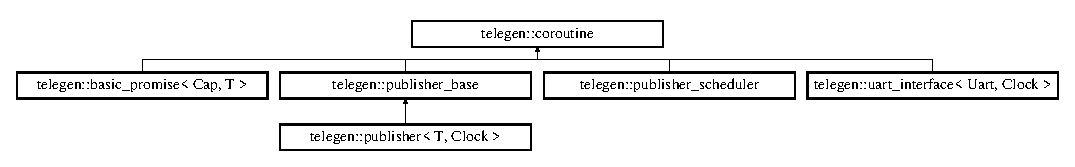
\includegraphics[height=1.794872cm]{structtelegen_1_1coroutine}
\end{center}
\end{figure}
\subsection*{Classes}
\begin{DoxyCompactItemize}
\item 
class \hyperlink{classtelegen_1_1coroutine_1_1ref}{ref}
\end{DoxyCompactItemize}
\subsection*{Public Member Functions}
\begin{DoxyCompactItemize}
\item 
constexpr \hyperlink{structtelegen_1_1coroutine_ac13b85fb7d6b08c684c69f1109c2f947}{coroutine} ()
\item 
virtual constexpr void \hyperlink{structtelegen_1_1coroutine_a345d1cc0fd5bd8d126022958d4f17d3b}{reset} ()
\item 
constexpr void \hyperlink{structtelegen_1_1coroutine_a335f75302785f4ee9d8073caf8cfc60b}{finish} ()
\item 
constexpr bool \hyperlink{structtelegen_1_1coroutine_a4e807c9f48ccfd7fd64a0b6ef2024da0}{is\+\_\+finished} ()
\item 
void \hyperlink{structtelegen_1_1coroutine_a48b19e2ca54c0a7b63fe5c5f19620bcb}{run} ()
\item 
virtual void \hyperlink{structtelegen_1_1coroutine_a2a7408a5b9474af3e59128934e3a5c00}{resume} ()=0
\end{DoxyCompactItemize}
\subsection*{Friends}
\begin{DoxyCompactItemize}
\item 
class \hyperlink{structtelegen_1_1coroutine_aa3d603af636458056061ae4b08fe9c18}{ref}
\end{DoxyCompactItemize}


\subsection{Constructor \& Destructor Documentation}
\mbox{\Hypertarget{structtelegen_1_1coroutine_ac13b85fb7d6b08c684c69f1109c2f947}\label{structtelegen_1_1coroutine_ac13b85fb7d6b08c684c69f1109c2f947}} 
\index{telegen\+::coroutine@{telegen\+::coroutine}!coroutine@{coroutine}}
\index{coroutine@{coroutine}!telegen\+::coroutine@{telegen\+::coroutine}}
\subsubsection{\texorpdfstring{coroutine()}{coroutine()}}
{\footnotesize\ttfamily constexpr telegen\+::coroutine\+::coroutine (\begin{DoxyParamCaption}{ }\end{DoxyParamCaption})\hspace{0.3cm}{\ttfamily [inline]}}



\subsection{Member Function Documentation}
\mbox{\Hypertarget{structtelegen_1_1coroutine_a335f75302785f4ee9d8073caf8cfc60b}\label{structtelegen_1_1coroutine_a335f75302785f4ee9d8073caf8cfc60b}} 
\index{telegen\+::coroutine@{telegen\+::coroutine}!finish@{finish}}
\index{finish@{finish}!telegen\+::coroutine@{telegen\+::coroutine}}
\subsubsection{\texorpdfstring{finish()}{finish()}}
{\footnotesize\ttfamily constexpr void telegen\+::coroutine\+::finish (\begin{DoxyParamCaption}{ }\end{DoxyParamCaption})\hspace{0.3cm}{\ttfamily [inline]}}

\mbox{\Hypertarget{structtelegen_1_1coroutine_a4e807c9f48ccfd7fd64a0b6ef2024da0}\label{structtelegen_1_1coroutine_a4e807c9f48ccfd7fd64a0b6ef2024da0}} 
\index{telegen\+::coroutine@{telegen\+::coroutine}!is\+\_\+finished@{is\+\_\+finished}}
\index{is\+\_\+finished@{is\+\_\+finished}!telegen\+::coroutine@{telegen\+::coroutine}}
\subsubsection{\texorpdfstring{is\+\_\+finished()}{is\_finished()}}
{\footnotesize\ttfamily constexpr bool telegen\+::coroutine\+::is\+\_\+finished (\begin{DoxyParamCaption}{ }\end{DoxyParamCaption})\hspace{0.3cm}{\ttfamily [inline]}}

\mbox{\Hypertarget{structtelegen_1_1coroutine_a345d1cc0fd5bd8d126022958d4f17d3b}\label{structtelegen_1_1coroutine_a345d1cc0fd5bd8d126022958d4f17d3b}} 
\index{telegen\+::coroutine@{telegen\+::coroutine}!reset@{reset}}
\index{reset@{reset}!telegen\+::coroutine@{telegen\+::coroutine}}
\subsubsection{\texorpdfstring{reset()}{reset()}}
{\footnotesize\ttfamily virtual constexpr void telegen\+::coroutine\+::reset (\begin{DoxyParamCaption}{ }\end{DoxyParamCaption})\hspace{0.3cm}{\ttfamily [inline]}, {\ttfamily [virtual]}}

\mbox{\Hypertarget{structtelegen_1_1coroutine_a2a7408a5b9474af3e59128934e3a5c00}\label{structtelegen_1_1coroutine_a2a7408a5b9474af3e59128934e3a5c00}} 
\index{telegen\+::coroutine@{telegen\+::coroutine}!resume@{resume}}
\index{resume@{resume}!telegen\+::coroutine@{telegen\+::coroutine}}
\subsubsection{\texorpdfstring{resume()}{resume()}}
{\footnotesize\ttfamily virtual void telegen\+::coroutine\+::resume (\begin{DoxyParamCaption}{ }\end{DoxyParamCaption})\hspace{0.3cm}{\ttfamily [pure virtual]}}



Implemented in \hyperlink{classtelegen_1_1uart__interface_acc4f7dbff9e17b04a55ece5f447272df}{telegen\+::uart\+\_\+interface$<$ Uart, Clock $>$}, \hyperlink{classtelegen_1_1publisher_a143382f6ff9560be4839c50b3f1dc86c}{telegen\+::publisher$<$ T, Clock $>$}, and \hyperlink{classtelegen_1_1basic__promise_a384761b0c7536d6b9ab3dc0f63c7e259}{telegen\+::basic\+\_\+promise$<$ Cap, T $>$}.

\mbox{\Hypertarget{structtelegen_1_1coroutine_a48b19e2ca54c0a7b63fe5c5f19620bcb}\label{structtelegen_1_1coroutine_a48b19e2ca54c0a7b63fe5c5f19620bcb}} 
\index{telegen\+::coroutine@{telegen\+::coroutine}!run@{run}}
\index{run@{run}!telegen\+::coroutine@{telegen\+::coroutine}}
\subsubsection{\texorpdfstring{run()}{run()}}
{\footnotesize\ttfamily void telegen\+::coroutine\+::run (\begin{DoxyParamCaption}{ }\end{DoxyParamCaption})\hspace{0.3cm}{\ttfamily [inline]}}



\subsection{Friends And Related Function Documentation}
\mbox{\Hypertarget{structtelegen_1_1coroutine_aa3d603af636458056061ae4b08fe9c18}\label{structtelegen_1_1coroutine_aa3d603af636458056061ae4b08fe9c18}} 
\index{telegen\+::coroutine@{telegen\+::coroutine}!ref@{ref}}
\index{ref@{ref}!telegen\+::coroutine@{telegen\+::coroutine}}
\subsubsection{\texorpdfstring{ref}{ref}}
{\footnotesize\ttfamily friend class \hyperlink{classtelegen_1_1coroutine_1_1ref}{ref}\hspace{0.3cm}{\ttfamily [friend]}}



The documentation for this struct was generated from the following file\+:\begin{DoxyCompactItemize}
\item 
\hyperlink{coroutine_8hpp}{coroutine.\+hpp}\end{DoxyCompactItemize}

\hypertarget{classtelegraph_1_1data__point}{}\section{telegraph\+:\+:data\+\_\+point Class Reference}
\label{classtelegraph_1_1data__point}\index{telegraph\+::data\+\_\+point@{telegraph\+::data\+\_\+point}}


{\ttfamily \#include $<$data.\+hpp$>$}

\subsection*{Public Member Functions}
\begin{DoxyCompactItemize}
\item 
\hyperlink{classtelegraph_1_1data__point_a58c28678c77cd8b140913d53add6fef9}{data\+\_\+point} (\hyperlink{namespacetelegraph_a0f1714084e0d249aa06f757c9159c0ca}{time\+\_\+point} time, \hyperlink{classtelegraph_1_1value}{value} val)
\item 
constexpr \hyperlink{namespacetelegraph_a0f1714084e0d249aa06f757c9159c0ca}{time\+\_\+point} \hyperlink{classtelegraph_1_1data__point_a03075d4e2943d51fe6c411897df8d443}{get\+\_\+time} () const
\item 
constexpr \hyperlink{classtelegraph_1_1value}{value} \hyperlink{classtelegraph_1_1data__point_a93a646507e5a1bccbffa96ced8770992}{get\+\_\+value} () const
\end{DoxyCompactItemize}


\subsection{Constructor \& Destructor Documentation}
\mbox{\Hypertarget{classtelegraph_1_1data__point_a58c28678c77cd8b140913d53add6fef9}\label{classtelegraph_1_1data__point_a58c28678c77cd8b140913d53add6fef9}} 
\index{telegraph\+::data\+\_\+point@{telegraph\+::data\+\_\+point}!data\+\_\+point@{data\+\_\+point}}
\index{data\+\_\+point@{data\+\_\+point}!telegraph\+::data\+\_\+point@{telegraph\+::data\+\_\+point}}
\subsubsection{\texorpdfstring{data\+\_\+point()}{data\_point()}}
{\footnotesize\ttfamily telegraph\+::data\+\_\+point\+::data\+\_\+point (\begin{DoxyParamCaption}\item[{\hyperlink{namespacetelegraph_a0f1714084e0d249aa06f757c9159c0ca}{time\+\_\+point}}]{time,  }\item[{\hyperlink{classtelegraph_1_1value}{value}}]{val }\end{DoxyParamCaption})\hspace{0.3cm}{\ttfamily [inline]}}



\subsection{Member Function Documentation}
\mbox{\Hypertarget{classtelegraph_1_1data__point_a03075d4e2943d51fe6c411897df8d443}\label{classtelegraph_1_1data__point_a03075d4e2943d51fe6c411897df8d443}} 
\index{telegraph\+::data\+\_\+point@{telegraph\+::data\+\_\+point}!get\+\_\+time@{get\+\_\+time}}
\index{get\+\_\+time@{get\+\_\+time}!telegraph\+::data\+\_\+point@{telegraph\+::data\+\_\+point}}
\subsubsection{\texorpdfstring{get\+\_\+time()}{get\_time()}}
{\footnotesize\ttfamily constexpr \hyperlink{namespacetelegraph_a0f1714084e0d249aa06f757c9159c0ca}{time\+\_\+point} telegraph\+::data\+\_\+point\+::get\+\_\+time (\begin{DoxyParamCaption}{ }\end{DoxyParamCaption}) const\hspace{0.3cm}{\ttfamily [inline]}}

\mbox{\Hypertarget{classtelegraph_1_1data__point_a93a646507e5a1bccbffa96ced8770992}\label{classtelegraph_1_1data__point_a93a646507e5a1bccbffa96ced8770992}} 
\index{telegraph\+::data\+\_\+point@{telegraph\+::data\+\_\+point}!get\+\_\+value@{get\+\_\+value}}
\index{get\+\_\+value@{get\+\_\+value}!telegraph\+::data\+\_\+point@{telegraph\+::data\+\_\+point}}
\subsubsection{\texorpdfstring{get\+\_\+value()}{get\_value()}}
{\footnotesize\ttfamily constexpr \hyperlink{classtelegraph_1_1value}{value} telegraph\+::data\+\_\+point\+::get\+\_\+value (\begin{DoxyParamCaption}{ }\end{DoxyParamCaption}) const\hspace{0.3cm}{\ttfamily [inline]}}



The documentation for this class was generated from the following file\+:\begin{DoxyCompactItemize}
\item 
\hyperlink{data_8hpp}{data.\+hpp}\end{DoxyCompactItemize}

\hypertarget{classtelegraph_1_1data__query}{}\section{telegraph\+:\+:data\+\_\+query Class Reference}
\label{classtelegraph_1_1data__query}\index{telegraph\+::data\+\_\+query@{telegraph\+::data\+\_\+query}}


{\ttfamily \#include $<$data.\+hpp$>$}

Inheritance diagram for telegraph\+:\+:data\+\_\+query\+:\begin{figure}[H]
\begin{center}
\leavevmode
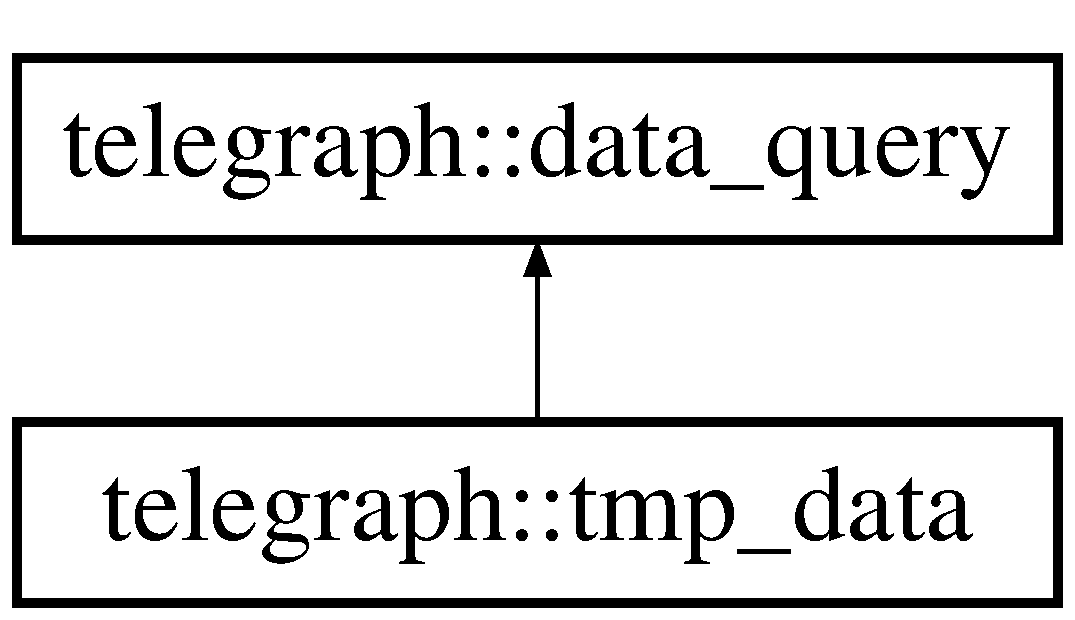
\includegraphics[height=2.000000cm]{classtelegraph_1_1data__query}
\end{center}
\end{figure}
\subsection*{Public Member Functions}
\begin{DoxyCompactItemize}
\item 
virtual const std\+::vector$<$ \hyperlink{classtelegraph_1_1data__point}{data\+\_\+point} $>$ \& \hyperlink{classtelegraph_1_1data__query_a20545e27166e025df2f73c13907bf721}{get\+\_\+current} () const =0
\end{DoxyCompactItemize}
\subsection*{Public Attributes}
\begin{DoxyCompactItemize}
\item 
\hyperlink{classtelegraph_1_1signal}{signal}$<$ const std\+::vector$<$ \hyperlink{classtelegraph_1_1data__point}{data\+\_\+point} $>$ \& $>$ \hyperlink{classtelegraph_1_1data__query_a81705835f67a1e5a4ce2c1009847eddc}{data}
\end{DoxyCompactItemize}


\subsection{Member Function Documentation}
\mbox{\Hypertarget{classtelegraph_1_1data__query_a20545e27166e025df2f73c13907bf721}\label{classtelegraph_1_1data__query_a20545e27166e025df2f73c13907bf721}} 
\index{telegraph\+::data\+\_\+query@{telegraph\+::data\+\_\+query}!get\+\_\+current@{get\+\_\+current}}
\index{get\+\_\+current@{get\+\_\+current}!telegraph\+::data\+\_\+query@{telegraph\+::data\+\_\+query}}
\subsubsection{\texorpdfstring{get\+\_\+current()}{get\_current()}}
{\footnotesize\ttfamily virtual const std\+::vector$<$\hyperlink{classtelegraph_1_1data__point}{data\+\_\+point}$>$\& telegraph\+::data\+\_\+query\+::get\+\_\+current (\begin{DoxyParamCaption}{ }\end{DoxyParamCaption}) const\hspace{0.3cm}{\ttfamily [pure virtual]}}



Implemented in \hyperlink{classtelegraph_1_1tmp__data_a0cc69096544afeaffaae5f25587dc62f}{telegraph\+::tmp\+\_\+data}.



\subsection{Member Data Documentation}
\mbox{\Hypertarget{classtelegraph_1_1data__query_a81705835f67a1e5a4ce2c1009847eddc}\label{classtelegraph_1_1data__query_a81705835f67a1e5a4ce2c1009847eddc}} 
\index{telegraph\+::data\+\_\+query@{telegraph\+::data\+\_\+query}!data@{data}}
\index{data@{data}!telegraph\+::data\+\_\+query@{telegraph\+::data\+\_\+query}}
\subsubsection{\texorpdfstring{data}{data}}
{\footnotesize\ttfamily \hyperlink{classtelegraph_1_1signal}{signal}$<$const std\+::vector$<$\hyperlink{classtelegraph_1_1data__point}{data\+\_\+point}$>$\&$>$ telegraph\+::data\+\_\+query\+::data}



The documentation for this class was generated from the following file\+:\begin{DoxyCompactItemize}
\item 
\hyperlink{data_8hpp}{data.\+hpp}\end{DoxyCompactItemize}

\hypertarget{classtelegraph_1_1device}{}\section{telegraph\+:\+:device Class Reference}
\label{classtelegraph_1_1device}\index{telegraph\+::device@{telegraph\+::device}}


{\ttfamily \#include $<$device.\+hpp$>$}

Inheritance diagram for telegraph\+:\+:device\+:\begin{figure}[H]
\begin{center}
\leavevmode
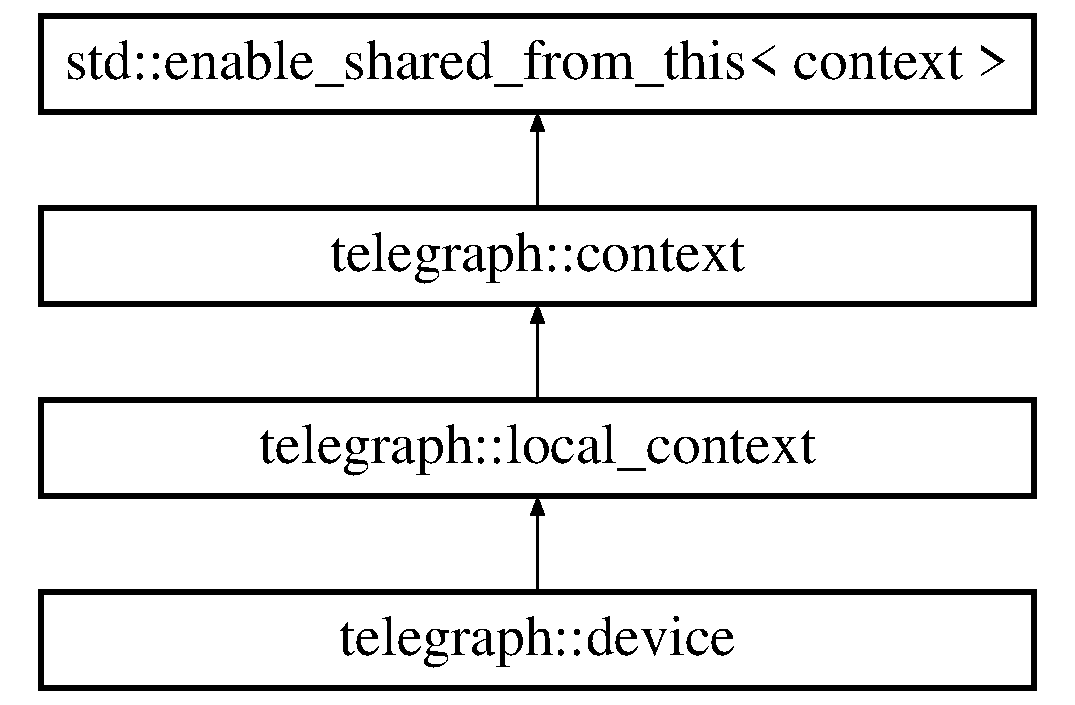
\includegraphics[height=4.000000cm]{classtelegraph_1_1device}
\end{center}
\end{figure}
\subsection*{Public Member Functions}
\begin{DoxyCompactItemize}
\item 
\hyperlink{classtelegraph_1_1device_a439a2eae3e8fceab20e87dea027dd912}{device} (io\+::io\+\_\+context \&ioc, const std\+::string \&name, const std\+::string \&port, int baud)
\item 
\hyperlink{classtelegraph_1_1device_a55d99b0a3df689b60480a54ebaab6a44}{$\sim$device} ()
\item 
void \hyperlink{classtelegraph_1_1device_a2f56da47b6e816ac9fd3b1ff2db5d2c9}{init} (\hyperlink{structboost_1_1asio_1_1yield__ctx}{io\+::yield\+\_\+ctx} \&, int millisec\+\_\+timeout)
\item 
\hyperlink{namespacetelegraph_ad071241508ea0f86c7de0686016f9ca9}{params\+\_\+stream\+\_\+ptr} \hyperlink{classtelegraph_1_1device_a9e5042e4640035b28dd9de780d7326df}{request} (\hyperlink{structboost_1_1asio_1_1yield__ctx}{io\+::yield\+\_\+ctx} \&, const \hyperlink{classtelegraph_1_1params}{params} \&p)
\item 
\hyperlink{namespacetelegraph_a58641aa5b1a2cbdb0431916a87069f64}{subscription\+\_\+ptr} \hyperlink{classtelegraph_1_1device_ab0117f6015f904afae72d6ab90c8ad95}{subscribe} (\hyperlink{structboost_1_1asio_1_1yield__ctx}{io\+::yield\+\_\+ctx} \&ctx, const \hyperlink{classtelegraph_1_1variable}{variable} $\ast$v, float min\+\_\+interval, float max\+\_\+interval, float timeout) override
\item 
\hyperlink{classtelegraph_1_1value}{value} \hyperlink{classtelegraph_1_1device_ac6558ddeed4799f4d69428863363a1e6}{call} (\hyperlink{structboost_1_1asio_1_1yield__ctx}{io\+::yield\+\_\+ctx} \&ctx, \hyperlink{classtelegraph_1_1action}{action} $\ast$a, \hyperlink{classtelegraph_1_1value}{value} v, float timeout)
\item 
void \hyperlink{classtelegraph_1_1device_a8d619b64e89b2ae933b282dc05956d37}{destroy} (\hyperlink{structboost_1_1asio_1_1yield__ctx}{io\+::yield\+\_\+ctx} \&ctx) override
\item 
\hyperlink{namespacetelegraph_a58641aa5b1a2cbdb0431916a87069f64}{subscription\+\_\+ptr} \hyperlink{classtelegraph_1_1device_aedf52d2dbb133e2b71958c116671b9df}{subscribe} (\hyperlink{structboost_1_1asio_1_1yield__ctx}{io\+::yield\+\_\+ctx} \&ctx, const std\+::vector$<$ std\+::string\+\_\+view $>$ \&path, float min\+\_\+interval, float max\+\_\+interval, float timeout) override
\item 
\hyperlink{classtelegraph_1_1value}{value} \hyperlink{classtelegraph_1_1device_a581368ab8f35ef72db17d2e330ded068}{call} (\hyperlink{structboost_1_1asio_1_1yield__ctx}{io\+::yield\+\_\+ctx} \&ctx, const std\+::vector$<$ std\+::string\+\_\+view $>$ \&path, \hyperlink{classtelegraph_1_1value}{value} v, float timeout) override
\item 
bool \hyperlink{classtelegraph_1_1device_a60150e55bc6fb63d27252051caf462db}{write\+\_\+data} (\hyperlink{structboost_1_1asio_1_1yield__ctx}{io\+::yield\+\_\+ctx} \&, \hyperlink{classtelegraph_1_1variable}{variable} $\ast$v, const std\+::vector$<$ \hyperlink{classtelegraph_1_1data__point}{data\+\_\+point} $>$ \&d) override
\item 
bool \hyperlink{classtelegraph_1_1device_aaedca7b20bc36f8439d5afccbcaf1304}{write\+\_\+data} (\hyperlink{structboost_1_1asio_1_1yield__ctx}{io\+::yield\+\_\+ctx} \&, const std\+::vector$<$ std\+::string\+\_\+view $>$ \&path, const std\+::vector$<$ \hyperlink{classtelegraph_1_1data__point}{data\+\_\+point} $>$ \&d) override
\item 
\hyperlink{namespacetelegraph_a6ffe775ac48dca2a4013b53d692199c8}{data\+\_\+query\+\_\+ptr} \hyperlink{classtelegraph_1_1device_a4c46c7e98bf5a573a9966fd2cc199021}{query\+\_\+data} (\hyperlink{structboost_1_1asio_1_1yield__ctx}{io\+::yield\+\_\+ctx} \&yield, const \hyperlink{classtelegraph_1_1variable}{variable} $\ast$n) override
\item 
\hyperlink{namespacetelegraph_a6ffe775ac48dca2a4013b53d692199c8}{data\+\_\+query\+\_\+ptr} \hyperlink{classtelegraph_1_1device_a9a5ef799aadf591a355cc1e50442d762}{query\+\_\+data} (\hyperlink{structboost_1_1asio_1_1yield__ctx}{io\+::yield\+\_\+ctx} \&yield, const std\+::vector$<$ std\+::string\+\_\+view $>$ \&p) override
\end{DoxyCompactItemize}
\subsection*{Static Public Member Functions}
\begin{DoxyCompactItemize}
\item 
static \hyperlink{namespacetelegraph_ab59c7b38d99a98b4acc22433c920b1e6}{local\+\_\+context\+\_\+ptr} \hyperlink{classtelegraph_1_1device_a4bb333fc0232bdb69283e71f086028c4}{create} (\hyperlink{structboost_1_1asio_1_1yield__ctx}{io\+::yield\+\_\+ctx} \&, io\+::io\+\_\+context \&ioc, const std\+::string\+\_\+view \&name, const std\+::string\+\_\+view \&type, const \hyperlink{classtelegraph_1_1params}{params} \&p)
\end{DoxyCompactItemize}
\subsection*{Additional Inherited Members}


\subsection{Constructor \& Destructor Documentation}
\mbox{\Hypertarget{classtelegraph_1_1device_a439a2eae3e8fceab20e87dea027dd912}\label{classtelegraph_1_1device_a439a2eae3e8fceab20e87dea027dd912}} 
\index{telegraph\+::device@{telegraph\+::device}!device@{device}}
\index{device@{device}!telegraph\+::device@{telegraph\+::device}}
\subsubsection{\texorpdfstring{device()}{device()}}
{\footnotesize\ttfamily telegraph\+::device\+::device (\begin{DoxyParamCaption}\item[{io\+::io\+\_\+context \&}]{ioc,  }\item[{const std\+::string \&}]{name,  }\item[{const std\+::string \&}]{port,  }\item[{int}]{baud }\end{DoxyParamCaption})}

\mbox{\Hypertarget{classtelegraph_1_1device_a55d99b0a3df689b60480a54ebaab6a44}\label{classtelegraph_1_1device_a55d99b0a3df689b60480a54ebaab6a44}} 
\index{telegraph\+::device@{telegraph\+::device}!````~device@{$\sim$device}}
\index{````~device@{$\sim$device}!telegraph\+::device@{telegraph\+::device}}
\subsubsection{\texorpdfstring{$\sim$device()}{~device()}}
{\footnotesize\ttfamily telegraph\+::device\+::$\sim$device (\begin{DoxyParamCaption}{ }\end{DoxyParamCaption})}



\subsection{Member Function Documentation}
\mbox{\Hypertarget{classtelegraph_1_1device_ac6558ddeed4799f4d69428863363a1e6}\label{classtelegraph_1_1device_ac6558ddeed4799f4d69428863363a1e6}} 
\index{telegraph\+::device@{telegraph\+::device}!call@{call}}
\index{call@{call}!telegraph\+::device@{telegraph\+::device}}
\subsubsection{\texorpdfstring{call()}{call()}\hspace{0.1cm}{\footnotesize\ttfamily [1/2]}}
{\footnotesize\ttfamily \hyperlink{classtelegraph_1_1value}{value} telegraph\+::device\+::call (\begin{DoxyParamCaption}\item[{\hyperlink{structboost_1_1asio_1_1yield__ctx}{io\+::yield\+\_\+ctx} \&}]{ctx,  }\item[{\hyperlink{classtelegraph_1_1action}{action} $\ast$}]{a,  }\item[{\hyperlink{classtelegraph_1_1value}{value}}]{v,  }\item[{float}]{timeout }\end{DoxyParamCaption})\hspace{0.3cm}{\ttfamily [virtual]}}



Implements \hyperlink{classtelegraph_1_1context_a72da471eb635e5505b10d2f1103359ac}{telegraph\+::context}.

\mbox{\Hypertarget{classtelegraph_1_1device_a581368ab8f35ef72db17d2e330ded068}\label{classtelegraph_1_1device_a581368ab8f35ef72db17d2e330ded068}} 
\index{telegraph\+::device@{telegraph\+::device}!call@{call}}
\index{call@{call}!telegraph\+::device@{telegraph\+::device}}
\subsubsection{\texorpdfstring{call()}{call()}\hspace{0.1cm}{\footnotesize\ttfamily [2/2]}}
{\footnotesize\ttfamily \hyperlink{classtelegraph_1_1value}{value} telegraph\+::device\+::call (\begin{DoxyParamCaption}\item[{\hyperlink{structboost_1_1asio_1_1yield__ctx}{io\+::yield\+\_\+ctx} \&}]{ctx,  }\item[{const std\+::vector$<$ std\+::string\+\_\+view $>$ \&}]{path,  }\item[{\hyperlink{classtelegraph_1_1value}{value}}]{v,  }\item[{float}]{timeout }\end{DoxyParamCaption})\hspace{0.3cm}{\ttfamily [inline]}, {\ttfamily [override]}, {\ttfamily [virtual]}}



Implements \hyperlink{classtelegraph_1_1context_a0798d49ea0874a870d4c980f6f09b6c2}{telegraph\+::context}.

\mbox{\Hypertarget{classtelegraph_1_1device_a4bb333fc0232bdb69283e71f086028c4}\label{classtelegraph_1_1device_a4bb333fc0232bdb69283e71f086028c4}} 
\index{telegraph\+::device@{telegraph\+::device}!create@{create}}
\index{create@{create}!telegraph\+::device@{telegraph\+::device}}
\subsubsection{\texorpdfstring{create()}{create()}}
{\footnotesize\ttfamily \hyperlink{namespacetelegraph_ab59c7b38d99a98b4acc22433c920b1e6}{local\+\_\+context\+\_\+ptr} telegraph\+::device\+::create (\begin{DoxyParamCaption}\item[{\hyperlink{structboost_1_1asio_1_1yield__ctx}{io\+::yield\+\_\+ctx} \&}]{yield,  }\item[{io\+::io\+\_\+context \&}]{ioc,  }\item[{const std\+::string\+\_\+view \&}]{name,  }\item[{const std\+::string\+\_\+view \&}]{type,  }\item[{const \hyperlink{classtelegraph_1_1params}{params} \&}]{p }\end{DoxyParamCaption})\hspace{0.3cm}{\ttfamily [static]}}

\mbox{\Hypertarget{classtelegraph_1_1device_a8d619b64e89b2ae933b282dc05956d37}\label{classtelegraph_1_1device_a8d619b64e89b2ae933b282dc05956d37}} 
\index{telegraph\+::device@{telegraph\+::device}!destroy@{destroy}}
\index{destroy@{destroy}!telegraph\+::device@{telegraph\+::device}}
\subsubsection{\texorpdfstring{destroy()}{destroy()}}
{\footnotesize\ttfamily void telegraph\+::device\+::destroy (\begin{DoxyParamCaption}\item[{\hyperlink{structboost_1_1asio_1_1yield__ctx}{io\+::yield\+\_\+ctx} \&}]{ctx }\end{DoxyParamCaption})\hspace{0.3cm}{\ttfamily [override]}, {\ttfamily [virtual]}}



Implements \hyperlink{classtelegraph_1_1context_a4017c1bcd9c84170a5cb612ae45d6fb4}{telegraph\+::context}.

\mbox{\Hypertarget{classtelegraph_1_1device_a2f56da47b6e816ac9fd3b1ff2db5d2c9}\label{classtelegraph_1_1device_a2f56da47b6e816ac9fd3b1ff2db5d2c9}} 
\index{telegraph\+::device@{telegraph\+::device}!init@{init}}
\index{init@{init}!telegraph\+::device@{telegraph\+::device}}
\subsubsection{\texorpdfstring{init()}{init()}}
{\footnotesize\ttfamily void telegraph\+::device\+::init (\begin{DoxyParamCaption}\item[{\hyperlink{structboost_1_1asio_1_1yield__ctx}{io\+::yield\+\_\+ctx} \&}]{yield,  }\item[{int}]{millisec\+\_\+timeout }\end{DoxyParamCaption})}

\mbox{\Hypertarget{classtelegraph_1_1device_a4c46c7e98bf5a573a9966fd2cc199021}\label{classtelegraph_1_1device_a4c46c7e98bf5a573a9966fd2cc199021}} 
\index{telegraph\+::device@{telegraph\+::device}!query\+\_\+data@{query\+\_\+data}}
\index{query\+\_\+data@{query\+\_\+data}!telegraph\+::device@{telegraph\+::device}}
\subsubsection{\texorpdfstring{query\+\_\+data()}{query\_data()}\hspace{0.1cm}{\footnotesize\ttfamily [1/2]}}
{\footnotesize\ttfamily \hyperlink{namespacetelegraph_a6ffe775ac48dca2a4013b53d692199c8}{data\+\_\+query\+\_\+ptr} telegraph\+::device\+::query\+\_\+data (\begin{DoxyParamCaption}\item[{\hyperlink{structboost_1_1asio_1_1yield__ctx}{io\+::yield\+\_\+ctx} \&}]{yield,  }\item[{const \hyperlink{classtelegraph_1_1variable}{variable} $\ast$}]{n }\end{DoxyParamCaption})\hspace{0.3cm}{\ttfamily [inline]}, {\ttfamily [override]}, {\ttfamily [virtual]}}



Implements \hyperlink{classtelegraph_1_1context_a301114c9b73194507ae58221566a3e57}{telegraph\+::context}.

\mbox{\Hypertarget{classtelegraph_1_1device_a9a5ef799aadf591a355cc1e50442d762}\label{classtelegraph_1_1device_a9a5ef799aadf591a355cc1e50442d762}} 
\index{telegraph\+::device@{telegraph\+::device}!query\+\_\+data@{query\+\_\+data}}
\index{query\+\_\+data@{query\+\_\+data}!telegraph\+::device@{telegraph\+::device}}
\subsubsection{\texorpdfstring{query\+\_\+data()}{query\_data()}\hspace{0.1cm}{\footnotesize\ttfamily [2/2]}}
{\footnotesize\ttfamily \hyperlink{namespacetelegraph_a6ffe775ac48dca2a4013b53d692199c8}{data\+\_\+query\+\_\+ptr} telegraph\+::device\+::query\+\_\+data (\begin{DoxyParamCaption}\item[{\hyperlink{structboost_1_1asio_1_1yield__ctx}{io\+::yield\+\_\+ctx} \&}]{yield,  }\item[{const std\+::vector$<$ std\+::string\+\_\+view $>$ \&}]{p }\end{DoxyParamCaption})\hspace{0.3cm}{\ttfamily [inline]}, {\ttfamily [override]}, {\ttfamily [virtual]}}



Implements \hyperlink{classtelegraph_1_1context_a34793623d2a2def580ad0b8710c74c6d}{telegraph\+::context}.

\mbox{\Hypertarget{classtelegraph_1_1device_a9e5042e4640035b28dd9de780d7326df}\label{classtelegraph_1_1device_a9e5042e4640035b28dd9de780d7326df}} 
\index{telegraph\+::device@{telegraph\+::device}!request@{request}}
\index{request@{request}!telegraph\+::device@{telegraph\+::device}}
\subsubsection{\texorpdfstring{request()}{request()}}
{\footnotesize\ttfamily \hyperlink{namespacetelegraph_ad071241508ea0f86c7de0686016f9ca9}{params\+\_\+stream\+\_\+ptr} telegraph\+::device\+::request (\begin{DoxyParamCaption}\item[{\hyperlink{structboost_1_1asio_1_1yield__ctx}{io\+::yield\+\_\+ctx} \&}]{,  }\item[{const \hyperlink{classtelegraph_1_1params}{params} \&}]{p }\end{DoxyParamCaption})\hspace{0.3cm}{\ttfamily [inline]}, {\ttfamily [virtual]}}



Implements \hyperlink{classtelegraph_1_1context_a6765d7fa22fe99b9a6723c511396b781}{telegraph\+::context}.

\mbox{\Hypertarget{classtelegraph_1_1device_ab0117f6015f904afae72d6ab90c8ad95}\label{classtelegraph_1_1device_ab0117f6015f904afae72d6ab90c8ad95}} 
\index{telegraph\+::device@{telegraph\+::device}!subscribe@{subscribe}}
\index{subscribe@{subscribe}!telegraph\+::device@{telegraph\+::device}}
\subsubsection{\texorpdfstring{subscribe()}{subscribe()}\hspace{0.1cm}{\footnotesize\ttfamily [1/2]}}
{\footnotesize\ttfamily \hyperlink{namespacetelegraph_a58641aa5b1a2cbdb0431916a87069f64}{subscription\+\_\+ptr} telegraph\+::device\+::subscribe (\begin{DoxyParamCaption}\item[{\hyperlink{structboost_1_1asio_1_1yield__ctx}{io\+::yield\+\_\+ctx} \&}]{ctx,  }\item[{const \hyperlink{classtelegraph_1_1variable}{variable} $\ast$}]{v,  }\item[{float}]{min\+\_\+interval,  }\item[{float}]{max\+\_\+interval,  }\item[{float}]{timeout }\end{DoxyParamCaption})\hspace{0.3cm}{\ttfamily [override]}, {\ttfamily [virtual]}}



Implements \hyperlink{classtelegraph_1_1context_aec3b3b0d7210a86f2ea2f5067ef8e922}{telegraph\+::context}.

\mbox{\Hypertarget{classtelegraph_1_1device_aedf52d2dbb133e2b71958c116671b9df}\label{classtelegraph_1_1device_aedf52d2dbb133e2b71958c116671b9df}} 
\index{telegraph\+::device@{telegraph\+::device}!subscribe@{subscribe}}
\index{subscribe@{subscribe}!telegraph\+::device@{telegraph\+::device}}
\subsubsection{\texorpdfstring{subscribe()}{subscribe()}\hspace{0.1cm}{\footnotesize\ttfamily [2/2]}}
{\footnotesize\ttfamily \hyperlink{namespacetelegraph_a58641aa5b1a2cbdb0431916a87069f64}{subscription\+\_\+ptr} telegraph\+::device\+::subscribe (\begin{DoxyParamCaption}\item[{\hyperlink{structboost_1_1asio_1_1yield__ctx}{io\+::yield\+\_\+ctx} \&}]{ctx,  }\item[{const std\+::vector$<$ std\+::string\+\_\+view $>$ \&}]{path,  }\item[{float}]{min\+\_\+interval,  }\item[{float}]{max\+\_\+interval,  }\item[{float}]{timeout }\end{DoxyParamCaption})\hspace{0.3cm}{\ttfamily [inline]}, {\ttfamily [override]}, {\ttfamily [virtual]}}



Implements \hyperlink{classtelegraph_1_1context_a8db167973f187f707a4108e112683969}{telegraph\+::context}.

\mbox{\Hypertarget{classtelegraph_1_1device_a60150e55bc6fb63d27252051caf462db}\label{classtelegraph_1_1device_a60150e55bc6fb63d27252051caf462db}} 
\index{telegraph\+::device@{telegraph\+::device}!write\+\_\+data@{write\+\_\+data}}
\index{write\+\_\+data@{write\+\_\+data}!telegraph\+::device@{telegraph\+::device}}
\subsubsection{\texorpdfstring{write\+\_\+data()}{write\_data()}\hspace{0.1cm}{\footnotesize\ttfamily [1/2]}}
{\footnotesize\ttfamily bool telegraph\+::device\+::write\+\_\+data (\begin{DoxyParamCaption}\item[{\hyperlink{structboost_1_1asio_1_1yield__ctx}{io\+::yield\+\_\+ctx} \&}]{,  }\item[{\hyperlink{classtelegraph_1_1variable}{variable} $\ast$}]{v,  }\item[{const std\+::vector$<$ \hyperlink{classtelegraph_1_1data__point}{data\+\_\+point} $>$ \&}]{d }\end{DoxyParamCaption})\hspace{0.3cm}{\ttfamily [inline]}, {\ttfamily [override]}, {\ttfamily [virtual]}}



Implements \hyperlink{classtelegraph_1_1context_a6067b9a6f2590733c81f6a3b2ed9cba7}{telegraph\+::context}.

\mbox{\Hypertarget{classtelegraph_1_1device_aaedca7b20bc36f8439d5afccbcaf1304}\label{classtelegraph_1_1device_aaedca7b20bc36f8439d5afccbcaf1304}} 
\index{telegraph\+::device@{telegraph\+::device}!write\+\_\+data@{write\+\_\+data}}
\index{write\+\_\+data@{write\+\_\+data}!telegraph\+::device@{telegraph\+::device}}
\subsubsection{\texorpdfstring{write\+\_\+data()}{write\_data()}\hspace{0.1cm}{\footnotesize\ttfamily [2/2]}}
{\footnotesize\ttfamily bool telegraph\+::device\+::write\+\_\+data (\begin{DoxyParamCaption}\item[{\hyperlink{structboost_1_1asio_1_1yield__ctx}{io\+::yield\+\_\+ctx} \&}]{,  }\item[{const std\+::vector$<$ std\+::string\+\_\+view $>$ \&}]{path,  }\item[{const std\+::vector$<$ \hyperlink{classtelegraph_1_1data__point}{data\+\_\+point} $>$ \&}]{d }\end{DoxyParamCaption})\hspace{0.3cm}{\ttfamily [inline]}, {\ttfamily [override]}, {\ttfamily [virtual]}}



Implements \hyperlink{classtelegraph_1_1context_a1f600d6159df21dd2750b1c706ca3412}{telegraph\+::context}.



The documentation for this class was generated from the following files\+:\begin{DoxyCompactItemize}
\item 
\hyperlink{device_8hpp}{device.\+hpp}\item 
\hyperlink{device_8cpp}{device.\+cpp}\end{DoxyCompactItemize}

\hypertarget{classtelegraph_1_1device__scanner}{}\section{telegraph\+:\+:device\+\_\+scanner Class Reference}
\label{classtelegraph_1_1device__scanner}\index{telegraph\+::device\+\_\+scanner@{telegraph\+::device\+\_\+scanner}}


{\ttfamily \#include $<$device.\+hpp$>$}

Inheritance diagram for telegraph\+:\+:device\+\_\+scanner\+:\begin{figure}[H]
\begin{center}
\leavevmode
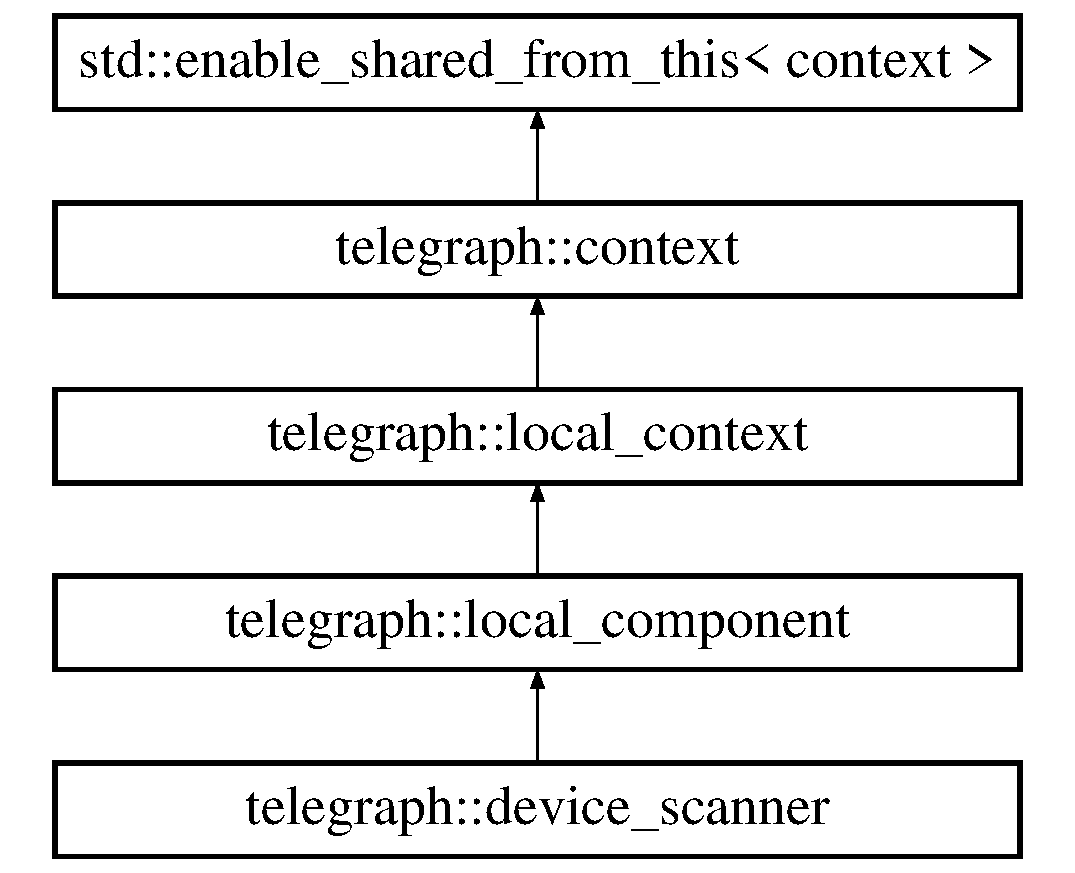
\includegraphics[height=5.000000cm]{classtelegraph_1_1device__scanner}
\end{center}
\end{figure}
\subsection*{Public Member Functions}
\begin{DoxyCompactItemize}
\item 
\hyperlink{classtelegraph_1_1device__scanner_a6e8057b68307b61500ed615248dcd730}{device\+\_\+scanner} (io\+::io\+\_\+context \&ioc, const std\+::string\+\_\+view \&name)
\item 
\hyperlink{classtelegraph_1_1device__scanner_a3d900bd95a620d086954562c669f91d9}{$\sim$device\+\_\+scanner} ()
\item 
void \hyperlink{classtelegraph_1_1device__scanner_a71be73d87ccb72b5311ad19aab16c1c7}{init} ()
\item 
\hyperlink{namespacetelegraph_ad071241508ea0f86c7de0686016f9ca9}{params\+\_\+stream\+\_\+ptr} \hyperlink{classtelegraph_1_1device__scanner_a5873278cb04e50896c3f125639df4c73}{request} (\hyperlink{structboost_1_1asio_1_1yield__ctx}{io\+::yield\+\_\+ctx} \&, const \hyperlink{classtelegraph_1_1params}{params} \&p) override
\end{DoxyCompactItemize}
\subsection*{Static Public Member Functions}
\begin{DoxyCompactItemize}
\item 
static \hyperlink{namespacetelegraph_a69cfb42be07c9189123cfa3ff3ec4487}{local\+\_\+component\+\_\+ptr} \hyperlink{classtelegraph_1_1device__scanner_a53b359ed0ed7088cdaf4d78658936a8d}{create} (\hyperlink{structboost_1_1asio_1_1yield__ctx}{io\+::yield\+\_\+ctx} \&, io\+::io\+\_\+context \&ioc, const std\+::string\+\_\+view \&name, const std\+::string\+\_\+view \&type, const \hyperlink{classtelegraph_1_1params}{params} \&p)
\end{DoxyCompactItemize}
\subsection*{Additional Inherited Members}


\subsection{Constructor \& Destructor Documentation}
\mbox{\Hypertarget{classtelegraph_1_1device__scanner_a6e8057b68307b61500ed615248dcd730}\label{classtelegraph_1_1device__scanner_a6e8057b68307b61500ed615248dcd730}} 
\index{telegraph\+::device\+\_\+scanner@{telegraph\+::device\+\_\+scanner}!device\+\_\+scanner@{device\+\_\+scanner}}
\index{device\+\_\+scanner@{device\+\_\+scanner}!telegraph\+::device\+\_\+scanner@{telegraph\+::device\+\_\+scanner}}
\subsubsection{\texorpdfstring{device\+\_\+scanner()}{device\_scanner()}}
{\footnotesize\ttfamily telegraph\+::device\+\_\+scanner\+::device\+\_\+scanner (\begin{DoxyParamCaption}\item[{io\+::io\+\_\+context \&}]{ioc,  }\item[{const std\+::string\+\_\+view \&}]{name }\end{DoxyParamCaption})}

\mbox{\Hypertarget{classtelegraph_1_1device__scanner_a3d900bd95a620d086954562c669f91d9}\label{classtelegraph_1_1device__scanner_a3d900bd95a620d086954562c669f91d9}} 
\index{telegraph\+::device\+\_\+scanner@{telegraph\+::device\+\_\+scanner}!````~device\+\_\+scanner@{$\sim$device\+\_\+scanner}}
\index{````~device\+\_\+scanner@{$\sim$device\+\_\+scanner}!telegraph\+::device\+\_\+scanner@{telegraph\+::device\+\_\+scanner}}
\subsubsection{\texorpdfstring{$\sim$device\+\_\+scanner()}{~device\_scanner()}}
{\footnotesize\ttfamily telegraph\+::device\+\_\+scanner\+::$\sim$device\+\_\+scanner (\begin{DoxyParamCaption}{ }\end{DoxyParamCaption})}



\subsection{Member Function Documentation}
\mbox{\Hypertarget{classtelegraph_1_1device__scanner_a53b359ed0ed7088cdaf4d78658936a8d}\label{classtelegraph_1_1device__scanner_a53b359ed0ed7088cdaf4d78658936a8d}} 
\index{telegraph\+::device\+\_\+scanner@{telegraph\+::device\+\_\+scanner}!create@{create}}
\index{create@{create}!telegraph\+::device\+\_\+scanner@{telegraph\+::device\+\_\+scanner}}
\subsubsection{\texorpdfstring{create()}{create()}}
{\footnotesize\ttfamily \hyperlink{namespacetelegraph_a69cfb42be07c9189123cfa3ff3ec4487}{local\+\_\+component\+\_\+ptr} telegraph\+::device\+\_\+scanner\+::create (\begin{DoxyParamCaption}\item[{\hyperlink{structboost_1_1asio_1_1yield__ctx}{io\+::yield\+\_\+ctx} \&}]{,  }\item[{io\+::io\+\_\+context \&}]{ioc,  }\item[{const std\+::string\+\_\+view \&}]{name,  }\item[{const std\+::string\+\_\+view \&}]{type,  }\item[{const \hyperlink{classtelegraph_1_1params}{params} \&}]{p }\end{DoxyParamCaption})\hspace{0.3cm}{\ttfamily [static]}}

\mbox{\Hypertarget{classtelegraph_1_1device__scanner_a71be73d87ccb72b5311ad19aab16c1c7}\label{classtelegraph_1_1device__scanner_a71be73d87ccb72b5311ad19aab16c1c7}} 
\index{telegraph\+::device\+\_\+scanner@{telegraph\+::device\+\_\+scanner}!init@{init}}
\index{init@{init}!telegraph\+::device\+\_\+scanner@{telegraph\+::device\+\_\+scanner}}
\subsubsection{\texorpdfstring{init()}{init()}}
{\footnotesize\ttfamily void telegraph\+::device\+\_\+scanner\+::init (\begin{DoxyParamCaption}{ }\end{DoxyParamCaption})}

\mbox{\Hypertarget{classtelegraph_1_1device__scanner_a5873278cb04e50896c3f125639df4c73}\label{classtelegraph_1_1device__scanner_a5873278cb04e50896c3f125639df4c73}} 
\index{telegraph\+::device\+\_\+scanner@{telegraph\+::device\+\_\+scanner}!request@{request}}
\index{request@{request}!telegraph\+::device\+\_\+scanner@{telegraph\+::device\+\_\+scanner}}
\subsubsection{\texorpdfstring{request()}{request()}}
{\footnotesize\ttfamily \hyperlink{namespacetelegraph_ad071241508ea0f86c7de0686016f9ca9}{params\+\_\+stream\+\_\+ptr} telegraph\+::device\+\_\+scanner\+::request (\begin{DoxyParamCaption}\item[{\hyperlink{structboost_1_1asio_1_1yield__ctx}{io\+::yield\+\_\+ctx} \&}]{yield,  }\item[{const \hyperlink{classtelegraph_1_1params}{params} \&}]{p }\end{DoxyParamCaption})\hspace{0.3cm}{\ttfamily [override]}, {\ttfamily [virtual]}}



Implements \hyperlink{classtelegraph_1_1context_a6765d7fa22fe99b9a6723c511396b781}{telegraph\+::context}.



The documentation for this class was generated from the following files\+:\begin{DoxyCompactItemize}
\item 
\hyperlink{device_8hpp}{device.\+hpp}\item 
\hyperlink{device_8cpp}{device.\+cpp}\end{DoxyCompactItemize}

\hypertarget{structstdext_1_1inplace__function__detail_1_1aligned__storage__helper_1_1double1}{}\section{stdext\+:\+:inplace\+\_\+function\+\_\+detail\+:\+:aligned\+\_\+storage\+\_\+helper$<$ Cap $>$\+:\+:double1 Struct Reference}
\label{structstdext_1_1inplace__function__detail_1_1aligned__storage__helper_1_1double1}\index{stdext\+::inplace\+\_\+function\+\_\+detail\+::aligned\+\_\+storage\+\_\+helper$<$ Cap $>$\+::double1@{stdext\+::inplace\+\_\+function\+\_\+detail\+::aligned\+\_\+storage\+\_\+helper$<$ Cap $>$\+::double1}}


{\ttfamily \#include $<$inplace\+\_\+function.\+hpp$>$}

\subsection*{Public Attributes}
\begin{DoxyCompactItemize}
\item 
double \hyperlink{structstdext_1_1inplace__function__detail_1_1aligned__storage__helper_1_1double1_a21bd2ba02bde2bd642aff6bdee37407f}{a}
\end{DoxyCompactItemize}


\subsection{Member Data Documentation}
\mbox{\Hypertarget{structstdext_1_1inplace__function__detail_1_1aligned__storage__helper_1_1double1_a21bd2ba02bde2bd642aff6bdee37407f}\label{structstdext_1_1inplace__function__detail_1_1aligned__storage__helper_1_1double1_a21bd2ba02bde2bd642aff6bdee37407f}} 
\index{stdext\+::inplace\+\_\+function\+\_\+detail\+::aligned\+\_\+storage\+\_\+helper\+::double1@{stdext\+::inplace\+\_\+function\+\_\+detail\+::aligned\+\_\+storage\+\_\+helper\+::double1}!a@{a}}
\index{a@{a}!stdext\+::inplace\+\_\+function\+\_\+detail\+::aligned\+\_\+storage\+\_\+helper\+::double1@{stdext\+::inplace\+\_\+function\+\_\+detail\+::aligned\+\_\+storage\+\_\+helper\+::double1}}
\subsubsection{\texorpdfstring{a}{a}}
{\footnotesize\ttfamily template$<$size\+\_\+t Cap$>$ \\
double \hyperlink{unionstdext_1_1inplace__function__detail_1_1aligned__storage__helper}{stdext\+::inplace\+\_\+function\+\_\+detail\+::aligned\+\_\+storage\+\_\+helper}$<$ Cap $>$\+::double1\+::a}



The documentation for this struct was generated from the following file\+:\begin{DoxyCompactItemize}
\item 
\hyperlink{gen_2telegen_2inplace__function_8hpp}{gen/telegen/inplace\+\_\+function.\+hpp}\end{DoxyCompactItemize}

\hypertarget{structstdext_1_1inplace__function__detail_1_1aligned__storage__helper_1_1double4}{}\section{stdext\+:\+:inplace\+\_\+function\+\_\+detail\+:\+:aligned\+\_\+storage\+\_\+helper$<$ Cap $>$\+:\+:double4 Struct Reference}
\label{structstdext_1_1inplace__function__detail_1_1aligned__storage__helper_1_1double4}\index{stdext\+::inplace\+\_\+function\+\_\+detail\+::aligned\+\_\+storage\+\_\+helper$<$ Cap $>$\+::double4@{stdext\+::inplace\+\_\+function\+\_\+detail\+::aligned\+\_\+storage\+\_\+helper$<$ Cap $>$\+::double4}}


{\ttfamily \#include $<$inplace\+\_\+function.\+hpp$>$}

\subsection*{Public Attributes}
\begin{DoxyCompactItemize}
\item 
double \hyperlink{structstdext_1_1inplace__function__detail_1_1aligned__storage__helper_1_1double4_a02373c793fa67c6b57d24d2f34b58504}{a} \mbox{[}4\mbox{]}
\end{DoxyCompactItemize}


\subsection{Member Data Documentation}
\mbox{\Hypertarget{structstdext_1_1inplace__function__detail_1_1aligned__storage__helper_1_1double4_a02373c793fa67c6b57d24d2f34b58504}\label{structstdext_1_1inplace__function__detail_1_1aligned__storage__helper_1_1double4_a02373c793fa67c6b57d24d2f34b58504}} 
\index{stdext\+::inplace\+\_\+function\+\_\+detail\+::aligned\+\_\+storage\+\_\+helper\+::double4@{stdext\+::inplace\+\_\+function\+\_\+detail\+::aligned\+\_\+storage\+\_\+helper\+::double4}!a@{a}}
\index{a@{a}!stdext\+::inplace\+\_\+function\+\_\+detail\+::aligned\+\_\+storage\+\_\+helper\+::double4@{stdext\+::inplace\+\_\+function\+\_\+detail\+::aligned\+\_\+storage\+\_\+helper\+::double4}}
\subsubsection{\texorpdfstring{a}{a}}
{\footnotesize\ttfamily template$<$size\+\_\+t Cap$>$ \\
double \hyperlink{unionstdext_1_1inplace__function__detail_1_1aligned__storage__helper}{stdext\+::inplace\+\_\+function\+\_\+detail\+::aligned\+\_\+storage\+\_\+helper}$<$ Cap $>$\+::double4\+::a}



The documentation for this struct was generated from the following file\+:\begin{DoxyCompactItemize}
\item 
\hyperlink{gen_2telegen_2inplace__function_8hpp}{gen/telegen/inplace\+\_\+function.\+hpp}\end{DoxyCompactItemize}

\hypertarget{classtelegraph_1_1dummy__device}{}\section{telegraph\+:\+:dummy\+\_\+device Class Reference}
\label{classtelegraph_1_1dummy__device}\index{telegraph\+::dummy\+\_\+device@{telegraph\+::dummy\+\_\+device}}


{\ttfamily \#include $<$dummy\+\_\+device.\+hpp$>$}

Inheritance diagram for telegraph\+:\+:dummy\+\_\+device\+:\begin{figure}[H]
\begin{center}
\leavevmode
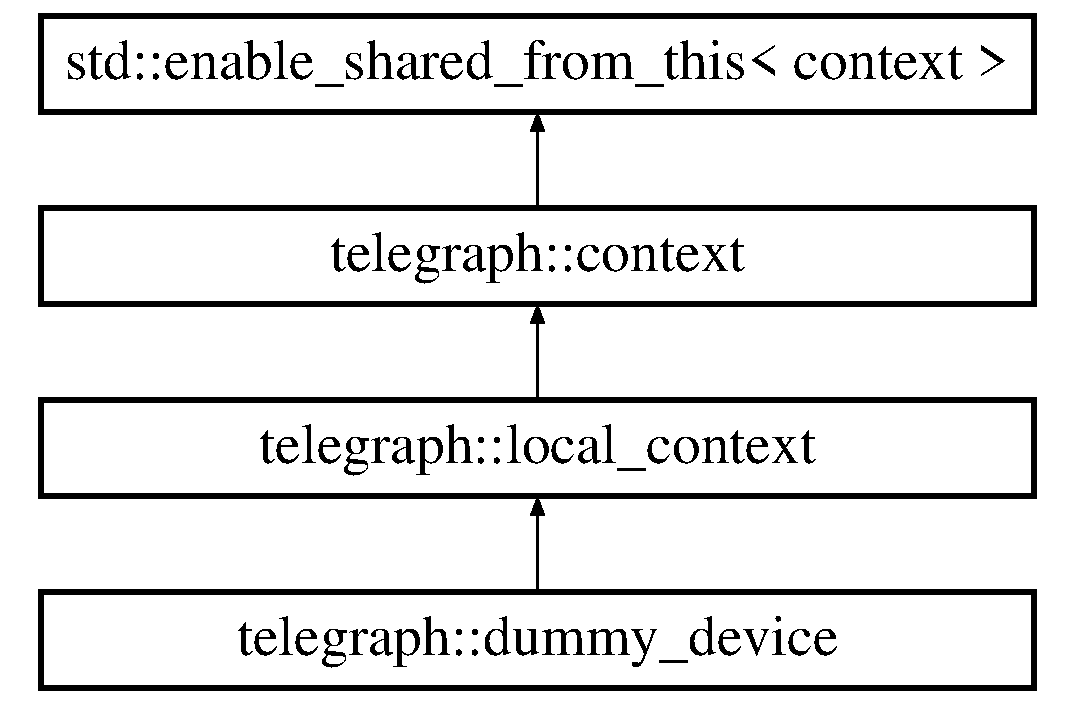
\includegraphics[height=4.000000cm]{classtelegraph_1_1dummy__device}
\end{center}
\end{figure}
\subsection*{Public Types}
\begin{DoxyCompactItemize}
\item 
using \hyperlink{classtelegraph_1_1dummy__device_a608031386eb0abf2fc578211c1270f89}{handler} = std\+::function$<$ void(\hyperlink{structboost_1_1asio_1_1yield__ctx}{io\+::yield\+\_\+ctx} \&, \hyperlink{classtelegraph_1_1value}{value})$>$
\end{DoxyCompactItemize}
\subsection*{Public Member Functions}
\begin{DoxyCompactItemize}
\item 
\hyperlink{classtelegraph_1_1dummy__device_a70f00acd6141dea4c68f3b1f51c06cf0}{dummy\+\_\+device} (io\+::io\+\_\+context \&ioc, const std\+::string\+\_\+view \&name, std\+::unique\+\_\+ptr$<$ \hyperlink{classtelegraph_1_1node}{node} $>$ \&\&s)
\item 
\hyperlink{classtelegraph_1_1dummy__device_a7c2ea565d75451d04eaaba128be2550a}{$\sim$dummy\+\_\+device} ()
\item 
void \hyperlink{classtelegraph_1_1dummy__device_a577a558745fcfddca641a80390ced80d}{add\+\_\+publisher} (const \hyperlink{classtelegraph_1_1variable}{variable} $\ast$v, const \hyperlink{namespacetelegraph_aff5109352406dd9a8cd38f431f808bc5}{publisher\+\_\+ptr} \&p)
\item 
void \hyperlink{classtelegraph_1_1dummy__device_abf7bb4171f3bc0af89101f12a885d614}{add\+\_\+handler} (const \hyperlink{classtelegraph_1_1action}{action} $\ast$a, const \hyperlink{classtelegraph_1_1dummy__device_a608031386eb0abf2fc578211c1270f89}{handler} \&h)
\item 
\hyperlink{namespacetelegraph_ad071241508ea0f86c7de0686016f9ca9}{params\+\_\+stream\+\_\+ptr} \hyperlink{classtelegraph_1_1dummy__device_a46d728506b36e9e8b5b6939eb6aefe12}{request} (\hyperlink{structboost_1_1asio_1_1yield__ctx}{io\+::yield\+\_\+ctx} \&, const \hyperlink{classtelegraph_1_1params}{params} \&p) override
\item 
\hyperlink{namespacetelegraph_a58641aa5b1a2cbdb0431916a87069f64}{subscription\+\_\+ptr} \hyperlink{classtelegraph_1_1dummy__device_a06470ed069c481e8199dce9387448c8b}{subscribe} (\hyperlink{structboost_1_1asio_1_1yield__ctx}{io\+::yield\+\_\+ctx} \&ctx, const \hyperlink{classtelegraph_1_1variable}{variable} $\ast$v, float min\+\_\+interval, float max\+\_\+interval, float timeout) override
\item 
\hyperlink{classtelegraph_1_1value}{value} \hyperlink{classtelegraph_1_1dummy__device_af2e3be5731809d7693cb6a4607e5e3f6}{call} (\hyperlink{structboost_1_1asio_1_1yield__ctx}{io\+::yield\+\_\+ctx} \&yield, \hyperlink{classtelegraph_1_1action}{action} $\ast$a, \hyperlink{classtelegraph_1_1value}{value} v, float timeout) override
\item 
\hyperlink{namespacetelegraph_a58641aa5b1a2cbdb0431916a87069f64}{subscription\+\_\+ptr} \hyperlink{classtelegraph_1_1dummy__device_a8996ac06dfc98de11c3d156b4a0a2caf}{subscribe} (\hyperlink{structboost_1_1asio_1_1yield__ctx}{io\+::yield\+\_\+ctx} \&yield, const std\+::vector$<$ std\+::string\+\_\+view $>$ \&path, float min\+\_\+interval, float max\+\_\+interval, float timeout) override
\item 
\hyperlink{classtelegraph_1_1value}{value} \hyperlink{classtelegraph_1_1dummy__device_ab037df44b352953369760dd6071d84b5}{call} (\hyperlink{structboost_1_1asio_1_1yield__ctx}{io\+::yield\+\_\+ctx} \&yield, const std\+::vector$<$ std\+::string\+\_\+view $>$ \&path, \hyperlink{classtelegraph_1_1value}{value} v, float timeout) override
\item 
bool \hyperlink{classtelegraph_1_1dummy__device_a162f8f7a02c2907693ecf86662f6ffe1}{write\+\_\+data} (\hyperlink{structboost_1_1asio_1_1yield__ctx}{io\+::yield\+\_\+ctx} \&yield, \hyperlink{classtelegraph_1_1variable}{variable} $\ast$v, const std\+::vector$<$ \hyperlink{classtelegraph_1_1data__point}{data\+\_\+point} $>$ \&data) override
\item 
bool \hyperlink{classtelegraph_1_1dummy__device_a2d18fd0ec74a6d4bb76f789135403f19}{write\+\_\+data} (\hyperlink{structboost_1_1asio_1_1yield__ctx}{io\+::yield\+\_\+ctx} \&yield, const std\+::vector$<$ std\+::string\+\_\+view $>$ \&, const std\+::vector$<$ \hyperlink{classtelegraph_1_1data__point}{data\+\_\+point} $>$ \&data) override
\item 
\hyperlink{namespacetelegraph_a6ffe775ac48dca2a4013b53d692199c8}{data\+\_\+query\+\_\+ptr} \hyperlink{classtelegraph_1_1dummy__device_a23b7704d488ca5e9ac732256621e8137}{query\+\_\+data} (\hyperlink{structboost_1_1asio_1_1yield__ctx}{io\+::yield\+\_\+ctx} \&yield, const \hyperlink{classtelegraph_1_1variable}{variable} $\ast$v) override
\item 
\hyperlink{namespacetelegraph_a6ffe775ac48dca2a4013b53d692199c8}{data\+\_\+query\+\_\+ptr} \hyperlink{classtelegraph_1_1dummy__device_ae7820cd8f1d5683ccc90b7256e88a735}{query\+\_\+data} (\hyperlink{structboost_1_1asio_1_1yield__ctx}{io\+::yield\+\_\+ctx} \&yield, const std\+::vector$<$ std\+::string\+\_\+view $>$ \&v) override
\end{DoxyCompactItemize}
\subsection*{Static Public Member Functions}
\begin{DoxyCompactItemize}
\item 
static \hyperlink{namespacetelegraph_ab59c7b38d99a98b4acc22433c920b1e6}{local\+\_\+context\+\_\+ptr} \hyperlink{classtelegraph_1_1dummy__device_a185602ee7a397af9cf23a5bb1bab50d3}{create} (\hyperlink{structboost_1_1asio_1_1yield__ctx}{io\+::yield\+\_\+ctx} \&, io\+::io\+\_\+context \&ioc, const std\+::string\+\_\+view \&name, const std\+::string\+\_\+view \&type, const \hyperlink{classtelegraph_1_1params}{params} \&p)
\end{DoxyCompactItemize}
\subsection*{Additional Inherited Members}


\subsection{Member Typedef Documentation}
\mbox{\Hypertarget{classtelegraph_1_1dummy__device_a608031386eb0abf2fc578211c1270f89}\label{classtelegraph_1_1dummy__device_a608031386eb0abf2fc578211c1270f89}} 
\index{telegraph\+::dummy\+\_\+device@{telegraph\+::dummy\+\_\+device}!handler@{handler}}
\index{handler@{handler}!telegraph\+::dummy\+\_\+device@{telegraph\+::dummy\+\_\+device}}
\subsubsection{\texorpdfstring{handler}{handler}}
{\footnotesize\ttfamily using \hyperlink{classtelegraph_1_1dummy__device_a608031386eb0abf2fc578211c1270f89}{telegraph\+::dummy\+\_\+device\+::handler} =  std\+::function$<$void(\hyperlink{structboost_1_1asio_1_1yield__ctx}{io\+::yield\+\_\+ctx}\&, \hyperlink{classtelegraph_1_1value}{value})$>$}



\subsection{Constructor \& Destructor Documentation}
\mbox{\Hypertarget{classtelegraph_1_1dummy__device_a70f00acd6141dea4c68f3b1f51c06cf0}\label{classtelegraph_1_1dummy__device_a70f00acd6141dea4c68f3b1f51c06cf0}} 
\index{telegraph\+::dummy\+\_\+device@{telegraph\+::dummy\+\_\+device}!dummy\+\_\+device@{dummy\+\_\+device}}
\index{dummy\+\_\+device@{dummy\+\_\+device}!telegraph\+::dummy\+\_\+device@{telegraph\+::dummy\+\_\+device}}
\subsubsection{\texorpdfstring{dummy\+\_\+device()}{dummy\_device()}}
{\footnotesize\ttfamily telegraph\+::dummy\+\_\+device\+::dummy\+\_\+device (\begin{DoxyParamCaption}\item[{io\+::io\+\_\+context \&}]{ioc,  }\item[{const std\+::string\+\_\+view \&}]{name,  }\item[{std\+::unique\+\_\+ptr$<$ \hyperlink{classtelegraph_1_1node}{node} $>$ \&\&}]{s }\end{DoxyParamCaption})}

\mbox{\Hypertarget{classtelegraph_1_1dummy__device_a7c2ea565d75451d04eaaba128be2550a}\label{classtelegraph_1_1dummy__device_a7c2ea565d75451d04eaaba128be2550a}} 
\index{telegraph\+::dummy\+\_\+device@{telegraph\+::dummy\+\_\+device}!````~dummy\+\_\+device@{$\sim$dummy\+\_\+device}}
\index{````~dummy\+\_\+device@{$\sim$dummy\+\_\+device}!telegraph\+::dummy\+\_\+device@{telegraph\+::dummy\+\_\+device}}
\subsubsection{\texorpdfstring{$\sim$dummy\+\_\+device()}{~dummy\_device()}}
{\footnotesize\ttfamily telegraph\+::dummy\+\_\+device\+::$\sim$dummy\+\_\+device (\begin{DoxyParamCaption}{ }\end{DoxyParamCaption})}



\subsection{Member Function Documentation}
\mbox{\Hypertarget{classtelegraph_1_1dummy__device_abf7bb4171f3bc0af89101f12a885d614}\label{classtelegraph_1_1dummy__device_abf7bb4171f3bc0af89101f12a885d614}} 
\index{telegraph\+::dummy\+\_\+device@{telegraph\+::dummy\+\_\+device}!add\+\_\+handler@{add\+\_\+handler}}
\index{add\+\_\+handler@{add\+\_\+handler}!telegraph\+::dummy\+\_\+device@{telegraph\+::dummy\+\_\+device}}
\subsubsection{\texorpdfstring{add\+\_\+handler()}{add\_handler()}}
{\footnotesize\ttfamily void telegraph\+::dummy\+\_\+device\+::add\+\_\+handler (\begin{DoxyParamCaption}\item[{const \hyperlink{classtelegraph_1_1action}{action} $\ast$}]{a,  }\item[{const \hyperlink{classtelegraph_1_1dummy__device_a608031386eb0abf2fc578211c1270f89}{handler} \&}]{h }\end{DoxyParamCaption})}

\mbox{\Hypertarget{classtelegraph_1_1dummy__device_a577a558745fcfddca641a80390ced80d}\label{classtelegraph_1_1dummy__device_a577a558745fcfddca641a80390ced80d}} 
\index{telegraph\+::dummy\+\_\+device@{telegraph\+::dummy\+\_\+device}!add\+\_\+publisher@{add\+\_\+publisher}}
\index{add\+\_\+publisher@{add\+\_\+publisher}!telegraph\+::dummy\+\_\+device@{telegraph\+::dummy\+\_\+device}}
\subsubsection{\texorpdfstring{add\+\_\+publisher()}{add\_publisher()}}
{\footnotesize\ttfamily void telegraph\+::dummy\+\_\+device\+::add\+\_\+publisher (\begin{DoxyParamCaption}\item[{const \hyperlink{classtelegraph_1_1variable}{variable} $\ast$}]{v,  }\item[{const \hyperlink{namespacetelegraph_aff5109352406dd9a8cd38f431f808bc5}{publisher\+\_\+ptr} \&}]{p }\end{DoxyParamCaption})}

\mbox{\Hypertarget{classtelegraph_1_1dummy__device_af2e3be5731809d7693cb6a4607e5e3f6}\label{classtelegraph_1_1dummy__device_af2e3be5731809d7693cb6a4607e5e3f6}} 
\index{telegraph\+::dummy\+\_\+device@{telegraph\+::dummy\+\_\+device}!call@{call}}
\index{call@{call}!telegraph\+::dummy\+\_\+device@{telegraph\+::dummy\+\_\+device}}
\subsubsection{\texorpdfstring{call()}{call()}\hspace{0.1cm}{\footnotesize\ttfamily [1/2]}}
{\footnotesize\ttfamily \hyperlink{classtelegraph_1_1value}{value} telegraph\+::dummy\+\_\+device\+::call (\begin{DoxyParamCaption}\item[{\hyperlink{structboost_1_1asio_1_1yield__ctx}{io\+::yield\+\_\+ctx} \&}]{yield,  }\item[{\hyperlink{classtelegraph_1_1action}{action} $\ast$}]{a,  }\item[{\hyperlink{classtelegraph_1_1value}{value}}]{v,  }\item[{float}]{timeout }\end{DoxyParamCaption})\hspace{0.3cm}{\ttfamily [override]}, {\ttfamily [virtual]}}



Implements \hyperlink{classtelegraph_1_1context_a72da471eb635e5505b10d2f1103359ac}{telegraph\+::context}.

\mbox{\Hypertarget{classtelegraph_1_1dummy__device_ab037df44b352953369760dd6071d84b5}\label{classtelegraph_1_1dummy__device_ab037df44b352953369760dd6071d84b5}} 
\index{telegraph\+::dummy\+\_\+device@{telegraph\+::dummy\+\_\+device}!call@{call}}
\index{call@{call}!telegraph\+::dummy\+\_\+device@{telegraph\+::dummy\+\_\+device}}
\subsubsection{\texorpdfstring{call()}{call()}\hspace{0.1cm}{\footnotesize\ttfamily [2/2]}}
{\footnotesize\ttfamily \hyperlink{classtelegraph_1_1value}{value} telegraph\+::dummy\+\_\+device\+::call (\begin{DoxyParamCaption}\item[{\hyperlink{structboost_1_1asio_1_1yield__ctx}{io\+::yield\+\_\+ctx} \&}]{yield,  }\item[{const std\+::vector$<$ std\+::string\+\_\+view $>$ \&}]{path,  }\item[{\hyperlink{classtelegraph_1_1value}{value}}]{v,  }\item[{float}]{timeout }\end{DoxyParamCaption})\hspace{0.3cm}{\ttfamily [inline]}, {\ttfamily [override]}, {\ttfamily [virtual]}}



Implements \hyperlink{classtelegraph_1_1context_a0798d49ea0874a870d4c980f6f09b6c2}{telegraph\+::context}.

\mbox{\Hypertarget{classtelegraph_1_1dummy__device_a185602ee7a397af9cf23a5bb1bab50d3}\label{classtelegraph_1_1dummy__device_a185602ee7a397af9cf23a5bb1bab50d3}} 
\index{telegraph\+::dummy\+\_\+device@{telegraph\+::dummy\+\_\+device}!create@{create}}
\index{create@{create}!telegraph\+::dummy\+\_\+device@{telegraph\+::dummy\+\_\+device}}
\subsubsection{\texorpdfstring{create()}{create()}}
{\footnotesize\ttfamily \hyperlink{namespacetelegraph_ab59c7b38d99a98b4acc22433c920b1e6}{local\+\_\+context\+\_\+ptr} telegraph\+::dummy\+\_\+device\+::create (\begin{DoxyParamCaption}\item[{\hyperlink{structboost_1_1asio_1_1yield__ctx}{io\+::yield\+\_\+ctx} \&}]{,  }\item[{io\+::io\+\_\+context \&}]{ioc,  }\item[{const std\+::string\+\_\+view \&}]{name,  }\item[{const std\+::string\+\_\+view \&}]{type,  }\item[{const \hyperlink{classtelegraph_1_1params}{params} \&}]{p }\end{DoxyParamCaption})\hspace{0.3cm}{\ttfamily [static]}}

\mbox{\Hypertarget{classtelegraph_1_1dummy__device_a23b7704d488ca5e9ac732256621e8137}\label{classtelegraph_1_1dummy__device_a23b7704d488ca5e9ac732256621e8137}} 
\index{telegraph\+::dummy\+\_\+device@{telegraph\+::dummy\+\_\+device}!query\+\_\+data@{query\+\_\+data}}
\index{query\+\_\+data@{query\+\_\+data}!telegraph\+::dummy\+\_\+device@{telegraph\+::dummy\+\_\+device}}
\subsubsection{\texorpdfstring{query\+\_\+data()}{query\_data()}\hspace{0.1cm}{\footnotesize\ttfamily [1/2]}}
{\footnotesize\ttfamily \hyperlink{namespacetelegraph_a6ffe775ac48dca2a4013b53d692199c8}{data\+\_\+query\+\_\+ptr} telegraph\+::dummy\+\_\+device\+::query\+\_\+data (\begin{DoxyParamCaption}\item[{\hyperlink{structboost_1_1asio_1_1yield__ctx}{io\+::yield\+\_\+ctx} \&}]{yield,  }\item[{const \hyperlink{classtelegraph_1_1variable}{variable} $\ast$}]{v }\end{DoxyParamCaption})\hspace{0.3cm}{\ttfamily [inline]}, {\ttfamily [override]}, {\ttfamily [virtual]}}



Implements \hyperlink{classtelegraph_1_1context_a301114c9b73194507ae58221566a3e57}{telegraph\+::context}.

\mbox{\Hypertarget{classtelegraph_1_1dummy__device_ae7820cd8f1d5683ccc90b7256e88a735}\label{classtelegraph_1_1dummy__device_ae7820cd8f1d5683ccc90b7256e88a735}} 
\index{telegraph\+::dummy\+\_\+device@{telegraph\+::dummy\+\_\+device}!query\+\_\+data@{query\+\_\+data}}
\index{query\+\_\+data@{query\+\_\+data}!telegraph\+::dummy\+\_\+device@{telegraph\+::dummy\+\_\+device}}
\subsubsection{\texorpdfstring{query\+\_\+data()}{query\_data()}\hspace{0.1cm}{\footnotesize\ttfamily [2/2]}}
{\footnotesize\ttfamily \hyperlink{namespacetelegraph_a6ffe775ac48dca2a4013b53d692199c8}{data\+\_\+query\+\_\+ptr} telegraph\+::dummy\+\_\+device\+::query\+\_\+data (\begin{DoxyParamCaption}\item[{\hyperlink{structboost_1_1asio_1_1yield__ctx}{io\+::yield\+\_\+ctx} \&}]{yield,  }\item[{const std\+::vector$<$ std\+::string\+\_\+view $>$ \&}]{v }\end{DoxyParamCaption})\hspace{0.3cm}{\ttfamily [inline]}, {\ttfamily [override]}, {\ttfamily [virtual]}}



Implements \hyperlink{classtelegraph_1_1context_a34793623d2a2def580ad0b8710c74c6d}{telegraph\+::context}.

\mbox{\Hypertarget{classtelegraph_1_1dummy__device_a46d728506b36e9e8b5b6939eb6aefe12}\label{classtelegraph_1_1dummy__device_a46d728506b36e9e8b5b6939eb6aefe12}} 
\index{telegraph\+::dummy\+\_\+device@{telegraph\+::dummy\+\_\+device}!request@{request}}
\index{request@{request}!telegraph\+::dummy\+\_\+device@{telegraph\+::dummy\+\_\+device}}
\subsubsection{\texorpdfstring{request()}{request()}}
{\footnotesize\ttfamily \hyperlink{namespacetelegraph_ad071241508ea0f86c7de0686016f9ca9}{params\+\_\+stream\+\_\+ptr} telegraph\+::dummy\+\_\+device\+::request (\begin{DoxyParamCaption}\item[{\hyperlink{structboost_1_1asio_1_1yield__ctx}{io\+::yield\+\_\+ctx} \&}]{,  }\item[{const \hyperlink{classtelegraph_1_1params}{params} \&}]{p }\end{DoxyParamCaption})\hspace{0.3cm}{\ttfamily [override]}, {\ttfamily [virtual]}}



Implements \hyperlink{classtelegraph_1_1context_a6765d7fa22fe99b9a6723c511396b781}{telegraph\+::context}.

\mbox{\Hypertarget{classtelegraph_1_1dummy__device_a06470ed069c481e8199dce9387448c8b}\label{classtelegraph_1_1dummy__device_a06470ed069c481e8199dce9387448c8b}} 
\index{telegraph\+::dummy\+\_\+device@{telegraph\+::dummy\+\_\+device}!subscribe@{subscribe}}
\index{subscribe@{subscribe}!telegraph\+::dummy\+\_\+device@{telegraph\+::dummy\+\_\+device}}
\subsubsection{\texorpdfstring{subscribe()}{subscribe()}\hspace{0.1cm}{\footnotesize\ttfamily [1/2]}}
{\footnotesize\ttfamily \hyperlink{namespacetelegraph_a58641aa5b1a2cbdb0431916a87069f64}{subscription\+\_\+ptr} telegraph\+::dummy\+\_\+device\+::subscribe (\begin{DoxyParamCaption}\item[{\hyperlink{structboost_1_1asio_1_1yield__ctx}{io\+::yield\+\_\+ctx} \&}]{ctx,  }\item[{const \hyperlink{classtelegraph_1_1variable}{variable} $\ast$}]{v,  }\item[{float}]{min\+\_\+interval,  }\item[{float}]{max\+\_\+interval,  }\item[{float}]{timeout }\end{DoxyParamCaption})\hspace{0.3cm}{\ttfamily [override]}, {\ttfamily [virtual]}}



Implements \hyperlink{classtelegraph_1_1context_aec3b3b0d7210a86f2ea2f5067ef8e922}{telegraph\+::context}.

\mbox{\Hypertarget{classtelegraph_1_1dummy__device_a8996ac06dfc98de11c3d156b4a0a2caf}\label{classtelegraph_1_1dummy__device_a8996ac06dfc98de11c3d156b4a0a2caf}} 
\index{telegraph\+::dummy\+\_\+device@{telegraph\+::dummy\+\_\+device}!subscribe@{subscribe}}
\index{subscribe@{subscribe}!telegraph\+::dummy\+\_\+device@{telegraph\+::dummy\+\_\+device}}
\subsubsection{\texorpdfstring{subscribe()}{subscribe()}\hspace{0.1cm}{\footnotesize\ttfamily [2/2]}}
{\footnotesize\ttfamily \hyperlink{namespacetelegraph_a58641aa5b1a2cbdb0431916a87069f64}{subscription\+\_\+ptr} telegraph\+::dummy\+\_\+device\+::subscribe (\begin{DoxyParamCaption}\item[{\hyperlink{structboost_1_1asio_1_1yield__ctx}{io\+::yield\+\_\+ctx} \&}]{yield,  }\item[{const std\+::vector$<$ std\+::string\+\_\+view $>$ \&}]{path,  }\item[{float}]{min\+\_\+interval,  }\item[{float}]{max\+\_\+interval,  }\item[{float}]{timeout }\end{DoxyParamCaption})\hspace{0.3cm}{\ttfamily [inline]}, {\ttfamily [override]}, {\ttfamily [virtual]}}



Implements \hyperlink{classtelegraph_1_1context_a8db167973f187f707a4108e112683969}{telegraph\+::context}.

\mbox{\Hypertarget{classtelegraph_1_1dummy__device_a162f8f7a02c2907693ecf86662f6ffe1}\label{classtelegraph_1_1dummy__device_a162f8f7a02c2907693ecf86662f6ffe1}} 
\index{telegraph\+::dummy\+\_\+device@{telegraph\+::dummy\+\_\+device}!write\+\_\+data@{write\+\_\+data}}
\index{write\+\_\+data@{write\+\_\+data}!telegraph\+::dummy\+\_\+device@{telegraph\+::dummy\+\_\+device}}
\subsubsection{\texorpdfstring{write\+\_\+data()}{write\_data()}\hspace{0.1cm}{\footnotesize\ttfamily [1/2]}}
{\footnotesize\ttfamily bool telegraph\+::dummy\+\_\+device\+::write\+\_\+data (\begin{DoxyParamCaption}\item[{\hyperlink{structboost_1_1asio_1_1yield__ctx}{io\+::yield\+\_\+ctx} \&}]{yield,  }\item[{\hyperlink{classtelegraph_1_1variable}{variable} $\ast$}]{v,  }\item[{const std\+::vector$<$ \hyperlink{classtelegraph_1_1data__point}{data\+\_\+point} $>$ \&}]{data }\end{DoxyParamCaption})\hspace{0.3cm}{\ttfamily [inline]}, {\ttfamily [override]}, {\ttfamily [virtual]}}



Implements \hyperlink{classtelegraph_1_1context_a6067b9a6f2590733c81f6a3b2ed9cba7}{telegraph\+::context}.

\mbox{\Hypertarget{classtelegraph_1_1dummy__device_a2d18fd0ec74a6d4bb76f789135403f19}\label{classtelegraph_1_1dummy__device_a2d18fd0ec74a6d4bb76f789135403f19}} 
\index{telegraph\+::dummy\+\_\+device@{telegraph\+::dummy\+\_\+device}!write\+\_\+data@{write\+\_\+data}}
\index{write\+\_\+data@{write\+\_\+data}!telegraph\+::dummy\+\_\+device@{telegraph\+::dummy\+\_\+device}}
\subsubsection{\texorpdfstring{write\+\_\+data()}{write\_data()}\hspace{0.1cm}{\footnotesize\ttfamily [2/2]}}
{\footnotesize\ttfamily bool telegraph\+::dummy\+\_\+device\+::write\+\_\+data (\begin{DoxyParamCaption}\item[{\hyperlink{structboost_1_1asio_1_1yield__ctx}{io\+::yield\+\_\+ctx} \&}]{yield,  }\item[{const std\+::vector$<$ std\+::string\+\_\+view $>$ \&}]{,  }\item[{const std\+::vector$<$ \hyperlink{classtelegraph_1_1data__point}{data\+\_\+point} $>$ \&}]{data }\end{DoxyParamCaption})\hspace{0.3cm}{\ttfamily [inline]}, {\ttfamily [override]}, {\ttfamily [virtual]}}



Implements \hyperlink{classtelegraph_1_1context_a1f600d6159df21dd2750b1c706ca3412}{telegraph\+::context}.



The documentation for this class was generated from the following files\+:\begin{DoxyCompactItemize}
\item 
\hyperlink{dummy__device_8hpp}{dummy\+\_\+device.\+hpp}\item 
\hyperlink{dummy__device_8cpp}{dummy\+\_\+device.\+cpp}\end{DoxyCompactItemize}

\hypertarget{classtelegraph_1_1error}{}\section{telegraph\+:\+:error Class Reference}
\label{classtelegraph_1_1error}\index{telegraph\+::error@{telegraph\+::error}}


{\ttfamily \#include $<$errors.\+hpp$>$}

Inheritance diagram for telegraph\+:\+:error\+:\begin{figure}[H]
\begin{center}
\leavevmode
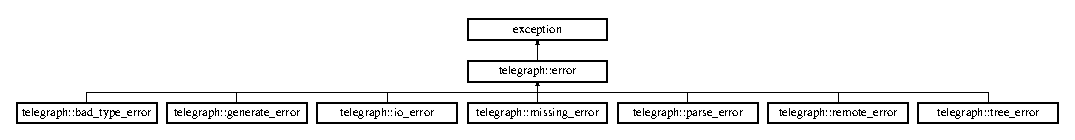
\includegraphics[height=1.437126cm]{classtelegraph_1_1error}
\end{center}
\end{figure}
\subsection*{Public Member Functions}
\begin{DoxyCompactItemize}
\item 
\hyperlink{classtelegraph_1_1error_a2381d26711bfbcb841ccd3c7e562b9f8}{error} (const std\+::string\+\_\+view \&m)
\item 
const char $\ast$ \hyperlink{classtelegraph_1_1error_acd75a8954a9d693faf75eb5918bfe044}{what} () const noexcept override
\end{DoxyCompactItemize}


\subsection{Constructor \& Destructor Documentation}
\mbox{\Hypertarget{classtelegraph_1_1error_a2381d26711bfbcb841ccd3c7e562b9f8}\label{classtelegraph_1_1error_a2381d26711bfbcb841ccd3c7e562b9f8}} 
\index{telegraph\+::error@{telegraph\+::error}!error@{error}}
\index{error@{error}!telegraph\+::error@{telegraph\+::error}}
\subsubsection{\texorpdfstring{error()}{error()}}
{\footnotesize\ttfamily telegraph\+::error\+::error (\begin{DoxyParamCaption}\item[{const std\+::string\+\_\+view \&}]{m }\end{DoxyParamCaption})\hspace{0.3cm}{\ttfamily [inline]}}



\subsection{Member Function Documentation}
\mbox{\Hypertarget{classtelegraph_1_1error_acd75a8954a9d693faf75eb5918bfe044}\label{classtelegraph_1_1error_acd75a8954a9d693faf75eb5918bfe044}} 
\index{telegraph\+::error@{telegraph\+::error}!what@{what}}
\index{what@{what}!telegraph\+::error@{telegraph\+::error}}
\subsubsection{\texorpdfstring{what()}{what()}}
{\footnotesize\ttfamily const char$\ast$ telegraph\+::error\+::what (\begin{DoxyParamCaption}{ }\end{DoxyParamCaption}) const\hspace{0.3cm}{\ttfamily [inline]}, {\ttfamily [override]}, {\ttfamily [noexcept]}}



The documentation for this class was generated from the following file\+:\begin{DoxyCompactItemize}
\item 
\hyperlink{errors_8hpp}{errors.\+hpp}\end{DoxyCompactItemize}

\hypertarget{classtelegraph_1_1forwarder}{}\section{telegraph\+:\+:forwarder Class Reference}
\label{classtelegraph_1_1forwarder}\index{telegraph\+::forwarder@{telegraph\+::forwarder}}


{\ttfamily \#include $<$forwarder.\+hpp$>$}

\subsection*{Public Member Functions}
\begin{DoxyCompactItemize}
\item 
\hyperlink{classtelegraph_1_1forwarder_abdd83232ce225a8d3f9ccd014ee5eeb2}{forwarder} (\hyperlink{classtelegraph_1_1connection}{connection} \&conn, const std\+::shared\+\_\+ptr$<$ \hyperlink{classtelegraph_1_1namespace__}{namespace\+\_\+} $>$ \&ns)
\item 
\hyperlink{classtelegraph_1_1forwarder_a61d26a7a1b8198e65824c720ab946052}{$\sim$forwarder} ()
\end{DoxyCompactItemize}


\subsection{Constructor \& Destructor Documentation}
\mbox{\Hypertarget{classtelegraph_1_1forwarder_abdd83232ce225a8d3f9ccd014ee5eeb2}\label{classtelegraph_1_1forwarder_abdd83232ce225a8d3f9ccd014ee5eeb2}} 
\index{telegraph\+::forwarder@{telegraph\+::forwarder}!forwarder@{forwarder}}
\index{forwarder@{forwarder}!telegraph\+::forwarder@{telegraph\+::forwarder}}
\subsubsection{\texorpdfstring{forwarder()}{forwarder()}}
{\footnotesize\ttfamily telegraph\+::forwarder\+::forwarder (\begin{DoxyParamCaption}\item[{\hyperlink{classtelegraph_1_1connection}{connection} \&}]{conn,  }\item[{const std\+::shared\+\_\+ptr$<$ \hyperlink{classtelegraph_1_1namespace__}{namespace\+\_\+} $>$ \&}]{ns }\end{DoxyParamCaption})}

\mbox{\Hypertarget{classtelegraph_1_1forwarder_a61d26a7a1b8198e65824c720ab946052}\label{classtelegraph_1_1forwarder_a61d26a7a1b8198e65824c720ab946052}} 
\index{telegraph\+::forwarder@{telegraph\+::forwarder}!````~forwarder@{$\sim$forwarder}}
\index{````~forwarder@{$\sim$forwarder}!telegraph\+::forwarder@{telegraph\+::forwarder}}
\subsubsection{\texorpdfstring{$\sim$forwarder()}{~forwarder()}}
{\footnotesize\ttfamily telegraph\+::forwarder\+::$\sim$forwarder (\begin{DoxyParamCaption}{ }\end{DoxyParamCaption})}



The documentation for this class was generated from the following files\+:\begin{DoxyCompactItemize}
\item 
\hyperlink{forwarder_8hpp}{forwarder.\+hpp}\item 
\hyperlink{forwarder_8cpp}{forwarder.\+cpp}\end{DoxyCompactItemize}

\hypertarget{classtelegraph_1_1generate__error}{}\section{telegraph\+:\+:generate\+\_\+error Class Reference}
\label{classtelegraph_1_1generate__error}\index{telegraph\+::generate\+\_\+error@{telegraph\+::generate\+\_\+error}}


{\ttfamily \#include $<$errors.\+hpp$>$}

Inheritance diagram for telegraph\+:\+:generate\+\_\+error\+:\begin{figure}[H]
\begin{center}
\leavevmode
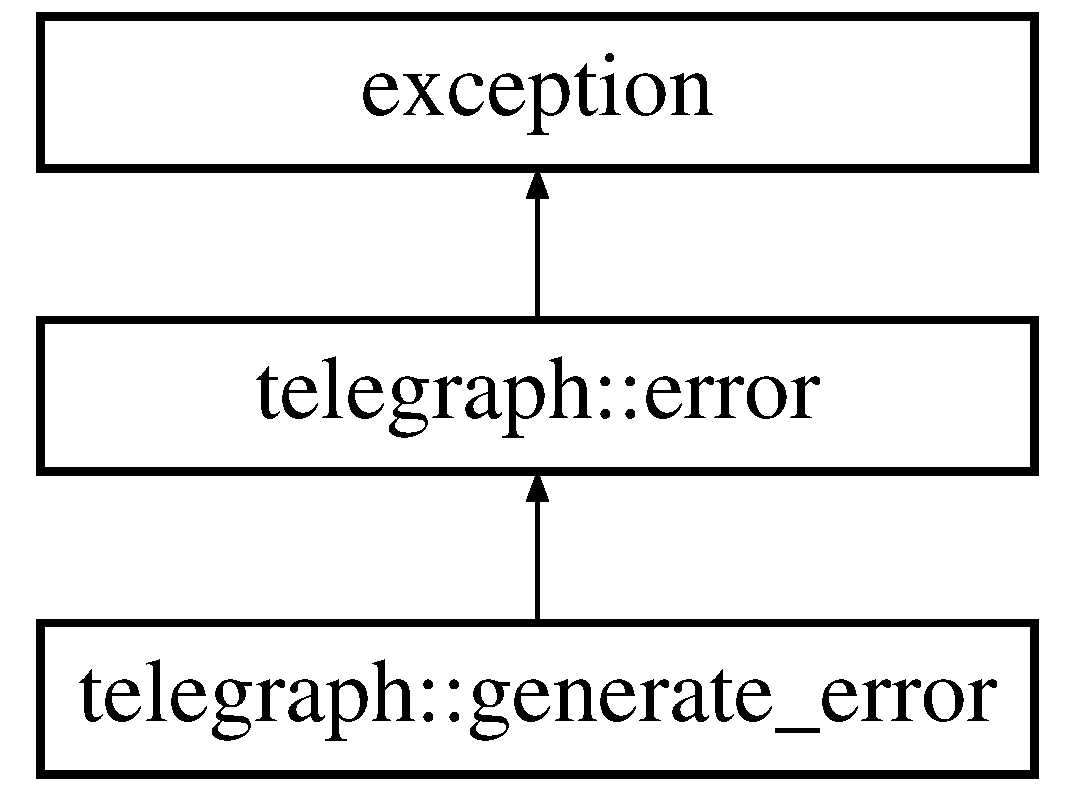
\includegraphics[height=3.000000cm]{classtelegraph_1_1generate__error}
\end{center}
\end{figure}
\subsection*{Public Member Functions}
\begin{DoxyCompactItemize}
\item 
\hyperlink{classtelegraph_1_1generate__error_aec3b4c0f38f32f0ed423e65187da0601}{generate\+\_\+error} (const std\+::string\+\_\+view \&m)
\end{DoxyCompactItemize}


\subsection{Constructor \& Destructor Documentation}
\mbox{\Hypertarget{classtelegraph_1_1generate__error_aec3b4c0f38f32f0ed423e65187da0601}\label{classtelegraph_1_1generate__error_aec3b4c0f38f32f0ed423e65187da0601}} 
\index{telegraph\+::generate\+\_\+error@{telegraph\+::generate\+\_\+error}!generate\+\_\+error@{generate\+\_\+error}}
\index{generate\+\_\+error@{generate\+\_\+error}!telegraph\+::generate\+\_\+error@{telegraph\+::generate\+\_\+error}}
\subsubsection{\texorpdfstring{generate\+\_\+error()}{generate\_error()}}
{\footnotesize\ttfamily telegraph\+::generate\+\_\+error\+::generate\+\_\+error (\begin{DoxyParamCaption}\item[{const std\+::string\+\_\+view \&}]{m }\end{DoxyParamCaption})\hspace{0.3cm}{\ttfamily [inline]}}



The documentation for this class was generated from the following file\+:\begin{DoxyCompactItemize}
\item 
\hyperlink{errors_8hpp}{errors.\+hpp}\end{DoxyCompactItemize}

\hypertarget{classtelegraph_1_1generator}{}\section{telegraph\+:\+:generator Class Reference}
\label{classtelegraph_1_1generator}\index{telegraph\+::generator@{telegraph\+::generator}}


{\ttfamily \#include $<$generator.\+hpp$>$}

\subsection*{Classes}
\begin{DoxyCompactItemize}
\item 
struct \hyperlink{structtelegraph_1_1generator_1_1result}{result}
\item 
struct \hyperlink{structtelegraph_1_1generator_1_1target}{target}
\end{DoxyCompactItemize}
\subsection*{Public Member Functions}
\begin{DoxyCompactItemize}
\item 
\hyperlink{classtelegraph_1_1generator_add831bd47c4792a2b4a2726fc13bada4}{generator} ()
\item 
void \hyperlink{classtelegraph_1_1generator_ab9540639f075db70b2763fbe7c462a94}{set\+\_\+tree} (const std\+::string \&filename, const \hyperlink{classtelegraph_1_1node}{node} $\ast$t)
\item 
void \hyperlink{classtelegraph_1_1generator_ac2e6da6fff01552c4084d27310dba3da}{set\+\_\+tree\+\_\+include} (const std\+::string \&filename, const std\+::string \&tree\+\_\+include)
\item 
void \hyperlink{classtelegraph_1_1generator_a51756531241b5bc309736fc9fc5eba39}{set\+\_\+namespace} (const std\+::string \&filename, const std\+::string \&ns)
\item 
void \hyperlink{classtelegraph_1_1generator_a7cb9bbac059ab2fca31937d2982506a8}{add\+\_\+profile} (const std\+::string \&filename, const \hyperlink{classtelegraph_1_1profile}{profile} $\ast$conf)
\item 
std\+::vector$<$ \hyperlink{structtelegraph_1_1generator_1_1result}{result} $>$ \hyperlink{classtelegraph_1_1generator_a5964a5dba70c651c616e9d5fbbcf6ca2}{generate} () const
\end{DoxyCompactItemize}


\subsection{Constructor \& Destructor Documentation}
\mbox{\Hypertarget{classtelegraph_1_1generator_add831bd47c4792a2b4a2726fc13bada4}\label{classtelegraph_1_1generator_add831bd47c4792a2b4a2726fc13bada4}} 
\index{telegraph\+::generator@{telegraph\+::generator}!generator@{generator}}
\index{generator@{generator}!telegraph\+::generator@{telegraph\+::generator}}
\subsubsection{\texorpdfstring{generator()}{generator()}}
{\footnotesize\ttfamily telegraph\+::generator\+::generator (\begin{DoxyParamCaption}{ }\end{DoxyParamCaption})}



\subsection{Member Function Documentation}
\mbox{\Hypertarget{classtelegraph_1_1generator_a7cb9bbac059ab2fca31937d2982506a8}\label{classtelegraph_1_1generator_a7cb9bbac059ab2fca31937d2982506a8}} 
\index{telegraph\+::generator@{telegraph\+::generator}!add\+\_\+profile@{add\+\_\+profile}}
\index{add\+\_\+profile@{add\+\_\+profile}!telegraph\+::generator@{telegraph\+::generator}}
\subsubsection{\texorpdfstring{add\+\_\+profile()}{add\_profile()}}
{\footnotesize\ttfamily void telegraph\+::generator\+::add\+\_\+profile (\begin{DoxyParamCaption}\item[{const std\+::string \&}]{filename,  }\item[{const \hyperlink{classtelegraph_1_1profile}{profile} $\ast$}]{conf }\end{DoxyParamCaption})}

\mbox{\Hypertarget{classtelegraph_1_1generator_a5964a5dba70c651c616e9d5fbbcf6ca2}\label{classtelegraph_1_1generator_a5964a5dba70c651c616e9d5fbbcf6ca2}} 
\index{telegraph\+::generator@{telegraph\+::generator}!generate@{generate}}
\index{generate@{generate}!telegraph\+::generator@{telegraph\+::generator}}
\subsubsection{\texorpdfstring{generate()}{generate()}}
{\footnotesize\ttfamily std\+::vector$<$ \hyperlink{structtelegraph_1_1generator_1_1result}{generator\+::result} $>$ telegraph\+::generator\+::generate (\begin{DoxyParamCaption}{ }\end{DoxyParamCaption}) const}

\mbox{\Hypertarget{classtelegraph_1_1generator_a51756531241b5bc309736fc9fc5eba39}\label{classtelegraph_1_1generator_a51756531241b5bc309736fc9fc5eba39}} 
\index{telegraph\+::generator@{telegraph\+::generator}!set\+\_\+namespace@{set\+\_\+namespace}}
\index{set\+\_\+namespace@{set\+\_\+namespace}!telegraph\+::generator@{telegraph\+::generator}}
\subsubsection{\texorpdfstring{set\+\_\+namespace()}{set\_namespace()}}
{\footnotesize\ttfamily void telegraph\+::generator\+::set\+\_\+namespace (\begin{DoxyParamCaption}\item[{const std\+::string \&}]{filename,  }\item[{const std\+::string \&}]{ns }\end{DoxyParamCaption})}

\mbox{\Hypertarget{classtelegraph_1_1generator_ab9540639f075db70b2763fbe7c462a94}\label{classtelegraph_1_1generator_ab9540639f075db70b2763fbe7c462a94}} 
\index{telegraph\+::generator@{telegraph\+::generator}!set\+\_\+tree@{set\+\_\+tree}}
\index{set\+\_\+tree@{set\+\_\+tree}!telegraph\+::generator@{telegraph\+::generator}}
\subsubsection{\texorpdfstring{set\+\_\+tree()}{set\_tree()}}
{\footnotesize\ttfamily void telegraph\+::generator\+::set\+\_\+tree (\begin{DoxyParamCaption}\item[{const std\+::string \&}]{filename,  }\item[{const \hyperlink{classtelegraph_1_1node}{node} $\ast$}]{t }\end{DoxyParamCaption})}

\mbox{\Hypertarget{classtelegraph_1_1generator_ac2e6da6fff01552c4084d27310dba3da}\label{classtelegraph_1_1generator_ac2e6da6fff01552c4084d27310dba3da}} 
\index{telegraph\+::generator@{telegraph\+::generator}!set\+\_\+tree\+\_\+include@{set\+\_\+tree\+\_\+include}}
\index{set\+\_\+tree\+\_\+include@{set\+\_\+tree\+\_\+include}!telegraph\+::generator@{telegraph\+::generator}}
\subsubsection{\texorpdfstring{set\+\_\+tree\+\_\+include()}{set\_tree\_include()}}
{\footnotesize\ttfamily void telegraph\+::generator\+::set\+\_\+tree\+\_\+include (\begin{DoxyParamCaption}\item[{const std\+::string \&}]{filename,  }\item[{const std\+::string \&}]{tree\+\_\+include }\end{DoxyParamCaption})}



The documentation for this class was generated from the following files\+:\begin{DoxyCompactItemize}
\item 
\hyperlink{generator_8hpp}{generator.\+hpp}\item 
\hyperlink{generator_8cpp}{generator.\+cpp}\end{DoxyCompactItemize}

\hypertarget{classtelegen_1_1group}{}\section{telegen\+:\+:group Class Reference}
\label{classtelegen_1_1group}\index{telegen\+::group@{telegen\+::group}}


{\ttfamily \#include $<$nodes.\+hpp$>$}

Inheritance diagram for telegen\+:\+:group\+:\begin{figure}[H]
\begin{center}
\leavevmode
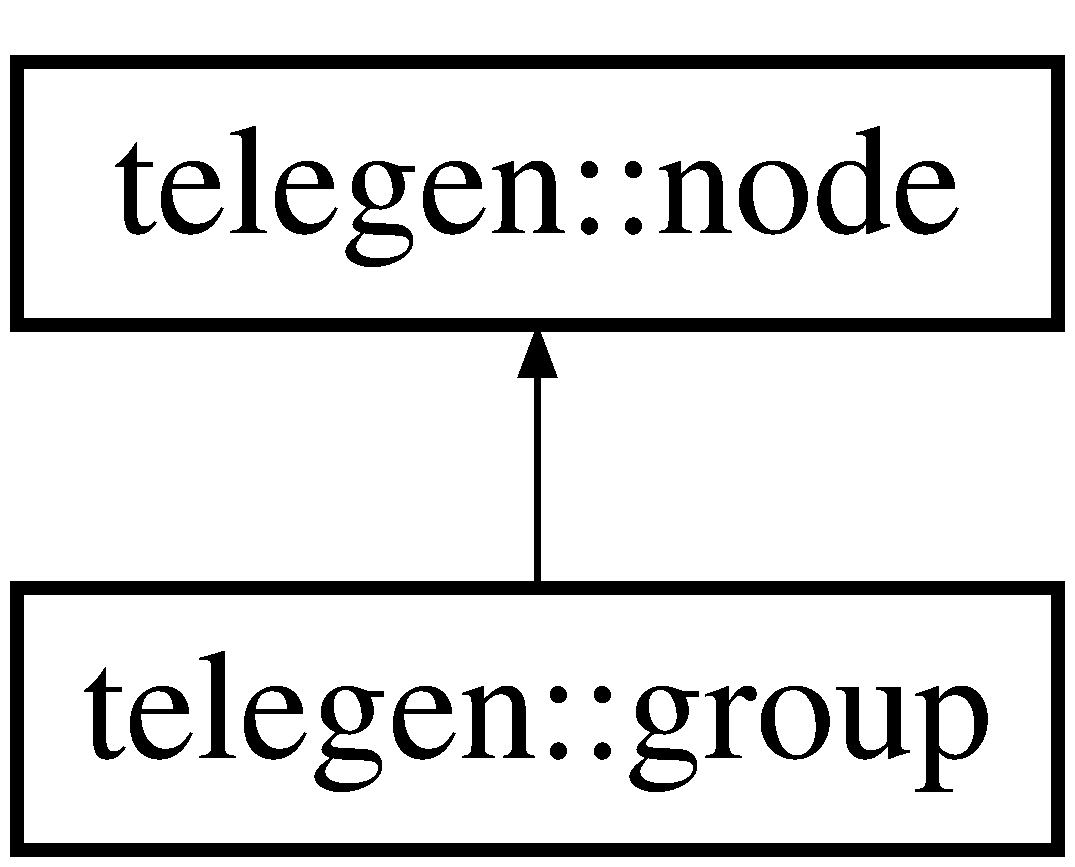
\includegraphics[height=2.000000cm]{classtelegen_1_1group}
\end{center}
\end{figure}
\subsection*{Public Member Functions}
\begin{DoxyCompactItemize}
\item 
constexpr \hyperlink{classtelegen_1_1group_aed66803b4b989a001bdafcd501d074ba}{group} (\hyperlink{classtelegen_1_1node_aae3ff0d12932c55fdc88a1743e27ea56}{id} i, const char $\ast$name, const char $\ast$pretty, const char $\ast$desc, const char $\ast$schema, int32\+\_\+t version, \hyperlink{classtelegen_1_1node}{node} $\ast$const $\ast$children, size\+\_\+t \hyperlink{classtelegen_1_1group_a499258baf8b0eb11ef802202d4385734}{num\+\_\+children})
\item 
constexpr const char $\ast$ \hyperlink{classtelegen_1_1group_ad5e61c5d1787e20921691b0ec2351396}{get\+\_\+schema} () const
\item 
constexpr int32\+\_\+t \hyperlink{classtelegen_1_1group_ad4652953e0a87d7569e4ec3ded5c2286}{get\+\_\+version} () const
\item 
constexpr size\+\_\+t \hyperlink{classtelegen_1_1group_a499258baf8b0eb11ef802202d4385734}{num\+\_\+children} () const
\item 
void \hyperlink{classtelegen_1_1group_a40efc73239b71ebaa59fe2e95f3e96a7}{pack} (telegraph\+\_\+\+Group $\ast$g) const
\item 
void \hyperlink{classtelegen_1_1group_ae146155bf745b0b3d39e3244c3ebb26d}{pack} (telegraph\+\_\+\+Node $\ast$n) const override
\end{DoxyCompactItemize}
\subsection*{Additional Inherited Members}


\subsection{Constructor \& Destructor Documentation}
\mbox{\Hypertarget{classtelegen_1_1group_aed66803b4b989a001bdafcd501d074ba}\label{classtelegen_1_1group_aed66803b4b989a001bdafcd501d074ba}} 
\index{telegen\+::group@{telegen\+::group}!group@{group}}
\index{group@{group}!telegen\+::group@{telegen\+::group}}
\subsubsection{\texorpdfstring{group()}{group()}}
{\footnotesize\ttfamily constexpr telegen\+::group\+::group (\begin{DoxyParamCaption}\item[{\hyperlink{classtelegen_1_1node_aae3ff0d12932c55fdc88a1743e27ea56}{id}}]{i,  }\item[{const char $\ast$}]{name,  }\item[{const char $\ast$}]{pretty,  }\item[{const char $\ast$}]{desc,  }\item[{const char $\ast$}]{schema,  }\item[{int32\+\_\+t}]{version,  }\item[{\hyperlink{classtelegen_1_1node}{node} $\ast$const $\ast$}]{children,  }\item[{size\+\_\+t}]{num\+\_\+children }\end{DoxyParamCaption})\hspace{0.3cm}{\ttfamily [inline]}}



\subsection{Member Function Documentation}
\mbox{\Hypertarget{classtelegen_1_1group_ad5e61c5d1787e20921691b0ec2351396}\label{classtelegen_1_1group_ad5e61c5d1787e20921691b0ec2351396}} 
\index{telegen\+::group@{telegen\+::group}!get\+\_\+schema@{get\+\_\+schema}}
\index{get\+\_\+schema@{get\+\_\+schema}!telegen\+::group@{telegen\+::group}}
\subsubsection{\texorpdfstring{get\+\_\+schema()}{get\_schema()}}
{\footnotesize\ttfamily constexpr const char$\ast$ telegen\+::group\+::get\+\_\+schema (\begin{DoxyParamCaption}{ }\end{DoxyParamCaption}) const\hspace{0.3cm}{\ttfamily [inline]}}

\mbox{\Hypertarget{classtelegen_1_1group_ad4652953e0a87d7569e4ec3ded5c2286}\label{classtelegen_1_1group_ad4652953e0a87d7569e4ec3ded5c2286}} 
\index{telegen\+::group@{telegen\+::group}!get\+\_\+version@{get\+\_\+version}}
\index{get\+\_\+version@{get\+\_\+version}!telegen\+::group@{telegen\+::group}}
\subsubsection{\texorpdfstring{get\+\_\+version()}{get\_version()}}
{\footnotesize\ttfamily constexpr int32\+\_\+t telegen\+::group\+::get\+\_\+version (\begin{DoxyParamCaption}{ }\end{DoxyParamCaption}) const\hspace{0.3cm}{\ttfamily [inline]}}

\mbox{\Hypertarget{classtelegen_1_1group_a499258baf8b0eb11ef802202d4385734}\label{classtelegen_1_1group_a499258baf8b0eb11ef802202d4385734}} 
\index{telegen\+::group@{telegen\+::group}!num\+\_\+children@{num\+\_\+children}}
\index{num\+\_\+children@{num\+\_\+children}!telegen\+::group@{telegen\+::group}}
\subsubsection{\texorpdfstring{num\+\_\+children()}{num\_children()}}
{\footnotesize\ttfamily constexpr size\+\_\+t telegen\+::group\+::num\+\_\+children (\begin{DoxyParamCaption}{ }\end{DoxyParamCaption}) const\hspace{0.3cm}{\ttfamily [inline]}}

\mbox{\Hypertarget{classtelegen_1_1group_a40efc73239b71ebaa59fe2e95f3e96a7}\label{classtelegen_1_1group_a40efc73239b71ebaa59fe2e95f3e96a7}} 
\index{telegen\+::group@{telegen\+::group}!pack@{pack}}
\index{pack@{pack}!telegen\+::group@{telegen\+::group}}
\subsubsection{\texorpdfstring{pack()}{pack()}\hspace{0.1cm}{\footnotesize\ttfamily [1/2]}}
{\footnotesize\ttfamily void telegen\+::group\+::pack (\begin{DoxyParamCaption}\item[{telegraph\+\_\+\+Group $\ast$}]{g }\end{DoxyParamCaption}) const\hspace{0.3cm}{\ttfamily [inline]}}

\mbox{\Hypertarget{classtelegen_1_1group_ae146155bf745b0b3d39e3244c3ebb26d}\label{classtelegen_1_1group_ae146155bf745b0b3d39e3244c3ebb26d}} 
\index{telegen\+::group@{telegen\+::group}!pack@{pack}}
\index{pack@{pack}!telegen\+::group@{telegen\+::group}}
\subsubsection{\texorpdfstring{pack()}{pack()}\hspace{0.1cm}{\footnotesize\ttfamily [2/2]}}
{\footnotesize\ttfamily void telegen\+::group\+::pack (\begin{DoxyParamCaption}\item[{telegraph\+\_\+\+Node $\ast$}]{n }\end{DoxyParamCaption}) const\hspace{0.3cm}{\ttfamily [inline]}, {\ttfamily [override]}, {\ttfamily [virtual]}}



Implements \hyperlink{classtelegen_1_1node_a8b6169d62f6e7c2e301435e52442fed3}{telegen\+::node}.



The documentation for this class was generated from the following file\+:\begin{DoxyCompactItemize}
\item 
\hyperlink{gen_2telegen_2nodes_8hpp}{gen/telegen/nodes.\+hpp}\end{DoxyCompactItemize}

\hypertarget{classtelegraph_1_1group}{}\section{telegraph\+:\+:group Class Reference}
\label{classtelegraph_1_1group}\index{telegraph\+::group@{telegraph\+::group}}


{\ttfamily \#include $<$nodes.\+hpp$>$}

Inheritance diagram for telegraph\+:\+:group\+:\begin{figure}[H]
\begin{center}
\leavevmode
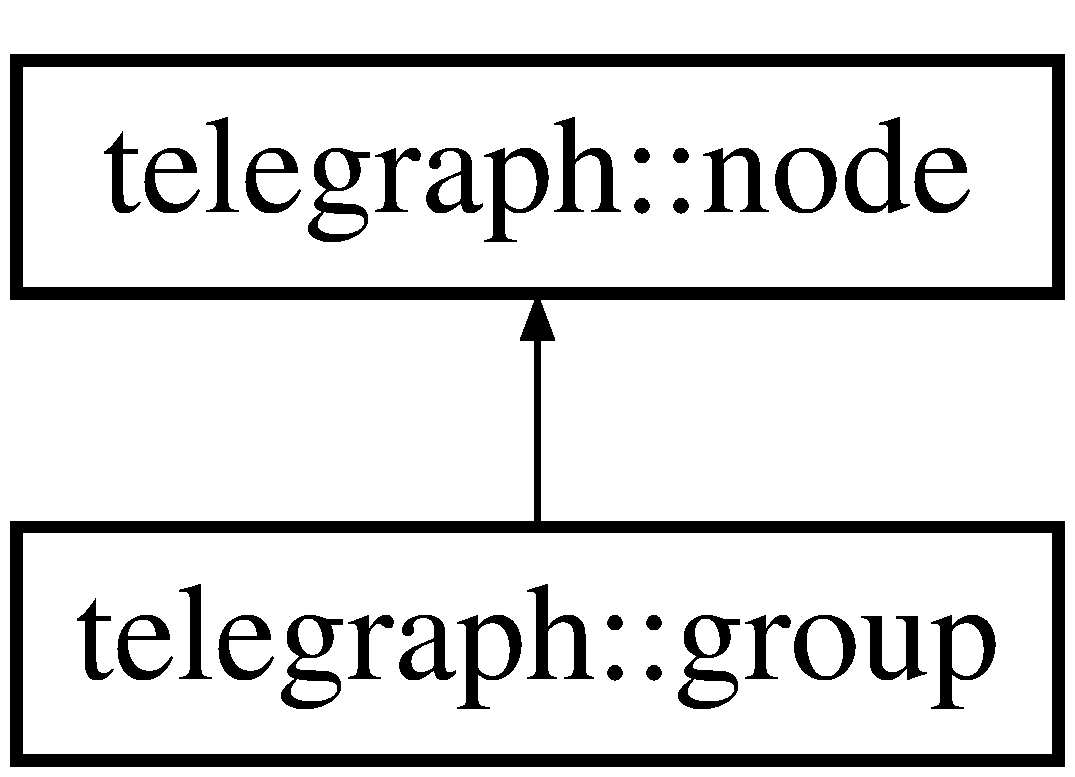
\includegraphics[height=2.000000cm]{classtelegraph_1_1group}
\end{center}
\end{figure}
\subsection*{Public Member Functions}
\begin{DoxyCompactItemize}
\item 
\hyperlink{classtelegraph_1_1group_a06ec96e471690fcc8e9cc6efe1632261}{group} (\hyperlink{classtelegraph_1_1node_a90bc576d668ed141d5354a06aa9c8d9a}{id} i, const std\+::string\+\_\+view \&name, const std\+::string\+\_\+view \&pretty, const std\+::string\+\_\+view \&desc, const std\+::string\+\_\+view \&schema, int version, std\+::vector$<$ \hyperlink{classtelegraph_1_1node}{node} $\ast$$>$ \&\&children)
\item 
\hyperlink{classtelegraph_1_1group_a88d584b6dc7383e319a00fc266b29be7}{group} (const \hyperlink{classtelegraph_1_1group}{group} \&g)
\item 
\hyperlink{classtelegraph_1_1group_a2c613f213d32b7b48b94df99610bbc90}{$\sim$group} ()
\item 
const std\+::string \& \hyperlink{classtelegraph_1_1group_a6ab1978bc6c97d3dcd802665c92390b8}{get\+\_\+schema} () const
\item 
int \hyperlink{classtelegraph_1_1group_a04e3ffe2ee3b18f0c2d921bdd8b0789f}{get\+\_\+version} () const
\item 
void \hyperlink{classtelegraph_1_1group_ae4887f80cadba073aef9feef1295fb20}{set\+\_\+owner} (const std\+::weak\+\_\+ptr$<$ \hyperlink{classtelegraph_1_1context}{context} $>$ \&c) override
\item 
void \hyperlink{classtelegraph_1_1group_af56fb03ad97aadd9be32c5e47c6d195b}{set\+\_\+unowned} () override
\item 
\hyperlink{classtelegraph_1_1node}{node} $\ast$ \hyperlink{classtelegraph_1_1group_a27e8f2ecfe0b87fef8ca57c43fda8809}{from\+\_\+path} (const std\+::vector$<$ std\+::string\+\_\+view $>$ \&p, size\+\_\+t idx=0) override
\item 
const \hyperlink{classtelegraph_1_1node}{node} $\ast$ \hyperlink{classtelegraph_1_1group_ad4ed6177fee328ec3702d01a881a33ee}{from\+\_\+path} (const std\+::vector$<$ std\+::string\+\_\+view $>$ \&p, size\+\_\+t idx=0) const override
\item 
std\+::vector$<$ \hyperlink{classtelegraph_1_1node}{node} $\ast$ $>$ \hyperlink{classtelegraph_1_1group_a120c05f05d045fe4b5719b4abe4e83d9}{nodes} () override
\item 
std\+::vector$<$ const \hyperlink{classtelegraph_1_1node}{node} $\ast$ $>$ \hyperlink{classtelegraph_1_1group_ad5a82543eef530a7b07ca2cdbe6a82f5}{nodes} () const override
\item 
\hyperlink{classtelegraph_1_1node}{node} $\ast$ \hyperlink{classtelegraph_1_1group_aaf32eea781de1f18d37765793589dda5}{operator\mbox{[}$\,$\mbox{]}} (size\+\_\+t idx) override
\item 
const \hyperlink{classtelegraph_1_1node}{node} $\ast$ \hyperlink{classtelegraph_1_1group_a1b084997076f624d3814b057b26162cd}{operator\mbox{[}$\,$\mbox{]}} (size\+\_\+t idx) const override
\item 
\hyperlink{classtelegraph_1_1node}{node} $\ast$ \hyperlink{classtelegraph_1_1group_a84db0dc9c8d45bdd343a0d4da44a3593}{operator\mbox{[}$\,$\mbox{]}} (const std\+::string \&child) override
\item 
const \hyperlink{classtelegraph_1_1node}{node} $\ast$ \hyperlink{classtelegraph_1_1group_abc407505a0b1d0f1c3de0f588f8ea7a0}{operator\mbox{[}$\,$\mbox{]}} (const std\+::string \&child) const override
\item 
std\+::vector$<$ \hyperlink{classtelegraph_1_1node}{node} $\ast$ $>$\+::iterator \hyperlink{classtelegraph_1_1group_a71c8576e9cf6035fd371516b1e1fc692}{begin} ()
\item 
std\+::vector$<$ \hyperlink{classtelegraph_1_1node}{node} $\ast$ $>$\+::const\+\_\+iterator \hyperlink{classtelegraph_1_1group_a0ec680f2044108436dbecc8f25b2cba6}{begin} () const
\item 
std\+::vector$<$ \hyperlink{classtelegraph_1_1node}{node} $\ast$ $>$\+::iterator \hyperlink{classtelegraph_1_1group_afe980e1a055ebba5eb236cf09738bad8}{end} ()
\item 
std\+::vector$<$ \hyperlink{classtelegraph_1_1node}{node} $\ast$ $>$\+::const\+\_\+iterator \hyperlink{classtelegraph_1_1group_ab06ca45e8bd109f94d2ea763c92de677}{end} () const
\item 
size\+\_\+t \hyperlink{classtelegraph_1_1group_a75e3d657ee7458aeedfcc353bd50e571}{num\+\_\+children} () const
\item 
bool \hyperlink{classtelegraph_1_1group_a63cf8362b39b718e9553a519485f7875}{compatible\+\_\+with} (\hyperlink{classtelegraph_1_1node}{node} $\ast$other) const override
\item 
void \hyperlink{classtelegraph_1_1group_a2899f0bebaa9696675c7a32fd92d54e9}{pack} (Group $\ast$\hyperlink{classtelegraph_1_1group}{group}) const
\item 
virtual void \hyperlink{classtelegraph_1_1group_a070decfe980bb669646af5307f5c93e4}{pack} (Node $\ast$proto) const override
\item 
std\+::unique\+\_\+ptr$<$ \hyperlink{classtelegraph_1_1node}{node} $>$ \hyperlink{classtelegraph_1_1group_a0e937eea18e4f650b892ac9061c461fa}{clone} () const override
\end{DoxyCompactItemize}
\subsection*{Static Public Member Functions}
\begin{DoxyCompactItemize}
\item 
static \hyperlink{classtelegraph_1_1group}{group} $\ast$ \hyperlink{classtelegraph_1_1group_a92934fab7dc94207f4d98a40deef0f55}{unpack} (const Group \&g)
\end{DoxyCompactItemize}
\subsection*{Additional Inherited Members}


\subsection{Constructor \& Destructor Documentation}
\mbox{\Hypertarget{classtelegraph_1_1group_a06ec96e471690fcc8e9cc6efe1632261}\label{classtelegraph_1_1group_a06ec96e471690fcc8e9cc6efe1632261}} 
\index{telegraph\+::group@{telegraph\+::group}!group@{group}}
\index{group@{group}!telegraph\+::group@{telegraph\+::group}}
\subsubsection{\texorpdfstring{group()}{group()}\hspace{0.1cm}{\footnotesize\ttfamily [1/2]}}
{\footnotesize\ttfamily telegraph\+::group\+::group (\begin{DoxyParamCaption}\item[{\hyperlink{classtelegraph_1_1node_a90bc576d668ed141d5354a06aa9c8d9a}{id}}]{i,  }\item[{const std\+::string\+\_\+view \&}]{name,  }\item[{const std\+::string\+\_\+view \&}]{pretty,  }\item[{const std\+::string\+\_\+view \&}]{desc,  }\item[{const std\+::string\+\_\+view \&}]{schema,  }\item[{int}]{version,  }\item[{std\+::vector$<$ \hyperlink{classtelegraph_1_1node}{node} $\ast$$>$ \&\&}]{children }\end{DoxyParamCaption})\hspace{0.3cm}{\ttfamily [inline]}}

\mbox{\Hypertarget{classtelegraph_1_1group_a88d584b6dc7383e319a00fc266b29be7}\label{classtelegraph_1_1group_a88d584b6dc7383e319a00fc266b29be7}} 
\index{telegraph\+::group@{telegraph\+::group}!group@{group}}
\index{group@{group}!telegraph\+::group@{telegraph\+::group}}
\subsubsection{\texorpdfstring{group()}{group()}\hspace{0.1cm}{\footnotesize\ttfamily [2/2]}}
{\footnotesize\ttfamily telegraph\+::group\+::group (\begin{DoxyParamCaption}\item[{const \hyperlink{classtelegraph_1_1group}{group} \&}]{g }\end{DoxyParamCaption})\hspace{0.3cm}{\ttfamily [inline]}}

\mbox{\Hypertarget{classtelegraph_1_1group_a2c613f213d32b7b48b94df99610bbc90}\label{classtelegraph_1_1group_a2c613f213d32b7b48b94df99610bbc90}} 
\index{telegraph\+::group@{telegraph\+::group}!````~group@{$\sim$group}}
\index{````~group@{$\sim$group}!telegraph\+::group@{telegraph\+::group}}
\subsubsection{\texorpdfstring{$\sim$group()}{~group()}}
{\footnotesize\ttfamily telegraph\+::group\+::$\sim$group (\begin{DoxyParamCaption}{ }\end{DoxyParamCaption})\hspace{0.3cm}{\ttfamily [inline]}}



\subsection{Member Function Documentation}
\mbox{\Hypertarget{classtelegraph_1_1group_a71c8576e9cf6035fd371516b1e1fc692}\label{classtelegraph_1_1group_a71c8576e9cf6035fd371516b1e1fc692}} 
\index{telegraph\+::group@{telegraph\+::group}!begin@{begin}}
\index{begin@{begin}!telegraph\+::group@{telegraph\+::group}}
\subsubsection{\texorpdfstring{begin()}{begin()}\hspace{0.1cm}{\footnotesize\ttfamily [1/2]}}
{\footnotesize\ttfamily std\+::vector$<$\hyperlink{classtelegraph_1_1node}{node}$\ast$$>$\+::iterator telegraph\+::group\+::begin (\begin{DoxyParamCaption}{ }\end{DoxyParamCaption})\hspace{0.3cm}{\ttfamily [inline]}}

\mbox{\Hypertarget{classtelegraph_1_1group_a0ec680f2044108436dbecc8f25b2cba6}\label{classtelegraph_1_1group_a0ec680f2044108436dbecc8f25b2cba6}} 
\index{telegraph\+::group@{telegraph\+::group}!begin@{begin}}
\index{begin@{begin}!telegraph\+::group@{telegraph\+::group}}
\subsubsection{\texorpdfstring{begin()}{begin()}\hspace{0.1cm}{\footnotesize\ttfamily [2/2]}}
{\footnotesize\ttfamily std\+::vector$<$\hyperlink{classtelegraph_1_1node}{node}$\ast$$>$\+::const\+\_\+iterator telegraph\+::group\+::begin (\begin{DoxyParamCaption}{ }\end{DoxyParamCaption}) const\hspace{0.3cm}{\ttfamily [inline]}}

\mbox{\Hypertarget{classtelegraph_1_1group_a0e937eea18e4f650b892ac9061c461fa}\label{classtelegraph_1_1group_a0e937eea18e4f650b892ac9061c461fa}} 
\index{telegraph\+::group@{telegraph\+::group}!clone@{clone}}
\index{clone@{clone}!telegraph\+::group@{telegraph\+::group}}
\subsubsection{\texorpdfstring{clone()}{clone()}}
{\footnotesize\ttfamily std\+::unique\+\_\+ptr$<$\hyperlink{classtelegraph_1_1node}{node}$>$ telegraph\+::group\+::clone (\begin{DoxyParamCaption}{ }\end{DoxyParamCaption}) const\hspace{0.3cm}{\ttfamily [inline]}, {\ttfamily [override]}, {\ttfamily [virtual]}}



Implements \hyperlink{classtelegraph_1_1node_ae90515f4573cfa43c168cba9d542df6b}{telegraph\+::node}.

\mbox{\Hypertarget{classtelegraph_1_1group_a63cf8362b39b718e9553a519485f7875}\label{classtelegraph_1_1group_a63cf8362b39b718e9553a519485f7875}} 
\index{telegraph\+::group@{telegraph\+::group}!compatible\+\_\+with@{compatible\+\_\+with}}
\index{compatible\+\_\+with@{compatible\+\_\+with}!telegraph\+::group@{telegraph\+::group}}
\subsubsection{\texorpdfstring{compatible\+\_\+with()}{compatible\_with()}}
{\footnotesize\ttfamily bool telegraph\+::group\+::compatible\+\_\+with (\begin{DoxyParamCaption}\item[{\hyperlink{classtelegraph_1_1node}{node} $\ast$}]{other }\end{DoxyParamCaption}) const\hspace{0.3cm}{\ttfamily [override]}, {\ttfamily [virtual]}}



Implements \hyperlink{classtelegraph_1_1node_a68c4aed1434da1f0ece9089ff99ffcdb}{telegraph\+::node}.

\mbox{\Hypertarget{classtelegraph_1_1group_afe980e1a055ebba5eb236cf09738bad8}\label{classtelegraph_1_1group_afe980e1a055ebba5eb236cf09738bad8}} 
\index{telegraph\+::group@{telegraph\+::group}!end@{end}}
\index{end@{end}!telegraph\+::group@{telegraph\+::group}}
\subsubsection{\texorpdfstring{end()}{end()}\hspace{0.1cm}{\footnotesize\ttfamily [1/2]}}
{\footnotesize\ttfamily std\+::vector$<$\hyperlink{classtelegraph_1_1node}{node}$\ast$$>$\+::iterator telegraph\+::group\+::end (\begin{DoxyParamCaption}{ }\end{DoxyParamCaption})\hspace{0.3cm}{\ttfamily [inline]}}

\mbox{\Hypertarget{classtelegraph_1_1group_ab06ca45e8bd109f94d2ea763c92de677}\label{classtelegraph_1_1group_ab06ca45e8bd109f94d2ea763c92de677}} 
\index{telegraph\+::group@{telegraph\+::group}!end@{end}}
\index{end@{end}!telegraph\+::group@{telegraph\+::group}}
\subsubsection{\texorpdfstring{end()}{end()}\hspace{0.1cm}{\footnotesize\ttfamily [2/2]}}
{\footnotesize\ttfamily std\+::vector$<$\hyperlink{classtelegraph_1_1node}{node}$\ast$$>$\+::const\+\_\+iterator telegraph\+::group\+::end (\begin{DoxyParamCaption}{ }\end{DoxyParamCaption}) const\hspace{0.3cm}{\ttfamily [inline]}}

\mbox{\Hypertarget{classtelegraph_1_1group_a27e8f2ecfe0b87fef8ca57c43fda8809}\label{classtelegraph_1_1group_a27e8f2ecfe0b87fef8ca57c43fda8809}} 
\index{telegraph\+::group@{telegraph\+::group}!from\+\_\+path@{from\+\_\+path}}
\index{from\+\_\+path@{from\+\_\+path}!telegraph\+::group@{telegraph\+::group}}
\subsubsection{\texorpdfstring{from\+\_\+path()}{from\_path()}\hspace{0.1cm}{\footnotesize\ttfamily [1/2]}}
{\footnotesize\ttfamily \hyperlink{classtelegraph_1_1node}{node}$\ast$ telegraph\+::group\+::from\+\_\+path (\begin{DoxyParamCaption}\item[{const std\+::vector$<$ std\+::string\+\_\+view $>$ \&}]{p,  }\item[{size\+\_\+t}]{idx = {\ttfamily 0} }\end{DoxyParamCaption})\hspace{0.3cm}{\ttfamily [inline]}, {\ttfamily [override]}, {\ttfamily [virtual]}}



Reimplemented from \hyperlink{classtelegraph_1_1node_a2d5ea5366a04f3b3841de9bc21e70416}{telegraph\+::node}.

\mbox{\Hypertarget{classtelegraph_1_1group_ad4ed6177fee328ec3702d01a881a33ee}\label{classtelegraph_1_1group_ad4ed6177fee328ec3702d01a881a33ee}} 
\index{telegraph\+::group@{telegraph\+::group}!from\+\_\+path@{from\+\_\+path}}
\index{from\+\_\+path@{from\+\_\+path}!telegraph\+::group@{telegraph\+::group}}
\subsubsection{\texorpdfstring{from\+\_\+path()}{from\_path()}\hspace{0.1cm}{\footnotesize\ttfamily [2/2]}}
{\footnotesize\ttfamily const \hyperlink{classtelegraph_1_1node}{node}$\ast$ telegraph\+::group\+::from\+\_\+path (\begin{DoxyParamCaption}\item[{const std\+::vector$<$ std\+::string\+\_\+view $>$ \&}]{p,  }\item[{size\+\_\+t}]{idx = {\ttfamily 0} }\end{DoxyParamCaption}) const\hspace{0.3cm}{\ttfamily [inline]}, {\ttfamily [override]}, {\ttfamily [virtual]}}



Reimplemented from \hyperlink{classtelegraph_1_1node_aaba33e2aa28a99dcd8f4b1888c3a5706}{telegraph\+::node}.

\mbox{\Hypertarget{classtelegraph_1_1group_a6ab1978bc6c97d3dcd802665c92390b8}\label{classtelegraph_1_1group_a6ab1978bc6c97d3dcd802665c92390b8}} 
\index{telegraph\+::group@{telegraph\+::group}!get\+\_\+schema@{get\+\_\+schema}}
\index{get\+\_\+schema@{get\+\_\+schema}!telegraph\+::group@{telegraph\+::group}}
\subsubsection{\texorpdfstring{get\+\_\+schema()}{get\_schema()}}
{\footnotesize\ttfamily const std\+::string\& telegraph\+::group\+::get\+\_\+schema (\begin{DoxyParamCaption}{ }\end{DoxyParamCaption}) const\hspace{0.3cm}{\ttfamily [inline]}}

\mbox{\Hypertarget{classtelegraph_1_1group_a04e3ffe2ee3b18f0c2d921bdd8b0789f}\label{classtelegraph_1_1group_a04e3ffe2ee3b18f0c2d921bdd8b0789f}} 
\index{telegraph\+::group@{telegraph\+::group}!get\+\_\+version@{get\+\_\+version}}
\index{get\+\_\+version@{get\+\_\+version}!telegraph\+::group@{telegraph\+::group}}
\subsubsection{\texorpdfstring{get\+\_\+version()}{get\_version()}}
{\footnotesize\ttfamily int telegraph\+::group\+::get\+\_\+version (\begin{DoxyParamCaption}{ }\end{DoxyParamCaption}) const\hspace{0.3cm}{\ttfamily [inline]}}

\mbox{\Hypertarget{classtelegraph_1_1group_a120c05f05d045fe4b5719b4abe4e83d9}\label{classtelegraph_1_1group_a120c05f05d045fe4b5719b4abe4e83d9}} 
\index{telegraph\+::group@{telegraph\+::group}!nodes@{nodes}}
\index{nodes@{nodes}!telegraph\+::group@{telegraph\+::group}}
\subsubsection{\texorpdfstring{nodes()}{nodes()}\hspace{0.1cm}{\footnotesize\ttfamily [1/2]}}
{\footnotesize\ttfamily std\+::vector$<$\hyperlink{classtelegraph_1_1node}{node}$\ast$$>$ telegraph\+::group\+::nodes (\begin{DoxyParamCaption}{ }\end{DoxyParamCaption})\hspace{0.3cm}{\ttfamily [inline]}, {\ttfamily [override]}, {\ttfamily [virtual]}}



Reimplemented from \hyperlink{classtelegraph_1_1node_a14eb2051c1efaf4de6684d3e50aebeb7}{telegraph\+::node}.

\mbox{\Hypertarget{classtelegraph_1_1group_ad5a82543eef530a7b07ca2cdbe6a82f5}\label{classtelegraph_1_1group_ad5a82543eef530a7b07ca2cdbe6a82f5}} 
\index{telegraph\+::group@{telegraph\+::group}!nodes@{nodes}}
\index{nodes@{nodes}!telegraph\+::group@{telegraph\+::group}}
\subsubsection{\texorpdfstring{nodes()}{nodes()}\hspace{0.1cm}{\footnotesize\ttfamily [2/2]}}
{\footnotesize\ttfamily std\+::vector$<$const \hyperlink{classtelegraph_1_1node}{node}$\ast$$>$ telegraph\+::group\+::nodes (\begin{DoxyParamCaption}{ }\end{DoxyParamCaption}) const\hspace{0.3cm}{\ttfamily [inline]}, {\ttfamily [override]}, {\ttfamily [virtual]}}



Reimplemented from \hyperlink{classtelegraph_1_1node_a9d19888a9a73a4623dcab55be6386395}{telegraph\+::node}.

\mbox{\Hypertarget{classtelegraph_1_1group_a75e3d657ee7458aeedfcc353bd50e571}\label{classtelegraph_1_1group_a75e3d657ee7458aeedfcc353bd50e571}} 
\index{telegraph\+::group@{telegraph\+::group}!num\+\_\+children@{num\+\_\+children}}
\index{num\+\_\+children@{num\+\_\+children}!telegraph\+::group@{telegraph\+::group}}
\subsubsection{\texorpdfstring{num\+\_\+children()}{num\_children()}}
{\footnotesize\ttfamily size\+\_\+t telegraph\+::group\+::num\+\_\+children (\begin{DoxyParamCaption}{ }\end{DoxyParamCaption}) const\hspace{0.3cm}{\ttfamily [inline]}}

\mbox{\Hypertarget{classtelegraph_1_1group_aaf32eea781de1f18d37765793589dda5}\label{classtelegraph_1_1group_aaf32eea781de1f18d37765793589dda5}} 
\index{telegraph\+::group@{telegraph\+::group}!operator\mbox{[}\mbox{]}@{operator[]}}
\index{operator\mbox{[}\mbox{]}@{operator[]}!telegraph\+::group@{telegraph\+::group}}
\subsubsection{\texorpdfstring{operator[]()}{operator[]()}\hspace{0.1cm}{\footnotesize\ttfamily [1/4]}}
{\footnotesize\ttfamily \hyperlink{classtelegraph_1_1node}{node}$\ast$ telegraph\+::group\+::operator\mbox{[}$\,$\mbox{]} (\begin{DoxyParamCaption}\item[{size\+\_\+t}]{idx }\end{DoxyParamCaption})\hspace{0.3cm}{\ttfamily [inline]}, {\ttfamily [override]}, {\ttfamily [virtual]}}



Reimplemented from \hyperlink{classtelegraph_1_1node_ad82c9a9af7b7cf132db1c1e74f09254f}{telegraph\+::node}.

\mbox{\Hypertarget{classtelegraph_1_1group_a1b084997076f624d3814b057b26162cd}\label{classtelegraph_1_1group_a1b084997076f624d3814b057b26162cd}} 
\index{telegraph\+::group@{telegraph\+::group}!operator\mbox{[}\mbox{]}@{operator[]}}
\index{operator\mbox{[}\mbox{]}@{operator[]}!telegraph\+::group@{telegraph\+::group}}
\subsubsection{\texorpdfstring{operator[]()}{operator[]()}\hspace{0.1cm}{\footnotesize\ttfamily [2/4]}}
{\footnotesize\ttfamily const \hyperlink{classtelegraph_1_1node}{node}$\ast$ telegraph\+::group\+::operator\mbox{[}$\,$\mbox{]} (\begin{DoxyParamCaption}\item[{size\+\_\+t}]{idx }\end{DoxyParamCaption}) const\hspace{0.3cm}{\ttfamily [inline]}, {\ttfamily [override]}, {\ttfamily [virtual]}}



Reimplemented from \hyperlink{classtelegraph_1_1node_a4a2a451694b0a4b2c4ec26eee02e46ad}{telegraph\+::node}.

\mbox{\Hypertarget{classtelegraph_1_1group_a84db0dc9c8d45bdd343a0d4da44a3593}\label{classtelegraph_1_1group_a84db0dc9c8d45bdd343a0d4da44a3593}} 
\index{telegraph\+::group@{telegraph\+::group}!operator\mbox{[}\mbox{]}@{operator[]}}
\index{operator\mbox{[}\mbox{]}@{operator[]}!telegraph\+::group@{telegraph\+::group}}
\subsubsection{\texorpdfstring{operator[]()}{operator[]()}\hspace{0.1cm}{\footnotesize\ttfamily [3/4]}}
{\footnotesize\ttfamily \hyperlink{classtelegraph_1_1node}{node}$\ast$ telegraph\+::group\+::operator\mbox{[}$\,$\mbox{]} (\begin{DoxyParamCaption}\item[{const std\+::string \&}]{child }\end{DoxyParamCaption})\hspace{0.3cm}{\ttfamily [inline]}, {\ttfamily [override]}, {\ttfamily [virtual]}}



Reimplemented from \hyperlink{classtelegraph_1_1node_a3cf657c57fe639f6288f2acdd9b50e3c}{telegraph\+::node}.

\mbox{\Hypertarget{classtelegraph_1_1group_abc407505a0b1d0f1c3de0f588f8ea7a0}\label{classtelegraph_1_1group_abc407505a0b1d0f1c3de0f588f8ea7a0}} 
\index{telegraph\+::group@{telegraph\+::group}!operator\mbox{[}\mbox{]}@{operator[]}}
\index{operator\mbox{[}\mbox{]}@{operator[]}!telegraph\+::group@{telegraph\+::group}}
\subsubsection{\texorpdfstring{operator[]()}{operator[]()}\hspace{0.1cm}{\footnotesize\ttfamily [4/4]}}
{\footnotesize\ttfamily const \hyperlink{classtelegraph_1_1node}{node}$\ast$ telegraph\+::group\+::operator\mbox{[}$\,$\mbox{]} (\begin{DoxyParamCaption}\item[{const std\+::string \&}]{child }\end{DoxyParamCaption}) const\hspace{0.3cm}{\ttfamily [inline]}, {\ttfamily [override]}, {\ttfamily [virtual]}}



Reimplemented from \hyperlink{classtelegraph_1_1node_aad6b0bbccc9831f82117a1cc03493f6c}{telegraph\+::node}.

\mbox{\Hypertarget{classtelegraph_1_1group_a2899f0bebaa9696675c7a32fd92d54e9}\label{classtelegraph_1_1group_a2899f0bebaa9696675c7a32fd92d54e9}} 
\index{telegraph\+::group@{telegraph\+::group}!pack@{pack}}
\index{pack@{pack}!telegraph\+::group@{telegraph\+::group}}
\subsubsection{\texorpdfstring{pack()}{pack()}\hspace{0.1cm}{\footnotesize\ttfamily [1/2]}}
{\footnotesize\ttfamily void telegraph\+::group\+::pack (\begin{DoxyParamCaption}\item[{Group $\ast$}]{group }\end{DoxyParamCaption}) const}

\mbox{\Hypertarget{classtelegraph_1_1group_a070decfe980bb669646af5307f5c93e4}\label{classtelegraph_1_1group_a070decfe980bb669646af5307f5c93e4}} 
\index{telegraph\+::group@{telegraph\+::group}!pack@{pack}}
\index{pack@{pack}!telegraph\+::group@{telegraph\+::group}}
\subsubsection{\texorpdfstring{pack()}{pack()}\hspace{0.1cm}{\footnotesize\ttfamily [2/2]}}
{\footnotesize\ttfamily void telegraph\+::group\+::pack (\begin{DoxyParamCaption}\item[{Node $\ast$}]{proto }\end{DoxyParamCaption}) const\hspace{0.3cm}{\ttfamily [override]}, {\ttfamily [virtual]}}



Implements \hyperlink{classtelegraph_1_1node_a5006b21e9b83ecd52f3f953a1b828773}{telegraph\+::node}.

\mbox{\Hypertarget{classtelegraph_1_1group_ae4887f80cadba073aef9feef1295fb20}\label{classtelegraph_1_1group_ae4887f80cadba073aef9feef1295fb20}} 
\index{telegraph\+::group@{telegraph\+::group}!set\+\_\+owner@{set\+\_\+owner}}
\index{set\+\_\+owner@{set\+\_\+owner}!telegraph\+::group@{telegraph\+::group}}
\subsubsection{\texorpdfstring{set\+\_\+owner()}{set\_owner()}}
{\footnotesize\ttfamily void telegraph\+::group\+::set\+\_\+owner (\begin{DoxyParamCaption}\item[{const std\+::weak\+\_\+ptr$<$ \hyperlink{classtelegraph_1_1context}{context} $>$ \&}]{c }\end{DoxyParamCaption})\hspace{0.3cm}{\ttfamily [inline]}, {\ttfamily [override]}, {\ttfamily [virtual]}}



Reimplemented from \hyperlink{classtelegraph_1_1node_a6d864584bfadd3520194066f8b62812b}{telegraph\+::node}.

\mbox{\Hypertarget{classtelegraph_1_1group_af56fb03ad97aadd9be32c5e47c6d195b}\label{classtelegraph_1_1group_af56fb03ad97aadd9be32c5e47c6d195b}} 
\index{telegraph\+::group@{telegraph\+::group}!set\+\_\+unowned@{set\+\_\+unowned}}
\index{set\+\_\+unowned@{set\+\_\+unowned}!telegraph\+::group@{telegraph\+::group}}
\subsubsection{\texorpdfstring{set\+\_\+unowned()}{set\_unowned()}}
{\footnotesize\ttfamily void telegraph\+::group\+::set\+\_\+unowned (\begin{DoxyParamCaption}{ }\end{DoxyParamCaption})\hspace{0.3cm}{\ttfamily [inline]}, {\ttfamily [override]}, {\ttfamily [virtual]}}



Reimplemented from \hyperlink{classtelegraph_1_1node_ac0bbcb9d810a2cca87b120301c0972a0}{telegraph\+::node}.

\mbox{\Hypertarget{classtelegraph_1_1group_a92934fab7dc94207f4d98a40deef0f55}\label{classtelegraph_1_1group_a92934fab7dc94207f4d98a40deef0f55}} 
\index{telegraph\+::group@{telegraph\+::group}!unpack@{unpack}}
\index{unpack@{unpack}!telegraph\+::group@{telegraph\+::group}}
\subsubsection{\texorpdfstring{unpack()}{unpack()}}
{\footnotesize\ttfamily \hyperlink{classtelegraph_1_1group}{group} $\ast$ telegraph\+::group\+::unpack (\begin{DoxyParamCaption}\item[{const Group \&}]{g }\end{DoxyParamCaption})\hspace{0.3cm}{\ttfamily [static]}}



The documentation for this class was generated from the following files\+:\begin{DoxyCompactItemize}
\item 
\hyperlink{lib_2telegraph_2common_2nodes_8hpp}{lib/telegraph/common/nodes.\+hpp}\item 
\hyperlink{nodes_8cpp}{nodes.\+cpp}\end{DoxyCompactItemize}

\hypertarget{structstd_1_1hash_3_01boost_1_1uuids_1_1uuid_01_4}{}\section{std\+:\+:hash$<$ boost\+:\+:uuids\+:\+:uuid $>$ Struct Template Reference}
\label{structstd_1_1hash_3_01boost_1_1uuids_1_1uuid_01_4}\index{std\+::hash$<$ boost\+::uuids\+::uuid $>$@{std\+::hash$<$ boost\+::uuids\+::uuid $>$}}


{\ttfamily \#include $<$uuid.\+hpp$>$}

\subsection*{Public Member Functions}
\begin{DoxyCompactItemize}
\item 
size\+\_\+t \hyperlink{structstd_1_1hash_3_01boost_1_1uuids_1_1uuid_01_4_a4cfbd1973b3692bf1837a42320f62b57}{operator()} (const boost\+::uuids\+::uuid \&uid) const
\end{DoxyCompactItemize}


\subsection{Member Function Documentation}
\mbox{\Hypertarget{structstd_1_1hash_3_01boost_1_1uuids_1_1uuid_01_4_a4cfbd1973b3692bf1837a42320f62b57}\label{structstd_1_1hash_3_01boost_1_1uuids_1_1uuid_01_4_a4cfbd1973b3692bf1837a42320f62b57}} 
\index{std\+::hash$<$ boost\+::uuids\+::uuid $>$@{std\+::hash$<$ boost\+::uuids\+::uuid $>$}!operator()@{operator()}}
\index{operator()@{operator()}!std\+::hash$<$ boost\+::uuids\+::uuid $>$@{std\+::hash$<$ boost\+::uuids\+::uuid $>$}}
\subsubsection{\texorpdfstring{operator()()}{operator()()}}
{\footnotesize\ttfamily size\+\_\+t std\+::hash$<$ boost\+::uuids\+::uuid $>$\+::operator() (\begin{DoxyParamCaption}\item[{const boost\+::uuids\+::uuid \&}]{uid }\end{DoxyParamCaption}) const\hspace{0.3cm}{\ttfamily [inline]}}



The documentation for this struct was generated from the following file\+:\begin{DoxyCompactItemize}
\item 
\hyperlink{uuid_8hpp}{uuid.\+hpp}\end{DoxyCompactItemize}

\hypertarget{classtelegraph_1_1hocon__parser}{}\section{telegraph\+:\+:hocon\+\_\+parser Class Reference}
\label{classtelegraph_1_1hocon__parser}\index{telegraph\+::hocon\+\_\+parser@{telegraph\+::hocon\+\_\+parser}}


{\ttfamily \#include $<$hocon.\+hpp$>$}

\subsection*{Public Member Functions}
\begin{DoxyCompactItemize}
\item 
\hyperlink{namespacetelegraph_ab87b47a6b955c365ddd74c343ecc16f4}{json} \hyperlink{classtelegraph_1_1hocon__parser_aca7015dbc13a62d958ff28588416c461}{parse\+\_\+file} (const std\+::string \&file)
\end{DoxyCompactItemize}


\subsection{Member Function Documentation}
\mbox{\Hypertarget{classtelegraph_1_1hocon__parser_aca7015dbc13a62d958ff28588416c461}\label{classtelegraph_1_1hocon__parser_aca7015dbc13a62d958ff28588416c461}} 
\index{telegraph\+::hocon\+\_\+parser@{telegraph\+::hocon\+\_\+parser}!parse\+\_\+file@{parse\+\_\+file}}
\index{parse\+\_\+file@{parse\+\_\+file}!telegraph\+::hocon\+\_\+parser@{telegraph\+::hocon\+\_\+parser}}
\subsubsection{\texorpdfstring{parse\+\_\+file()}{parse\_file()}}
{\footnotesize\ttfamily \hyperlink{namespacetelegraph_ab87b47a6b955c365ddd74c343ecc16f4}{json} telegraph\+::hocon\+\_\+parser\+::parse\+\_\+file (\begin{DoxyParamCaption}\item[{const std\+::string \&}]{file }\end{DoxyParamCaption})}



The documentation for this class was generated from the following files\+:\begin{DoxyCompactItemize}
\item 
\hyperlink{hocon_8hpp}{hocon.\+hpp}\item 
\hyperlink{hocon_8cpp}{hocon.\+cpp}\end{DoxyCompactItemize}

\hypertarget{structtelegen_1_1util_1_1index__tuple}{}\section{telegen\+:\+:util\+:\+:index\+\_\+tuple$<$... $>$ Struct Template Reference}
\label{structtelegen_1_1util_1_1index__tuple}\index{telegen\+::util\+::index\+\_\+tuple$<$... $>$@{telegen\+::util\+::index\+\_\+tuple$<$... $>$}}


{\ttfamily \#include $<$util.\+hpp$>$}



The documentation for this struct was generated from the following file\+:\begin{DoxyCompactItemize}
\item 
\hyperlink{util_8hpp}{util.\+hpp}\end{DoxyCompactItemize}

\hypertarget{classstdext_1_1inplace__function}{}\section{stdext\+:\+:inplace\+\_\+function$<$ Signature, Capacity, Alignment $>$ Class Template Reference}
\label{classstdext_1_1inplace__function}\index{stdext\+::inplace\+\_\+function$<$ Signature, Capacity, Alignment $>$@{stdext\+::inplace\+\_\+function$<$ Signature, Capacity, Alignment $>$}}


{\ttfamily \#include $<$inplace\+\_\+function.\+hpp$>$}



The documentation for this class was generated from the following file\+:\begin{DoxyCompactItemize}
\item 
\hyperlink{gen_2telegen_2inplace__function_8hpp}{gen/telegen/inplace\+\_\+function.\+hpp}\end{DoxyCompactItemize}

\hypertarget{classstdext_1_1inplace__function_3_01R_07Args_8_8_8_08_00_01Capacity_00_01Alignment_01_4}{}\section{stdext\+:\+:inplace\+\_\+function$<$ R(Args...), Capacity, Alignment $>$ Class Template Reference}
\label{classstdext_1_1inplace__function_3_01R_07Args_8_8_8_08_00_01Capacity_00_01Alignment_01_4}\index{stdext\+::inplace\+\_\+function$<$ R(\+Args...), Capacity, Alignment $>$@{stdext\+::inplace\+\_\+function$<$ R(\+Args...), Capacity, Alignment $>$}}


{\ttfamily \#include $<$inplace\+\_\+function.\+hpp$>$}

\subsection*{Public Types}
\begin{DoxyCompactItemize}
\item 
using \hyperlink{classstdext_1_1inplace__function_3_01R_07Args_8_8_8_08_00_01Capacity_00_01Alignment_01_4_a7aeca8cbeac6770ddbbe3d2de1606119}{capacity} = std\+::integral\+\_\+constant$<$ size\+\_\+t, Capacity $>$
\item 
using \hyperlink{classstdext_1_1inplace__function_3_01R_07Args_8_8_8_08_00_01Capacity_00_01Alignment_01_4_a6fb11b21afeb300682fb544ff2f9c4db}{alignment} = std\+::integral\+\_\+constant$<$ size\+\_\+t, Alignment $>$
\item 
using \hyperlink{classstdext_1_1inplace__function_3_01R_07Args_8_8_8_08_00_01Capacity_00_01Alignment_01_4_a7aeca8cbeac6770ddbbe3d2de1606119}{capacity} = std\+::integral\+\_\+constant$<$ size\+\_\+t, Capacity $>$
\item 
using \hyperlink{classstdext_1_1inplace__function_3_01R_07Args_8_8_8_08_00_01Capacity_00_01Alignment_01_4_a6fb11b21afeb300682fb544ff2f9c4db}{alignment} = std\+::integral\+\_\+constant$<$ size\+\_\+t, Alignment $>$
\end{DoxyCompactItemize}
\subsection*{Public Member Functions}
\begin{DoxyCompactItemize}
\item 
\hyperlink{classstdext_1_1inplace__function_3_01R_07Args_8_8_8_08_00_01Capacity_00_01Alignment_01_4_a4f0aa2830789ae07d6eaa554e3665865}{inplace\+\_\+function} () noexcept
\item 
{\footnotesize template$<$class T , class C  = std\+::decay\+\_\+t$<$\+T$>$, class  = std\+::enable\+\_\+if\+\_\+t$<$            !inplace\+\_\+function\+\_\+detail\+::is\+\_\+inplace\+\_\+function$<$\+C$>$\+::value            \&\& inplace\+\_\+function\+\_\+detail\+::is\+\_\+invocable\+\_\+r$<$\+R, C\&, Args...$>$\+::value        $>$$>$ }\\\hyperlink{classstdext_1_1inplace__function_3_01R_07Args_8_8_8_08_00_01Capacity_00_01Alignment_01_4_a28bb1c55b24a4056b128be868af7794b}{inplace\+\_\+function} (T \&\&closure)
\item 
{\footnotesize template$<$size\+\_\+t Cap, size\+\_\+t Align$>$ }\\\hyperlink{classstdext_1_1inplace__function_3_01R_07Args_8_8_8_08_00_01Capacity_00_01Alignment_01_4_adc64caf861ce3703357c901c4691ace7}{inplace\+\_\+function} (const \hyperlink{classstdext_1_1inplace__function}{inplace\+\_\+function}$<$ R(Args...), Cap, Align $>$ \&other)
\item 
{\footnotesize template$<$size\+\_\+t Cap, size\+\_\+t Align$>$ }\\\hyperlink{classstdext_1_1inplace__function_3_01R_07Args_8_8_8_08_00_01Capacity_00_01Alignment_01_4_adeb6b2419556c7826ca7cd04c3b5ef2e}{inplace\+\_\+function} (\hyperlink{classstdext_1_1inplace__function}{inplace\+\_\+function}$<$ R(Args...), Cap, Align $>$ \&\&other) noexcept
\item 
\hyperlink{classstdext_1_1inplace__function_3_01R_07Args_8_8_8_08_00_01Capacity_00_01Alignment_01_4_a7bd44c3a16e8c7312be0cc3ae1e0d387}{inplace\+\_\+function} (std\+::nullptr\+\_\+t) noexcept
\item 
\hyperlink{classstdext_1_1inplace__function_3_01R_07Args_8_8_8_08_00_01Capacity_00_01Alignment_01_4_a1ccbc60554d934faf7c8e4188f6141b0}{inplace\+\_\+function} (const \hyperlink{classstdext_1_1inplace__function}{inplace\+\_\+function} \&other)
\item 
\hyperlink{classstdext_1_1inplace__function_3_01R_07Args_8_8_8_08_00_01Capacity_00_01Alignment_01_4_a9c97182aafdffc26da1f569830bf01bb}{inplace\+\_\+function} (\hyperlink{classstdext_1_1inplace__function}{inplace\+\_\+function} \&\&other) noexcept
\item 
\hyperlink{classstdext_1_1inplace__function}{inplace\+\_\+function} \& \hyperlink{classstdext_1_1inplace__function_3_01R_07Args_8_8_8_08_00_01Capacity_00_01Alignment_01_4_af53e5cf03650c43b743bd040674d4762}{operator=} (std\+::nullptr\+\_\+t) noexcept
\item 
\hyperlink{classstdext_1_1inplace__function}{inplace\+\_\+function} \& \hyperlink{classstdext_1_1inplace__function_3_01R_07Args_8_8_8_08_00_01Capacity_00_01Alignment_01_4_a191f41fe8250b4189176a9baae25ee60}{operator=} (\hyperlink{classstdext_1_1inplace__function}{inplace\+\_\+function} other) noexcept
\item 
\hyperlink{classstdext_1_1inplace__function_3_01R_07Args_8_8_8_08_00_01Capacity_00_01Alignment_01_4_acb623711bd68bbbf71cb7e233f6226de}{$\sim$inplace\+\_\+function} ()
\item 
R \hyperlink{classstdext_1_1inplace__function_3_01R_07Args_8_8_8_08_00_01Capacity_00_01Alignment_01_4_a64e0f59000063faaf35ebdcdf1e10bae}{operator()} (Args... args) const
\item 
constexpr void $\ast$ \hyperlink{classstdext_1_1inplace__function_3_01R_07Args_8_8_8_08_00_01Capacity_00_01Alignment_01_4_a2fc2327b65754cc6c20d37d76cb86aa9}{data} () const noexcept
\item 
constexpr bool \hyperlink{classstdext_1_1inplace__function_3_01R_07Args_8_8_8_08_00_01Capacity_00_01Alignment_01_4_a174b90228b202356b44b3fa91ae566e0}{operator==} (std\+::nullptr\+\_\+t) const noexcept
\item 
constexpr bool \hyperlink{classstdext_1_1inplace__function_3_01R_07Args_8_8_8_08_00_01Capacity_00_01Alignment_01_4_a0991678f0a58072f1f3f89919fe92676}{operator!=} (std\+::nullptr\+\_\+t) const noexcept
\item 
constexpr \hyperlink{classstdext_1_1inplace__function_3_01R_07Args_8_8_8_08_00_01Capacity_00_01Alignment_01_4_a8fa4d88e328279b050356c0968ec0498}{operator bool} () const noexcept
\item 
void \hyperlink{classstdext_1_1inplace__function_3_01R_07Args_8_8_8_08_00_01Capacity_00_01Alignment_01_4_a7524f21e7df2da0b701d6948c0936956}{swap} (\hyperlink{classstdext_1_1inplace__function}{inplace\+\_\+function} \&other) noexcept
\item 
\hyperlink{classstdext_1_1inplace__function_3_01R_07Args_8_8_8_08_00_01Capacity_00_01Alignment_01_4_abf61c53037695ba21179552164a87102}{inplace\+\_\+function} () noexcept
\item 
{\footnotesize template$<$class T , class C  = std\+::decay\+\_\+t$<$\+T$>$, class  = std\+::enable\+\_\+if\+\_\+t$<$            !inplace\+\_\+function\+\_\+detail\+::is\+\_\+inplace\+\_\+function$<$\+C$>$\+::value            \&\& inplace\+\_\+function\+\_\+detail\+::is\+\_\+invocable\+\_\+r$<$\+R, C\&, Args...$>$\+::value        $>$$>$ }\\\hyperlink{classstdext_1_1inplace__function_3_01R_07Args_8_8_8_08_00_01Capacity_00_01Alignment_01_4_a28bb1c55b24a4056b128be868af7794b}{inplace\+\_\+function} (T \&\&closure)
\item 
{\footnotesize template$<$size\+\_\+t Cap, size\+\_\+t Align$>$ }\\\hyperlink{classstdext_1_1inplace__function_3_01R_07Args_8_8_8_08_00_01Capacity_00_01Alignment_01_4_adc64caf861ce3703357c901c4691ace7}{inplace\+\_\+function} (const \hyperlink{classstdext_1_1inplace__function}{inplace\+\_\+function}$<$ R(Args...), Cap, Align $>$ \&other)
\item 
{\footnotesize template$<$size\+\_\+t Cap, size\+\_\+t Align$>$ }\\\hyperlink{classstdext_1_1inplace__function_3_01R_07Args_8_8_8_08_00_01Capacity_00_01Alignment_01_4_adeb6b2419556c7826ca7cd04c3b5ef2e}{inplace\+\_\+function} (\hyperlink{classstdext_1_1inplace__function}{inplace\+\_\+function}$<$ R(Args...), Cap, Align $>$ \&\&other) noexcept
\item 
\hyperlink{classstdext_1_1inplace__function_3_01R_07Args_8_8_8_08_00_01Capacity_00_01Alignment_01_4_a7bd44c3a16e8c7312be0cc3ae1e0d387}{inplace\+\_\+function} (std\+::nullptr\+\_\+t) noexcept
\item 
\hyperlink{classstdext_1_1inplace__function_3_01R_07Args_8_8_8_08_00_01Capacity_00_01Alignment_01_4_a1ccbc60554d934faf7c8e4188f6141b0}{inplace\+\_\+function} (const \hyperlink{classstdext_1_1inplace__function}{inplace\+\_\+function} \&other)
\item 
\hyperlink{classstdext_1_1inplace__function_3_01R_07Args_8_8_8_08_00_01Capacity_00_01Alignment_01_4_a9c97182aafdffc26da1f569830bf01bb}{inplace\+\_\+function} (\hyperlink{classstdext_1_1inplace__function}{inplace\+\_\+function} \&\&other) noexcept
\item 
\hyperlink{classstdext_1_1inplace__function}{inplace\+\_\+function} \& \hyperlink{classstdext_1_1inplace__function_3_01R_07Args_8_8_8_08_00_01Capacity_00_01Alignment_01_4_af53e5cf03650c43b743bd040674d4762}{operator=} (std\+::nullptr\+\_\+t) noexcept
\item 
\hyperlink{classstdext_1_1inplace__function}{inplace\+\_\+function} \& \hyperlink{classstdext_1_1inplace__function_3_01R_07Args_8_8_8_08_00_01Capacity_00_01Alignment_01_4_a191f41fe8250b4189176a9baae25ee60}{operator=} (\hyperlink{classstdext_1_1inplace__function}{inplace\+\_\+function} other) noexcept
\item 
\hyperlink{classstdext_1_1inplace__function_3_01R_07Args_8_8_8_08_00_01Capacity_00_01Alignment_01_4_acb623711bd68bbbf71cb7e233f6226de}{$\sim$inplace\+\_\+function} ()
\item 
R \hyperlink{classstdext_1_1inplace__function_3_01R_07Args_8_8_8_08_00_01Capacity_00_01Alignment_01_4_a64e0f59000063faaf35ebdcdf1e10bae}{operator()} (Args... args) const
\item 
constexpr void $\ast$ \hyperlink{classstdext_1_1inplace__function_3_01R_07Args_8_8_8_08_00_01Capacity_00_01Alignment_01_4_a2fc2327b65754cc6c20d37d76cb86aa9}{data} () const noexcept
\item 
constexpr bool \hyperlink{classstdext_1_1inplace__function_3_01R_07Args_8_8_8_08_00_01Capacity_00_01Alignment_01_4_a174b90228b202356b44b3fa91ae566e0}{operator==} (std\+::nullptr\+\_\+t) const noexcept
\item 
constexpr bool \hyperlink{classstdext_1_1inplace__function_3_01R_07Args_8_8_8_08_00_01Capacity_00_01Alignment_01_4_a0991678f0a58072f1f3f89919fe92676}{operator!=} (std\+::nullptr\+\_\+t) const noexcept
\item 
constexpr \hyperlink{classstdext_1_1inplace__function_3_01R_07Args_8_8_8_08_00_01Capacity_00_01Alignment_01_4_a8fa4d88e328279b050356c0968ec0498}{operator bool} () const noexcept
\item 
void \hyperlink{classstdext_1_1inplace__function_3_01R_07Args_8_8_8_08_00_01Capacity_00_01Alignment_01_4_a7524f21e7df2da0b701d6948c0936956}{swap} (\hyperlink{classstdext_1_1inplace__function}{inplace\+\_\+function} \&other) noexcept
\end{DoxyCompactItemize}
\subsection*{Friends}
\begin{DoxyCompactItemize}
\item 
{\footnotesize template$<$class , size\+\_\+t , size\+\_\+t $>$ }\\class \hyperlink{classstdext_1_1inplace__function_3_01R_07Args_8_8_8_08_00_01Capacity_00_01Alignment_01_4_a5b4d4b71b2852dbb67897387c2e31957}{inplace\+\_\+function}
\item 
void \hyperlink{classstdext_1_1inplace__function_3_01R_07Args_8_8_8_08_00_01Capacity_00_01Alignment_01_4_ac652007694c3840de1d307fc57b972f5}{swap} (\hyperlink{classstdext_1_1inplace__function}{inplace\+\_\+function} \&lhs, \hyperlink{classstdext_1_1inplace__function}{inplace\+\_\+function} \&rhs) noexcept
\item 
void \hyperlink{classstdext_1_1inplace__function_3_01R_07Args_8_8_8_08_00_01Capacity_00_01Alignment_01_4_ac652007694c3840de1d307fc57b972f5}{swap} (\hyperlink{classstdext_1_1inplace__function}{inplace\+\_\+function} \&lhs, \hyperlink{classstdext_1_1inplace__function}{inplace\+\_\+function} \&rhs) noexcept
\end{DoxyCompactItemize}


\subsection{Member Typedef Documentation}
\mbox{\Hypertarget{classstdext_1_1inplace__function_3_01R_07Args_8_8_8_08_00_01Capacity_00_01Alignment_01_4_a6fb11b21afeb300682fb544ff2f9c4db}\label{classstdext_1_1inplace__function_3_01R_07Args_8_8_8_08_00_01Capacity_00_01Alignment_01_4_a6fb11b21afeb300682fb544ff2f9c4db}} 
\index{stdext\+::inplace\+\_\+function$<$ R(\+Args...), Capacity, Alignment $>$@{stdext\+::inplace\+\_\+function$<$ R(\+Args...), Capacity, Alignment $>$}!alignment@{alignment}}
\index{alignment@{alignment}!stdext\+::inplace\+\_\+function$<$ R(\+Args...), Capacity, Alignment $>$@{stdext\+::inplace\+\_\+function$<$ R(\+Args...), Capacity, Alignment $>$}}
\subsubsection{\texorpdfstring{alignment}{alignment}\hspace{0.1cm}{\footnotesize\ttfamily [1/2]}}
{\footnotesize\ttfamily template$<$class R , class... Args, size\+\_\+t Capacity, size\+\_\+t Alignment$>$ \\
using \hyperlink{classstdext_1_1inplace__function}{stdext\+::inplace\+\_\+function}$<$ R(Args...), Capacity, Alignment $>$\+::\hyperlink{classstdext_1_1inplace__function_3_01R_07Args_8_8_8_08_00_01Capacity_00_01Alignment_01_4_a6fb11b21afeb300682fb544ff2f9c4db}{alignment} =  std\+::integral\+\_\+constant$<$size\+\_\+t, Alignment$>$}

\mbox{\Hypertarget{classstdext_1_1inplace__function_3_01R_07Args_8_8_8_08_00_01Capacity_00_01Alignment_01_4_a6fb11b21afeb300682fb544ff2f9c4db}\label{classstdext_1_1inplace__function_3_01R_07Args_8_8_8_08_00_01Capacity_00_01Alignment_01_4_a6fb11b21afeb300682fb544ff2f9c4db}} 
\index{stdext\+::inplace\+\_\+function$<$ R(\+Args...), Capacity, Alignment $>$@{stdext\+::inplace\+\_\+function$<$ R(\+Args...), Capacity, Alignment $>$}!alignment@{alignment}}
\index{alignment@{alignment}!stdext\+::inplace\+\_\+function$<$ R(\+Args...), Capacity, Alignment $>$@{stdext\+::inplace\+\_\+function$<$ R(\+Args...), Capacity, Alignment $>$}}
\subsubsection{\texorpdfstring{alignment}{alignment}\hspace{0.1cm}{\footnotesize\ttfamily [2/2]}}
{\footnotesize\ttfamily template$<$class R , class... Args, size\+\_\+t Capacity, size\+\_\+t Alignment$>$ \\
using \hyperlink{classstdext_1_1inplace__function}{stdext\+::inplace\+\_\+function}$<$ R(Args...), Capacity, Alignment $>$\+::\hyperlink{classstdext_1_1inplace__function_3_01R_07Args_8_8_8_08_00_01Capacity_00_01Alignment_01_4_a6fb11b21afeb300682fb544ff2f9c4db}{alignment} =  std\+::integral\+\_\+constant$<$size\+\_\+t, Alignment$>$}

\mbox{\Hypertarget{classstdext_1_1inplace__function_3_01R_07Args_8_8_8_08_00_01Capacity_00_01Alignment_01_4_a7aeca8cbeac6770ddbbe3d2de1606119}\label{classstdext_1_1inplace__function_3_01R_07Args_8_8_8_08_00_01Capacity_00_01Alignment_01_4_a7aeca8cbeac6770ddbbe3d2de1606119}} 
\index{stdext\+::inplace\+\_\+function$<$ R(\+Args...), Capacity, Alignment $>$@{stdext\+::inplace\+\_\+function$<$ R(\+Args...), Capacity, Alignment $>$}!capacity@{capacity}}
\index{capacity@{capacity}!stdext\+::inplace\+\_\+function$<$ R(\+Args...), Capacity, Alignment $>$@{stdext\+::inplace\+\_\+function$<$ R(\+Args...), Capacity, Alignment $>$}}
\subsubsection{\texorpdfstring{capacity}{capacity}\hspace{0.1cm}{\footnotesize\ttfamily [1/2]}}
{\footnotesize\ttfamily template$<$class R , class... Args, size\+\_\+t Capacity, size\+\_\+t Alignment$>$ \\
using \hyperlink{classstdext_1_1inplace__function}{stdext\+::inplace\+\_\+function}$<$ R(Args...), Capacity, Alignment $>$\+::\hyperlink{classstdext_1_1inplace__function_3_01R_07Args_8_8_8_08_00_01Capacity_00_01Alignment_01_4_a7aeca8cbeac6770ddbbe3d2de1606119}{capacity} =  std\+::integral\+\_\+constant$<$size\+\_\+t, Capacity$>$}

\mbox{\Hypertarget{classstdext_1_1inplace__function_3_01R_07Args_8_8_8_08_00_01Capacity_00_01Alignment_01_4_a7aeca8cbeac6770ddbbe3d2de1606119}\label{classstdext_1_1inplace__function_3_01R_07Args_8_8_8_08_00_01Capacity_00_01Alignment_01_4_a7aeca8cbeac6770ddbbe3d2de1606119}} 
\index{stdext\+::inplace\+\_\+function$<$ R(\+Args...), Capacity, Alignment $>$@{stdext\+::inplace\+\_\+function$<$ R(\+Args...), Capacity, Alignment $>$}!capacity@{capacity}}
\index{capacity@{capacity}!stdext\+::inplace\+\_\+function$<$ R(\+Args...), Capacity, Alignment $>$@{stdext\+::inplace\+\_\+function$<$ R(\+Args...), Capacity, Alignment $>$}}
\subsubsection{\texorpdfstring{capacity}{capacity}\hspace{0.1cm}{\footnotesize\ttfamily [2/2]}}
{\footnotesize\ttfamily template$<$class R , class... Args, size\+\_\+t Capacity, size\+\_\+t Alignment$>$ \\
using \hyperlink{classstdext_1_1inplace__function}{stdext\+::inplace\+\_\+function}$<$ R(Args...), Capacity, Alignment $>$\+::\hyperlink{classstdext_1_1inplace__function_3_01R_07Args_8_8_8_08_00_01Capacity_00_01Alignment_01_4_a7aeca8cbeac6770ddbbe3d2de1606119}{capacity} =  std\+::integral\+\_\+constant$<$size\+\_\+t, Capacity$>$}



\subsection{Constructor \& Destructor Documentation}
\mbox{\Hypertarget{classstdext_1_1inplace__function_3_01R_07Args_8_8_8_08_00_01Capacity_00_01Alignment_01_4_a4f0aa2830789ae07d6eaa554e3665865}\label{classstdext_1_1inplace__function_3_01R_07Args_8_8_8_08_00_01Capacity_00_01Alignment_01_4_a4f0aa2830789ae07d6eaa554e3665865}} 
\index{stdext\+::inplace\+\_\+function$<$ R(\+Args...), Capacity, Alignment $>$@{stdext\+::inplace\+\_\+function$<$ R(\+Args...), Capacity, Alignment $>$}!inplace\+\_\+function@{inplace\+\_\+function}}
\index{inplace\+\_\+function@{inplace\+\_\+function}!stdext\+::inplace\+\_\+function$<$ R(\+Args...), Capacity, Alignment $>$@{stdext\+::inplace\+\_\+function$<$ R(\+Args...), Capacity, Alignment $>$}}
\subsubsection{\texorpdfstring{inplace\+\_\+function()}{inplace\_function()}\hspace{0.1cm}{\footnotesize\ttfamily [1/14]}}
{\footnotesize\ttfamily template$<$class , size\+\_\+t , size\+\_\+t $>$ \\
\hyperlink{classstdext_1_1inplace__function}{inplace\+\_\+function} (\begin{DoxyParamCaption}{ }\end{DoxyParamCaption})\hspace{0.3cm}{\ttfamily [inline]}, {\ttfamily [noexcept]}}

\mbox{\Hypertarget{classstdext_1_1inplace__function_3_01R_07Args_8_8_8_08_00_01Capacity_00_01Alignment_01_4_a28bb1c55b24a4056b128be868af7794b}\label{classstdext_1_1inplace__function_3_01R_07Args_8_8_8_08_00_01Capacity_00_01Alignment_01_4_a28bb1c55b24a4056b128be868af7794b}} 
\index{stdext\+::inplace\+\_\+function$<$ R(\+Args...), Capacity, Alignment $>$@{stdext\+::inplace\+\_\+function$<$ R(\+Args...), Capacity, Alignment $>$}!inplace\+\_\+function@{inplace\+\_\+function}}
\index{inplace\+\_\+function@{inplace\+\_\+function}!stdext\+::inplace\+\_\+function$<$ R(\+Args...), Capacity, Alignment $>$@{stdext\+::inplace\+\_\+function$<$ R(\+Args...), Capacity, Alignment $>$}}
\subsubsection{\texorpdfstring{inplace\+\_\+function()}{inplace\_function()}\hspace{0.1cm}{\footnotesize\ttfamily [2/14]}}
{\footnotesize\ttfamily template$<$class R , class... Args, size\+\_\+t Capacity, size\+\_\+t Alignment$>$ \\
template$<$class T , class C  = std\+::decay\+\_\+t$<$\+T$>$, class  = std\+::enable\+\_\+if\+\_\+t$<$            !inplace\+\_\+function\+\_\+detail\+::is\+\_\+inplace\+\_\+function$<$\+C$>$\+::value            \&\& inplace\+\_\+function\+\_\+detail\+::is\+\_\+invocable\+\_\+r$<$\+R, C\&, Args...$>$\+::value        $>$$>$ \\
\hyperlink{classstdext_1_1inplace__function}{stdext\+::inplace\+\_\+function}$<$ R(Args...), Capacity, Alignment $>$\+::\hyperlink{classstdext_1_1inplace__function}{inplace\+\_\+function} (\begin{DoxyParamCaption}\item[{T \&\&}]{closure }\end{DoxyParamCaption})\hspace{0.3cm}{\ttfamily [inline]}}

\mbox{\Hypertarget{classstdext_1_1inplace__function_3_01R_07Args_8_8_8_08_00_01Capacity_00_01Alignment_01_4_adc64caf861ce3703357c901c4691ace7}\label{classstdext_1_1inplace__function_3_01R_07Args_8_8_8_08_00_01Capacity_00_01Alignment_01_4_adc64caf861ce3703357c901c4691ace7}} 
\index{stdext\+::inplace\+\_\+function$<$ R(\+Args...), Capacity, Alignment $>$@{stdext\+::inplace\+\_\+function$<$ R(\+Args...), Capacity, Alignment $>$}!inplace\+\_\+function@{inplace\+\_\+function}}
\index{inplace\+\_\+function@{inplace\+\_\+function}!stdext\+::inplace\+\_\+function$<$ R(\+Args...), Capacity, Alignment $>$@{stdext\+::inplace\+\_\+function$<$ R(\+Args...), Capacity, Alignment $>$}}
\subsubsection{\texorpdfstring{inplace\+\_\+function()}{inplace\_function()}\hspace{0.1cm}{\footnotesize\ttfamily [3/14]}}
{\footnotesize\ttfamily template$<$class R , class... Args, size\+\_\+t Capacity, size\+\_\+t Alignment$>$ \\
template$<$size\+\_\+t Cap, size\+\_\+t Align$>$ \\
\hyperlink{classstdext_1_1inplace__function}{stdext\+::inplace\+\_\+function}$<$ R(Args...), Capacity, Alignment $>$\+::\hyperlink{classstdext_1_1inplace__function}{inplace\+\_\+function} (\begin{DoxyParamCaption}\item[{const \hyperlink{classstdext_1_1inplace__function}{inplace\+\_\+function}$<$ R(Args...), Cap, Align $>$ \&}]{other }\end{DoxyParamCaption})\hspace{0.3cm}{\ttfamily [inline]}}

\mbox{\Hypertarget{classstdext_1_1inplace__function_3_01R_07Args_8_8_8_08_00_01Capacity_00_01Alignment_01_4_adeb6b2419556c7826ca7cd04c3b5ef2e}\label{classstdext_1_1inplace__function_3_01R_07Args_8_8_8_08_00_01Capacity_00_01Alignment_01_4_adeb6b2419556c7826ca7cd04c3b5ef2e}} 
\index{stdext\+::inplace\+\_\+function$<$ R(\+Args...), Capacity, Alignment $>$@{stdext\+::inplace\+\_\+function$<$ R(\+Args...), Capacity, Alignment $>$}!inplace\+\_\+function@{inplace\+\_\+function}}
\index{inplace\+\_\+function@{inplace\+\_\+function}!stdext\+::inplace\+\_\+function$<$ R(\+Args...), Capacity, Alignment $>$@{stdext\+::inplace\+\_\+function$<$ R(\+Args...), Capacity, Alignment $>$}}
\subsubsection{\texorpdfstring{inplace\+\_\+function()}{inplace\_function()}\hspace{0.1cm}{\footnotesize\ttfamily [4/14]}}
{\footnotesize\ttfamily template$<$class R , class... Args, size\+\_\+t Capacity, size\+\_\+t Alignment$>$ \\
template$<$size\+\_\+t Cap, size\+\_\+t Align$>$ \\
\hyperlink{classstdext_1_1inplace__function}{stdext\+::inplace\+\_\+function}$<$ R(Args...), Capacity, Alignment $>$\+::\hyperlink{classstdext_1_1inplace__function}{inplace\+\_\+function} (\begin{DoxyParamCaption}\item[{\hyperlink{classstdext_1_1inplace__function}{inplace\+\_\+function}$<$ R(Args...), Cap, Align $>$ \&\&}]{other }\end{DoxyParamCaption})\hspace{0.3cm}{\ttfamily [inline]}, {\ttfamily [noexcept]}}

\mbox{\Hypertarget{classstdext_1_1inplace__function_3_01R_07Args_8_8_8_08_00_01Capacity_00_01Alignment_01_4_a7bd44c3a16e8c7312be0cc3ae1e0d387}\label{classstdext_1_1inplace__function_3_01R_07Args_8_8_8_08_00_01Capacity_00_01Alignment_01_4_a7bd44c3a16e8c7312be0cc3ae1e0d387}} 
\index{stdext\+::inplace\+\_\+function$<$ R(\+Args...), Capacity, Alignment $>$@{stdext\+::inplace\+\_\+function$<$ R(\+Args...), Capacity, Alignment $>$}!inplace\+\_\+function@{inplace\+\_\+function}}
\index{inplace\+\_\+function@{inplace\+\_\+function}!stdext\+::inplace\+\_\+function$<$ R(\+Args...), Capacity, Alignment $>$@{stdext\+::inplace\+\_\+function$<$ R(\+Args...), Capacity, Alignment $>$}}
\subsubsection{\texorpdfstring{inplace\+\_\+function()}{inplace\_function()}\hspace{0.1cm}{\footnotesize\ttfamily [5/14]}}
{\footnotesize\ttfamily template$<$class R , class... Args, size\+\_\+t Capacity, size\+\_\+t Alignment$>$ \\
\hyperlink{classstdext_1_1inplace__function}{stdext\+::inplace\+\_\+function}$<$ R(Args...), Capacity, Alignment $>$\+::\hyperlink{classstdext_1_1inplace__function}{inplace\+\_\+function} (\begin{DoxyParamCaption}\item[{std\+::nullptr\+\_\+t}]{ }\end{DoxyParamCaption})\hspace{0.3cm}{\ttfamily [inline]}, {\ttfamily [noexcept]}}

\mbox{\Hypertarget{classstdext_1_1inplace__function_3_01R_07Args_8_8_8_08_00_01Capacity_00_01Alignment_01_4_a1ccbc60554d934faf7c8e4188f6141b0}\label{classstdext_1_1inplace__function_3_01R_07Args_8_8_8_08_00_01Capacity_00_01Alignment_01_4_a1ccbc60554d934faf7c8e4188f6141b0}} 
\index{stdext\+::inplace\+\_\+function$<$ R(\+Args...), Capacity, Alignment $>$@{stdext\+::inplace\+\_\+function$<$ R(\+Args...), Capacity, Alignment $>$}!inplace\+\_\+function@{inplace\+\_\+function}}
\index{inplace\+\_\+function@{inplace\+\_\+function}!stdext\+::inplace\+\_\+function$<$ R(\+Args...), Capacity, Alignment $>$@{stdext\+::inplace\+\_\+function$<$ R(\+Args...), Capacity, Alignment $>$}}
\subsubsection{\texorpdfstring{inplace\+\_\+function()}{inplace\_function()}\hspace{0.1cm}{\footnotesize\ttfamily [6/14]}}
{\footnotesize\ttfamily template$<$class R , class... Args, size\+\_\+t Capacity, size\+\_\+t Alignment$>$ \\
\hyperlink{classstdext_1_1inplace__function}{stdext\+::inplace\+\_\+function}$<$ R(Args...), Capacity, Alignment $>$\+::\hyperlink{classstdext_1_1inplace__function}{inplace\+\_\+function} (\begin{DoxyParamCaption}\item[{const \hyperlink{classstdext_1_1inplace__function}{inplace\+\_\+function}$<$ R(Args...), Capacity, Alignment $>$ \&}]{other }\end{DoxyParamCaption})\hspace{0.3cm}{\ttfamily [inline]}}

\mbox{\Hypertarget{classstdext_1_1inplace__function_3_01R_07Args_8_8_8_08_00_01Capacity_00_01Alignment_01_4_a9c97182aafdffc26da1f569830bf01bb}\label{classstdext_1_1inplace__function_3_01R_07Args_8_8_8_08_00_01Capacity_00_01Alignment_01_4_a9c97182aafdffc26da1f569830bf01bb}} 
\index{stdext\+::inplace\+\_\+function$<$ R(\+Args...), Capacity, Alignment $>$@{stdext\+::inplace\+\_\+function$<$ R(\+Args...), Capacity, Alignment $>$}!inplace\+\_\+function@{inplace\+\_\+function}}
\index{inplace\+\_\+function@{inplace\+\_\+function}!stdext\+::inplace\+\_\+function$<$ R(\+Args...), Capacity, Alignment $>$@{stdext\+::inplace\+\_\+function$<$ R(\+Args...), Capacity, Alignment $>$}}
\subsubsection{\texorpdfstring{inplace\+\_\+function()}{inplace\_function()}\hspace{0.1cm}{\footnotesize\ttfamily [7/14]}}
{\footnotesize\ttfamily template$<$class R , class... Args, size\+\_\+t Capacity, size\+\_\+t Alignment$>$ \\
\hyperlink{classstdext_1_1inplace__function}{stdext\+::inplace\+\_\+function}$<$ R(Args...), Capacity, Alignment $>$\+::\hyperlink{classstdext_1_1inplace__function}{inplace\+\_\+function} (\begin{DoxyParamCaption}\item[{\hyperlink{classstdext_1_1inplace__function}{inplace\+\_\+function}$<$ R(Args...), Capacity, Alignment $>$ \&\&}]{other }\end{DoxyParamCaption})\hspace{0.3cm}{\ttfamily [inline]}, {\ttfamily [noexcept]}}

\mbox{\Hypertarget{classstdext_1_1inplace__function_3_01R_07Args_8_8_8_08_00_01Capacity_00_01Alignment_01_4_acb623711bd68bbbf71cb7e233f6226de}\label{classstdext_1_1inplace__function_3_01R_07Args_8_8_8_08_00_01Capacity_00_01Alignment_01_4_acb623711bd68bbbf71cb7e233f6226de}} 
\index{stdext\+::inplace\+\_\+function$<$ R(\+Args...), Capacity, Alignment $>$@{stdext\+::inplace\+\_\+function$<$ R(\+Args...), Capacity, Alignment $>$}!````~inplace\+\_\+function@{$\sim$inplace\+\_\+function}}
\index{````~inplace\+\_\+function@{$\sim$inplace\+\_\+function}!stdext\+::inplace\+\_\+function$<$ R(\+Args...), Capacity, Alignment $>$@{stdext\+::inplace\+\_\+function$<$ R(\+Args...), Capacity, Alignment $>$}}
\subsubsection{\texorpdfstring{$\sim$inplace\+\_\+function()}{~inplace\_function()}\hspace{0.1cm}{\footnotesize\ttfamily [1/2]}}
{\footnotesize\ttfamily template$<$class R , class... Args, size\+\_\+t Capacity, size\+\_\+t Alignment$>$ \\
\hyperlink{classstdext_1_1inplace__function}{stdext\+::inplace\+\_\+function}$<$ R(Args...), Capacity, Alignment $>$\+::$\sim$\hyperlink{classstdext_1_1inplace__function}{inplace\+\_\+function} (\begin{DoxyParamCaption}{ }\end{DoxyParamCaption})\hspace{0.3cm}{\ttfamily [inline]}}

\mbox{\Hypertarget{classstdext_1_1inplace__function_3_01R_07Args_8_8_8_08_00_01Capacity_00_01Alignment_01_4_abf61c53037695ba21179552164a87102}\label{classstdext_1_1inplace__function_3_01R_07Args_8_8_8_08_00_01Capacity_00_01Alignment_01_4_abf61c53037695ba21179552164a87102}} 
\index{stdext\+::inplace\+\_\+function$<$ R(\+Args...), Capacity, Alignment $>$@{stdext\+::inplace\+\_\+function$<$ R(\+Args...), Capacity, Alignment $>$}!inplace\+\_\+function@{inplace\+\_\+function}}
\index{inplace\+\_\+function@{inplace\+\_\+function}!stdext\+::inplace\+\_\+function$<$ R(\+Args...), Capacity, Alignment $>$@{stdext\+::inplace\+\_\+function$<$ R(\+Args...), Capacity, Alignment $>$}}
\subsubsection{\texorpdfstring{inplace\+\_\+function()}{inplace\_function()}\hspace{0.1cm}{\footnotesize\ttfamily [8/14]}}
{\footnotesize\ttfamily template$<$class R , class... Args, size\+\_\+t Capacity, size\+\_\+t Alignment$>$ \\
\hyperlink{classstdext_1_1inplace__function}{stdext\+::inplace\+\_\+function}$<$ R(Args...), Capacity, Alignment $>$\+::\hyperlink{classstdext_1_1inplace__function}{inplace\+\_\+function} (\begin{DoxyParamCaption}{ }\end{DoxyParamCaption})\hspace{0.3cm}{\ttfamily [inline]}, {\ttfamily [noexcept]}}

\mbox{\Hypertarget{classstdext_1_1inplace__function_3_01R_07Args_8_8_8_08_00_01Capacity_00_01Alignment_01_4_a28bb1c55b24a4056b128be868af7794b}\label{classstdext_1_1inplace__function_3_01R_07Args_8_8_8_08_00_01Capacity_00_01Alignment_01_4_a28bb1c55b24a4056b128be868af7794b}} 
\index{stdext\+::inplace\+\_\+function$<$ R(\+Args...), Capacity, Alignment $>$@{stdext\+::inplace\+\_\+function$<$ R(\+Args...), Capacity, Alignment $>$}!inplace\+\_\+function@{inplace\+\_\+function}}
\index{inplace\+\_\+function@{inplace\+\_\+function}!stdext\+::inplace\+\_\+function$<$ R(\+Args...), Capacity, Alignment $>$@{stdext\+::inplace\+\_\+function$<$ R(\+Args...), Capacity, Alignment $>$}}
\subsubsection{\texorpdfstring{inplace\+\_\+function()}{inplace\_function()}\hspace{0.1cm}{\footnotesize\ttfamily [9/14]}}
{\footnotesize\ttfamily template$<$class R , class... Args, size\+\_\+t Capacity, size\+\_\+t Alignment$>$ \\
template$<$class T , class C  = std\+::decay\+\_\+t$<$\+T$>$, class  = std\+::enable\+\_\+if\+\_\+t$<$            !inplace\+\_\+function\+\_\+detail\+::is\+\_\+inplace\+\_\+function$<$\+C$>$\+::value            \&\& inplace\+\_\+function\+\_\+detail\+::is\+\_\+invocable\+\_\+r$<$\+R, C\&, Args...$>$\+::value        $>$$>$ \\
\hyperlink{classstdext_1_1inplace__function}{stdext\+::inplace\+\_\+function}$<$ R(Args...), Capacity, Alignment $>$\+::\hyperlink{classstdext_1_1inplace__function}{inplace\+\_\+function} (\begin{DoxyParamCaption}\item[{T \&\&}]{closure }\end{DoxyParamCaption})\hspace{0.3cm}{\ttfamily [inline]}}

\mbox{\Hypertarget{classstdext_1_1inplace__function_3_01R_07Args_8_8_8_08_00_01Capacity_00_01Alignment_01_4_adc64caf861ce3703357c901c4691ace7}\label{classstdext_1_1inplace__function_3_01R_07Args_8_8_8_08_00_01Capacity_00_01Alignment_01_4_adc64caf861ce3703357c901c4691ace7}} 
\index{stdext\+::inplace\+\_\+function$<$ R(\+Args...), Capacity, Alignment $>$@{stdext\+::inplace\+\_\+function$<$ R(\+Args...), Capacity, Alignment $>$}!inplace\+\_\+function@{inplace\+\_\+function}}
\index{inplace\+\_\+function@{inplace\+\_\+function}!stdext\+::inplace\+\_\+function$<$ R(\+Args...), Capacity, Alignment $>$@{stdext\+::inplace\+\_\+function$<$ R(\+Args...), Capacity, Alignment $>$}}
\subsubsection{\texorpdfstring{inplace\+\_\+function()}{inplace\_function()}\hspace{0.1cm}{\footnotesize\ttfamily [10/14]}}
{\footnotesize\ttfamily template$<$class R , class... Args, size\+\_\+t Capacity, size\+\_\+t Alignment$>$ \\
template$<$size\+\_\+t Cap, size\+\_\+t Align$>$ \\
\hyperlink{classstdext_1_1inplace__function}{stdext\+::inplace\+\_\+function}$<$ R(Args...), Capacity, Alignment $>$\+::\hyperlink{classstdext_1_1inplace__function}{inplace\+\_\+function} (\begin{DoxyParamCaption}\item[{const \hyperlink{classstdext_1_1inplace__function}{inplace\+\_\+function}$<$ R(Args...), Cap, Align $>$ \&}]{other }\end{DoxyParamCaption})\hspace{0.3cm}{\ttfamily [inline]}}

\mbox{\Hypertarget{classstdext_1_1inplace__function_3_01R_07Args_8_8_8_08_00_01Capacity_00_01Alignment_01_4_adeb6b2419556c7826ca7cd04c3b5ef2e}\label{classstdext_1_1inplace__function_3_01R_07Args_8_8_8_08_00_01Capacity_00_01Alignment_01_4_adeb6b2419556c7826ca7cd04c3b5ef2e}} 
\index{stdext\+::inplace\+\_\+function$<$ R(\+Args...), Capacity, Alignment $>$@{stdext\+::inplace\+\_\+function$<$ R(\+Args...), Capacity, Alignment $>$}!inplace\+\_\+function@{inplace\+\_\+function}}
\index{inplace\+\_\+function@{inplace\+\_\+function}!stdext\+::inplace\+\_\+function$<$ R(\+Args...), Capacity, Alignment $>$@{stdext\+::inplace\+\_\+function$<$ R(\+Args...), Capacity, Alignment $>$}}
\subsubsection{\texorpdfstring{inplace\+\_\+function()}{inplace\_function()}\hspace{0.1cm}{\footnotesize\ttfamily [11/14]}}
{\footnotesize\ttfamily template$<$class R , class... Args, size\+\_\+t Capacity, size\+\_\+t Alignment$>$ \\
template$<$size\+\_\+t Cap, size\+\_\+t Align$>$ \\
\hyperlink{classstdext_1_1inplace__function}{stdext\+::inplace\+\_\+function}$<$ R(Args...), Capacity, Alignment $>$\+::\hyperlink{classstdext_1_1inplace__function}{inplace\+\_\+function} (\begin{DoxyParamCaption}\item[{\hyperlink{classstdext_1_1inplace__function}{inplace\+\_\+function}$<$ R(Args...), Cap, Align $>$ \&\&}]{other }\end{DoxyParamCaption})\hspace{0.3cm}{\ttfamily [inline]}, {\ttfamily [noexcept]}}

\mbox{\Hypertarget{classstdext_1_1inplace__function_3_01R_07Args_8_8_8_08_00_01Capacity_00_01Alignment_01_4_a7bd44c3a16e8c7312be0cc3ae1e0d387}\label{classstdext_1_1inplace__function_3_01R_07Args_8_8_8_08_00_01Capacity_00_01Alignment_01_4_a7bd44c3a16e8c7312be0cc3ae1e0d387}} 
\index{stdext\+::inplace\+\_\+function$<$ R(\+Args...), Capacity, Alignment $>$@{stdext\+::inplace\+\_\+function$<$ R(\+Args...), Capacity, Alignment $>$}!inplace\+\_\+function@{inplace\+\_\+function}}
\index{inplace\+\_\+function@{inplace\+\_\+function}!stdext\+::inplace\+\_\+function$<$ R(\+Args...), Capacity, Alignment $>$@{stdext\+::inplace\+\_\+function$<$ R(\+Args...), Capacity, Alignment $>$}}
\subsubsection{\texorpdfstring{inplace\+\_\+function()}{inplace\_function()}\hspace{0.1cm}{\footnotesize\ttfamily [12/14]}}
{\footnotesize\ttfamily template$<$class R , class... Args, size\+\_\+t Capacity, size\+\_\+t Alignment$>$ \\
\hyperlink{classstdext_1_1inplace__function}{stdext\+::inplace\+\_\+function}$<$ R(Args...), Capacity, Alignment $>$\+::\hyperlink{classstdext_1_1inplace__function}{inplace\+\_\+function} (\begin{DoxyParamCaption}\item[{std\+::nullptr\+\_\+t}]{ }\end{DoxyParamCaption})\hspace{0.3cm}{\ttfamily [inline]}, {\ttfamily [noexcept]}}

\mbox{\Hypertarget{classstdext_1_1inplace__function_3_01R_07Args_8_8_8_08_00_01Capacity_00_01Alignment_01_4_a1ccbc60554d934faf7c8e4188f6141b0}\label{classstdext_1_1inplace__function_3_01R_07Args_8_8_8_08_00_01Capacity_00_01Alignment_01_4_a1ccbc60554d934faf7c8e4188f6141b0}} 
\index{stdext\+::inplace\+\_\+function$<$ R(\+Args...), Capacity, Alignment $>$@{stdext\+::inplace\+\_\+function$<$ R(\+Args...), Capacity, Alignment $>$}!inplace\+\_\+function@{inplace\+\_\+function}}
\index{inplace\+\_\+function@{inplace\+\_\+function}!stdext\+::inplace\+\_\+function$<$ R(\+Args...), Capacity, Alignment $>$@{stdext\+::inplace\+\_\+function$<$ R(\+Args...), Capacity, Alignment $>$}}
\subsubsection{\texorpdfstring{inplace\+\_\+function()}{inplace\_function()}\hspace{0.1cm}{\footnotesize\ttfamily [13/14]}}
{\footnotesize\ttfamily template$<$class R , class... Args, size\+\_\+t Capacity, size\+\_\+t Alignment$>$ \\
\hyperlink{classstdext_1_1inplace__function}{stdext\+::inplace\+\_\+function}$<$ R(Args...), Capacity, Alignment $>$\+::\hyperlink{classstdext_1_1inplace__function}{inplace\+\_\+function} (\begin{DoxyParamCaption}\item[{const \hyperlink{classstdext_1_1inplace__function}{inplace\+\_\+function}$<$ R(Args...), Capacity, Alignment $>$ \&}]{other }\end{DoxyParamCaption})\hspace{0.3cm}{\ttfamily [inline]}}

\mbox{\Hypertarget{classstdext_1_1inplace__function_3_01R_07Args_8_8_8_08_00_01Capacity_00_01Alignment_01_4_a9c97182aafdffc26da1f569830bf01bb}\label{classstdext_1_1inplace__function_3_01R_07Args_8_8_8_08_00_01Capacity_00_01Alignment_01_4_a9c97182aafdffc26da1f569830bf01bb}} 
\index{stdext\+::inplace\+\_\+function$<$ R(\+Args...), Capacity, Alignment $>$@{stdext\+::inplace\+\_\+function$<$ R(\+Args...), Capacity, Alignment $>$}!inplace\+\_\+function@{inplace\+\_\+function}}
\index{inplace\+\_\+function@{inplace\+\_\+function}!stdext\+::inplace\+\_\+function$<$ R(\+Args...), Capacity, Alignment $>$@{stdext\+::inplace\+\_\+function$<$ R(\+Args...), Capacity, Alignment $>$}}
\subsubsection{\texorpdfstring{inplace\+\_\+function()}{inplace\_function()}\hspace{0.1cm}{\footnotesize\ttfamily [14/14]}}
{\footnotesize\ttfamily template$<$class R , class... Args, size\+\_\+t Capacity, size\+\_\+t Alignment$>$ \\
\hyperlink{classstdext_1_1inplace__function}{stdext\+::inplace\+\_\+function}$<$ R(Args...), Capacity, Alignment $>$\+::\hyperlink{classstdext_1_1inplace__function}{inplace\+\_\+function} (\begin{DoxyParamCaption}\item[{\hyperlink{classstdext_1_1inplace__function}{inplace\+\_\+function}$<$ R(Args...), Capacity, Alignment $>$ \&\&}]{other }\end{DoxyParamCaption})\hspace{0.3cm}{\ttfamily [inline]}, {\ttfamily [noexcept]}}

\mbox{\Hypertarget{classstdext_1_1inplace__function_3_01R_07Args_8_8_8_08_00_01Capacity_00_01Alignment_01_4_acb623711bd68bbbf71cb7e233f6226de}\label{classstdext_1_1inplace__function_3_01R_07Args_8_8_8_08_00_01Capacity_00_01Alignment_01_4_acb623711bd68bbbf71cb7e233f6226de}} 
\index{stdext\+::inplace\+\_\+function$<$ R(\+Args...), Capacity, Alignment $>$@{stdext\+::inplace\+\_\+function$<$ R(\+Args...), Capacity, Alignment $>$}!````~inplace\+\_\+function@{$\sim$inplace\+\_\+function}}
\index{````~inplace\+\_\+function@{$\sim$inplace\+\_\+function}!stdext\+::inplace\+\_\+function$<$ R(\+Args...), Capacity, Alignment $>$@{stdext\+::inplace\+\_\+function$<$ R(\+Args...), Capacity, Alignment $>$}}
\subsubsection{\texorpdfstring{$\sim$inplace\+\_\+function()}{~inplace\_function()}\hspace{0.1cm}{\footnotesize\ttfamily [2/2]}}
{\footnotesize\ttfamily template$<$class R , class... Args, size\+\_\+t Capacity, size\+\_\+t Alignment$>$ \\
\hyperlink{classstdext_1_1inplace__function}{stdext\+::inplace\+\_\+function}$<$ R(Args...), Capacity, Alignment $>$\+::$\sim$\hyperlink{classstdext_1_1inplace__function}{inplace\+\_\+function} (\begin{DoxyParamCaption}{ }\end{DoxyParamCaption})\hspace{0.3cm}{\ttfamily [inline]}}



\subsection{Member Function Documentation}
\mbox{\Hypertarget{classstdext_1_1inplace__function_3_01R_07Args_8_8_8_08_00_01Capacity_00_01Alignment_01_4_a2fc2327b65754cc6c20d37d76cb86aa9}\label{classstdext_1_1inplace__function_3_01R_07Args_8_8_8_08_00_01Capacity_00_01Alignment_01_4_a2fc2327b65754cc6c20d37d76cb86aa9}} 
\index{stdext\+::inplace\+\_\+function$<$ R(\+Args...), Capacity, Alignment $>$@{stdext\+::inplace\+\_\+function$<$ R(\+Args...), Capacity, Alignment $>$}!data@{data}}
\index{data@{data}!stdext\+::inplace\+\_\+function$<$ R(\+Args...), Capacity, Alignment $>$@{stdext\+::inplace\+\_\+function$<$ R(\+Args...), Capacity, Alignment $>$}}
\subsubsection{\texorpdfstring{data()}{data()}\hspace{0.1cm}{\footnotesize\ttfamily [1/2]}}
{\footnotesize\ttfamily template$<$class R , class... Args, size\+\_\+t Capacity, size\+\_\+t Alignment$>$ \\
constexpr void$\ast$ \hyperlink{classstdext_1_1inplace__function}{stdext\+::inplace\+\_\+function}$<$ R(Args...), Capacity, Alignment $>$\+::data (\begin{DoxyParamCaption}{ }\end{DoxyParamCaption}) const\hspace{0.3cm}{\ttfamily [inline]}, {\ttfamily [noexcept]}}

\mbox{\Hypertarget{classstdext_1_1inplace__function_3_01R_07Args_8_8_8_08_00_01Capacity_00_01Alignment_01_4_a2fc2327b65754cc6c20d37d76cb86aa9}\label{classstdext_1_1inplace__function_3_01R_07Args_8_8_8_08_00_01Capacity_00_01Alignment_01_4_a2fc2327b65754cc6c20d37d76cb86aa9}} 
\index{stdext\+::inplace\+\_\+function$<$ R(\+Args...), Capacity, Alignment $>$@{stdext\+::inplace\+\_\+function$<$ R(\+Args...), Capacity, Alignment $>$}!data@{data}}
\index{data@{data}!stdext\+::inplace\+\_\+function$<$ R(\+Args...), Capacity, Alignment $>$@{stdext\+::inplace\+\_\+function$<$ R(\+Args...), Capacity, Alignment $>$}}
\subsubsection{\texorpdfstring{data()}{data()}\hspace{0.1cm}{\footnotesize\ttfamily [2/2]}}
{\footnotesize\ttfamily template$<$class R , class... Args, size\+\_\+t Capacity, size\+\_\+t Alignment$>$ \\
constexpr void$\ast$ \hyperlink{classstdext_1_1inplace__function}{stdext\+::inplace\+\_\+function}$<$ R(Args...), Capacity, Alignment $>$\+::data (\begin{DoxyParamCaption}{ }\end{DoxyParamCaption}) const\hspace{0.3cm}{\ttfamily [inline]}, {\ttfamily [noexcept]}}

\mbox{\Hypertarget{classstdext_1_1inplace__function_3_01R_07Args_8_8_8_08_00_01Capacity_00_01Alignment_01_4_a8fa4d88e328279b050356c0968ec0498}\label{classstdext_1_1inplace__function_3_01R_07Args_8_8_8_08_00_01Capacity_00_01Alignment_01_4_a8fa4d88e328279b050356c0968ec0498}} 
\index{stdext\+::inplace\+\_\+function$<$ R(\+Args...), Capacity, Alignment $>$@{stdext\+::inplace\+\_\+function$<$ R(\+Args...), Capacity, Alignment $>$}!operator bool@{operator bool}}
\index{operator bool@{operator bool}!stdext\+::inplace\+\_\+function$<$ R(\+Args...), Capacity, Alignment $>$@{stdext\+::inplace\+\_\+function$<$ R(\+Args...), Capacity, Alignment $>$}}
\subsubsection{\texorpdfstring{operator bool()}{operator bool()}\hspace{0.1cm}{\footnotesize\ttfamily [1/2]}}
{\footnotesize\ttfamily template$<$class R , class... Args, size\+\_\+t Capacity, size\+\_\+t Alignment$>$ \\
constexpr \hyperlink{classstdext_1_1inplace__function}{stdext\+::inplace\+\_\+function}$<$ R(Args...), Capacity, Alignment $>$\+::operator bool (\begin{DoxyParamCaption}{ }\end{DoxyParamCaption}) const\hspace{0.3cm}{\ttfamily [inline]}, {\ttfamily [explicit]}, {\ttfamily [noexcept]}}

\mbox{\Hypertarget{classstdext_1_1inplace__function_3_01R_07Args_8_8_8_08_00_01Capacity_00_01Alignment_01_4_a8fa4d88e328279b050356c0968ec0498}\label{classstdext_1_1inplace__function_3_01R_07Args_8_8_8_08_00_01Capacity_00_01Alignment_01_4_a8fa4d88e328279b050356c0968ec0498}} 
\index{stdext\+::inplace\+\_\+function$<$ R(\+Args...), Capacity, Alignment $>$@{stdext\+::inplace\+\_\+function$<$ R(\+Args...), Capacity, Alignment $>$}!operator bool@{operator bool}}
\index{operator bool@{operator bool}!stdext\+::inplace\+\_\+function$<$ R(\+Args...), Capacity, Alignment $>$@{stdext\+::inplace\+\_\+function$<$ R(\+Args...), Capacity, Alignment $>$}}
\subsubsection{\texorpdfstring{operator bool()}{operator bool()}\hspace{0.1cm}{\footnotesize\ttfamily [2/2]}}
{\footnotesize\ttfamily template$<$class R , class... Args, size\+\_\+t Capacity, size\+\_\+t Alignment$>$ \\
constexpr \hyperlink{classstdext_1_1inplace__function}{stdext\+::inplace\+\_\+function}$<$ R(Args...), Capacity, Alignment $>$\+::operator bool (\begin{DoxyParamCaption}{ }\end{DoxyParamCaption}) const\hspace{0.3cm}{\ttfamily [inline]}, {\ttfamily [explicit]}, {\ttfamily [noexcept]}}

\mbox{\Hypertarget{classstdext_1_1inplace__function_3_01R_07Args_8_8_8_08_00_01Capacity_00_01Alignment_01_4_a0991678f0a58072f1f3f89919fe92676}\label{classstdext_1_1inplace__function_3_01R_07Args_8_8_8_08_00_01Capacity_00_01Alignment_01_4_a0991678f0a58072f1f3f89919fe92676}} 
\index{stdext\+::inplace\+\_\+function$<$ R(\+Args...), Capacity, Alignment $>$@{stdext\+::inplace\+\_\+function$<$ R(\+Args...), Capacity, Alignment $>$}!operator"!=@{operator"!=}}
\index{operator"!=@{operator"!=}!stdext\+::inplace\+\_\+function$<$ R(\+Args...), Capacity, Alignment $>$@{stdext\+::inplace\+\_\+function$<$ R(\+Args...), Capacity, Alignment $>$}}
\subsubsection{\texorpdfstring{operator"!=()}{operator!=()}\hspace{0.1cm}{\footnotesize\ttfamily [1/2]}}
{\footnotesize\ttfamily template$<$class R , class... Args, size\+\_\+t Capacity, size\+\_\+t Alignment$>$ \\
constexpr bool \hyperlink{classstdext_1_1inplace__function}{stdext\+::inplace\+\_\+function}$<$ R(Args...), Capacity, Alignment $>$\+::operator!= (\begin{DoxyParamCaption}\item[{std\+::nullptr\+\_\+t}]{ }\end{DoxyParamCaption}) const\hspace{0.3cm}{\ttfamily [inline]}, {\ttfamily [noexcept]}}

\mbox{\Hypertarget{classstdext_1_1inplace__function_3_01R_07Args_8_8_8_08_00_01Capacity_00_01Alignment_01_4_a0991678f0a58072f1f3f89919fe92676}\label{classstdext_1_1inplace__function_3_01R_07Args_8_8_8_08_00_01Capacity_00_01Alignment_01_4_a0991678f0a58072f1f3f89919fe92676}} 
\index{stdext\+::inplace\+\_\+function$<$ R(\+Args...), Capacity, Alignment $>$@{stdext\+::inplace\+\_\+function$<$ R(\+Args...), Capacity, Alignment $>$}!operator"!=@{operator"!=}}
\index{operator"!=@{operator"!=}!stdext\+::inplace\+\_\+function$<$ R(\+Args...), Capacity, Alignment $>$@{stdext\+::inplace\+\_\+function$<$ R(\+Args...), Capacity, Alignment $>$}}
\subsubsection{\texorpdfstring{operator"!=()}{operator!=()}\hspace{0.1cm}{\footnotesize\ttfamily [2/2]}}
{\footnotesize\ttfamily template$<$class R , class... Args, size\+\_\+t Capacity, size\+\_\+t Alignment$>$ \\
constexpr bool \hyperlink{classstdext_1_1inplace__function}{stdext\+::inplace\+\_\+function}$<$ R(Args...), Capacity, Alignment $>$\+::operator!= (\begin{DoxyParamCaption}\item[{std\+::nullptr\+\_\+t}]{ }\end{DoxyParamCaption}) const\hspace{0.3cm}{\ttfamily [inline]}, {\ttfamily [noexcept]}}

\mbox{\Hypertarget{classstdext_1_1inplace__function_3_01R_07Args_8_8_8_08_00_01Capacity_00_01Alignment_01_4_a64e0f59000063faaf35ebdcdf1e10bae}\label{classstdext_1_1inplace__function_3_01R_07Args_8_8_8_08_00_01Capacity_00_01Alignment_01_4_a64e0f59000063faaf35ebdcdf1e10bae}} 
\index{stdext\+::inplace\+\_\+function$<$ R(\+Args...), Capacity, Alignment $>$@{stdext\+::inplace\+\_\+function$<$ R(\+Args...), Capacity, Alignment $>$}!operator()@{operator()}}
\index{operator()@{operator()}!stdext\+::inplace\+\_\+function$<$ R(\+Args...), Capacity, Alignment $>$@{stdext\+::inplace\+\_\+function$<$ R(\+Args...), Capacity, Alignment $>$}}
\subsubsection{\texorpdfstring{operator()()}{operator()()}\hspace{0.1cm}{\footnotesize\ttfamily [1/2]}}
{\footnotesize\ttfamily template$<$class R , class... Args, size\+\_\+t Capacity, size\+\_\+t Alignment$>$ \\
R \hyperlink{classstdext_1_1inplace__function}{stdext\+::inplace\+\_\+function}$<$ R(Args...), Capacity, Alignment $>$\+::operator() (\begin{DoxyParamCaption}\item[{Args...}]{args }\end{DoxyParamCaption}) const\hspace{0.3cm}{\ttfamily [inline]}}

\mbox{\Hypertarget{classstdext_1_1inplace__function_3_01R_07Args_8_8_8_08_00_01Capacity_00_01Alignment_01_4_a64e0f59000063faaf35ebdcdf1e10bae}\label{classstdext_1_1inplace__function_3_01R_07Args_8_8_8_08_00_01Capacity_00_01Alignment_01_4_a64e0f59000063faaf35ebdcdf1e10bae}} 
\index{stdext\+::inplace\+\_\+function$<$ R(\+Args...), Capacity, Alignment $>$@{stdext\+::inplace\+\_\+function$<$ R(\+Args...), Capacity, Alignment $>$}!operator()@{operator()}}
\index{operator()@{operator()}!stdext\+::inplace\+\_\+function$<$ R(\+Args...), Capacity, Alignment $>$@{stdext\+::inplace\+\_\+function$<$ R(\+Args...), Capacity, Alignment $>$}}
\subsubsection{\texorpdfstring{operator()()}{operator()()}\hspace{0.1cm}{\footnotesize\ttfamily [2/2]}}
{\footnotesize\ttfamily template$<$class R , class... Args, size\+\_\+t Capacity, size\+\_\+t Alignment$>$ \\
R \hyperlink{classstdext_1_1inplace__function}{stdext\+::inplace\+\_\+function}$<$ R(Args...), Capacity, Alignment $>$\+::operator() (\begin{DoxyParamCaption}\item[{Args...}]{args }\end{DoxyParamCaption}) const\hspace{0.3cm}{\ttfamily [inline]}}

\mbox{\Hypertarget{classstdext_1_1inplace__function_3_01R_07Args_8_8_8_08_00_01Capacity_00_01Alignment_01_4_af53e5cf03650c43b743bd040674d4762}\label{classstdext_1_1inplace__function_3_01R_07Args_8_8_8_08_00_01Capacity_00_01Alignment_01_4_af53e5cf03650c43b743bd040674d4762}} 
\index{stdext\+::inplace\+\_\+function$<$ R(\+Args...), Capacity, Alignment $>$@{stdext\+::inplace\+\_\+function$<$ R(\+Args...), Capacity, Alignment $>$}!operator=@{operator=}}
\index{operator=@{operator=}!stdext\+::inplace\+\_\+function$<$ R(\+Args...), Capacity, Alignment $>$@{stdext\+::inplace\+\_\+function$<$ R(\+Args...), Capacity, Alignment $>$}}
\subsubsection{\texorpdfstring{operator=()}{operator=()}\hspace{0.1cm}{\footnotesize\ttfamily [1/4]}}
{\footnotesize\ttfamily template$<$class R , class... Args, size\+\_\+t Capacity, size\+\_\+t Alignment$>$ \\
\hyperlink{classstdext_1_1inplace__function}{inplace\+\_\+function}\& \hyperlink{classstdext_1_1inplace__function}{stdext\+::inplace\+\_\+function}$<$ R(Args...), Capacity, Alignment $>$\+::operator= (\begin{DoxyParamCaption}\item[{std\+::nullptr\+\_\+t}]{ }\end{DoxyParamCaption})\hspace{0.3cm}{\ttfamily [inline]}, {\ttfamily [noexcept]}}

\mbox{\Hypertarget{classstdext_1_1inplace__function_3_01R_07Args_8_8_8_08_00_01Capacity_00_01Alignment_01_4_af53e5cf03650c43b743bd040674d4762}\label{classstdext_1_1inplace__function_3_01R_07Args_8_8_8_08_00_01Capacity_00_01Alignment_01_4_af53e5cf03650c43b743bd040674d4762}} 
\index{stdext\+::inplace\+\_\+function$<$ R(\+Args...), Capacity, Alignment $>$@{stdext\+::inplace\+\_\+function$<$ R(\+Args...), Capacity, Alignment $>$}!operator=@{operator=}}
\index{operator=@{operator=}!stdext\+::inplace\+\_\+function$<$ R(\+Args...), Capacity, Alignment $>$@{stdext\+::inplace\+\_\+function$<$ R(\+Args...), Capacity, Alignment $>$}}
\subsubsection{\texorpdfstring{operator=()}{operator=()}\hspace{0.1cm}{\footnotesize\ttfamily [2/4]}}
{\footnotesize\ttfamily template$<$class R , class... Args, size\+\_\+t Capacity, size\+\_\+t Alignment$>$ \\
\hyperlink{classstdext_1_1inplace__function}{inplace\+\_\+function}\& \hyperlink{classstdext_1_1inplace__function}{stdext\+::inplace\+\_\+function}$<$ R(Args...), Capacity, Alignment $>$\+::operator= (\begin{DoxyParamCaption}\item[{std\+::nullptr\+\_\+t}]{ }\end{DoxyParamCaption})\hspace{0.3cm}{\ttfamily [inline]}, {\ttfamily [noexcept]}}

\mbox{\Hypertarget{classstdext_1_1inplace__function_3_01R_07Args_8_8_8_08_00_01Capacity_00_01Alignment_01_4_a191f41fe8250b4189176a9baae25ee60}\label{classstdext_1_1inplace__function_3_01R_07Args_8_8_8_08_00_01Capacity_00_01Alignment_01_4_a191f41fe8250b4189176a9baae25ee60}} 
\index{stdext\+::inplace\+\_\+function$<$ R(\+Args...), Capacity, Alignment $>$@{stdext\+::inplace\+\_\+function$<$ R(\+Args...), Capacity, Alignment $>$}!operator=@{operator=}}
\index{operator=@{operator=}!stdext\+::inplace\+\_\+function$<$ R(\+Args...), Capacity, Alignment $>$@{stdext\+::inplace\+\_\+function$<$ R(\+Args...), Capacity, Alignment $>$}}
\subsubsection{\texorpdfstring{operator=()}{operator=()}\hspace{0.1cm}{\footnotesize\ttfamily [3/4]}}
{\footnotesize\ttfamily template$<$class R , class... Args, size\+\_\+t Capacity, size\+\_\+t Alignment$>$ \\
\hyperlink{classstdext_1_1inplace__function}{inplace\+\_\+function}\& \hyperlink{classstdext_1_1inplace__function}{stdext\+::inplace\+\_\+function}$<$ R(Args...), Capacity, Alignment $>$\+::operator= (\begin{DoxyParamCaption}\item[{\hyperlink{classstdext_1_1inplace__function}{inplace\+\_\+function}$<$ R(Args...), Capacity, Alignment $>$}]{other }\end{DoxyParamCaption})\hspace{0.3cm}{\ttfamily [inline]}, {\ttfamily [noexcept]}}

\mbox{\Hypertarget{classstdext_1_1inplace__function_3_01R_07Args_8_8_8_08_00_01Capacity_00_01Alignment_01_4_a191f41fe8250b4189176a9baae25ee60}\label{classstdext_1_1inplace__function_3_01R_07Args_8_8_8_08_00_01Capacity_00_01Alignment_01_4_a191f41fe8250b4189176a9baae25ee60}} 
\index{stdext\+::inplace\+\_\+function$<$ R(\+Args...), Capacity, Alignment $>$@{stdext\+::inplace\+\_\+function$<$ R(\+Args...), Capacity, Alignment $>$}!operator=@{operator=}}
\index{operator=@{operator=}!stdext\+::inplace\+\_\+function$<$ R(\+Args...), Capacity, Alignment $>$@{stdext\+::inplace\+\_\+function$<$ R(\+Args...), Capacity, Alignment $>$}}
\subsubsection{\texorpdfstring{operator=()}{operator=()}\hspace{0.1cm}{\footnotesize\ttfamily [4/4]}}
{\footnotesize\ttfamily template$<$class R , class... Args, size\+\_\+t Capacity, size\+\_\+t Alignment$>$ \\
\hyperlink{classstdext_1_1inplace__function}{inplace\+\_\+function}\& \hyperlink{classstdext_1_1inplace__function}{stdext\+::inplace\+\_\+function}$<$ R(Args...), Capacity, Alignment $>$\+::operator= (\begin{DoxyParamCaption}\item[{\hyperlink{classstdext_1_1inplace__function}{inplace\+\_\+function}$<$ R(Args...), Capacity, Alignment $>$}]{other }\end{DoxyParamCaption})\hspace{0.3cm}{\ttfamily [inline]}, {\ttfamily [noexcept]}}

\mbox{\Hypertarget{classstdext_1_1inplace__function_3_01R_07Args_8_8_8_08_00_01Capacity_00_01Alignment_01_4_a174b90228b202356b44b3fa91ae566e0}\label{classstdext_1_1inplace__function_3_01R_07Args_8_8_8_08_00_01Capacity_00_01Alignment_01_4_a174b90228b202356b44b3fa91ae566e0}} 
\index{stdext\+::inplace\+\_\+function$<$ R(\+Args...), Capacity, Alignment $>$@{stdext\+::inplace\+\_\+function$<$ R(\+Args...), Capacity, Alignment $>$}!operator==@{operator==}}
\index{operator==@{operator==}!stdext\+::inplace\+\_\+function$<$ R(\+Args...), Capacity, Alignment $>$@{stdext\+::inplace\+\_\+function$<$ R(\+Args...), Capacity, Alignment $>$}}
\subsubsection{\texorpdfstring{operator==()}{operator==()}\hspace{0.1cm}{\footnotesize\ttfamily [1/2]}}
{\footnotesize\ttfamily template$<$class R , class... Args, size\+\_\+t Capacity, size\+\_\+t Alignment$>$ \\
constexpr bool \hyperlink{classstdext_1_1inplace__function}{stdext\+::inplace\+\_\+function}$<$ R(Args...), Capacity, Alignment $>$\+::operator== (\begin{DoxyParamCaption}\item[{std\+::nullptr\+\_\+t}]{ }\end{DoxyParamCaption}) const\hspace{0.3cm}{\ttfamily [inline]}, {\ttfamily [noexcept]}}

\mbox{\Hypertarget{classstdext_1_1inplace__function_3_01R_07Args_8_8_8_08_00_01Capacity_00_01Alignment_01_4_a174b90228b202356b44b3fa91ae566e0}\label{classstdext_1_1inplace__function_3_01R_07Args_8_8_8_08_00_01Capacity_00_01Alignment_01_4_a174b90228b202356b44b3fa91ae566e0}} 
\index{stdext\+::inplace\+\_\+function$<$ R(\+Args...), Capacity, Alignment $>$@{stdext\+::inplace\+\_\+function$<$ R(\+Args...), Capacity, Alignment $>$}!operator==@{operator==}}
\index{operator==@{operator==}!stdext\+::inplace\+\_\+function$<$ R(\+Args...), Capacity, Alignment $>$@{stdext\+::inplace\+\_\+function$<$ R(\+Args...), Capacity, Alignment $>$}}
\subsubsection{\texorpdfstring{operator==()}{operator==()}\hspace{0.1cm}{\footnotesize\ttfamily [2/2]}}
{\footnotesize\ttfamily template$<$class R , class... Args, size\+\_\+t Capacity, size\+\_\+t Alignment$>$ \\
constexpr bool \hyperlink{classstdext_1_1inplace__function}{stdext\+::inplace\+\_\+function}$<$ R(Args...), Capacity, Alignment $>$\+::operator== (\begin{DoxyParamCaption}\item[{std\+::nullptr\+\_\+t}]{ }\end{DoxyParamCaption}) const\hspace{0.3cm}{\ttfamily [inline]}, {\ttfamily [noexcept]}}

\mbox{\Hypertarget{classstdext_1_1inplace__function_3_01R_07Args_8_8_8_08_00_01Capacity_00_01Alignment_01_4_a7524f21e7df2da0b701d6948c0936956}\label{classstdext_1_1inplace__function_3_01R_07Args_8_8_8_08_00_01Capacity_00_01Alignment_01_4_a7524f21e7df2da0b701d6948c0936956}} 
\index{stdext\+::inplace\+\_\+function$<$ R(\+Args...), Capacity, Alignment $>$@{stdext\+::inplace\+\_\+function$<$ R(\+Args...), Capacity, Alignment $>$}!swap@{swap}}
\index{swap@{swap}!stdext\+::inplace\+\_\+function$<$ R(\+Args...), Capacity, Alignment $>$@{stdext\+::inplace\+\_\+function$<$ R(\+Args...), Capacity, Alignment $>$}}
\subsubsection{\texorpdfstring{swap()}{swap()}\hspace{0.1cm}{\footnotesize\ttfamily [1/2]}}
{\footnotesize\ttfamily template$<$class R , class... Args, size\+\_\+t Capacity, size\+\_\+t Alignment$>$ \\
void \hyperlink{classstdext_1_1inplace__function}{stdext\+::inplace\+\_\+function}$<$ R(Args...), Capacity, Alignment $>$\+::swap (\begin{DoxyParamCaption}\item[{\hyperlink{classstdext_1_1inplace__function}{inplace\+\_\+function}$<$ R(Args...), Capacity, Alignment $>$ \&}]{other }\end{DoxyParamCaption})\hspace{0.3cm}{\ttfamily [inline]}, {\ttfamily [noexcept]}}

\mbox{\Hypertarget{classstdext_1_1inplace__function_3_01R_07Args_8_8_8_08_00_01Capacity_00_01Alignment_01_4_a7524f21e7df2da0b701d6948c0936956}\label{classstdext_1_1inplace__function_3_01R_07Args_8_8_8_08_00_01Capacity_00_01Alignment_01_4_a7524f21e7df2da0b701d6948c0936956}} 
\index{stdext\+::inplace\+\_\+function$<$ R(\+Args...), Capacity, Alignment $>$@{stdext\+::inplace\+\_\+function$<$ R(\+Args...), Capacity, Alignment $>$}!swap@{swap}}
\index{swap@{swap}!stdext\+::inplace\+\_\+function$<$ R(\+Args...), Capacity, Alignment $>$@{stdext\+::inplace\+\_\+function$<$ R(\+Args...), Capacity, Alignment $>$}}
\subsubsection{\texorpdfstring{swap()}{swap()}\hspace{0.1cm}{\footnotesize\ttfamily [2/2]}}
{\footnotesize\ttfamily template$<$class R , class... Args, size\+\_\+t Capacity, size\+\_\+t Alignment$>$ \\
void \hyperlink{classstdext_1_1inplace__function}{stdext\+::inplace\+\_\+function}$<$ R(Args...), Capacity, Alignment $>$\+::swap (\begin{DoxyParamCaption}\item[{\hyperlink{classstdext_1_1inplace__function}{inplace\+\_\+function}$<$ R(Args...), Capacity, Alignment $>$ \&}]{other }\end{DoxyParamCaption})\hspace{0.3cm}{\ttfamily [inline]}, {\ttfamily [noexcept]}}



\subsection{Friends And Related Function Documentation}
\mbox{\Hypertarget{classstdext_1_1inplace__function_3_01R_07Args_8_8_8_08_00_01Capacity_00_01Alignment_01_4_a5b4d4b71b2852dbb67897387c2e31957}\label{classstdext_1_1inplace__function_3_01R_07Args_8_8_8_08_00_01Capacity_00_01Alignment_01_4_a5b4d4b71b2852dbb67897387c2e31957}} 
\index{stdext\+::inplace\+\_\+function$<$ R(\+Args...), Capacity, Alignment $>$@{stdext\+::inplace\+\_\+function$<$ R(\+Args...), Capacity, Alignment $>$}!inplace\+\_\+function@{inplace\+\_\+function}}
\index{inplace\+\_\+function@{inplace\+\_\+function}!stdext\+::inplace\+\_\+function$<$ R(\+Args...), Capacity, Alignment $>$@{stdext\+::inplace\+\_\+function$<$ R(\+Args...), Capacity, Alignment $>$}}
\subsubsection{\texorpdfstring{inplace\+\_\+function}{inplace\_function}}
{\footnotesize\ttfamily template$<$class R , class... Args, size\+\_\+t Capacity, size\+\_\+t Alignment$>$ \\
template$<$class , size\+\_\+t , size\+\_\+t $>$ \\
friend class \hyperlink{classstdext_1_1inplace__function}{inplace\+\_\+function}\hspace{0.3cm}{\ttfamily [friend]}}

\mbox{\Hypertarget{classstdext_1_1inplace__function_3_01R_07Args_8_8_8_08_00_01Capacity_00_01Alignment_01_4_ac652007694c3840de1d307fc57b972f5}\label{classstdext_1_1inplace__function_3_01R_07Args_8_8_8_08_00_01Capacity_00_01Alignment_01_4_ac652007694c3840de1d307fc57b972f5}} 
\index{stdext\+::inplace\+\_\+function$<$ R(\+Args...), Capacity, Alignment $>$@{stdext\+::inplace\+\_\+function$<$ R(\+Args...), Capacity, Alignment $>$}!swap@{swap}}
\index{swap@{swap}!stdext\+::inplace\+\_\+function$<$ R(\+Args...), Capacity, Alignment $>$@{stdext\+::inplace\+\_\+function$<$ R(\+Args...), Capacity, Alignment $>$}}
\subsubsection{\texorpdfstring{swap}{swap}\hspace{0.1cm}{\footnotesize\ttfamily [1/2]}}
{\footnotesize\ttfamily template$<$class R , class... Args, size\+\_\+t Capacity, size\+\_\+t Alignment$>$ \\
void swap (\begin{DoxyParamCaption}\item[{\hyperlink{classstdext_1_1inplace__function}{inplace\+\_\+function}$<$ R(Args...), Capacity, Alignment $>$ \&}]{lhs,  }\item[{\hyperlink{classstdext_1_1inplace__function}{inplace\+\_\+function}$<$ R(Args...), Capacity, Alignment $>$ \&}]{rhs }\end{DoxyParamCaption})\hspace{0.3cm}{\ttfamily [friend]}}

\mbox{\Hypertarget{classstdext_1_1inplace__function_3_01R_07Args_8_8_8_08_00_01Capacity_00_01Alignment_01_4_ac652007694c3840de1d307fc57b972f5}\label{classstdext_1_1inplace__function_3_01R_07Args_8_8_8_08_00_01Capacity_00_01Alignment_01_4_ac652007694c3840de1d307fc57b972f5}} 
\index{stdext\+::inplace\+\_\+function$<$ R(\+Args...), Capacity, Alignment $>$@{stdext\+::inplace\+\_\+function$<$ R(\+Args...), Capacity, Alignment $>$}!swap@{swap}}
\index{swap@{swap}!stdext\+::inplace\+\_\+function$<$ R(\+Args...), Capacity, Alignment $>$@{stdext\+::inplace\+\_\+function$<$ R(\+Args...), Capacity, Alignment $>$}}
\subsubsection{\texorpdfstring{swap}{swap}\hspace{0.1cm}{\footnotesize\ttfamily [2/2]}}
{\footnotesize\ttfamily template$<$class R , class... Args, size\+\_\+t Capacity, size\+\_\+t Alignment$>$ \\
void swap (\begin{DoxyParamCaption}\item[{\hyperlink{classstdext_1_1inplace__function}{inplace\+\_\+function}$<$ R(Args...), Capacity, Alignment $>$ \&}]{lhs,  }\item[{\hyperlink{classstdext_1_1inplace__function}{inplace\+\_\+function}$<$ R(Args...), Capacity, Alignment $>$ \&}]{rhs }\end{DoxyParamCaption})\hspace{0.3cm}{\ttfamily [friend]}}



The documentation for this class was generated from the following file\+:\begin{DoxyCompactItemize}
\item 
\hyperlink{gen_2telegen_2inplace__function_8hpp}{gen/telegen/inplace\+\_\+function.\+hpp}\end{DoxyCompactItemize}

\hypertarget{classtelegraph_1_1io__error}{}\section{telegraph\+:\+:io\+\_\+error Class Reference}
\label{classtelegraph_1_1io__error}\index{telegraph\+::io\+\_\+error@{telegraph\+::io\+\_\+error}}


{\ttfamily \#include $<$errors.\+hpp$>$}

Inheritance diagram for telegraph\+:\+:io\+\_\+error\+:\begin{figure}[H]
\begin{center}
\leavevmode
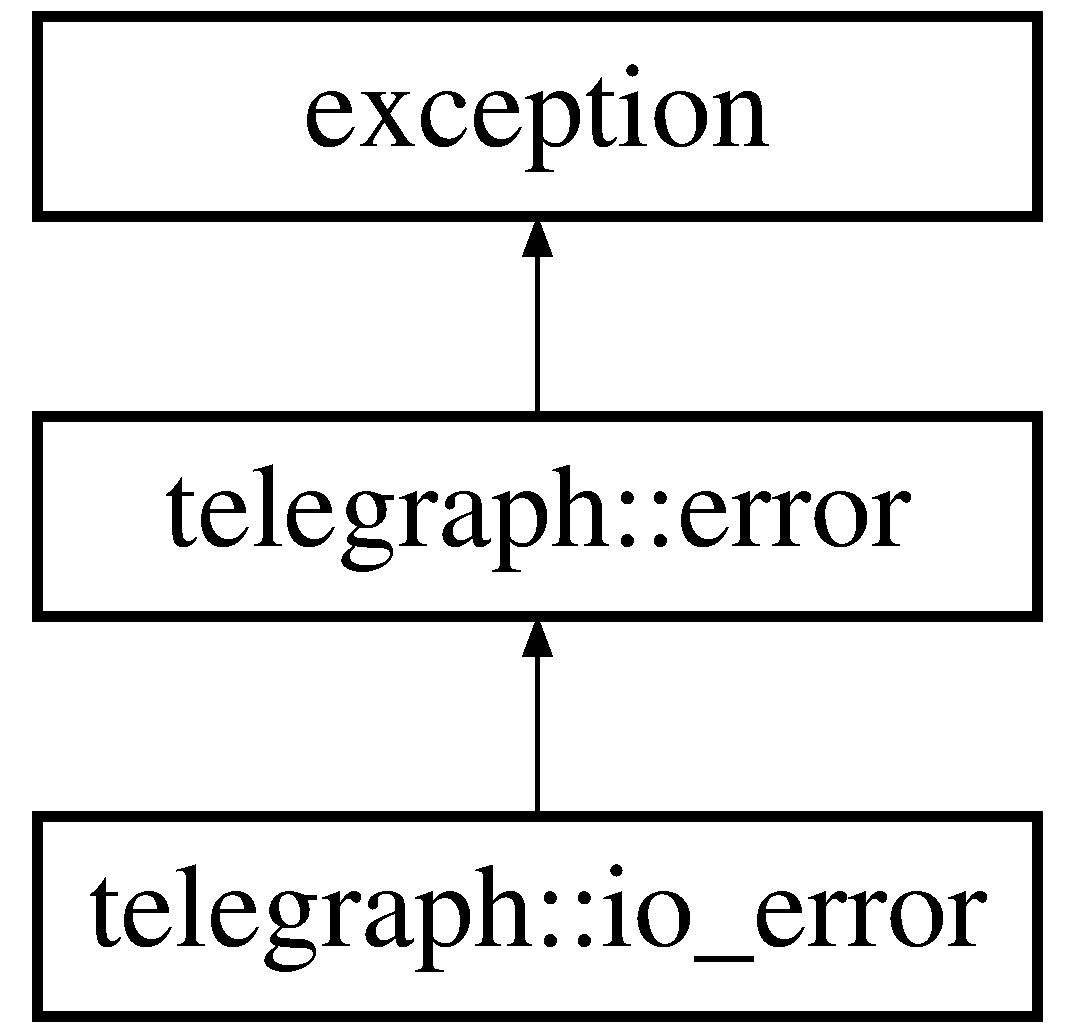
\includegraphics[height=3.000000cm]{classtelegraph_1_1io__error}
\end{center}
\end{figure}
\subsection*{Public Member Functions}
\begin{DoxyCompactItemize}
\item 
\hyperlink{classtelegraph_1_1io__error_a173bdfb9ed5c5ec6dd4d80a137834d41}{io\+\_\+error} (const std\+::string\+\_\+view \&m)
\end{DoxyCompactItemize}


\subsection{Constructor \& Destructor Documentation}
\mbox{\Hypertarget{classtelegraph_1_1io__error_a173bdfb9ed5c5ec6dd4d80a137834d41}\label{classtelegraph_1_1io__error_a173bdfb9ed5c5ec6dd4d80a137834d41}} 
\index{telegraph\+::io\+\_\+error@{telegraph\+::io\+\_\+error}!io\+\_\+error@{io\+\_\+error}}
\index{io\+\_\+error@{io\+\_\+error}!telegraph\+::io\+\_\+error@{telegraph\+::io\+\_\+error}}
\subsubsection{\texorpdfstring{io\+\_\+error()}{io\_error()}}
{\footnotesize\ttfamily telegraph\+::io\+\_\+error\+::io\+\_\+error (\begin{DoxyParamCaption}\item[{const std\+::string\+\_\+view \&}]{m }\end{DoxyParamCaption})\hspace{0.3cm}{\ttfamily [inline]}}



The documentation for this class was generated from the following file\+:\begin{DoxyCompactItemize}
\item 
\hyperlink{errors_8hpp}{errors.\+hpp}\end{DoxyCompactItemize}

\hypertarget{structstdext_1_1inplace__function__detail_1_1is__inplace__function}{}\section{stdext\+:\+:inplace\+\_\+function\+\_\+detail\+:\+:is\+\_\+inplace\+\_\+function$<$ class $>$ Struct Template Reference}
\label{structstdext_1_1inplace__function__detail_1_1is__inplace__function}\index{stdext\+::inplace\+\_\+function\+\_\+detail\+::is\+\_\+inplace\+\_\+function$<$ class $>$@{stdext\+::inplace\+\_\+function\+\_\+detail\+::is\+\_\+inplace\+\_\+function$<$ class $>$}}


{\ttfamily \#include $<$inplace\+\_\+function.\+hpp$>$}

Inheritance diagram for stdext\+:\+:inplace\+\_\+function\+\_\+detail\+:\+:is\+\_\+inplace\+\_\+function$<$ class $>$\+:\begin{figure}[H]
\begin{center}
\leavevmode
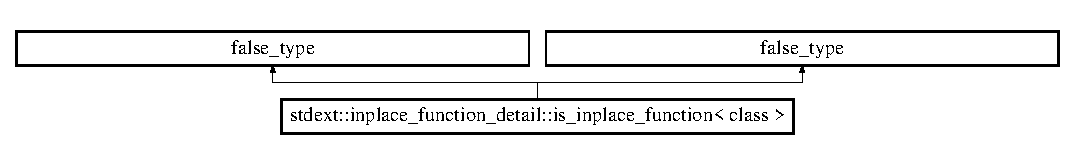
\includegraphics[height=1.573034cm]{structstdext_1_1inplace__function__detail_1_1is__inplace__function}
\end{center}
\end{figure}


The documentation for this struct was generated from the following file\+:\begin{DoxyCompactItemize}
\item 
\hyperlink{gen_2telegen_2inplace__function_8hpp}{gen/telegen/inplace\+\_\+function.\+hpp}\end{DoxyCompactItemize}

\hypertarget{structstdext_1_1inplace__function__detail_1_1is__inplace__function_3_01inplace__function_3_01Sig_00_01Cap_00_01Align_01_4_01_4}{}\section{stdext\+:\+:inplace\+\_\+function\+\_\+detail\+:\+:is\+\_\+inplace\+\_\+function$<$ inplace\+\_\+function$<$ Sig, Cap, Align $>$ $>$ Struct Template Reference}
\label{structstdext_1_1inplace__function__detail_1_1is__inplace__function_3_01inplace__function_3_01Sig_00_01Cap_00_01Align_01_4_01_4}\index{stdext\+::inplace\+\_\+function\+\_\+detail\+::is\+\_\+inplace\+\_\+function$<$ inplace\+\_\+function$<$ Sig, Cap, Align $>$ $>$@{stdext\+::inplace\+\_\+function\+\_\+detail\+::is\+\_\+inplace\+\_\+function$<$ inplace\+\_\+function$<$ Sig, Cap, Align $>$ $>$}}


{\ttfamily \#include $<$inplace\+\_\+function.\+hpp$>$}

Inheritance diagram for stdext\+:\+:inplace\+\_\+function\+\_\+detail\+:\+:is\+\_\+inplace\+\_\+function$<$ inplace\+\_\+function$<$ Sig, Cap, Align $>$ $>$\+:\begin{figure}[H]
\begin{center}
\leavevmode
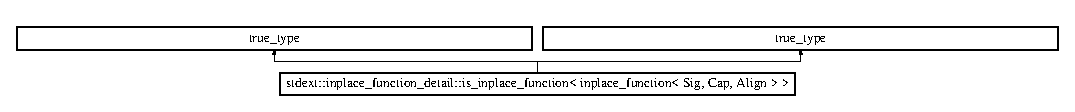
\includegraphics[height=1.052632cm]{structstdext_1_1inplace__function__detail_1_1is__inplace__function_3_01inplace__function_3_01Sig_00_01Cap_00_01Align_01_4_01_4}
\end{center}
\end{figure}


The documentation for this struct was generated from the following file\+:\begin{DoxyCompactItemize}
\item 
\hyperlink{gen_2telegen_2inplace__function_8hpp}{gen/telegen/inplace\+\_\+function.\+hpp}\end{DoxyCompactItemize}

\hypertarget{structstdext_1_1inplace__function__detail_1_1is__invocable__r__impl}{}\section{stdext\+:\+:inplace\+\_\+function\+\_\+detail\+:\+:is\+\_\+invocable\+\_\+r\+\_\+impl$<$ class, R, F, Args $>$ Struct Template Reference}
\label{structstdext_1_1inplace__function__detail_1_1is__invocable__r__impl}\index{stdext\+::inplace\+\_\+function\+\_\+detail\+::is\+\_\+invocable\+\_\+r\+\_\+impl$<$ class, R, F, Args $>$@{stdext\+::inplace\+\_\+function\+\_\+detail\+::is\+\_\+invocable\+\_\+r\+\_\+impl$<$ class, R, F, Args $>$}}


{\ttfamily \#include $<$inplace\+\_\+function.\+hpp$>$}

Inheritance diagram for stdext\+:\+:inplace\+\_\+function\+\_\+detail\+:\+:is\+\_\+invocable\+\_\+r\+\_\+impl$<$ class, R, F, Args $>$\+:\begin{figure}[H]
\begin{center}
\leavevmode
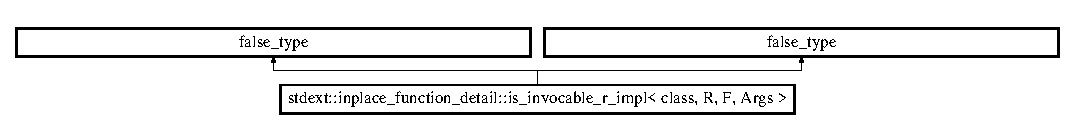
\includegraphics[height=1.305361cm]{structstdext_1_1inplace__function__detail_1_1is__invocable__r__impl}
\end{center}
\end{figure}


The documentation for this struct was generated from the following file\+:\begin{DoxyCompactItemize}
\item 
\hyperlink{gen_2telegen_2inplace__function_8hpp}{gen/telegen/inplace\+\_\+function.\+hpp}\end{DoxyCompactItemize}

\hypertarget{structstdext_1_1inplace__function__detail_1_1is__invocable__r__impl_3_01decltype_07accept_3_01R_32d81c51f4037807d0fe4b47c34d0755}{}\section{stdext\+:\+:inplace\+\_\+function\+\_\+detail\+:\+:is\+\_\+invocable\+\_\+r\+\_\+impl$<$ decltype(accept$<$ R $>$(std\+:\+:declval$<$ F $>$()(std\+:\+:declval$<$ Args $>$()...))), R, F, Args... $>$ Struct Template Reference}
\label{structstdext_1_1inplace__function__detail_1_1is__invocable__r__impl_3_01decltype_07accept_3_01R_32d81c51f4037807d0fe4b47c34d0755}\index{stdext\+::inplace\+\_\+function\+\_\+detail\+::is\+\_\+invocable\+\_\+r\+\_\+impl$<$ decltype(accept$<$ R $>$(std\+::declval$<$ F $>$()(std\+::declval$<$ Args $>$()...))), R, F, Args... $>$@{stdext\+::inplace\+\_\+function\+\_\+detail\+::is\+\_\+invocable\+\_\+r\+\_\+impl$<$ decltype(accept$<$ R $>$(std\+::declval$<$ F $>$()(std\+::declval$<$ Args $>$()...))), R, F, Args... $>$}}


{\ttfamily \#include $<$inplace\+\_\+function.\+hpp$>$}

Inheritance diagram for stdext\+:\+:inplace\+\_\+function\+\_\+detail\+:\+:is\+\_\+invocable\+\_\+r\+\_\+impl$<$ decltype(accept$<$ R $>$(std\+:\+:declval$<$ F $>$()(std\+:\+:declval$<$ Args $>$()...))), R, F, Args... $>$\+:\begin{figure}[H]
\begin{center}
\leavevmode
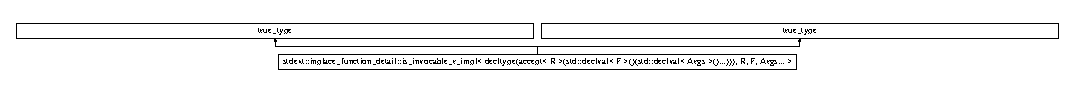
\includegraphics[height=0.707965cm]{structstdext_1_1inplace__function__detail_1_1is__invocable__r__impl_3_01decltype_07accept_3_01R_32d81c51f4037807d0fe4b47c34d0755}
\end{center}
\end{figure}


The documentation for this struct was generated from the following file\+:\begin{DoxyCompactItemize}
\item 
\hyperlink{gen_2telegen_2inplace__function_8hpp}{gen/telegen/inplace\+\_\+function.\+hpp}\end{DoxyCompactItemize}

\hypertarget{structstdext_1_1inplace__function__detail_1_1is__invocable__r__impl_3_01decltype_07std_1_1declva0b72e3b51b5a25ed55b63381e8d17b0a}{}\section{stdext\+:\+:inplace\+\_\+function\+\_\+detail\+:\+:is\+\_\+invocable\+\_\+r\+\_\+impl$<$ decltype(std\+:\+:declval$<$ F $>$()(std\+:\+:declval$<$ Args $>$()...), void()), const void, F, Args... $>$ Struct Template Reference}
\label{structstdext_1_1inplace__function__detail_1_1is__invocable__r__impl_3_01decltype_07std_1_1declva0b72e3b51b5a25ed55b63381e8d17b0a}\index{stdext\+::inplace\+\_\+function\+\_\+detail\+::is\+\_\+invocable\+\_\+r\+\_\+impl$<$ decltype(std\+::declval$<$ F $>$()(std\+::declval$<$ Args $>$()...), void()), const void, F, Args... $>$@{stdext\+::inplace\+\_\+function\+\_\+detail\+::is\+\_\+invocable\+\_\+r\+\_\+impl$<$ decltype(std\+::declval$<$ F $>$()(std\+::declval$<$ Args $>$()...), void()), const void, F, Args... $>$}}


{\ttfamily \#include $<$inplace\+\_\+function.\+hpp$>$}

Inheritance diagram for stdext\+:\+:inplace\+\_\+function\+\_\+detail\+:\+:is\+\_\+invocable\+\_\+r\+\_\+impl$<$ decltype(std\+:\+:declval$<$ F $>$()(std\+:\+:declval$<$ Args $>$()...), void()), const void, F, Args... $>$\+:\begin{figure}[H]
\begin{center}
\leavevmode
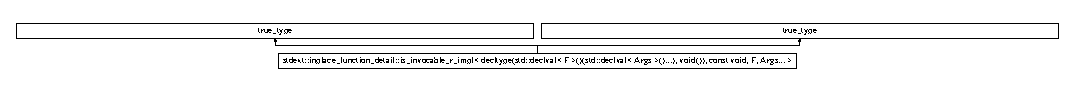
\includegraphics[height=0.695652cm]{structstdext_1_1inplace__function__detail_1_1is__invocable__r__impl_3_01decltype_07std_1_1declva0b72e3b51b5a25ed55b63381e8d17b0a}
\end{center}
\end{figure}


The documentation for this struct was generated from the following file\+:\begin{DoxyCompactItemize}
\item 
\hyperlink{gen_2telegen_2inplace__function_8hpp}{gen/telegen/inplace\+\_\+function.\+hpp}\end{DoxyCompactItemize}

\hypertarget{structstdext_1_1inplace__function__detail_1_1is__invocable__r__impl_3_01decltype_07std_1_1declva53be7366370c87c5d74810a4225ea3b9}{}\section{stdext\+:\+:inplace\+\_\+function\+\_\+detail\+:\+:is\+\_\+invocable\+\_\+r\+\_\+impl$<$ decltype(std\+:\+:declval$<$ F $>$()(std\+:\+:declval$<$ Args $>$()...), void()), void, F, Args... $>$ Struct Template Reference}
\label{structstdext_1_1inplace__function__detail_1_1is__invocable__r__impl_3_01decltype_07std_1_1declva53be7366370c87c5d74810a4225ea3b9}\index{stdext\+::inplace\+\_\+function\+\_\+detail\+::is\+\_\+invocable\+\_\+r\+\_\+impl$<$ decltype(std\+::declval$<$ F $>$()(std\+::declval$<$ Args $>$()...), void()), void, F, Args... $>$@{stdext\+::inplace\+\_\+function\+\_\+detail\+::is\+\_\+invocable\+\_\+r\+\_\+impl$<$ decltype(std\+::declval$<$ F $>$()(std\+::declval$<$ Args $>$()...), void()), void, F, Args... $>$}}


{\ttfamily \#include $<$inplace\+\_\+function.\+hpp$>$}

Inheritance diagram for stdext\+:\+:inplace\+\_\+function\+\_\+detail\+:\+:is\+\_\+invocable\+\_\+r\+\_\+impl$<$ decltype(std\+:\+:declval$<$ F $>$()(std\+:\+:declval$<$ Args $>$()...), void()), void, F, Args... $>$\+:\begin{figure}[H]
\begin{center}
\leavevmode
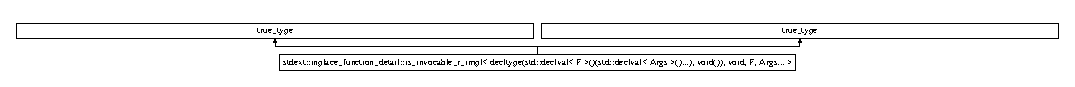
\includegraphics[height=0.727273cm]{structstdext_1_1inplace__function__detail_1_1is__invocable__r__impl_3_01decltype_07std_1_1declva53be7366370c87c5d74810a4225ea3b9}
\end{center}
\end{figure}


The documentation for this struct was generated from the following file\+:\begin{DoxyCompactItemize}
\item 
\hyperlink{gen_2telegen_2inplace__function_8hpp}{gen/telegen/inplace\+\_\+function.\+hpp}\end{DoxyCompactItemize}

\hypertarget{structstdext_1_1inplace__function__detail_1_1is__valid__inplace__dst}{}\section{stdext\+:\+:inplace\+\_\+function\+\_\+detail\+:\+:is\+\_\+valid\+\_\+inplace\+\_\+dst$<$ Dst\+Cap, Dst\+Align, Src\+Cap, Src\+Align $>$ Struct Template Reference}
\label{structstdext_1_1inplace__function__detail_1_1is__valid__inplace__dst}\index{stdext\+::inplace\+\_\+function\+\_\+detail\+::is\+\_\+valid\+\_\+inplace\+\_\+dst$<$ Dst\+Cap, Dst\+Align, Src\+Cap, Src\+Align $>$@{stdext\+::inplace\+\_\+function\+\_\+detail\+::is\+\_\+valid\+\_\+inplace\+\_\+dst$<$ Dst\+Cap, Dst\+Align, Src\+Cap, Src\+Align $>$}}


{\ttfamily \#include $<$inplace\+\_\+function.\+hpp$>$}

Inheritance diagram for stdext\+:\+:inplace\+\_\+function\+\_\+detail\+:\+:is\+\_\+valid\+\_\+inplace\+\_\+dst$<$ Dst\+Cap, Dst\+Align, Src\+Cap, Src\+Align $>$\+:\begin{figure}[H]
\begin{center}
\leavevmode
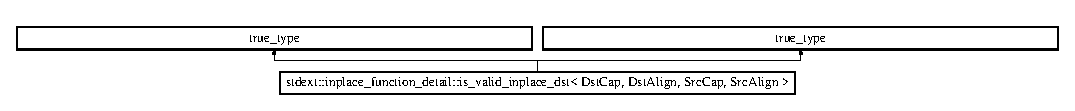
\includegraphics[height=1.038961cm]{structstdext_1_1inplace__function__detail_1_1is__valid__inplace__dst}
\end{center}
\end{figure}


The documentation for this struct was generated from the following file\+:\begin{DoxyCompactItemize}
\item 
\hyperlink{gen_2telegen_2inplace__function_8hpp}{gen/telegen/inplace\+\_\+function.\+hpp}\end{DoxyCompactItemize}

\hypertarget{classtelegraph_1_1json__parser}{}\section{telegraph\+:\+:json\+\_\+parser Class Reference}
\label{classtelegraph_1_1json__parser}\index{telegraph\+::json\+\_\+parser@{telegraph\+::json\+\_\+parser}}


{\ttfamily \#include $<$json.\+hpp$>$}

\subsection*{Public Member Functions}
\begin{DoxyCompactItemize}
\item 
\hyperlink{namespacetelegraph_ab87b47a6b955c365ddd74c343ecc16f4}{json} \hyperlink{classtelegraph_1_1json__parser_ad3f209cfb4e81aa7c1d5fb577b09de30}{parse\+\_\+file} (const std\+::string \&file)
\end{DoxyCompactItemize}


\subsection{Member Function Documentation}
\mbox{\Hypertarget{classtelegraph_1_1json__parser_ad3f209cfb4e81aa7c1d5fb577b09de30}\label{classtelegraph_1_1json__parser_ad3f209cfb4e81aa7c1d5fb577b09de30}} 
\index{telegraph\+::json\+\_\+parser@{telegraph\+::json\+\_\+parser}!parse\+\_\+file@{parse\+\_\+file}}
\index{parse\+\_\+file@{parse\+\_\+file}!telegraph\+::json\+\_\+parser@{telegraph\+::json\+\_\+parser}}
\subsubsection{\texorpdfstring{parse\+\_\+file()}{parse\_file()}}
{\footnotesize\ttfamily \hyperlink{namespacetelegraph_ab87b47a6b955c365ddd74c343ecc16f4}{json} telegraph\+::json\+\_\+parser\+::parse\+\_\+file (\begin{DoxyParamCaption}\item[{const std\+::string \&}]{file }\end{DoxyParamCaption})}



The documentation for this class was generated from the following files\+:\begin{DoxyCompactItemize}
\item 
\hyperlink{json_8hpp}{json.\+hpp}\item 
\hyperlink{json_8cpp}{json.\+cpp}\end{DoxyCompactItemize}

\hypertarget{classtelegraph_1_1local__component}{}\section{telegraph\+:\+:local\+\_\+component Class Reference}
\label{classtelegraph_1_1local__component}\index{telegraph\+::local\+\_\+component@{telegraph\+::local\+\_\+component}}


{\ttfamily \#include $<$namespace.\+hpp$>$}

Inheritance diagram for telegraph\+:\+:local\+\_\+component\+:\begin{figure}[H]
\begin{center}
\leavevmode
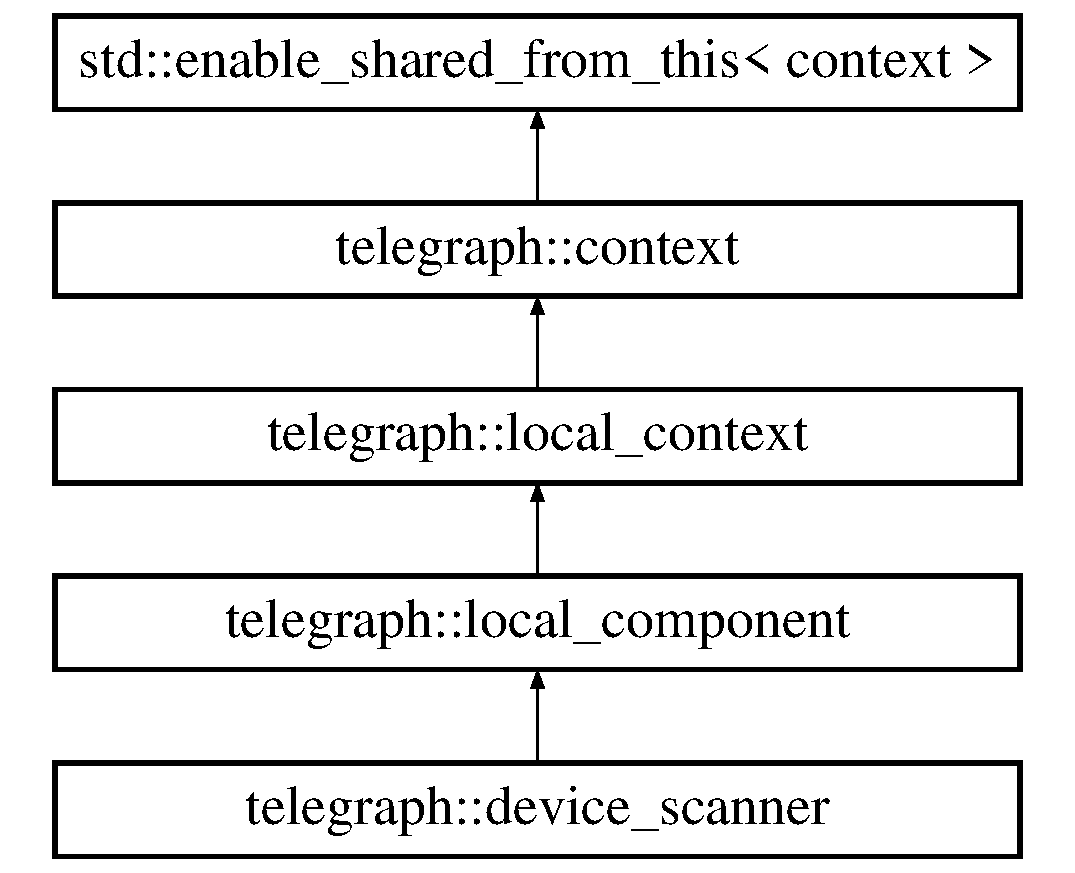
\includegraphics[height=5.000000cm]{classtelegraph_1_1local__component}
\end{center}
\end{figure}
\subsection*{Public Member Functions}
\begin{DoxyCompactItemize}
\item 
\hyperlink{classtelegraph_1_1local__component_a4cd9cd1728ba53391553b81dbb4e3494}{local\+\_\+component} (io\+::io\+\_\+context \&ioc, const std\+::string\+\_\+view \&name, const std\+::string\+\_\+view \&type, const \hyperlink{classtelegraph_1_1params}{params} \&i)
\item 
std\+::shared\+\_\+ptr$<$ \hyperlink{classtelegraph_1_1node}{node} $>$ \hyperlink{classtelegraph_1_1local__component_abbeb3b12dc95e19e1a2972e9a374fd33}{fetch} (\hyperlink{structboost_1_1asio_1_1yield__ctx}{io\+::yield\+\_\+ctx} \&ctx) override
\item 
\hyperlink{namespacetelegraph_a58641aa5b1a2cbdb0431916a87069f64}{subscription\+\_\+ptr} \hyperlink{classtelegraph_1_1local__component_a53aa0199bd938578a6400cfd3a19c86f}{subscribe} (\hyperlink{structboost_1_1asio_1_1yield__ctx}{io\+::yield\+\_\+ctx} \&ctx, const std\+::vector$<$ std\+::string\+\_\+view $>$ \&\hyperlink{classtelegraph_1_1variable}{variable}, float min\+\_\+interval, float max\+\_\+interval, float timeout) override
\item 
\hyperlink{namespacetelegraph_a58641aa5b1a2cbdb0431916a87069f64}{subscription\+\_\+ptr} \hyperlink{classtelegraph_1_1local__component_a5a2282f1cf80dce32ed26e37c956d5c4}{subscribe} (\hyperlink{structboost_1_1asio_1_1yield__ctx}{io\+::yield\+\_\+ctx} \&ctx, const \hyperlink{classtelegraph_1_1variable}{variable} $\ast$v, float min\+\_\+interval, float max\+\_\+interval, float timeout) override
\item 
\hyperlink{classtelegraph_1_1value}{value} \hyperlink{classtelegraph_1_1local__component_af4d74d161754055d3f811bfe95a59f26}{call} (\hyperlink{structboost_1_1asio_1_1yield__ctx}{io\+::yield\+\_\+ctx} \&ctx, \hyperlink{classtelegraph_1_1action}{action} $\ast$a, \hyperlink{classtelegraph_1_1value}{value} v, float timeout) override
\item 
\hyperlink{classtelegraph_1_1value}{value} \hyperlink{classtelegraph_1_1local__component_a6fa6fbf49a0d77a8da54b4a77b578edd}{call} (\hyperlink{structboost_1_1asio_1_1yield__ctx}{io\+::yield\+\_\+ctx} \&ctx, const std\+::vector$<$ std\+::string\+\_\+view $>$ \&a, \hyperlink{classtelegraph_1_1value}{value} v, float timeout) override
\item 
bool \hyperlink{classtelegraph_1_1local__component_ac546cfea4802ef3ca125c5dc183adf6c}{write\+\_\+data} (\hyperlink{structboost_1_1asio_1_1yield__ctx}{io\+::yield\+\_\+ctx} \&yield, \hyperlink{classtelegraph_1_1variable}{variable} $\ast$v, const std\+::vector$<$ \hyperlink{classtelegraph_1_1data__point}{data\+\_\+point} $>$ \&data) override
\item 
bool \hyperlink{classtelegraph_1_1local__component_a572a4116130a4b7ad270701eba2af0e7}{write\+\_\+data} (\hyperlink{structboost_1_1asio_1_1yield__ctx}{io\+::yield\+\_\+ctx} \&yield, const std\+::vector$<$ std\+::string\+\_\+view $>$ \&var, const std\+::vector$<$ \hyperlink{classtelegraph_1_1data__point}{data\+\_\+point} $>$ \&data) override
\item 
\hyperlink{namespacetelegraph_a6ffe775ac48dca2a4013b53d692199c8}{data\+\_\+query\+\_\+ptr} \hyperlink{classtelegraph_1_1local__component_a4410ca44a41de1c139273efd31f281c4}{query\+\_\+data} (\hyperlink{structboost_1_1asio_1_1yield__ctx}{io\+::yield\+\_\+ctx} \&yield, const \hyperlink{classtelegraph_1_1variable}{variable} $\ast$v) override
\item 
\hyperlink{namespacetelegraph_a6ffe775ac48dca2a4013b53d692199c8}{data\+\_\+query\+\_\+ptr} \hyperlink{classtelegraph_1_1local__component_ad8c3abb4f9e6ab31b0590beac901eec5}{query\+\_\+data} (\hyperlink{structboost_1_1asio_1_1yield__ctx}{io\+::yield\+\_\+ctx} \&yield, const std\+::vector$<$ std\+::string\+\_\+view $>$ \&v) override
\end{DoxyCompactItemize}
\subsection*{Additional Inherited Members}


\subsection{Constructor \& Destructor Documentation}
\mbox{\Hypertarget{classtelegraph_1_1local__component_a4cd9cd1728ba53391553b81dbb4e3494}\label{classtelegraph_1_1local__component_a4cd9cd1728ba53391553b81dbb4e3494}} 
\index{telegraph\+::local\+\_\+component@{telegraph\+::local\+\_\+component}!local\+\_\+component@{local\+\_\+component}}
\index{local\+\_\+component@{local\+\_\+component}!telegraph\+::local\+\_\+component@{telegraph\+::local\+\_\+component}}
\subsubsection{\texorpdfstring{local\+\_\+component()}{local\_component()}}
{\footnotesize\ttfamily telegraph\+::local\+\_\+component\+::local\+\_\+component (\begin{DoxyParamCaption}\item[{io\+::io\+\_\+context \&}]{ioc,  }\item[{const std\+::string\+\_\+view \&}]{name,  }\item[{const std\+::string\+\_\+view \&}]{type,  }\item[{const \hyperlink{classtelegraph_1_1params}{params} \&}]{i }\end{DoxyParamCaption})}



\subsection{Member Function Documentation}
\mbox{\Hypertarget{classtelegraph_1_1local__component_af4d74d161754055d3f811bfe95a59f26}\label{classtelegraph_1_1local__component_af4d74d161754055d3f811bfe95a59f26}} 
\index{telegraph\+::local\+\_\+component@{telegraph\+::local\+\_\+component}!call@{call}}
\index{call@{call}!telegraph\+::local\+\_\+component@{telegraph\+::local\+\_\+component}}
\subsubsection{\texorpdfstring{call()}{call()}\hspace{0.1cm}{\footnotesize\ttfamily [1/2]}}
{\footnotesize\ttfamily \hyperlink{classtelegraph_1_1value}{value} telegraph\+::local\+\_\+component\+::call (\begin{DoxyParamCaption}\item[{\hyperlink{structboost_1_1asio_1_1yield__ctx}{io\+::yield\+\_\+ctx} \&}]{ctx,  }\item[{\hyperlink{classtelegraph_1_1action}{action} $\ast$}]{a,  }\item[{\hyperlink{classtelegraph_1_1value}{value}}]{v,  }\item[{float}]{timeout }\end{DoxyParamCaption})\hspace{0.3cm}{\ttfamily [inline]}, {\ttfamily [override]}, {\ttfamily [virtual]}}



Implements \hyperlink{classtelegraph_1_1context_a72da471eb635e5505b10d2f1103359ac}{telegraph\+::context}.

\mbox{\Hypertarget{classtelegraph_1_1local__component_a6fa6fbf49a0d77a8da54b4a77b578edd}\label{classtelegraph_1_1local__component_a6fa6fbf49a0d77a8da54b4a77b578edd}} 
\index{telegraph\+::local\+\_\+component@{telegraph\+::local\+\_\+component}!call@{call}}
\index{call@{call}!telegraph\+::local\+\_\+component@{telegraph\+::local\+\_\+component}}
\subsubsection{\texorpdfstring{call()}{call()}\hspace{0.1cm}{\footnotesize\ttfamily [2/2]}}
{\footnotesize\ttfamily \hyperlink{classtelegraph_1_1value}{value} telegraph\+::local\+\_\+component\+::call (\begin{DoxyParamCaption}\item[{\hyperlink{structboost_1_1asio_1_1yield__ctx}{io\+::yield\+\_\+ctx} \&}]{ctx,  }\item[{const std\+::vector$<$ std\+::string\+\_\+view $>$ \&}]{a,  }\item[{\hyperlink{classtelegraph_1_1value}{value}}]{v,  }\item[{float}]{timeout }\end{DoxyParamCaption})\hspace{0.3cm}{\ttfamily [inline]}, {\ttfamily [override]}, {\ttfamily [virtual]}}



Implements \hyperlink{classtelegraph_1_1context_a0798d49ea0874a870d4c980f6f09b6c2}{telegraph\+::context}.

\mbox{\Hypertarget{classtelegraph_1_1local__component_abbeb3b12dc95e19e1a2972e9a374fd33}\label{classtelegraph_1_1local__component_abbeb3b12dc95e19e1a2972e9a374fd33}} 
\index{telegraph\+::local\+\_\+component@{telegraph\+::local\+\_\+component}!fetch@{fetch}}
\index{fetch@{fetch}!telegraph\+::local\+\_\+component@{telegraph\+::local\+\_\+component}}
\subsubsection{\texorpdfstring{fetch()}{fetch()}}
{\footnotesize\ttfamily std\+::shared\+\_\+ptr$<$\hyperlink{classtelegraph_1_1node}{node}$>$ telegraph\+::local\+\_\+component\+::fetch (\begin{DoxyParamCaption}\item[{\hyperlink{structboost_1_1asio_1_1yield__ctx}{io\+::yield\+\_\+ctx} \&}]{ctx }\end{DoxyParamCaption})\hspace{0.3cm}{\ttfamily [inline]}, {\ttfamily [override]}, {\ttfamily [virtual]}}



Reimplemented from \hyperlink{classtelegraph_1_1local__context_aefadafdf25e6f6ba23c4b332872836e2}{telegraph\+::local\+\_\+context}.

\mbox{\Hypertarget{classtelegraph_1_1local__component_a4410ca44a41de1c139273efd31f281c4}\label{classtelegraph_1_1local__component_a4410ca44a41de1c139273efd31f281c4}} 
\index{telegraph\+::local\+\_\+component@{telegraph\+::local\+\_\+component}!query\+\_\+data@{query\+\_\+data}}
\index{query\+\_\+data@{query\+\_\+data}!telegraph\+::local\+\_\+component@{telegraph\+::local\+\_\+component}}
\subsubsection{\texorpdfstring{query\+\_\+data()}{query\_data()}\hspace{0.1cm}{\footnotesize\ttfamily [1/2]}}
{\footnotesize\ttfamily \hyperlink{namespacetelegraph_a6ffe775ac48dca2a4013b53d692199c8}{data\+\_\+query\+\_\+ptr} telegraph\+::local\+\_\+component\+::query\+\_\+data (\begin{DoxyParamCaption}\item[{\hyperlink{structboost_1_1asio_1_1yield__ctx}{io\+::yield\+\_\+ctx} \&}]{yield,  }\item[{const \hyperlink{classtelegraph_1_1variable}{variable} $\ast$}]{v }\end{DoxyParamCaption})\hspace{0.3cm}{\ttfamily [inline]}, {\ttfamily [override]}, {\ttfamily [virtual]}}



Implements \hyperlink{classtelegraph_1_1context_a301114c9b73194507ae58221566a3e57}{telegraph\+::context}.

\mbox{\Hypertarget{classtelegraph_1_1local__component_ad8c3abb4f9e6ab31b0590beac901eec5}\label{classtelegraph_1_1local__component_ad8c3abb4f9e6ab31b0590beac901eec5}} 
\index{telegraph\+::local\+\_\+component@{telegraph\+::local\+\_\+component}!query\+\_\+data@{query\+\_\+data}}
\index{query\+\_\+data@{query\+\_\+data}!telegraph\+::local\+\_\+component@{telegraph\+::local\+\_\+component}}
\subsubsection{\texorpdfstring{query\+\_\+data()}{query\_data()}\hspace{0.1cm}{\footnotesize\ttfamily [2/2]}}
{\footnotesize\ttfamily \hyperlink{namespacetelegraph_a6ffe775ac48dca2a4013b53d692199c8}{data\+\_\+query\+\_\+ptr} telegraph\+::local\+\_\+component\+::query\+\_\+data (\begin{DoxyParamCaption}\item[{\hyperlink{structboost_1_1asio_1_1yield__ctx}{io\+::yield\+\_\+ctx} \&}]{yield,  }\item[{const std\+::vector$<$ std\+::string\+\_\+view $>$ \&}]{v }\end{DoxyParamCaption})\hspace{0.3cm}{\ttfamily [inline]}, {\ttfamily [override]}, {\ttfamily [virtual]}}



Implements \hyperlink{classtelegraph_1_1context_a34793623d2a2def580ad0b8710c74c6d}{telegraph\+::context}.

\mbox{\Hypertarget{classtelegraph_1_1local__component_a53aa0199bd938578a6400cfd3a19c86f}\label{classtelegraph_1_1local__component_a53aa0199bd938578a6400cfd3a19c86f}} 
\index{telegraph\+::local\+\_\+component@{telegraph\+::local\+\_\+component}!subscribe@{subscribe}}
\index{subscribe@{subscribe}!telegraph\+::local\+\_\+component@{telegraph\+::local\+\_\+component}}
\subsubsection{\texorpdfstring{subscribe()}{subscribe()}\hspace{0.1cm}{\footnotesize\ttfamily [1/2]}}
{\footnotesize\ttfamily \hyperlink{namespacetelegraph_a58641aa5b1a2cbdb0431916a87069f64}{subscription\+\_\+ptr} telegraph\+::local\+\_\+component\+::subscribe (\begin{DoxyParamCaption}\item[{\hyperlink{structboost_1_1asio_1_1yield__ctx}{io\+::yield\+\_\+ctx} \&}]{ctx,  }\item[{const std\+::vector$<$ std\+::string\+\_\+view $>$ \&}]{variable,  }\item[{float}]{min\+\_\+interval,  }\item[{float}]{max\+\_\+interval,  }\item[{float}]{timeout }\end{DoxyParamCaption})\hspace{0.3cm}{\ttfamily [inline]}, {\ttfamily [override]}, {\ttfamily [virtual]}}



Implements \hyperlink{classtelegraph_1_1context_a8db167973f187f707a4108e112683969}{telegraph\+::context}.

\mbox{\Hypertarget{classtelegraph_1_1local__component_a5a2282f1cf80dce32ed26e37c956d5c4}\label{classtelegraph_1_1local__component_a5a2282f1cf80dce32ed26e37c956d5c4}} 
\index{telegraph\+::local\+\_\+component@{telegraph\+::local\+\_\+component}!subscribe@{subscribe}}
\index{subscribe@{subscribe}!telegraph\+::local\+\_\+component@{telegraph\+::local\+\_\+component}}
\subsubsection{\texorpdfstring{subscribe()}{subscribe()}\hspace{0.1cm}{\footnotesize\ttfamily [2/2]}}
{\footnotesize\ttfamily \hyperlink{namespacetelegraph_a58641aa5b1a2cbdb0431916a87069f64}{subscription\+\_\+ptr} telegraph\+::local\+\_\+component\+::subscribe (\begin{DoxyParamCaption}\item[{\hyperlink{structboost_1_1asio_1_1yield__ctx}{io\+::yield\+\_\+ctx} \&}]{ctx,  }\item[{const \hyperlink{classtelegraph_1_1variable}{variable} $\ast$}]{v,  }\item[{float}]{min\+\_\+interval,  }\item[{float}]{max\+\_\+interval,  }\item[{float}]{timeout }\end{DoxyParamCaption})\hspace{0.3cm}{\ttfamily [inline]}, {\ttfamily [override]}, {\ttfamily [virtual]}}



Implements \hyperlink{classtelegraph_1_1context_aec3b3b0d7210a86f2ea2f5067ef8e922}{telegraph\+::context}.

\mbox{\Hypertarget{classtelegraph_1_1local__component_ac546cfea4802ef3ca125c5dc183adf6c}\label{classtelegraph_1_1local__component_ac546cfea4802ef3ca125c5dc183adf6c}} 
\index{telegraph\+::local\+\_\+component@{telegraph\+::local\+\_\+component}!write\+\_\+data@{write\+\_\+data}}
\index{write\+\_\+data@{write\+\_\+data}!telegraph\+::local\+\_\+component@{telegraph\+::local\+\_\+component}}
\subsubsection{\texorpdfstring{write\+\_\+data()}{write\_data()}\hspace{0.1cm}{\footnotesize\ttfamily [1/2]}}
{\footnotesize\ttfamily bool telegraph\+::local\+\_\+component\+::write\+\_\+data (\begin{DoxyParamCaption}\item[{\hyperlink{structboost_1_1asio_1_1yield__ctx}{io\+::yield\+\_\+ctx} \&}]{yield,  }\item[{\hyperlink{classtelegraph_1_1variable}{variable} $\ast$}]{v,  }\item[{const std\+::vector$<$ \hyperlink{classtelegraph_1_1data__point}{data\+\_\+point} $>$ \&}]{data }\end{DoxyParamCaption})\hspace{0.3cm}{\ttfamily [inline]}, {\ttfamily [override]}, {\ttfamily [virtual]}}



Implements \hyperlink{classtelegraph_1_1context_a6067b9a6f2590733c81f6a3b2ed9cba7}{telegraph\+::context}.

\mbox{\Hypertarget{classtelegraph_1_1local__component_a572a4116130a4b7ad270701eba2af0e7}\label{classtelegraph_1_1local__component_a572a4116130a4b7ad270701eba2af0e7}} 
\index{telegraph\+::local\+\_\+component@{telegraph\+::local\+\_\+component}!write\+\_\+data@{write\+\_\+data}}
\index{write\+\_\+data@{write\+\_\+data}!telegraph\+::local\+\_\+component@{telegraph\+::local\+\_\+component}}
\subsubsection{\texorpdfstring{write\+\_\+data()}{write\_data()}\hspace{0.1cm}{\footnotesize\ttfamily [2/2]}}
{\footnotesize\ttfamily bool telegraph\+::local\+\_\+component\+::write\+\_\+data (\begin{DoxyParamCaption}\item[{\hyperlink{structboost_1_1asio_1_1yield__ctx}{io\+::yield\+\_\+ctx} \&}]{yield,  }\item[{const std\+::vector$<$ std\+::string\+\_\+view $>$ \&}]{var,  }\item[{const std\+::vector$<$ \hyperlink{classtelegraph_1_1data__point}{data\+\_\+point} $>$ \&}]{data }\end{DoxyParamCaption})\hspace{0.3cm}{\ttfamily [inline]}, {\ttfamily [override]}, {\ttfamily [virtual]}}



Implements \hyperlink{classtelegraph_1_1context_a1f600d6159df21dd2750b1c706ca3412}{telegraph\+::context}.



The documentation for this class was generated from the following files\+:\begin{DoxyCompactItemize}
\item 
\hyperlink{local_2namespace_8hpp}{local/namespace.\+hpp}\item 
\hyperlink{namespace_8cpp}{namespace.\+cpp}\end{DoxyCompactItemize}

\hypertarget{classtelegraph_1_1local__context}{}\section{telegraph\+:\+:local\+\_\+context Class Reference}
\label{classtelegraph_1_1local__context}\index{telegraph\+::local\+\_\+context@{telegraph\+::local\+\_\+context}}


{\ttfamily \#include $<$namespace.\+hpp$>$}

Inheritance diagram for telegraph\+:\+:local\+\_\+context\+:\begin{figure}[H]
\begin{center}
\leavevmode
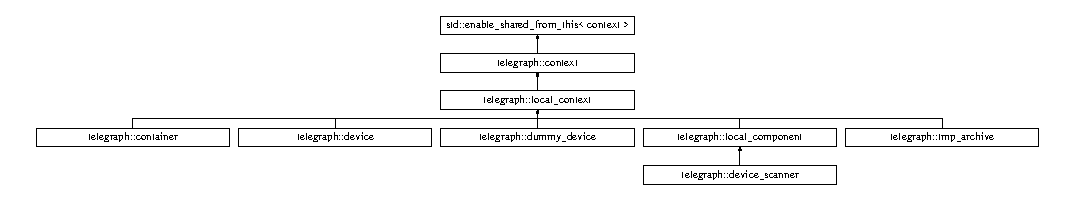
\includegraphics[height=2.258065cm]{classtelegraph_1_1local__context}
\end{center}
\end{figure}
\subsection*{Public Member Functions}
\begin{DoxyCompactItemize}
\item 
\hyperlink{classtelegraph_1_1local__context_a2f6fe87993dd07754131c5248c98c11d}{local\+\_\+context} (io\+::io\+\_\+context \&ioc, const std\+::string\+\_\+view \&name, const std\+::string\+\_\+view \&type, const \hyperlink{classtelegraph_1_1params}{params} \&i, const std\+::shared\+\_\+ptr$<$ \hyperlink{classtelegraph_1_1node}{node} $>$ \&tree, bool headless=false)
\item 
std\+::shared\+\_\+ptr$<$ \hyperlink{classtelegraph_1_1namespace__}{namespace\+\_\+} $>$ \hyperlink{classtelegraph_1_1local__context_a71a19090a93c3193615e61940fba918a}{get\+\_\+namespace} () override
\item 
std\+::shared\+\_\+ptr$<$ const \hyperlink{classtelegraph_1_1namespace__}{namespace\+\_\+} $>$ \hyperlink{classtelegraph_1_1local__context_aba1ff115df4b54bae75ea41580ba32b5}{get\+\_\+namespace} () const override
\item 
void \hyperlink{classtelegraph_1_1local__context_ab64632b088982a5f994708db99690f4f}{reg} (\hyperlink{structboost_1_1asio_1_1yield__ctx}{io\+::yield\+\_\+ctx} \&yield, const std\+::shared\+\_\+ptr$<$ \hyperlink{classtelegraph_1_1local__namespace}{local\+\_\+namespace} $>$ \&ns)
\item 
void \hyperlink{classtelegraph_1_1local__context_a301da16810636030a5098e4838587a99}{destroy} (\hyperlink{structboost_1_1asio_1_1yield__ctx}{io\+::yield\+\_\+ctx} \&yield) override
\item 
std\+::shared\+\_\+ptr$<$ \hyperlink{classtelegraph_1_1node}{node} $>$ \hyperlink{classtelegraph_1_1local__context_aefadafdf25e6f6ba23c4b332872836e2}{fetch} (\hyperlink{structboost_1_1asio_1_1yield__ctx}{io\+::yield\+\_\+ctx} \&) override
\end{DoxyCompactItemize}
\subsection*{Protected Attributes}
\begin{DoxyCompactItemize}
\item 
std\+::shared\+\_\+ptr$<$ \hyperlink{classtelegraph_1_1node}{node} $>$ \hyperlink{classtelegraph_1_1local__context_a16ab8680bd633b8b8554960bb8c48498}{tree\+\_\+}
\item 
std\+::weak\+\_\+ptr$<$ \hyperlink{classtelegraph_1_1local__namespace}{local\+\_\+namespace} $>$ \hyperlink{classtelegraph_1_1local__context_a4ad057dd5bede6236b3af44a18577831}{ns\+\_\+}
\end{DoxyCompactItemize}
\subsection*{Additional Inherited Members}


\subsection{Constructor \& Destructor Documentation}
\mbox{\Hypertarget{classtelegraph_1_1local__context_a2f6fe87993dd07754131c5248c98c11d}\label{classtelegraph_1_1local__context_a2f6fe87993dd07754131c5248c98c11d}} 
\index{telegraph\+::local\+\_\+context@{telegraph\+::local\+\_\+context}!local\+\_\+context@{local\+\_\+context}}
\index{local\+\_\+context@{local\+\_\+context}!telegraph\+::local\+\_\+context@{telegraph\+::local\+\_\+context}}
\subsubsection{\texorpdfstring{local\+\_\+context()}{local\_context()}}
{\footnotesize\ttfamily telegraph\+::local\+\_\+context\+::local\+\_\+context (\begin{DoxyParamCaption}\item[{io\+::io\+\_\+context \&}]{ioc,  }\item[{const std\+::string\+\_\+view \&}]{name,  }\item[{const std\+::string\+\_\+view \&}]{type,  }\item[{const \hyperlink{classtelegraph_1_1params}{params} \&}]{i,  }\item[{const std\+::shared\+\_\+ptr$<$ \hyperlink{classtelegraph_1_1node}{node} $>$ \&}]{tree,  }\item[{bool}]{headless = {\ttfamily false} }\end{DoxyParamCaption})}



\subsection{Member Function Documentation}
\mbox{\Hypertarget{classtelegraph_1_1local__context_a301da16810636030a5098e4838587a99}\label{classtelegraph_1_1local__context_a301da16810636030a5098e4838587a99}} 
\index{telegraph\+::local\+\_\+context@{telegraph\+::local\+\_\+context}!destroy@{destroy}}
\index{destroy@{destroy}!telegraph\+::local\+\_\+context@{telegraph\+::local\+\_\+context}}
\subsubsection{\texorpdfstring{destroy()}{destroy()}}
{\footnotesize\ttfamily void telegraph\+::local\+\_\+context\+::destroy (\begin{DoxyParamCaption}\item[{\hyperlink{structboost_1_1asio_1_1yield__ctx}{io\+::yield\+\_\+ctx} \&}]{yield }\end{DoxyParamCaption})\hspace{0.3cm}{\ttfamily [override]}, {\ttfamily [virtual]}}



Implements \hyperlink{classtelegraph_1_1context_a4017c1bcd9c84170a5cb612ae45d6fb4}{telegraph\+::context}.

\mbox{\Hypertarget{classtelegraph_1_1local__context_aefadafdf25e6f6ba23c4b332872836e2}\label{classtelegraph_1_1local__context_aefadafdf25e6f6ba23c4b332872836e2}} 
\index{telegraph\+::local\+\_\+context@{telegraph\+::local\+\_\+context}!fetch@{fetch}}
\index{fetch@{fetch}!telegraph\+::local\+\_\+context@{telegraph\+::local\+\_\+context}}
\subsubsection{\texorpdfstring{fetch()}{fetch()}}
{\footnotesize\ttfamily std\+::shared\+\_\+ptr$<$\hyperlink{classtelegraph_1_1node}{node}$>$ telegraph\+::local\+\_\+context\+::fetch (\begin{DoxyParamCaption}\item[{\hyperlink{structboost_1_1asio_1_1yield__ctx}{io\+::yield\+\_\+ctx} \&}]{ }\end{DoxyParamCaption})\hspace{0.3cm}{\ttfamily [inline]}, {\ttfamily [override]}, {\ttfamily [virtual]}}



Implements \hyperlink{classtelegraph_1_1context_aa2c0321629f2d51c8bc5632e418b305f}{telegraph\+::context}.



Reimplemented in \hyperlink{classtelegraph_1_1local__component_abbeb3b12dc95e19e1a2972e9a374fd33}{telegraph\+::local\+\_\+component}.

\mbox{\Hypertarget{classtelegraph_1_1local__context_a71a19090a93c3193615e61940fba918a}\label{classtelegraph_1_1local__context_a71a19090a93c3193615e61940fba918a}} 
\index{telegraph\+::local\+\_\+context@{telegraph\+::local\+\_\+context}!get\+\_\+namespace@{get\+\_\+namespace}}
\index{get\+\_\+namespace@{get\+\_\+namespace}!telegraph\+::local\+\_\+context@{telegraph\+::local\+\_\+context}}
\subsubsection{\texorpdfstring{get\+\_\+namespace()}{get\_namespace()}\hspace{0.1cm}{\footnotesize\ttfamily [1/2]}}
{\footnotesize\ttfamily std\+::shared\+\_\+ptr$<$\hyperlink{classtelegraph_1_1namespace__}{namespace\+\_\+}$>$ telegraph\+::local\+\_\+context\+::get\+\_\+namespace (\begin{DoxyParamCaption}{ }\end{DoxyParamCaption})\hspace{0.3cm}{\ttfamily [inline]}, {\ttfamily [override]}, {\ttfamily [virtual]}}



Implements \hyperlink{classtelegraph_1_1context_a84d92cca54be9c4e885e2673480e45a1}{telegraph\+::context}.

\mbox{\Hypertarget{classtelegraph_1_1local__context_aba1ff115df4b54bae75ea41580ba32b5}\label{classtelegraph_1_1local__context_aba1ff115df4b54bae75ea41580ba32b5}} 
\index{telegraph\+::local\+\_\+context@{telegraph\+::local\+\_\+context}!get\+\_\+namespace@{get\+\_\+namespace}}
\index{get\+\_\+namespace@{get\+\_\+namespace}!telegraph\+::local\+\_\+context@{telegraph\+::local\+\_\+context}}
\subsubsection{\texorpdfstring{get\+\_\+namespace()}{get\_namespace()}\hspace{0.1cm}{\footnotesize\ttfamily [2/2]}}
{\footnotesize\ttfamily std\+::shared\+\_\+ptr$<$const \hyperlink{classtelegraph_1_1namespace__}{namespace\+\_\+}$>$ telegraph\+::local\+\_\+context\+::get\+\_\+namespace (\begin{DoxyParamCaption}{ }\end{DoxyParamCaption}) const\hspace{0.3cm}{\ttfamily [inline]}, {\ttfamily [override]}, {\ttfamily [virtual]}}



Implements \hyperlink{classtelegraph_1_1context_a2f6c9ecc15cee66415828df9efa834a2}{telegraph\+::context}.

\mbox{\Hypertarget{classtelegraph_1_1local__context_ab64632b088982a5f994708db99690f4f}\label{classtelegraph_1_1local__context_ab64632b088982a5f994708db99690f4f}} 
\index{telegraph\+::local\+\_\+context@{telegraph\+::local\+\_\+context}!reg@{reg}}
\index{reg@{reg}!telegraph\+::local\+\_\+context@{telegraph\+::local\+\_\+context}}
\subsubsection{\texorpdfstring{reg()}{reg()}}
{\footnotesize\ttfamily void telegraph\+::local\+\_\+context\+::reg (\begin{DoxyParamCaption}\item[{\hyperlink{structboost_1_1asio_1_1yield__ctx}{io\+::yield\+\_\+ctx} \&}]{yield,  }\item[{const std\+::shared\+\_\+ptr$<$ \hyperlink{classtelegraph_1_1local__namespace}{local\+\_\+namespace} $>$ \&}]{ns }\end{DoxyParamCaption})}



\subsection{Member Data Documentation}
\mbox{\Hypertarget{classtelegraph_1_1local__context_a4ad057dd5bede6236b3af44a18577831}\label{classtelegraph_1_1local__context_a4ad057dd5bede6236b3af44a18577831}} 
\index{telegraph\+::local\+\_\+context@{telegraph\+::local\+\_\+context}!ns\+\_\+@{ns\+\_\+}}
\index{ns\+\_\+@{ns\+\_\+}!telegraph\+::local\+\_\+context@{telegraph\+::local\+\_\+context}}
\subsubsection{\texorpdfstring{ns\+\_\+}{ns\_}}
{\footnotesize\ttfamily std\+::weak\+\_\+ptr$<$\hyperlink{classtelegraph_1_1local__namespace}{local\+\_\+namespace}$>$ telegraph\+::local\+\_\+context\+::ns\+\_\+\hspace{0.3cm}{\ttfamily [protected]}}

\mbox{\Hypertarget{classtelegraph_1_1local__context_a16ab8680bd633b8b8554960bb8c48498}\label{classtelegraph_1_1local__context_a16ab8680bd633b8b8554960bb8c48498}} 
\index{telegraph\+::local\+\_\+context@{telegraph\+::local\+\_\+context}!tree\+\_\+@{tree\+\_\+}}
\index{tree\+\_\+@{tree\+\_\+}!telegraph\+::local\+\_\+context@{telegraph\+::local\+\_\+context}}
\subsubsection{\texorpdfstring{tree\+\_\+}{tree\_}}
{\footnotesize\ttfamily std\+::shared\+\_\+ptr$<$\hyperlink{classtelegraph_1_1node}{node}$>$ telegraph\+::local\+\_\+context\+::tree\+\_\+\hspace{0.3cm}{\ttfamily [protected]}}



The documentation for this class was generated from the following files\+:\begin{DoxyCompactItemize}
\item 
\hyperlink{local_2namespace_8hpp}{local/namespace.\+hpp}\item 
\hyperlink{namespace_8cpp}{namespace.\+cpp}\end{DoxyCompactItemize}

\hypertarget{classtelegraph_1_1local__namespace}{}\section{telegraph\+:\+:local\+\_\+namespace Class Reference}
\label{classtelegraph_1_1local__namespace}\index{telegraph\+::local\+\_\+namespace@{telegraph\+::local\+\_\+namespace}}


{\ttfamily \#include $<$namespace.\+hpp$>$}

Inheritance diagram for telegraph\+:\+:local\+\_\+namespace\+:\begin{figure}[H]
\begin{center}
\leavevmode
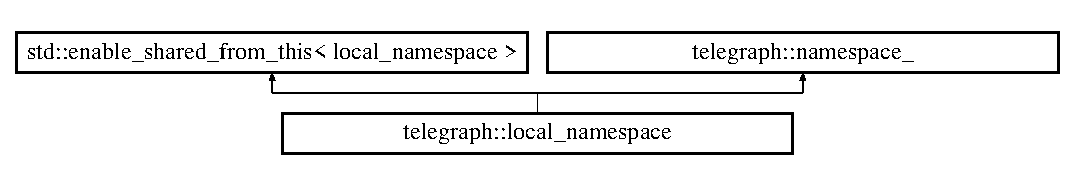
\includegraphics[height=1.830065cm]{classtelegraph_1_1local__namespace}
\end{center}
\end{figure}
\subsection*{Public Member Functions}
\begin{DoxyCompactItemize}
\item 
\hyperlink{classtelegraph_1_1local__namespace_ace7dfdc615015182df5aa9a542833858}{local\+\_\+namespace} (io\+::io\+\_\+context \&ioc)
\item 
void \hyperlink{classtelegraph_1_1local__namespace_a5b322511c2e72c889bcb7ffb5d271d26}{register\+\_\+factory} (const std\+::string \&type, const context\+\_\+factory \&f)
\item 
\hyperlink{namespacetelegraph_a332e681f0d44a1308cf3a013a9dd140f}{context\+\_\+ptr} \hyperlink{classtelegraph_1_1local__namespace_a5ebe002275408c950d8fd44b829434e4}{create} (\hyperlink{structboost_1_1asio_1_1yield__ctx}{io\+::yield\+\_\+ctx} \&yield, const std\+::string\+\_\+view \&name, const std\+::string\+\_\+view \&type, const \hyperlink{classtelegraph_1_1params}{params} \&p) override
\item 
void \hyperlink{classtelegraph_1_1local__namespace_aae3c0b770ea3bd29b1e4dfac7cfd805f}{destroy} (\hyperlink{structboost_1_1asio_1_1yield__ctx}{io\+::yield\+\_\+ctx} \&y, const \hyperlink{namespacetelegraph_a51ee91d7eaeef067f7ccac2b170e5d59}{uuid} \&u) override
\end{DoxyCompactItemize}
\subsection*{Friends}
\begin{DoxyCompactItemize}
\item 
class \hyperlink{classtelegraph_1_1local__namespace_a847a7b7b99bad0f0d4efbbc115fd61f5}{local\+\_\+context}
\end{DoxyCompactItemize}
\subsection*{Additional Inherited Members}


\subsection{Constructor \& Destructor Documentation}
\mbox{\Hypertarget{classtelegraph_1_1local__namespace_ace7dfdc615015182df5aa9a542833858}\label{classtelegraph_1_1local__namespace_ace7dfdc615015182df5aa9a542833858}} 
\index{telegraph\+::local\+\_\+namespace@{telegraph\+::local\+\_\+namespace}!local\+\_\+namespace@{local\+\_\+namespace}}
\index{local\+\_\+namespace@{local\+\_\+namespace}!telegraph\+::local\+\_\+namespace@{telegraph\+::local\+\_\+namespace}}
\subsubsection{\texorpdfstring{local\+\_\+namespace()}{local\_namespace()}}
{\footnotesize\ttfamily telegraph\+::local\+\_\+namespace\+::local\+\_\+namespace (\begin{DoxyParamCaption}\item[{io\+::io\+\_\+context \&}]{ioc }\end{DoxyParamCaption})}



\subsection{Member Function Documentation}
\mbox{\Hypertarget{classtelegraph_1_1local__namespace_a5ebe002275408c950d8fd44b829434e4}\label{classtelegraph_1_1local__namespace_a5ebe002275408c950d8fd44b829434e4}} 
\index{telegraph\+::local\+\_\+namespace@{telegraph\+::local\+\_\+namespace}!create@{create}}
\index{create@{create}!telegraph\+::local\+\_\+namespace@{telegraph\+::local\+\_\+namespace}}
\subsubsection{\texorpdfstring{create()}{create()}}
{\footnotesize\ttfamily \hyperlink{namespacetelegraph_a332e681f0d44a1308cf3a013a9dd140f}{context\+\_\+ptr} telegraph\+::local\+\_\+namespace\+::create (\begin{DoxyParamCaption}\item[{\hyperlink{structboost_1_1asio_1_1yield__ctx}{io\+::yield\+\_\+ctx} \&}]{yield,  }\item[{const std\+::string\+\_\+view \&}]{name,  }\item[{const std\+::string\+\_\+view \&}]{type,  }\item[{const \hyperlink{classtelegraph_1_1params}{params} \&}]{p }\end{DoxyParamCaption})\hspace{0.3cm}{\ttfamily [override]}, {\ttfamily [virtual]}}



Implements \hyperlink{classtelegraph_1_1namespace___ab7a20d98f18494d8e11aada783221dd5}{telegraph\+::namespace\+\_\+}.

\mbox{\Hypertarget{classtelegraph_1_1local__namespace_aae3c0b770ea3bd29b1e4dfac7cfd805f}\label{classtelegraph_1_1local__namespace_aae3c0b770ea3bd29b1e4dfac7cfd805f}} 
\index{telegraph\+::local\+\_\+namespace@{telegraph\+::local\+\_\+namespace}!destroy@{destroy}}
\index{destroy@{destroy}!telegraph\+::local\+\_\+namespace@{telegraph\+::local\+\_\+namespace}}
\subsubsection{\texorpdfstring{destroy()}{destroy()}}
{\footnotesize\ttfamily void telegraph\+::local\+\_\+namespace\+::destroy (\begin{DoxyParamCaption}\item[{\hyperlink{structboost_1_1asio_1_1yield__ctx}{io\+::yield\+\_\+ctx} \&}]{y,  }\item[{const \hyperlink{namespacetelegraph_a51ee91d7eaeef067f7ccac2b170e5d59}{uuid} \&}]{u }\end{DoxyParamCaption})\hspace{0.3cm}{\ttfamily [override]}, {\ttfamily [virtual]}}



Implements \hyperlink{classtelegraph_1_1namespace___ad077446ed8ad4b099ddc050067e14f9d}{telegraph\+::namespace\+\_\+}.

\mbox{\Hypertarget{classtelegraph_1_1local__namespace_a5b322511c2e72c889bcb7ffb5d271d26}\label{classtelegraph_1_1local__namespace_a5b322511c2e72c889bcb7ffb5d271d26}} 
\index{telegraph\+::local\+\_\+namespace@{telegraph\+::local\+\_\+namespace}!register\+\_\+factory@{register\+\_\+factory}}
\index{register\+\_\+factory@{register\+\_\+factory}!telegraph\+::local\+\_\+namespace@{telegraph\+::local\+\_\+namespace}}
\subsubsection{\texorpdfstring{register\+\_\+factory()}{register\_factory()}}
{\footnotesize\ttfamily void telegraph\+::local\+\_\+namespace\+::register\+\_\+factory (\begin{DoxyParamCaption}\item[{const std\+::string \&}]{type,  }\item[{const context\+\_\+factory \&}]{f }\end{DoxyParamCaption})\hspace{0.3cm}{\ttfamily [inline]}}



\subsection{Friends And Related Function Documentation}
\mbox{\Hypertarget{classtelegraph_1_1local__namespace_a847a7b7b99bad0f0d4efbbc115fd61f5}\label{classtelegraph_1_1local__namespace_a847a7b7b99bad0f0d4efbbc115fd61f5}} 
\index{telegraph\+::local\+\_\+namespace@{telegraph\+::local\+\_\+namespace}!local\+\_\+context@{local\+\_\+context}}
\index{local\+\_\+context@{local\+\_\+context}!telegraph\+::local\+\_\+namespace@{telegraph\+::local\+\_\+namespace}}
\subsubsection{\texorpdfstring{local\+\_\+context}{local\_context}}
{\footnotesize\ttfamily friend class \hyperlink{classtelegraph_1_1local__context}{local\+\_\+context}\hspace{0.3cm}{\ttfamily [friend]}}



The documentation for this class was generated from the following files\+:\begin{DoxyCompactItemize}
\item 
\hyperlink{local_2namespace_8hpp}{local/namespace.\+hpp}\item 
\hyperlink{namespace_8cpp}{namespace.\+cpp}\end{DoxyCompactItemize}

\hypertarget{structtelegen_1_1util_1_1make__indexes}{}\section{telegen\+:\+:util\+:\+:make\+\_\+indexes$<$ Types $>$ Struct Template Reference}
\label{structtelegen_1_1util_1_1make__indexes}\index{telegen\+::util\+::make\+\_\+indexes$<$ Types $>$@{telegen\+::util\+::make\+\_\+indexes$<$ Types $>$}}


{\ttfamily \#include $<$util.\+hpp$>$}

Inheritance diagram for telegen\+:\+:util\+:\+:make\+\_\+indexes$<$ Types $>$\+:\begin{figure}[H]
\begin{center}
\leavevmode
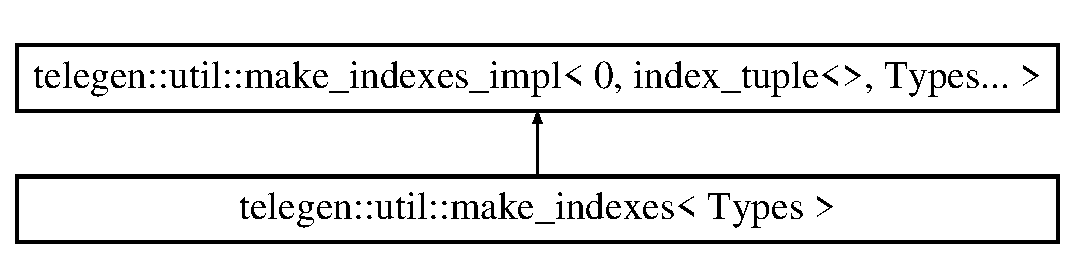
\includegraphics[height=2.000000cm]{structtelegen_1_1util_1_1make__indexes}
\end{center}
\end{figure}


The documentation for this struct was generated from the following file\+:\begin{DoxyCompactItemize}
\item 
\hyperlink{util_8hpp}{util.\+hpp}\end{DoxyCompactItemize}

\hypertarget{structtelegen_1_1util_1_1make__indexes__impl}{}\section{telegen\+:\+:util\+:\+:make\+\_\+indexes\+\_\+impl$<$ I, Index\+Tuple, Types $>$ Struct Template Reference}
\label{structtelegen_1_1util_1_1make__indexes__impl}\index{telegen\+::util\+::make\+\_\+indexes\+\_\+impl$<$ I, Index\+Tuple, Types $>$@{telegen\+::util\+::make\+\_\+indexes\+\_\+impl$<$ I, Index\+Tuple, Types $>$}}


{\ttfamily \#include $<$util.\+hpp$>$}



The documentation for this struct was generated from the following file\+:\begin{DoxyCompactItemize}
\item 
\hyperlink{util_8hpp}{util.\+hpp}\end{DoxyCompactItemize}

\hypertarget{structtelegen_1_1util_1_1make__indexes__impl_3_01I_00_01index__tuple_3_01Indexes_8_8_8_01_4_01_4}{}\section{telegen\+:\+:util\+:\+:make\+\_\+indexes\+\_\+impl$<$ I, index\+\_\+tuple$<$ Indexes... $>$ $>$ Struct Template Reference}
\label{structtelegen_1_1util_1_1make__indexes__impl_3_01I_00_01index__tuple_3_01Indexes_8_8_8_01_4_01_4}\index{telegen\+::util\+::make\+\_\+indexes\+\_\+impl$<$ I, index\+\_\+tuple$<$ Indexes... $>$ $>$@{telegen\+::util\+::make\+\_\+indexes\+\_\+impl$<$ I, index\+\_\+tuple$<$ Indexes... $>$ $>$}}


{\ttfamily \#include $<$util.\+hpp$>$}

\subsection*{Public Types}
\begin{DoxyCompactItemize}
\item 
typedef \hyperlink{structtelegen_1_1util_1_1index__tuple}{index\+\_\+tuple}$<$ Indexes... $>$ \hyperlink{structtelegen_1_1util_1_1make__indexes__impl_3_01I_00_01index__tuple_3_01Indexes_8_8_8_01_4_01_4_a9c2357b6a8e5f7418688518e21a5ac30}{type}
\end{DoxyCompactItemize}


\subsection{Member Typedef Documentation}
\mbox{\Hypertarget{structtelegen_1_1util_1_1make__indexes__impl_3_01I_00_01index__tuple_3_01Indexes_8_8_8_01_4_01_4_a9c2357b6a8e5f7418688518e21a5ac30}\label{structtelegen_1_1util_1_1make__indexes__impl_3_01I_00_01index__tuple_3_01Indexes_8_8_8_01_4_01_4_a9c2357b6a8e5f7418688518e21a5ac30}} 
\index{telegen\+::util\+::make\+\_\+indexes\+\_\+impl$<$ I, index\+\_\+tuple$<$ Indexes... $>$ $>$@{telegen\+::util\+::make\+\_\+indexes\+\_\+impl$<$ I, index\+\_\+tuple$<$ Indexes... $>$ $>$}!type@{type}}
\index{type@{type}!telegen\+::util\+::make\+\_\+indexes\+\_\+impl$<$ I, index\+\_\+tuple$<$ Indexes... $>$ $>$@{telegen\+::util\+::make\+\_\+indexes\+\_\+impl$<$ I, index\+\_\+tuple$<$ Indexes... $>$ $>$}}
\subsubsection{\texorpdfstring{type}{type}}
{\footnotesize\ttfamily template$<$int I, int... Indexes$>$ \\
typedef \hyperlink{structtelegen_1_1util_1_1index__tuple}{index\+\_\+tuple}$<$Indexes...$>$ \hyperlink{structtelegen_1_1util_1_1make__indexes__impl}{telegen\+::util\+::make\+\_\+indexes\+\_\+impl}$<$ I, \hyperlink{structtelegen_1_1util_1_1index__tuple}{index\+\_\+tuple}$<$ Indexes... $>$ $>$\+::\hyperlink{structtelegen_1_1util_1_1make__indexes__impl_3_01I_00_01index__tuple_3_01Indexes_8_8_8_01_4_01_4_a9c2357b6a8e5f7418688518e21a5ac30}{type}}



The documentation for this struct was generated from the following file\+:\begin{DoxyCompactItemize}
\item 
\hyperlink{util_8hpp}{util.\+hpp}\end{DoxyCompactItemize}

\hypertarget{structtelegen_1_1util_1_1make__indexes__impl_3_01I_00_01index__tuple_3_01Indexes_8_8_8_01_4_00_01T_00_01Types_8_8_8_01_4}{}\section{telegen\+:\+:util\+:\+:make\+\_\+indexes\+\_\+impl$<$ I, index\+\_\+tuple$<$ Indexes... $>$, T, Types... $>$ Struct Template Reference}
\label{structtelegen_1_1util_1_1make__indexes__impl_3_01I_00_01index__tuple_3_01Indexes_8_8_8_01_4_00_01T_00_01Types_8_8_8_01_4}\index{telegen\+::util\+::make\+\_\+indexes\+\_\+impl$<$ I, index\+\_\+tuple$<$ Indexes... $>$, T, Types... $>$@{telegen\+::util\+::make\+\_\+indexes\+\_\+impl$<$ I, index\+\_\+tuple$<$ Indexes... $>$, T, Types... $>$}}


{\ttfamily \#include $<$util.\+hpp$>$}

\subsection*{Public Types}
\begin{DoxyCompactItemize}
\item 
typedef \hyperlink{structtelegen_1_1util_1_1make__indexes__impl}{make\+\_\+indexes\+\_\+impl}$<$ I+1, \hyperlink{structtelegen_1_1util_1_1index__tuple}{index\+\_\+tuple}$<$ Indexes..., I $>$, Types... $>$\+::\hyperlink{structtelegen_1_1util_1_1make__indexes__impl_3_01I_00_01index__tuple_3_01Indexes_8_8_8_01_4_00_01T_00_01Types_8_8_8_01_4_a5046a04e998e0bd21d60e07ed6ad6b0e}{type} \hyperlink{structtelegen_1_1util_1_1make__indexes__impl_3_01I_00_01index__tuple_3_01Indexes_8_8_8_01_4_00_01T_00_01Types_8_8_8_01_4_a5046a04e998e0bd21d60e07ed6ad6b0e}{type}
\end{DoxyCompactItemize}


\subsection{Member Typedef Documentation}
\mbox{\Hypertarget{structtelegen_1_1util_1_1make__indexes__impl_3_01I_00_01index__tuple_3_01Indexes_8_8_8_01_4_00_01T_00_01Types_8_8_8_01_4_a5046a04e998e0bd21d60e07ed6ad6b0e}\label{structtelegen_1_1util_1_1make__indexes__impl_3_01I_00_01index__tuple_3_01Indexes_8_8_8_01_4_00_01T_00_01Types_8_8_8_01_4_a5046a04e998e0bd21d60e07ed6ad6b0e}} 
\index{telegen\+::util\+::make\+\_\+indexes\+\_\+impl$<$ I, index\+\_\+tuple$<$ Indexes... $>$, T, Types... $>$@{telegen\+::util\+::make\+\_\+indexes\+\_\+impl$<$ I, index\+\_\+tuple$<$ Indexes... $>$, T, Types... $>$}!type@{type}}
\index{type@{type}!telegen\+::util\+::make\+\_\+indexes\+\_\+impl$<$ I, index\+\_\+tuple$<$ Indexes... $>$, T, Types... $>$@{telegen\+::util\+::make\+\_\+indexes\+\_\+impl$<$ I, index\+\_\+tuple$<$ Indexes... $>$, T, Types... $>$}}
\subsubsection{\texorpdfstring{type}{type}}
{\footnotesize\ttfamily template$<$int I, int... Indexes, typename T , typename ... Types$>$ \\
typedef \hyperlink{structtelegen_1_1util_1_1make__indexes__impl}{make\+\_\+indexes\+\_\+impl}$<$I + 1, \hyperlink{structtelegen_1_1util_1_1index__tuple}{index\+\_\+tuple}$<$Indexes..., I$>$, Types...$>$\+::\hyperlink{structtelegen_1_1util_1_1make__indexes__impl_3_01I_00_01index__tuple_3_01Indexes_8_8_8_01_4_00_01T_00_01Types_8_8_8_01_4_a5046a04e998e0bd21d60e07ed6ad6b0e}{type} \hyperlink{structtelegen_1_1util_1_1make__indexes__impl}{telegen\+::util\+::make\+\_\+indexes\+\_\+impl}$<$ I, \hyperlink{structtelegen_1_1util_1_1index__tuple}{index\+\_\+tuple}$<$ Indexes... $>$, T, Types... $>$\+::\hyperlink{structtelegen_1_1util_1_1make__indexes__impl_3_01I_00_01index__tuple_3_01Indexes_8_8_8_01_4_00_01T_00_01Types_8_8_8_01_4_a5046a04e998e0bd21d60e07ed6ad6b0e}{type}}



The documentation for this struct was generated from the following file\+:\begin{DoxyCompactItemize}
\item 
\hyperlink{util_8hpp}{util.\+hpp}\end{DoxyCompactItemize}

\hypertarget{classtelegraph_1_1missing__error}{}\section{telegraph\+:\+:missing\+\_\+error Class Reference}
\label{classtelegraph_1_1missing__error}\index{telegraph\+::missing\+\_\+error@{telegraph\+::missing\+\_\+error}}


{\ttfamily \#include $<$errors.\+hpp$>$}

Inheritance diagram for telegraph\+:\+:missing\+\_\+error\+:\begin{figure}[H]
\begin{center}
\leavevmode
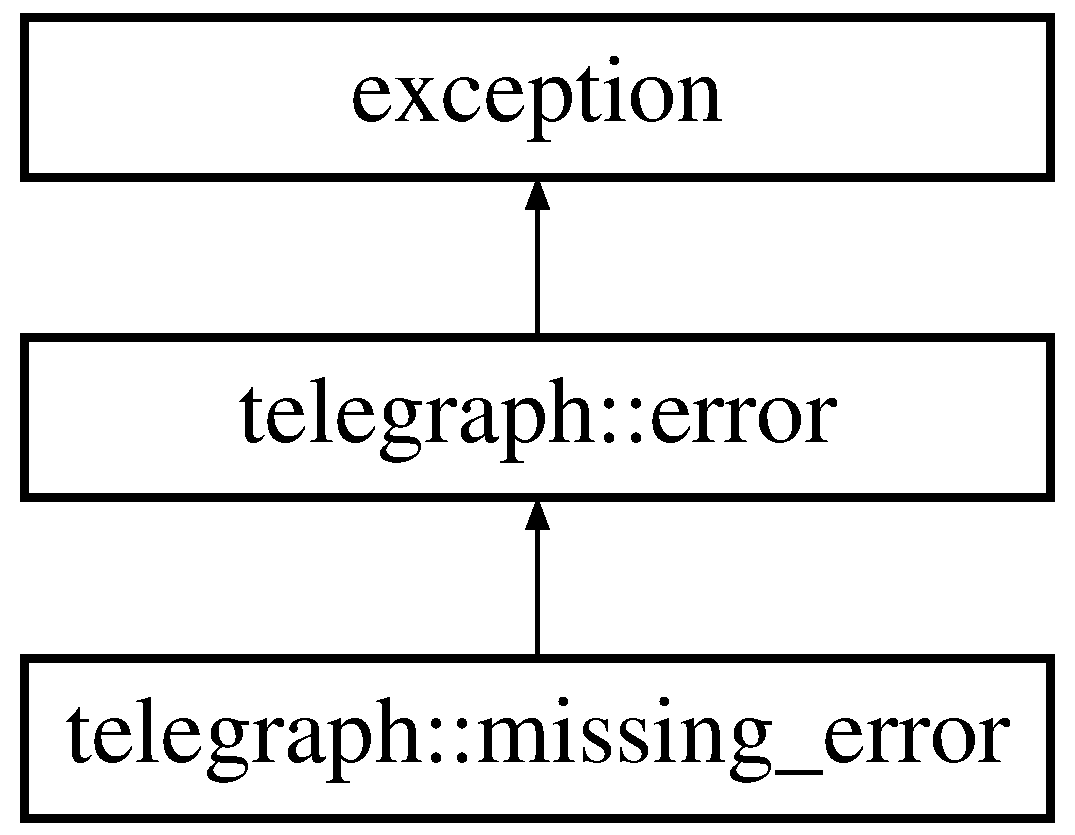
\includegraphics[height=3.000000cm]{classtelegraph_1_1missing__error}
\end{center}
\end{figure}
\subsection*{Public Member Functions}
\begin{DoxyCompactItemize}
\item 
\hyperlink{classtelegraph_1_1missing__error_a886bea805b734808fee6f0066375480c}{missing\+\_\+error} (const std\+::string\+\_\+view \&m)
\end{DoxyCompactItemize}


\subsection{Constructor \& Destructor Documentation}
\mbox{\Hypertarget{classtelegraph_1_1missing__error_a886bea805b734808fee6f0066375480c}\label{classtelegraph_1_1missing__error_a886bea805b734808fee6f0066375480c}} 
\index{telegraph\+::missing\+\_\+error@{telegraph\+::missing\+\_\+error}!missing\+\_\+error@{missing\+\_\+error}}
\index{missing\+\_\+error@{missing\+\_\+error}!telegraph\+::missing\+\_\+error@{telegraph\+::missing\+\_\+error}}
\subsubsection{\texorpdfstring{missing\+\_\+error()}{missing\_error()}}
{\footnotesize\ttfamily telegraph\+::missing\+\_\+error\+::missing\+\_\+error (\begin{DoxyParamCaption}\item[{const std\+::string\+\_\+view \&}]{m }\end{DoxyParamCaption})\hspace{0.3cm}{\ttfamily [inline]}}



The documentation for this class was generated from the following file\+:\begin{DoxyCompactItemize}
\item 
\hyperlink{errors_8hpp}{errors.\+hpp}\end{DoxyCompactItemize}

\hypertarget{classtelegraph_1_1namespace__}{}\section{telegraph\+:\+:namespace\+\_\+ Class Reference}
\label{classtelegraph_1_1namespace__}\index{telegraph\+::namespace\+\_\+@{telegraph\+::namespace\+\_\+}}


{\ttfamily \#include $<$namespace.\+hpp$>$}

Inheritance diagram for telegraph\+:\+:namespace\+\_\+\+:\begin{figure}[H]
\begin{center}
\leavevmode
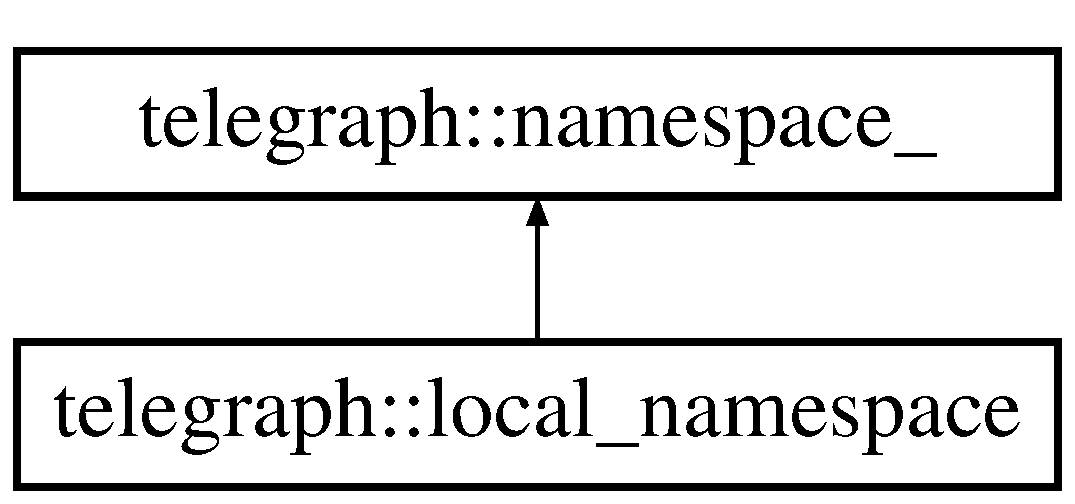
\includegraphics[height=2.000000cm]{classtelegraph_1_1namespace__}
\end{center}
\end{figure}
\subsection*{Public Member Functions}
\begin{DoxyCompactItemize}
\item 
\hyperlink{classtelegraph_1_1namespace___a0ea0a99c1d31a5e867ccd0bd8f3d0917}{namespace\+\_\+} ()
\item 
virtual \hyperlink{namespacetelegraph_a332e681f0d44a1308cf3a013a9dd140f}{context\+\_\+ptr} \hyperlink{classtelegraph_1_1namespace___ab7a20d98f18494d8e11aada783221dd5}{create} (\hyperlink{structboost_1_1asio_1_1yield__ctx}{io\+::yield\+\_\+ctx} \&, const std\+::string\+\_\+view \&name, const std\+::string\+\_\+view \&type, const \hyperlink{classtelegraph_1_1params}{params} \&p)=0
\item 
virtual void \hyperlink{classtelegraph_1_1namespace___ad077446ed8ad4b099ddc050067e14f9d}{destroy} (\hyperlink{structboost_1_1asio_1_1yield__ctx}{io\+::yield\+\_\+ctx} \&, const \hyperlink{namespacetelegraph_a51ee91d7eaeef067f7ccac2b170e5d59}{uuid} \&u)=0
\end{DoxyCompactItemize}
\subsection*{Public Attributes}
\begin{DoxyCompactItemize}
\item 
\hyperlink{namespacetelegraph_a4fa3678b3fd260dc79a98bea50d582fd}{collection\+\_\+ptr}$<$ \hyperlink{namespacetelegraph_a332e681f0d44a1308cf3a013a9dd140f}{context\+\_\+ptr} $>$ \hyperlink{classtelegraph_1_1namespace___a04ffdef6fc2b8c0ed4b02ba3f039b27a}{contexts}
\end{DoxyCompactItemize}


\subsection{Constructor \& Destructor Documentation}
\mbox{\Hypertarget{classtelegraph_1_1namespace___a0ea0a99c1d31a5e867ccd0bd8f3d0917}\label{classtelegraph_1_1namespace___a0ea0a99c1d31a5e867ccd0bd8f3d0917}} 
\index{telegraph\+::namespace\+\_\+@{telegraph\+::namespace\+\_\+}!namespace\+\_\+@{namespace\+\_\+}}
\index{namespace\+\_\+@{namespace\+\_\+}!telegraph\+::namespace\+\_\+@{telegraph\+::namespace\+\_\+}}
\subsubsection{\texorpdfstring{namespace\+\_\+()}{namespace\_()}}
{\footnotesize\ttfamily telegraph\+::namespace\+\_\+\+::namespace\+\_\+ (\begin{DoxyParamCaption}{ }\end{DoxyParamCaption})\hspace{0.3cm}{\ttfamily [inline]}}



\subsection{Member Function Documentation}
\mbox{\Hypertarget{classtelegraph_1_1namespace___ab7a20d98f18494d8e11aada783221dd5}\label{classtelegraph_1_1namespace___ab7a20d98f18494d8e11aada783221dd5}} 
\index{telegraph\+::namespace\+\_\+@{telegraph\+::namespace\+\_\+}!create@{create}}
\index{create@{create}!telegraph\+::namespace\+\_\+@{telegraph\+::namespace\+\_\+}}
\subsubsection{\texorpdfstring{create()}{create()}}
{\footnotesize\ttfamily virtual \hyperlink{namespacetelegraph_a332e681f0d44a1308cf3a013a9dd140f}{context\+\_\+ptr} telegraph\+::namespace\+\_\+\+::create (\begin{DoxyParamCaption}\item[{\hyperlink{structboost_1_1asio_1_1yield__ctx}{io\+::yield\+\_\+ctx} \&}]{,  }\item[{const std\+::string\+\_\+view \&}]{name,  }\item[{const std\+::string\+\_\+view \&}]{type,  }\item[{const \hyperlink{classtelegraph_1_1params}{params} \&}]{p }\end{DoxyParamCaption})\hspace{0.3cm}{\ttfamily [pure virtual]}}



Implemented in \hyperlink{classtelegraph_1_1local__namespace_a5ebe002275408c950d8fd44b829434e4}{telegraph\+::local\+\_\+namespace}.

\mbox{\Hypertarget{classtelegraph_1_1namespace___ad077446ed8ad4b099ddc050067e14f9d}\label{classtelegraph_1_1namespace___ad077446ed8ad4b099ddc050067e14f9d}} 
\index{telegraph\+::namespace\+\_\+@{telegraph\+::namespace\+\_\+}!destroy@{destroy}}
\index{destroy@{destroy}!telegraph\+::namespace\+\_\+@{telegraph\+::namespace\+\_\+}}
\subsubsection{\texorpdfstring{destroy()}{destroy()}}
{\footnotesize\ttfamily virtual void telegraph\+::namespace\+\_\+\+::destroy (\begin{DoxyParamCaption}\item[{\hyperlink{structboost_1_1asio_1_1yield__ctx}{io\+::yield\+\_\+ctx} \&}]{,  }\item[{const \hyperlink{namespacetelegraph_a51ee91d7eaeef067f7ccac2b170e5d59}{uuid} \&}]{u }\end{DoxyParamCaption})\hspace{0.3cm}{\ttfamily [pure virtual]}}



Implemented in \hyperlink{classtelegraph_1_1local__namespace_aae3c0b770ea3bd29b1e4dfac7cfd805f}{telegraph\+::local\+\_\+namespace}.



\subsection{Member Data Documentation}
\mbox{\Hypertarget{classtelegraph_1_1namespace___a04ffdef6fc2b8c0ed4b02ba3f039b27a}\label{classtelegraph_1_1namespace___a04ffdef6fc2b8c0ed4b02ba3f039b27a}} 
\index{telegraph\+::namespace\+\_\+@{telegraph\+::namespace\+\_\+}!contexts@{contexts}}
\index{contexts@{contexts}!telegraph\+::namespace\+\_\+@{telegraph\+::namespace\+\_\+}}
\subsubsection{\texorpdfstring{contexts}{contexts}}
{\footnotesize\ttfamily \hyperlink{namespacetelegraph_a4fa3678b3fd260dc79a98bea50d582fd}{collection\+\_\+ptr}$<$\hyperlink{namespacetelegraph_a332e681f0d44a1308cf3a013a9dd140f}{context\+\_\+ptr}$>$ telegraph\+::namespace\+\_\+\+::contexts}



The documentation for this class was generated from the following file\+:\begin{DoxyCompactItemize}
\item 
\hyperlink{common_2namespace_8hpp}{common/namespace.\+hpp}\end{DoxyCompactItemize}

\hypertarget{classtelegen_1_1node}{}\section{telegen\+:\+:node Class Reference}
\label{classtelegen_1_1node}\index{telegen\+::node@{telegen\+::node}}


{\ttfamily \#include $<$nodes.\+hpp$>$}

Inheritance diagram for telegen\+:\+:node\+:\begin{figure}[H]
\begin{center}
\leavevmode
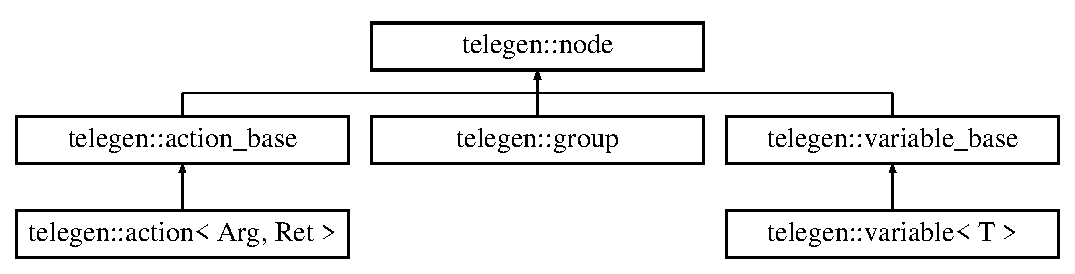
\includegraphics[height=3.000000cm]{classtelegen_1_1node}
\end{center}
\end{figure}
\subsection*{Public Types}
\begin{DoxyCompactItemize}
\item 
using \hyperlink{classtelegen_1_1node_aae3ff0d12932c55fdc88a1743e27ea56}{id} = uint16\+\_\+t
\end{DoxyCompactItemize}
\subsection*{Public Member Functions}
\begin{DoxyCompactItemize}
\item 
constexpr \hyperlink{classtelegen_1_1node_ae046ceb8c032f5655160173c0777dba8}{node} (\hyperlink{classtelegen_1_1node_aae3ff0d12932c55fdc88a1743e27ea56}{id} i, const char $\ast$name, const char $\ast$pretty, const char $\ast$desc)
\item 
constexpr \hyperlink{classtelegen_1_1node_aae3ff0d12932c55fdc88a1743e27ea56}{id} \hyperlink{classtelegen_1_1node_a9e94c3554697bb443e67316170815eed}{get\+\_\+id} () const
\item 
constexpr const char $\ast$ \hyperlink{classtelegen_1_1node_afc6c76d81436f9040668324ed2d65ce4}{get\+\_\+name} () const
\item 
constexpr const char $\ast$ \hyperlink{classtelegen_1_1node_aa92b0c42b744508c2b39bc047051a3ec}{get\+\_\+pretty} () const
\item 
constexpr const char $\ast$ \hyperlink{classtelegen_1_1node_a9393b332196fe1a8458d85308f8551d5}{get\+\_\+desc} () const
\item 
virtual void \hyperlink{classtelegen_1_1node_a8b6169d62f6e7c2e301435e52442fed3}{pack} (telegraph\+\_\+\+Node $\ast$n) const =0
\item 
constexpr void \hyperlink{classtelegen_1_1node_a33a4f88e44337dcf2885e3e787970db7}{set\+\_\+owner} (\hyperlink{classtelegen_1_1source}{source} $\ast$i)
\end{DoxyCompactItemize}
\subsection*{Protected Attributes}
\begin{DoxyCompactItemize}
\item 
\hyperlink{classtelegen_1_1source}{source} $\ast$ \hyperlink{classtelegen_1_1node_ab97909f583b8777e9b95f11edfc869a8}{owner\+\_\+}
\item 
const \hyperlink{classtelegen_1_1node_aae3ff0d12932c55fdc88a1743e27ea56}{id} \hyperlink{classtelegen_1_1node_a0f485aa38b6a5a1e0ca55fd1f493e141}{id\+\_\+}
\item 
const char $\ast$const \hyperlink{classtelegen_1_1node_abb59d672031a10b796e44d628bb835be}{name\+\_\+}
\item 
const char $\ast$const \hyperlink{classtelegen_1_1node_abfa84da09528702afb75b46771ab9dcd}{pretty\+\_\+}
\item 
const char $\ast$const \hyperlink{classtelegen_1_1node_ab9842f580e8e37753a42565793a455fc}{desc\+\_\+}
\end{DoxyCompactItemize}


\subsection{Member Typedef Documentation}
\mbox{\Hypertarget{classtelegen_1_1node_aae3ff0d12932c55fdc88a1743e27ea56}\label{classtelegen_1_1node_aae3ff0d12932c55fdc88a1743e27ea56}} 
\index{telegen\+::node@{telegen\+::node}!id@{id}}
\index{id@{id}!telegen\+::node@{telegen\+::node}}
\subsubsection{\texorpdfstring{id}{id}}
{\footnotesize\ttfamily using \hyperlink{classtelegen_1_1node_aae3ff0d12932c55fdc88a1743e27ea56}{telegen\+::node\+::id} =  uint16\+\_\+t}



\subsection{Constructor \& Destructor Documentation}
\mbox{\Hypertarget{classtelegen_1_1node_ae046ceb8c032f5655160173c0777dba8}\label{classtelegen_1_1node_ae046ceb8c032f5655160173c0777dba8}} 
\index{telegen\+::node@{telegen\+::node}!node@{node}}
\index{node@{node}!telegen\+::node@{telegen\+::node}}
\subsubsection{\texorpdfstring{node()}{node()}}
{\footnotesize\ttfamily constexpr telegen\+::node\+::node (\begin{DoxyParamCaption}\item[{\hyperlink{classtelegen_1_1node_aae3ff0d12932c55fdc88a1743e27ea56}{id}}]{i,  }\item[{const char $\ast$}]{name,  }\item[{const char $\ast$}]{pretty,  }\item[{const char $\ast$}]{desc }\end{DoxyParamCaption})\hspace{0.3cm}{\ttfamily [inline]}}



\subsection{Member Function Documentation}
\mbox{\Hypertarget{classtelegen_1_1node_a9393b332196fe1a8458d85308f8551d5}\label{classtelegen_1_1node_a9393b332196fe1a8458d85308f8551d5}} 
\index{telegen\+::node@{telegen\+::node}!get\+\_\+desc@{get\+\_\+desc}}
\index{get\+\_\+desc@{get\+\_\+desc}!telegen\+::node@{telegen\+::node}}
\subsubsection{\texorpdfstring{get\+\_\+desc()}{get\_desc()}}
{\footnotesize\ttfamily constexpr const char$\ast$ telegen\+::node\+::get\+\_\+desc (\begin{DoxyParamCaption}{ }\end{DoxyParamCaption}) const\hspace{0.3cm}{\ttfamily [inline]}}

\mbox{\Hypertarget{classtelegen_1_1node_a9e94c3554697bb443e67316170815eed}\label{classtelegen_1_1node_a9e94c3554697bb443e67316170815eed}} 
\index{telegen\+::node@{telegen\+::node}!get\+\_\+id@{get\+\_\+id}}
\index{get\+\_\+id@{get\+\_\+id}!telegen\+::node@{telegen\+::node}}
\subsubsection{\texorpdfstring{get\+\_\+id()}{get\_id()}}
{\footnotesize\ttfamily constexpr \hyperlink{classtelegen_1_1node_aae3ff0d12932c55fdc88a1743e27ea56}{id} telegen\+::node\+::get\+\_\+id (\begin{DoxyParamCaption}{ }\end{DoxyParamCaption}) const\hspace{0.3cm}{\ttfamily [inline]}}

\mbox{\Hypertarget{classtelegen_1_1node_afc6c76d81436f9040668324ed2d65ce4}\label{classtelegen_1_1node_afc6c76d81436f9040668324ed2d65ce4}} 
\index{telegen\+::node@{telegen\+::node}!get\+\_\+name@{get\+\_\+name}}
\index{get\+\_\+name@{get\+\_\+name}!telegen\+::node@{telegen\+::node}}
\subsubsection{\texorpdfstring{get\+\_\+name()}{get\_name()}}
{\footnotesize\ttfamily constexpr const char$\ast$ telegen\+::node\+::get\+\_\+name (\begin{DoxyParamCaption}{ }\end{DoxyParamCaption}) const\hspace{0.3cm}{\ttfamily [inline]}}

\mbox{\Hypertarget{classtelegen_1_1node_aa92b0c42b744508c2b39bc047051a3ec}\label{classtelegen_1_1node_aa92b0c42b744508c2b39bc047051a3ec}} 
\index{telegen\+::node@{telegen\+::node}!get\+\_\+pretty@{get\+\_\+pretty}}
\index{get\+\_\+pretty@{get\+\_\+pretty}!telegen\+::node@{telegen\+::node}}
\subsubsection{\texorpdfstring{get\+\_\+pretty()}{get\_pretty()}}
{\footnotesize\ttfamily constexpr const char$\ast$ telegen\+::node\+::get\+\_\+pretty (\begin{DoxyParamCaption}{ }\end{DoxyParamCaption}) const\hspace{0.3cm}{\ttfamily [inline]}}

\mbox{\Hypertarget{classtelegen_1_1node_a8b6169d62f6e7c2e301435e52442fed3}\label{classtelegen_1_1node_a8b6169d62f6e7c2e301435e52442fed3}} 
\index{telegen\+::node@{telegen\+::node}!pack@{pack}}
\index{pack@{pack}!telegen\+::node@{telegen\+::node}}
\subsubsection{\texorpdfstring{pack()}{pack()}}
{\footnotesize\ttfamily virtual void telegen\+::node\+::pack (\begin{DoxyParamCaption}\item[{telegraph\+\_\+\+Node $\ast$}]{n }\end{DoxyParamCaption}) const\hspace{0.3cm}{\ttfamily [pure virtual]}}



Implemented in \hyperlink{classtelegen_1_1variable_a8a077a32a045a67f049737517be3ea51}{telegen\+::variable$<$ T $>$}, \hyperlink{classtelegen_1_1action_a0e5686b3bf433afab1b0fda1002f95b0}{telegen\+::action$<$ Arg, Ret $>$}, and \hyperlink{classtelegen_1_1group_ae146155bf745b0b3d39e3244c3ebb26d}{telegen\+::group}.

\mbox{\Hypertarget{classtelegen_1_1node_a33a4f88e44337dcf2885e3e787970db7}\label{classtelegen_1_1node_a33a4f88e44337dcf2885e3e787970db7}} 
\index{telegen\+::node@{telegen\+::node}!set\+\_\+owner@{set\+\_\+owner}}
\index{set\+\_\+owner@{set\+\_\+owner}!telegen\+::node@{telegen\+::node}}
\subsubsection{\texorpdfstring{set\+\_\+owner()}{set\_owner()}}
{\footnotesize\ttfamily constexpr void telegen\+::node\+::set\+\_\+owner (\begin{DoxyParamCaption}\item[{\hyperlink{classtelegen_1_1source}{source} $\ast$}]{i }\end{DoxyParamCaption})\hspace{0.3cm}{\ttfamily [inline]}}



\subsection{Member Data Documentation}
\mbox{\Hypertarget{classtelegen_1_1node_ab9842f580e8e37753a42565793a455fc}\label{classtelegen_1_1node_ab9842f580e8e37753a42565793a455fc}} 
\index{telegen\+::node@{telegen\+::node}!desc\+\_\+@{desc\+\_\+}}
\index{desc\+\_\+@{desc\+\_\+}!telegen\+::node@{telegen\+::node}}
\subsubsection{\texorpdfstring{desc\+\_\+}{desc\_}}
{\footnotesize\ttfamily const char$\ast$ const telegen\+::node\+::desc\+\_\+\hspace{0.3cm}{\ttfamily [protected]}}

\mbox{\Hypertarget{classtelegen_1_1node_a0f485aa38b6a5a1e0ca55fd1f493e141}\label{classtelegen_1_1node_a0f485aa38b6a5a1e0ca55fd1f493e141}} 
\index{telegen\+::node@{telegen\+::node}!id\+\_\+@{id\+\_\+}}
\index{id\+\_\+@{id\+\_\+}!telegen\+::node@{telegen\+::node}}
\subsubsection{\texorpdfstring{id\+\_\+}{id\_}}
{\footnotesize\ttfamily const \hyperlink{classtelegen_1_1node_aae3ff0d12932c55fdc88a1743e27ea56}{id} telegen\+::node\+::id\+\_\+\hspace{0.3cm}{\ttfamily [protected]}}

\mbox{\Hypertarget{classtelegen_1_1node_abb59d672031a10b796e44d628bb835be}\label{classtelegen_1_1node_abb59d672031a10b796e44d628bb835be}} 
\index{telegen\+::node@{telegen\+::node}!name\+\_\+@{name\+\_\+}}
\index{name\+\_\+@{name\+\_\+}!telegen\+::node@{telegen\+::node}}
\subsubsection{\texorpdfstring{name\+\_\+}{name\_}}
{\footnotesize\ttfamily const char$\ast$ const telegen\+::node\+::name\+\_\+\hspace{0.3cm}{\ttfamily [protected]}}

\mbox{\Hypertarget{classtelegen_1_1node_ab97909f583b8777e9b95f11edfc869a8}\label{classtelegen_1_1node_ab97909f583b8777e9b95f11edfc869a8}} 
\index{telegen\+::node@{telegen\+::node}!owner\+\_\+@{owner\+\_\+}}
\index{owner\+\_\+@{owner\+\_\+}!telegen\+::node@{telegen\+::node}}
\subsubsection{\texorpdfstring{owner\+\_\+}{owner\_}}
{\footnotesize\ttfamily \hyperlink{classtelegen_1_1source}{source}$\ast$ telegen\+::node\+::owner\+\_\+\hspace{0.3cm}{\ttfamily [protected]}}

\mbox{\Hypertarget{classtelegen_1_1node_abfa84da09528702afb75b46771ab9dcd}\label{classtelegen_1_1node_abfa84da09528702afb75b46771ab9dcd}} 
\index{telegen\+::node@{telegen\+::node}!pretty\+\_\+@{pretty\+\_\+}}
\index{pretty\+\_\+@{pretty\+\_\+}!telegen\+::node@{telegen\+::node}}
\subsubsection{\texorpdfstring{pretty\+\_\+}{pretty\_}}
{\footnotesize\ttfamily const char$\ast$ const telegen\+::node\+::pretty\+\_\+\hspace{0.3cm}{\ttfamily [protected]}}



The documentation for this class was generated from the following file\+:\begin{DoxyCompactItemize}
\item 
\hyperlink{gen_2telegen_2nodes_8hpp}{gen/telegen/nodes.\+hpp}\end{DoxyCompactItemize}

\hypertarget{classtelegraph_1_1node}{}\section{telegraph\+:\+:node Class Reference}
\label{classtelegraph_1_1node}\index{telegraph\+::node@{telegraph\+::node}}


{\ttfamily \#include $<$nodes.\+hpp$>$}

Inheritance diagram for telegraph\+:\+:node\+:\begin{figure}[H]
\begin{center}
\leavevmode
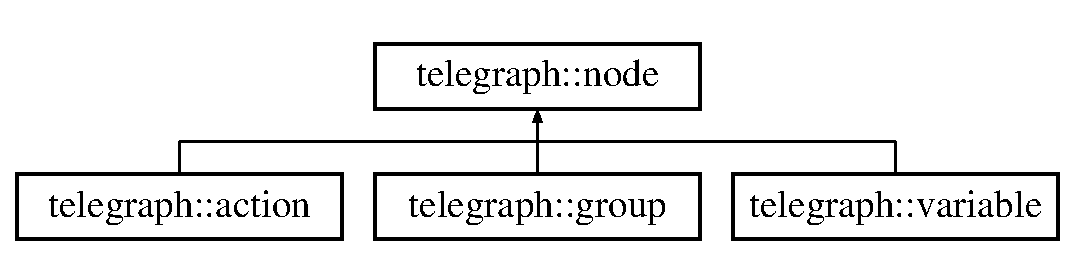
\includegraphics[height=2.000000cm]{classtelegraph_1_1node}
\end{center}
\end{figure}
\subsection*{Public Types}
\begin{DoxyCompactItemize}
\item 
using \hyperlink{classtelegraph_1_1node_a90bc576d668ed141d5354a06aa9c8d9a}{id} = uint16\+\_\+t
\end{DoxyCompactItemize}
\subsection*{Public Member Functions}
\begin{DoxyCompactItemize}
\item 
\hyperlink{classtelegraph_1_1node_a6891eb034aa7d988f1459d3ed2bc0106}{node} (\hyperlink{classtelegraph_1_1node_a90bc576d668ed141d5354a06aa9c8d9a}{id} i, const std\+::string\+\_\+view \&name, const std\+::string\+\_\+view \&pretty, const std\+::string\+\_\+view \&desc)
\item 
\hyperlink{classtelegraph_1_1node_a76746ee2232620309c5f60ca94af24ee}{node} (const \hyperlink{classtelegraph_1_1node}{node} \&n)
\item 
virtual \hyperlink{classtelegraph_1_1node_a7fe858c56729feae1e92625ff4827209}{$\sim$node} ()
\item 
\hyperlink{classtelegraph_1_1node}{node} \& \hyperlink{classtelegraph_1_1node_aa7aacc23330b9b8f98b05f8155481de7}{operator=} (const \hyperlink{classtelegraph_1_1node}{node} \&n)=delete
\item 
constexpr const \hyperlink{classtelegraph_1_1node_a90bc576d668ed141d5354a06aa9c8d9a}{id} \hyperlink{classtelegraph_1_1node_a8067bd46e650371084576234acfb8289}{get\+\_\+id} () const
\item 
constexpr const std\+::string \& \hyperlink{classtelegraph_1_1node_af33c56a0a2d2340c9cae412017a4fa4f}{get\+\_\+name} () const
\item 
constexpr const std\+::string \& \hyperlink{classtelegraph_1_1node_abeaa41162d9369bc6fc8bcbabe9d23e3}{get\+\_\+pretty} () const
\item 
constexpr const std\+::string \& \hyperlink{classtelegraph_1_1node_aff9478f841f7f791af1cd60513877440}{get\+\_\+desc} () const
\item 
constexpr \hyperlink{classtelegraph_1_1group}{group} $\ast$ \hyperlink{classtelegraph_1_1node_a2bcd9175c2e3b667422d86fc6fcc9959}{get\+\_\+parent} ()
\item 
constexpr const \hyperlink{classtelegraph_1_1group}{group} $\ast$ \hyperlink{classtelegraph_1_1node_adb0c016733fe55621b061d4e81d296fa}{get\+\_\+parent} () const
\item 
std\+::string \hyperlink{classtelegraph_1_1node_a3cb6dfaddab4d5953c04bb5ec348763b}{topic} () const
\item 
std\+::vector$<$ std\+::string $>$ \hyperlink{classtelegraph_1_1node_a1f1a005517baad53ec2407c27a13c9c4}{path} () const
\item 
virtual \hyperlink{classtelegraph_1_1node}{node} $\ast$ \hyperlink{classtelegraph_1_1node_a2d5ea5366a04f3b3841de9bc21e70416}{from\+\_\+path} (const std\+::vector$<$ std\+::string\+\_\+view $>$ \&p, size\+\_\+t idx=0)
\item 
virtual const \hyperlink{classtelegraph_1_1node}{node} $\ast$ \hyperlink{classtelegraph_1_1node_aaba33e2aa28a99dcd8f4b1888c3a5706}{from\+\_\+path} (const std\+::vector$<$ std\+::string\+\_\+view $>$ \&p, size\+\_\+t idx=0) const
\item 
virtual std\+::vector$<$ \hyperlink{classtelegraph_1_1node}{node} $\ast$ $>$ \hyperlink{classtelegraph_1_1node_a14eb2051c1efaf4de6684d3e50aebeb7}{nodes} ()
\item 
virtual std\+::vector$<$ const \hyperlink{classtelegraph_1_1node}{node} $\ast$ $>$ \hyperlink{classtelegraph_1_1node_a9d19888a9a73a4623dcab55be6386395}{nodes} () const
\item 
virtual \hyperlink{classtelegraph_1_1node}{node} $\ast$ \hyperlink{classtelegraph_1_1node_ad82c9a9af7b7cf132db1c1e74f09254f}{operator\mbox{[}$\,$\mbox{]}} (size\+\_\+t idx)
\item 
virtual const \hyperlink{classtelegraph_1_1node}{node} $\ast$ \hyperlink{classtelegraph_1_1node_a4a2a451694b0a4b2c4ec26eee02e46ad}{operator\mbox{[}$\,$\mbox{]}} (size\+\_\+t idx) const
\item 
virtual \hyperlink{classtelegraph_1_1node}{node} $\ast$ \hyperlink{classtelegraph_1_1node_a3cf657c57fe639f6288f2acdd9b50e3c}{operator\mbox{[}$\,$\mbox{]}} (const std\+::string \&child)
\item 
virtual const \hyperlink{classtelegraph_1_1node}{node} $\ast$ \hyperlink{classtelegraph_1_1node_aad6b0bbccc9831f82117a1cc03493f6c}{operator\mbox{[}$\,$\mbox{]}} (const std\+::string \&child) const
\item 
virtual void \hyperlink{classtelegraph_1_1node_a6d864584bfadd3520194066f8b62812b}{set\+\_\+owner} (const std\+::weak\+\_\+ptr$<$ \hyperlink{classtelegraph_1_1context}{context} $>$ \&c)
\item 
virtual void \hyperlink{classtelegraph_1_1node_ac0bbcb9d810a2cca87b120301c0972a0}{set\+\_\+unowned} ()
\item 
virtual bool \hyperlink{classtelegraph_1_1node_a68c4aed1434da1f0ece9089ff99ffcdb}{compatible\+\_\+with} (\hyperlink{classtelegraph_1_1node}{node} $\ast$other) const =0
\item 
virtual void \hyperlink{classtelegraph_1_1node_a5006b21e9b83ecd52f3f953a1b828773}{pack} (Node $\ast$proto) const =0
\item 
virtual std\+::unique\+\_\+ptr$<$ \hyperlink{classtelegraph_1_1node}{node} $>$ \hyperlink{classtelegraph_1_1node_ae90515f4573cfa43c168cba9d542df6b}{clone} () const =0
\end{DoxyCompactItemize}
\subsection*{Static Public Member Functions}
\begin{DoxyCompactItemize}
\item 
static \hyperlink{classtelegraph_1_1node}{node} $\ast$ \hyperlink{classtelegraph_1_1node_a2a2ddaf1b7210b1e69f63adcc1d83fa5}{unpack} (const Node \&proto)
\end{DoxyCompactItemize}
\subsection*{Protected Member Functions}
\begin{DoxyCompactItemize}
\item 
constexpr void \hyperlink{classtelegraph_1_1node_ae0f1bd6f97ea3e1f21940a7eebb70fab}{set\+\_\+parent} (\hyperlink{classtelegraph_1_1group}{group} $\ast$g)
\item 
virtual void \hyperlink{classtelegraph_1_1node_a70ae6b3d07132abcc4022a7ac9facf6b}{print} (std\+::ostream \&o, int ident=0) const
\end{DoxyCompactItemize}
\subsection*{Protected Attributes}
\begin{DoxyCompactItemize}
\item 
\hyperlink{classtelegraph_1_1node_a90bc576d668ed141d5354a06aa9c8d9a}{id} \hyperlink{classtelegraph_1_1node_abbc7178e6f854f475ac04fab89afe8ed}{id\+\_\+}
\item 
std\+::string \hyperlink{classtelegraph_1_1node_a14e3a8896e5cda1ad3e91186009e4a83}{name\+\_\+}
\item 
std\+::string \hyperlink{classtelegraph_1_1node_a6d308459f7de904b54a1a551b3be5cb7}{pretty\+\_\+}
\item 
std\+::string \hyperlink{classtelegraph_1_1node_ade724e97cdd76b83c5de499b62f91ecb}{desc\+\_\+}
\item 
\hyperlink{classtelegraph_1_1group}{group} $\ast$ \hyperlink{classtelegraph_1_1node_a875057ad03af20786456cffe6d5b22d9}{parent\+\_\+}
\item 
std\+::weak\+\_\+ptr$<$ \hyperlink{classtelegraph_1_1context}{context} $>$ \hyperlink{classtelegraph_1_1node_a5419854e28d2b852ecaf964849220f9f}{owner\+\_\+}
\end{DoxyCompactItemize}
\subsection*{Friends}
\begin{DoxyCompactItemize}
\item 
std\+::ostream \& \hyperlink{classtelegraph_1_1node_ac75a0e79c8f8f6dfa9fa8cd9d438325f}{operator$<$$<$} (std\+::ostream \&, const \hyperlink{classtelegraph_1_1node}{node} \&)
\end{DoxyCompactItemize}


\subsection{Member Typedef Documentation}
\mbox{\Hypertarget{classtelegraph_1_1node_a90bc576d668ed141d5354a06aa9c8d9a}\label{classtelegraph_1_1node_a90bc576d668ed141d5354a06aa9c8d9a}} 
\index{telegraph\+::node@{telegraph\+::node}!id@{id}}
\index{id@{id}!telegraph\+::node@{telegraph\+::node}}
\subsubsection{\texorpdfstring{id}{id}}
{\footnotesize\ttfamily using \hyperlink{classtelegraph_1_1node_a90bc576d668ed141d5354a06aa9c8d9a}{telegraph\+::node\+::id} =  uint16\+\_\+t}



\subsection{Constructor \& Destructor Documentation}
\mbox{\Hypertarget{classtelegraph_1_1node_a6891eb034aa7d988f1459d3ed2bc0106}\label{classtelegraph_1_1node_a6891eb034aa7d988f1459d3ed2bc0106}} 
\index{telegraph\+::node@{telegraph\+::node}!node@{node}}
\index{node@{node}!telegraph\+::node@{telegraph\+::node}}
\subsubsection{\texorpdfstring{node()}{node()}\hspace{0.1cm}{\footnotesize\ttfamily [1/2]}}
{\footnotesize\ttfamily telegraph\+::node\+::node (\begin{DoxyParamCaption}\item[{\hyperlink{classtelegraph_1_1node_a90bc576d668ed141d5354a06aa9c8d9a}{id}}]{i,  }\item[{const std\+::string\+\_\+view \&}]{name,  }\item[{const std\+::string\+\_\+view \&}]{pretty,  }\item[{const std\+::string\+\_\+view \&}]{desc }\end{DoxyParamCaption})\hspace{0.3cm}{\ttfamily [inline]}}

\mbox{\Hypertarget{classtelegraph_1_1node_a76746ee2232620309c5f60ca94af24ee}\label{classtelegraph_1_1node_a76746ee2232620309c5f60ca94af24ee}} 
\index{telegraph\+::node@{telegraph\+::node}!node@{node}}
\index{node@{node}!telegraph\+::node@{telegraph\+::node}}
\subsubsection{\texorpdfstring{node()}{node()}\hspace{0.1cm}{\footnotesize\ttfamily [2/2]}}
{\footnotesize\ttfamily telegraph\+::node\+::node (\begin{DoxyParamCaption}\item[{const \hyperlink{classtelegraph_1_1node}{node} \&}]{n }\end{DoxyParamCaption})\hspace{0.3cm}{\ttfamily [inline]}}

\mbox{\Hypertarget{classtelegraph_1_1node_a7fe858c56729feae1e92625ff4827209}\label{classtelegraph_1_1node_a7fe858c56729feae1e92625ff4827209}} 
\index{telegraph\+::node@{telegraph\+::node}!````~node@{$\sim$node}}
\index{````~node@{$\sim$node}!telegraph\+::node@{telegraph\+::node}}
\subsubsection{\texorpdfstring{$\sim$node()}{~node()}}
{\footnotesize\ttfamily virtual telegraph\+::node\+::$\sim$node (\begin{DoxyParamCaption}{ }\end{DoxyParamCaption})\hspace{0.3cm}{\ttfamily [inline]}, {\ttfamily [virtual]}}



\subsection{Member Function Documentation}
\mbox{\Hypertarget{classtelegraph_1_1node_ae90515f4573cfa43c168cba9d542df6b}\label{classtelegraph_1_1node_ae90515f4573cfa43c168cba9d542df6b}} 
\index{telegraph\+::node@{telegraph\+::node}!clone@{clone}}
\index{clone@{clone}!telegraph\+::node@{telegraph\+::node}}
\subsubsection{\texorpdfstring{clone()}{clone()}}
{\footnotesize\ttfamily virtual std\+::unique\+\_\+ptr$<$\hyperlink{classtelegraph_1_1node}{node}$>$ telegraph\+::node\+::clone (\begin{DoxyParamCaption}{ }\end{DoxyParamCaption}) const\hspace{0.3cm}{\ttfamily [pure virtual]}}



Implemented in \hyperlink{classtelegraph_1_1action_aa72bffae4f241be8a4366e3c7344a17b}{telegraph\+::action}, \hyperlink{classtelegraph_1_1variable_a25d2ba4ae52c2bcad99a34b84ce7407b}{telegraph\+::variable}, and \hyperlink{classtelegraph_1_1group_a0e937eea18e4f650b892ac9061c461fa}{telegraph\+::group}.

\mbox{\Hypertarget{classtelegraph_1_1node_a68c4aed1434da1f0ece9089ff99ffcdb}\label{classtelegraph_1_1node_a68c4aed1434da1f0ece9089ff99ffcdb}} 
\index{telegraph\+::node@{telegraph\+::node}!compatible\+\_\+with@{compatible\+\_\+with}}
\index{compatible\+\_\+with@{compatible\+\_\+with}!telegraph\+::node@{telegraph\+::node}}
\subsubsection{\texorpdfstring{compatible\+\_\+with()}{compatible\_with()}}
{\footnotesize\ttfamily virtual bool telegraph\+::node\+::compatible\+\_\+with (\begin{DoxyParamCaption}\item[{\hyperlink{classtelegraph_1_1node}{node} $\ast$}]{other }\end{DoxyParamCaption}) const\hspace{0.3cm}{\ttfamily [pure virtual]}}



Implemented in \hyperlink{classtelegraph_1_1action_a372bd4f9c1b7b4698e151448d5c28af9}{telegraph\+::action}, \hyperlink{classtelegraph_1_1variable_a4075427712d7286318b8ee7bb8c207b8}{telegraph\+::variable}, and \hyperlink{classtelegraph_1_1group_a63cf8362b39b718e9553a519485f7875}{telegraph\+::group}.

\mbox{\Hypertarget{classtelegraph_1_1node_a2d5ea5366a04f3b3841de9bc21e70416}\label{classtelegraph_1_1node_a2d5ea5366a04f3b3841de9bc21e70416}} 
\index{telegraph\+::node@{telegraph\+::node}!from\+\_\+path@{from\+\_\+path}}
\index{from\+\_\+path@{from\+\_\+path}!telegraph\+::node@{telegraph\+::node}}
\subsubsection{\texorpdfstring{from\+\_\+path()}{from\_path()}\hspace{0.1cm}{\footnotesize\ttfamily [1/2]}}
{\footnotesize\ttfamily virtual \hyperlink{classtelegraph_1_1node}{node}$\ast$ telegraph\+::node\+::from\+\_\+path (\begin{DoxyParamCaption}\item[{const std\+::vector$<$ std\+::string\+\_\+view $>$ \&}]{p,  }\item[{size\+\_\+t}]{idx = {\ttfamily 0} }\end{DoxyParamCaption})\hspace{0.3cm}{\ttfamily [inline]}, {\ttfamily [virtual]}}



Reimplemented in \hyperlink{classtelegraph_1_1group_a27e8f2ecfe0b87fef8ca57c43fda8809}{telegraph\+::group}.

\mbox{\Hypertarget{classtelegraph_1_1node_aaba33e2aa28a99dcd8f4b1888c3a5706}\label{classtelegraph_1_1node_aaba33e2aa28a99dcd8f4b1888c3a5706}} 
\index{telegraph\+::node@{telegraph\+::node}!from\+\_\+path@{from\+\_\+path}}
\index{from\+\_\+path@{from\+\_\+path}!telegraph\+::node@{telegraph\+::node}}
\subsubsection{\texorpdfstring{from\+\_\+path()}{from\_path()}\hspace{0.1cm}{\footnotesize\ttfamily [2/2]}}
{\footnotesize\ttfamily virtual const \hyperlink{classtelegraph_1_1node}{node}$\ast$ telegraph\+::node\+::from\+\_\+path (\begin{DoxyParamCaption}\item[{const std\+::vector$<$ std\+::string\+\_\+view $>$ \&}]{p,  }\item[{size\+\_\+t}]{idx = {\ttfamily 0} }\end{DoxyParamCaption}) const\hspace{0.3cm}{\ttfamily [inline]}, {\ttfamily [virtual]}}



Reimplemented in \hyperlink{classtelegraph_1_1group_ad4ed6177fee328ec3702d01a881a33ee}{telegraph\+::group}.

\mbox{\Hypertarget{classtelegraph_1_1node_aff9478f841f7f791af1cd60513877440}\label{classtelegraph_1_1node_aff9478f841f7f791af1cd60513877440}} 
\index{telegraph\+::node@{telegraph\+::node}!get\+\_\+desc@{get\+\_\+desc}}
\index{get\+\_\+desc@{get\+\_\+desc}!telegraph\+::node@{telegraph\+::node}}
\subsubsection{\texorpdfstring{get\+\_\+desc()}{get\_desc()}}
{\footnotesize\ttfamily constexpr const std\+::string\& telegraph\+::node\+::get\+\_\+desc (\begin{DoxyParamCaption}{ }\end{DoxyParamCaption}) const\hspace{0.3cm}{\ttfamily [inline]}}

\mbox{\Hypertarget{classtelegraph_1_1node_a8067bd46e650371084576234acfb8289}\label{classtelegraph_1_1node_a8067bd46e650371084576234acfb8289}} 
\index{telegraph\+::node@{telegraph\+::node}!get\+\_\+id@{get\+\_\+id}}
\index{get\+\_\+id@{get\+\_\+id}!telegraph\+::node@{telegraph\+::node}}
\subsubsection{\texorpdfstring{get\+\_\+id()}{get\_id()}}
{\footnotesize\ttfamily constexpr const \hyperlink{classtelegraph_1_1node_a90bc576d668ed141d5354a06aa9c8d9a}{id} telegraph\+::node\+::get\+\_\+id (\begin{DoxyParamCaption}{ }\end{DoxyParamCaption}) const\hspace{0.3cm}{\ttfamily [inline]}}

\mbox{\Hypertarget{classtelegraph_1_1node_af33c56a0a2d2340c9cae412017a4fa4f}\label{classtelegraph_1_1node_af33c56a0a2d2340c9cae412017a4fa4f}} 
\index{telegraph\+::node@{telegraph\+::node}!get\+\_\+name@{get\+\_\+name}}
\index{get\+\_\+name@{get\+\_\+name}!telegraph\+::node@{telegraph\+::node}}
\subsubsection{\texorpdfstring{get\+\_\+name()}{get\_name()}}
{\footnotesize\ttfamily constexpr const std\+::string\& telegraph\+::node\+::get\+\_\+name (\begin{DoxyParamCaption}{ }\end{DoxyParamCaption}) const\hspace{0.3cm}{\ttfamily [inline]}}

\mbox{\Hypertarget{classtelegraph_1_1node_a2bcd9175c2e3b667422d86fc6fcc9959}\label{classtelegraph_1_1node_a2bcd9175c2e3b667422d86fc6fcc9959}} 
\index{telegraph\+::node@{telegraph\+::node}!get\+\_\+parent@{get\+\_\+parent}}
\index{get\+\_\+parent@{get\+\_\+parent}!telegraph\+::node@{telegraph\+::node}}
\subsubsection{\texorpdfstring{get\+\_\+parent()}{get\_parent()}\hspace{0.1cm}{\footnotesize\ttfamily [1/2]}}
{\footnotesize\ttfamily constexpr \hyperlink{classtelegraph_1_1group}{group}$\ast$ telegraph\+::node\+::get\+\_\+parent (\begin{DoxyParamCaption}{ }\end{DoxyParamCaption})\hspace{0.3cm}{\ttfamily [inline]}}

\mbox{\Hypertarget{classtelegraph_1_1node_adb0c016733fe55621b061d4e81d296fa}\label{classtelegraph_1_1node_adb0c016733fe55621b061d4e81d296fa}} 
\index{telegraph\+::node@{telegraph\+::node}!get\+\_\+parent@{get\+\_\+parent}}
\index{get\+\_\+parent@{get\+\_\+parent}!telegraph\+::node@{telegraph\+::node}}
\subsubsection{\texorpdfstring{get\+\_\+parent()}{get\_parent()}\hspace{0.1cm}{\footnotesize\ttfamily [2/2]}}
{\footnotesize\ttfamily constexpr const \hyperlink{classtelegraph_1_1group}{group}$\ast$ telegraph\+::node\+::get\+\_\+parent (\begin{DoxyParamCaption}{ }\end{DoxyParamCaption}) const\hspace{0.3cm}{\ttfamily [inline]}}

\mbox{\Hypertarget{classtelegraph_1_1node_abeaa41162d9369bc6fc8bcbabe9d23e3}\label{classtelegraph_1_1node_abeaa41162d9369bc6fc8bcbabe9d23e3}} 
\index{telegraph\+::node@{telegraph\+::node}!get\+\_\+pretty@{get\+\_\+pretty}}
\index{get\+\_\+pretty@{get\+\_\+pretty}!telegraph\+::node@{telegraph\+::node}}
\subsubsection{\texorpdfstring{get\+\_\+pretty()}{get\_pretty()}}
{\footnotesize\ttfamily constexpr const std\+::string\& telegraph\+::node\+::get\+\_\+pretty (\begin{DoxyParamCaption}{ }\end{DoxyParamCaption}) const\hspace{0.3cm}{\ttfamily [inline]}}

\mbox{\Hypertarget{classtelegraph_1_1node_a14eb2051c1efaf4de6684d3e50aebeb7}\label{classtelegraph_1_1node_a14eb2051c1efaf4de6684d3e50aebeb7}} 
\index{telegraph\+::node@{telegraph\+::node}!nodes@{nodes}}
\index{nodes@{nodes}!telegraph\+::node@{telegraph\+::node}}
\subsubsection{\texorpdfstring{nodes()}{nodes()}\hspace{0.1cm}{\footnotesize\ttfamily [1/2]}}
{\footnotesize\ttfamily virtual std\+::vector$<$\hyperlink{classtelegraph_1_1node}{node}$\ast$$>$ telegraph\+::node\+::nodes (\begin{DoxyParamCaption}{ }\end{DoxyParamCaption})\hspace{0.3cm}{\ttfamily [inline]}, {\ttfamily [virtual]}}



Reimplemented in \hyperlink{classtelegraph_1_1group_a120c05f05d045fe4b5719b4abe4e83d9}{telegraph\+::group}.

\mbox{\Hypertarget{classtelegraph_1_1node_a9d19888a9a73a4623dcab55be6386395}\label{classtelegraph_1_1node_a9d19888a9a73a4623dcab55be6386395}} 
\index{telegraph\+::node@{telegraph\+::node}!nodes@{nodes}}
\index{nodes@{nodes}!telegraph\+::node@{telegraph\+::node}}
\subsubsection{\texorpdfstring{nodes()}{nodes()}\hspace{0.1cm}{\footnotesize\ttfamily [2/2]}}
{\footnotesize\ttfamily virtual std\+::vector$<$const \hyperlink{classtelegraph_1_1node}{node}$\ast$$>$ telegraph\+::node\+::nodes (\begin{DoxyParamCaption}{ }\end{DoxyParamCaption}) const\hspace{0.3cm}{\ttfamily [inline]}, {\ttfamily [virtual]}}



Reimplemented in \hyperlink{classtelegraph_1_1group_ad5a82543eef530a7b07ca2cdbe6a82f5}{telegraph\+::group}.

\mbox{\Hypertarget{classtelegraph_1_1node_aa7aacc23330b9b8f98b05f8155481de7}\label{classtelegraph_1_1node_aa7aacc23330b9b8f98b05f8155481de7}} 
\index{telegraph\+::node@{telegraph\+::node}!operator=@{operator=}}
\index{operator=@{operator=}!telegraph\+::node@{telegraph\+::node}}
\subsubsection{\texorpdfstring{operator=()}{operator=()}}
{\footnotesize\ttfamily \hyperlink{classtelegraph_1_1node}{node}\& telegraph\+::node\+::operator= (\begin{DoxyParamCaption}\item[{const \hyperlink{classtelegraph_1_1node}{node} \&}]{n }\end{DoxyParamCaption})\hspace{0.3cm}{\ttfamily [delete]}}

\mbox{\Hypertarget{classtelegraph_1_1node_ad82c9a9af7b7cf132db1c1e74f09254f}\label{classtelegraph_1_1node_ad82c9a9af7b7cf132db1c1e74f09254f}} 
\index{telegraph\+::node@{telegraph\+::node}!operator\mbox{[}\mbox{]}@{operator[]}}
\index{operator\mbox{[}\mbox{]}@{operator[]}!telegraph\+::node@{telegraph\+::node}}
\subsubsection{\texorpdfstring{operator[]()}{operator[]()}\hspace{0.1cm}{\footnotesize\ttfamily [1/4]}}
{\footnotesize\ttfamily virtual \hyperlink{classtelegraph_1_1node}{node}$\ast$ telegraph\+::node\+::operator\mbox{[}$\,$\mbox{]} (\begin{DoxyParamCaption}\item[{size\+\_\+t}]{idx }\end{DoxyParamCaption})\hspace{0.3cm}{\ttfamily [inline]}, {\ttfamily [virtual]}}



Reimplemented in \hyperlink{classtelegraph_1_1group_aaf32eea781de1f18d37765793589dda5}{telegraph\+::group}.

\mbox{\Hypertarget{classtelegraph_1_1node_a4a2a451694b0a4b2c4ec26eee02e46ad}\label{classtelegraph_1_1node_a4a2a451694b0a4b2c4ec26eee02e46ad}} 
\index{telegraph\+::node@{telegraph\+::node}!operator\mbox{[}\mbox{]}@{operator[]}}
\index{operator\mbox{[}\mbox{]}@{operator[]}!telegraph\+::node@{telegraph\+::node}}
\subsubsection{\texorpdfstring{operator[]()}{operator[]()}\hspace{0.1cm}{\footnotesize\ttfamily [2/4]}}
{\footnotesize\ttfamily virtual const \hyperlink{classtelegraph_1_1node}{node}$\ast$ telegraph\+::node\+::operator\mbox{[}$\,$\mbox{]} (\begin{DoxyParamCaption}\item[{size\+\_\+t}]{idx }\end{DoxyParamCaption}) const\hspace{0.3cm}{\ttfamily [inline]}, {\ttfamily [virtual]}}



Reimplemented in \hyperlink{classtelegraph_1_1group_a1b084997076f624d3814b057b26162cd}{telegraph\+::group}.

\mbox{\Hypertarget{classtelegraph_1_1node_a3cf657c57fe639f6288f2acdd9b50e3c}\label{classtelegraph_1_1node_a3cf657c57fe639f6288f2acdd9b50e3c}} 
\index{telegraph\+::node@{telegraph\+::node}!operator\mbox{[}\mbox{]}@{operator[]}}
\index{operator\mbox{[}\mbox{]}@{operator[]}!telegraph\+::node@{telegraph\+::node}}
\subsubsection{\texorpdfstring{operator[]()}{operator[]()}\hspace{0.1cm}{\footnotesize\ttfamily [3/4]}}
{\footnotesize\ttfamily virtual \hyperlink{classtelegraph_1_1node}{node}$\ast$ telegraph\+::node\+::operator\mbox{[}$\,$\mbox{]} (\begin{DoxyParamCaption}\item[{const std\+::string \&}]{child }\end{DoxyParamCaption})\hspace{0.3cm}{\ttfamily [inline]}, {\ttfamily [virtual]}}



Reimplemented in \hyperlink{classtelegraph_1_1group_a84db0dc9c8d45bdd343a0d4da44a3593}{telegraph\+::group}.

\mbox{\Hypertarget{classtelegraph_1_1node_aad6b0bbccc9831f82117a1cc03493f6c}\label{classtelegraph_1_1node_aad6b0bbccc9831f82117a1cc03493f6c}} 
\index{telegraph\+::node@{telegraph\+::node}!operator\mbox{[}\mbox{]}@{operator[]}}
\index{operator\mbox{[}\mbox{]}@{operator[]}!telegraph\+::node@{telegraph\+::node}}
\subsubsection{\texorpdfstring{operator[]()}{operator[]()}\hspace{0.1cm}{\footnotesize\ttfamily [4/4]}}
{\footnotesize\ttfamily virtual const \hyperlink{classtelegraph_1_1node}{node}$\ast$ telegraph\+::node\+::operator\mbox{[}$\,$\mbox{]} (\begin{DoxyParamCaption}\item[{const std\+::string \&}]{child }\end{DoxyParamCaption}) const\hspace{0.3cm}{\ttfamily [inline]}, {\ttfamily [virtual]}}



Reimplemented in \hyperlink{classtelegraph_1_1group_abc407505a0b1d0f1c3de0f588f8ea7a0}{telegraph\+::group}.

\mbox{\Hypertarget{classtelegraph_1_1node_a5006b21e9b83ecd52f3f953a1b828773}\label{classtelegraph_1_1node_a5006b21e9b83ecd52f3f953a1b828773}} 
\index{telegraph\+::node@{telegraph\+::node}!pack@{pack}}
\index{pack@{pack}!telegraph\+::node@{telegraph\+::node}}
\subsubsection{\texorpdfstring{pack()}{pack()}}
{\footnotesize\ttfamily virtual void telegraph\+::node\+::pack (\begin{DoxyParamCaption}\item[{Node $\ast$}]{proto }\end{DoxyParamCaption}) const\hspace{0.3cm}{\ttfamily [pure virtual]}}



Implemented in \hyperlink{classtelegraph_1_1action_a849370efc692c6c4e7047e3b9c50983c}{telegraph\+::action}, \hyperlink{classtelegraph_1_1variable_a3016d192f7d4328cf1f32273f9431d83}{telegraph\+::variable}, and \hyperlink{classtelegraph_1_1group_a070decfe980bb669646af5307f5c93e4}{telegraph\+::group}.

\mbox{\Hypertarget{classtelegraph_1_1node_a1f1a005517baad53ec2407c27a13c9c4}\label{classtelegraph_1_1node_a1f1a005517baad53ec2407c27a13c9c4}} 
\index{telegraph\+::node@{telegraph\+::node}!path@{path}}
\index{path@{path}!telegraph\+::node@{telegraph\+::node}}
\subsubsection{\texorpdfstring{path()}{path()}}
{\footnotesize\ttfamily std\+::vector$<$ std\+::string $>$ telegraph\+::node\+::path (\begin{DoxyParamCaption}{ }\end{DoxyParamCaption}) const}

\mbox{\Hypertarget{classtelegraph_1_1node_a70ae6b3d07132abcc4022a7ac9facf6b}\label{classtelegraph_1_1node_a70ae6b3d07132abcc4022a7ac9facf6b}} 
\index{telegraph\+::node@{telegraph\+::node}!print@{print}}
\index{print@{print}!telegraph\+::node@{telegraph\+::node}}
\subsubsection{\texorpdfstring{print()}{print()}}
{\footnotesize\ttfamily void telegraph\+::node\+::print (\begin{DoxyParamCaption}\item[{std\+::ostream \&}]{o,  }\item[{int}]{ident = {\ttfamily 0} }\end{DoxyParamCaption}) const\hspace{0.3cm}{\ttfamily [protected]}, {\ttfamily [virtual]}}

\mbox{\Hypertarget{classtelegraph_1_1node_a6d864584bfadd3520194066f8b62812b}\label{classtelegraph_1_1node_a6d864584bfadd3520194066f8b62812b}} 
\index{telegraph\+::node@{telegraph\+::node}!set\+\_\+owner@{set\+\_\+owner}}
\index{set\+\_\+owner@{set\+\_\+owner}!telegraph\+::node@{telegraph\+::node}}
\subsubsection{\texorpdfstring{set\+\_\+owner()}{set\_owner()}}
{\footnotesize\ttfamily virtual void telegraph\+::node\+::set\+\_\+owner (\begin{DoxyParamCaption}\item[{const std\+::weak\+\_\+ptr$<$ \hyperlink{classtelegraph_1_1context}{context} $>$ \&}]{c }\end{DoxyParamCaption})\hspace{0.3cm}{\ttfamily [inline]}, {\ttfamily [virtual]}}



Reimplemented in \hyperlink{classtelegraph_1_1group_ae4887f80cadba073aef9feef1295fb20}{telegraph\+::group}.

\mbox{\Hypertarget{classtelegraph_1_1node_ae0f1bd6f97ea3e1f21940a7eebb70fab}\label{classtelegraph_1_1node_ae0f1bd6f97ea3e1f21940a7eebb70fab}} 
\index{telegraph\+::node@{telegraph\+::node}!set\+\_\+parent@{set\+\_\+parent}}
\index{set\+\_\+parent@{set\+\_\+parent}!telegraph\+::node@{telegraph\+::node}}
\subsubsection{\texorpdfstring{set\+\_\+parent()}{set\_parent()}}
{\footnotesize\ttfamily constexpr void telegraph\+::node\+::set\+\_\+parent (\begin{DoxyParamCaption}\item[{\hyperlink{classtelegraph_1_1group}{group} $\ast$}]{g }\end{DoxyParamCaption})\hspace{0.3cm}{\ttfamily [inline]}, {\ttfamily [protected]}}

\mbox{\Hypertarget{classtelegraph_1_1node_ac0bbcb9d810a2cca87b120301c0972a0}\label{classtelegraph_1_1node_ac0bbcb9d810a2cca87b120301c0972a0}} 
\index{telegraph\+::node@{telegraph\+::node}!set\+\_\+unowned@{set\+\_\+unowned}}
\index{set\+\_\+unowned@{set\+\_\+unowned}!telegraph\+::node@{telegraph\+::node}}
\subsubsection{\texorpdfstring{set\+\_\+unowned()}{set\_unowned()}}
{\footnotesize\ttfamily virtual void telegraph\+::node\+::set\+\_\+unowned (\begin{DoxyParamCaption}{ }\end{DoxyParamCaption})\hspace{0.3cm}{\ttfamily [inline]}, {\ttfamily [virtual]}}



Reimplemented in \hyperlink{classtelegraph_1_1group_af56fb03ad97aadd9be32c5e47c6d195b}{telegraph\+::group}.

\mbox{\Hypertarget{classtelegraph_1_1node_a3cb6dfaddab4d5953c04bb5ec348763b}\label{classtelegraph_1_1node_a3cb6dfaddab4d5953c04bb5ec348763b}} 
\index{telegraph\+::node@{telegraph\+::node}!topic@{topic}}
\index{topic@{topic}!telegraph\+::node@{telegraph\+::node}}
\subsubsection{\texorpdfstring{topic()}{topic()}}
{\footnotesize\ttfamily std\+::string telegraph\+::node\+::topic (\begin{DoxyParamCaption}{ }\end{DoxyParamCaption}) const}

\mbox{\Hypertarget{classtelegraph_1_1node_a2a2ddaf1b7210b1e69f63adcc1d83fa5}\label{classtelegraph_1_1node_a2a2ddaf1b7210b1e69f63adcc1d83fa5}} 
\index{telegraph\+::node@{telegraph\+::node}!unpack@{unpack}}
\index{unpack@{unpack}!telegraph\+::node@{telegraph\+::node}}
\subsubsection{\texorpdfstring{unpack()}{unpack()}}
{\footnotesize\ttfamily \hyperlink{classtelegraph_1_1node}{node} $\ast$ telegraph\+::node\+::unpack (\begin{DoxyParamCaption}\item[{const Node \&}]{proto }\end{DoxyParamCaption})\hspace{0.3cm}{\ttfamily [static]}}



\subsection{Friends And Related Function Documentation}
\mbox{\Hypertarget{classtelegraph_1_1node_ac75a0e79c8f8f6dfa9fa8cd9d438325f}\label{classtelegraph_1_1node_ac75a0e79c8f8f6dfa9fa8cd9d438325f}} 
\index{telegraph\+::node@{telegraph\+::node}!operator$<$$<$@{operator$<$$<$}}
\index{operator$<$$<$@{operator$<$$<$}!telegraph\+::node@{telegraph\+::node}}
\subsubsection{\texorpdfstring{operator$<$$<$}{operator<<}}
{\footnotesize\ttfamily std\+::ostream\& operator$<$$<$ (\begin{DoxyParamCaption}\item[{std\+::ostream \&}]{o,  }\item[{const \hyperlink{classtelegraph_1_1node}{node} \&}]{n }\end{DoxyParamCaption})\hspace{0.3cm}{\ttfamily [friend]}}



\subsection{Member Data Documentation}
\mbox{\Hypertarget{classtelegraph_1_1node_ade724e97cdd76b83c5de499b62f91ecb}\label{classtelegraph_1_1node_ade724e97cdd76b83c5de499b62f91ecb}} 
\index{telegraph\+::node@{telegraph\+::node}!desc\+\_\+@{desc\+\_\+}}
\index{desc\+\_\+@{desc\+\_\+}!telegraph\+::node@{telegraph\+::node}}
\subsubsection{\texorpdfstring{desc\+\_\+}{desc\_}}
{\footnotesize\ttfamily std\+::string telegraph\+::node\+::desc\+\_\+\hspace{0.3cm}{\ttfamily [protected]}}

\mbox{\Hypertarget{classtelegraph_1_1node_abbc7178e6f854f475ac04fab89afe8ed}\label{classtelegraph_1_1node_abbc7178e6f854f475ac04fab89afe8ed}} 
\index{telegraph\+::node@{telegraph\+::node}!id\+\_\+@{id\+\_\+}}
\index{id\+\_\+@{id\+\_\+}!telegraph\+::node@{telegraph\+::node}}
\subsubsection{\texorpdfstring{id\+\_\+}{id\_}}
{\footnotesize\ttfamily \hyperlink{classtelegraph_1_1node_a90bc576d668ed141d5354a06aa9c8d9a}{id} telegraph\+::node\+::id\+\_\+\hspace{0.3cm}{\ttfamily [protected]}}

\mbox{\Hypertarget{classtelegraph_1_1node_a14e3a8896e5cda1ad3e91186009e4a83}\label{classtelegraph_1_1node_a14e3a8896e5cda1ad3e91186009e4a83}} 
\index{telegraph\+::node@{telegraph\+::node}!name\+\_\+@{name\+\_\+}}
\index{name\+\_\+@{name\+\_\+}!telegraph\+::node@{telegraph\+::node}}
\subsubsection{\texorpdfstring{name\+\_\+}{name\_}}
{\footnotesize\ttfamily std\+::string telegraph\+::node\+::name\+\_\+\hspace{0.3cm}{\ttfamily [protected]}}

\mbox{\Hypertarget{classtelegraph_1_1node_a5419854e28d2b852ecaf964849220f9f}\label{classtelegraph_1_1node_a5419854e28d2b852ecaf964849220f9f}} 
\index{telegraph\+::node@{telegraph\+::node}!owner\+\_\+@{owner\+\_\+}}
\index{owner\+\_\+@{owner\+\_\+}!telegraph\+::node@{telegraph\+::node}}
\subsubsection{\texorpdfstring{owner\+\_\+}{owner\_}}
{\footnotesize\ttfamily std\+::weak\+\_\+ptr$<$\hyperlink{classtelegraph_1_1context}{context}$>$ telegraph\+::node\+::owner\+\_\+\hspace{0.3cm}{\ttfamily [protected]}}

\mbox{\Hypertarget{classtelegraph_1_1node_a875057ad03af20786456cffe6d5b22d9}\label{classtelegraph_1_1node_a875057ad03af20786456cffe6d5b22d9}} 
\index{telegraph\+::node@{telegraph\+::node}!parent\+\_\+@{parent\+\_\+}}
\index{parent\+\_\+@{parent\+\_\+}!telegraph\+::node@{telegraph\+::node}}
\subsubsection{\texorpdfstring{parent\+\_\+}{parent\_}}
{\footnotesize\ttfamily \hyperlink{classtelegraph_1_1group}{group}$\ast$ telegraph\+::node\+::parent\+\_\+\hspace{0.3cm}{\ttfamily [protected]}}

\mbox{\Hypertarget{classtelegraph_1_1node_a6d308459f7de904b54a1a551b3be5cb7}\label{classtelegraph_1_1node_a6d308459f7de904b54a1a551b3be5cb7}} 
\index{telegraph\+::node@{telegraph\+::node}!pretty\+\_\+@{pretty\+\_\+}}
\index{pretty\+\_\+@{pretty\+\_\+}!telegraph\+::node@{telegraph\+::node}}
\subsubsection{\texorpdfstring{pretty\+\_\+}{pretty\_}}
{\footnotesize\ttfamily std\+::string telegraph\+::node\+::pretty\+\_\+\hspace{0.3cm}{\ttfamily [protected]}}



The documentation for this class was generated from the following files\+:\begin{DoxyCompactItemize}
\item 
\hyperlink{lib_2telegraph_2common_2nodes_8hpp}{lib/telegraph/common/nodes.\+hpp}\item 
\hyperlink{nodes_8cpp}{nodes.\+cpp}\end{DoxyCompactItemize}

\hypertarget{structnone}{}\section{none Struct Reference}
\label{structnone}\index{none@{none}}


{\ttfamily \#include $<$types.\+hpp$>$}



The documentation for this struct was generated from the following file\+:\begin{DoxyCompactItemize}
\item 
\hyperlink{types_8hpp}{types.\+hpp}\end{DoxyCompactItemize}

\hypertarget{classtelegraph_1_1params}{}\section{telegraph\+:\+:params Class Reference}
\label{classtelegraph_1_1params}\index{telegraph\+::params@{telegraph\+::params}}


{\ttfamily \#include $<$params.\+hpp$>$}

\subsection*{Public Member Functions}
\begin{DoxyCompactItemize}
\item 
\hyperlink{classtelegraph_1_1params_af67ec32e2151fd4dd8ec293df29b48d5}{params} ()
\item 
\hyperlink{classtelegraph_1_1params_ae2725f3f72d6a482bfea6260765ce399}{params} (float num)
\item 
\hyperlink{classtelegraph_1_1params_a2b78a3815af2c3676711e254723b80bc}{params} (int num)
\item 
\hyperlink{classtelegraph_1_1params_aef16e2c000f108545f647eb692da423b}{params} (bool b)
\item 
\hyperlink{classtelegraph_1_1params_a1558d332229445b7082ed2507cbd7a99}{params} (const std\+::string \&str)
\item 
\hyperlink{classtelegraph_1_1params_a062cab338a066baa48cbadaaa73cf463}{params} (const std\+::string\+\_\+view \&str)
\item 
\hyperlink{classtelegraph_1_1params_a6636bd21082c7c08d825d83d6b480a68}{params} (const std\+::vector$<$ \hyperlink{classtelegraph_1_1params}{params} $>$ \&a)
\item 
\hyperlink{classtelegraph_1_1params_ad32b25b3cbc41b7ae38edcd86ed47c37}{params} (const std\+::map$<$ std\+::string, \hyperlink{classtelegraph_1_1params}{params}, std\+::less$<$$>$$>$ \&o)
\item 
\hyperlink{classtelegraph_1_1params_a78343b225800e61b1a9f5a0db2417c49}{params} (const std\+::shared\+\_\+ptr$<$ \hyperlink{classtelegraph_1_1node}{node} $>$ \&n)
\item 
\hyperlink{classtelegraph_1_1params_a18abea3f64064af7363efb4e0f7e28bb}{params} (const std\+::shared\+\_\+ptr$<$ \hyperlink{classtelegraph_1_1context}{context} $>$ \&ctx)
\item 
\hyperlink{classtelegraph_1_1params_acd021c368b92787dee7a852d6b7434b9}{params} (std\+::string \&\&str)
\item 
\hyperlink{classtelegraph_1_1params_aae149f5beddeae6ed0b3809f70952b49}{params} (std\+::vector$<$ \hyperlink{classtelegraph_1_1params}{params} $>$ \&\&a)
\item 
\hyperlink{classtelegraph_1_1params_a2e508304e48171ca494f38371276d9d8}{params} (std\+::map$<$ std\+::string, \hyperlink{classtelegraph_1_1params}{params}, std\+::less$<$$>$$>$ \&\&o)
\item 
\hyperlink{classtelegraph_1_1params_a8760b698892fb0f7f15c12368ede1352}{params} (const std\+::vector$<$ std\+::string $>$ \&s)
\item 
\hyperlink{classtelegraph_1_1params_a3cd32f5a3ad17d344264f8f08dca2028}{params} (const std\+::vector$<$ std\+::string\+\_\+view $>$ \&s)
\item 
\hyperlink{classtelegraph_1_1params_a668b95fd7d76e5baf7e08da782be0a8f}{params} (\hyperlink{classtelegraph_1_1params}{params} \&\&i)
\item 
\hyperlink{classtelegraph_1_1params_a376590f3f5bc526023b4f7cc43a88ab5}{params} (const \hyperlink{classtelegraph_1_1params}{params} \&i)
\item 
void \hyperlink{classtelegraph_1_1params_a54a2fde46615aa1594942d81e2fccb4d}{operator=} (const \hyperlink{classtelegraph_1_1params}{params} \&i)
\item 
void \hyperlink{classtelegraph_1_1params_a7ad928fc3d3fbabe7d61762e704cc89f}{operator=} (\hyperlink{classtelegraph_1_1params}{params} \&\&i)
\item 
{\footnotesize template$<$typename T $>$ }\\bool \hyperlink{classtelegraph_1_1params_aa9a9a9e8cd24d99b399f9679e394f279}{has} () const
\item 
{\footnotesize template$<$typename T $>$ }\\T \& \hyperlink{classtelegraph_1_1params_ae7407667dc4b073ca73a0329ea23d72a}{get} ()
\item 
{\footnotesize template$<$typename T $>$ }\\const T \& \hyperlink{classtelegraph_1_1params_a108b23437a36e8e92b024b59c9abf2e2}{get} () const
\item 
\hyperlink{classtelegraph_1_1params}{params} \& \hyperlink{classtelegraph_1_1params_a86e283121acc4db6118b63e6df0fafcc}{at} (const std\+::string\+\_\+view \&s)
\item 
const \hyperlink{classtelegraph_1_1params}{params} \& \hyperlink{classtelegraph_1_1params_a85a5101497671f6b85ceeeca666cae81}{at} (const std\+::string\+\_\+view \&s) const
\item 
\hyperlink{classtelegraph_1_1params}{params} \& \hyperlink{classtelegraph_1_1params_ae33b9535de4e28e9b4d6631cccbce970}{operator\mbox{[}$\,$\mbox{]}} (const std\+::string\+\_\+view \&s)
\item 
void \hyperlink{classtelegraph_1_1params_a738dbb2008fe561a64b6880bd1c5f0fc}{push} (\hyperlink{classtelegraph_1_1params}{params} \&\&p)
\item 
void \hyperlink{classtelegraph_1_1params_a8d7b23780508e6ccb37fabc3fc24ed88}{push} (const \hyperlink{classtelegraph_1_1params}{params} \&p)
\item 
void \hyperlink{classtelegraph_1_1params_a4dbcc0f56b0a8cc959e0ff806da8bbf9}{push} (const std\+::string\+\_\+view \&s)
\item 
bool \hyperlink{classtelegraph_1_1params_a8b00e3b9bf353b8f697e4fd46389474a}{is\+\_\+none} () const
\item 
bool \hyperlink{classtelegraph_1_1params_a17bb9025c603d54dd50ad95bf75fa0df}{is\+\_\+num} () const
\item 
bool \hyperlink{classtelegraph_1_1params_ad3a1f92014ae1a68b12e1a46c41e91a7}{is\+\_\+bool} () const
\item 
bool \hyperlink{classtelegraph_1_1params_afb481d6d12c2dcc84aef802daeef225b}{is\+\_\+str} () const
\item 
bool \hyperlink{classtelegraph_1_1params_a726f9a09f6469bbf7c533c0c8e485c72}{is\+\_\+object} () const
\item 
bool \hyperlink{classtelegraph_1_1params_a6b24e2e5d56f0a05f3d27f4ed73361ca}{is\+\_\+array} () const
\item 
bool \hyperlink{classtelegraph_1_1params_a37fde85a48b80674c71e35239c3b17ce}{is\+\_\+tree} () const
\item 
bool \hyperlink{classtelegraph_1_1params_a144dfba3d2244d6af683054e70d756ca}{is\+\_\+ctx} () const
\item 
const std\+::map$<$ std\+::string, \hyperlink{classtelegraph_1_1params}{params}, std\+::less$<$$>$ $>$ \& \hyperlink{classtelegraph_1_1params_a28ac587e330dc76ecb08fd3fbc19dd3a}{to\+\_\+map} () const
\item 
const std\+::vector$<$ \hyperlink{classtelegraph_1_1params}{params} $>$ \& \hyperlink{classtelegraph_1_1params_a7974e92445024059fa346347f479fc9c}{to\+\_\+vector} () const
\item 
const std\+::shared\+\_\+ptr$<$ \hyperlink{classtelegraph_1_1node}{node} $>$ \& \hyperlink{classtelegraph_1_1params_a175321ac3b799e5ea941edcd48fd4b64}{to\+\_\+tree} () const
\item 
const std\+::shared\+\_\+ptr$<$ \hyperlink{classtelegraph_1_1context}{context} $>$ \& \hyperlink{classtelegraph_1_1params_a9c2e5ddc7236063fc7b0066fecb5b52a}{to\+\_\+ctx} () const
\item 
void \hyperlink{classtelegraph_1_1params_ad07afe221473ae0ffb0ddcf29232d553}{pack} (api\+::\+Params $\ast$) const
\item 
void \hyperlink{classtelegraph_1_1params_a4d4df793ec88d5774a8f9a0fdb23405c}{move} (api\+::\+Params $\ast$)
\end{DoxyCompactItemize}
\subsection*{Static Public Member Functions}
\begin{DoxyCompactItemize}
\item 
static \hyperlink{classtelegraph_1_1params}{params} \hyperlink{classtelegraph_1_1params_a349fa6f58000ece5ee504bd0d59b5f6e}{array} ()
\item 
static \hyperlink{classtelegraph_1_1params}{params} \hyperlink{classtelegraph_1_1params_a392011bc2e0723dbce6d3f7011576785}{object} ()
\item 
static \hyperlink{classtelegraph_1_1params}{params} \hyperlink{classtelegraph_1_1params_aef07126189dafa3aafd67fdee35caab8}{unpack} (const api\+::\+Params \&i, \hyperlink{classtelegraph_1_1namespace__}{namespace\+\_\+} $\ast$n=nullptr)
\end{DoxyCompactItemize}


\subsection{Constructor \& Destructor Documentation}
\mbox{\Hypertarget{classtelegraph_1_1params_af67ec32e2151fd4dd8ec293df29b48d5}\label{classtelegraph_1_1params_af67ec32e2151fd4dd8ec293df29b48d5}} 
\index{telegraph\+::params@{telegraph\+::params}!params@{params}}
\index{params@{params}!telegraph\+::params@{telegraph\+::params}}
\subsubsection{\texorpdfstring{params()}{params()}\hspace{0.1cm}{\footnotesize\ttfamily [1/17]}}
{\footnotesize\ttfamily telegraph\+::params\+::params (\begin{DoxyParamCaption}{ }\end{DoxyParamCaption})\hspace{0.3cm}{\ttfamily [inline]}}

\mbox{\Hypertarget{classtelegraph_1_1params_ae2725f3f72d6a482bfea6260765ce399}\label{classtelegraph_1_1params_ae2725f3f72d6a482bfea6260765ce399}} 
\index{telegraph\+::params@{telegraph\+::params}!params@{params}}
\index{params@{params}!telegraph\+::params@{telegraph\+::params}}
\subsubsection{\texorpdfstring{params()}{params()}\hspace{0.1cm}{\footnotesize\ttfamily [2/17]}}
{\footnotesize\ttfamily telegraph\+::params\+::params (\begin{DoxyParamCaption}\item[{float}]{num }\end{DoxyParamCaption})\hspace{0.3cm}{\ttfamily [inline]}}

\mbox{\Hypertarget{classtelegraph_1_1params_a2b78a3815af2c3676711e254723b80bc}\label{classtelegraph_1_1params_a2b78a3815af2c3676711e254723b80bc}} 
\index{telegraph\+::params@{telegraph\+::params}!params@{params}}
\index{params@{params}!telegraph\+::params@{telegraph\+::params}}
\subsubsection{\texorpdfstring{params()}{params()}\hspace{0.1cm}{\footnotesize\ttfamily [3/17]}}
{\footnotesize\ttfamily telegraph\+::params\+::params (\begin{DoxyParamCaption}\item[{int}]{num }\end{DoxyParamCaption})\hspace{0.3cm}{\ttfamily [inline]}}

\mbox{\Hypertarget{classtelegraph_1_1params_aef16e2c000f108545f647eb692da423b}\label{classtelegraph_1_1params_aef16e2c000f108545f647eb692da423b}} 
\index{telegraph\+::params@{telegraph\+::params}!params@{params}}
\index{params@{params}!telegraph\+::params@{telegraph\+::params}}
\subsubsection{\texorpdfstring{params()}{params()}\hspace{0.1cm}{\footnotesize\ttfamily [4/17]}}
{\footnotesize\ttfamily telegraph\+::params\+::params (\begin{DoxyParamCaption}\item[{bool}]{b }\end{DoxyParamCaption})\hspace{0.3cm}{\ttfamily [inline]}}

\mbox{\Hypertarget{classtelegraph_1_1params_a1558d332229445b7082ed2507cbd7a99}\label{classtelegraph_1_1params_a1558d332229445b7082ed2507cbd7a99}} 
\index{telegraph\+::params@{telegraph\+::params}!params@{params}}
\index{params@{params}!telegraph\+::params@{telegraph\+::params}}
\subsubsection{\texorpdfstring{params()}{params()}\hspace{0.1cm}{\footnotesize\ttfamily [5/17]}}
{\footnotesize\ttfamily telegraph\+::params\+::params (\begin{DoxyParamCaption}\item[{const std\+::string \&}]{str }\end{DoxyParamCaption})\hspace{0.3cm}{\ttfamily [inline]}}

\mbox{\Hypertarget{classtelegraph_1_1params_a062cab338a066baa48cbadaaa73cf463}\label{classtelegraph_1_1params_a062cab338a066baa48cbadaaa73cf463}} 
\index{telegraph\+::params@{telegraph\+::params}!params@{params}}
\index{params@{params}!telegraph\+::params@{telegraph\+::params}}
\subsubsection{\texorpdfstring{params()}{params()}\hspace{0.1cm}{\footnotesize\ttfamily [6/17]}}
{\footnotesize\ttfamily telegraph\+::params\+::params (\begin{DoxyParamCaption}\item[{const std\+::string\+\_\+view \&}]{str }\end{DoxyParamCaption})\hspace{0.3cm}{\ttfamily [inline]}}

\mbox{\Hypertarget{classtelegraph_1_1params_a6636bd21082c7c08d825d83d6b480a68}\label{classtelegraph_1_1params_a6636bd21082c7c08d825d83d6b480a68}} 
\index{telegraph\+::params@{telegraph\+::params}!params@{params}}
\index{params@{params}!telegraph\+::params@{telegraph\+::params}}
\subsubsection{\texorpdfstring{params()}{params()}\hspace{0.1cm}{\footnotesize\ttfamily [7/17]}}
{\footnotesize\ttfamily telegraph\+::params\+::params (\begin{DoxyParamCaption}\item[{const std\+::vector$<$ \hyperlink{classtelegraph_1_1params}{params} $>$ \&}]{a }\end{DoxyParamCaption})\hspace{0.3cm}{\ttfamily [inline]}}

\mbox{\Hypertarget{classtelegraph_1_1params_ad32b25b3cbc41b7ae38edcd86ed47c37}\label{classtelegraph_1_1params_ad32b25b3cbc41b7ae38edcd86ed47c37}} 
\index{telegraph\+::params@{telegraph\+::params}!params@{params}}
\index{params@{params}!telegraph\+::params@{telegraph\+::params}}
\subsubsection{\texorpdfstring{params()}{params()}\hspace{0.1cm}{\footnotesize\ttfamily [8/17]}}
{\footnotesize\ttfamily telegraph\+::params\+::params (\begin{DoxyParamCaption}\item[{const std\+::map$<$ std\+::string, \hyperlink{classtelegraph_1_1params}{params}, std\+::less$<$$>$$>$ \&}]{o }\end{DoxyParamCaption})\hspace{0.3cm}{\ttfamily [inline]}}

\mbox{\Hypertarget{classtelegraph_1_1params_a78343b225800e61b1a9f5a0db2417c49}\label{classtelegraph_1_1params_a78343b225800e61b1a9f5a0db2417c49}} 
\index{telegraph\+::params@{telegraph\+::params}!params@{params}}
\index{params@{params}!telegraph\+::params@{telegraph\+::params}}
\subsubsection{\texorpdfstring{params()}{params()}\hspace{0.1cm}{\footnotesize\ttfamily [9/17]}}
{\footnotesize\ttfamily telegraph\+::params\+::params (\begin{DoxyParamCaption}\item[{const std\+::shared\+\_\+ptr$<$ \hyperlink{classtelegraph_1_1node}{node} $>$ \&}]{n }\end{DoxyParamCaption})\hspace{0.3cm}{\ttfamily [inline]}}

\mbox{\Hypertarget{classtelegraph_1_1params_a18abea3f64064af7363efb4e0f7e28bb}\label{classtelegraph_1_1params_a18abea3f64064af7363efb4e0f7e28bb}} 
\index{telegraph\+::params@{telegraph\+::params}!params@{params}}
\index{params@{params}!telegraph\+::params@{telegraph\+::params}}
\subsubsection{\texorpdfstring{params()}{params()}\hspace{0.1cm}{\footnotesize\ttfamily [10/17]}}
{\footnotesize\ttfamily telegraph\+::params\+::params (\begin{DoxyParamCaption}\item[{const std\+::shared\+\_\+ptr$<$ \hyperlink{classtelegraph_1_1context}{context} $>$ \&}]{ctx }\end{DoxyParamCaption})\hspace{0.3cm}{\ttfamily [inline]}}

\mbox{\Hypertarget{classtelegraph_1_1params_acd021c368b92787dee7a852d6b7434b9}\label{classtelegraph_1_1params_acd021c368b92787dee7a852d6b7434b9}} 
\index{telegraph\+::params@{telegraph\+::params}!params@{params}}
\index{params@{params}!telegraph\+::params@{telegraph\+::params}}
\subsubsection{\texorpdfstring{params()}{params()}\hspace{0.1cm}{\footnotesize\ttfamily [11/17]}}
{\footnotesize\ttfamily telegraph\+::params\+::params (\begin{DoxyParamCaption}\item[{std\+::string \&\&}]{str }\end{DoxyParamCaption})\hspace{0.3cm}{\ttfamily [inline]}}

\mbox{\Hypertarget{classtelegraph_1_1params_aae149f5beddeae6ed0b3809f70952b49}\label{classtelegraph_1_1params_aae149f5beddeae6ed0b3809f70952b49}} 
\index{telegraph\+::params@{telegraph\+::params}!params@{params}}
\index{params@{params}!telegraph\+::params@{telegraph\+::params}}
\subsubsection{\texorpdfstring{params()}{params()}\hspace{0.1cm}{\footnotesize\ttfamily [12/17]}}
{\footnotesize\ttfamily telegraph\+::params\+::params (\begin{DoxyParamCaption}\item[{std\+::vector$<$ \hyperlink{classtelegraph_1_1params}{params} $>$ \&\&}]{a }\end{DoxyParamCaption})\hspace{0.3cm}{\ttfamily [inline]}}

\mbox{\Hypertarget{classtelegraph_1_1params_a2e508304e48171ca494f38371276d9d8}\label{classtelegraph_1_1params_a2e508304e48171ca494f38371276d9d8}} 
\index{telegraph\+::params@{telegraph\+::params}!params@{params}}
\index{params@{params}!telegraph\+::params@{telegraph\+::params}}
\subsubsection{\texorpdfstring{params()}{params()}\hspace{0.1cm}{\footnotesize\ttfamily [13/17]}}
{\footnotesize\ttfamily telegraph\+::params\+::params (\begin{DoxyParamCaption}\item[{std\+::map$<$ std\+::string, \hyperlink{classtelegraph_1_1params}{params}, std\+::less$<$$>$$>$ \&\&}]{o }\end{DoxyParamCaption})\hspace{0.3cm}{\ttfamily [inline]}}

\mbox{\Hypertarget{classtelegraph_1_1params_a8760b698892fb0f7f15c12368ede1352}\label{classtelegraph_1_1params_a8760b698892fb0f7f15c12368ede1352}} 
\index{telegraph\+::params@{telegraph\+::params}!params@{params}}
\index{params@{params}!telegraph\+::params@{telegraph\+::params}}
\subsubsection{\texorpdfstring{params()}{params()}\hspace{0.1cm}{\footnotesize\ttfamily [14/17]}}
{\footnotesize\ttfamily telegraph\+::params\+::params (\begin{DoxyParamCaption}\item[{const std\+::vector$<$ std\+::string $>$ \&}]{s }\end{DoxyParamCaption})\hspace{0.3cm}{\ttfamily [inline]}}

\mbox{\Hypertarget{classtelegraph_1_1params_a3cd32f5a3ad17d344264f8f08dca2028}\label{classtelegraph_1_1params_a3cd32f5a3ad17d344264f8f08dca2028}} 
\index{telegraph\+::params@{telegraph\+::params}!params@{params}}
\index{params@{params}!telegraph\+::params@{telegraph\+::params}}
\subsubsection{\texorpdfstring{params()}{params()}\hspace{0.1cm}{\footnotesize\ttfamily [15/17]}}
{\footnotesize\ttfamily telegraph\+::params\+::params (\begin{DoxyParamCaption}\item[{const std\+::vector$<$ std\+::string\+\_\+view $>$ \&}]{s }\end{DoxyParamCaption})\hspace{0.3cm}{\ttfamily [inline]}}

\mbox{\Hypertarget{classtelegraph_1_1params_a668b95fd7d76e5baf7e08da782be0a8f}\label{classtelegraph_1_1params_a668b95fd7d76e5baf7e08da782be0a8f}} 
\index{telegraph\+::params@{telegraph\+::params}!params@{params}}
\index{params@{params}!telegraph\+::params@{telegraph\+::params}}
\subsubsection{\texorpdfstring{params()}{params()}\hspace{0.1cm}{\footnotesize\ttfamily [16/17]}}
{\footnotesize\ttfamily telegraph\+::params\+::params (\begin{DoxyParamCaption}\item[{\hyperlink{classtelegraph_1_1params}{params} \&\&}]{i }\end{DoxyParamCaption})\hspace{0.3cm}{\ttfamily [inline]}}

\mbox{\Hypertarget{classtelegraph_1_1params_a376590f3f5bc526023b4f7cc43a88ab5}\label{classtelegraph_1_1params_a376590f3f5bc526023b4f7cc43a88ab5}} 
\index{telegraph\+::params@{telegraph\+::params}!params@{params}}
\index{params@{params}!telegraph\+::params@{telegraph\+::params}}
\subsubsection{\texorpdfstring{params()}{params()}\hspace{0.1cm}{\footnotesize\ttfamily [17/17]}}
{\footnotesize\ttfamily telegraph\+::params\+::params (\begin{DoxyParamCaption}\item[{const \hyperlink{classtelegraph_1_1params}{params} \&}]{i }\end{DoxyParamCaption})\hspace{0.3cm}{\ttfamily [inline]}}



\subsection{Member Function Documentation}
\mbox{\Hypertarget{classtelegraph_1_1params_a349fa6f58000ece5ee504bd0d59b5f6e}\label{classtelegraph_1_1params_a349fa6f58000ece5ee504bd0d59b5f6e}} 
\index{telegraph\+::params@{telegraph\+::params}!array@{array}}
\index{array@{array}!telegraph\+::params@{telegraph\+::params}}
\subsubsection{\texorpdfstring{array()}{array()}}
{\footnotesize\ttfamily static \hyperlink{classtelegraph_1_1params}{params} telegraph\+::params\+::array (\begin{DoxyParamCaption}{ }\end{DoxyParamCaption})\hspace{0.3cm}{\ttfamily [inline]}, {\ttfamily [static]}}

\mbox{\Hypertarget{classtelegraph_1_1params_a86e283121acc4db6118b63e6df0fafcc}\label{classtelegraph_1_1params_a86e283121acc4db6118b63e6df0fafcc}} 
\index{telegraph\+::params@{telegraph\+::params}!at@{at}}
\index{at@{at}!telegraph\+::params@{telegraph\+::params}}
\subsubsection{\texorpdfstring{at()}{at()}\hspace{0.1cm}{\footnotesize\ttfamily [1/2]}}
{\footnotesize\ttfamily \hyperlink{classtelegraph_1_1params}{params}\& telegraph\+::params\+::at (\begin{DoxyParamCaption}\item[{const std\+::string\+\_\+view \&}]{s }\end{DoxyParamCaption})\hspace{0.3cm}{\ttfamily [inline]}}

\mbox{\Hypertarget{classtelegraph_1_1params_a85a5101497671f6b85ceeeca666cae81}\label{classtelegraph_1_1params_a85a5101497671f6b85ceeeca666cae81}} 
\index{telegraph\+::params@{telegraph\+::params}!at@{at}}
\index{at@{at}!telegraph\+::params@{telegraph\+::params}}
\subsubsection{\texorpdfstring{at()}{at()}\hspace{0.1cm}{\footnotesize\ttfamily [2/2]}}
{\footnotesize\ttfamily const \hyperlink{classtelegraph_1_1params}{params}\& telegraph\+::params\+::at (\begin{DoxyParamCaption}\item[{const std\+::string\+\_\+view \&}]{s }\end{DoxyParamCaption}) const\hspace{0.3cm}{\ttfamily [inline]}}

\mbox{\Hypertarget{classtelegraph_1_1params_ae7407667dc4b073ca73a0329ea23d72a}\label{classtelegraph_1_1params_ae7407667dc4b073ca73a0329ea23d72a}} 
\index{telegraph\+::params@{telegraph\+::params}!get@{get}}
\index{get@{get}!telegraph\+::params@{telegraph\+::params}}
\subsubsection{\texorpdfstring{get()}{get()}\hspace{0.1cm}{\footnotesize\ttfamily [1/2]}}
{\footnotesize\ttfamily template$<$typename T $>$ \\
T\& telegraph\+::params\+::get (\begin{DoxyParamCaption}{ }\end{DoxyParamCaption})\hspace{0.3cm}{\ttfamily [inline]}}

\mbox{\Hypertarget{classtelegraph_1_1params_a108b23437a36e8e92b024b59c9abf2e2}\label{classtelegraph_1_1params_a108b23437a36e8e92b024b59c9abf2e2}} 
\index{telegraph\+::params@{telegraph\+::params}!get@{get}}
\index{get@{get}!telegraph\+::params@{telegraph\+::params}}
\subsubsection{\texorpdfstring{get()}{get()}\hspace{0.1cm}{\footnotesize\ttfamily [2/2]}}
{\footnotesize\ttfamily template$<$typename T $>$ \\
const T\& telegraph\+::params\+::get (\begin{DoxyParamCaption}{ }\end{DoxyParamCaption}) const\hspace{0.3cm}{\ttfamily [inline]}}

\mbox{\Hypertarget{classtelegraph_1_1params_aa9a9a9e8cd24d99b399f9679e394f279}\label{classtelegraph_1_1params_aa9a9a9e8cd24d99b399f9679e394f279}} 
\index{telegraph\+::params@{telegraph\+::params}!has@{has}}
\index{has@{has}!telegraph\+::params@{telegraph\+::params}}
\subsubsection{\texorpdfstring{has()}{has()}}
{\footnotesize\ttfamily template$<$typename T $>$ \\
bool telegraph\+::params\+::has (\begin{DoxyParamCaption}{ }\end{DoxyParamCaption}) const\hspace{0.3cm}{\ttfamily [inline]}}

\mbox{\Hypertarget{classtelegraph_1_1params_a6b24e2e5d56f0a05f3d27f4ed73361ca}\label{classtelegraph_1_1params_a6b24e2e5d56f0a05f3d27f4ed73361ca}} 
\index{telegraph\+::params@{telegraph\+::params}!is\+\_\+array@{is\+\_\+array}}
\index{is\+\_\+array@{is\+\_\+array}!telegraph\+::params@{telegraph\+::params}}
\subsubsection{\texorpdfstring{is\+\_\+array()}{is\_array()}}
{\footnotesize\ttfamily bool telegraph\+::params\+::is\+\_\+array (\begin{DoxyParamCaption}{ }\end{DoxyParamCaption}) const\hspace{0.3cm}{\ttfamily [inline]}}

\mbox{\Hypertarget{classtelegraph_1_1params_ad3a1f92014ae1a68b12e1a46c41e91a7}\label{classtelegraph_1_1params_ad3a1f92014ae1a68b12e1a46c41e91a7}} 
\index{telegraph\+::params@{telegraph\+::params}!is\+\_\+bool@{is\+\_\+bool}}
\index{is\+\_\+bool@{is\+\_\+bool}!telegraph\+::params@{telegraph\+::params}}
\subsubsection{\texorpdfstring{is\+\_\+bool()}{is\_bool()}}
{\footnotesize\ttfamily bool telegraph\+::params\+::is\+\_\+bool (\begin{DoxyParamCaption}{ }\end{DoxyParamCaption}) const\hspace{0.3cm}{\ttfamily [inline]}}

\mbox{\Hypertarget{classtelegraph_1_1params_a144dfba3d2244d6af683054e70d756ca}\label{classtelegraph_1_1params_a144dfba3d2244d6af683054e70d756ca}} 
\index{telegraph\+::params@{telegraph\+::params}!is\+\_\+ctx@{is\+\_\+ctx}}
\index{is\+\_\+ctx@{is\+\_\+ctx}!telegraph\+::params@{telegraph\+::params}}
\subsubsection{\texorpdfstring{is\+\_\+ctx()}{is\_ctx()}}
{\footnotesize\ttfamily bool telegraph\+::params\+::is\+\_\+ctx (\begin{DoxyParamCaption}{ }\end{DoxyParamCaption}) const\hspace{0.3cm}{\ttfamily [inline]}}

\mbox{\Hypertarget{classtelegraph_1_1params_a8b00e3b9bf353b8f697e4fd46389474a}\label{classtelegraph_1_1params_a8b00e3b9bf353b8f697e4fd46389474a}} 
\index{telegraph\+::params@{telegraph\+::params}!is\+\_\+none@{is\+\_\+none}}
\index{is\+\_\+none@{is\+\_\+none}!telegraph\+::params@{telegraph\+::params}}
\subsubsection{\texorpdfstring{is\+\_\+none()}{is\_none()}}
{\footnotesize\ttfamily bool telegraph\+::params\+::is\+\_\+none (\begin{DoxyParamCaption}{ }\end{DoxyParamCaption}) const\hspace{0.3cm}{\ttfamily [inline]}}

\mbox{\Hypertarget{classtelegraph_1_1params_a17bb9025c603d54dd50ad95bf75fa0df}\label{classtelegraph_1_1params_a17bb9025c603d54dd50ad95bf75fa0df}} 
\index{telegraph\+::params@{telegraph\+::params}!is\+\_\+num@{is\+\_\+num}}
\index{is\+\_\+num@{is\+\_\+num}!telegraph\+::params@{telegraph\+::params}}
\subsubsection{\texorpdfstring{is\+\_\+num()}{is\_num()}}
{\footnotesize\ttfamily bool telegraph\+::params\+::is\+\_\+num (\begin{DoxyParamCaption}{ }\end{DoxyParamCaption}) const\hspace{0.3cm}{\ttfamily [inline]}}

\mbox{\Hypertarget{classtelegraph_1_1params_a726f9a09f6469bbf7c533c0c8e485c72}\label{classtelegraph_1_1params_a726f9a09f6469bbf7c533c0c8e485c72}} 
\index{telegraph\+::params@{telegraph\+::params}!is\+\_\+object@{is\+\_\+object}}
\index{is\+\_\+object@{is\+\_\+object}!telegraph\+::params@{telegraph\+::params}}
\subsubsection{\texorpdfstring{is\+\_\+object()}{is\_object()}}
{\footnotesize\ttfamily bool telegraph\+::params\+::is\+\_\+object (\begin{DoxyParamCaption}{ }\end{DoxyParamCaption}) const\hspace{0.3cm}{\ttfamily [inline]}}

\mbox{\Hypertarget{classtelegraph_1_1params_afb481d6d12c2dcc84aef802daeef225b}\label{classtelegraph_1_1params_afb481d6d12c2dcc84aef802daeef225b}} 
\index{telegraph\+::params@{telegraph\+::params}!is\+\_\+str@{is\+\_\+str}}
\index{is\+\_\+str@{is\+\_\+str}!telegraph\+::params@{telegraph\+::params}}
\subsubsection{\texorpdfstring{is\+\_\+str()}{is\_str()}}
{\footnotesize\ttfamily bool telegraph\+::params\+::is\+\_\+str (\begin{DoxyParamCaption}{ }\end{DoxyParamCaption}) const\hspace{0.3cm}{\ttfamily [inline]}}

\mbox{\Hypertarget{classtelegraph_1_1params_a37fde85a48b80674c71e35239c3b17ce}\label{classtelegraph_1_1params_a37fde85a48b80674c71e35239c3b17ce}} 
\index{telegraph\+::params@{telegraph\+::params}!is\+\_\+tree@{is\+\_\+tree}}
\index{is\+\_\+tree@{is\+\_\+tree}!telegraph\+::params@{telegraph\+::params}}
\subsubsection{\texorpdfstring{is\+\_\+tree()}{is\_tree()}}
{\footnotesize\ttfamily bool telegraph\+::params\+::is\+\_\+tree (\begin{DoxyParamCaption}{ }\end{DoxyParamCaption}) const\hspace{0.3cm}{\ttfamily [inline]}}

\mbox{\Hypertarget{classtelegraph_1_1params_a4d4df793ec88d5774a8f9a0fdb23405c}\label{classtelegraph_1_1params_a4d4df793ec88d5774a8f9a0fdb23405c}} 
\index{telegraph\+::params@{telegraph\+::params}!move@{move}}
\index{move@{move}!telegraph\+::params@{telegraph\+::params}}
\subsubsection{\texorpdfstring{move()}{move()}}
{\footnotesize\ttfamily void telegraph\+::params\+::move (\begin{DoxyParamCaption}\item[{api\+::\+Params $\ast$}]{i }\end{DoxyParamCaption})}

\mbox{\Hypertarget{classtelegraph_1_1params_a392011bc2e0723dbce6d3f7011576785}\label{classtelegraph_1_1params_a392011bc2e0723dbce6d3f7011576785}} 
\index{telegraph\+::params@{telegraph\+::params}!object@{object}}
\index{object@{object}!telegraph\+::params@{telegraph\+::params}}
\subsubsection{\texorpdfstring{object()}{object()}}
{\footnotesize\ttfamily static \hyperlink{classtelegraph_1_1params}{params} telegraph\+::params\+::object (\begin{DoxyParamCaption}{ }\end{DoxyParamCaption})\hspace{0.3cm}{\ttfamily [inline]}, {\ttfamily [static]}}

\mbox{\Hypertarget{classtelegraph_1_1params_a54a2fde46615aa1594942d81e2fccb4d}\label{classtelegraph_1_1params_a54a2fde46615aa1594942d81e2fccb4d}} 
\index{telegraph\+::params@{telegraph\+::params}!operator=@{operator=}}
\index{operator=@{operator=}!telegraph\+::params@{telegraph\+::params}}
\subsubsection{\texorpdfstring{operator=()}{operator=()}\hspace{0.1cm}{\footnotesize\ttfamily [1/2]}}
{\footnotesize\ttfamily void telegraph\+::params\+::operator= (\begin{DoxyParamCaption}\item[{const \hyperlink{classtelegraph_1_1params}{params} \&}]{i }\end{DoxyParamCaption})\hspace{0.3cm}{\ttfamily [inline]}}

\mbox{\Hypertarget{classtelegraph_1_1params_a7ad928fc3d3fbabe7d61762e704cc89f}\label{classtelegraph_1_1params_a7ad928fc3d3fbabe7d61762e704cc89f}} 
\index{telegraph\+::params@{telegraph\+::params}!operator=@{operator=}}
\index{operator=@{operator=}!telegraph\+::params@{telegraph\+::params}}
\subsubsection{\texorpdfstring{operator=()}{operator=()}\hspace{0.1cm}{\footnotesize\ttfamily [2/2]}}
{\footnotesize\ttfamily void telegraph\+::params\+::operator= (\begin{DoxyParamCaption}\item[{\hyperlink{classtelegraph_1_1params}{params} \&\&}]{i }\end{DoxyParamCaption})\hspace{0.3cm}{\ttfamily [inline]}}

\mbox{\Hypertarget{classtelegraph_1_1params_ae33b9535de4e28e9b4d6631cccbce970}\label{classtelegraph_1_1params_ae33b9535de4e28e9b4d6631cccbce970}} 
\index{telegraph\+::params@{telegraph\+::params}!operator\mbox{[}\mbox{]}@{operator[]}}
\index{operator\mbox{[}\mbox{]}@{operator[]}!telegraph\+::params@{telegraph\+::params}}
\subsubsection{\texorpdfstring{operator[]()}{operator[]()}}
{\footnotesize\ttfamily \hyperlink{classtelegraph_1_1params}{params}\& telegraph\+::params\+::operator\mbox{[}$\,$\mbox{]} (\begin{DoxyParamCaption}\item[{const std\+::string\+\_\+view \&}]{s }\end{DoxyParamCaption})\hspace{0.3cm}{\ttfamily [inline]}}

\mbox{\Hypertarget{classtelegraph_1_1params_ad07afe221473ae0ffb0ddcf29232d553}\label{classtelegraph_1_1params_ad07afe221473ae0ffb0ddcf29232d553}} 
\index{telegraph\+::params@{telegraph\+::params}!pack@{pack}}
\index{pack@{pack}!telegraph\+::params@{telegraph\+::params}}
\subsubsection{\texorpdfstring{pack()}{pack()}}
{\footnotesize\ttfamily void telegraph\+::params\+::pack (\begin{DoxyParamCaption}\item[{api\+::\+Params $\ast$}]{i }\end{DoxyParamCaption}) const}

\mbox{\Hypertarget{classtelegraph_1_1params_a738dbb2008fe561a64b6880bd1c5f0fc}\label{classtelegraph_1_1params_a738dbb2008fe561a64b6880bd1c5f0fc}} 
\index{telegraph\+::params@{telegraph\+::params}!push@{push}}
\index{push@{push}!telegraph\+::params@{telegraph\+::params}}
\subsubsection{\texorpdfstring{push()}{push()}\hspace{0.1cm}{\footnotesize\ttfamily [1/3]}}
{\footnotesize\ttfamily void telegraph\+::params\+::push (\begin{DoxyParamCaption}\item[{\hyperlink{classtelegraph_1_1params}{params} \&\&}]{p }\end{DoxyParamCaption})\hspace{0.3cm}{\ttfamily [inline]}}

\mbox{\Hypertarget{classtelegraph_1_1params_a8d7b23780508e6ccb37fabc3fc24ed88}\label{classtelegraph_1_1params_a8d7b23780508e6ccb37fabc3fc24ed88}} 
\index{telegraph\+::params@{telegraph\+::params}!push@{push}}
\index{push@{push}!telegraph\+::params@{telegraph\+::params}}
\subsubsection{\texorpdfstring{push()}{push()}\hspace{0.1cm}{\footnotesize\ttfamily [2/3]}}
{\footnotesize\ttfamily void telegraph\+::params\+::push (\begin{DoxyParamCaption}\item[{const \hyperlink{classtelegraph_1_1params}{params} \&}]{p }\end{DoxyParamCaption})\hspace{0.3cm}{\ttfamily [inline]}}

\mbox{\Hypertarget{classtelegraph_1_1params_a4dbcc0f56b0a8cc959e0ff806da8bbf9}\label{classtelegraph_1_1params_a4dbcc0f56b0a8cc959e0ff806da8bbf9}} 
\index{telegraph\+::params@{telegraph\+::params}!push@{push}}
\index{push@{push}!telegraph\+::params@{telegraph\+::params}}
\subsubsection{\texorpdfstring{push()}{push()}\hspace{0.1cm}{\footnotesize\ttfamily [3/3]}}
{\footnotesize\ttfamily void telegraph\+::params\+::push (\begin{DoxyParamCaption}\item[{const std\+::string\+\_\+view \&}]{s }\end{DoxyParamCaption})\hspace{0.3cm}{\ttfamily [inline]}}

\mbox{\Hypertarget{classtelegraph_1_1params_a9c2e5ddc7236063fc7b0066fecb5b52a}\label{classtelegraph_1_1params_a9c2e5ddc7236063fc7b0066fecb5b52a}} 
\index{telegraph\+::params@{telegraph\+::params}!to\+\_\+ctx@{to\+\_\+ctx}}
\index{to\+\_\+ctx@{to\+\_\+ctx}!telegraph\+::params@{telegraph\+::params}}
\subsubsection{\texorpdfstring{to\+\_\+ctx()}{to\_ctx()}}
{\footnotesize\ttfamily const std\+::shared\+\_\+ptr$<$\hyperlink{classtelegraph_1_1context}{context}$>$\& telegraph\+::params\+::to\+\_\+ctx (\begin{DoxyParamCaption}{ }\end{DoxyParamCaption}) const\hspace{0.3cm}{\ttfamily [inline]}}

\mbox{\Hypertarget{classtelegraph_1_1params_a28ac587e330dc76ecb08fd3fbc19dd3a}\label{classtelegraph_1_1params_a28ac587e330dc76ecb08fd3fbc19dd3a}} 
\index{telegraph\+::params@{telegraph\+::params}!to\+\_\+map@{to\+\_\+map}}
\index{to\+\_\+map@{to\+\_\+map}!telegraph\+::params@{telegraph\+::params}}
\subsubsection{\texorpdfstring{to\+\_\+map()}{to\_map()}}
{\footnotesize\ttfamily const std\+::map$<$std\+::string, \hyperlink{classtelegraph_1_1params}{params}, std\+::less$<$$>$ $>$\& telegraph\+::params\+::to\+\_\+map (\begin{DoxyParamCaption}{ }\end{DoxyParamCaption}) const\hspace{0.3cm}{\ttfamily [inline]}}

\mbox{\Hypertarget{classtelegraph_1_1params_a175321ac3b799e5ea941edcd48fd4b64}\label{classtelegraph_1_1params_a175321ac3b799e5ea941edcd48fd4b64}} 
\index{telegraph\+::params@{telegraph\+::params}!to\+\_\+tree@{to\+\_\+tree}}
\index{to\+\_\+tree@{to\+\_\+tree}!telegraph\+::params@{telegraph\+::params}}
\subsubsection{\texorpdfstring{to\+\_\+tree()}{to\_tree()}}
{\footnotesize\ttfamily const std\+::shared\+\_\+ptr$<$\hyperlink{classtelegraph_1_1node}{node}$>$\& telegraph\+::params\+::to\+\_\+tree (\begin{DoxyParamCaption}{ }\end{DoxyParamCaption}) const\hspace{0.3cm}{\ttfamily [inline]}}

\mbox{\Hypertarget{classtelegraph_1_1params_a7974e92445024059fa346347f479fc9c}\label{classtelegraph_1_1params_a7974e92445024059fa346347f479fc9c}} 
\index{telegraph\+::params@{telegraph\+::params}!to\+\_\+vector@{to\+\_\+vector}}
\index{to\+\_\+vector@{to\+\_\+vector}!telegraph\+::params@{telegraph\+::params}}
\subsubsection{\texorpdfstring{to\+\_\+vector()}{to\_vector()}}
{\footnotesize\ttfamily const std\+::vector$<$\hyperlink{classtelegraph_1_1params}{params}$>$\& telegraph\+::params\+::to\+\_\+vector (\begin{DoxyParamCaption}{ }\end{DoxyParamCaption}) const\hspace{0.3cm}{\ttfamily [inline]}}

\mbox{\Hypertarget{classtelegraph_1_1params_aef07126189dafa3aafd67fdee35caab8}\label{classtelegraph_1_1params_aef07126189dafa3aafd67fdee35caab8}} 
\index{telegraph\+::params@{telegraph\+::params}!unpack@{unpack}}
\index{unpack@{unpack}!telegraph\+::params@{telegraph\+::params}}
\subsubsection{\texorpdfstring{unpack()}{unpack()}}
{\footnotesize\ttfamily \hyperlink{classtelegraph_1_1params}{params} telegraph\+::params\+::unpack (\begin{DoxyParamCaption}\item[{const api\+::\+Params \&}]{i,  }\item[{\hyperlink{classtelegraph_1_1namespace__}{namespace\+\_\+} $\ast$}]{n = {\ttfamily nullptr} }\end{DoxyParamCaption})\hspace{0.3cm}{\ttfamily [static]}}



The documentation for this class was generated from the following files\+:\begin{DoxyCompactItemize}
\item 
\hyperlink{params_8hpp}{params.\+hpp}\item 
\hyperlink{params_8cpp}{params.\+cpp}\end{DoxyCompactItemize}

\hypertarget{classtelegraph_1_1params__stream}{}\section{telegraph\+:\+:params\+\_\+stream Class Reference}
\label{classtelegraph_1_1params__stream}\index{telegraph\+::params\+\_\+stream@{telegraph\+::params\+\_\+stream}}


{\ttfamily \#include $<$params.\+hpp$>$}

\subsection*{Public Member Functions}
\begin{DoxyCompactItemize}
\item 
\hyperlink{classtelegraph_1_1params__stream_af6dd3cea6f0a37463fd344f22bd93903}{params\+\_\+stream} ()
\item 
\hyperlink{classtelegraph_1_1params__stream_ad41ab836f33b2735749d9eaa89cc6f78}{$\sim$params\+\_\+stream} ()
\item 
constexpr bool \hyperlink{classtelegraph_1_1params__stream_a092b81bda513ee5bb082ebb8dd874bc1}{is\+\_\+closed} () const
\item 
void \hyperlink{classtelegraph_1_1params__stream_a7d22fd7b36c978a1ed1df2ba4d9972cb}{close} ()
\item 
void \hyperlink{classtelegraph_1_1params__stream_a64e27e3048892b53eecf3826505945b5}{write} (\hyperlink{classtelegraph_1_1params}{params} \&\&p)
\item 
void \hyperlink{classtelegraph_1_1params__stream_abc7d0b970cb2ed73d6d6a6be0a4ec85e}{reset\+\_\+pipe} ()
\item 
void \hyperlink{classtelegraph_1_1params__stream_a4860e9fd373d843ae4eac706f9fb8aaf}{set\+\_\+pipe} (const std\+::function$<$ void(\hyperlink{classtelegraph_1_1params}{params} \&\&p)$>$ \&h, const std\+::function$<$ void()$>$ \&on\+\_\+close)
\end{DoxyCompactItemize}
\subsection*{Public Attributes}
\begin{DoxyCompactItemize}
\item 
\hyperlink{classtelegraph_1_1signal}{signal} \hyperlink{classtelegraph_1_1params__stream_a248d6dacec53ba9f8c20ec04aaa299d0}{destroyed}
\end{DoxyCompactItemize}


\subsection{Constructor \& Destructor Documentation}
\mbox{\Hypertarget{classtelegraph_1_1params__stream_af6dd3cea6f0a37463fd344f22bd93903}\label{classtelegraph_1_1params__stream_af6dd3cea6f0a37463fd344f22bd93903}} 
\index{telegraph\+::params\+\_\+stream@{telegraph\+::params\+\_\+stream}!params\+\_\+stream@{params\+\_\+stream}}
\index{params\+\_\+stream@{params\+\_\+stream}!telegraph\+::params\+\_\+stream@{telegraph\+::params\+\_\+stream}}
\subsubsection{\texorpdfstring{params\+\_\+stream()}{params\_stream()}}
{\footnotesize\ttfamily telegraph\+::params\+\_\+stream\+::params\+\_\+stream (\begin{DoxyParamCaption}{ }\end{DoxyParamCaption})\hspace{0.3cm}{\ttfamily [inline]}}

\mbox{\Hypertarget{classtelegraph_1_1params__stream_ad41ab836f33b2735749d9eaa89cc6f78}\label{classtelegraph_1_1params__stream_ad41ab836f33b2735749d9eaa89cc6f78}} 
\index{telegraph\+::params\+\_\+stream@{telegraph\+::params\+\_\+stream}!````~params\+\_\+stream@{$\sim$params\+\_\+stream}}
\index{````~params\+\_\+stream@{$\sim$params\+\_\+stream}!telegraph\+::params\+\_\+stream@{telegraph\+::params\+\_\+stream}}
\subsubsection{\texorpdfstring{$\sim$params\+\_\+stream()}{~params\_stream()}}
{\footnotesize\ttfamily telegraph\+::params\+\_\+stream\+::$\sim$params\+\_\+stream (\begin{DoxyParamCaption}{ }\end{DoxyParamCaption})\hspace{0.3cm}{\ttfamily [inline]}}



\subsection{Member Function Documentation}
\mbox{\Hypertarget{classtelegraph_1_1params__stream_a7d22fd7b36c978a1ed1df2ba4d9972cb}\label{classtelegraph_1_1params__stream_a7d22fd7b36c978a1ed1df2ba4d9972cb}} 
\index{telegraph\+::params\+\_\+stream@{telegraph\+::params\+\_\+stream}!close@{close}}
\index{close@{close}!telegraph\+::params\+\_\+stream@{telegraph\+::params\+\_\+stream}}
\subsubsection{\texorpdfstring{close()}{close()}}
{\footnotesize\ttfamily void telegraph\+::params\+\_\+stream\+::close (\begin{DoxyParamCaption}{ }\end{DoxyParamCaption})\hspace{0.3cm}{\ttfamily [inline]}}

\mbox{\Hypertarget{classtelegraph_1_1params__stream_a092b81bda513ee5bb082ebb8dd874bc1}\label{classtelegraph_1_1params__stream_a092b81bda513ee5bb082ebb8dd874bc1}} 
\index{telegraph\+::params\+\_\+stream@{telegraph\+::params\+\_\+stream}!is\+\_\+closed@{is\+\_\+closed}}
\index{is\+\_\+closed@{is\+\_\+closed}!telegraph\+::params\+\_\+stream@{telegraph\+::params\+\_\+stream}}
\subsubsection{\texorpdfstring{is\+\_\+closed()}{is\_closed()}}
{\footnotesize\ttfamily constexpr bool telegraph\+::params\+\_\+stream\+::is\+\_\+closed (\begin{DoxyParamCaption}{ }\end{DoxyParamCaption}) const\hspace{0.3cm}{\ttfamily [inline]}}

\mbox{\Hypertarget{classtelegraph_1_1params__stream_abc7d0b970cb2ed73d6d6a6be0a4ec85e}\label{classtelegraph_1_1params__stream_abc7d0b970cb2ed73d6d6a6be0a4ec85e}} 
\index{telegraph\+::params\+\_\+stream@{telegraph\+::params\+\_\+stream}!reset\+\_\+pipe@{reset\+\_\+pipe}}
\index{reset\+\_\+pipe@{reset\+\_\+pipe}!telegraph\+::params\+\_\+stream@{telegraph\+::params\+\_\+stream}}
\subsubsection{\texorpdfstring{reset\+\_\+pipe()}{reset\_pipe()}}
{\footnotesize\ttfamily void telegraph\+::params\+\_\+stream\+::reset\+\_\+pipe (\begin{DoxyParamCaption}{ }\end{DoxyParamCaption})\hspace{0.3cm}{\ttfamily [inline]}}

\mbox{\Hypertarget{classtelegraph_1_1params__stream_a4860e9fd373d843ae4eac706f9fb8aaf}\label{classtelegraph_1_1params__stream_a4860e9fd373d843ae4eac706f9fb8aaf}} 
\index{telegraph\+::params\+\_\+stream@{telegraph\+::params\+\_\+stream}!set\+\_\+pipe@{set\+\_\+pipe}}
\index{set\+\_\+pipe@{set\+\_\+pipe}!telegraph\+::params\+\_\+stream@{telegraph\+::params\+\_\+stream}}
\subsubsection{\texorpdfstring{set\+\_\+pipe()}{set\_pipe()}}
{\footnotesize\ttfamily void telegraph\+::params\+\_\+stream\+::set\+\_\+pipe (\begin{DoxyParamCaption}\item[{const std\+::function$<$ void(\hyperlink{classtelegraph_1_1params}{params} \&\&p)$>$ \&}]{h,  }\item[{const std\+::function$<$ void()$>$ \&}]{on\+\_\+close }\end{DoxyParamCaption})\hspace{0.3cm}{\ttfamily [inline]}}

\mbox{\Hypertarget{classtelegraph_1_1params__stream_a64e27e3048892b53eecf3826505945b5}\label{classtelegraph_1_1params__stream_a64e27e3048892b53eecf3826505945b5}} 
\index{telegraph\+::params\+\_\+stream@{telegraph\+::params\+\_\+stream}!write@{write}}
\index{write@{write}!telegraph\+::params\+\_\+stream@{telegraph\+::params\+\_\+stream}}
\subsubsection{\texorpdfstring{write()}{write()}}
{\footnotesize\ttfamily void telegraph\+::params\+\_\+stream\+::write (\begin{DoxyParamCaption}\item[{\hyperlink{classtelegraph_1_1params}{params} \&\&}]{p }\end{DoxyParamCaption})\hspace{0.3cm}{\ttfamily [inline]}}



\subsection{Member Data Documentation}
\mbox{\Hypertarget{classtelegraph_1_1params__stream_a248d6dacec53ba9f8c20ec04aaa299d0}\label{classtelegraph_1_1params__stream_a248d6dacec53ba9f8c20ec04aaa299d0}} 
\index{telegraph\+::params\+\_\+stream@{telegraph\+::params\+\_\+stream}!destroyed@{destroyed}}
\index{destroyed@{destroyed}!telegraph\+::params\+\_\+stream@{telegraph\+::params\+\_\+stream}}
\subsubsection{\texorpdfstring{destroyed}{destroyed}}
{\footnotesize\ttfamily \hyperlink{classtelegraph_1_1signal}{signal} telegraph\+::params\+\_\+stream\+::destroyed}



The documentation for this class was generated from the following file\+:\begin{DoxyCompactItemize}
\item 
\hyperlink{params_8hpp}{params.\+hpp}\end{DoxyCompactItemize}

\hypertarget{classtelegraph_1_1parse__error}{}\section{telegraph\+:\+:parse\+\_\+error Class Reference}
\label{classtelegraph_1_1parse__error}\index{telegraph\+::parse\+\_\+error@{telegraph\+::parse\+\_\+error}}


{\ttfamily \#include $<$errors.\+hpp$>$}

Inheritance diagram for telegraph\+:\+:parse\+\_\+error\+:\begin{figure}[H]
\begin{center}
\leavevmode
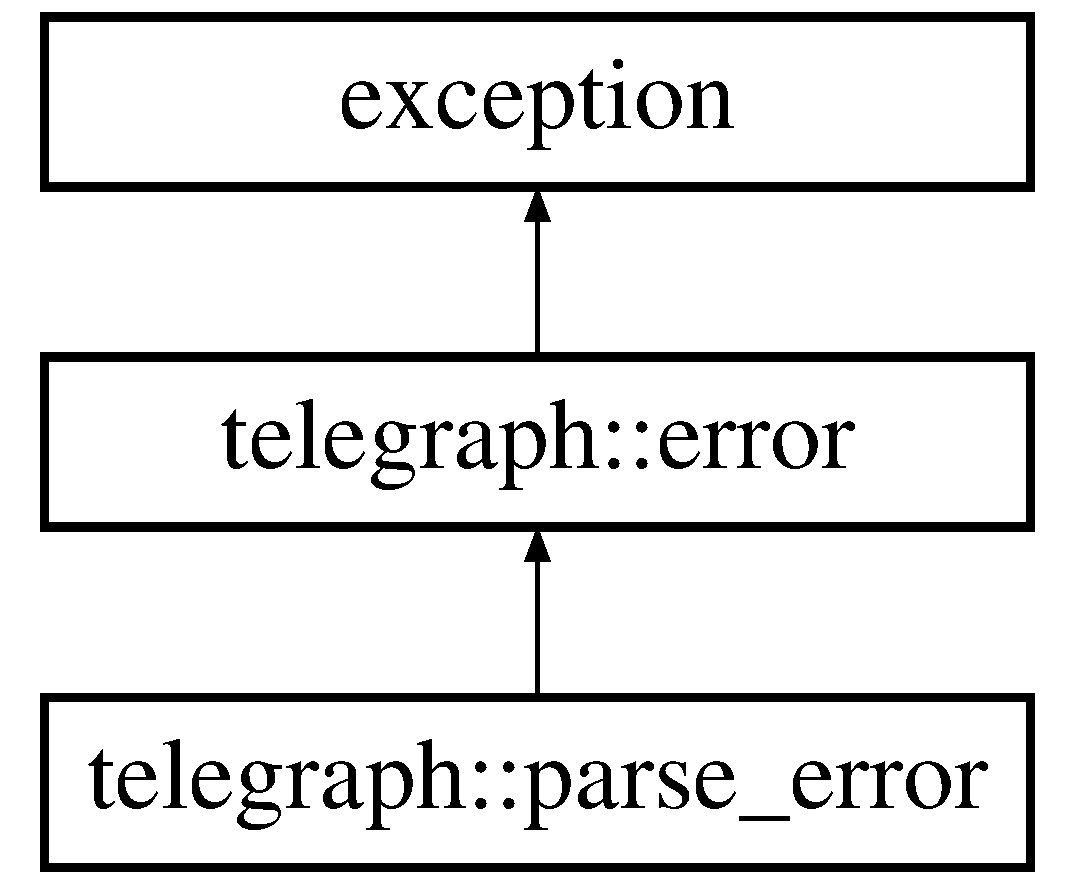
\includegraphics[height=3.000000cm]{classtelegraph_1_1parse__error}
\end{center}
\end{figure}
\subsection*{Public Member Functions}
\begin{DoxyCompactItemize}
\item 
\hyperlink{classtelegraph_1_1parse__error_afe18fb7981f6e5a6670709e07d396913}{parse\+\_\+error} (const std\+::string\+\_\+view \&m)
\end{DoxyCompactItemize}


\subsection{Constructor \& Destructor Documentation}
\mbox{\Hypertarget{classtelegraph_1_1parse__error_afe18fb7981f6e5a6670709e07d396913}\label{classtelegraph_1_1parse__error_afe18fb7981f6e5a6670709e07d396913}} 
\index{telegraph\+::parse\+\_\+error@{telegraph\+::parse\+\_\+error}!parse\+\_\+error@{parse\+\_\+error}}
\index{parse\+\_\+error@{parse\+\_\+error}!telegraph\+::parse\+\_\+error@{telegraph\+::parse\+\_\+error}}
\subsubsection{\texorpdfstring{parse\+\_\+error()}{parse\_error()}}
{\footnotesize\ttfamily telegraph\+::parse\+\_\+error\+::parse\+\_\+error (\begin{DoxyParamCaption}\item[{const std\+::string\+\_\+view \&}]{m }\end{DoxyParamCaption})\hspace{0.3cm}{\ttfamily [inline]}}



The documentation for this class was generated from the following file\+:\begin{DoxyCompactItemize}
\item 
\hyperlink{errors_8hpp}{errors.\+hpp}\end{DoxyCompactItemize}

\hypertarget{classtelegraph_1_1profile}{}\section{telegraph\+:\+:profile Class Reference}
\label{classtelegraph_1_1profile}\index{telegraph\+::profile@{telegraph\+::profile}}


{\ttfamily \#include $<$config.\+hpp$>$}

\subsection*{Public Member Functions}
\begin{DoxyCompactItemize}
\item 
\hyperlink{classtelegraph_1_1profile_a1c7b4b5e358b6210ad30410e65d921c4}{profile} (const std\+::string \&name)
\item 
\hyperlink{classtelegraph_1_1profile_adfe111d01fccdfad856ff27abf5c9959}{profile} (std\+::string \&\&name)
\item 
constexpr const std\+::string \& \hyperlink{classtelegraph_1_1profile_a93aee808f8bcec2ed60d2ab62a4a8249}{get\+\_\+name} () const
\item 
std\+::unordered\+\_\+set$<$ std\+::string $>$ \hyperlink{classtelegraph_1_1profile_aca410ddfb17eb8905541d28f668c4b9d}{sets} () const
\item 
std\+::unordered\+\_\+set$<$ \hyperlink{classtelegraph_1_1node}{node} $\ast$ $>$ \& \hyperlink{classtelegraph_1_1profile_ae55ca8f3458bc9a7b29b94320e11a075}{get} (const std\+::string \&name)
\item 
const std\+::unordered\+\_\+set$<$ \hyperlink{classtelegraph_1_1node}{node} $\ast$ $>$ \& \hyperlink{classtelegraph_1_1profile_ae815f4b8ed9bbde85fbccc48b730fadd}{get} (const std\+::string \&name) const
\item 
void \hyperlink{classtelegraph_1_1profile_ad3b7efc2c78486ded407d9f7d77c63ad}{add} (const std\+::string \&name, const std\+::unordered\+\_\+set$<$ \hyperlink{classtelegraph_1_1node}{node} $\ast$$>$ \&nodes)
\item 
void \hyperlink{classtelegraph_1_1profile_a8855f4f0091aae625de7c5eae4f548bf}{add} (const std\+::string \&name, std\+::unordered\+\_\+set$<$ \hyperlink{classtelegraph_1_1node}{node} $\ast$$>$ \&\&nodes)
\end{DoxyCompactItemize}


\subsection{Constructor \& Destructor Documentation}
\mbox{\Hypertarget{classtelegraph_1_1profile_a1c7b4b5e358b6210ad30410e65d921c4}\label{classtelegraph_1_1profile_a1c7b4b5e358b6210ad30410e65d921c4}} 
\index{telegraph\+::profile@{telegraph\+::profile}!profile@{profile}}
\index{profile@{profile}!telegraph\+::profile@{telegraph\+::profile}}
\subsubsection{\texorpdfstring{profile()}{profile()}\hspace{0.1cm}{\footnotesize\ttfamily [1/2]}}
{\footnotesize\ttfamily telegraph\+::profile\+::profile (\begin{DoxyParamCaption}\item[{const std\+::string \&}]{name }\end{DoxyParamCaption})\hspace{0.3cm}{\ttfamily [inline]}}

\mbox{\Hypertarget{classtelegraph_1_1profile_adfe111d01fccdfad856ff27abf5c9959}\label{classtelegraph_1_1profile_adfe111d01fccdfad856ff27abf5c9959}} 
\index{telegraph\+::profile@{telegraph\+::profile}!profile@{profile}}
\index{profile@{profile}!telegraph\+::profile@{telegraph\+::profile}}
\subsubsection{\texorpdfstring{profile()}{profile()}\hspace{0.1cm}{\footnotesize\ttfamily [2/2]}}
{\footnotesize\ttfamily telegraph\+::profile\+::profile (\begin{DoxyParamCaption}\item[{std\+::string \&\&}]{name }\end{DoxyParamCaption})\hspace{0.3cm}{\ttfamily [inline]}}



\subsection{Member Function Documentation}
\mbox{\Hypertarget{classtelegraph_1_1profile_ad3b7efc2c78486ded407d9f7d77c63ad}\label{classtelegraph_1_1profile_ad3b7efc2c78486ded407d9f7d77c63ad}} 
\index{telegraph\+::profile@{telegraph\+::profile}!add@{add}}
\index{add@{add}!telegraph\+::profile@{telegraph\+::profile}}
\subsubsection{\texorpdfstring{add()}{add()}\hspace{0.1cm}{\footnotesize\ttfamily [1/2]}}
{\footnotesize\ttfamily void telegraph\+::profile\+::add (\begin{DoxyParamCaption}\item[{const std\+::string \&}]{name,  }\item[{const std\+::unordered\+\_\+set$<$ \hyperlink{classtelegraph_1_1node}{node} $\ast$$>$ \&}]{nodes }\end{DoxyParamCaption})\hspace{0.3cm}{\ttfamily [inline]}}

\mbox{\Hypertarget{classtelegraph_1_1profile_a8855f4f0091aae625de7c5eae4f548bf}\label{classtelegraph_1_1profile_a8855f4f0091aae625de7c5eae4f548bf}} 
\index{telegraph\+::profile@{telegraph\+::profile}!add@{add}}
\index{add@{add}!telegraph\+::profile@{telegraph\+::profile}}
\subsubsection{\texorpdfstring{add()}{add()}\hspace{0.1cm}{\footnotesize\ttfamily [2/2]}}
{\footnotesize\ttfamily void telegraph\+::profile\+::add (\begin{DoxyParamCaption}\item[{const std\+::string \&}]{name,  }\item[{std\+::unordered\+\_\+set$<$ \hyperlink{classtelegraph_1_1node}{node} $\ast$$>$ \&\&}]{nodes }\end{DoxyParamCaption})\hspace{0.3cm}{\ttfamily [inline]}}

\mbox{\Hypertarget{classtelegraph_1_1profile_ae55ca8f3458bc9a7b29b94320e11a075}\label{classtelegraph_1_1profile_ae55ca8f3458bc9a7b29b94320e11a075}} 
\index{telegraph\+::profile@{telegraph\+::profile}!get@{get}}
\index{get@{get}!telegraph\+::profile@{telegraph\+::profile}}
\subsubsection{\texorpdfstring{get()}{get()}\hspace{0.1cm}{\footnotesize\ttfamily [1/2]}}
{\footnotesize\ttfamily std\+::unordered\+\_\+set$<$\hyperlink{classtelegraph_1_1node}{node}$\ast$$>$\& telegraph\+::profile\+::get (\begin{DoxyParamCaption}\item[{const std\+::string \&}]{name }\end{DoxyParamCaption})\hspace{0.3cm}{\ttfamily [inline]}}

\mbox{\Hypertarget{classtelegraph_1_1profile_ae815f4b8ed9bbde85fbccc48b730fadd}\label{classtelegraph_1_1profile_ae815f4b8ed9bbde85fbccc48b730fadd}} 
\index{telegraph\+::profile@{telegraph\+::profile}!get@{get}}
\index{get@{get}!telegraph\+::profile@{telegraph\+::profile}}
\subsubsection{\texorpdfstring{get()}{get()}\hspace{0.1cm}{\footnotesize\ttfamily [2/2]}}
{\footnotesize\ttfamily const std\+::unordered\+\_\+set$<$\hyperlink{classtelegraph_1_1node}{node}$\ast$$>$\& telegraph\+::profile\+::get (\begin{DoxyParamCaption}\item[{const std\+::string \&}]{name }\end{DoxyParamCaption}) const\hspace{0.3cm}{\ttfamily [inline]}}

\mbox{\Hypertarget{classtelegraph_1_1profile_a93aee808f8bcec2ed60d2ab62a4a8249}\label{classtelegraph_1_1profile_a93aee808f8bcec2ed60d2ab62a4a8249}} 
\index{telegraph\+::profile@{telegraph\+::profile}!get\+\_\+name@{get\+\_\+name}}
\index{get\+\_\+name@{get\+\_\+name}!telegraph\+::profile@{telegraph\+::profile}}
\subsubsection{\texorpdfstring{get\+\_\+name()}{get\_name()}}
{\footnotesize\ttfamily constexpr const std\+::string\& telegraph\+::profile\+::get\+\_\+name (\begin{DoxyParamCaption}{ }\end{DoxyParamCaption}) const\hspace{0.3cm}{\ttfamily [inline]}}

\mbox{\Hypertarget{classtelegraph_1_1profile_aca410ddfb17eb8905541d28f668c4b9d}\label{classtelegraph_1_1profile_aca410ddfb17eb8905541d28f668c4b9d}} 
\index{telegraph\+::profile@{telegraph\+::profile}!sets@{sets}}
\index{sets@{sets}!telegraph\+::profile@{telegraph\+::profile}}
\subsubsection{\texorpdfstring{sets()}{sets()}}
{\footnotesize\ttfamily std\+::unordered\+\_\+set$<$std\+::string$>$ telegraph\+::profile\+::sets (\begin{DoxyParamCaption}{ }\end{DoxyParamCaption}) const\hspace{0.3cm}{\ttfamily [inline]}}



The documentation for this class was generated from the following file\+:\begin{DoxyCompactItemize}
\item 
\hyperlink{config_8hpp}{config.\+hpp}\end{DoxyCompactItemize}

\hypertarget{classtelegen_1_1publisher}{}\section{telegen\+:\+:publisher$<$ T, Clock $>$ Class Template Reference}
\label{classtelegen_1_1publisher}\index{telegen\+::publisher$<$ T, Clock $>$@{telegen\+::publisher$<$ T, Clock $>$}}


{\ttfamily \#include $<$publisher.\+hpp$>$}

Inheritance diagram for telegen\+:\+:publisher$<$ T, Clock $>$\+:\begin{figure}[H]
\begin{center}
\leavevmode
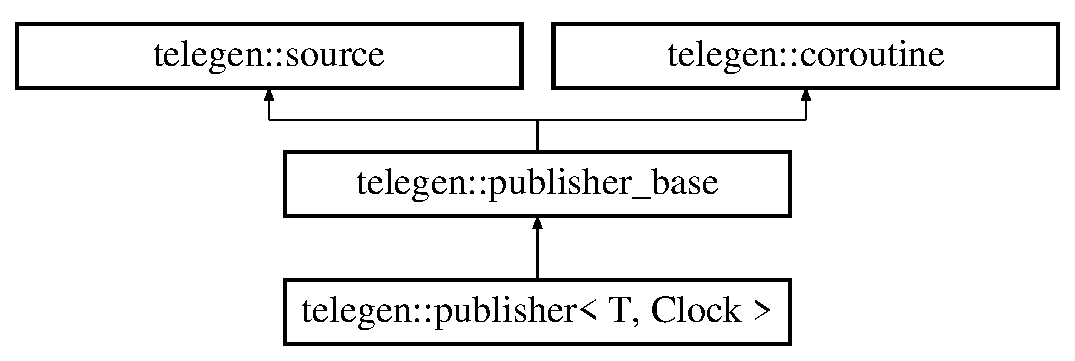
\includegraphics[height=3.000000cm]{classtelegen_1_1publisher}
\end{center}
\end{figure}
\subsection*{Classes}
\begin{DoxyCompactItemize}
\item 
class \hyperlink{classtelegen_1_1publisher_1_1sub__impl}{sub\+\_\+impl}
\end{DoxyCompactItemize}
\subsection*{Public Member Functions}
\begin{DoxyCompactItemize}
\item 
\hyperlink{classtelegen_1_1publisher_a6fc6fb74fe2e1db1de31a9ef434a851f}{publisher} (Clock $\ast$c)
\item 
\hyperlink{classtelegen_1_1publisher_adc45d3b53b7532c8b0d76673ed32f4f3}{publisher} (Clock $\ast$c, \hyperlink{classtelegen_1_1variable}{variable}$<$ T $>$ $\ast$var)
\item 
\hyperlink{classtelegen_1_1publisher_a075945686aca7ef00a37783cc5079caf}{$\sim$publisher} ()
\item 
\hyperlink{classtelegen_1_1publisher_a8b7695fbea0b0ebb4e850eb1cc1a9fd5}{publisher} (const \hyperlink{classtelegen_1_1publisher}{publisher}$<$ T, Clock $>$ \&p)=delete
\item 
void \hyperlink{classtelegen_1_1publisher_ad2111d40973f4bfd5d4bde64d736eb84}{operator=} (const \hyperlink{classtelegen_1_1publisher}{publisher}$<$ T, Clock $>$ \&p)=delete
\item 
void \hyperlink{classtelegen_1_1publisher_a3388c9262a15195d55f224bdd0606e96}{use\+\_\+for} (\hyperlink{classtelegen_1_1variable}{variable}$<$ T $>$ $\ast$var)
\item 
void \hyperlink{classtelegen_1_1publisher_a093ed11e3e992e0980dada475b154e86}{operator$<$$<$} (const T \&v)
\item 
void \hyperlink{classtelegen_1_1publisher_a551b3f77b7ac7be7157cd7cf78cc2983}{set\+\_\+alarm} (uint32\+\_\+t alarm)
\item 
void \hyperlink{classtelegen_1_1publisher_af83e62cfa8e9bbd0b43716ce7d802547}{recalculate\+\_\+next} ()
\item 
void \hyperlink{classtelegen_1_1publisher_a143382f6ff9560be4839c50b3f1dc86c}{resume} () override
\item 
\hyperlink{namespacetelegen_a9dd802bb5d30cf96b0c616750d43ae86}{promise}$<$ \hyperlink{namespacetelegen_a27c822534a5231fe1c523c81e8768afb}{subscription\+\_\+ptr} $>$ \hyperlink{classtelegen_1_1publisher_abb9ec30f9b0859e34111dc02fe8b52bd}{subscribe} (\hyperlink{classtelegen_1_1variable__base}{variable\+\_\+base} $\ast$v, \hyperlink{namespacetelegen_ad925de2d0a99bc43918533abf0457344}{interval} min\+\_\+interval, \hyperlink{namespacetelegen_ad925de2d0a99bc43918533abf0457344}{interval} max\+\_\+interval, \hyperlink{namespacetelegen_ad925de2d0a99bc43918533abf0457344}{interval} timeout) override
\item 
\hyperlink{namespacetelegen_a9dd802bb5d30cf96b0c616750d43ae86}{promise}$<$ \hyperlink{classtelegen_1_1value}{value} $>$ \hyperlink{classtelegen_1_1publisher_a3b5f514d064a6bca0209753dd724a2a7}{call} (\hyperlink{classtelegen_1_1action__base}{action\+\_\+base} $\ast$a, \hyperlink{classtelegen_1_1value}{value} arg, \hyperlink{namespacetelegen_ad925de2d0a99bc43918533abf0457344}{interval} timeout) override
\end{DoxyCompactItemize}
\subsection*{Friends}
\begin{DoxyCompactItemize}
\item 
class \hyperlink{classtelegen_1_1publisher_a378ff3f48e0298988ffbb9d03c4f5ac9}{sub\+\_\+impl}
\end{DoxyCompactItemize}


\subsection{Constructor \& Destructor Documentation}
\mbox{\Hypertarget{classtelegen_1_1publisher_a6fc6fb74fe2e1db1de31a9ef434a851f}\label{classtelegen_1_1publisher_a6fc6fb74fe2e1db1de31a9ef434a851f}} 
\index{telegen\+::publisher@{telegen\+::publisher}!publisher@{publisher}}
\index{publisher@{publisher}!telegen\+::publisher@{telegen\+::publisher}}
\subsubsection{\texorpdfstring{publisher()}{publisher()}\hspace{0.1cm}{\footnotesize\ttfamily [1/3]}}
{\footnotesize\ttfamily template$<$typename T, typename Clock$>$ \\
\hyperlink{classtelegen_1_1publisher}{telegen\+::publisher}$<$ T, Clock $>$\+::\hyperlink{classtelegen_1_1publisher}{publisher} (\begin{DoxyParamCaption}\item[{Clock $\ast$}]{c }\end{DoxyParamCaption})\hspace{0.3cm}{\ttfamily [inline]}}

\mbox{\Hypertarget{classtelegen_1_1publisher_adc45d3b53b7532c8b0d76673ed32f4f3}\label{classtelegen_1_1publisher_adc45d3b53b7532c8b0d76673ed32f4f3}} 
\index{telegen\+::publisher@{telegen\+::publisher}!publisher@{publisher}}
\index{publisher@{publisher}!telegen\+::publisher@{telegen\+::publisher}}
\subsubsection{\texorpdfstring{publisher()}{publisher()}\hspace{0.1cm}{\footnotesize\ttfamily [2/3]}}
{\footnotesize\ttfamily template$<$typename T, typename Clock$>$ \\
\hyperlink{classtelegen_1_1publisher}{telegen\+::publisher}$<$ T, Clock $>$\+::\hyperlink{classtelegen_1_1publisher}{publisher} (\begin{DoxyParamCaption}\item[{Clock $\ast$}]{c,  }\item[{\hyperlink{classtelegen_1_1variable}{variable}$<$ T $>$ $\ast$}]{var }\end{DoxyParamCaption})\hspace{0.3cm}{\ttfamily [inline]}}

\mbox{\Hypertarget{classtelegen_1_1publisher_a075945686aca7ef00a37783cc5079caf}\label{classtelegen_1_1publisher_a075945686aca7ef00a37783cc5079caf}} 
\index{telegen\+::publisher@{telegen\+::publisher}!````~publisher@{$\sim$publisher}}
\index{````~publisher@{$\sim$publisher}!telegen\+::publisher@{telegen\+::publisher}}
\subsubsection{\texorpdfstring{$\sim$publisher()}{~publisher()}}
{\footnotesize\ttfamily template$<$typename T, typename Clock$>$ \\
\hyperlink{classtelegen_1_1publisher}{telegen\+::publisher}$<$ T, Clock $>$\+::$\sim$\hyperlink{classtelegen_1_1publisher}{publisher} (\begin{DoxyParamCaption}{ }\end{DoxyParamCaption})\hspace{0.3cm}{\ttfamily [inline]}}

\mbox{\Hypertarget{classtelegen_1_1publisher_a8b7695fbea0b0ebb4e850eb1cc1a9fd5}\label{classtelegen_1_1publisher_a8b7695fbea0b0ebb4e850eb1cc1a9fd5}} 
\index{telegen\+::publisher@{telegen\+::publisher}!publisher@{publisher}}
\index{publisher@{publisher}!telegen\+::publisher@{telegen\+::publisher}}
\subsubsection{\texorpdfstring{publisher()}{publisher()}\hspace{0.1cm}{\footnotesize\ttfamily [3/3]}}
{\footnotesize\ttfamily template$<$typename T, typename Clock$>$ \\
\hyperlink{classtelegen_1_1publisher}{telegen\+::publisher}$<$ T, Clock $>$\+::\hyperlink{classtelegen_1_1publisher}{publisher} (\begin{DoxyParamCaption}\item[{const \hyperlink{classtelegen_1_1publisher}{publisher}$<$ T, Clock $>$ \&}]{p }\end{DoxyParamCaption})\hspace{0.3cm}{\ttfamily [delete]}}



\subsection{Member Function Documentation}
\mbox{\Hypertarget{classtelegen_1_1publisher_a3b5f514d064a6bca0209753dd724a2a7}\label{classtelegen_1_1publisher_a3b5f514d064a6bca0209753dd724a2a7}} 
\index{telegen\+::publisher@{telegen\+::publisher}!call@{call}}
\index{call@{call}!telegen\+::publisher@{telegen\+::publisher}}
\subsubsection{\texorpdfstring{call()}{call()}}
{\footnotesize\ttfamily template$<$typename T, typename Clock$>$ \\
\hyperlink{namespacetelegen_a9dd802bb5d30cf96b0c616750d43ae86}{promise}$<$\hyperlink{classtelegen_1_1value}{value}$>$ \hyperlink{classtelegen_1_1publisher}{telegen\+::publisher}$<$ T, Clock $>$\+::call (\begin{DoxyParamCaption}\item[{\hyperlink{classtelegen_1_1action__base}{action\+\_\+base} $\ast$}]{a,  }\item[{\hyperlink{classtelegen_1_1value}{value}}]{arg,  }\item[{\hyperlink{namespacetelegen_ad925de2d0a99bc43918533abf0457344}{interval}}]{timeout }\end{DoxyParamCaption})\hspace{0.3cm}{\ttfamily [inline]}, {\ttfamily [override]}, {\ttfamily [virtual]}}



Implements \hyperlink{classtelegen_1_1source_ae14191b0e6aa10521bb3d8fa5e1747e9}{telegen\+::source}.

\mbox{\Hypertarget{classtelegen_1_1publisher_a093ed11e3e992e0980dada475b154e86}\label{classtelegen_1_1publisher_a093ed11e3e992e0980dada475b154e86}} 
\index{telegen\+::publisher@{telegen\+::publisher}!operator$<$$<$@{operator$<$$<$}}
\index{operator$<$$<$@{operator$<$$<$}!telegen\+::publisher@{telegen\+::publisher}}
\subsubsection{\texorpdfstring{operator$<$$<$()}{operator<<()}}
{\footnotesize\ttfamily template$<$typename T, typename Clock$>$ \\
void \hyperlink{classtelegen_1_1publisher}{telegen\+::publisher}$<$ T, Clock $>$\+::operator$<$$<$ (\begin{DoxyParamCaption}\item[{const T \&}]{v }\end{DoxyParamCaption})\hspace{0.3cm}{\ttfamily [inline]}}

\mbox{\Hypertarget{classtelegen_1_1publisher_ad2111d40973f4bfd5d4bde64d736eb84}\label{classtelegen_1_1publisher_ad2111d40973f4bfd5d4bde64d736eb84}} 
\index{telegen\+::publisher@{telegen\+::publisher}!operator=@{operator=}}
\index{operator=@{operator=}!telegen\+::publisher@{telegen\+::publisher}}
\subsubsection{\texorpdfstring{operator=()}{operator=()}}
{\footnotesize\ttfamily template$<$typename T, typename Clock$>$ \\
void \hyperlink{classtelegen_1_1publisher}{telegen\+::publisher}$<$ T, Clock $>$\+::operator= (\begin{DoxyParamCaption}\item[{const \hyperlink{classtelegen_1_1publisher}{publisher}$<$ T, Clock $>$ \&}]{p }\end{DoxyParamCaption})\hspace{0.3cm}{\ttfamily [delete]}}

\mbox{\Hypertarget{classtelegen_1_1publisher_af83e62cfa8e9bbd0b43716ce7d802547}\label{classtelegen_1_1publisher_af83e62cfa8e9bbd0b43716ce7d802547}} 
\index{telegen\+::publisher@{telegen\+::publisher}!recalculate\+\_\+next@{recalculate\+\_\+next}}
\index{recalculate\+\_\+next@{recalculate\+\_\+next}!telegen\+::publisher@{telegen\+::publisher}}
\subsubsection{\texorpdfstring{recalculate\+\_\+next()}{recalculate\_next()}}
{\footnotesize\ttfamily template$<$typename T, typename Clock$>$ \\
void \hyperlink{classtelegen_1_1publisher}{telegen\+::publisher}$<$ T, Clock $>$\+::recalculate\+\_\+next (\begin{DoxyParamCaption}{ }\end{DoxyParamCaption})\hspace{0.3cm}{\ttfamily [inline]}}

\mbox{\Hypertarget{classtelegen_1_1publisher_a143382f6ff9560be4839c50b3f1dc86c}\label{classtelegen_1_1publisher_a143382f6ff9560be4839c50b3f1dc86c}} 
\index{telegen\+::publisher@{telegen\+::publisher}!resume@{resume}}
\index{resume@{resume}!telegen\+::publisher@{telegen\+::publisher}}
\subsubsection{\texorpdfstring{resume()}{resume()}}
{\footnotesize\ttfamily template$<$typename T, typename Clock$>$ \\
void \hyperlink{classtelegen_1_1publisher}{telegen\+::publisher}$<$ T, Clock $>$\+::resume (\begin{DoxyParamCaption}{ }\end{DoxyParamCaption})\hspace{0.3cm}{\ttfamily [inline]}, {\ttfamily [override]}, {\ttfamily [virtual]}}



Implements \hyperlink{structtelegen_1_1coroutine_a2a7408a5b9474af3e59128934e3a5c00}{telegen\+::coroutine}.

\mbox{\Hypertarget{classtelegen_1_1publisher_a551b3f77b7ac7be7157cd7cf78cc2983}\label{classtelegen_1_1publisher_a551b3f77b7ac7be7157cd7cf78cc2983}} 
\index{telegen\+::publisher@{telegen\+::publisher}!set\+\_\+alarm@{set\+\_\+alarm}}
\index{set\+\_\+alarm@{set\+\_\+alarm}!telegen\+::publisher@{telegen\+::publisher}}
\subsubsection{\texorpdfstring{set\+\_\+alarm()}{set\_alarm()}}
{\footnotesize\ttfamily template$<$typename T, typename Clock$>$ \\
void \hyperlink{classtelegen_1_1publisher}{telegen\+::publisher}$<$ T, Clock $>$\+::set\+\_\+alarm (\begin{DoxyParamCaption}\item[{uint32\+\_\+t}]{alarm }\end{DoxyParamCaption})\hspace{0.3cm}{\ttfamily [inline]}}

\mbox{\Hypertarget{classtelegen_1_1publisher_abb9ec30f9b0859e34111dc02fe8b52bd}\label{classtelegen_1_1publisher_abb9ec30f9b0859e34111dc02fe8b52bd}} 
\index{telegen\+::publisher@{telegen\+::publisher}!subscribe@{subscribe}}
\index{subscribe@{subscribe}!telegen\+::publisher@{telegen\+::publisher}}
\subsubsection{\texorpdfstring{subscribe()}{subscribe()}}
{\footnotesize\ttfamily template$<$typename T, typename Clock$>$ \\
\hyperlink{namespacetelegen_a9dd802bb5d30cf96b0c616750d43ae86}{promise}$<$\hyperlink{namespacetelegen_a27c822534a5231fe1c523c81e8768afb}{subscription\+\_\+ptr}$>$ \hyperlink{classtelegen_1_1publisher}{telegen\+::publisher}$<$ T, Clock $>$\+::subscribe (\begin{DoxyParamCaption}\item[{\hyperlink{classtelegen_1_1variable__base}{variable\+\_\+base} $\ast$}]{v,  }\item[{\hyperlink{namespacetelegen_ad925de2d0a99bc43918533abf0457344}{interval}}]{min\+\_\+interval,  }\item[{\hyperlink{namespacetelegen_ad925de2d0a99bc43918533abf0457344}{interval}}]{max\+\_\+interval,  }\item[{\hyperlink{namespacetelegen_ad925de2d0a99bc43918533abf0457344}{interval}}]{timeout }\end{DoxyParamCaption})\hspace{0.3cm}{\ttfamily [inline]}, {\ttfamily [override]}, {\ttfamily [virtual]}}



Implements \hyperlink{classtelegen_1_1source_a224b4eb02ea346aca099615a5ae00ea9}{telegen\+::source}.

\mbox{\Hypertarget{classtelegen_1_1publisher_a3388c9262a15195d55f224bdd0606e96}\label{classtelegen_1_1publisher_a3388c9262a15195d55f224bdd0606e96}} 
\index{telegen\+::publisher@{telegen\+::publisher}!use\+\_\+for@{use\+\_\+for}}
\index{use\+\_\+for@{use\+\_\+for}!telegen\+::publisher@{telegen\+::publisher}}
\subsubsection{\texorpdfstring{use\+\_\+for()}{use\_for()}}
{\footnotesize\ttfamily template$<$typename T, typename Clock$>$ \\
void \hyperlink{classtelegen_1_1publisher}{telegen\+::publisher}$<$ T, Clock $>$\+::use\+\_\+for (\begin{DoxyParamCaption}\item[{\hyperlink{classtelegen_1_1variable}{variable}$<$ T $>$ $\ast$}]{var }\end{DoxyParamCaption})\hspace{0.3cm}{\ttfamily [inline]}}



\subsection{Friends And Related Function Documentation}
\mbox{\Hypertarget{classtelegen_1_1publisher_a378ff3f48e0298988ffbb9d03c4f5ac9}\label{classtelegen_1_1publisher_a378ff3f48e0298988ffbb9d03c4f5ac9}} 
\index{telegen\+::publisher@{telegen\+::publisher}!sub\+\_\+impl@{sub\+\_\+impl}}
\index{sub\+\_\+impl@{sub\+\_\+impl}!telegen\+::publisher@{telegen\+::publisher}}
\subsubsection{\texorpdfstring{sub\+\_\+impl}{sub\_impl}}
{\footnotesize\ttfamily template$<$typename T, typename Clock$>$ \\
friend class \hyperlink{classtelegen_1_1publisher_1_1sub__impl}{sub\+\_\+impl}\hspace{0.3cm}{\ttfamily [friend]}}



The documentation for this class was generated from the following file\+:\begin{DoxyCompactItemize}
\item 
\hyperlink{gen_2telegen_2publisher_8hpp}{gen/telegen/publisher.\+hpp}\end{DoxyCompactItemize}

\hypertarget{classtelegraph_1_1publisher}{}\section{telegraph\+:\+:publisher Class Reference}
\label{classtelegraph_1_1publisher}\index{telegraph\+::publisher@{telegraph\+::publisher}}


{\ttfamily \#include $<$publisher.\+hpp$>$}

Inheritance diagram for telegraph\+:\+:publisher\+:\begin{figure}[H]
\begin{center}
\leavevmode
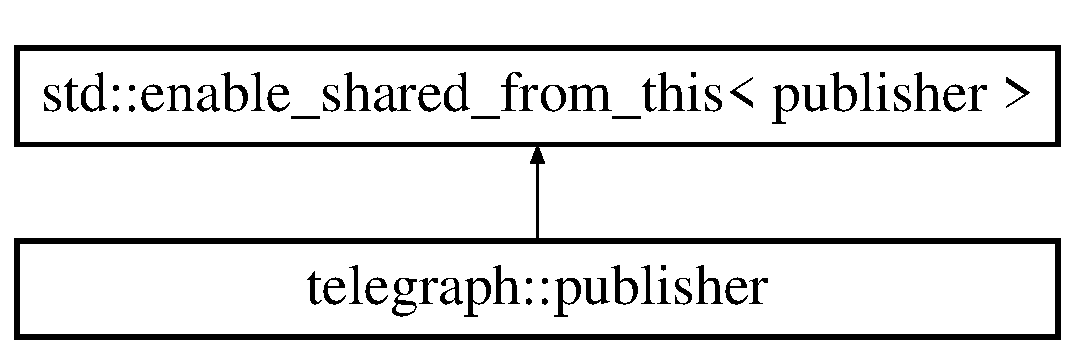
\includegraphics[height=2.000000cm]{classtelegraph_1_1publisher}
\end{center}
\end{figure}
\subsection*{Public Member Functions}
\begin{DoxyCompactItemize}
\item 
\hyperlink{classtelegraph_1_1publisher_a8ae019593c70465dc12354a08c26efed}{publisher} (io\+::io\+\_\+context \&ioc, \hyperlink{classtelegraph_1_1value__type}{value\+\_\+type} t)
\item 
\hyperlink{classtelegraph_1_1publisher_a69bd0368a3a03a2a26c45768cabaaea6}{$\sim$publisher} ()
\item 
\hyperlink{namespacetelegraph_a58641aa5b1a2cbdb0431916a87069f64}{subscription\+\_\+ptr} \hyperlink{classtelegraph_1_1publisher_a9ecf7dc2e9366618be852b04485a00eb}{subscribe} (float min\+\_\+interval, float max\+\_\+interval)
\item 
void \hyperlink{classtelegraph_1_1publisher_afe6033c401deb3af2a849e5059def250}{update} (\hyperlink{classtelegraph_1_1value}{value} v)
\item 
\hyperlink{classtelegraph_1_1publisher}{publisher} \& \hyperlink{classtelegraph_1_1publisher_a48b08a6577fd2b047186217adbfa5b83}{operator$<$$<$} (\hyperlink{classtelegraph_1_1value}{value} v)
\end{DoxyCompactItemize}


\subsection{Constructor \& Destructor Documentation}
\mbox{\Hypertarget{classtelegraph_1_1publisher_a8ae019593c70465dc12354a08c26efed}\label{classtelegraph_1_1publisher_a8ae019593c70465dc12354a08c26efed}} 
\index{telegraph\+::publisher@{telegraph\+::publisher}!publisher@{publisher}}
\index{publisher@{publisher}!telegraph\+::publisher@{telegraph\+::publisher}}
\subsubsection{\texorpdfstring{publisher()}{publisher()}}
{\footnotesize\ttfamily telegraph\+::publisher\+::publisher (\begin{DoxyParamCaption}\item[{io\+::io\+\_\+context \&}]{ioc,  }\item[{\hyperlink{classtelegraph_1_1value__type}{value\+\_\+type}}]{t }\end{DoxyParamCaption})\hspace{0.3cm}{\ttfamily [inline]}}

\mbox{\Hypertarget{classtelegraph_1_1publisher_a69bd0368a3a03a2a26c45768cabaaea6}\label{classtelegraph_1_1publisher_a69bd0368a3a03a2a26c45768cabaaea6}} 
\index{telegraph\+::publisher@{telegraph\+::publisher}!````~publisher@{$\sim$publisher}}
\index{````~publisher@{$\sim$publisher}!telegraph\+::publisher@{telegraph\+::publisher}}
\subsubsection{\texorpdfstring{$\sim$publisher()}{~publisher()}}
{\footnotesize\ttfamily telegraph\+::publisher\+::$\sim$publisher (\begin{DoxyParamCaption}{ }\end{DoxyParamCaption})\hspace{0.3cm}{\ttfamily [inline]}}



\subsection{Member Function Documentation}
\mbox{\Hypertarget{classtelegraph_1_1publisher_a48b08a6577fd2b047186217adbfa5b83}\label{classtelegraph_1_1publisher_a48b08a6577fd2b047186217adbfa5b83}} 
\index{telegraph\+::publisher@{telegraph\+::publisher}!operator$<$$<$@{operator$<$$<$}}
\index{operator$<$$<$@{operator$<$$<$}!telegraph\+::publisher@{telegraph\+::publisher}}
\subsubsection{\texorpdfstring{operator$<$$<$()}{operator<<()}}
{\footnotesize\ttfamily \hyperlink{classtelegraph_1_1publisher}{publisher}\& telegraph\+::publisher\+::operator$<$$<$ (\begin{DoxyParamCaption}\item[{\hyperlink{classtelegraph_1_1value}{value}}]{v }\end{DoxyParamCaption})\hspace{0.3cm}{\ttfamily [inline]}}

\mbox{\Hypertarget{classtelegraph_1_1publisher_a9ecf7dc2e9366618be852b04485a00eb}\label{classtelegraph_1_1publisher_a9ecf7dc2e9366618be852b04485a00eb}} 
\index{telegraph\+::publisher@{telegraph\+::publisher}!subscribe@{subscribe}}
\index{subscribe@{subscribe}!telegraph\+::publisher@{telegraph\+::publisher}}
\subsubsection{\texorpdfstring{subscribe()}{subscribe()}}
{\footnotesize\ttfamily \hyperlink{namespacetelegraph_a58641aa5b1a2cbdb0431916a87069f64}{subscription\+\_\+ptr} telegraph\+::publisher\+::subscribe (\begin{DoxyParamCaption}\item[{float}]{min\+\_\+interval,  }\item[{float}]{max\+\_\+interval }\end{DoxyParamCaption})\hspace{0.3cm}{\ttfamily [inline]}}

\mbox{\Hypertarget{classtelegraph_1_1publisher_afe6033c401deb3af2a849e5059def250}\label{classtelegraph_1_1publisher_afe6033c401deb3af2a849e5059def250}} 
\index{telegraph\+::publisher@{telegraph\+::publisher}!update@{update}}
\index{update@{update}!telegraph\+::publisher@{telegraph\+::publisher}}
\subsubsection{\texorpdfstring{update()}{update()}}
{\footnotesize\ttfamily void telegraph\+::publisher\+::update (\begin{DoxyParamCaption}\item[{\hyperlink{classtelegraph_1_1value}{value}}]{v }\end{DoxyParamCaption})\hspace{0.3cm}{\ttfamily [inline]}}



The documentation for this class was generated from the following file\+:\begin{DoxyCompactItemize}
\item 
\hyperlink{lib_2telegraph_2common_2publisher_8hpp}{lib/telegraph/common/publisher.\+hpp}\end{DoxyCompactItemize}

\hypertarget{classtelegen_1_1publisher__base}{}\section{telegen\+:\+:publisher\+\_\+base Class Reference}
\label{classtelegen_1_1publisher__base}\index{telegen\+::publisher\+\_\+base@{telegen\+::publisher\+\_\+base}}


{\ttfamily \#include $<$publisher.\+hpp$>$}

Inheritance diagram for telegen\+:\+:publisher\+\_\+base\+:\begin{figure}[H]
\begin{center}
\leavevmode
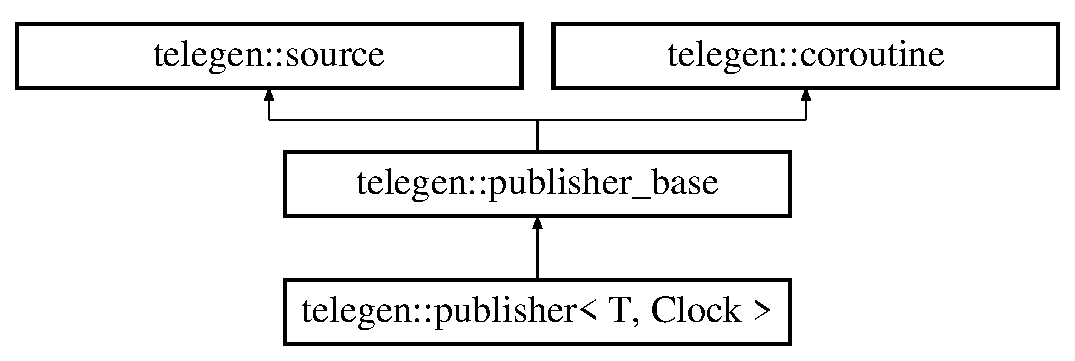
\includegraphics[height=3.000000cm]{classtelegen_1_1publisher__base}
\end{center}
\end{figure}
\subsection*{Additional Inherited Members}


The documentation for this class was generated from the following file\+:\begin{DoxyCompactItemize}
\item 
\hyperlink{gen_2telegen_2publisher_8hpp}{gen/telegen/publisher.\+hpp}\end{DoxyCompactItemize}

\hypertarget{classtelegen_1_1publisher__scheduler}{}\section{telegen\+:\+:publisher\+\_\+scheduler Class Reference}
\label{classtelegen_1_1publisher__scheduler}\index{telegen\+::publisher\+\_\+scheduler@{telegen\+::publisher\+\_\+scheduler}}


{\ttfamily \#include $<$publisher.\+hpp$>$}

Inheritance diagram for telegen\+:\+:publisher\+\_\+scheduler\+:\begin{figure}[H]
\begin{center}
\leavevmode
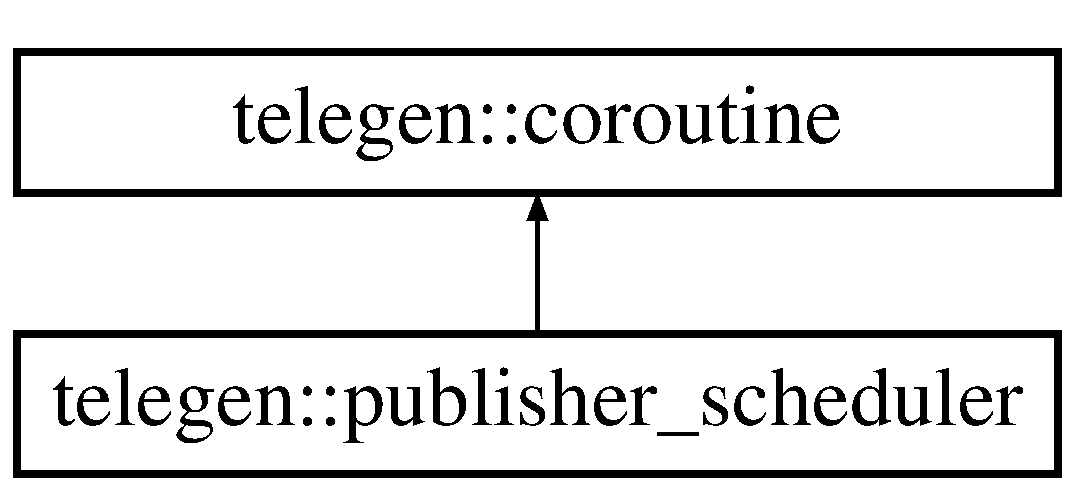
\includegraphics[height=2.000000cm]{classtelegen_1_1publisher__scheduler}
\end{center}
\end{figure}
\subsection*{Additional Inherited Members}


The documentation for this class was generated from the following file\+:\begin{DoxyCompactItemize}
\item 
\hyperlink{gen_2telegen_2publisher_8hpp}{gen/telegen/publisher.\+hpp}\end{DoxyCompactItemize}

\hypertarget{classtelegen_1_1coroutine_1_1ref}{}\section{telegen\+:\+:coroutine\+:\+:ref Class Reference}
\label{classtelegen_1_1coroutine_1_1ref}\index{telegen\+::coroutine\+::ref@{telegen\+::coroutine\+::ref}}


{\ttfamily \#include $<$coroutine.\+hpp$>$}

\subsection*{Public Member Functions}
\begin{DoxyCompactItemize}
\item 
\hyperlink{classtelegen_1_1coroutine_1_1ref_a04d38625676996ee154a2228496b4ed0}{ref} (\hyperlink{structtelegen_1_1coroutine}{coroutine} \&c)
\item 
\hyperlink{classtelegen_1_1coroutine_1_1ref_a40fa879f483f552a0de04d2047d3fb00}{ref} (\hyperlink{structtelegen_1_1coroutine}{coroutine} $\ast$c)
\item 
\hyperlink{classtelegen_1_1coroutine_1_1ref_a4e11df44835cad42e04f9eebe7096dbd}{$\sim$ref} ()
\item 
\hyperlink{classtelegen_1_1coroutine_1_1ref_a40534b7249731bd182032f2175080d2f}{operator int} () const
\item 
int \& \hyperlink{classtelegen_1_1coroutine_1_1ref_a4df06629c2ca9c502184c8e066c64213}{operator=} (int bp)
\end{DoxyCompactItemize}


\subsection{Constructor \& Destructor Documentation}
\mbox{\Hypertarget{classtelegen_1_1coroutine_1_1ref_a04d38625676996ee154a2228496b4ed0}\label{classtelegen_1_1coroutine_1_1ref_a04d38625676996ee154a2228496b4ed0}} 
\index{telegen\+::coroutine\+::ref@{telegen\+::coroutine\+::ref}!ref@{ref}}
\index{ref@{ref}!telegen\+::coroutine\+::ref@{telegen\+::coroutine\+::ref}}
\subsubsection{\texorpdfstring{ref()}{ref()}\hspace{0.1cm}{\footnotesize\ttfamily [1/2]}}
{\footnotesize\ttfamily telegen\+::coroutine\+::ref\+::ref (\begin{DoxyParamCaption}\item[{\hyperlink{structtelegen_1_1coroutine}{coroutine} \&}]{c }\end{DoxyParamCaption})\hspace{0.3cm}{\ttfamily [inline]}}

\mbox{\Hypertarget{classtelegen_1_1coroutine_1_1ref_a40fa879f483f552a0de04d2047d3fb00}\label{classtelegen_1_1coroutine_1_1ref_a40fa879f483f552a0de04d2047d3fb00}} 
\index{telegen\+::coroutine\+::ref@{telegen\+::coroutine\+::ref}!ref@{ref}}
\index{ref@{ref}!telegen\+::coroutine\+::ref@{telegen\+::coroutine\+::ref}}
\subsubsection{\texorpdfstring{ref()}{ref()}\hspace{0.1cm}{\footnotesize\ttfamily [2/2]}}
{\footnotesize\ttfamily telegen\+::coroutine\+::ref\+::ref (\begin{DoxyParamCaption}\item[{\hyperlink{structtelegen_1_1coroutine}{coroutine} $\ast$}]{c }\end{DoxyParamCaption})\hspace{0.3cm}{\ttfamily [inline]}}

\mbox{\Hypertarget{classtelegen_1_1coroutine_1_1ref_a4e11df44835cad42e04f9eebe7096dbd}\label{classtelegen_1_1coroutine_1_1ref_a4e11df44835cad42e04f9eebe7096dbd}} 
\index{telegen\+::coroutine\+::ref@{telegen\+::coroutine\+::ref}!````~ref@{$\sim$ref}}
\index{````~ref@{$\sim$ref}!telegen\+::coroutine\+::ref@{telegen\+::coroutine\+::ref}}
\subsubsection{\texorpdfstring{$\sim$ref()}{~ref()}}
{\footnotesize\ttfamily telegen\+::coroutine\+::ref\+::$\sim$ref (\begin{DoxyParamCaption}{ }\end{DoxyParamCaption})\hspace{0.3cm}{\ttfamily [inline]}}



\subsection{Member Function Documentation}
\mbox{\Hypertarget{classtelegen_1_1coroutine_1_1ref_a40534b7249731bd182032f2175080d2f}\label{classtelegen_1_1coroutine_1_1ref_a40534b7249731bd182032f2175080d2f}} 
\index{telegen\+::coroutine\+::ref@{telegen\+::coroutine\+::ref}!operator int@{operator int}}
\index{operator int@{operator int}!telegen\+::coroutine\+::ref@{telegen\+::coroutine\+::ref}}
\subsubsection{\texorpdfstring{operator int()}{operator int()}}
{\footnotesize\ttfamily telegen\+::coroutine\+::ref\+::operator int (\begin{DoxyParamCaption}{ }\end{DoxyParamCaption}) const\hspace{0.3cm}{\ttfamily [inline]}}

\mbox{\Hypertarget{classtelegen_1_1coroutine_1_1ref_a4df06629c2ca9c502184c8e066c64213}\label{classtelegen_1_1coroutine_1_1ref_a4df06629c2ca9c502184c8e066c64213}} 
\index{telegen\+::coroutine\+::ref@{telegen\+::coroutine\+::ref}!operator=@{operator=}}
\index{operator=@{operator=}!telegen\+::coroutine\+::ref@{telegen\+::coroutine\+::ref}}
\subsubsection{\texorpdfstring{operator=()}{operator=()}}
{\footnotesize\ttfamily int\& telegen\+::coroutine\+::ref\+::operator= (\begin{DoxyParamCaption}\item[{int}]{bp }\end{DoxyParamCaption})\hspace{0.3cm}{\ttfamily [inline]}}



The documentation for this class was generated from the following file\+:\begin{DoxyCompactItemize}
\item 
\hyperlink{coroutine_8hpp}{coroutine.\+hpp}\end{DoxyCompactItemize}

\hypertarget{classtelegraph_1_1server_1_1remote}{}\section{telegraph\+:\+:server\+:\+:remote Class Reference}
\label{classtelegraph_1_1server_1_1remote}\index{telegraph\+::server\+::remote@{telegraph\+::server\+::remote}}


{\ttfamily \#include $<$server.\+hpp$>$}

Inheritance diagram for telegraph\+:\+:server\+:\+:remote\+:\begin{figure}[H]
\begin{center}
\leavevmode
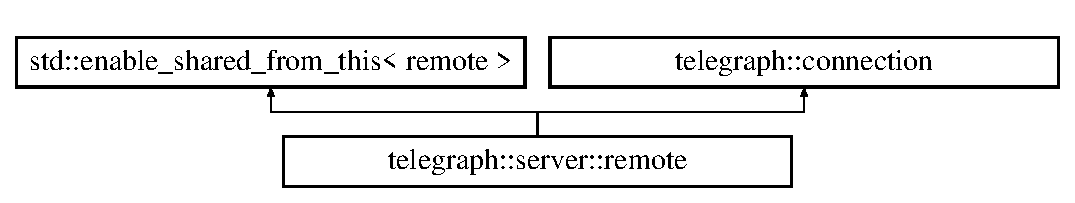
\includegraphics[height=2.000000cm]{classtelegraph_1_1server_1_1remote}
\end{center}
\end{figure}
\subsection*{Public Member Functions}
\begin{DoxyCompactItemize}
\item 
\hyperlink{classtelegraph_1_1server_1_1remote_a90eb5976be1536b518b89debfba36843}{remote} (io\+::io\+\_\+context \&ioc, boost\+::asio\+::ip\+::tcp\+::socket \&\&socket, const std\+::shared\+\_\+ptr$<$ \hyperlink{classtelegraph_1_1namespace__}{namespace\+\_\+} $>$ \&local)
\item 
void \hyperlink{classtelegraph_1_1server_1_1remote_aa6a2f2d4045ea8bb51938ca3da4e1b5e}{send} (api\+::\+Packet \&\&p) override
\item 
void \hyperlink{classtelegraph_1_1server_1_1remote_a10d60a8be9442784f3f1d63492835841}{do\+\_\+accept} ()
\end{DoxyCompactItemize}


\subsection{Constructor \& Destructor Documentation}
\mbox{\Hypertarget{classtelegraph_1_1server_1_1remote_a90eb5976be1536b518b89debfba36843}\label{classtelegraph_1_1server_1_1remote_a90eb5976be1536b518b89debfba36843}} 
\index{telegraph\+::server\+::remote@{telegraph\+::server\+::remote}!remote@{remote}}
\index{remote@{remote}!telegraph\+::server\+::remote@{telegraph\+::server\+::remote}}
\subsubsection{\texorpdfstring{remote()}{remote()}}
{\footnotesize\ttfamily telegraph\+::server\+::remote\+::remote (\begin{DoxyParamCaption}\item[{io\+::io\+\_\+context \&}]{ioc,  }\item[{boost\+::asio\+::ip\+::tcp\+::socket \&\&}]{socket,  }\item[{const std\+::shared\+\_\+ptr$<$ \hyperlink{classtelegraph_1_1namespace__}{namespace\+\_\+} $>$ \&}]{local }\end{DoxyParamCaption})}



\subsection{Member Function Documentation}
\mbox{\Hypertarget{classtelegraph_1_1server_1_1remote_a10d60a8be9442784f3f1d63492835841}\label{classtelegraph_1_1server_1_1remote_a10d60a8be9442784f3f1d63492835841}} 
\index{telegraph\+::server\+::remote@{telegraph\+::server\+::remote}!do\+\_\+accept@{do\+\_\+accept}}
\index{do\+\_\+accept@{do\+\_\+accept}!telegraph\+::server\+::remote@{telegraph\+::server\+::remote}}
\subsubsection{\texorpdfstring{do\+\_\+accept()}{do\_accept()}}
{\footnotesize\ttfamily void telegraph\+::server\+::remote\+::do\+\_\+accept (\begin{DoxyParamCaption}{ }\end{DoxyParamCaption})}

\mbox{\Hypertarget{classtelegraph_1_1server_1_1remote_aa6a2f2d4045ea8bb51938ca3da4e1b5e}\label{classtelegraph_1_1server_1_1remote_aa6a2f2d4045ea8bb51938ca3da4e1b5e}} 
\index{telegraph\+::server\+::remote@{telegraph\+::server\+::remote}!send@{send}}
\index{send@{send}!telegraph\+::server\+::remote@{telegraph\+::server\+::remote}}
\subsubsection{\texorpdfstring{send()}{send()}}
{\footnotesize\ttfamily void telegraph\+::server\+::remote\+::send (\begin{DoxyParamCaption}\item[{api\+::\+Packet \&\&}]{p }\end{DoxyParamCaption})\hspace{0.3cm}{\ttfamily [override]}, {\ttfamily [virtual]}}



Implements \hyperlink{classtelegraph_1_1connection_ad5fd2c23680ecda6e07c2f02f3735809}{telegraph\+::connection}.



The documentation for this class was generated from the following files\+:\begin{DoxyCompactItemize}
\item 
\hyperlink{server_8hpp}{server.\+hpp}\item 
\hyperlink{lib_2telegraph_2remote_2server_8cpp}{lib/telegraph/remote/server.\+cpp}\end{DoxyCompactItemize}

\hypertarget{classtelegraph_1_1remote__error}{}\section{telegraph\+:\+:remote\+\_\+error Class Reference}
\label{classtelegraph_1_1remote__error}\index{telegraph\+::remote\+\_\+error@{telegraph\+::remote\+\_\+error}}


{\ttfamily \#include $<$errors.\+hpp$>$}

Inheritance diagram for telegraph\+:\+:remote\+\_\+error\+:\begin{figure}[H]
\begin{center}
\leavevmode
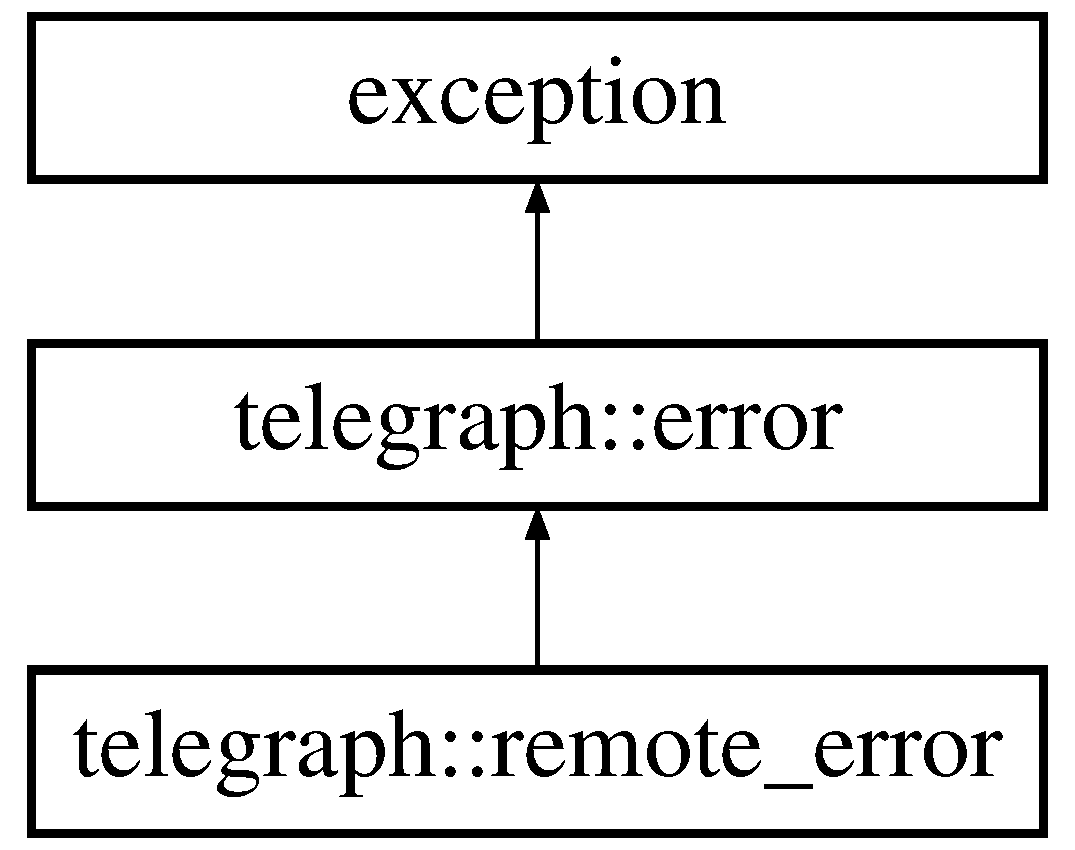
\includegraphics[height=3.000000cm]{classtelegraph_1_1remote__error}
\end{center}
\end{figure}
\subsection*{Public Member Functions}
\begin{DoxyCompactItemize}
\item 
\hyperlink{classtelegraph_1_1remote__error_a9d7461b65c248393e6cb22bd243fc5c4}{remote\+\_\+error} (const std\+::string\+\_\+view \&m)
\end{DoxyCompactItemize}


\subsection{Constructor \& Destructor Documentation}
\mbox{\Hypertarget{classtelegraph_1_1remote__error_a9d7461b65c248393e6cb22bd243fc5c4}\label{classtelegraph_1_1remote__error_a9d7461b65c248393e6cb22bd243fc5c4}} 
\index{telegraph\+::remote\+\_\+error@{telegraph\+::remote\+\_\+error}!remote\+\_\+error@{remote\+\_\+error}}
\index{remote\+\_\+error@{remote\+\_\+error}!telegraph\+::remote\+\_\+error@{telegraph\+::remote\+\_\+error}}
\subsubsection{\texorpdfstring{remote\+\_\+error()}{remote\_error()}}
{\footnotesize\ttfamily telegraph\+::remote\+\_\+error\+::remote\+\_\+error (\begin{DoxyParamCaption}\item[{const std\+::string\+\_\+view \&}]{m }\end{DoxyParamCaption})\hspace{0.3cm}{\ttfamily [inline]}}



The documentation for this class was generated from the following file\+:\begin{DoxyCompactItemize}
\item 
\hyperlink{errors_8hpp}{errors.\+hpp}\end{DoxyCompactItemize}

\hypertarget{structtelegraph_1_1generator_1_1result}{}\section{telegraph\+:\+:generator\+:\+:result Struct Reference}
\label{structtelegraph_1_1generator_1_1result}\index{telegraph\+::generator\+::result@{telegraph\+::generator\+::result}}


{\ttfamily \#include $<$generator.\+hpp$>$}

\subsection*{Public Member Functions}
\begin{DoxyCompactItemize}
\item 
\hyperlink{structtelegraph_1_1generator_1_1result_ada8a0a692c8400c494dee7c3bf887089}{result} ()
\end{DoxyCompactItemize}
\subsection*{Public Attributes}
\begin{DoxyCompactItemize}
\item 
std\+::string \hyperlink{structtelegraph_1_1generator_1_1result_a1c61e7b62edde7e2189aee9f1007b2f5}{filename}
\item 
std\+::string \hyperlink{structtelegraph_1_1generator_1_1result_a2ad8db06b54ff998dcd2b407c855eb6e}{code}
\end{DoxyCompactItemize}


\subsection{Constructor \& Destructor Documentation}
\mbox{\Hypertarget{structtelegraph_1_1generator_1_1result_ada8a0a692c8400c494dee7c3bf887089}\label{structtelegraph_1_1generator_1_1result_ada8a0a692c8400c494dee7c3bf887089}} 
\index{telegraph\+::generator\+::result@{telegraph\+::generator\+::result}!result@{result}}
\index{result@{result}!telegraph\+::generator\+::result@{telegraph\+::generator\+::result}}
\subsubsection{\texorpdfstring{result()}{result()}}
{\footnotesize\ttfamily telegraph\+::generator\+::result\+::result (\begin{DoxyParamCaption}{ }\end{DoxyParamCaption})\hspace{0.3cm}{\ttfamily [inline]}}



\subsection{Member Data Documentation}
\mbox{\Hypertarget{structtelegraph_1_1generator_1_1result_a2ad8db06b54ff998dcd2b407c855eb6e}\label{structtelegraph_1_1generator_1_1result_a2ad8db06b54ff998dcd2b407c855eb6e}} 
\index{telegraph\+::generator\+::result@{telegraph\+::generator\+::result}!code@{code}}
\index{code@{code}!telegraph\+::generator\+::result@{telegraph\+::generator\+::result}}
\subsubsection{\texorpdfstring{code}{code}}
{\footnotesize\ttfamily std\+::string telegraph\+::generator\+::result\+::code}

\mbox{\Hypertarget{structtelegraph_1_1generator_1_1result_a1c61e7b62edde7e2189aee9f1007b2f5}\label{structtelegraph_1_1generator_1_1result_a1c61e7b62edde7e2189aee9f1007b2f5}} 
\index{telegraph\+::generator\+::result@{telegraph\+::generator\+::result}!filename@{filename}}
\index{filename@{filename}!telegraph\+::generator\+::result@{telegraph\+::generator\+::result}}
\subsubsection{\texorpdfstring{filename}{filename}}
{\footnotesize\ttfamily std\+::string telegraph\+::generator\+::result\+::filename}



The documentation for this struct was generated from the following file\+:\begin{DoxyCompactItemize}
\item 
\hyperlink{generator_8hpp}{generator.\+hpp}\end{DoxyCompactItemize}

\hypertarget{classtelegraph_1_1server}{}\section{telegraph\+:\+:server Class Reference}
\label{classtelegraph_1_1server}\index{telegraph\+::server@{telegraph\+::server}}


{\ttfamily \#include $<$server.\+hpp$>$}

\subsection*{Classes}
\begin{DoxyCompactItemize}
\item 
class \hyperlink{classtelegraph_1_1server_1_1remote}{remote}
\end{DoxyCompactItemize}
\subsection*{Public Member Functions}
\begin{DoxyCompactItemize}
\item 
\hyperlink{classtelegraph_1_1server_ab1016347c0288b33aa5cf38a70928351}{server} (io\+::io\+\_\+context \&ioc, boost\+::asio\+::ip\+::tcp\+::endpoint ep, const std\+::shared\+\_\+ptr$<$ \hyperlink{classtelegraph_1_1namespace__}{namespace\+\_\+} $>$ \&local)
\item 
void \hyperlink{classtelegraph_1_1server_ad7bf15056564c266ea630e35157758bc}{run} (\hyperlink{structboost_1_1asio_1_1yield__ctx}{io\+::yield\+\_\+ctx} \&yield)
\end{DoxyCompactItemize}


\subsection{Constructor \& Destructor Documentation}
\mbox{\Hypertarget{classtelegraph_1_1server_ab1016347c0288b33aa5cf38a70928351}\label{classtelegraph_1_1server_ab1016347c0288b33aa5cf38a70928351}} 
\index{telegraph\+::server@{telegraph\+::server}!server@{server}}
\index{server@{server}!telegraph\+::server@{telegraph\+::server}}
\subsubsection{\texorpdfstring{server()}{server()}}
{\footnotesize\ttfamily telegraph\+::server\+::server (\begin{DoxyParamCaption}\item[{io\+::io\+\_\+context \&}]{ioc,  }\item[{boost\+::asio\+::ip\+::tcp\+::endpoint}]{ep,  }\item[{const std\+::shared\+\_\+ptr$<$ \hyperlink{classtelegraph_1_1namespace__}{namespace\+\_\+} $>$ \&}]{local }\end{DoxyParamCaption})}



\subsection{Member Function Documentation}
\mbox{\Hypertarget{classtelegraph_1_1server_ad7bf15056564c266ea630e35157758bc}\label{classtelegraph_1_1server_ad7bf15056564c266ea630e35157758bc}} 
\index{telegraph\+::server@{telegraph\+::server}!run@{run}}
\index{run@{run}!telegraph\+::server@{telegraph\+::server}}
\subsubsection{\texorpdfstring{run()}{run()}}
{\footnotesize\ttfamily void telegraph\+::server\+::run (\begin{DoxyParamCaption}\item[{\hyperlink{structboost_1_1asio_1_1yield__ctx}{io\+::yield\+\_\+ctx} \&}]{yield }\end{DoxyParamCaption})}



The documentation for this class was generated from the following files\+:\begin{DoxyCompactItemize}
\item 
\hyperlink{server_8hpp}{server.\+hpp}\item 
\hyperlink{lib_2telegraph_2remote_2server_8cpp}{lib/telegraph/remote/server.\+cpp}\end{DoxyCompactItemize}

\hypertarget{classtelegraph_1_1signal}{}\section{telegraph\+:\+:signal$<$ T $>$ Class Template Reference}
\label{classtelegraph_1_1signal}\index{telegraph\+::signal$<$ T $>$@{telegraph\+::signal$<$ T $>$}}


{\ttfamily \#include $<$signal.\+hpp$>$}

\subsection*{Public Member Functions}
\begin{DoxyCompactItemize}
\item 
\hyperlink{classtelegraph_1_1signal_abfa259e5f14f41325eff136e3d3ae1f6}{signal} ()
\item 
\hyperlink{classtelegraph_1_1signal}{signal}$<$ T... $>$ \& \hyperlink{classtelegraph_1_1signal_a849fca4479774ba132dd72d245bd50f1}{add} (const std\+::function$<$ void(T...)$>$ \&cb)
\item 
\hyperlink{classtelegraph_1_1signal}{signal}$<$ T... $>$ \& \hyperlink{classtelegraph_1_1signal_aa1b6aaaccd54b00fb351677351084af3}{add} (void $\ast$ptr, const std\+::function$<$ void(T...)$>$ \&cb)
\item 
\hyperlink{classtelegraph_1_1signal}{signal}$<$ T... $>$ \& \hyperlink{classtelegraph_1_1signal_a2adad7eecd9f66137706625a08441968}{remove} (const std\+::function$<$ void(T...)$>$ \&cb)
\item 
\hyperlink{classtelegraph_1_1signal}{signal}$<$ T... $>$ \& \hyperlink{classtelegraph_1_1signal_a50b41c05f04a2788e92cc51ff311d302}{remove} (void $\ast$ptr)
\item 
void \hyperlink{classtelegraph_1_1signal_a15ea24d911416785a6e40a14efcf67ce}{operator()} (T... v) const
\end{DoxyCompactItemize}


\subsection{Constructor \& Destructor Documentation}
\mbox{\Hypertarget{classtelegraph_1_1signal_abfa259e5f14f41325eff136e3d3ae1f6}\label{classtelegraph_1_1signal_abfa259e5f14f41325eff136e3d3ae1f6}} 
\index{telegraph\+::signal@{telegraph\+::signal}!signal@{signal}}
\index{signal@{signal}!telegraph\+::signal@{telegraph\+::signal}}
\subsubsection{\texorpdfstring{signal()}{signal()}}
{\footnotesize\ttfamily template$<$typename... T$>$ \\
\hyperlink{classtelegraph_1_1signal}{telegraph\+::signal}$<$ T $>$\+::\hyperlink{classtelegraph_1_1signal}{signal} (\begin{DoxyParamCaption}{ }\end{DoxyParamCaption})\hspace{0.3cm}{\ttfamily [inline]}}



\subsection{Member Function Documentation}
\mbox{\Hypertarget{classtelegraph_1_1signal_a849fca4479774ba132dd72d245bd50f1}\label{classtelegraph_1_1signal_a849fca4479774ba132dd72d245bd50f1}} 
\index{telegraph\+::signal@{telegraph\+::signal}!add@{add}}
\index{add@{add}!telegraph\+::signal@{telegraph\+::signal}}
\subsubsection{\texorpdfstring{add()}{add()}\hspace{0.1cm}{\footnotesize\ttfamily [1/2]}}
{\footnotesize\ttfamily template$<$typename... T$>$ \\
\hyperlink{classtelegraph_1_1signal}{signal}$<$T...$>$\& \hyperlink{classtelegraph_1_1signal}{telegraph\+::signal}$<$ T $>$\+::add (\begin{DoxyParamCaption}\item[{const std\+::function$<$ void(T...)$>$ \&}]{cb }\end{DoxyParamCaption})\hspace{0.3cm}{\ttfamily [inline]}}

\mbox{\Hypertarget{classtelegraph_1_1signal_aa1b6aaaccd54b00fb351677351084af3}\label{classtelegraph_1_1signal_aa1b6aaaccd54b00fb351677351084af3}} 
\index{telegraph\+::signal@{telegraph\+::signal}!add@{add}}
\index{add@{add}!telegraph\+::signal@{telegraph\+::signal}}
\subsubsection{\texorpdfstring{add()}{add()}\hspace{0.1cm}{\footnotesize\ttfamily [2/2]}}
{\footnotesize\ttfamily template$<$typename... T$>$ \\
\hyperlink{classtelegraph_1_1signal}{signal}$<$T...$>$\& \hyperlink{classtelegraph_1_1signal}{telegraph\+::signal}$<$ T $>$\+::add (\begin{DoxyParamCaption}\item[{void $\ast$}]{ptr,  }\item[{const std\+::function$<$ void(T...)$>$ \&}]{cb }\end{DoxyParamCaption})\hspace{0.3cm}{\ttfamily [inline]}}

If you use this, the lambda will have to be removed using ptr \mbox{\Hypertarget{classtelegraph_1_1signal_a15ea24d911416785a6e40a14efcf67ce}\label{classtelegraph_1_1signal_a15ea24d911416785a6e40a14efcf67ce}} 
\index{telegraph\+::signal@{telegraph\+::signal}!operator()@{operator()}}
\index{operator()@{operator()}!telegraph\+::signal@{telegraph\+::signal}}
\subsubsection{\texorpdfstring{operator()()}{operator()()}}
{\footnotesize\ttfamily template$<$typename... T$>$ \\
void \hyperlink{classtelegraph_1_1signal}{telegraph\+::signal}$<$ T $>$\+::operator() (\begin{DoxyParamCaption}\item[{T...}]{v }\end{DoxyParamCaption}) const\hspace{0.3cm}{\ttfamily [inline]}}

\mbox{\Hypertarget{classtelegraph_1_1signal_a2adad7eecd9f66137706625a08441968}\label{classtelegraph_1_1signal_a2adad7eecd9f66137706625a08441968}} 
\index{telegraph\+::signal@{telegraph\+::signal}!remove@{remove}}
\index{remove@{remove}!telegraph\+::signal@{telegraph\+::signal}}
\subsubsection{\texorpdfstring{remove()}{remove()}\hspace{0.1cm}{\footnotesize\ttfamily [1/2]}}
{\footnotesize\ttfamily template$<$typename... T$>$ \\
\hyperlink{classtelegraph_1_1signal}{signal}$<$T...$>$\& \hyperlink{classtelegraph_1_1signal}{telegraph\+::signal}$<$ T $>$\+::remove (\begin{DoxyParamCaption}\item[{const std\+::function$<$ void(T...)$>$ \&}]{cb }\end{DoxyParamCaption})\hspace{0.3cm}{\ttfamily [inline]}}

\mbox{\Hypertarget{classtelegraph_1_1signal_a50b41c05f04a2788e92cc51ff311d302}\label{classtelegraph_1_1signal_a50b41c05f04a2788e92cc51ff311d302}} 
\index{telegraph\+::signal@{telegraph\+::signal}!remove@{remove}}
\index{remove@{remove}!telegraph\+::signal@{telegraph\+::signal}}
\subsubsection{\texorpdfstring{remove()}{remove()}\hspace{0.1cm}{\footnotesize\ttfamily [2/2]}}
{\footnotesize\ttfamily template$<$typename... T$>$ \\
\hyperlink{classtelegraph_1_1signal}{signal}$<$T...$>$\& \hyperlink{classtelegraph_1_1signal}{telegraph\+::signal}$<$ T $>$\+::remove (\begin{DoxyParamCaption}\item[{void $\ast$}]{ptr }\end{DoxyParamCaption})\hspace{0.3cm}{\ttfamily [inline]}}



The documentation for this class was generated from the following file\+:\begin{DoxyCompactItemize}
\item 
\hyperlink{signal_8hpp}{signal.\+hpp}\end{DoxyCompactItemize}

\hypertarget{classtelegen_1_1source}{}\section{telegen\+:\+:source Class Reference}
\label{classtelegen_1_1source}\index{telegen\+::source@{telegen\+::source}}


{\ttfamily \#include $<$source.\+hpp$>$}

Inheritance diagram for telegen\+:\+:source\+:\begin{figure}[H]
\begin{center}
\leavevmode
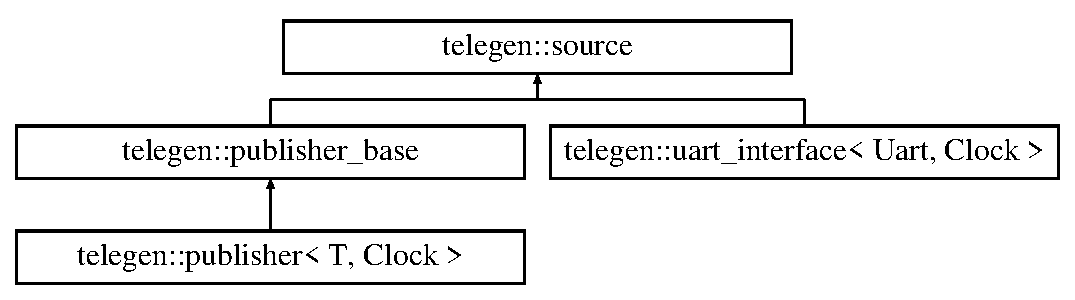
\includegraphics[height=3.000000cm]{classtelegen_1_1source}
\end{center}
\end{figure}
\subsection*{Public Member Functions}
\begin{DoxyCompactItemize}
\item 
virtual \hyperlink{namespacetelegen_a9dd802bb5d30cf96b0c616750d43ae86}{promise}$<$ \hyperlink{namespacetelegen_a27c822534a5231fe1c523c81e8768afb}{subscription\+\_\+ptr} $>$ \hyperlink{classtelegen_1_1source_a224b4eb02ea346aca099615a5ae00ea9}{subscribe} (\hyperlink{classtelegen_1_1variable__base}{variable\+\_\+base} $\ast$v, \hyperlink{namespacetelegen_ad925de2d0a99bc43918533abf0457344}{interval} min\+\_\+interval, \hyperlink{namespacetelegen_ad925de2d0a99bc43918533abf0457344}{interval} max\+\_\+interval, \hyperlink{namespacetelegen_ad925de2d0a99bc43918533abf0457344}{interval} timeout)=0
\item 
virtual \hyperlink{namespacetelegen_a9dd802bb5d30cf96b0c616750d43ae86}{promise}$<$ \hyperlink{classtelegen_1_1value}{value} $>$ \hyperlink{classtelegen_1_1source_ae14191b0e6aa10521bb3d8fa5e1747e9}{call} (\hyperlink{classtelegen_1_1action__base}{action\+\_\+base} $\ast$a, \hyperlink{classtelegen_1_1value}{value} arg, \hyperlink{namespacetelegen_ad925de2d0a99bc43918533abf0457344}{interval} timeout)=0
\end{DoxyCompactItemize}


\subsection{Member Function Documentation}
\mbox{\Hypertarget{classtelegen_1_1source_ae14191b0e6aa10521bb3d8fa5e1747e9}\label{classtelegen_1_1source_ae14191b0e6aa10521bb3d8fa5e1747e9}} 
\index{telegen\+::source@{telegen\+::source}!call@{call}}
\index{call@{call}!telegen\+::source@{telegen\+::source}}
\subsubsection{\texorpdfstring{call()}{call()}}
{\footnotesize\ttfamily virtual \hyperlink{namespacetelegen_a9dd802bb5d30cf96b0c616750d43ae86}{promise}$<$\hyperlink{classtelegen_1_1value}{value}$>$ telegen\+::source\+::call (\begin{DoxyParamCaption}\item[{\hyperlink{classtelegen_1_1action__base}{action\+\_\+base} $\ast$}]{a,  }\item[{\hyperlink{classtelegen_1_1value}{value}}]{arg,  }\item[{\hyperlink{namespacetelegen_ad925de2d0a99bc43918533abf0457344}{interval}}]{timeout }\end{DoxyParamCaption})\hspace{0.3cm}{\ttfamily [pure virtual]}}



Implemented in \hyperlink{classtelegen_1_1publisher_a3b5f514d064a6bca0209753dd724a2a7}{telegen\+::publisher$<$ T, Clock $>$}, and \hyperlink{classtelegen_1_1uart__interface_acaf4ff8f9442b3d4d2b9d5bcc252d08e}{telegen\+::uart\+\_\+interface$<$ Uart, Clock $>$}.

\mbox{\Hypertarget{classtelegen_1_1source_a224b4eb02ea346aca099615a5ae00ea9}\label{classtelegen_1_1source_a224b4eb02ea346aca099615a5ae00ea9}} 
\index{telegen\+::source@{telegen\+::source}!subscribe@{subscribe}}
\index{subscribe@{subscribe}!telegen\+::source@{telegen\+::source}}
\subsubsection{\texorpdfstring{subscribe()}{subscribe()}}
{\footnotesize\ttfamily virtual \hyperlink{namespacetelegen_a9dd802bb5d30cf96b0c616750d43ae86}{promise}$<$\hyperlink{namespacetelegen_a27c822534a5231fe1c523c81e8768afb}{subscription\+\_\+ptr}$>$ telegen\+::source\+::subscribe (\begin{DoxyParamCaption}\item[{\hyperlink{classtelegen_1_1variable__base}{variable\+\_\+base} $\ast$}]{v,  }\item[{\hyperlink{namespacetelegen_ad925de2d0a99bc43918533abf0457344}{interval}}]{min\+\_\+interval,  }\item[{\hyperlink{namespacetelegen_ad925de2d0a99bc43918533abf0457344}{interval}}]{max\+\_\+interval,  }\item[{\hyperlink{namespacetelegen_ad925de2d0a99bc43918533abf0457344}{interval}}]{timeout }\end{DoxyParamCaption})\hspace{0.3cm}{\ttfamily [pure virtual]}}



Implemented in \hyperlink{classtelegen_1_1publisher_abb9ec30f9b0859e34111dc02fe8b52bd}{telegen\+::publisher$<$ T, Clock $>$}, and \hyperlink{classtelegen_1_1uart__interface_a869d06375865913880cf9818150c5b6e}{telegen\+::uart\+\_\+interface$<$ Uart, Clock $>$}.



The documentation for this class was generated from the following file\+:\begin{DoxyCompactItemize}
\item 
\hyperlink{source_8hpp}{source.\+hpp}\end{DoxyCompactItemize}

\hypertarget{classtelegen_1_1sub}{}\section{telegen\+:\+:sub$<$ T $>$ Class Template Reference}
\label{classtelegen_1_1sub}\index{telegen\+::sub$<$ T $>$@{telegen\+::sub$<$ T $>$}}


{\ttfamily \#include $<$nodes.\+hpp$>$}

\subsection*{Public Member Functions}
\begin{DoxyCompactItemize}
\item 
\hyperlink{classtelegen_1_1sub_a90e40c9ecf240073689c04807f3cb43d}{sub} (std\+::unique\+\_\+ptr$<$ \hyperlink{classtelegen_1_1subscription}{subscription} $>$ \&\&s)
\item 
\hyperlink{classtelegen_1_1sub_aedfa8e90ccd9de1ec084e96ef42232cf}{sub} ()
\item 
void \hyperlink{classtelegen_1_1sub_ad1d7edeb15aea1ea4294919ae15faac2}{handler} (const std\+::function$<$ void(const T \&)$>$ \&cb)
\end{DoxyCompactItemize}


\subsection{Constructor \& Destructor Documentation}
\mbox{\Hypertarget{classtelegen_1_1sub_a90e40c9ecf240073689c04807f3cb43d}\label{classtelegen_1_1sub_a90e40c9ecf240073689c04807f3cb43d}} 
\index{telegen\+::sub@{telegen\+::sub}!sub@{sub}}
\index{sub@{sub}!telegen\+::sub@{telegen\+::sub}}
\subsubsection{\texorpdfstring{sub()}{sub()}\hspace{0.1cm}{\footnotesize\ttfamily [1/2]}}
{\footnotesize\ttfamily template$<$typename T $>$ \\
\hyperlink{classtelegen_1_1sub}{telegen\+::sub}$<$ T $>$\+::\hyperlink{classtelegen_1_1sub}{sub} (\begin{DoxyParamCaption}\item[{std\+::unique\+\_\+ptr$<$ \hyperlink{classtelegen_1_1subscription}{subscription} $>$ \&\&}]{s }\end{DoxyParamCaption})\hspace{0.3cm}{\ttfamily [inline]}}

\mbox{\Hypertarget{classtelegen_1_1sub_aedfa8e90ccd9de1ec084e96ef42232cf}\label{classtelegen_1_1sub_aedfa8e90ccd9de1ec084e96ef42232cf}} 
\index{telegen\+::sub@{telegen\+::sub}!sub@{sub}}
\index{sub@{sub}!telegen\+::sub@{telegen\+::sub}}
\subsubsection{\texorpdfstring{sub()}{sub()}\hspace{0.1cm}{\footnotesize\ttfamily [2/2]}}
{\footnotesize\ttfamily template$<$typename T $>$ \\
\hyperlink{classtelegen_1_1sub}{telegen\+::sub}$<$ T $>$\+::\hyperlink{classtelegen_1_1sub}{sub} (\begin{DoxyParamCaption}{ }\end{DoxyParamCaption})\hspace{0.3cm}{\ttfamily [inline]}}



\subsection{Member Function Documentation}
\mbox{\Hypertarget{classtelegen_1_1sub_ad1d7edeb15aea1ea4294919ae15faac2}\label{classtelegen_1_1sub_ad1d7edeb15aea1ea4294919ae15faac2}} 
\index{telegen\+::sub@{telegen\+::sub}!handler@{handler}}
\index{handler@{handler}!telegen\+::sub@{telegen\+::sub}}
\subsubsection{\texorpdfstring{handler()}{handler()}}
{\footnotesize\ttfamily template$<$typename T $>$ \\
void \hyperlink{classtelegen_1_1sub}{telegen\+::sub}$<$ T $>$\+::handler (\begin{DoxyParamCaption}\item[{const std\+::function$<$ void(const T \&)$>$ \&}]{cb }\end{DoxyParamCaption})\hspace{0.3cm}{\ttfamily [inline]}}



The documentation for this class was generated from the following file\+:\begin{DoxyCompactItemize}
\item 
\hyperlink{gen_2telegen_2nodes_8hpp}{gen/telegen/nodes.\+hpp}\end{DoxyCompactItemize}

\hypertarget{classtelegen_1_1publisher_1_1sub__impl}{}\section{telegen\+:\+:publisher$<$ T, Clock $>$\+:\+:sub\+\_\+impl Class Reference}
\label{classtelegen_1_1publisher_1_1sub__impl}\index{telegen\+::publisher$<$ T, Clock $>$\+::sub\+\_\+impl@{telegen\+::publisher$<$ T, Clock $>$\+::sub\+\_\+impl}}


{\ttfamily \#include $<$publisher.\+hpp$>$}

Inheritance diagram for telegen\+:\+:publisher$<$ T, Clock $>$\+:\+:sub\+\_\+impl\+:\begin{figure}[H]
\begin{center}
\leavevmode
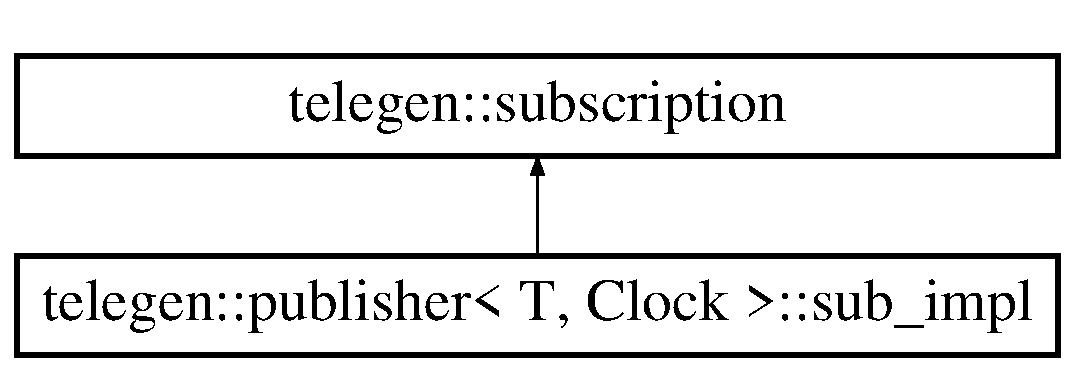
\includegraphics[height=2.000000cm]{classtelegen_1_1publisher_1_1sub__impl}
\end{center}
\end{figure}
\subsection*{Public Member Functions}
\begin{DoxyCompactItemize}
\item 
\hyperlink{classtelegen_1_1publisher_1_1sub__impl_af79e7e1cbc3f4eb803b42438328a1bb1}{sub\+\_\+impl} (\hyperlink{classtelegen_1_1publisher}{publisher}$<$ T, Clock $>$ $\ast$pub, int32\+\_\+t min\+\_\+interval, int32\+\_\+t max\+\_\+interval)
\item 
\hyperlink{classtelegen_1_1publisher_1_1sub__impl_a91197bedcf945e62ca5ab0a5cd577081}{$\sim$sub\+\_\+impl} ()
\item 
bool \hyperlink{classtelegen_1_1publisher_1_1sub__impl_a9880e80ac0b1887b5aec423abbc0a6f3}{is\+\_\+cancelled} () override
\item 
\hyperlink{namespacetelegen_a9dd802bb5d30cf96b0c616750d43ae86}{promise} \hyperlink{classtelegen_1_1publisher_1_1sub__impl_ae0a84e8e0a45d21c688ee557c603c43d}{cancel} (\hyperlink{namespacetelegen_ad925de2d0a99bc43918533abf0457344}{interval} timeout) override
\item 
\hyperlink{namespacetelegen_a9dd802bb5d30cf96b0c616750d43ae86}{promise} \hyperlink{classtelegen_1_1publisher_1_1sub__impl_a2144a27beee3ef15a21fb7fd323b3770}{change} (\hyperlink{namespacetelegen_ad925de2d0a99bc43918533abf0457344}{interval} min\+\_\+int, \hyperlink{namespacetelegen_ad925de2d0a99bc43918533abf0457344}{interval} max\+\_\+int, \hyperlink{namespacetelegen_ad925de2d0a99bc43918533abf0457344}{interval} timeout) override
\item 
void \hyperlink{classtelegen_1_1publisher_1_1sub__impl_a9d4f5e7d31c57067abccddeca51adbb0}{push} (const T \&v, int32\+\_\+t now\+\_\+time)
\item 
void \hyperlink{classtelegen_1_1publisher_1_1sub__impl_a282c0e002c00b8649ca7b450fc35fd4f}{push\+\_\+delayed} (const T \&v, uint32\+\_\+t now\+\_\+time)
\item 
void \hyperlink{classtelegen_1_1publisher_1_1sub__impl_a3e36c9dec7f667891bb879ceae529879}{push\+\_\+resend} (const T \&v, int32\+\_\+t now\+\_\+time)
\end{DoxyCompactItemize}
\subsection*{Public Attributes}
\begin{DoxyCompactItemize}
\item 
uint32\+\_\+t \hyperlink{classtelegen_1_1publisher_1_1sub__impl_a479b96db21c40241b6eefca3e8c66f25}{last\+\_\+time\+\_\+}
\item 
uint32\+\_\+t \hyperlink{classtelegen_1_1publisher_1_1sub__impl_af732353e21826cd15007a6d7a5e315a5}{delay\+\_\+alarm\+\_\+}
\item 
uint32\+\_\+t \hyperlink{classtelegen_1_1publisher_1_1sub__impl_a087771e828beef87096487ac4e2e41ad}{resend\+\_\+alarm\+\_\+}
\item 
\hyperlink{classtelegen_1_1publisher}{publisher}$<$ T, Clock $>$ $\ast$ \hyperlink{classtelegen_1_1publisher_1_1sub__impl_a3433861f175df3cce9e1af5f03b0a076}{pub\+\_\+}
\end{DoxyCompactItemize}
\subsection*{Additional Inherited Members}


\subsection{Constructor \& Destructor Documentation}
\mbox{\Hypertarget{classtelegen_1_1publisher_1_1sub__impl_af79e7e1cbc3f4eb803b42438328a1bb1}\label{classtelegen_1_1publisher_1_1sub__impl_af79e7e1cbc3f4eb803b42438328a1bb1}} 
\index{telegen\+::publisher\+::sub\+\_\+impl@{telegen\+::publisher\+::sub\+\_\+impl}!sub\+\_\+impl@{sub\+\_\+impl}}
\index{sub\+\_\+impl@{sub\+\_\+impl}!telegen\+::publisher\+::sub\+\_\+impl@{telegen\+::publisher\+::sub\+\_\+impl}}
\subsubsection{\texorpdfstring{sub\+\_\+impl()}{sub\_impl()}}
{\footnotesize\ttfamily template$<$typename T, typename Clock$>$ \\
\hyperlink{classtelegen_1_1publisher}{telegen\+::publisher}$<$ T, Clock $>$\+::sub\+\_\+impl\+::sub\+\_\+impl (\begin{DoxyParamCaption}\item[{\hyperlink{classtelegen_1_1publisher}{publisher}$<$ T, Clock $>$ $\ast$}]{pub,  }\item[{int32\+\_\+t}]{min\+\_\+interval,  }\item[{int32\+\_\+t}]{max\+\_\+interval }\end{DoxyParamCaption})\hspace{0.3cm}{\ttfamily [inline]}}

\mbox{\Hypertarget{classtelegen_1_1publisher_1_1sub__impl_a91197bedcf945e62ca5ab0a5cd577081}\label{classtelegen_1_1publisher_1_1sub__impl_a91197bedcf945e62ca5ab0a5cd577081}} 
\index{telegen\+::publisher\+::sub\+\_\+impl@{telegen\+::publisher\+::sub\+\_\+impl}!````~sub\+\_\+impl@{$\sim$sub\+\_\+impl}}
\index{````~sub\+\_\+impl@{$\sim$sub\+\_\+impl}!telegen\+::publisher\+::sub\+\_\+impl@{telegen\+::publisher\+::sub\+\_\+impl}}
\subsubsection{\texorpdfstring{$\sim$sub\+\_\+impl()}{~sub\_impl()}}
{\footnotesize\ttfamily template$<$typename T, typename Clock$>$ \\
\hyperlink{classtelegen_1_1publisher}{telegen\+::publisher}$<$ T, Clock $>$\+::sub\+\_\+impl\+::$\sim$sub\+\_\+impl (\begin{DoxyParamCaption}{ }\end{DoxyParamCaption})\hspace{0.3cm}{\ttfamily [inline]}}



\subsection{Member Function Documentation}
\mbox{\Hypertarget{classtelegen_1_1publisher_1_1sub__impl_ae0a84e8e0a45d21c688ee557c603c43d}\label{classtelegen_1_1publisher_1_1sub__impl_ae0a84e8e0a45d21c688ee557c603c43d}} 
\index{telegen\+::publisher\+::sub\+\_\+impl@{telegen\+::publisher\+::sub\+\_\+impl}!cancel@{cancel}}
\index{cancel@{cancel}!telegen\+::publisher\+::sub\+\_\+impl@{telegen\+::publisher\+::sub\+\_\+impl}}
\subsubsection{\texorpdfstring{cancel()}{cancel()}}
{\footnotesize\ttfamily template$<$typename T, typename Clock$>$ \\
\hyperlink{namespacetelegen_a9dd802bb5d30cf96b0c616750d43ae86}{promise} \hyperlink{classtelegen_1_1publisher}{telegen\+::publisher}$<$ T, Clock $>$\+::sub\+\_\+impl\+::cancel (\begin{DoxyParamCaption}\item[{\hyperlink{namespacetelegen_ad925de2d0a99bc43918533abf0457344}{interval}}]{timeout }\end{DoxyParamCaption})\hspace{0.3cm}{\ttfamily [inline]}, {\ttfamily [override]}, {\ttfamily [virtual]}}



Implements \hyperlink{classtelegen_1_1subscription_a7d645e1bf76477316d9f868a69467e42}{telegen\+::subscription}.

\mbox{\Hypertarget{classtelegen_1_1publisher_1_1sub__impl_a2144a27beee3ef15a21fb7fd323b3770}\label{classtelegen_1_1publisher_1_1sub__impl_a2144a27beee3ef15a21fb7fd323b3770}} 
\index{telegen\+::publisher\+::sub\+\_\+impl@{telegen\+::publisher\+::sub\+\_\+impl}!change@{change}}
\index{change@{change}!telegen\+::publisher\+::sub\+\_\+impl@{telegen\+::publisher\+::sub\+\_\+impl}}
\subsubsection{\texorpdfstring{change()}{change()}}
{\footnotesize\ttfamily template$<$typename T, typename Clock$>$ \\
\hyperlink{namespacetelegen_a9dd802bb5d30cf96b0c616750d43ae86}{promise} \hyperlink{classtelegen_1_1publisher}{telegen\+::publisher}$<$ T, Clock $>$\+::sub\+\_\+impl\+::change (\begin{DoxyParamCaption}\item[{\hyperlink{namespacetelegen_ad925de2d0a99bc43918533abf0457344}{interval}}]{min\+\_\+int,  }\item[{\hyperlink{namespacetelegen_ad925de2d0a99bc43918533abf0457344}{interval}}]{max\+\_\+int,  }\item[{\hyperlink{namespacetelegen_ad925de2d0a99bc43918533abf0457344}{interval}}]{timeout }\end{DoxyParamCaption})\hspace{0.3cm}{\ttfamily [inline]}, {\ttfamily [override]}, {\ttfamily [virtual]}}



Implements \hyperlink{classtelegen_1_1subscription_aca992d1891107380ec81a517ea0bde58}{telegen\+::subscription}.

\mbox{\Hypertarget{classtelegen_1_1publisher_1_1sub__impl_a9880e80ac0b1887b5aec423abbc0a6f3}\label{classtelegen_1_1publisher_1_1sub__impl_a9880e80ac0b1887b5aec423abbc0a6f3}} 
\index{telegen\+::publisher\+::sub\+\_\+impl@{telegen\+::publisher\+::sub\+\_\+impl}!is\+\_\+cancelled@{is\+\_\+cancelled}}
\index{is\+\_\+cancelled@{is\+\_\+cancelled}!telegen\+::publisher\+::sub\+\_\+impl@{telegen\+::publisher\+::sub\+\_\+impl}}
\subsubsection{\texorpdfstring{is\+\_\+cancelled()}{is\_cancelled()}}
{\footnotesize\ttfamily template$<$typename T, typename Clock$>$ \\
bool \hyperlink{classtelegen_1_1publisher}{telegen\+::publisher}$<$ T, Clock $>$\+::sub\+\_\+impl\+::is\+\_\+cancelled (\begin{DoxyParamCaption}{ }\end{DoxyParamCaption})\hspace{0.3cm}{\ttfamily [inline]}, {\ttfamily [override]}, {\ttfamily [virtual]}}



Implements \hyperlink{classtelegen_1_1subscription_a4bbe4edbb2ecba3ccff4d6de562e2e7d}{telegen\+::subscription}.

\mbox{\Hypertarget{classtelegen_1_1publisher_1_1sub__impl_a9d4f5e7d31c57067abccddeca51adbb0}\label{classtelegen_1_1publisher_1_1sub__impl_a9d4f5e7d31c57067abccddeca51adbb0}} 
\index{telegen\+::publisher\+::sub\+\_\+impl@{telegen\+::publisher\+::sub\+\_\+impl}!push@{push}}
\index{push@{push}!telegen\+::publisher\+::sub\+\_\+impl@{telegen\+::publisher\+::sub\+\_\+impl}}
\subsubsection{\texorpdfstring{push()}{push()}}
{\footnotesize\ttfamily template$<$typename T, typename Clock$>$ \\
void \hyperlink{classtelegen_1_1publisher}{telegen\+::publisher}$<$ T, Clock $>$\+::sub\+\_\+impl\+::push (\begin{DoxyParamCaption}\item[{const T \&}]{v,  }\item[{int32\+\_\+t}]{now\+\_\+time }\end{DoxyParamCaption})\hspace{0.3cm}{\ttfamily [inline]}}

\mbox{\Hypertarget{classtelegen_1_1publisher_1_1sub__impl_a282c0e002c00b8649ca7b450fc35fd4f}\label{classtelegen_1_1publisher_1_1sub__impl_a282c0e002c00b8649ca7b450fc35fd4f}} 
\index{telegen\+::publisher\+::sub\+\_\+impl@{telegen\+::publisher\+::sub\+\_\+impl}!push\+\_\+delayed@{push\+\_\+delayed}}
\index{push\+\_\+delayed@{push\+\_\+delayed}!telegen\+::publisher\+::sub\+\_\+impl@{telegen\+::publisher\+::sub\+\_\+impl}}
\subsubsection{\texorpdfstring{push\+\_\+delayed()}{push\_delayed()}}
{\footnotesize\ttfamily template$<$typename T, typename Clock$>$ \\
void \hyperlink{classtelegen_1_1publisher}{telegen\+::publisher}$<$ T, Clock $>$\+::sub\+\_\+impl\+::push\+\_\+delayed (\begin{DoxyParamCaption}\item[{const T \&}]{v,  }\item[{uint32\+\_\+t}]{now\+\_\+time }\end{DoxyParamCaption})\hspace{0.3cm}{\ttfamily [inline]}}

\mbox{\Hypertarget{classtelegen_1_1publisher_1_1sub__impl_a3e36c9dec7f667891bb879ceae529879}\label{classtelegen_1_1publisher_1_1sub__impl_a3e36c9dec7f667891bb879ceae529879}} 
\index{telegen\+::publisher\+::sub\+\_\+impl@{telegen\+::publisher\+::sub\+\_\+impl}!push\+\_\+resend@{push\+\_\+resend}}
\index{push\+\_\+resend@{push\+\_\+resend}!telegen\+::publisher\+::sub\+\_\+impl@{telegen\+::publisher\+::sub\+\_\+impl}}
\subsubsection{\texorpdfstring{push\+\_\+resend()}{push\_resend()}}
{\footnotesize\ttfamily template$<$typename T, typename Clock$>$ \\
void \hyperlink{classtelegen_1_1publisher}{telegen\+::publisher}$<$ T, Clock $>$\+::sub\+\_\+impl\+::push\+\_\+resend (\begin{DoxyParamCaption}\item[{const T \&}]{v,  }\item[{int32\+\_\+t}]{now\+\_\+time }\end{DoxyParamCaption})\hspace{0.3cm}{\ttfamily [inline]}}



\subsection{Member Data Documentation}
\mbox{\Hypertarget{classtelegen_1_1publisher_1_1sub__impl_af732353e21826cd15007a6d7a5e315a5}\label{classtelegen_1_1publisher_1_1sub__impl_af732353e21826cd15007a6d7a5e315a5}} 
\index{telegen\+::publisher\+::sub\+\_\+impl@{telegen\+::publisher\+::sub\+\_\+impl}!delay\+\_\+alarm\+\_\+@{delay\+\_\+alarm\+\_\+}}
\index{delay\+\_\+alarm\+\_\+@{delay\+\_\+alarm\+\_\+}!telegen\+::publisher\+::sub\+\_\+impl@{telegen\+::publisher\+::sub\+\_\+impl}}
\subsubsection{\texorpdfstring{delay\+\_\+alarm\+\_\+}{delay\_alarm\_}}
{\footnotesize\ttfamily template$<$typename T, typename Clock$>$ \\
uint32\+\_\+t \hyperlink{classtelegen_1_1publisher}{telegen\+::publisher}$<$ T, Clock $>$\+::sub\+\_\+impl\+::delay\+\_\+alarm\+\_\+}

\mbox{\Hypertarget{classtelegen_1_1publisher_1_1sub__impl_a479b96db21c40241b6eefca3e8c66f25}\label{classtelegen_1_1publisher_1_1sub__impl_a479b96db21c40241b6eefca3e8c66f25}} 
\index{telegen\+::publisher\+::sub\+\_\+impl@{telegen\+::publisher\+::sub\+\_\+impl}!last\+\_\+time\+\_\+@{last\+\_\+time\+\_\+}}
\index{last\+\_\+time\+\_\+@{last\+\_\+time\+\_\+}!telegen\+::publisher\+::sub\+\_\+impl@{telegen\+::publisher\+::sub\+\_\+impl}}
\subsubsection{\texorpdfstring{last\+\_\+time\+\_\+}{last\_time\_}}
{\footnotesize\ttfamily template$<$typename T, typename Clock$>$ \\
uint32\+\_\+t \hyperlink{classtelegen_1_1publisher}{telegen\+::publisher}$<$ T, Clock $>$\+::sub\+\_\+impl\+::last\+\_\+time\+\_\+}

\mbox{\Hypertarget{classtelegen_1_1publisher_1_1sub__impl_a3433861f175df3cce9e1af5f03b0a076}\label{classtelegen_1_1publisher_1_1sub__impl_a3433861f175df3cce9e1af5f03b0a076}} 
\index{telegen\+::publisher\+::sub\+\_\+impl@{telegen\+::publisher\+::sub\+\_\+impl}!pub\+\_\+@{pub\+\_\+}}
\index{pub\+\_\+@{pub\+\_\+}!telegen\+::publisher\+::sub\+\_\+impl@{telegen\+::publisher\+::sub\+\_\+impl}}
\subsubsection{\texorpdfstring{pub\+\_\+}{pub\_}}
{\footnotesize\ttfamily template$<$typename T, typename Clock$>$ \\
\hyperlink{classtelegen_1_1publisher}{publisher}$<$T, Clock$>$$\ast$ \hyperlink{classtelegen_1_1publisher}{telegen\+::publisher}$<$ T, Clock $>$\+::sub\+\_\+impl\+::pub\+\_\+}

\mbox{\Hypertarget{classtelegen_1_1publisher_1_1sub__impl_a087771e828beef87096487ac4e2e41ad}\label{classtelegen_1_1publisher_1_1sub__impl_a087771e828beef87096487ac4e2e41ad}} 
\index{telegen\+::publisher\+::sub\+\_\+impl@{telegen\+::publisher\+::sub\+\_\+impl}!resend\+\_\+alarm\+\_\+@{resend\+\_\+alarm\+\_\+}}
\index{resend\+\_\+alarm\+\_\+@{resend\+\_\+alarm\+\_\+}!telegen\+::publisher\+::sub\+\_\+impl@{telegen\+::publisher\+::sub\+\_\+impl}}
\subsubsection{\texorpdfstring{resend\+\_\+alarm\+\_\+}{resend\_alarm\_}}
{\footnotesize\ttfamily template$<$typename T, typename Clock$>$ \\
uint32\+\_\+t \hyperlink{classtelegen_1_1publisher}{telegen\+::publisher}$<$ T, Clock $>$\+::sub\+\_\+impl\+::resend\+\_\+alarm\+\_\+}



The documentation for this class was generated from the following file\+:\begin{DoxyCompactItemize}
\item 
\hyperlink{gen_2telegen_2publisher_8hpp}{gen/telegen/publisher.\+hpp}\end{DoxyCompactItemize}

\hypertarget{classtelegraph_1_1subscription}{}\section{telegraph\+:\+:subscription Class Reference}
\label{classtelegraph_1_1subscription}\index{telegraph\+::subscription@{telegraph\+::subscription}}


{\ttfamily \#include $<$data.\+hpp$>$}

\subsection*{Public Member Functions}
\begin{DoxyCompactItemize}
\item 
\hyperlink{classtelegraph_1_1subscription_ae4c98364487057db2aa99675dac8afb5}{subscription} (\hyperlink{classtelegraph_1_1value__type}{value\+\_\+type} t, float debounce, float refresh)
\item 
virtual \hyperlink{classtelegraph_1_1subscription_a8a9cf662e9a068514d9595d9df0a48ca}{$\sim$subscription} ()
\item 
constexpr const \hyperlink{classtelegraph_1_1value__type}{value\+\_\+type} \& \hyperlink{classtelegraph_1_1subscription_a9a574364550840ba96c594a4dab83b9e}{get\+\_\+type} () const
\item 
constexpr float \hyperlink{classtelegraph_1_1subscription_a8ce2ae85cf733760222ed81db2791acf}{get\+\_\+debounce} () const
\item 
constexpr float \hyperlink{classtelegraph_1_1subscription_a92eb73e4f104fefbdfe886ec8122a2b7}{get\+\_\+refresh} () const
\item 
constexpr bool \hyperlink{classtelegraph_1_1subscription_a9dc4805fc25661d3901e8a4181e2e0f1}{is\+\_\+cancelled} () const
\item 
virtual void \hyperlink{classtelegraph_1_1subscription_a55d47626d788e73317c5b8525d1369ff}{poll} ()=0
\item 
virtual void \hyperlink{classtelegraph_1_1subscription_a18cf566e14d908c2403bb31a4114f3b9}{change} (\hyperlink{structboost_1_1asio_1_1yield__ctx}{io\+::yield\+\_\+ctx} \&, float debounce, float refresh, float timeout)=0
\item 
virtual void \hyperlink{classtelegraph_1_1subscription_ae8efc1bddc19862bf79ea2659e3ae980}{cancel} (\hyperlink{structboost_1_1asio_1_1yield__ctx}{io\+::yield\+\_\+ctx} \&yield, float timeout)=0
\item 
virtual void \hyperlink{classtelegraph_1_1subscription_aa4917994240c530af2fd0e2a5bff435c}{cancel} ()=0
\end{DoxyCompactItemize}
\subsection*{Public Attributes}
\begin{DoxyCompactItemize}
\item 
\hyperlink{classtelegraph_1_1signal}{signal}$<$ \hyperlink{classtelegraph_1_1value}{value} $>$ \hyperlink{classtelegraph_1_1subscription_adaaff860567d8a1dd105cd1fcc91a840}{data}
\item 
\hyperlink{classtelegraph_1_1signal}{signal} \hyperlink{classtelegraph_1_1subscription_af871f21ea83b527626725c9fedc247f2}{cancelled}
\end{DoxyCompactItemize}
\subsection*{Static Public Attributes}
\begin{DoxyCompactItemize}
\item 
static constexpr float \hyperlink{classtelegraph_1_1subscription_a193bc79b41f19075b015c7af7c1f7738}{D\+I\+S\+A\+B\+L\+ED} = std\+::numeric\+\_\+limits$<$float$>$\+::infinity()
\end{DoxyCompactItemize}
\subsection*{Protected Attributes}
\begin{DoxyCompactItemize}
\item 
bool \hyperlink{classtelegraph_1_1subscription_a4a52c45f257a495f0ced91d5e9cc3723}{cancelled\+\_\+}
\item 
\hyperlink{classtelegraph_1_1value__type}{value\+\_\+type} \hyperlink{classtelegraph_1_1subscription_a1f168a6bb8f030ebc870e1a702192139}{type\+\_\+}
\item 
float \hyperlink{classtelegraph_1_1subscription_a81abb8423637f2519d24a319f3f45cf0}{debounce\+\_\+}
\item 
float \hyperlink{classtelegraph_1_1subscription_aaae42162bcfb0f4e6e75f4a3e36de6d9}{refresh\+\_\+}
\end{DoxyCompactItemize}


\subsection{Constructor \& Destructor Documentation}
\mbox{\Hypertarget{classtelegraph_1_1subscription_ae4c98364487057db2aa99675dac8afb5}\label{classtelegraph_1_1subscription_ae4c98364487057db2aa99675dac8afb5}} 
\index{telegraph\+::subscription@{telegraph\+::subscription}!subscription@{subscription}}
\index{subscription@{subscription}!telegraph\+::subscription@{telegraph\+::subscription}}
\subsubsection{\texorpdfstring{subscription()}{subscription()}}
{\footnotesize\ttfamily telegraph\+::subscription\+::subscription (\begin{DoxyParamCaption}\item[{\hyperlink{classtelegraph_1_1value__type}{value\+\_\+type}}]{t,  }\item[{float}]{debounce,  }\item[{float}]{refresh }\end{DoxyParamCaption})\hspace{0.3cm}{\ttfamily [inline]}}

\mbox{\Hypertarget{classtelegraph_1_1subscription_a8a9cf662e9a068514d9595d9df0a48ca}\label{classtelegraph_1_1subscription_a8a9cf662e9a068514d9595d9df0a48ca}} 
\index{telegraph\+::subscription@{telegraph\+::subscription}!````~subscription@{$\sim$subscription}}
\index{````~subscription@{$\sim$subscription}!telegraph\+::subscription@{telegraph\+::subscription}}
\subsubsection{\texorpdfstring{$\sim$subscription()}{~subscription()}}
{\footnotesize\ttfamily virtual telegraph\+::subscription\+::$\sim$subscription (\begin{DoxyParamCaption}{ }\end{DoxyParamCaption})\hspace{0.3cm}{\ttfamily [inline]}, {\ttfamily [virtual]}}

On destruction \hyperlink{classtelegraph_1_1subscription_aa4917994240c530af2fd0e2a5bff435c}{cancel()} should be triggered 

\subsection{Member Function Documentation}
\mbox{\Hypertarget{classtelegraph_1_1subscription_ae8efc1bddc19862bf79ea2659e3ae980}\label{classtelegraph_1_1subscription_ae8efc1bddc19862bf79ea2659e3ae980}} 
\index{telegraph\+::subscription@{telegraph\+::subscription}!cancel@{cancel}}
\index{cancel@{cancel}!telegraph\+::subscription@{telegraph\+::subscription}}
\subsubsection{\texorpdfstring{cancel()}{cancel()}\hspace{0.1cm}{\footnotesize\ttfamily [1/2]}}
{\footnotesize\ttfamily virtual void telegraph\+::subscription\+::cancel (\begin{DoxyParamCaption}\item[{\hyperlink{structboost_1_1asio_1_1yield__ctx}{io\+::yield\+\_\+ctx} \&}]{yield,  }\item[{float}]{timeout }\end{DoxyParamCaption})\hspace{0.3cm}{\ttfamily [pure virtual]}}

\mbox{\Hypertarget{classtelegraph_1_1subscription_aa4917994240c530af2fd0e2a5bff435c}\label{classtelegraph_1_1subscription_aa4917994240c530af2fd0e2a5bff435c}} 
\index{telegraph\+::subscription@{telegraph\+::subscription}!cancel@{cancel}}
\index{cancel@{cancel}!telegraph\+::subscription@{telegraph\+::subscription}}
\subsubsection{\texorpdfstring{cancel()}{cancel()}\hspace{0.1cm}{\footnotesize\ttfamily [2/2]}}
{\footnotesize\ttfamily virtual void telegraph\+::subscription\+::cancel (\begin{DoxyParamCaption}{ }\end{DoxyParamCaption})\hspace{0.3cm}{\ttfamily [pure virtual]}}

\mbox{\Hypertarget{classtelegraph_1_1subscription_a18cf566e14d908c2403bb31a4114f3b9}\label{classtelegraph_1_1subscription_a18cf566e14d908c2403bb31a4114f3b9}} 
\index{telegraph\+::subscription@{telegraph\+::subscription}!change@{change}}
\index{change@{change}!telegraph\+::subscription@{telegraph\+::subscription}}
\subsubsection{\texorpdfstring{change()}{change()}}
{\footnotesize\ttfamily virtual void telegraph\+::subscription\+::change (\begin{DoxyParamCaption}\item[{\hyperlink{structboost_1_1asio_1_1yield__ctx}{io\+::yield\+\_\+ctx} \&}]{,  }\item[{float}]{debounce,  }\item[{float}]{refresh,  }\item[{float}]{timeout }\end{DoxyParamCaption})\hspace{0.3cm}{\ttfamily [pure virtual]}}

\mbox{\Hypertarget{classtelegraph_1_1subscription_a8ce2ae85cf733760222ed81db2791acf}\label{classtelegraph_1_1subscription_a8ce2ae85cf733760222ed81db2791acf}} 
\index{telegraph\+::subscription@{telegraph\+::subscription}!get\+\_\+debounce@{get\+\_\+debounce}}
\index{get\+\_\+debounce@{get\+\_\+debounce}!telegraph\+::subscription@{telegraph\+::subscription}}
\subsubsection{\texorpdfstring{get\+\_\+debounce()}{get\_debounce()}}
{\footnotesize\ttfamily constexpr float telegraph\+::subscription\+::get\+\_\+debounce (\begin{DoxyParamCaption}{ }\end{DoxyParamCaption}) const\hspace{0.3cm}{\ttfamily [inline]}}

\mbox{\Hypertarget{classtelegraph_1_1subscription_a92eb73e4f104fefbdfe886ec8122a2b7}\label{classtelegraph_1_1subscription_a92eb73e4f104fefbdfe886ec8122a2b7}} 
\index{telegraph\+::subscription@{telegraph\+::subscription}!get\+\_\+refresh@{get\+\_\+refresh}}
\index{get\+\_\+refresh@{get\+\_\+refresh}!telegraph\+::subscription@{telegraph\+::subscription}}
\subsubsection{\texorpdfstring{get\+\_\+refresh()}{get\_refresh()}}
{\footnotesize\ttfamily constexpr float telegraph\+::subscription\+::get\+\_\+refresh (\begin{DoxyParamCaption}{ }\end{DoxyParamCaption}) const\hspace{0.3cm}{\ttfamily [inline]}}

\mbox{\Hypertarget{classtelegraph_1_1subscription_a9a574364550840ba96c594a4dab83b9e}\label{classtelegraph_1_1subscription_a9a574364550840ba96c594a4dab83b9e}} 
\index{telegraph\+::subscription@{telegraph\+::subscription}!get\+\_\+type@{get\+\_\+type}}
\index{get\+\_\+type@{get\+\_\+type}!telegraph\+::subscription@{telegraph\+::subscription}}
\subsubsection{\texorpdfstring{get\+\_\+type()}{get\_type()}}
{\footnotesize\ttfamily constexpr const \hyperlink{classtelegraph_1_1value__type}{value\+\_\+type}\& telegraph\+::subscription\+::get\+\_\+type (\begin{DoxyParamCaption}{ }\end{DoxyParamCaption}) const\hspace{0.3cm}{\ttfamily [inline]}}

\mbox{\Hypertarget{classtelegraph_1_1subscription_a9dc4805fc25661d3901e8a4181e2e0f1}\label{classtelegraph_1_1subscription_a9dc4805fc25661d3901e8a4181e2e0f1}} 
\index{telegraph\+::subscription@{telegraph\+::subscription}!is\+\_\+cancelled@{is\+\_\+cancelled}}
\index{is\+\_\+cancelled@{is\+\_\+cancelled}!telegraph\+::subscription@{telegraph\+::subscription}}
\subsubsection{\texorpdfstring{is\+\_\+cancelled()}{is\_cancelled()}}
{\footnotesize\ttfamily constexpr bool telegraph\+::subscription\+::is\+\_\+cancelled (\begin{DoxyParamCaption}{ }\end{DoxyParamCaption}) const\hspace{0.3cm}{\ttfamily [inline]}}

Whether this subscription is getting data \mbox{\Hypertarget{classtelegraph_1_1subscription_a55d47626d788e73317c5b8525d1369ff}\label{classtelegraph_1_1subscription_a55d47626d788e73317c5b8525d1369ff}} 
\index{telegraph\+::subscription@{telegraph\+::subscription}!poll@{poll}}
\index{poll@{poll}!telegraph\+::subscription@{telegraph\+::subscription}}
\subsubsection{\texorpdfstring{poll()}{poll()}}
{\footnotesize\ttfamily virtual void telegraph\+::subscription\+::poll (\begin{DoxyParamCaption}{ }\end{DoxyParamCaption})\hspace{0.3cm}{\ttfamily [pure virtual]}}



\subsection{Member Data Documentation}
\mbox{\Hypertarget{classtelegraph_1_1subscription_af871f21ea83b527626725c9fedc247f2}\label{classtelegraph_1_1subscription_af871f21ea83b527626725c9fedc247f2}} 
\index{telegraph\+::subscription@{telegraph\+::subscription}!cancelled@{cancelled}}
\index{cancelled@{cancelled}!telegraph\+::subscription@{telegraph\+::subscription}}
\subsubsection{\texorpdfstring{cancelled}{cancelled}}
{\footnotesize\ttfamily \hyperlink{classtelegraph_1_1signal}{signal} telegraph\+::subscription\+::cancelled}

\mbox{\Hypertarget{classtelegraph_1_1subscription_a4a52c45f257a495f0ced91d5e9cc3723}\label{classtelegraph_1_1subscription_a4a52c45f257a495f0ced91d5e9cc3723}} 
\index{telegraph\+::subscription@{telegraph\+::subscription}!cancelled\+\_\+@{cancelled\+\_\+}}
\index{cancelled\+\_\+@{cancelled\+\_\+}!telegraph\+::subscription@{telegraph\+::subscription}}
\subsubsection{\texorpdfstring{cancelled\+\_\+}{cancelled\_}}
{\footnotesize\ttfamily bool telegraph\+::subscription\+::cancelled\+\_\+\hspace{0.3cm}{\ttfamily [protected]}}

\mbox{\Hypertarget{classtelegraph_1_1subscription_adaaff860567d8a1dd105cd1fcc91a840}\label{classtelegraph_1_1subscription_adaaff860567d8a1dd105cd1fcc91a840}} 
\index{telegraph\+::subscription@{telegraph\+::subscription}!data@{data}}
\index{data@{data}!telegraph\+::subscription@{telegraph\+::subscription}}
\subsubsection{\texorpdfstring{data}{data}}
{\footnotesize\ttfamily \hyperlink{classtelegraph_1_1signal}{signal}$<$\hyperlink{classtelegraph_1_1value}{value}$>$ telegraph\+::subscription\+::data}

\mbox{\Hypertarget{classtelegraph_1_1subscription_a81abb8423637f2519d24a319f3f45cf0}\label{classtelegraph_1_1subscription_a81abb8423637f2519d24a319f3f45cf0}} 
\index{telegraph\+::subscription@{telegraph\+::subscription}!debounce\+\_\+@{debounce\+\_\+}}
\index{debounce\+\_\+@{debounce\+\_\+}!telegraph\+::subscription@{telegraph\+::subscription}}
\subsubsection{\texorpdfstring{debounce\+\_\+}{debounce\_}}
{\footnotesize\ttfamily float telegraph\+::subscription\+::debounce\+\_\+\hspace{0.3cm}{\ttfamily [protected]}}

\mbox{\Hypertarget{classtelegraph_1_1subscription_a193bc79b41f19075b015c7af7c1f7738}\label{classtelegraph_1_1subscription_a193bc79b41f19075b015c7af7c1f7738}} 
\index{telegraph\+::subscription@{telegraph\+::subscription}!D\+I\+S\+A\+B\+L\+ED@{D\+I\+S\+A\+B\+L\+ED}}
\index{D\+I\+S\+A\+B\+L\+ED@{D\+I\+S\+A\+B\+L\+ED}!telegraph\+::subscription@{telegraph\+::subscription}}
\subsubsection{\texorpdfstring{D\+I\+S\+A\+B\+L\+ED}{DISABLED}}
{\footnotesize\ttfamily constexpr float telegraph\+::subscription\+::\+D\+I\+S\+A\+B\+L\+ED = std\+::numeric\+\_\+limits$<$float$>$\+::infinity()\hspace{0.3cm}{\ttfamily [static]}}

\mbox{\Hypertarget{classtelegraph_1_1subscription_aaae42162bcfb0f4e6e75f4a3e36de6d9}\label{classtelegraph_1_1subscription_aaae42162bcfb0f4e6e75f4a3e36de6d9}} 
\index{telegraph\+::subscription@{telegraph\+::subscription}!refresh\+\_\+@{refresh\+\_\+}}
\index{refresh\+\_\+@{refresh\+\_\+}!telegraph\+::subscription@{telegraph\+::subscription}}
\subsubsection{\texorpdfstring{refresh\+\_\+}{refresh\_}}
{\footnotesize\ttfamily float telegraph\+::subscription\+::refresh\+\_\+\hspace{0.3cm}{\ttfamily [protected]}}

\mbox{\Hypertarget{classtelegraph_1_1subscription_a1f168a6bb8f030ebc870e1a702192139}\label{classtelegraph_1_1subscription_a1f168a6bb8f030ebc870e1a702192139}} 
\index{telegraph\+::subscription@{telegraph\+::subscription}!type\+\_\+@{type\+\_\+}}
\index{type\+\_\+@{type\+\_\+}!telegraph\+::subscription@{telegraph\+::subscription}}
\subsubsection{\texorpdfstring{type\+\_\+}{type\_}}
{\footnotesize\ttfamily \hyperlink{classtelegraph_1_1value__type}{value\+\_\+type} telegraph\+::subscription\+::type\+\_\+\hspace{0.3cm}{\ttfamily [protected]}}



The documentation for this class was generated from the following file\+:\begin{DoxyCompactItemize}
\item 
\hyperlink{data_8hpp}{data.\+hpp}\end{DoxyCompactItemize}

\hypertarget{classtelegen_1_1subscription}{}\section{telegen\+:\+:subscription Class Reference}
\label{classtelegen_1_1subscription}\index{telegen\+::subscription@{telegen\+::subscription}}


{\ttfamily \#include $<$nodes.\+hpp$>$}

Inheritance diagram for telegen\+:\+:subscription\+:\begin{figure}[H]
\begin{center}
\leavevmode
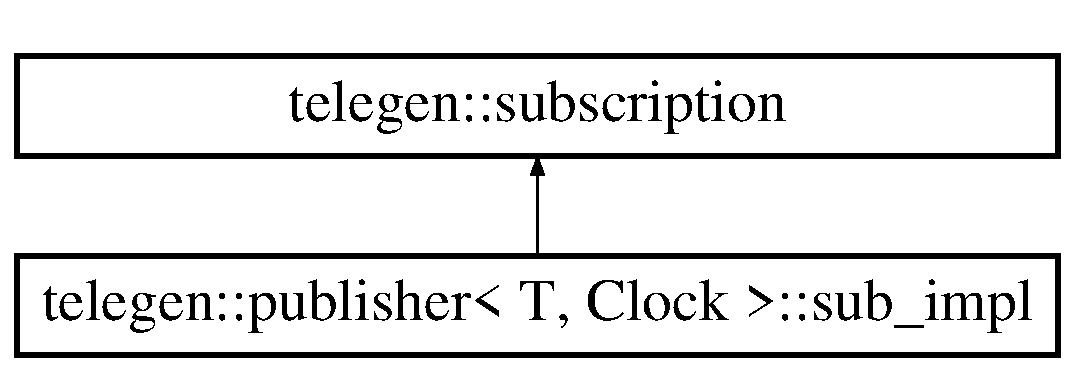
\includegraphics[height=2.000000cm]{classtelegen_1_1subscription}
\end{center}
\end{figure}
\subsection*{Public Member Functions}
\begin{DoxyCompactItemize}
\item 
\hyperlink{classtelegen_1_1subscription_a506c90eb0e3ba380473a742011ef3f3b}{subscription} (\hyperlink{namespacetelegen_ad925de2d0a99bc43918533abf0457344}{interval} min\+\_\+time, \hyperlink{namespacetelegen_ad925de2d0a99bc43918533abf0457344}{interval} max\+\_\+time)
\item 
virtual \hyperlink{classtelegen_1_1subscription_a2dcbdaadf0071d4f4485f018bceb7eb6}{$\sim$subscription} ()
\item 
virtual bool \hyperlink{classtelegen_1_1subscription_a4bbe4edbb2ecba3ccff4d6de562e2e7d}{is\+\_\+cancelled} ()=0
\item 
virtual \hyperlink{namespacetelegen_a9dd802bb5d30cf96b0c616750d43ae86}{promise} \hyperlink{classtelegen_1_1subscription_a7d645e1bf76477316d9f868a69467e42}{cancel} (\hyperlink{namespacetelegen_ad925de2d0a99bc43918533abf0457344}{interval} timeout)=0
\item 
virtual \hyperlink{namespacetelegen_a9dd802bb5d30cf96b0c616750d43ae86}{promise} \hyperlink{classtelegen_1_1subscription_aca992d1891107380ec81a517ea0bde58}{change} (\hyperlink{namespacetelegen_ad925de2d0a99bc43918533abf0457344}{interval} min\+\_\+interval, \hyperlink{namespacetelegen_ad925de2d0a99bc43918533abf0457344}{interval} max\+\_\+interval, \hyperlink{namespacetelegen_ad925de2d0a99bc43918533abf0457344}{interval} timeout)=0
\item 
constexpr \hyperlink{namespacetelegen_ad925de2d0a99bc43918533abf0457344}{interval} \hyperlink{classtelegen_1_1subscription_a81200099d915e3e69c0c1dbd940dfc40}{get\+\_\+min\+\_\+interval} () const
\item 
constexpr \hyperlink{namespacetelegen_ad925de2d0a99bc43918533abf0457344}{interval} \hyperlink{classtelegen_1_1subscription_a7901d4f487f0a8348a0593cd0787f7f9}{get\+\_\+max\+\_\+interval} () const
\item 
void \hyperlink{classtelegen_1_1subscription_acde1f5ed4c26f44c2b9f1929cf1af725}{handler} (const \hyperlink{classstdext_1_1inplace__function}{stdext\+::inplace\+\_\+function}$<$ void(const \hyperlink{classtelegen_1_1value}{value} \&), 16 $>$ \&cb)
\item 
void \hyperlink{classtelegen_1_1subscription_a84147a4afc90285df4c12d9243ffdece}{cancel\+\_\+handler} (const \hyperlink{classstdext_1_1inplace__function}{stdext\+::inplace\+\_\+function}$<$ void(), 16 $>$ \&cb)
\end{DoxyCompactItemize}
\subsection*{Protected Attributes}
\begin{DoxyCompactItemize}
\item 
\hyperlink{namespacetelegen_ad925de2d0a99bc43918533abf0457344}{interval} \hyperlink{classtelegen_1_1subscription_a6aee0684ec18cb68e68c7110742dc625}{min\+\_\+interval\+\_\+}
\item 
\hyperlink{namespacetelegen_ad925de2d0a99bc43918533abf0457344}{interval} \hyperlink{classtelegen_1_1subscription_afbf8aaf4fdfd91ef0f210ade501c04b1}{max\+\_\+interval\+\_\+}
\item 
\hyperlink{classstdext_1_1inplace__function}{stdext\+::inplace\+\_\+function}$<$ void(const \hyperlink{classtelegen_1_1value}{value} \&val), 16 $>$ \hyperlink{classtelegen_1_1subscription_a63b2db928cfeebed477b61b58b9a6446}{cb\+\_\+}
\item 
\hyperlink{classstdext_1_1inplace__function}{stdext\+::inplace\+\_\+function}$<$ void(), 16 $>$ \hyperlink{classtelegen_1_1subscription_aea82d071d3075d6b3ae8b36bf05f2d0e}{cancel\+\_\+cb\+\_\+}
\end{DoxyCompactItemize}


\subsection{Constructor \& Destructor Documentation}
\mbox{\Hypertarget{classtelegen_1_1subscription_a506c90eb0e3ba380473a742011ef3f3b}\label{classtelegen_1_1subscription_a506c90eb0e3ba380473a742011ef3f3b}} 
\index{telegen\+::subscription@{telegen\+::subscription}!subscription@{subscription}}
\index{subscription@{subscription}!telegen\+::subscription@{telegen\+::subscription}}
\subsubsection{\texorpdfstring{subscription()}{subscription()}}
{\footnotesize\ttfamily telegen\+::subscription\+::subscription (\begin{DoxyParamCaption}\item[{\hyperlink{namespacetelegen_ad925de2d0a99bc43918533abf0457344}{interval}}]{min\+\_\+time,  }\item[{\hyperlink{namespacetelegen_ad925de2d0a99bc43918533abf0457344}{interval}}]{max\+\_\+time }\end{DoxyParamCaption})\hspace{0.3cm}{\ttfamily [inline]}}

\mbox{\Hypertarget{classtelegen_1_1subscription_a2dcbdaadf0071d4f4485f018bceb7eb6}\label{classtelegen_1_1subscription_a2dcbdaadf0071d4f4485f018bceb7eb6}} 
\index{telegen\+::subscription@{telegen\+::subscription}!````~subscription@{$\sim$subscription}}
\index{````~subscription@{$\sim$subscription}!telegen\+::subscription@{telegen\+::subscription}}
\subsubsection{\texorpdfstring{$\sim$subscription()}{~subscription()}}
{\footnotesize\ttfamily virtual telegen\+::subscription\+::$\sim$subscription (\begin{DoxyParamCaption}{ }\end{DoxyParamCaption})\hspace{0.3cm}{\ttfamily [inline]}, {\ttfamily [virtual]}}



\subsection{Member Function Documentation}
\mbox{\Hypertarget{classtelegen_1_1subscription_a7d645e1bf76477316d9f868a69467e42}\label{classtelegen_1_1subscription_a7d645e1bf76477316d9f868a69467e42}} 
\index{telegen\+::subscription@{telegen\+::subscription}!cancel@{cancel}}
\index{cancel@{cancel}!telegen\+::subscription@{telegen\+::subscription}}
\subsubsection{\texorpdfstring{cancel()}{cancel()}}
{\footnotesize\ttfamily virtual \hyperlink{namespacetelegen_a9dd802bb5d30cf96b0c616750d43ae86}{promise} telegen\+::subscription\+::cancel (\begin{DoxyParamCaption}\item[{\hyperlink{namespacetelegen_ad925de2d0a99bc43918533abf0457344}{interval}}]{timeout }\end{DoxyParamCaption})\hspace{0.3cm}{\ttfamily [pure virtual]}}



Implemented in \hyperlink{classtelegen_1_1publisher_1_1sub__impl_ae0a84e8e0a45d21c688ee557c603c43d}{telegen\+::publisher$<$ T, Clock $>$\+::sub\+\_\+impl}.

\mbox{\Hypertarget{classtelegen_1_1subscription_a84147a4afc90285df4c12d9243ffdece}\label{classtelegen_1_1subscription_a84147a4afc90285df4c12d9243ffdece}} 
\index{telegen\+::subscription@{telegen\+::subscription}!cancel\+\_\+handler@{cancel\+\_\+handler}}
\index{cancel\+\_\+handler@{cancel\+\_\+handler}!telegen\+::subscription@{telegen\+::subscription}}
\subsubsection{\texorpdfstring{cancel\+\_\+handler()}{cancel\_handler()}}
{\footnotesize\ttfamily void telegen\+::subscription\+::cancel\+\_\+handler (\begin{DoxyParamCaption}\item[{const \hyperlink{classstdext_1_1inplace__function}{stdext\+::inplace\+\_\+function}$<$ void(), 16 $>$ \&}]{cb }\end{DoxyParamCaption})\hspace{0.3cm}{\ttfamily [inline]}}

\mbox{\Hypertarget{classtelegen_1_1subscription_aca992d1891107380ec81a517ea0bde58}\label{classtelegen_1_1subscription_aca992d1891107380ec81a517ea0bde58}} 
\index{telegen\+::subscription@{telegen\+::subscription}!change@{change}}
\index{change@{change}!telegen\+::subscription@{telegen\+::subscription}}
\subsubsection{\texorpdfstring{change()}{change()}}
{\footnotesize\ttfamily virtual \hyperlink{namespacetelegen_a9dd802bb5d30cf96b0c616750d43ae86}{promise} telegen\+::subscription\+::change (\begin{DoxyParamCaption}\item[{\hyperlink{namespacetelegen_ad925de2d0a99bc43918533abf0457344}{interval}}]{min\+\_\+interval,  }\item[{\hyperlink{namespacetelegen_ad925de2d0a99bc43918533abf0457344}{interval}}]{max\+\_\+interval,  }\item[{\hyperlink{namespacetelegen_ad925de2d0a99bc43918533abf0457344}{interval}}]{timeout }\end{DoxyParamCaption})\hspace{0.3cm}{\ttfamily [pure virtual]}}



Implemented in \hyperlink{classtelegen_1_1publisher_1_1sub__impl_a2144a27beee3ef15a21fb7fd323b3770}{telegen\+::publisher$<$ T, Clock $>$\+::sub\+\_\+impl}.

\mbox{\Hypertarget{classtelegen_1_1subscription_a7901d4f487f0a8348a0593cd0787f7f9}\label{classtelegen_1_1subscription_a7901d4f487f0a8348a0593cd0787f7f9}} 
\index{telegen\+::subscription@{telegen\+::subscription}!get\+\_\+max\+\_\+interval@{get\+\_\+max\+\_\+interval}}
\index{get\+\_\+max\+\_\+interval@{get\+\_\+max\+\_\+interval}!telegen\+::subscription@{telegen\+::subscription}}
\subsubsection{\texorpdfstring{get\+\_\+max\+\_\+interval()}{get\_max\_interval()}}
{\footnotesize\ttfamily constexpr \hyperlink{namespacetelegen_ad925de2d0a99bc43918533abf0457344}{interval} telegen\+::subscription\+::get\+\_\+max\+\_\+interval (\begin{DoxyParamCaption}{ }\end{DoxyParamCaption}) const\hspace{0.3cm}{\ttfamily [inline]}}

\mbox{\Hypertarget{classtelegen_1_1subscription_a81200099d915e3e69c0c1dbd940dfc40}\label{classtelegen_1_1subscription_a81200099d915e3e69c0c1dbd940dfc40}} 
\index{telegen\+::subscription@{telegen\+::subscription}!get\+\_\+min\+\_\+interval@{get\+\_\+min\+\_\+interval}}
\index{get\+\_\+min\+\_\+interval@{get\+\_\+min\+\_\+interval}!telegen\+::subscription@{telegen\+::subscription}}
\subsubsection{\texorpdfstring{get\+\_\+min\+\_\+interval()}{get\_min\_interval()}}
{\footnotesize\ttfamily constexpr \hyperlink{namespacetelegen_ad925de2d0a99bc43918533abf0457344}{interval} telegen\+::subscription\+::get\+\_\+min\+\_\+interval (\begin{DoxyParamCaption}{ }\end{DoxyParamCaption}) const\hspace{0.3cm}{\ttfamily [inline]}}

\mbox{\Hypertarget{classtelegen_1_1subscription_acde1f5ed4c26f44c2b9f1929cf1af725}\label{classtelegen_1_1subscription_acde1f5ed4c26f44c2b9f1929cf1af725}} 
\index{telegen\+::subscription@{telegen\+::subscription}!handler@{handler}}
\index{handler@{handler}!telegen\+::subscription@{telegen\+::subscription}}
\subsubsection{\texorpdfstring{handler()}{handler()}}
{\footnotesize\ttfamily void telegen\+::subscription\+::handler (\begin{DoxyParamCaption}\item[{const \hyperlink{classstdext_1_1inplace__function}{stdext\+::inplace\+\_\+function}$<$ void(const \hyperlink{classtelegen_1_1value}{value} \&), 16 $>$ \&}]{cb }\end{DoxyParamCaption})\hspace{0.3cm}{\ttfamily [inline]}}

\mbox{\Hypertarget{classtelegen_1_1subscription_a4bbe4edbb2ecba3ccff4d6de562e2e7d}\label{classtelegen_1_1subscription_a4bbe4edbb2ecba3ccff4d6de562e2e7d}} 
\index{telegen\+::subscription@{telegen\+::subscription}!is\+\_\+cancelled@{is\+\_\+cancelled}}
\index{is\+\_\+cancelled@{is\+\_\+cancelled}!telegen\+::subscription@{telegen\+::subscription}}
\subsubsection{\texorpdfstring{is\+\_\+cancelled()}{is\_cancelled()}}
{\footnotesize\ttfamily virtual bool telegen\+::subscription\+::is\+\_\+cancelled (\begin{DoxyParamCaption}{ }\end{DoxyParamCaption})\hspace{0.3cm}{\ttfamily [pure virtual]}}



Implemented in \hyperlink{classtelegen_1_1publisher_1_1sub__impl_a9880e80ac0b1887b5aec423abbc0a6f3}{telegen\+::publisher$<$ T, Clock $>$\+::sub\+\_\+impl}.



\subsection{Member Data Documentation}
\mbox{\Hypertarget{classtelegen_1_1subscription_aea82d071d3075d6b3ae8b36bf05f2d0e}\label{classtelegen_1_1subscription_aea82d071d3075d6b3ae8b36bf05f2d0e}} 
\index{telegen\+::subscription@{telegen\+::subscription}!cancel\+\_\+cb\+\_\+@{cancel\+\_\+cb\+\_\+}}
\index{cancel\+\_\+cb\+\_\+@{cancel\+\_\+cb\+\_\+}!telegen\+::subscription@{telegen\+::subscription}}
\subsubsection{\texorpdfstring{cancel\+\_\+cb\+\_\+}{cancel\_cb\_}}
{\footnotesize\ttfamily \hyperlink{classstdext_1_1inplace__function}{stdext\+::inplace\+\_\+function}$<$void(), 16$>$ telegen\+::subscription\+::cancel\+\_\+cb\+\_\+\hspace{0.3cm}{\ttfamily [protected]}}

\mbox{\Hypertarget{classtelegen_1_1subscription_a63b2db928cfeebed477b61b58b9a6446}\label{classtelegen_1_1subscription_a63b2db928cfeebed477b61b58b9a6446}} 
\index{telegen\+::subscription@{telegen\+::subscription}!cb\+\_\+@{cb\+\_\+}}
\index{cb\+\_\+@{cb\+\_\+}!telegen\+::subscription@{telegen\+::subscription}}
\subsubsection{\texorpdfstring{cb\+\_\+}{cb\_}}
{\footnotesize\ttfamily \hyperlink{classstdext_1_1inplace__function}{stdext\+::inplace\+\_\+function}$<$void(const \hyperlink{classtelegen_1_1value}{value}\& val), 16$>$ telegen\+::subscription\+::cb\+\_\+\hspace{0.3cm}{\ttfamily [protected]}}

\mbox{\Hypertarget{classtelegen_1_1subscription_afbf8aaf4fdfd91ef0f210ade501c04b1}\label{classtelegen_1_1subscription_afbf8aaf4fdfd91ef0f210ade501c04b1}} 
\index{telegen\+::subscription@{telegen\+::subscription}!max\+\_\+interval\+\_\+@{max\+\_\+interval\+\_\+}}
\index{max\+\_\+interval\+\_\+@{max\+\_\+interval\+\_\+}!telegen\+::subscription@{telegen\+::subscription}}
\subsubsection{\texorpdfstring{max\+\_\+interval\+\_\+}{max\_interval\_}}
{\footnotesize\ttfamily \hyperlink{namespacetelegen_ad925de2d0a99bc43918533abf0457344}{interval} telegen\+::subscription\+::max\+\_\+interval\+\_\+\hspace{0.3cm}{\ttfamily [protected]}}

\mbox{\Hypertarget{classtelegen_1_1subscription_a6aee0684ec18cb68e68c7110742dc625}\label{classtelegen_1_1subscription_a6aee0684ec18cb68e68c7110742dc625}} 
\index{telegen\+::subscription@{telegen\+::subscription}!min\+\_\+interval\+\_\+@{min\+\_\+interval\+\_\+}}
\index{min\+\_\+interval\+\_\+@{min\+\_\+interval\+\_\+}!telegen\+::subscription@{telegen\+::subscription}}
\subsubsection{\texorpdfstring{min\+\_\+interval\+\_\+}{min\_interval\_}}
{\footnotesize\ttfamily \hyperlink{namespacetelegen_ad925de2d0a99bc43918533abf0457344}{interval} telegen\+::subscription\+::min\+\_\+interval\+\_\+\hspace{0.3cm}{\ttfamily [protected]}}



The documentation for this class was generated from the following file\+:\begin{DoxyCompactItemize}
\item 
\hyperlink{gen_2telegen_2nodes_8hpp}{gen/telegen/nodes.\+hpp}\end{DoxyCompactItemize}

\hypertarget{structtelegraph_1_1generator_1_1target}{}\section{telegraph\+:\+:generator\+:\+:target Struct Reference}
\label{structtelegraph_1_1generator_1_1target}\index{telegraph\+::generator\+::target@{telegraph\+::generator\+::target}}


{\ttfamily \#include $<$generator.\+hpp$>$}

\subsection*{Public Member Functions}
\begin{DoxyCompactItemize}
\item 
\hyperlink{structtelegraph_1_1generator_1_1target_a99ead371ab5d5fa9a5d33ed38394cc8d}{target} ()
\end{DoxyCompactItemize}
\subsection*{Public Attributes}
\begin{DoxyCompactItemize}
\item 
std\+::string \hyperlink{structtelegraph_1_1generator_1_1target_afe5f00222e1bc22846632ec37614226f}{filename}
\item 
std\+::string \hyperlink{structtelegraph_1_1generator_1_1target_abcbb3fbc6891d3298dd5c1e5632dadfa}{name\+\_\+space}
\item 
std\+::string \hyperlink{structtelegraph_1_1generator_1_1target_aae55a691127405908abada75477f234a}{tree\+\_\+include}
\item 
const \hyperlink{classtelegraph_1_1node}{node} $\ast$ \hyperlink{structtelegraph_1_1generator_1_1target_acbc17bb4f9cf53165d08b55841364260}{tree\+\_\+target}
\item 
std\+::vector$<$ const \hyperlink{classtelegraph_1_1profile}{profile} $\ast$ $>$ \hyperlink{structtelegraph_1_1generator_1_1target_ab6790d8a369d72b032ad122d94b0beaf}{profiles}
\end{DoxyCompactItemize}


\subsection{Constructor \& Destructor Documentation}
\mbox{\Hypertarget{structtelegraph_1_1generator_1_1target_a99ead371ab5d5fa9a5d33ed38394cc8d}\label{structtelegraph_1_1generator_1_1target_a99ead371ab5d5fa9a5d33ed38394cc8d}} 
\index{telegraph\+::generator\+::target@{telegraph\+::generator\+::target}!target@{target}}
\index{target@{target}!telegraph\+::generator\+::target@{telegraph\+::generator\+::target}}
\subsubsection{\texorpdfstring{target()}{target()}}
{\footnotesize\ttfamily telegraph\+::generator\+::target\+::target (\begin{DoxyParamCaption}{ }\end{DoxyParamCaption})\hspace{0.3cm}{\ttfamily [inline]}}



\subsection{Member Data Documentation}
\mbox{\Hypertarget{structtelegraph_1_1generator_1_1target_afe5f00222e1bc22846632ec37614226f}\label{structtelegraph_1_1generator_1_1target_afe5f00222e1bc22846632ec37614226f}} 
\index{telegraph\+::generator\+::target@{telegraph\+::generator\+::target}!filename@{filename}}
\index{filename@{filename}!telegraph\+::generator\+::target@{telegraph\+::generator\+::target}}
\subsubsection{\texorpdfstring{filename}{filename}}
{\footnotesize\ttfamily std\+::string telegraph\+::generator\+::target\+::filename}

\mbox{\Hypertarget{structtelegraph_1_1generator_1_1target_abcbb3fbc6891d3298dd5c1e5632dadfa}\label{structtelegraph_1_1generator_1_1target_abcbb3fbc6891d3298dd5c1e5632dadfa}} 
\index{telegraph\+::generator\+::target@{telegraph\+::generator\+::target}!name\+\_\+space@{name\+\_\+space}}
\index{name\+\_\+space@{name\+\_\+space}!telegraph\+::generator\+::target@{telegraph\+::generator\+::target}}
\subsubsection{\texorpdfstring{name\+\_\+space}{name\_space}}
{\footnotesize\ttfamily std\+::string telegraph\+::generator\+::target\+::name\+\_\+space}

\mbox{\Hypertarget{structtelegraph_1_1generator_1_1target_ab6790d8a369d72b032ad122d94b0beaf}\label{structtelegraph_1_1generator_1_1target_ab6790d8a369d72b032ad122d94b0beaf}} 
\index{telegraph\+::generator\+::target@{telegraph\+::generator\+::target}!profiles@{profiles}}
\index{profiles@{profiles}!telegraph\+::generator\+::target@{telegraph\+::generator\+::target}}
\subsubsection{\texorpdfstring{profiles}{profiles}}
{\footnotesize\ttfamily std\+::vector$<$const \hyperlink{classtelegraph_1_1profile}{profile}$\ast$$>$ telegraph\+::generator\+::target\+::profiles}

\mbox{\Hypertarget{structtelegraph_1_1generator_1_1target_aae55a691127405908abada75477f234a}\label{structtelegraph_1_1generator_1_1target_aae55a691127405908abada75477f234a}} 
\index{telegraph\+::generator\+::target@{telegraph\+::generator\+::target}!tree\+\_\+include@{tree\+\_\+include}}
\index{tree\+\_\+include@{tree\+\_\+include}!telegraph\+::generator\+::target@{telegraph\+::generator\+::target}}
\subsubsection{\texorpdfstring{tree\+\_\+include}{tree\_include}}
{\footnotesize\ttfamily std\+::string telegraph\+::generator\+::target\+::tree\+\_\+include}

\mbox{\Hypertarget{structtelegraph_1_1generator_1_1target_acbc17bb4f9cf53165d08b55841364260}\label{structtelegraph_1_1generator_1_1target_acbc17bb4f9cf53165d08b55841364260}} 
\index{telegraph\+::generator\+::target@{telegraph\+::generator\+::target}!tree\+\_\+target@{tree\+\_\+target}}
\index{tree\+\_\+target@{tree\+\_\+target}!telegraph\+::generator\+::target@{telegraph\+::generator\+::target}}
\subsubsection{\texorpdfstring{tree\+\_\+target}{tree\_target}}
{\footnotesize\ttfamily const \hyperlink{classtelegraph_1_1node}{node}$\ast$ telegraph\+::generator\+::target\+::tree\+\_\+target}



The documentation for this struct was generated from the following file\+:\begin{DoxyCompactItemize}
\item 
\hyperlink{generator_8hpp}{generator.\+hpp}\end{DoxyCompactItemize}

\hypertarget{classtelegraph_1_1tmp__archive}{}\section{telegraph\+:\+:tmp\+\_\+archive Class Reference}
\label{classtelegraph_1_1tmp__archive}\index{telegraph\+::tmp\+\_\+archive@{telegraph\+::tmp\+\_\+archive}}


{\ttfamily \#include $<$tmp\+\_\+archive.\+hpp$>$}

Inheritance diagram for telegraph\+:\+:tmp\+\_\+archive\+:\begin{figure}[H]
\begin{center}
\leavevmode
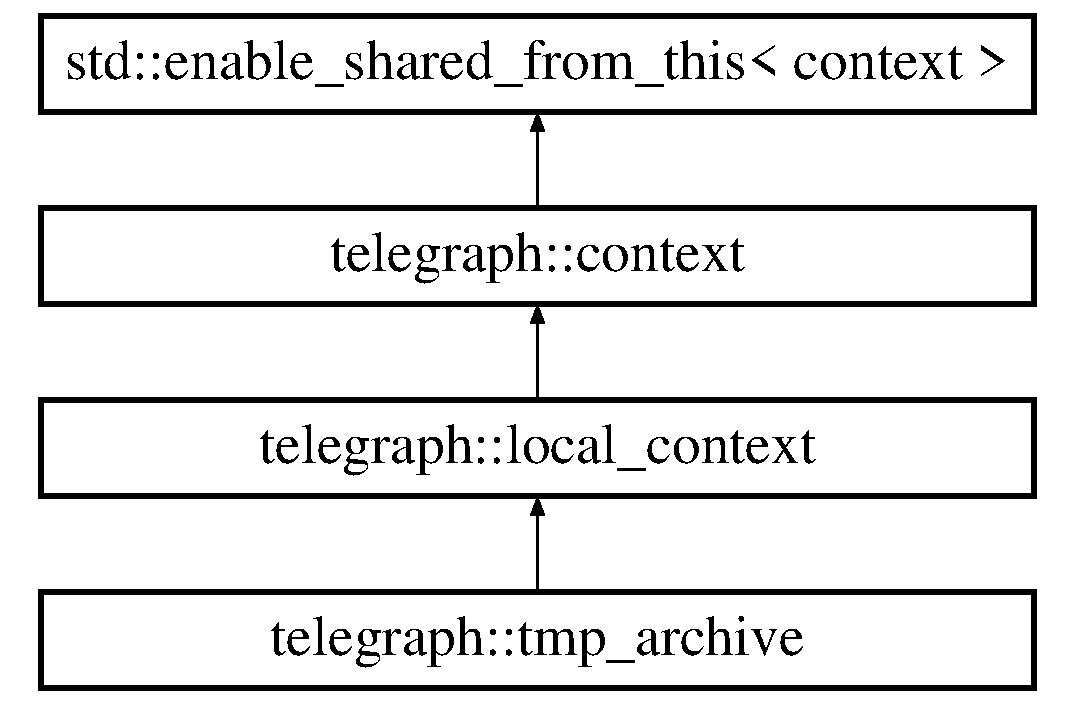
\includegraphics[height=4.000000cm]{classtelegraph_1_1tmp__archive}
\end{center}
\end{figure}
\subsection*{Public Member Functions}
\begin{DoxyCompactItemize}
\item 
\hyperlink{classtelegraph_1_1tmp__archive_a38157c35014a713c871fda88651c7318}{tmp\+\_\+archive} (io\+::io\+\_\+context \&ioc, const std\+::string\+\_\+view \&name, std\+::unique\+\_\+ptr$<$ \hyperlink{classtelegraph_1_1node}{node} $>$ \&\&s)
\item 
\hyperlink{classtelegraph_1_1tmp__archive_aef321341a53bb0ff5c0c3bd6df3290de}{$\sim$tmp\+\_\+archive} ()
\item 
\hyperlink{namespacetelegraph_ad071241508ea0f86c7de0686016f9ca9}{params\+\_\+stream\+\_\+ptr} \hyperlink{classtelegraph_1_1tmp__archive_a688a661b85092244e5634f9c3e380f94}{request} (\hyperlink{structboost_1_1asio_1_1yield__ctx}{io\+::yield\+\_\+ctx} \&, const \hyperlink{classtelegraph_1_1params}{params} \&p) override
\item 
void \hyperlink{classtelegraph_1_1tmp__archive_a6c71e7bf706d35c3e751e0bc7c8555b9}{record} (\hyperlink{classtelegraph_1_1variable}{variable} $\ast$v, \hyperlink{namespacetelegraph_a58641aa5b1a2cbdb0431916a87069f64}{subscription\+\_\+ptr} s)
\item 
void \hyperlink{classtelegraph_1_1tmp__archive_a92ecdf029db73b48ca0d7eaf2838a492}{record\+\_\+stop} (\hyperlink{classtelegraph_1_1variable}{variable} $\ast$v)
\item 
bool \hyperlink{classtelegraph_1_1tmp__archive_ae1838ff3fc3f1cd0eab31535a2f2e974}{write\+\_\+data} (\hyperlink{structboost_1_1asio_1_1yield__ctx}{io\+::yield\+\_\+ctx} \&yield, \hyperlink{classtelegraph_1_1variable}{variable} $\ast$v, const std\+::vector$<$ \hyperlink{classtelegraph_1_1data__point}{data\+\_\+point} $>$ \&data) override
\item 
bool \hyperlink{classtelegraph_1_1tmp__archive_a228c2c681beb749268d09cd83d594246}{write\+\_\+data} (\hyperlink{structboost_1_1asio_1_1yield__ctx}{io\+::yield\+\_\+ctx} \&yield, const std\+::vector$<$ std\+::string\+\_\+view $>$ \&v, const std\+::vector$<$ \hyperlink{classtelegraph_1_1data__point}{data\+\_\+point} $>$ \&data) override
\item 
\hyperlink{namespacetelegraph_a6ffe775ac48dca2a4013b53d692199c8}{data\+\_\+query\+\_\+ptr} \hyperlink{classtelegraph_1_1tmp__archive_a7f2d18d2a4c9a7fd65d9752c8f4ce4d5}{query\+\_\+data} (\hyperlink{structboost_1_1asio_1_1yield__ctx}{io\+::yield\+\_\+ctx} \&ctx, const \hyperlink{classtelegraph_1_1variable}{variable} $\ast$v) override
\item 
\hyperlink{namespacetelegraph_a6ffe775ac48dca2a4013b53d692199c8}{data\+\_\+query\+\_\+ptr} \hyperlink{classtelegraph_1_1tmp__archive_a8a860d67e3733e2eee7a8315942450e5}{query\+\_\+data} (\hyperlink{structboost_1_1asio_1_1yield__ctx}{io\+::yield\+\_\+ctx} \&ctx, const std\+::vector$<$ std\+::string\+\_\+view $>$ \&v) override
\item 
\hyperlink{namespacetelegraph_a58641aa5b1a2cbdb0431916a87069f64}{subscription\+\_\+ptr} \hyperlink{classtelegraph_1_1tmp__archive_a10adc383103f4183e0a37485a5406cf1}{subscribe} (\hyperlink{structboost_1_1asio_1_1yield__ctx}{io\+::yield\+\_\+ctx} \&ctx, const \hyperlink{classtelegraph_1_1variable}{variable} $\ast$v, float min\+\_\+interval, float max\+\_\+interval, float timeout) override
\item 
\hyperlink{namespacetelegraph_a58641aa5b1a2cbdb0431916a87069f64}{subscription\+\_\+ptr} \hyperlink{classtelegraph_1_1tmp__archive_a9cf4be673f860b875b085c1ecac913ff}{subscribe} (\hyperlink{structboost_1_1asio_1_1yield__ctx}{io\+::yield\+\_\+ctx} \&yield, const std\+::vector$<$ std\+::string\+\_\+view $>$ \&path, float min\+\_\+interval, float max\+\_\+interval, float timeout) override
\item 
\hyperlink{classtelegraph_1_1value}{value} \hyperlink{classtelegraph_1_1tmp__archive_a9edb8a731ef989f40ae06e4b6c63c0be}{call} (\hyperlink{structboost_1_1asio_1_1yield__ctx}{io\+::yield\+\_\+ctx} \&yield, \hyperlink{classtelegraph_1_1action}{action} $\ast$a, \hyperlink{classtelegraph_1_1value}{value} v, float timeout) override
\item 
\hyperlink{classtelegraph_1_1value}{value} \hyperlink{classtelegraph_1_1tmp__archive_a1ccf8c90f14b36f3a09a501e0931e42e}{call} (\hyperlink{structboost_1_1asio_1_1yield__ctx}{io\+::yield\+\_\+ctx} \&yield, const std\+::vector$<$ std\+::string\+\_\+view $>$ \&path, \hyperlink{classtelegraph_1_1value}{value} v, float timeout) override
\end{DoxyCompactItemize}
\subsection*{Static Public Member Functions}
\begin{DoxyCompactItemize}
\item 
static \hyperlink{namespacetelegraph_ab59c7b38d99a98b4acc22433c920b1e6}{local\+\_\+context\+\_\+ptr} \hyperlink{classtelegraph_1_1tmp__archive_a3e59e0a0a2ef78286399fd6f67b4431d}{create} (\hyperlink{structboost_1_1asio_1_1yield__ctx}{io\+::yield\+\_\+ctx} \&, io\+::io\+\_\+context \&ioc, const std\+::string\+\_\+view \&name, const std\+::string\+\_\+view \&type, const \hyperlink{classtelegraph_1_1params}{params} \&p)
\end{DoxyCompactItemize}
\subsection*{Additional Inherited Members}


\subsection{Constructor \& Destructor Documentation}
\mbox{\Hypertarget{classtelegraph_1_1tmp__archive_a38157c35014a713c871fda88651c7318}\label{classtelegraph_1_1tmp__archive_a38157c35014a713c871fda88651c7318}} 
\index{telegraph\+::tmp\+\_\+archive@{telegraph\+::tmp\+\_\+archive}!tmp\+\_\+archive@{tmp\+\_\+archive}}
\index{tmp\+\_\+archive@{tmp\+\_\+archive}!telegraph\+::tmp\+\_\+archive@{telegraph\+::tmp\+\_\+archive}}
\subsubsection{\texorpdfstring{tmp\+\_\+archive()}{tmp\_archive()}}
{\footnotesize\ttfamily telegraph\+::tmp\+\_\+archive\+::tmp\+\_\+archive (\begin{DoxyParamCaption}\item[{io\+::io\+\_\+context \&}]{ioc,  }\item[{const std\+::string\+\_\+view \&}]{name,  }\item[{std\+::unique\+\_\+ptr$<$ \hyperlink{classtelegraph_1_1node}{node} $>$ \&\&}]{s }\end{DoxyParamCaption})}

\mbox{\Hypertarget{classtelegraph_1_1tmp__archive_aef321341a53bb0ff5c0c3bd6df3290de}\label{classtelegraph_1_1tmp__archive_aef321341a53bb0ff5c0c3bd6df3290de}} 
\index{telegraph\+::tmp\+\_\+archive@{telegraph\+::tmp\+\_\+archive}!````~tmp\+\_\+archive@{$\sim$tmp\+\_\+archive}}
\index{````~tmp\+\_\+archive@{$\sim$tmp\+\_\+archive}!telegraph\+::tmp\+\_\+archive@{telegraph\+::tmp\+\_\+archive}}
\subsubsection{\texorpdfstring{$\sim$tmp\+\_\+archive()}{~tmp\_archive()}}
{\footnotesize\ttfamily telegraph\+::tmp\+\_\+archive\+::$\sim$tmp\+\_\+archive (\begin{DoxyParamCaption}{ }\end{DoxyParamCaption})}



\subsection{Member Function Documentation}
\mbox{\Hypertarget{classtelegraph_1_1tmp__archive_a9edb8a731ef989f40ae06e4b6c63c0be}\label{classtelegraph_1_1tmp__archive_a9edb8a731ef989f40ae06e4b6c63c0be}} 
\index{telegraph\+::tmp\+\_\+archive@{telegraph\+::tmp\+\_\+archive}!call@{call}}
\index{call@{call}!telegraph\+::tmp\+\_\+archive@{telegraph\+::tmp\+\_\+archive}}
\subsubsection{\texorpdfstring{call()}{call()}\hspace{0.1cm}{\footnotesize\ttfamily [1/2]}}
{\footnotesize\ttfamily \hyperlink{classtelegraph_1_1value}{value} telegraph\+::tmp\+\_\+archive\+::call (\begin{DoxyParamCaption}\item[{\hyperlink{structboost_1_1asio_1_1yield__ctx}{io\+::yield\+\_\+ctx} \&}]{yield,  }\item[{\hyperlink{classtelegraph_1_1action}{action} $\ast$}]{a,  }\item[{\hyperlink{classtelegraph_1_1value}{value}}]{v,  }\item[{float}]{timeout }\end{DoxyParamCaption})\hspace{0.3cm}{\ttfamily [inline]}, {\ttfamily [override]}, {\ttfamily [virtual]}}



Implements \hyperlink{classtelegraph_1_1context_a72da471eb635e5505b10d2f1103359ac}{telegraph\+::context}.

\mbox{\Hypertarget{classtelegraph_1_1tmp__archive_a1ccf8c90f14b36f3a09a501e0931e42e}\label{classtelegraph_1_1tmp__archive_a1ccf8c90f14b36f3a09a501e0931e42e}} 
\index{telegraph\+::tmp\+\_\+archive@{telegraph\+::tmp\+\_\+archive}!call@{call}}
\index{call@{call}!telegraph\+::tmp\+\_\+archive@{telegraph\+::tmp\+\_\+archive}}
\subsubsection{\texorpdfstring{call()}{call()}\hspace{0.1cm}{\footnotesize\ttfamily [2/2]}}
{\footnotesize\ttfamily \hyperlink{classtelegraph_1_1value}{value} telegraph\+::tmp\+\_\+archive\+::call (\begin{DoxyParamCaption}\item[{\hyperlink{structboost_1_1asio_1_1yield__ctx}{io\+::yield\+\_\+ctx} \&}]{yield,  }\item[{const std\+::vector$<$ std\+::string\+\_\+view $>$ \&}]{path,  }\item[{\hyperlink{classtelegraph_1_1value}{value}}]{v,  }\item[{float}]{timeout }\end{DoxyParamCaption})\hspace{0.3cm}{\ttfamily [inline]}, {\ttfamily [override]}, {\ttfamily [virtual]}}



Implements \hyperlink{classtelegraph_1_1context_a0798d49ea0874a870d4c980f6f09b6c2}{telegraph\+::context}.

\mbox{\Hypertarget{classtelegraph_1_1tmp__archive_a3e59e0a0a2ef78286399fd6f67b4431d}\label{classtelegraph_1_1tmp__archive_a3e59e0a0a2ef78286399fd6f67b4431d}} 
\index{telegraph\+::tmp\+\_\+archive@{telegraph\+::tmp\+\_\+archive}!create@{create}}
\index{create@{create}!telegraph\+::tmp\+\_\+archive@{telegraph\+::tmp\+\_\+archive}}
\subsubsection{\texorpdfstring{create()}{create()}}
{\footnotesize\ttfamily \hyperlink{namespacetelegraph_ab59c7b38d99a98b4acc22433c920b1e6}{local\+\_\+context\+\_\+ptr} telegraph\+::tmp\+\_\+archive\+::create (\begin{DoxyParamCaption}\item[{\hyperlink{structboost_1_1asio_1_1yield__ctx}{io\+::yield\+\_\+ctx} \&}]{yield,  }\item[{io\+::io\+\_\+context \&}]{ioc,  }\item[{const std\+::string\+\_\+view \&}]{name,  }\item[{const std\+::string\+\_\+view \&}]{type,  }\item[{const \hyperlink{classtelegraph_1_1params}{params} \&}]{p }\end{DoxyParamCaption})\hspace{0.3cm}{\ttfamily [static]}}

\mbox{\Hypertarget{classtelegraph_1_1tmp__archive_a7f2d18d2a4c9a7fd65d9752c8f4ce4d5}\label{classtelegraph_1_1tmp__archive_a7f2d18d2a4c9a7fd65d9752c8f4ce4d5}} 
\index{telegraph\+::tmp\+\_\+archive@{telegraph\+::tmp\+\_\+archive}!query\+\_\+data@{query\+\_\+data}}
\index{query\+\_\+data@{query\+\_\+data}!telegraph\+::tmp\+\_\+archive@{telegraph\+::tmp\+\_\+archive}}
\subsubsection{\texorpdfstring{query\+\_\+data()}{query\_data()}\hspace{0.1cm}{\footnotesize\ttfamily [1/2]}}
{\footnotesize\ttfamily \hyperlink{namespacetelegraph_a6ffe775ac48dca2a4013b53d692199c8}{data\+\_\+query\+\_\+ptr} telegraph\+::tmp\+\_\+archive\+::query\+\_\+data (\begin{DoxyParamCaption}\item[{\hyperlink{structboost_1_1asio_1_1yield__ctx}{io\+::yield\+\_\+ctx} \&}]{ctx,  }\item[{const \hyperlink{classtelegraph_1_1variable}{variable} $\ast$}]{v }\end{DoxyParamCaption})\hspace{0.3cm}{\ttfamily [inline]}, {\ttfamily [override]}, {\ttfamily [virtual]}}



Implements \hyperlink{classtelegraph_1_1context_a301114c9b73194507ae58221566a3e57}{telegraph\+::context}.

\mbox{\Hypertarget{classtelegraph_1_1tmp__archive_a8a860d67e3733e2eee7a8315942450e5}\label{classtelegraph_1_1tmp__archive_a8a860d67e3733e2eee7a8315942450e5}} 
\index{telegraph\+::tmp\+\_\+archive@{telegraph\+::tmp\+\_\+archive}!query\+\_\+data@{query\+\_\+data}}
\index{query\+\_\+data@{query\+\_\+data}!telegraph\+::tmp\+\_\+archive@{telegraph\+::tmp\+\_\+archive}}
\subsubsection{\texorpdfstring{query\+\_\+data()}{query\_data()}\hspace{0.1cm}{\footnotesize\ttfamily [2/2]}}
{\footnotesize\ttfamily \hyperlink{namespacetelegraph_a6ffe775ac48dca2a4013b53d692199c8}{data\+\_\+query\+\_\+ptr} telegraph\+::tmp\+\_\+archive\+::query\+\_\+data (\begin{DoxyParamCaption}\item[{\hyperlink{structboost_1_1asio_1_1yield__ctx}{io\+::yield\+\_\+ctx} \&}]{ctx,  }\item[{const std\+::vector$<$ std\+::string\+\_\+view $>$ \&}]{v }\end{DoxyParamCaption})\hspace{0.3cm}{\ttfamily [override]}, {\ttfamily [virtual]}}



Implements \hyperlink{classtelegraph_1_1context_a34793623d2a2def580ad0b8710c74c6d}{telegraph\+::context}.

\mbox{\Hypertarget{classtelegraph_1_1tmp__archive_a6c71e7bf706d35c3e751e0bc7c8555b9}\label{classtelegraph_1_1tmp__archive_a6c71e7bf706d35c3e751e0bc7c8555b9}} 
\index{telegraph\+::tmp\+\_\+archive@{telegraph\+::tmp\+\_\+archive}!record@{record}}
\index{record@{record}!telegraph\+::tmp\+\_\+archive@{telegraph\+::tmp\+\_\+archive}}
\subsubsection{\texorpdfstring{record()}{record()}}
{\footnotesize\ttfamily void telegraph\+::tmp\+\_\+archive\+::record (\begin{DoxyParamCaption}\item[{\hyperlink{classtelegraph_1_1variable}{variable} $\ast$}]{v,  }\item[{\hyperlink{namespacetelegraph_a58641aa5b1a2cbdb0431916a87069f64}{subscription\+\_\+ptr}}]{s }\end{DoxyParamCaption})}

\mbox{\Hypertarget{classtelegraph_1_1tmp__archive_a92ecdf029db73b48ca0d7eaf2838a492}\label{classtelegraph_1_1tmp__archive_a92ecdf029db73b48ca0d7eaf2838a492}} 
\index{telegraph\+::tmp\+\_\+archive@{telegraph\+::tmp\+\_\+archive}!record\+\_\+stop@{record\+\_\+stop}}
\index{record\+\_\+stop@{record\+\_\+stop}!telegraph\+::tmp\+\_\+archive@{telegraph\+::tmp\+\_\+archive}}
\subsubsection{\texorpdfstring{record\+\_\+stop()}{record\_stop()}}
{\footnotesize\ttfamily void telegraph\+::tmp\+\_\+archive\+::record\+\_\+stop (\begin{DoxyParamCaption}\item[{\hyperlink{classtelegraph_1_1variable}{variable} $\ast$}]{v }\end{DoxyParamCaption})}

\mbox{\Hypertarget{classtelegraph_1_1tmp__archive_a688a661b85092244e5634f9c3e380f94}\label{classtelegraph_1_1tmp__archive_a688a661b85092244e5634f9c3e380f94}} 
\index{telegraph\+::tmp\+\_\+archive@{telegraph\+::tmp\+\_\+archive}!request@{request}}
\index{request@{request}!telegraph\+::tmp\+\_\+archive@{telegraph\+::tmp\+\_\+archive}}
\subsubsection{\texorpdfstring{request()}{request()}}
{\footnotesize\ttfamily \hyperlink{namespacetelegraph_ad071241508ea0f86c7de0686016f9ca9}{params\+\_\+stream\+\_\+ptr} telegraph\+::tmp\+\_\+archive\+::request (\begin{DoxyParamCaption}\item[{\hyperlink{structboost_1_1asio_1_1yield__ctx}{io\+::yield\+\_\+ctx} \&}]{yield,  }\item[{const \hyperlink{classtelegraph_1_1params}{params} \&}]{p }\end{DoxyParamCaption})\hspace{0.3cm}{\ttfamily [override]}, {\ttfamily [virtual]}}



Implements \hyperlink{classtelegraph_1_1context_a6765d7fa22fe99b9a6723c511396b781}{telegraph\+::context}.

\mbox{\Hypertarget{classtelegraph_1_1tmp__archive_a10adc383103f4183e0a37485a5406cf1}\label{classtelegraph_1_1tmp__archive_a10adc383103f4183e0a37485a5406cf1}} 
\index{telegraph\+::tmp\+\_\+archive@{telegraph\+::tmp\+\_\+archive}!subscribe@{subscribe}}
\index{subscribe@{subscribe}!telegraph\+::tmp\+\_\+archive@{telegraph\+::tmp\+\_\+archive}}
\subsubsection{\texorpdfstring{subscribe()}{subscribe()}\hspace{0.1cm}{\footnotesize\ttfamily [1/2]}}
{\footnotesize\ttfamily \hyperlink{namespacetelegraph_a58641aa5b1a2cbdb0431916a87069f64}{subscription\+\_\+ptr} telegraph\+::tmp\+\_\+archive\+::subscribe (\begin{DoxyParamCaption}\item[{\hyperlink{structboost_1_1asio_1_1yield__ctx}{io\+::yield\+\_\+ctx} \&}]{ctx,  }\item[{const \hyperlink{classtelegraph_1_1variable}{variable} $\ast$}]{v,  }\item[{float}]{min\+\_\+interval,  }\item[{float}]{max\+\_\+interval,  }\item[{float}]{timeout }\end{DoxyParamCaption})\hspace{0.3cm}{\ttfamily [inline]}, {\ttfamily [override]}, {\ttfamily [virtual]}}



Implements \hyperlink{classtelegraph_1_1context_aec3b3b0d7210a86f2ea2f5067ef8e922}{telegraph\+::context}.

\mbox{\Hypertarget{classtelegraph_1_1tmp__archive_a9cf4be673f860b875b085c1ecac913ff}\label{classtelegraph_1_1tmp__archive_a9cf4be673f860b875b085c1ecac913ff}} 
\index{telegraph\+::tmp\+\_\+archive@{telegraph\+::tmp\+\_\+archive}!subscribe@{subscribe}}
\index{subscribe@{subscribe}!telegraph\+::tmp\+\_\+archive@{telegraph\+::tmp\+\_\+archive}}
\subsubsection{\texorpdfstring{subscribe()}{subscribe()}\hspace{0.1cm}{\footnotesize\ttfamily [2/2]}}
{\footnotesize\ttfamily \hyperlink{namespacetelegraph_a58641aa5b1a2cbdb0431916a87069f64}{subscription\+\_\+ptr} telegraph\+::tmp\+\_\+archive\+::subscribe (\begin{DoxyParamCaption}\item[{\hyperlink{structboost_1_1asio_1_1yield__ctx}{io\+::yield\+\_\+ctx} \&}]{yield,  }\item[{const std\+::vector$<$ std\+::string\+\_\+view $>$ \&}]{path,  }\item[{float}]{min\+\_\+interval,  }\item[{float}]{max\+\_\+interval,  }\item[{float}]{timeout }\end{DoxyParamCaption})\hspace{0.3cm}{\ttfamily [inline]}, {\ttfamily [override]}, {\ttfamily [virtual]}}



Implements \hyperlink{classtelegraph_1_1context_a8db167973f187f707a4108e112683969}{telegraph\+::context}.

\mbox{\Hypertarget{classtelegraph_1_1tmp__archive_ae1838ff3fc3f1cd0eab31535a2f2e974}\label{classtelegraph_1_1tmp__archive_ae1838ff3fc3f1cd0eab31535a2f2e974}} 
\index{telegraph\+::tmp\+\_\+archive@{telegraph\+::tmp\+\_\+archive}!write\+\_\+data@{write\+\_\+data}}
\index{write\+\_\+data@{write\+\_\+data}!telegraph\+::tmp\+\_\+archive@{telegraph\+::tmp\+\_\+archive}}
\subsubsection{\texorpdfstring{write\+\_\+data()}{write\_data()}\hspace{0.1cm}{\footnotesize\ttfamily [1/2]}}
{\footnotesize\ttfamily bool telegraph\+::tmp\+\_\+archive\+::write\+\_\+data (\begin{DoxyParamCaption}\item[{\hyperlink{structboost_1_1asio_1_1yield__ctx}{io\+::yield\+\_\+ctx} \&}]{yield,  }\item[{\hyperlink{classtelegraph_1_1variable}{variable} $\ast$}]{v,  }\item[{const std\+::vector$<$ \hyperlink{classtelegraph_1_1data__point}{data\+\_\+point} $>$ \&}]{data }\end{DoxyParamCaption})\hspace{0.3cm}{\ttfamily [inline]}, {\ttfamily [override]}, {\ttfamily [virtual]}}



Implements \hyperlink{classtelegraph_1_1context_a6067b9a6f2590733c81f6a3b2ed9cba7}{telegraph\+::context}.

\mbox{\Hypertarget{classtelegraph_1_1tmp__archive_a228c2c681beb749268d09cd83d594246}\label{classtelegraph_1_1tmp__archive_a228c2c681beb749268d09cd83d594246}} 
\index{telegraph\+::tmp\+\_\+archive@{telegraph\+::tmp\+\_\+archive}!write\+\_\+data@{write\+\_\+data}}
\index{write\+\_\+data@{write\+\_\+data}!telegraph\+::tmp\+\_\+archive@{telegraph\+::tmp\+\_\+archive}}
\subsubsection{\texorpdfstring{write\+\_\+data()}{write\_data()}\hspace{0.1cm}{\footnotesize\ttfamily [2/2]}}
{\footnotesize\ttfamily bool telegraph\+::tmp\+\_\+archive\+::write\+\_\+data (\begin{DoxyParamCaption}\item[{\hyperlink{structboost_1_1asio_1_1yield__ctx}{io\+::yield\+\_\+ctx} \&}]{yield,  }\item[{const std\+::vector$<$ std\+::string\+\_\+view $>$ \&}]{v,  }\item[{const std\+::vector$<$ \hyperlink{classtelegraph_1_1data__point}{data\+\_\+point} $>$ \&}]{data }\end{DoxyParamCaption})\hspace{0.3cm}{\ttfamily [inline]}, {\ttfamily [override]}, {\ttfamily [virtual]}}



Implements \hyperlink{classtelegraph_1_1context_a1f600d6159df21dd2750b1c706ca3412}{telegraph\+::context}.



The documentation for this class was generated from the following files\+:\begin{DoxyCompactItemize}
\item 
\hyperlink{tmp__archive_8hpp}{tmp\+\_\+archive.\+hpp}\item 
\hyperlink{tmp__archive_8cpp}{tmp\+\_\+archive.\+cpp}\end{DoxyCompactItemize}

\hypertarget{classtelegraph_1_1tmp__data}{}\section{telegraph\+:\+:tmp\+\_\+data Class Reference}
\label{classtelegraph_1_1tmp__data}\index{telegraph\+::tmp\+\_\+data@{telegraph\+::tmp\+\_\+data}}


{\ttfamily \#include $<$tmp\+\_\+archive.\+hpp$>$}

Inheritance diagram for telegraph\+:\+:tmp\+\_\+data\+:\begin{figure}[H]
\begin{center}
\leavevmode
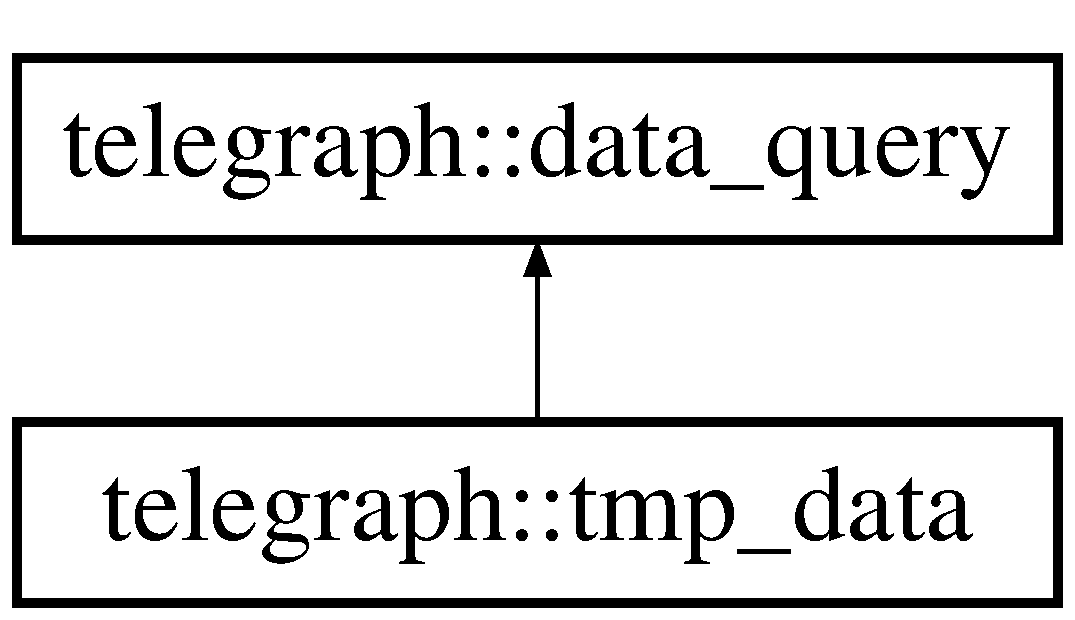
\includegraphics[height=2.000000cm]{classtelegraph_1_1tmp__data}
\end{center}
\end{figure}
\subsection*{Public Member Functions}
\begin{DoxyCompactItemize}
\item 
const std\+::vector$<$ \hyperlink{classtelegraph_1_1data__point}{data\+\_\+point} $>$ \& \hyperlink{classtelegraph_1_1tmp__data_a0cc69096544afeaffaae5f25587dc62f}{get\+\_\+current} () const override
\item 
void \hyperlink{classtelegraph_1_1tmp__data_a32f7e20afb889b3f9b179cfefed31f9e}{write} (const std\+::vector$<$ \hyperlink{classtelegraph_1_1data__point}{data\+\_\+point} $>$ \&d)
\end{DoxyCompactItemize}
\subsection*{Additional Inherited Members}


\subsection{Member Function Documentation}
\mbox{\Hypertarget{classtelegraph_1_1tmp__data_a0cc69096544afeaffaae5f25587dc62f}\label{classtelegraph_1_1tmp__data_a0cc69096544afeaffaae5f25587dc62f}} 
\index{telegraph\+::tmp\+\_\+data@{telegraph\+::tmp\+\_\+data}!get\+\_\+current@{get\+\_\+current}}
\index{get\+\_\+current@{get\+\_\+current}!telegraph\+::tmp\+\_\+data@{telegraph\+::tmp\+\_\+data}}
\subsubsection{\texorpdfstring{get\+\_\+current()}{get\_current()}}
{\footnotesize\ttfamily const std\+::vector$<$\hyperlink{classtelegraph_1_1data__point}{data\+\_\+point}$>$\& telegraph\+::tmp\+\_\+data\+::get\+\_\+current (\begin{DoxyParamCaption}{ }\end{DoxyParamCaption}) const\hspace{0.3cm}{\ttfamily [inline]}, {\ttfamily [override]}, {\ttfamily [virtual]}}



Implements \hyperlink{classtelegraph_1_1data__query_a20545e27166e025df2f73c13907bf721}{telegraph\+::data\+\_\+query}.

\mbox{\Hypertarget{classtelegraph_1_1tmp__data_a32f7e20afb889b3f9b179cfefed31f9e}\label{classtelegraph_1_1tmp__data_a32f7e20afb889b3f9b179cfefed31f9e}} 
\index{telegraph\+::tmp\+\_\+data@{telegraph\+::tmp\+\_\+data}!write@{write}}
\index{write@{write}!telegraph\+::tmp\+\_\+data@{telegraph\+::tmp\+\_\+data}}
\subsubsection{\texorpdfstring{write()}{write()}}
{\footnotesize\ttfamily void telegraph\+::tmp\+\_\+data\+::write (\begin{DoxyParamCaption}\item[{const std\+::vector$<$ \hyperlink{classtelegraph_1_1data__point}{data\+\_\+point} $>$ \&}]{d }\end{DoxyParamCaption})\hspace{0.3cm}{\ttfamily [inline]}}



The documentation for this class was generated from the following file\+:\begin{DoxyCompactItemize}
\item 
\hyperlink{tmp__archive_8hpp}{tmp\+\_\+archive.\+hpp}\end{DoxyCompactItemize}

\hypertarget{classtelegraph_1_1tree__error}{}\section{telegraph\+:\+:tree\+\_\+error Class Reference}
\label{classtelegraph_1_1tree__error}\index{telegraph\+::tree\+\_\+error@{telegraph\+::tree\+\_\+error}}


{\ttfamily \#include $<$errors.\+hpp$>$}

Inheritance diagram for telegraph\+:\+:tree\+\_\+error\+:\begin{figure}[H]
\begin{center}
\leavevmode
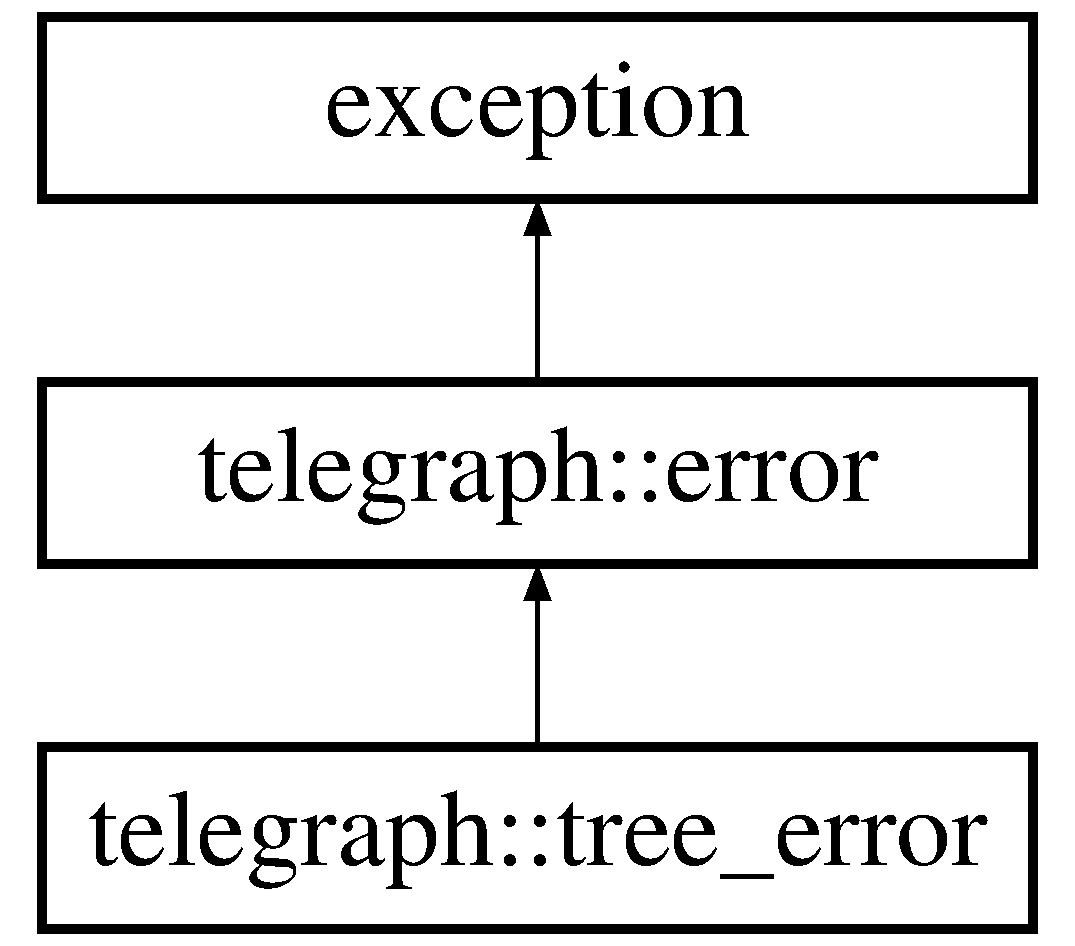
\includegraphics[height=3.000000cm]{classtelegraph_1_1tree__error}
\end{center}
\end{figure}
\subsection*{Public Member Functions}
\begin{DoxyCompactItemize}
\item 
\hyperlink{classtelegraph_1_1tree__error_a3700c5466473f44dd2001b74ceb97305}{tree\+\_\+error} (const std\+::string\+\_\+view \&m)
\end{DoxyCompactItemize}


\subsection{Constructor \& Destructor Documentation}
\mbox{\Hypertarget{classtelegraph_1_1tree__error_a3700c5466473f44dd2001b74ceb97305}\label{classtelegraph_1_1tree__error_a3700c5466473f44dd2001b74ceb97305}} 
\index{telegraph\+::tree\+\_\+error@{telegraph\+::tree\+\_\+error}!tree\+\_\+error@{tree\+\_\+error}}
\index{tree\+\_\+error@{tree\+\_\+error}!telegraph\+::tree\+\_\+error@{telegraph\+::tree\+\_\+error}}
\subsubsection{\texorpdfstring{tree\+\_\+error()}{tree\_error()}}
{\footnotesize\ttfamily telegraph\+::tree\+\_\+error\+::tree\+\_\+error (\begin{DoxyParamCaption}\item[{const std\+::string\+\_\+view \&}]{m }\end{DoxyParamCaption})\hspace{0.3cm}{\ttfamily [inline]}}



The documentation for this class was generated from the following file\+:\begin{DoxyCompactItemize}
\item 
\hyperlink{errors_8hpp}{errors.\+hpp}\end{DoxyCompactItemize}

\hypertarget{structtelegen_1_1type__info}{}\section{telegen\+:\+:type\+\_\+info$<$ T $>$ Struct Template Reference}
\label{structtelegen_1_1type__info}\index{telegen\+::type\+\_\+info$<$ T $>$@{telegen\+::type\+\_\+info$<$ T $>$}}


{\ttfamily \#include $<$types.\+hpp$>$}

\subsection*{Public Types}
\begin{DoxyCompactItemize}
\item 
using \hyperlink{structtelegen_1_1type__info_a9d062952fc241b6fd91df2b038995eaf}{value\+\_\+type} = T
\end{DoxyCompactItemize}
\subsection*{Public Member Functions}
\begin{DoxyCompactItemize}
\item 
constexpr \hyperlink{structtelegen_1_1type__info_a2f67a3b15149ac1a6a95354725f9d72a}{type\+\_\+info} (const char $\ast$nm, size\+\_\+t nl, const char $\ast$const $\ast$l)
\item 
void \hyperlink{structtelegen_1_1type__info_a5ed3d1c30970a84b6507c30890d74f86}{pack} (telegraph\+\_\+\+Type $\ast$type) const
\end{DoxyCompactItemize}
\subsection*{Public Attributes}
\begin{DoxyCompactItemize}
\item 
\hyperlink{namespacetelegen_a72d4e69f0be1731e1a851a96dec858d8}{type\+\_\+class} \hyperlink{structtelegen_1_1type__info_a7b45b05aeac67bd7700d3b140455f77f}{class\+\_\+}
\item 
const char $\ast$ \hyperlink{structtelegen_1_1type__info_ad2de0d0c01346808ffb8f86dfb4a3a0e}{name}
\item 
uint8\+\_\+t \hyperlink{structtelegen_1_1type__info_aada1921511a38c6889fe0d89701ce125}{num\+\_\+labels}
\item 
const char $\ast$const  $\ast$ \hyperlink{structtelegen_1_1type__info_a57e2f47e182fd9099f09ac086fd88be8}{labels}
\end{DoxyCompactItemize}


\subsection{Member Typedef Documentation}
\mbox{\Hypertarget{structtelegen_1_1type__info_a9d062952fc241b6fd91df2b038995eaf}\label{structtelegen_1_1type__info_a9d062952fc241b6fd91df2b038995eaf}} 
\index{telegen\+::type\+\_\+info@{telegen\+::type\+\_\+info}!value\+\_\+type@{value\+\_\+type}}
\index{value\+\_\+type@{value\+\_\+type}!telegen\+::type\+\_\+info@{telegen\+::type\+\_\+info}}
\subsubsection{\texorpdfstring{value\+\_\+type}{value\_type}}
{\footnotesize\ttfamily template$<$typename T$>$ \\
using \hyperlink{structtelegen_1_1type__info}{telegen\+::type\+\_\+info}$<$ T $>$\+::\hyperlink{structtelegen_1_1type__info_a9d062952fc241b6fd91df2b038995eaf}{value\+\_\+type} =  T}



\subsection{Constructor \& Destructor Documentation}
\mbox{\Hypertarget{structtelegen_1_1type__info_a2f67a3b15149ac1a6a95354725f9d72a}\label{structtelegen_1_1type__info_a2f67a3b15149ac1a6a95354725f9d72a}} 
\index{telegen\+::type\+\_\+info@{telegen\+::type\+\_\+info}!type\+\_\+info@{type\+\_\+info}}
\index{type\+\_\+info@{type\+\_\+info}!telegen\+::type\+\_\+info@{telegen\+::type\+\_\+info}}
\subsubsection{\texorpdfstring{type\+\_\+info()}{type\_info()}}
{\footnotesize\ttfamily template$<$typename T$>$ \\
constexpr \hyperlink{structtelegen_1_1type__info}{telegen\+::type\+\_\+info}$<$ T $>$\+::\hyperlink{structtelegen_1_1type__info}{type\+\_\+info} (\begin{DoxyParamCaption}\item[{const char $\ast$}]{nm,  }\item[{size\+\_\+t}]{nl,  }\item[{const char $\ast$const $\ast$}]{l }\end{DoxyParamCaption})\hspace{0.3cm}{\ttfamily [inline]}}



\subsection{Member Function Documentation}
\mbox{\Hypertarget{structtelegen_1_1type__info_a5ed3d1c30970a84b6507c30890d74f86}\label{structtelegen_1_1type__info_a5ed3d1c30970a84b6507c30890d74f86}} 
\index{telegen\+::type\+\_\+info@{telegen\+::type\+\_\+info}!pack@{pack}}
\index{pack@{pack}!telegen\+::type\+\_\+info@{telegen\+::type\+\_\+info}}
\subsubsection{\texorpdfstring{pack()}{pack()}}
{\footnotesize\ttfamily template$<$typename T$>$ \\
void \hyperlink{structtelegen_1_1type__info}{telegen\+::type\+\_\+info}$<$ T $>$\+::pack (\begin{DoxyParamCaption}\item[{telegraph\+\_\+\+Type $\ast$}]{type }\end{DoxyParamCaption}) const\hspace{0.3cm}{\ttfamily [inline]}}



\subsection{Member Data Documentation}
\mbox{\Hypertarget{structtelegen_1_1type__info_a7b45b05aeac67bd7700d3b140455f77f}\label{structtelegen_1_1type__info_a7b45b05aeac67bd7700d3b140455f77f}} 
\index{telegen\+::type\+\_\+info@{telegen\+::type\+\_\+info}!class\+\_\+@{class\+\_\+}}
\index{class\+\_\+@{class\+\_\+}!telegen\+::type\+\_\+info@{telegen\+::type\+\_\+info}}
\subsubsection{\texorpdfstring{class\+\_\+}{class\_}}
{\footnotesize\ttfamily template$<$typename T$>$ \\
\hyperlink{namespacetelegen_a72d4e69f0be1731e1a851a96dec858d8}{type\+\_\+class} \hyperlink{structtelegen_1_1type__info}{telegen\+::type\+\_\+info}$<$ T $>$\+::class\+\_\+}

\mbox{\Hypertarget{structtelegen_1_1type__info_a57e2f47e182fd9099f09ac086fd88be8}\label{structtelegen_1_1type__info_a57e2f47e182fd9099f09ac086fd88be8}} 
\index{telegen\+::type\+\_\+info@{telegen\+::type\+\_\+info}!labels@{labels}}
\index{labels@{labels}!telegen\+::type\+\_\+info@{telegen\+::type\+\_\+info}}
\subsubsection{\texorpdfstring{labels}{labels}}
{\footnotesize\ttfamily template$<$typename T$>$ \\
const char$\ast$ const$\ast$ \hyperlink{structtelegen_1_1type__info}{telegen\+::type\+\_\+info}$<$ T $>$\+::labels}

\mbox{\Hypertarget{structtelegen_1_1type__info_ad2de0d0c01346808ffb8f86dfb4a3a0e}\label{structtelegen_1_1type__info_ad2de0d0c01346808ffb8f86dfb4a3a0e}} 
\index{telegen\+::type\+\_\+info@{telegen\+::type\+\_\+info}!name@{name}}
\index{name@{name}!telegen\+::type\+\_\+info@{telegen\+::type\+\_\+info}}
\subsubsection{\texorpdfstring{name}{name}}
{\footnotesize\ttfamily template$<$typename T$>$ \\
const char$\ast$ \hyperlink{structtelegen_1_1type__info}{telegen\+::type\+\_\+info}$<$ T $>$\+::name}

\mbox{\Hypertarget{structtelegen_1_1type__info_aada1921511a38c6889fe0d89701ce125}\label{structtelegen_1_1type__info_aada1921511a38c6889fe0d89701ce125}} 
\index{telegen\+::type\+\_\+info@{telegen\+::type\+\_\+info}!num\+\_\+labels@{num\+\_\+labels}}
\index{num\+\_\+labels@{num\+\_\+labels}!telegen\+::type\+\_\+info@{telegen\+::type\+\_\+info}}
\subsubsection{\texorpdfstring{num\+\_\+labels}{num\_labels}}
{\footnotesize\ttfamily template$<$typename T$>$ \\
uint8\+\_\+t \hyperlink{structtelegen_1_1type__info}{telegen\+::type\+\_\+info}$<$ T $>$\+::num\+\_\+labels}



The documentation for this struct was generated from the following file\+:\begin{DoxyCompactItemize}
\item 
\hyperlink{types_8hpp}{types.\+hpp}\end{DoxyCompactItemize}

\hypertarget{classtelegen_1_1uart__interface}{}\section{telegen\+:\+:uart\+\_\+interface$<$ Uart, Clock $>$ Class Template Reference}
\label{classtelegen_1_1uart__interface}\index{telegen\+::uart\+\_\+interface$<$ Uart, Clock $>$@{telegen\+::uart\+\_\+interface$<$ Uart, Clock $>$}}


{\ttfamily \#include $<$uart\+\_\+interface.\+hpp$>$}

Inheritance diagram for telegen\+:\+:uart\+\_\+interface$<$ Uart, Clock $>$\+:\begin{figure}[H]
\begin{center}
\leavevmode
\includegraphics[height=2.000000cm]{classtelegen_1_1uart__interface}
\end{center}
\end{figure}
\subsection*{Public Member Functions}
\begin{DoxyCompactItemize}
\item 
\hyperlink{classtelegen_1_1uart__interface_a94948855fab15839bd7af6325b7de8ab}{uart\+\_\+interface} (Uart $\ast$u, Clock $\ast$c, \hyperlink{classtelegen_1_1node}{node} $\ast$root, \hyperlink{classtelegen_1_1node}{node} $\ast$const $\ast$id\+\_\+lookup\+\_\+table, size\+\_\+t table\+\_\+size, uint32\+\_\+t timeout)
\item 
\hyperlink{classtelegen_1_1uart__interface_a32429e63defd2d534b5d881eeff8c35c}{$\sim$uart\+\_\+interface} ()
\item 
\hyperlink{namespacetelegen_a9dd802bb5d30cf96b0c616750d43ae86}{promise}$<$ \hyperlink{namespacetelegen_a27c822534a5231fe1c523c81e8768afb}{subscription\+\_\+ptr} $>$ \hyperlink{classtelegen_1_1uart__interface_a869d06375865913880cf9818150c5b6e}{subscribe} (\hyperlink{classtelegen_1_1variable__base}{variable\+\_\+base} $\ast$v, \hyperlink{namespacetelegen_ad925de2d0a99bc43918533abf0457344}{interval} debounce, \hyperlink{namespacetelegen_ad925de2d0a99bc43918533abf0457344}{interval} referesh, \hyperlink{namespacetelegen_ad925de2d0a99bc43918533abf0457344}{interval} timeout) override
\item 
\hyperlink{namespacetelegen_a9dd802bb5d30cf96b0c616750d43ae86}{promise}$<$ \hyperlink{classtelegen_1_1value}{value} $>$ \hyperlink{classtelegen_1_1uart__interface_acaf4ff8f9442b3d4d2b9d5bcc252d08e}{call} (\hyperlink{classtelegen_1_1action__base}{action\+\_\+base} $\ast$a, \hyperlink{classtelegen_1_1value}{value} arg, \hyperlink{namespacetelegen_ad925de2d0a99bc43918533abf0457344}{interval} timeout) override
\item 
void \hyperlink{classtelegen_1_1uart__interface_a4552980fe3db33e65c631c785fa7b743}{notify\+\_\+success} (uint32\+\_\+t req\+\_\+id, bool success)
\item 
void \hyperlink{classtelegen_1_1uart__interface_a62a2abc8dd84e273c18e4d6f123253dc}{notify\+\_\+cancelled} (\hyperlink{classtelegen_1_1node_aae3ff0d12932c55fdc88a1743e27ea56}{node\+::id} var\+\_\+id)
\item 
void \hyperlink{classtelegen_1_1uart__interface_a27ccf80b5783baaa49300f27f061bd9f}{push\+\_\+update} (\hyperlink{classtelegen_1_1node_aae3ff0d12932c55fdc88a1743e27ea56}{node\+::id} var\+\_\+id, const \hyperlink{classtelegen_1_1value}{value} \&v)
\item 
void \hyperlink{classtelegen_1_1uart__interface_a7b7a2f161f41a0bea021876ba459c910}{received\+\_\+packet} (const telegraph\+\_\+stream\+\_\+\+Packet \&packet)
\item 
void \hyperlink{classtelegen_1_1uart__interface_af9ddca9952736ea442f0324cac0c1087}{write\+\_\+packet} (const telegraph\+\_\+stream\+\_\+\+Packet \&packet)
\item 
void \hyperlink{classtelegen_1_1uart__interface_a83061b24c65c0c50d89635af69fb1172}{reset\+\_\+read\+\_\+buf} ()
\item 
void \hyperlink{classtelegen_1_1uart__interface_ac126173cdd9ffe15a33e248dc3e8c2fc}{receive} ()
\item 
void \hyperlink{classtelegen_1_1uart__interface_acc4f7dbff9e17b04a55ece5f447272df}{resume} () override
\end{DoxyCompactItemize}


\subsection{Detailed Description}
\subsubsection*{template$<$typename Uart, typename Clock$>$\newline
class telegen\+::uart\+\_\+interface$<$ Uart, Clock $>$}

A stream interface is designed to be used on a bidirectional stream like a uart device

This is templated on the i/o stream class type and the timer type so that it can be reused for different platforms, each of which can implement their own stream/timer type (and so maximize performance by templating it) 

\subsection{Constructor \& Destructor Documentation}
\mbox{\Hypertarget{classtelegen_1_1uart__interface_a94948855fab15839bd7af6325b7de8ab}\label{classtelegen_1_1uart__interface_a94948855fab15839bd7af6325b7de8ab}} 
\index{telegen\+::uart\+\_\+interface@{telegen\+::uart\+\_\+interface}!uart\+\_\+interface@{uart\+\_\+interface}}
\index{uart\+\_\+interface@{uart\+\_\+interface}!telegen\+::uart\+\_\+interface@{telegen\+::uart\+\_\+interface}}
\subsubsection{\texorpdfstring{uart\+\_\+interface()}{uart\_interface()}}
{\footnotesize\ttfamily template$<$typename Uart , typename Clock $>$ \\
\hyperlink{classtelegen_1_1uart__interface}{telegen\+::uart\+\_\+interface}$<$ Uart, Clock $>$\+::\hyperlink{classtelegen_1_1uart__interface}{uart\+\_\+interface} (\begin{DoxyParamCaption}\item[{Uart $\ast$}]{u,  }\item[{Clock $\ast$}]{c,  }\item[{\hyperlink{classtelegen_1_1node}{node} $\ast$}]{root,  }\item[{\hyperlink{classtelegen_1_1node}{node} $\ast$const $\ast$}]{id\+\_\+lookup\+\_\+table,  }\item[{size\+\_\+t}]{table\+\_\+size,  }\item[{uint32\+\_\+t}]{timeout }\end{DoxyParamCaption})\hspace{0.3cm}{\ttfamily [inline]}}

\mbox{\Hypertarget{classtelegen_1_1uart__interface_a32429e63defd2d534b5d881eeff8c35c}\label{classtelegen_1_1uart__interface_a32429e63defd2d534b5d881eeff8c35c}} 
\index{telegen\+::uart\+\_\+interface@{telegen\+::uart\+\_\+interface}!````~uart\+\_\+interface@{$\sim$uart\+\_\+interface}}
\index{````~uart\+\_\+interface@{$\sim$uart\+\_\+interface}!telegen\+::uart\+\_\+interface@{telegen\+::uart\+\_\+interface}}
\subsubsection{\texorpdfstring{$\sim$uart\+\_\+interface()}{~uart\_interface()}}
{\footnotesize\ttfamily template$<$typename Uart , typename Clock $>$ \\
\hyperlink{classtelegen_1_1uart__interface}{telegen\+::uart\+\_\+interface}$<$ Uart, Clock $>$\+::$\sim$\hyperlink{classtelegen_1_1uart__interface}{uart\+\_\+interface} (\begin{DoxyParamCaption}{ }\end{DoxyParamCaption})\hspace{0.3cm}{\ttfamily [inline]}}



\subsection{Member Function Documentation}
\mbox{\Hypertarget{classtelegen_1_1uart__interface_acaf4ff8f9442b3d4d2b9d5bcc252d08e}\label{classtelegen_1_1uart__interface_acaf4ff8f9442b3d4d2b9d5bcc252d08e}} 
\index{telegen\+::uart\+\_\+interface@{telegen\+::uart\+\_\+interface}!call@{call}}
\index{call@{call}!telegen\+::uart\+\_\+interface@{telegen\+::uart\+\_\+interface}}
\subsubsection{\texorpdfstring{call()}{call()}}
{\footnotesize\ttfamily template$<$typename Uart , typename Clock $>$ \\
\hyperlink{namespacetelegen_a9dd802bb5d30cf96b0c616750d43ae86}{promise}$<$\hyperlink{classtelegen_1_1value}{value}$>$ \hyperlink{classtelegen_1_1uart__interface}{telegen\+::uart\+\_\+interface}$<$ Uart, Clock $>$\+::call (\begin{DoxyParamCaption}\item[{\hyperlink{classtelegen_1_1action__base}{action\+\_\+base} $\ast$}]{a,  }\item[{\hyperlink{classtelegen_1_1value}{value}}]{arg,  }\item[{\hyperlink{namespacetelegen_ad925de2d0a99bc43918533abf0457344}{interval}}]{timeout }\end{DoxyParamCaption})\hspace{0.3cm}{\ttfamily [inline]}, {\ttfamily [override]}, {\ttfamily [virtual]}}



Implements \hyperlink{classtelegen_1_1source_ae14191b0e6aa10521bb3d8fa5e1747e9}{telegen\+::source}.

\mbox{\Hypertarget{classtelegen_1_1uart__interface_a62a2abc8dd84e273c18e4d6f123253dc}\label{classtelegen_1_1uart__interface_a62a2abc8dd84e273c18e4d6f123253dc}} 
\index{telegen\+::uart\+\_\+interface@{telegen\+::uart\+\_\+interface}!notify\+\_\+cancelled@{notify\+\_\+cancelled}}
\index{notify\+\_\+cancelled@{notify\+\_\+cancelled}!telegen\+::uart\+\_\+interface@{telegen\+::uart\+\_\+interface}}
\subsubsection{\texorpdfstring{notify\+\_\+cancelled()}{notify\_cancelled()}}
{\footnotesize\ttfamily template$<$typename Uart , typename Clock $>$ \\
void \hyperlink{classtelegen_1_1uart__interface}{telegen\+::uart\+\_\+interface}$<$ Uart, Clock $>$\+::notify\+\_\+cancelled (\begin{DoxyParamCaption}\item[{\hyperlink{classtelegen_1_1node_aae3ff0d12932c55fdc88a1743e27ea56}{node\+::id}}]{var\+\_\+id }\end{DoxyParamCaption})\hspace{0.3cm}{\ttfamily [inline]}}

\mbox{\Hypertarget{classtelegen_1_1uart__interface_a4552980fe3db33e65c631c785fa7b743}\label{classtelegen_1_1uart__interface_a4552980fe3db33e65c631c785fa7b743}} 
\index{telegen\+::uart\+\_\+interface@{telegen\+::uart\+\_\+interface}!notify\+\_\+success@{notify\+\_\+success}}
\index{notify\+\_\+success@{notify\+\_\+success}!telegen\+::uart\+\_\+interface@{telegen\+::uart\+\_\+interface}}
\subsubsection{\texorpdfstring{notify\+\_\+success()}{notify\_success()}}
{\footnotesize\ttfamily template$<$typename Uart , typename Clock $>$ \\
void \hyperlink{classtelegen_1_1uart__interface}{telegen\+::uart\+\_\+interface}$<$ Uart, Clock $>$\+::notify\+\_\+success (\begin{DoxyParamCaption}\item[{uint32\+\_\+t}]{req\+\_\+id,  }\item[{bool}]{success }\end{DoxyParamCaption})\hspace{0.3cm}{\ttfamily [inline]}}

\mbox{\Hypertarget{classtelegen_1_1uart__interface_a27ccf80b5783baaa49300f27f061bd9f}\label{classtelegen_1_1uart__interface_a27ccf80b5783baaa49300f27f061bd9f}} 
\index{telegen\+::uart\+\_\+interface@{telegen\+::uart\+\_\+interface}!push\+\_\+update@{push\+\_\+update}}
\index{push\+\_\+update@{push\+\_\+update}!telegen\+::uart\+\_\+interface@{telegen\+::uart\+\_\+interface}}
\subsubsection{\texorpdfstring{push\+\_\+update()}{push\_update()}}
{\footnotesize\ttfamily template$<$typename Uart , typename Clock $>$ \\
void \hyperlink{classtelegen_1_1uart__interface}{telegen\+::uart\+\_\+interface}$<$ Uart, Clock $>$\+::push\+\_\+update (\begin{DoxyParamCaption}\item[{\hyperlink{classtelegen_1_1node_aae3ff0d12932c55fdc88a1743e27ea56}{node\+::id}}]{var\+\_\+id,  }\item[{const \hyperlink{classtelegen_1_1value}{value} \&}]{v }\end{DoxyParamCaption})\hspace{0.3cm}{\ttfamily [inline]}}

\mbox{\Hypertarget{classtelegen_1_1uart__interface_ac126173cdd9ffe15a33e248dc3e8c2fc}\label{classtelegen_1_1uart__interface_ac126173cdd9ffe15a33e248dc3e8c2fc}} 
\index{telegen\+::uart\+\_\+interface@{telegen\+::uart\+\_\+interface}!receive@{receive}}
\index{receive@{receive}!telegen\+::uart\+\_\+interface@{telegen\+::uart\+\_\+interface}}
\subsubsection{\texorpdfstring{receive()}{receive()}}
{\footnotesize\ttfamily template$<$typename Uart , typename Clock $>$ \\
void \hyperlink{classtelegen_1_1uart__interface}{telegen\+::uart\+\_\+interface}$<$ Uart, Clock $>$\+::receive (\begin{DoxyParamCaption}{ }\end{DoxyParamCaption})\hspace{0.3cm}{\ttfamily [inline]}}

\mbox{\Hypertarget{classtelegen_1_1uart__interface_a7b7a2f161f41a0bea021876ba459c910}\label{classtelegen_1_1uart__interface_a7b7a2f161f41a0bea021876ba459c910}} 
\index{telegen\+::uart\+\_\+interface@{telegen\+::uart\+\_\+interface}!received\+\_\+packet@{received\+\_\+packet}}
\index{received\+\_\+packet@{received\+\_\+packet}!telegen\+::uart\+\_\+interface@{telegen\+::uart\+\_\+interface}}
\subsubsection{\texorpdfstring{received\+\_\+packet()}{received\_packet()}}
{\footnotesize\ttfamily template$<$typename Uart , typename Clock $>$ \\
void \hyperlink{classtelegen_1_1uart__interface}{telegen\+::uart\+\_\+interface}$<$ Uart, Clock $>$\+::received\+\_\+packet (\begin{DoxyParamCaption}\item[{const telegraph\+\_\+stream\+\_\+\+Packet \&}]{packet }\end{DoxyParamCaption})\hspace{0.3cm}{\ttfamily [inline]}}

\mbox{\Hypertarget{classtelegen_1_1uart__interface_a83061b24c65c0c50d89635af69fb1172}\label{classtelegen_1_1uart__interface_a83061b24c65c0c50d89635af69fb1172}} 
\index{telegen\+::uart\+\_\+interface@{telegen\+::uart\+\_\+interface}!reset\+\_\+read\+\_\+buf@{reset\+\_\+read\+\_\+buf}}
\index{reset\+\_\+read\+\_\+buf@{reset\+\_\+read\+\_\+buf}!telegen\+::uart\+\_\+interface@{telegen\+::uart\+\_\+interface}}
\subsubsection{\texorpdfstring{reset\+\_\+read\+\_\+buf()}{reset\_read\_buf()}}
{\footnotesize\ttfamily template$<$typename Uart , typename Clock $>$ \\
void \hyperlink{classtelegen_1_1uart__interface}{telegen\+::uart\+\_\+interface}$<$ Uart, Clock $>$\+::reset\+\_\+read\+\_\+buf (\begin{DoxyParamCaption}{ }\end{DoxyParamCaption})\hspace{0.3cm}{\ttfamily [inline]}}

\mbox{\Hypertarget{classtelegen_1_1uart__interface_acc4f7dbff9e17b04a55ece5f447272df}\label{classtelegen_1_1uart__interface_acc4f7dbff9e17b04a55ece5f447272df}} 
\index{telegen\+::uart\+\_\+interface@{telegen\+::uart\+\_\+interface}!resume@{resume}}
\index{resume@{resume}!telegen\+::uart\+\_\+interface@{telegen\+::uart\+\_\+interface}}
\subsubsection{\texorpdfstring{resume()}{resume()}}
{\footnotesize\ttfamily template$<$typename Uart , typename Clock $>$ \\
void \hyperlink{classtelegen_1_1uart__interface}{telegen\+::uart\+\_\+interface}$<$ Uart, Clock $>$\+::resume (\begin{DoxyParamCaption}{ }\end{DoxyParamCaption})\hspace{0.3cm}{\ttfamily [inline]}, {\ttfamily [override]}, {\ttfamily [virtual]}}



Implements \hyperlink{structtelegen_1_1coroutine_a2a7408a5b9474af3e59128934e3a5c00}{telegen\+::coroutine}.

\mbox{\Hypertarget{classtelegen_1_1uart__interface_a869d06375865913880cf9818150c5b6e}\label{classtelegen_1_1uart__interface_a869d06375865913880cf9818150c5b6e}} 
\index{telegen\+::uart\+\_\+interface@{telegen\+::uart\+\_\+interface}!subscribe@{subscribe}}
\index{subscribe@{subscribe}!telegen\+::uart\+\_\+interface@{telegen\+::uart\+\_\+interface}}
\subsubsection{\texorpdfstring{subscribe()}{subscribe()}}
{\footnotesize\ttfamily template$<$typename Uart , typename Clock $>$ \\
\hyperlink{namespacetelegen_a9dd802bb5d30cf96b0c616750d43ae86}{promise}$<$\hyperlink{namespacetelegen_a27c822534a5231fe1c523c81e8768afb}{subscription\+\_\+ptr}$>$ \hyperlink{classtelegen_1_1uart__interface}{telegen\+::uart\+\_\+interface}$<$ Uart, Clock $>$\+::subscribe (\begin{DoxyParamCaption}\item[{\hyperlink{classtelegen_1_1variable__base}{variable\+\_\+base} $\ast$}]{v,  }\item[{\hyperlink{namespacetelegen_ad925de2d0a99bc43918533abf0457344}{interval}}]{debounce,  }\item[{\hyperlink{namespacetelegen_ad925de2d0a99bc43918533abf0457344}{interval}}]{referesh,  }\item[{\hyperlink{namespacetelegen_ad925de2d0a99bc43918533abf0457344}{interval}}]{timeout }\end{DoxyParamCaption})\hspace{0.3cm}{\ttfamily [inline]}, {\ttfamily [override]}, {\ttfamily [virtual]}}



Implements \hyperlink{classtelegen_1_1source_a224b4eb02ea346aca099615a5ae00ea9}{telegen\+::source}.

\mbox{\Hypertarget{classtelegen_1_1uart__interface_af9ddca9952736ea442f0324cac0c1087}\label{classtelegen_1_1uart__interface_af9ddca9952736ea442f0324cac0c1087}} 
\index{telegen\+::uart\+\_\+interface@{telegen\+::uart\+\_\+interface}!write\+\_\+packet@{write\+\_\+packet}}
\index{write\+\_\+packet@{write\+\_\+packet}!telegen\+::uart\+\_\+interface@{telegen\+::uart\+\_\+interface}}
\subsubsection{\texorpdfstring{write\+\_\+packet()}{write\_packet()}}
{\footnotesize\ttfamily template$<$typename Uart , typename Clock $>$ \\
void \hyperlink{classtelegen_1_1uart__interface}{telegen\+::uart\+\_\+interface}$<$ Uart, Clock $>$\+::write\+\_\+packet (\begin{DoxyParamCaption}\item[{const telegraph\+\_\+stream\+\_\+\+Packet \&}]{packet }\end{DoxyParamCaption})\hspace{0.3cm}{\ttfamily [inline]}}



The documentation for this class was generated from the following file\+:\begin{DoxyCompactItemize}
\item 
\hyperlink{uart__interface_8hpp}{uart\+\_\+interface.\+hpp}\end{DoxyCompactItemize}

\hypertarget{classtelegen_1_1value}{}\section{telegen\+:\+:value Class Reference}
\label{classtelegen_1_1value}\index{telegen\+::value@{telegen\+::value}}


{\ttfamily \#include $<$value.\+hpp$>$}

\subsection*{Classes}
\begin{DoxyCompactItemize}
\item 
union \hyperlink{uniontelegen_1_1value_1_1box}{box}
\end{DoxyCompactItemize}
\subsection*{Public Member Functions}
\begin{DoxyCompactItemize}
\item 
constexpr \hyperlink{classtelegen_1_1value_aa2c76dda3f9812dd9a031a0b463a6f5c}{value} ()
\item 
constexpr \hyperlink{classtelegen_1_1value_a7e501fb7a6f3b724255b88572a76d073}{value} (\hyperlink{namespacetelegen_a72d4e69f0be1731e1a851a96dec858d8}{type\+\_\+class} t)
\item 
constexpr \hyperlink{namespacetelegen_a72d4e69f0be1731e1a851a96dec858d8}{type\+\_\+class} \hyperlink{classtelegen_1_1value_a792839f18c1e787e369d3362f022362c}{get\+\_\+type\+\_\+class} () const
\item 
constexpr const \hyperlink{uniontelegen_1_1value_1_1box}{box} \& \hyperlink{classtelegen_1_1value_a28195c2d95fc3d7c61bcc32cb4f64d66}{get\+\_\+box} () const
\item 
constexpr \hyperlink{uniontelegen_1_1value_1_1box}{box} \& \hyperlink{classtelegen_1_1value_a81c1fb26319a11335d1745fc2d01e36b}{get\+\_\+box} ()
\item 
{\footnotesize template$<$typename T $>$ }\\constexpr const T \& \hyperlink{classtelegen_1_1value_a4bcd8e8317c0395b523596e4c0fa180d}{get} () const
\item 
{\footnotesize template$<$typename T $>$ }\\constexpr T \& \hyperlink{classtelegen_1_1value_af3cd1843daaccaadcdf2a526147c485e}{get} ()
\item 
{\footnotesize template$<$typename T $>$ }\\constexpr void \hyperlink{classtelegen_1_1value_a801da4870cd04e737db817d10fe6780c}{set} (const T \&v)
\item 
void \hyperlink{classtelegen_1_1value_a9bba0ce74da6b87a86dac99d0e5efa0c}{pack} (telegraph\+\_\+\+Value $\ast$val) const
\end{DoxyCompactItemize}


\subsection{Constructor \& Destructor Documentation}
\mbox{\Hypertarget{classtelegen_1_1value_aa2c76dda3f9812dd9a031a0b463a6f5c}\label{classtelegen_1_1value_aa2c76dda3f9812dd9a031a0b463a6f5c}} 
\index{telegen\+::value@{telegen\+::value}!value@{value}}
\index{value@{value}!telegen\+::value@{telegen\+::value}}
\subsubsection{\texorpdfstring{value()}{value()}\hspace{0.1cm}{\footnotesize\ttfamily [1/2]}}
{\footnotesize\ttfamily constexpr telegen\+::value\+::value (\begin{DoxyParamCaption}{ }\end{DoxyParamCaption})\hspace{0.3cm}{\ttfamily [inline]}}

\mbox{\Hypertarget{classtelegen_1_1value_a7e501fb7a6f3b724255b88572a76d073}\label{classtelegen_1_1value_a7e501fb7a6f3b724255b88572a76d073}} 
\index{telegen\+::value@{telegen\+::value}!value@{value}}
\index{value@{value}!telegen\+::value@{telegen\+::value}}
\subsubsection{\texorpdfstring{value()}{value()}\hspace{0.1cm}{\footnotesize\ttfamily [2/2]}}
{\footnotesize\ttfamily constexpr telegen\+::value\+::value (\begin{DoxyParamCaption}\item[{\hyperlink{namespacetelegen_a72d4e69f0be1731e1a851a96dec858d8}{type\+\_\+class}}]{t }\end{DoxyParamCaption})\hspace{0.3cm}{\ttfamily [inline]}}



\subsection{Member Function Documentation}
\mbox{\Hypertarget{classtelegen_1_1value_a4bcd8e8317c0395b523596e4c0fa180d}\label{classtelegen_1_1value_a4bcd8e8317c0395b523596e4c0fa180d}} 
\index{telegen\+::value@{telegen\+::value}!get@{get}}
\index{get@{get}!telegen\+::value@{telegen\+::value}}
\subsubsection{\texorpdfstring{get()}{get()}\hspace{0.1cm}{\footnotesize\ttfamily [1/2]}}
{\footnotesize\ttfamily template$<$typename T $>$ \\
constexpr const T\& telegen\+::value\+::get (\begin{DoxyParamCaption}{ }\end{DoxyParamCaption}) const\hspace{0.3cm}{\ttfamily [inline]}}

\mbox{\Hypertarget{classtelegen_1_1value_af3cd1843daaccaadcdf2a526147c485e}\label{classtelegen_1_1value_af3cd1843daaccaadcdf2a526147c485e}} 
\index{telegen\+::value@{telegen\+::value}!get@{get}}
\index{get@{get}!telegen\+::value@{telegen\+::value}}
\subsubsection{\texorpdfstring{get()}{get()}\hspace{0.1cm}{\footnotesize\ttfamily [2/2]}}
{\footnotesize\ttfamily template$<$typename T $>$ \\
constexpr T\& telegen\+::value\+::get (\begin{DoxyParamCaption}{ }\end{DoxyParamCaption})\hspace{0.3cm}{\ttfamily [inline]}}

\mbox{\Hypertarget{classtelegen_1_1value_a28195c2d95fc3d7c61bcc32cb4f64d66}\label{classtelegen_1_1value_a28195c2d95fc3d7c61bcc32cb4f64d66}} 
\index{telegen\+::value@{telegen\+::value}!get\+\_\+box@{get\+\_\+box}}
\index{get\+\_\+box@{get\+\_\+box}!telegen\+::value@{telegen\+::value}}
\subsubsection{\texorpdfstring{get\+\_\+box()}{get\_box()}\hspace{0.1cm}{\footnotesize\ttfamily [1/2]}}
{\footnotesize\ttfamily constexpr const \hyperlink{uniontelegen_1_1value_1_1box}{box}\& telegen\+::value\+::get\+\_\+box (\begin{DoxyParamCaption}{ }\end{DoxyParamCaption}) const\hspace{0.3cm}{\ttfamily [inline]}}

\mbox{\Hypertarget{classtelegen_1_1value_a81c1fb26319a11335d1745fc2d01e36b}\label{classtelegen_1_1value_a81c1fb26319a11335d1745fc2d01e36b}} 
\index{telegen\+::value@{telegen\+::value}!get\+\_\+box@{get\+\_\+box}}
\index{get\+\_\+box@{get\+\_\+box}!telegen\+::value@{telegen\+::value}}
\subsubsection{\texorpdfstring{get\+\_\+box()}{get\_box()}\hspace{0.1cm}{\footnotesize\ttfamily [2/2]}}
{\footnotesize\ttfamily constexpr \hyperlink{uniontelegen_1_1value_1_1box}{box}\& telegen\+::value\+::get\+\_\+box (\begin{DoxyParamCaption}{ }\end{DoxyParamCaption})\hspace{0.3cm}{\ttfamily [inline]}}

\mbox{\Hypertarget{classtelegen_1_1value_a792839f18c1e787e369d3362f022362c}\label{classtelegen_1_1value_a792839f18c1e787e369d3362f022362c}} 
\index{telegen\+::value@{telegen\+::value}!get\+\_\+type\+\_\+class@{get\+\_\+type\+\_\+class}}
\index{get\+\_\+type\+\_\+class@{get\+\_\+type\+\_\+class}!telegen\+::value@{telegen\+::value}}
\subsubsection{\texorpdfstring{get\+\_\+type\+\_\+class()}{get\_type\_class()}}
{\footnotesize\ttfamily constexpr \hyperlink{namespacetelegen_a72d4e69f0be1731e1a851a96dec858d8}{type\+\_\+class} telegen\+::value\+::get\+\_\+type\+\_\+class (\begin{DoxyParamCaption}{ }\end{DoxyParamCaption}) const\hspace{0.3cm}{\ttfamily [inline]}}

\mbox{\Hypertarget{classtelegen_1_1value_a9bba0ce74da6b87a86dac99d0e5efa0c}\label{classtelegen_1_1value_a9bba0ce74da6b87a86dac99d0e5efa0c}} 
\index{telegen\+::value@{telegen\+::value}!pack@{pack}}
\index{pack@{pack}!telegen\+::value@{telegen\+::value}}
\subsubsection{\texorpdfstring{pack()}{pack()}}
{\footnotesize\ttfamily void telegen\+::value\+::pack (\begin{DoxyParamCaption}\item[{telegraph\+\_\+\+Value $\ast$}]{val }\end{DoxyParamCaption}) const\hspace{0.3cm}{\ttfamily [inline]}}

\mbox{\Hypertarget{classtelegen_1_1value_a801da4870cd04e737db817d10fe6780c}\label{classtelegen_1_1value_a801da4870cd04e737db817d10fe6780c}} 
\index{telegen\+::value@{telegen\+::value}!set@{set}}
\index{set@{set}!telegen\+::value@{telegen\+::value}}
\subsubsection{\texorpdfstring{set()}{set()}}
{\footnotesize\ttfamily template$<$typename T $>$ \\
constexpr void telegen\+::value\+::set (\begin{DoxyParamCaption}\item[{const T \&}]{v }\end{DoxyParamCaption})\hspace{0.3cm}{\ttfamily [inline]}}



The documentation for this class was generated from the following file\+:\begin{DoxyCompactItemize}
\item 
\hyperlink{gen_2telegen_2value_8hpp}{gen/telegen/value.\+hpp}\end{DoxyCompactItemize}

\hypertarget{classtelegraph_1_1value}{}\section{telegraph\+:\+:value Class Reference}
\label{classtelegraph_1_1value}\index{telegraph\+::value@{telegraph\+::value}}


{\ttfamily \#include $<$value.\+hpp$>$}

\subsection*{Classes}
\begin{DoxyCompactItemize}
\item 
union \hyperlink{uniontelegraph_1_1value_1_1box}{box}
\end{DoxyCompactItemize}
\subsection*{Public Member Functions}
\begin{DoxyCompactItemize}
\item 
constexpr \hyperlink{classtelegraph_1_1value_a0d68e7b123903adee0527771007ef9bb}{value} ()
\item 
constexpr \hyperlink{classtelegraph_1_1value_acdf151d4a74fc89dbf713b6a3bc010e7}{value} (bool b)
\item 
constexpr \hyperlink{classtelegraph_1_1value_ad60a01207482efd28cdfbe9d38618d44}{value} (uint8\+\_\+t v)
\item 
constexpr \hyperlink{classtelegraph_1_1value_a5d635c910bd217cbd8bf44a9ad92b8d6}{value} (uint16\+\_\+t v)
\item 
constexpr \hyperlink{classtelegraph_1_1value_ab893e01cc0191c29681122e70febf0eb}{value} (uint32\+\_\+t v)
\item 
constexpr \hyperlink{classtelegraph_1_1value_a74a4b302ca334adb99eac3e14e2cc9f0}{value} (uint64\+\_\+t v)
\item 
constexpr \hyperlink{classtelegraph_1_1value_abec206177d942003c27a025c5b430649}{value} (int8\+\_\+t v)
\item 
constexpr \hyperlink{classtelegraph_1_1value_a79305dd1e9fcc13a7059b9605642ce2b}{value} (int16\+\_\+t v)
\item 
constexpr \hyperlink{classtelegraph_1_1value_ac6e027b6a9687c477ae78c19aa35935a}{value} (int32\+\_\+t v)
\item 
constexpr \hyperlink{classtelegraph_1_1value_abfa29a624716fa98577f810fc96c0f87}{value} (int64\+\_\+t v)
\item 
constexpr \hyperlink{classtelegraph_1_1value_ac0ec66475ec076cf9f7a76e0a5b804d4}{value} (float v)
\item 
constexpr \hyperlink{classtelegraph_1_1value_af0ad714556beb9cac21b887c4e67055f}{value} (double v)
\item 
constexpr \hyperlink{classtelegraph_1_1value_ad96b01fa30ad481c4695df1d06e9aa12}{value} (\hyperlink{classtelegraph_1_1value__type_a516081c0a4e231cb22554f48f052ff6f}{value\+\_\+type\+::type\+\_\+class} t, uint8\+\_\+t v)
\item 
\hyperlink{classtelegraph_1_1value_a3fad9e2214835f095af02feb1f91c49a}{value} (const Value \&v)
\item 
constexpr \hyperlink{classtelegraph_1_1value__type_a516081c0a4e231cb22554f48f052ff6f}{value\+\_\+type\+::type\+\_\+class} \hyperlink{classtelegraph_1_1value_ae38e5de94d5cfad919efe224da5a6c7d}{get\+\_\+type\+\_\+class} () const
\item 
constexpr const \hyperlink{uniontelegraph_1_1value_1_1box}{box} \& \hyperlink{classtelegraph_1_1value_a79d73fbd3e172c33f11fdf7fead2b97a}{get\+\_\+box} () const
\item 
constexpr bool \hyperlink{classtelegraph_1_1value_ad37d892925ba112c70d6c090c3623dd2}{is\+\_\+valid} ()
\item 
{\footnotesize template$<$typename T $>$ }\\T \hyperlink{classtelegraph_1_1value_a201fca0737b8be3128f2770b41087540}{get} () const
\item 
void \hyperlink{classtelegraph_1_1value_abc2188de92998eb93f801780370c56da}{pack} (Value $\ast$v)
\end{DoxyCompactItemize}
\subsection*{Static Public Member Functions}
\begin{DoxyCompactItemize}
\item 
static \hyperlink{classtelegraph_1_1value}{value} \hyperlink{classtelegraph_1_1value_a68b0f771058facdf968ff62de354b881}{invalid} ()
\item 
static \hyperlink{classtelegraph_1_1value}{value} \hyperlink{classtelegraph_1_1value_a3ca25fc3c78659ae5f29da61b2583e2c}{none} ()
\item 
static \hyperlink{classtelegraph_1_1value}{value} \hyperlink{classtelegraph_1_1value_abe64620f91527a2b36310c4ace2a2790}{unpack} (const Value \&v)
\end{DoxyCompactItemize}


\subsection{Constructor \& Destructor Documentation}
\mbox{\Hypertarget{classtelegraph_1_1value_a0d68e7b123903adee0527771007ef9bb}\label{classtelegraph_1_1value_a0d68e7b123903adee0527771007ef9bb}} 
\index{telegraph\+::value@{telegraph\+::value}!value@{value}}
\index{value@{value}!telegraph\+::value@{telegraph\+::value}}
\subsubsection{\texorpdfstring{value()}{value()}\hspace{0.1cm}{\footnotesize\ttfamily [1/14]}}
{\footnotesize\ttfamily constexpr telegraph\+::value\+::value (\begin{DoxyParamCaption}{ }\end{DoxyParamCaption})\hspace{0.3cm}{\ttfamily [inline]}}

\mbox{\Hypertarget{classtelegraph_1_1value_acdf151d4a74fc89dbf713b6a3bc010e7}\label{classtelegraph_1_1value_acdf151d4a74fc89dbf713b6a3bc010e7}} 
\index{telegraph\+::value@{telegraph\+::value}!value@{value}}
\index{value@{value}!telegraph\+::value@{telegraph\+::value}}
\subsubsection{\texorpdfstring{value()}{value()}\hspace{0.1cm}{\footnotesize\ttfamily [2/14]}}
{\footnotesize\ttfamily constexpr telegraph\+::value\+::value (\begin{DoxyParamCaption}\item[{bool}]{b }\end{DoxyParamCaption})\hspace{0.3cm}{\ttfamily [inline]}}

\mbox{\Hypertarget{classtelegraph_1_1value_ad60a01207482efd28cdfbe9d38618d44}\label{classtelegraph_1_1value_ad60a01207482efd28cdfbe9d38618d44}} 
\index{telegraph\+::value@{telegraph\+::value}!value@{value}}
\index{value@{value}!telegraph\+::value@{telegraph\+::value}}
\subsubsection{\texorpdfstring{value()}{value()}\hspace{0.1cm}{\footnotesize\ttfamily [3/14]}}
{\footnotesize\ttfamily constexpr telegraph\+::value\+::value (\begin{DoxyParamCaption}\item[{uint8\+\_\+t}]{v }\end{DoxyParamCaption})\hspace{0.3cm}{\ttfamily [inline]}}

\mbox{\Hypertarget{classtelegraph_1_1value_a5d635c910bd217cbd8bf44a9ad92b8d6}\label{classtelegraph_1_1value_a5d635c910bd217cbd8bf44a9ad92b8d6}} 
\index{telegraph\+::value@{telegraph\+::value}!value@{value}}
\index{value@{value}!telegraph\+::value@{telegraph\+::value}}
\subsubsection{\texorpdfstring{value()}{value()}\hspace{0.1cm}{\footnotesize\ttfamily [4/14]}}
{\footnotesize\ttfamily constexpr telegraph\+::value\+::value (\begin{DoxyParamCaption}\item[{uint16\+\_\+t}]{v }\end{DoxyParamCaption})\hspace{0.3cm}{\ttfamily [inline]}}

\mbox{\Hypertarget{classtelegraph_1_1value_ab893e01cc0191c29681122e70febf0eb}\label{classtelegraph_1_1value_ab893e01cc0191c29681122e70febf0eb}} 
\index{telegraph\+::value@{telegraph\+::value}!value@{value}}
\index{value@{value}!telegraph\+::value@{telegraph\+::value}}
\subsubsection{\texorpdfstring{value()}{value()}\hspace{0.1cm}{\footnotesize\ttfamily [5/14]}}
{\footnotesize\ttfamily constexpr telegraph\+::value\+::value (\begin{DoxyParamCaption}\item[{uint32\+\_\+t}]{v }\end{DoxyParamCaption})\hspace{0.3cm}{\ttfamily [inline]}}

\mbox{\Hypertarget{classtelegraph_1_1value_a74a4b302ca334adb99eac3e14e2cc9f0}\label{classtelegraph_1_1value_a74a4b302ca334adb99eac3e14e2cc9f0}} 
\index{telegraph\+::value@{telegraph\+::value}!value@{value}}
\index{value@{value}!telegraph\+::value@{telegraph\+::value}}
\subsubsection{\texorpdfstring{value()}{value()}\hspace{0.1cm}{\footnotesize\ttfamily [6/14]}}
{\footnotesize\ttfamily constexpr telegraph\+::value\+::value (\begin{DoxyParamCaption}\item[{uint64\+\_\+t}]{v }\end{DoxyParamCaption})\hspace{0.3cm}{\ttfamily [inline]}}

\mbox{\Hypertarget{classtelegraph_1_1value_abec206177d942003c27a025c5b430649}\label{classtelegraph_1_1value_abec206177d942003c27a025c5b430649}} 
\index{telegraph\+::value@{telegraph\+::value}!value@{value}}
\index{value@{value}!telegraph\+::value@{telegraph\+::value}}
\subsubsection{\texorpdfstring{value()}{value()}\hspace{0.1cm}{\footnotesize\ttfamily [7/14]}}
{\footnotesize\ttfamily constexpr telegraph\+::value\+::value (\begin{DoxyParamCaption}\item[{int8\+\_\+t}]{v }\end{DoxyParamCaption})\hspace{0.3cm}{\ttfamily [inline]}}

\mbox{\Hypertarget{classtelegraph_1_1value_a79305dd1e9fcc13a7059b9605642ce2b}\label{classtelegraph_1_1value_a79305dd1e9fcc13a7059b9605642ce2b}} 
\index{telegraph\+::value@{telegraph\+::value}!value@{value}}
\index{value@{value}!telegraph\+::value@{telegraph\+::value}}
\subsubsection{\texorpdfstring{value()}{value()}\hspace{0.1cm}{\footnotesize\ttfamily [8/14]}}
{\footnotesize\ttfamily constexpr telegraph\+::value\+::value (\begin{DoxyParamCaption}\item[{int16\+\_\+t}]{v }\end{DoxyParamCaption})\hspace{0.3cm}{\ttfamily [inline]}}

\mbox{\Hypertarget{classtelegraph_1_1value_ac6e027b6a9687c477ae78c19aa35935a}\label{classtelegraph_1_1value_ac6e027b6a9687c477ae78c19aa35935a}} 
\index{telegraph\+::value@{telegraph\+::value}!value@{value}}
\index{value@{value}!telegraph\+::value@{telegraph\+::value}}
\subsubsection{\texorpdfstring{value()}{value()}\hspace{0.1cm}{\footnotesize\ttfamily [9/14]}}
{\footnotesize\ttfamily constexpr telegraph\+::value\+::value (\begin{DoxyParamCaption}\item[{int32\+\_\+t}]{v }\end{DoxyParamCaption})\hspace{0.3cm}{\ttfamily [inline]}}

\mbox{\Hypertarget{classtelegraph_1_1value_abfa29a624716fa98577f810fc96c0f87}\label{classtelegraph_1_1value_abfa29a624716fa98577f810fc96c0f87}} 
\index{telegraph\+::value@{telegraph\+::value}!value@{value}}
\index{value@{value}!telegraph\+::value@{telegraph\+::value}}
\subsubsection{\texorpdfstring{value()}{value()}\hspace{0.1cm}{\footnotesize\ttfamily [10/14]}}
{\footnotesize\ttfamily constexpr telegraph\+::value\+::value (\begin{DoxyParamCaption}\item[{int64\+\_\+t}]{v }\end{DoxyParamCaption})\hspace{0.3cm}{\ttfamily [inline]}}

\mbox{\Hypertarget{classtelegraph_1_1value_ac0ec66475ec076cf9f7a76e0a5b804d4}\label{classtelegraph_1_1value_ac0ec66475ec076cf9f7a76e0a5b804d4}} 
\index{telegraph\+::value@{telegraph\+::value}!value@{value}}
\index{value@{value}!telegraph\+::value@{telegraph\+::value}}
\subsubsection{\texorpdfstring{value()}{value()}\hspace{0.1cm}{\footnotesize\ttfamily [11/14]}}
{\footnotesize\ttfamily constexpr telegraph\+::value\+::value (\begin{DoxyParamCaption}\item[{float}]{v }\end{DoxyParamCaption})\hspace{0.3cm}{\ttfamily [inline]}}

\mbox{\Hypertarget{classtelegraph_1_1value_af0ad714556beb9cac21b887c4e67055f}\label{classtelegraph_1_1value_af0ad714556beb9cac21b887c4e67055f}} 
\index{telegraph\+::value@{telegraph\+::value}!value@{value}}
\index{value@{value}!telegraph\+::value@{telegraph\+::value}}
\subsubsection{\texorpdfstring{value()}{value()}\hspace{0.1cm}{\footnotesize\ttfamily [12/14]}}
{\footnotesize\ttfamily constexpr telegraph\+::value\+::value (\begin{DoxyParamCaption}\item[{double}]{v }\end{DoxyParamCaption})\hspace{0.3cm}{\ttfamily [inline]}}

\mbox{\Hypertarget{classtelegraph_1_1value_ad96b01fa30ad481c4695df1d06e9aa12}\label{classtelegraph_1_1value_ad96b01fa30ad481c4695df1d06e9aa12}} 
\index{telegraph\+::value@{telegraph\+::value}!value@{value}}
\index{value@{value}!telegraph\+::value@{telegraph\+::value}}
\subsubsection{\texorpdfstring{value()}{value()}\hspace{0.1cm}{\footnotesize\ttfamily [13/14]}}
{\footnotesize\ttfamily constexpr telegraph\+::value\+::value (\begin{DoxyParamCaption}\item[{\hyperlink{classtelegraph_1_1value__type_a516081c0a4e231cb22554f48f052ff6f}{value\+\_\+type\+::type\+\_\+class}}]{t,  }\item[{uint8\+\_\+t}]{v }\end{DoxyParamCaption})\hspace{0.3cm}{\ttfamily [inline]}}

\mbox{\Hypertarget{classtelegraph_1_1value_a3fad9e2214835f095af02feb1f91c49a}\label{classtelegraph_1_1value_a3fad9e2214835f095af02feb1f91c49a}} 
\index{telegraph\+::value@{telegraph\+::value}!value@{value}}
\index{value@{value}!telegraph\+::value@{telegraph\+::value}}
\subsubsection{\texorpdfstring{value()}{value()}\hspace{0.1cm}{\footnotesize\ttfamily [14/14]}}
{\footnotesize\ttfamily telegraph\+::value\+::value (\begin{DoxyParamCaption}\item[{const Value \&}]{v }\end{DoxyParamCaption})\hspace{0.3cm}{\ttfamily [inline]}}



\subsection{Member Function Documentation}
\mbox{\Hypertarget{classtelegraph_1_1value_a201fca0737b8be3128f2770b41087540}\label{classtelegraph_1_1value_a201fca0737b8be3128f2770b41087540}} 
\index{telegraph\+::value@{telegraph\+::value}!get@{get}}
\index{get@{get}!telegraph\+::value@{telegraph\+::value}}
\subsubsection{\texorpdfstring{get()}{get()}}
{\footnotesize\ttfamily template$<$typename T $>$ \\
T telegraph\+::value\+::get (\begin{DoxyParamCaption}{ }\end{DoxyParamCaption}) const\hspace{0.3cm}{\ttfamily [inline]}}

\mbox{\Hypertarget{classtelegraph_1_1value_a79d73fbd3e172c33f11fdf7fead2b97a}\label{classtelegraph_1_1value_a79d73fbd3e172c33f11fdf7fead2b97a}} 
\index{telegraph\+::value@{telegraph\+::value}!get\+\_\+box@{get\+\_\+box}}
\index{get\+\_\+box@{get\+\_\+box}!telegraph\+::value@{telegraph\+::value}}
\subsubsection{\texorpdfstring{get\+\_\+box()}{get\_box()}}
{\footnotesize\ttfamily constexpr const \hyperlink{uniontelegraph_1_1value_1_1box}{box}\& telegraph\+::value\+::get\+\_\+box (\begin{DoxyParamCaption}{ }\end{DoxyParamCaption}) const\hspace{0.3cm}{\ttfamily [inline]}}

\mbox{\Hypertarget{classtelegraph_1_1value_ae38e5de94d5cfad919efe224da5a6c7d}\label{classtelegraph_1_1value_ae38e5de94d5cfad919efe224da5a6c7d}} 
\index{telegraph\+::value@{telegraph\+::value}!get\+\_\+type\+\_\+class@{get\+\_\+type\+\_\+class}}
\index{get\+\_\+type\+\_\+class@{get\+\_\+type\+\_\+class}!telegraph\+::value@{telegraph\+::value}}
\subsubsection{\texorpdfstring{get\+\_\+type\+\_\+class()}{get\_type\_class()}}
{\footnotesize\ttfamily constexpr \hyperlink{classtelegraph_1_1value__type_a516081c0a4e231cb22554f48f052ff6f}{value\+\_\+type\+::type\+\_\+class} telegraph\+::value\+::get\+\_\+type\+\_\+class (\begin{DoxyParamCaption}{ }\end{DoxyParamCaption}) const\hspace{0.3cm}{\ttfamily [inline]}}

\mbox{\Hypertarget{classtelegraph_1_1value_a68b0f771058facdf968ff62de354b881}\label{classtelegraph_1_1value_a68b0f771058facdf968ff62de354b881}} 
\index{telegraph\+::value@{telegraph\+::value}!invalid@{invalid}}
\index{invalid@{invalid}!telegraph\+::value@{telegraph\+::value}}
\subsubsection{\texorpdfstring{invalid()}{invalid()}}
{\footnotesize\ttfamily static \hyperlink{classtelegraph_1_1value}{value} telegraph\+::value\+::invalid (\begin{DoxyParamCaption}{ }\end{DoxyParamCaption})\hspace{0.3cm}{\ttfamily [inline]}, {\ttfamily [static]}}

\mbox{\Hypertarget{classtelegraph_1_1value_ad37d892925ba112c70d6c090c3623dd2}\label{classtelegraph_1_1value_ad37d892925ba112c70d6c090c3623dd2}} 
\index{telegraph\+::value@{telegraph\+::value}!is\+\_\+valid@{is\+\_\+valid}}
\index{is\+\_\+valid@{is\+\_\+valid}!telegraph\+::value@{telegraph\+::value}}
\subsubsection{\texorpdfstring{is\+\_\+valid()}{is\_valid()}}
{\footnotesize\ttfamily constexpr bool telegraph\+::value\+::is\+\_\+valid (\begin{DoxyParamCaption}{ }\end{DoxyParamCaption})\hspace{0.3cm}{\ttfamily [inline]}}

\mbox{\Hypertarget{classtelegraph_1_1value_a3ca25fc3c78659ae5f29da61b2583e2c}\label{classtelegraph_1_1value_a3ca25fc3c78659ae5f29da61b2583e2c}} 
\index{telegraph\+::value@{telegraph\+::value}!none@{none}}
\index{none@{none}!telegraph\+::value@{telegraph\+::value}}
\subsubsection{\texorpdfstring{none()}{none()}}
{\footnotesize\ttfamily static \hyperlink{classtelegraph_1_1value}{value} telegraph\+::value\+::none (\begin{DoxyParamCaption}{ }\end{DoxyParamCaption})\hspace{0.3cm}{\ttfamily [inline]}, {\ttfamily [static]}}

\mbox{\Hypertarget{classtelegraph_1_1value_abc2188de92998eb93f801780370c56da}\label{classtelegraph_1_1value_abc2188de92998eb93f801780370c56da}} 
\index{telegraph\+::value@{telegraph\+::value}!pack@{pack}}
\index{pack@{pack}!telegraph\+::value@{telegraph\+::value}}
\subsubsection{\texorpdfstring{pack()}{pack()}}
{\footnotesize\ttfamily void telegraph\+::value\+::pack (\begin{DoxyParamCaption}\item[{Value $\ast$}]{v }\end{DoxyParamCaption})\hspace{0.3cm}{\ttfamily [inline]}}

\mbox{\Hypertarget{classtelegraph_1_1value_abe64620f91527a2b36310c4ace2a2790}\label{classtelegraph_1_1value_abe64620f91527a2b36310c4ace2a2790}} 
\index{telegraph\+::value@{telegraph\+::value}!unpack@{unpack}}
\index{unpack@{unpack}!telegraph\+::value@{telegraph\+::value}}
\subsubsection{\texorpdfstring{unpack()}{unpack()}}
{\footnotesize\ttfamily static \hyperlink{classtelegraph_1_1value}{value} telegraph\+::value\+::unpack (\begin{DoxyParamCaption}\item[{const Value \&}]{v }\end{DoxyParamCaption})\hspace{0.3cm}{\ttfamily [inline]}, {\ttfamily [static]}}



The documentation for this class was generated from the following file\+:\begin{DoxyCompactItemize}
\item 
\hyperlink{lib_2telegraph_2common_2value_8hpp}{lib/telegraph/common/value.\+hpp}\end{DoxyCompactItemize}

\hypertarget{classtelegraph_1_1value__type}{}\section{telegraph\+:\+:value\+\_\+type Class Reference}
\label{classtelegraph_1_1value__type}\index{telegraph\+::value\+\_\+type@{telegraph\+::value\+\_\+type}}


{\ttfamily \#include $<$type.\+hpp$>$}

\subsection*{Public Types}
\begin{DoxyCompactItemize}
\item 
enum \hyperlink{classtelegraph_1_1value__type_a516081c0a4e231cb22554f48f052ff6f}{type\+\_\+class} \{ \newline
\hyperlink{classtelegraph_1_1value__type_a516081c0a4e231cb22554f48f052ff6facc1cc882a8c85bf3a7987a1a4c50b514}{Invalid}, 
\hyperlink{classtelegraph_1_1value__type_a516081c0a4e231cb22554f48f052ff6fa0f82b021ca18b56f4abab49c89f89581}{None}, 
\hyperlink{classtelegraph_1_1value__type_a516081c0a4e231cb22554f48f052ff6fab64feb81a951ff765b7f4b0c59f166d2}{Enum}, 
\hyperlink{classtelegraph_1_1value__type_a516081c0a4e231cb22554f48f052ff6faa377f01fbedf8f2a836f7e4981021152}{Bool}, 
\newline
\hyperlink{classtelegraph_1_1value__type_a516081c0a4e231cb22554f48f052ff6fa4b710893b87196f36fbf648f5251e254}{Uint8}, 
\hyperlink{classtelegraph_1_1value__type_a516081c0a4e231cb22554f48f052ff6fab29d35200c30b177146478c4d107b6d2}{Uint16}, 
\hyperlink{classtelegraph_1_1value__type_a516081c0a4e231cb22554f48f052ff6fae1831c5eda2e34c43cacc2700795b273}{Uint32}, 
\hyperlink{classtelegraph_1_1value__type_a516081c0a4e231cb22554f48f052ff6fade1493c48a66f0d966ba499cbc6e02ec}{Uint64}, 
\newline
\hyperlink{classtelegraph_1_1value__type_a516081c0a4e231cb22554f48f052ff6fa36a0435c0dac230b0b3e77d82bfbe40a}{Int8}, 
\hyperlink{classtelegraph_1_1value__type_a516081c0a4e231cb22554f48f052ff6fa32be90cd2578a1ecc5407a6a3d5e8b45}{Int16}, 
\hyperlink{classtelegraph_1_1value__type_a516081c0a4e231cb22554f48f052ff6fa97911bd7c00117307f3b4f89baee8469}{Int32}, 
\hyperlink{classtelegraph_1_1value__type_a516081c0a4e231cb22554f48f052ff6fac678762a768d703603e032a20a0bcb2e}{Int64}, 
\newline
\hyperlink{classtelegraph_1_1value__type_a516081c0a4e231cb22554f48f052ff6fa0ade428faaf4b7bc8d441e7801e9f3e7}{Float}, 
\hyperlink{classtelegraph_1_1value__type_a516081c0a4e231cb22554f48f052ff6fac04c93c7547053995e928b1924a01b89}{Double}
 \}
\end{DoxyCompactItemize}
\subsection*{Public Member Functions}
\begin{DoxyCompactItemize}
\item 
\hyperlink{classtelegraph_1_1value__type_a70977f8232886ae5580663fc26395211}{value\+\_\+type} ()
\item 
\hyperlink{classtelegraph_1_1value__type_a1c509cad0f8ae29464da6f71137cbb68}{value\+\_\+type} (\hyperlink{classtelegraph_1_1value__type_a516081c0a4e231cb22554f48f052ff6f}{type\+\_\+class} c)
\item 
\hyperlink{classtelegraph_1_1value__type_a66464cefb3475452910c7ae5be643b6b}{value\+\_\+type} (const std\+::string\+\_\+view \&name, const std\+::vector$<$ std\+::string $>$ \&labels)
\item 
\hyperlink{classtelegraph_1_1value__type_ae80f832e65a0f7fb875bfe6ca5c2c7fc}{value\+\_\+type} (const std\+::string\+\_\+view \&name, std\+::vector$<$ std\+::string $>$ \&\&labels)
\item 
constexpr \hyperlink{classtelegraph_1_1value__type_a516081c0a4e231cb22554f48f052ff6f}{type\+\_\+class} \hyperlink{classtelegraph_1_1value__type_ab80f725bc93dca1e52a76f9a0fff45df}{get\+\_\+class} () const
\item 
constexpr const std\+::string \& \hyperlink{classtelegraph_1_1value__type_ad15335caeeff4d4a2e5499b28f126427}{get\+\_\+name} () const
\item 
constexpr const std\+::vector$<$ std\+::string $>$ \& \hyperlink{classtelegraph_1_1value__type_a481d2ba1e7ad3307a93481cb3e06b192}{get\+\_\+labels} () const
\item 
void \hyperlink{classtelegraph_1_1value__type_afcf8bd9842356bc6818b986fe3cf6025}{add\+\_\+label} (const std\+::string\+\_\+view \&label)
\item 
void \hyperlink{classtelegraph_1_1value__type_ac591946a9956e9429457ee198fb565c1}{add\+\_\+label} (const std\+::string \&label)
\item 
void \hyperlink{classtelegraph_1_1value__type_ab8e6a14a043a02360d13124c5fd3fed2}{set\+\_\+class} (\hyperlink{classtelegraph_1_1value__type_a516081c0a4e231cb22554f48f052ff6f}{type\+\_\+class} tc)
\item 
void \hyperlink{classtelegraph_1_1value__type_a0a83a299a45e7ef3c2439c85540a1731}{set\+\_\+labels} (std\+::vector$<$ std\+::string $>$ \&\&labels)
\item 
void \hyperlink{classtelegraph_1_1value__type_a633f12a04ff6a15e46f6495aaa6dc0da}{set\+\_\+name} (const std\+::string \&name)
\item 
std\+::string \hyperlink{classtelegraph_1_1value__type_a59f254ed2dcb92ecb9ba85b4d3ef8e68}{to\+\_\+str} () const
\item 
void \hyperlink{classtelegraph_1_1value__type_a34d5c460357b088d0c11497d8f93088b}{pack} (Type $\ast$tc) const
\item 
bool \hyperlink{classtelegraph_1_1value__type_a9a30339ab46ea67c279414318ecf041d}{operator==} (const \hyperlink{classtelegraph_1_1value__type}{value\+\_\+type} \&other) const
\end{DoxyCompactItemize}
\subsection*{Static Public Member Functions}
\begin{DoxyCompactItemize}
\item 
static constexpr Type\+::\+Class \hyperlink{classtelegraph_1_1value__type_a7d002f4e90bf6e8dc7e1527a9cb4d894}{pack} (\hyperlink{classtelegraph_1_1value__type_a516081c0a4e231cb22554f48f052ff6f}{type\+\_\+class} tc)
\item 
static constexpr \hyperlink{classtelegraph_1_1value__type_a516081c0a4e231cb22554f48f052ff6f}{type\+\_\+class} \hyperlink{classtelegraph_1_1value__type_abf022119eeb1ba37cfe259550830a04d}{unpack} (Type\+::\+Class tc)
\item 
static \hyperlink{classtelegraph_1_1value__type}{value\+\_\+type} \hyperlink{classtelegraph_1_1value__type_a3a4a3de4847ee82da57b5926b534df1f}{unpack} (const Type \&tc)
\end{DoxyCompactItemize}


\subsection{Member Enumeration Documentation}
\mbox{\Hypertarget{classtelegraph_1_1value__type_a516081c0a4e231cb22554f48f052ff6f}\label{classtelegraph_1_1value__type_a516081c0a4e231cb22554f48f052ff6f}} 
\index{telegraph\+::value\+\_\+type@{telegraph\+::value\+\_\+type}!type\+\_\+class@{type\+\_\+class}}
\index{type\+\_\+class@{type\+\_\+class}!telegraph\+::value\+\_\+type@{telegraph\+::value\+\_\+type}}
\subsubsection{\texorpdfstring{type\+\_\+class}{type\_class}}
{\footnotesize\ttfamily enum \hyperlink{classtelegraph_1_1value__type_a516081c0a4e231cb22554f48f052ff6f}{telegraph\+::value\+\_\+type\+::type\+\_\+class}}

\begin{DoxyEnumFields}{Enumerator}
\raisebox{\heightof{T}}[0pt][0pt]{\index{Invalid@{Invalid}!telegraph\+::value\+\_\+type@{telegraph\+::value\+\_\+type}}\index{telegraph\+::value\+\_\+type@{telegraph\+::value\+\_\+type}!Invalid@{Invalid}}}\mbox{\Hypertarget{classtelegraph_1_1value__type_a516081c0a4e231cb22554f48f052ff6facc1cc882a8c85bf3a7987a1a4c50b514}\label{classtelegraph_1_1value__type_a516081c0a4e231cb22554f48f052ff6facc1cc882a8c85bf3a7987a1a4c50b514}} 
Invalid&\\
\hline

\raisebox{\heightof{T}}[0pt][0pt]{\index{None@{None}!telegraph\+::value\+\_\+type@{telegraph\+::value\+\_\+type}}\index{telegraph\+::value\+\_\+type@{telegraph\+::value\+\_\+type}!None@{None}}}\mbox{\Hypertarget{classtelegraph_1_1value__type_a516081c0a4e231cb22554f48f052ff6fa0f82b021ca18b56f4abab49c89f89581}\label{classtelegraph_1_1value__type_a516081c0a4e231cb22554f48f052ff6fa0f82b021ca18b56f4abab49c89f89581}} 
None&\\
\hline

\raisebox{\heightof{T}}[0pt][0pt]{\index{Enum@{Enum}!telegraph\+::value\+\_\+type@{telegraph\+::value\+\_\+type}}\index{telegraph\+::value\+\_\+type@{telegraph\+::value\+\_\+type}!Enum@{Enum}}}\mbox{\Hypertarget{classtelegraph_1_1value__type_a516081c0a4e231cb22554f48f052ff6fab64feb81a951ff765b7f4b0c59f166d2}\label{classtelegraph_1_1value__type_a516081c0a4e231cb22554f48f052ff6fab64feb81a951ff765b7f4b0c59f166d2}} 
Enum&\\
\hline

\raisebox{\heightof{T}}[0pt][0pt]{\index{Bool@{Bool}!telegraph\+::value\+\_\+type@{telegraph\+::value\+\_\+type}}\index{telegraph\+::value\+\_\+type@{telegraph\+::value\+\_\+type}!Bool@{Bool}}}\mbox{\Hypertarget{classtelegraph_1_1value__type_a516081c0a4e231cb22554f48f052ff6faa377f01fbedf8f2a836f7e4981021152}\label{classtelegraph_1_1value__type_a516081c0a4e231cb22554f48f052ff6faa377f01fbedf8f2a836f7e4981021152}} 
Bool&\\
\hline

\raisebox{\heightof{T}}[0pt][0pt]{\index{Uint8@{Uint8}!telegraph\+::value\+\_\+type@{telegraph\+::value\+\_\+type}}\index{telegraph\+::value\+\_\+type@{telegraph\+::value\+\_\+type}!Uint8@{Uint8}}}\mbox{\Hypertarget{classtelegraph_1_1value__type_a516081c0a4e231cb22554f48f052ff6fa4b710893b87196f36fbf648f5251e254}\label{classtelegraph_1_1value__type_a516081c0a4e231cb22554f48f052ff6fa4b710893b87196f36fbf648f5251e254}} 
Uint8&\\
\hline

\raisebox{\heightof{T}}[0pt][0pt]{\index{Uint16@{Uint16}!telegraph\+::value\+\_\+type@{telegraph\+::value\+\_\+type}}\index{telegraph\+::value\+\_\+type@{telegraph\+::value\+\_\+type}!Uint16@{Uint16}}}\mbox{\Hypertarget{classtelegraph_1_1value__type_a516081c0a4e231cb22554f48f052ff6fab29d35200c30b177146478c4d107b6d2}\label{classtelegraph_1_1value__type_a516081c0a4e231cb22554f48f052ff6fab29d35200c30b177146478c4d107b6d2}} 
Uint16&\\
\hline

\raisebox{\heightof{T}}[0pt][0pt]{\index{Uint32@{Uint32}!telegraph\+::value\+\_\+type@{telegraph\+::value\+\_\+type}}\index{telegraph\+::value\+\_\+type@{telegraph\+::value\+\_\+type}!Uint32@{Uint32}}}\mbox{\Hypertarget{classtelegraph_1_1value__type_a516081c0a4e231cb22554f48f052ff6fae1831c5eda2e34c43cacc2700795b273}\label{classtelegraph_1_1value__type_a516081c0a4e231cb22554f48f052ff6fae1831c5eda2e34c43cacc2700795b273}} 
Uint32&\\
\hline

\raisebox{\heightof{T}}[0pt][0pt]{\index{Uint64@{Uint64}!telegraph\+::value\+\_\+type@{telegraph\+::value\+\_\+type}}\index{telegraph\+::value\+\_\+type@{telegraph\+::value\+\_\+type}!Uint64@{Uint64}}}\mbox{\Hypertarget{classtelegraph_1_1value__type_a516081c0a4e231cb22554f48f052ff6fade1493c48a66f0d966ba499cbc6e02ec}\label{classtelegraph_1_1value__type_a516081c0a4e231cb22554f48f052ff6fade1493c48a66f0d966ba499cbc6e02ec}} 
Uint64&\\
\hline

\raisebox{\heightof{T}}[0pt][0pt]{\index{Int8@{Int8}!telegraph\+::value\+\_\+type@{telegraph\+::value\+\_\+type}}\index{telegraph\+::value\+\_\+type@{telegraph\+::value\+\_\+type}!Int8@{Int8}}}\mbox{\Hypertarget{classtelegraph_1_1value__type_a516081c0a4e231cb22554f48f052ff6fa36a0435c0dac230b0b3e77d82bfbe40a}\label{classtelegraph_1_1value__type_a516081c0a4e231cb22554f48f052ff6fa36a0435c0dac230b0b3e77d82bfbe40a}} 
Int8&\\
\hline

\raisebox{\heightof{T}}[0pt][0pt]{\index{Int16@{Int16}!telegraph\+::value\+\_\+type@{telegraph\+::value\+\_\+type}}\index{telegraph\+::value\+\_\+type@{telegraph\+::value\+\_\+type}!Int16@{Int16}}}\mbox{\Hypertarget{classtelegraph_1_1value__type_a516081c0a4e231cb22554f48f052ff6fa32be90cd2578a1ecc5407a6a3d5e8b45}\label{classtelegraph_1_1value__type_a516081c0a4e231cb22554f48f052ff6fa32be90cd2578a1ecc5407a6a3d5e8b45}} 
Int16&\\
\hline

\raisebox{\heightof{T}}[0pt][0pt]{\index{Int32@{Int32}!telegraph\+::value\+\_\+type@{telegraph\+::value\+\_\+type}}\index{telegraph\+::value\+\_\+type@{telegraph\+::value\+\_\+type}!Int32@{Int32}}}\mbox{\Hypertarget{classtelegraph_1_1value__type_a516081c0a4e231cb22554f48f052ff6fa97911bd7c00117307f3b4f89baee8469}\label{classtelegraph_1_1value__type_a516081c0a4e231cb22554f48f052ff6fa97911bd7c00117307f3b4f89baee8469}} 
Int32&\\
\hline

\raisebox{\heightof{T}}[0pt][0pt]{\index{Int64@{Int64}!telegraph\+::value\+\_\+type@{telegraph\+::value\+\_\+type}}\index{telegraph\+::value\+\_\+type@{telegraph\+::value\+\_\+type}!Int64@{Int64}}}\mbox{\Hypertarget{classtelegraph_1_1value__type_a516081c0a4e231cb22554f48f052ff6fac678762a768d703603e032a20a0bcb2e}\label{classtelegraph_1_1value__type_a516081c0a4e231cb22554f48f052ff6fac678762a768d703603e032a20a0bcb2e}} 
Int64&\\
\hline

\raisebox{\heightof{T}}[0pt][0pt]{\index{Float@{Float}!telegraph\+::value\+\_\+type@{telegraph\+::value\+\_\+type}}\index{telegraph\+::value\+\_\+type@{telegraph\+::value\+\_\+type}!Float@{Float}}}\mbox{\Hypertarget{classtelegraph_1_1value__type_a516081c0a4e231cb22554f48f052ff6fa0ade428faaf4b7bc8d441e7801e9f3e7}\label{classtelegraph_1_1value__type_a516081c0a4e231cb22554f48f052ff6fa0ade428faaf4b7bc8d441e7801e9f3e7}} 
Float&\\
\hline

\raisebox{\heightof{T}}[0pt][0pt]{\index{Double@{Double}!telegraph\+::value\+\_\+type@{telegraph\+::value\+\_\+type}}\index{telegraph\+::value\+\_\+type@{telegraph\+::value\+\_\+type}!Double@{Double}}}\mbox{\Hypertarget{classtelegraph_1_1value__type_a516081c0a4e231cb22554f48f052ff6fac04c93c7547053995e928b1924a01b89}\label{classtelegraph_1_1value__type_a516081c0a4e231cb22554f48f052ff6fac04c93c7547053995e928b1924a01b89}} 
Double&\\
\hline

\end{DoxyEnumFields}


\subsection{Constructor \& Destructor Documentation}
\mbox{\Hypertarget{classtelegraph_1_1value__type_a70977f8232886ae5580663fc26395211}\label{classtelegraph_1_1value__type_a70977f8232886ae5580663fc26395211}} 
\index{telegraph\+::value\+\_\+type@{telegraph\+::value\+\_\+type}!value\+\_\+type@{value\+\_\+type}}
\index{value\+\_\+type@{value\+\_\+type}!telegraph\+::value\+\_\+type@{telegraph\+::value\+\_\+type}}
\subsubsection{\texorpdfstring{value\+\_\+type()}{value\_type()}\hspace{0.1cm}{\footnotesize\ttfamily [1/4]}}
{\footnotesize\ttfamily telegraph\+::value\+\_\+type\+::value\+\_\+type (\begin{DoxyParamCaption}{ }\end{DoxyParamCaption})\hspace{0.3cm}{\ttfamily [inline]}}

\mbox{\Hypertarget{classtelegraph_1_1value__type_a1c509cad0f8ae29464da6f71137cbb68}\label{classtelegraph_1_1value__type_a1c509cad0f8ae29464da6f71137cbb68}} 
\index{telegraph\+::value\+\_\+type@{telegraph\+::value\+\_\+type}!value\+\_\+type@{value\+\_\+type}}
\index{value\+\_\+type@{value\+\_\+type}!telegraph\+::value\+\_\+type@{telegraph\+::value\+\_\+type}}
\subsubsection{\texorpdfstring{value\+\_\+type()}{value\_type()}\hspace{0.1cm}{\footnotesize\ttfamily [2/4]}}
{\footnotesize\ttfamily telegraph\+::value\+\_\+type\+::value\+\_\+type (\begin{DoxyParamCaption}\item[{\hyperlink{classtelegraph_1_1value__type_a516081c0a4e231cb22554f48f052ff6f}{type\+\_\+class}}]{c }\end{DoxyParamCaption})\hspace{0.3cm}{\ttfamily [inline]}}

\mbox{\Hypertarget{classtelegraph_1_1value__type_a66464cefb3475452910c7ae5be643b6b}\label{classtelegraph_1_1value__type_a66464cefb3475452910c7ae5be643b6b}} 
\index{telegraph\+::value\+\_\+type@{telegraph\+::value\+\_\+type}!value\+\_\+type@{value\+\_\+type}}
\index{value\+\_\+type@{value\+\_\+type}!telegraph\+::value\+\_\+type@{telegraph\+::value\+\_\+type}}
\subsubsection{\texorpdfstring{value\+\_\+type()}{value\_type()}\hspace{0.1cm}{\footnotesize\ttfamily [3/4]}}
{\footnotesize\ttfamily telegraph\+::value\+\_\+type\+::value\+\_\+type (\begin{DoxyParamCaption}\item[{const std\+::string\+\_\+view \&}]{name,  }\item[{const std\+::vector$<$ std\+::string $>$ \&}]{labels }\end{DoxyParamCaption})\hspace{0.3cm}{\ttfamily [inline]}}

\mbox{\Hypertarget{classtelegraph_1_1value__type_ae80f832e65a0f7fb875bfe6ca5c2c7fc}\label{classtelegraph_1_1value__type_ae80f832e65a0f7fb875bfe6ca5c2c7fc}} 
\index{telegraph\+::value\+\_\+type@{telegraph\+::value\+\_\+type}!value\+\_\+type@{value\+\_\+type}}
\index{value\+\_\+type@{value\+\_\+type}!telegraph\+::value\+\_\+type@{telegraph\+::value\+\_\+type}}
\subsubsection{\texorpdfstring{value\+\_\+type()}{value\_type()}\hspace{0.1cm}{\footnotesize\ttfamily [4/4]}}
{\footnotesize\ttfamily telegraph\+::value\+\_\+type\+::value\+\_\+type (\begin{DoxyParamCaption}\item[{const std\+::string\+\_\+view \&}]{name,  }\item[{std\+::vector$<$ std\+::string $>$ \&\&}]{labels }\end{DoxyParamCaption})\hspace{0.3cm}{\ttfamily [inline]}}



\subsection{Member Function Documentation}
\mbox{\Hypertarget{classtelegraph_1_1value__type_afcf8bd9842356bc6818b986fe3cf6025}\label{classtelegraph_1_1value__type_afcf8bd9842356bc6818b986fe3cf6025}} 
\index{telegraph\+::value\+\_\+type@{telegraph\+::value\+\_\+type}!add\+\_\+label@{add\+\_\+label}}
\index{add\+\_\+label@{add\+\_\+label}!telegraph\+::value\+\_\+type@{telegraph\+::value\+\_\+type}}
\subsubsection{\texorpdfstring{add\+\_\+label()}{add\_label()}\hspace{0.1cm}{\footnotesize\ttfamily [1/2]}}
{\footnotesize\ttfamily void telegraph\+::value\+\_\+type\+::add\+\_\+label (\begin{DoxyParamCaption}\item[{const std\+::string\+\_\+view \&}]{label }\end{DoxyParamCaption})\hspace{0.3cm}{\ttfamily [inline]}}

\mbox{\Hypertarget{classtelegraph_1_1value__type_ac591946a9956e9429457ee198fb565c1}\label{classtelegraph_1_1value__type_ac591946a9956e9429457ee198fb565c1}} 
\index{telegraph\+::value\+\_\+type@{telegraph\+::value\+\_\+type}!add\+\_\+label@{add\+\_\+label}}
\index{add\+\_\+label@{add\+\_\+label}!telegraph\+::value\+\_\+type@{telegraph\+::value\+\_\+type}}
\subsubsection{\texorpdfstring{add\+\_\+label()}{add\_label()}\hspace{0.1cm}{\footnotesize\ttfamily [2/2]}}
{\footnotesize\ttfamily void telegraph\+::value\+\_\+type\+::add\+\_\+label (\begin{DoxyParamCaption}\item[{const std\+::string \&}]{label }\end{DoxyParamCaption})\hspace{0.3cm}{\ttfamily [inline]}}

\mbox{\Hypertarget{classtelegraph_1_1value__type_ab80f725bc93dca1e52a76f9a0fff45df}\label{classtelegraph_1_1value__type_ab80f725bc93dca1e52a76f9a0fff45df}} 
\index{telegraph\+::value\+\_\+type@{telegraph\+::value\+\_\+type}!get\+\_\+class@{get\+\_\+class}}
\index{get\+\_\+class@{get\+\_\+class}!telegraph\+::value\+\_\+type@{telegraph\+::value\+\_\+type}}
\subsubsection{\texorpdfstring{get\+\_\+class()}{get\_class()}}
{\footnotesize\ttfamily constexpr \hyperlink{classtelegraph_1_1value__type_a516081c0a4e231cb22554f48f052ff6f}{type\+\_\+class} telegraph\+::value\+\_\+type\+::get\+\_\+class (\begin{DoxyParamCaption}{ }\end{DoxyParamCaption}) const\hspace{0.3cm}{\ttfamily [inline]}}

\mbox{\Hypertarget{classtelegraph_1_1value__type_a481d2ba1e7ad3307a93481cb3e06b192}\label{classtelegraph_1_1value__type_a481d2ba1e7ad3307a93481cb3e06b192}} 
\index{telegraph\+::value\+\_\+type@{telegraph\+::value\+\_\+type}!get\+\_\+labels@{get\+\_\+labels}}
\index{get\+\_\+labels@{get\+\_\+labels}!telegraph\+::value\+\_\+type@{telegraph\+::value\+\_\+type}}
\subsubsection{\texorpdfstring{get\+\_\+labels()}{get\_labels()}}
{\footnotesize\ttfamily constexpr const std\+::vector$<$std\+::string$>$\& telegraph\+::value\+\_\+type\+::get\+\_\+labels (\begin{DoxyParamCaption}{ }\end{DoxyParamCaption}) const\hspace{0.3cm}{\ttfamily [inline]}}

\mbox{\Hypertarget{classtelegraph_1_1value__type_ad15335caeeff4d4a2e5499b28f126427}\label{classtelegraph_1_1value__type_ad15335caeeff4d4a2e5499b28f126427}} 
\index{telegraph\+::value\+\_\+type@{telegraph\+::value\+\_\+type}!get\+\_\+name@{get\+\_\+name}}
\index{get\+\_\+name@{get\+\_\+name}!telegraph\+::value\+\_\+type@{telegraph\+::value\+\_\+type}}
\subsubsection{\texorpdfstring{get\+\_\+name()}{get\_name()}}
{\footnotesize\ttfamily constexpr const std\+::string\& telegraph\+::value\+\_\+type\+::get\+\_\+name (\begin{DoxyParamCaption}{ }\end{DoxyParamCaption}) const\hspace{0.3cm}{\ttfamily [inline]}}

\mbox{\Hypertarget{classtelegraph_1_1value__type_a9a30339ab46ea67c279414318ecf041d}\label{classtelegraph_1_1value__type_a9a30339ab46ea67c279414318ecf041d}} 
\index{telegraph\+::value\+\_\+type@{telegraph\+::value\+\_\+type}!operator==@{operator==}}
\index{operator==@{operator==}!telegraph\+::value\+\_\+type@{telegraph\+::value\+\_\+type}}
\subsubsection{\texorpdfstring{operator==()}{operator==()}}
{\footnotesize\ttfamily bool telegraph\+::value\+\_\+type\+::operator== (\begin{DoxyParamCaption}\item[{const \hyperlink{classtelegraph_1_1value__type}{value\+\_\+type} \&}]{other }\end{DoxyParamCaption}) const\hspace{0.3cm}{\ttfamily [inline]}}

\mbox{\Hypertarget{classtelegraph_1_1value__type_a7d002f4e90bf6e8dc7e1527a9cb4d894}\label{classtelegraph_1_1value__type_a7d002f4e90bf6e8dc7e1527a9cb4d894}} 
\index{telegraph\+::value\+\_\+type@{telegraph\+::value\+\_\+type}!pack@{pack}}
\index{pack@{pack}!telegraph\+::value\+\_\+type@{telegraph\+::value\+\_\+type}}
\subsubsection{\texorpdfstring{pack()}{pack()}\hspace{0.1cm}{\footnotesize\ttfamily [1/2]}}
{\footnotesize\ttfamily static constexpr Type\+::\+Class telegraph\+::value\+\_\+type\+::pack (\begin{DoxyParamCaption}\item[{\hyperlink{classtelegraph_1_1value__type_a516081c0a4e231cb22554f48f052ff6f}{type\+\_\+class}}]{tc }\end{DoxyParamCaption})\hspace{0.3cm}{\ttfamily [inline]}, {\ttfamily [static]}}

\mbox{\Hypertarget{classtelegraph_1_1value__type_a34d5c460357b088d0c11497d8f93088b}\label{classtelegraph_1_1value__type_a34d5c460357b088d0c11497d8f93088b}} 
\index{telegraph\+::value\+\_\+type@{telegraph\+::value\+\_\+type}!pack@{pack}}
\index{pack@{pack}!telegraph\+::value\+\_\+type@{telegraph\+::value\+\_\+type}}
\subsubsection{\texorpdfstring{pack()}{pack()}\hspace{0.1cm}{\footnotesize\ttfamily [2/2]}}
{\footnotesize\ttfamily void telegraph\+::value\+\_\+type\+::pack (\begin{DoxyParamCaption}\item[{Type $\ast$}]{tc }\end{DoxyParamCaption}) const\hspace{0.3cm}{\ttfamily [inline]}}

\mbox{\Hypertarget{classtelegraph_1_1value__type_ab8e6a14a043a02360d13124c5fd3fed2}\label{classtelegraph_1_1value__type_ab8e6a14a043a02360d13124c5fd3fed2}} 
\index{telegraph\+::value\+\_\+type@{telegraph\+::value\+\_\+type}!set\+\_\+class@{set\+\_\+class}}
\index{set\+\_\+class@{set\+\_\+class}!telegraph\+::value\+\_\+type@{telegraph\+::value\+\_\+type}}
\subsubsection{\texorpdfstring{set\+\_\+class()}{set\_class()}}
{\footnotesize\ttfamily void telegraph\+::value\+\_\+type\+::set\+\_\+class (\begin{DoxyParamCaption}\item[{\hyperlink{classtelegraph_1_1value__type_a516081c0a4e231cb22554f48f052ff6f}{type\+\_\+class}}]{tc }\end{DoxyParamCaption})\hspace{0.3cm}{\ttfamily [inline]}}

\mbox{\Hypertarget{classtelegraph_1_1value__type_a0a83a299a45e7ef3c2439c85540a1731}\label{classtelegraph_1_1value__type_a0a83a299a45e7ef3c2439c85540a1731}} 
\index{telegraph\+::value\+\_\+type@{telegraph\+::value\+\_\+type}!set\+\_\+labels@{set\+\_\+labels}}
\index{set\+\_\+labels@{set\+\_\+labels}!telegraph\+::value\+\_\+type@{telegraph\+::value\+\_\+type}}
\subsubsection{\texorpdfstring{set\+\_\+labels()}{set\_labels()}}
{\footnotesize\ttfamily void telegraph\+::value\+\_\+type\+::set\+\_\+labels (\begin{DoxyParamCaption}\item[{std\+::vector$<$ std\+::string $>$ \&\&}]{labels }\end{DoxyParamCaption})\hspace{0.3cm}{\ttfamily [inline]}}

\mbox{\Hypertarget{classtelegraph_1_1value__type_a633f12a04ff6a15e46f6495aaa6dc0da}\label{classtelegraph_1_1value__type_a633f12a04ff6a15e46f6495aaa6dc0da}} 
\index{telegraph\+::value\+\_\+type@{telegraph\+::value\+\_\+type}!set\+\_\+name@{set\+\_\+name}}
\index{set\+\_\+name@{set\+\_\+name}!telegraph\+::value\+\_\+type@{telegraph\+::value\+\_\+type}}
\subsubsection{\texorpdfstring{set\+\_\+name()}{set\_name()}}
{\footnotesize\ttfamily void telegraph\+::value\+\_\+type\+::set\+\_\+name (\begin{DoxyParamCaption}\item[{const std\+::string \&}]{name }\end{DoxyParamCaption})\hspace{0.3cm}{\ttfamily [inline]}}

\mbox{\Hypertarget{classtelegraph_1_1value__type_a59f254ed2dcb92ecb9ba85b4d3ef8e68}\label{classtelegraph_1_1value__type_a59f254ed2dcb92ecb9ba85b4d3ef8e68}} 
\index{telegraph\+::value\+\_\+type@{telegraph\+::value\+\_\+type}!to\+\_\+str@{to\+\_\+str}}
\index{to\+\_\+str@{to\+\_\+str}!telegraph\+::value\+\_\+type@{telegraph\+::value\+\_\+type}}
\subsubsection{\texorpdfstring{to\+\_\+str()}{to\_str()}}
{\footnotesize\ttfamily std\+::string telegraph\+::value\+\_\+type\+::to\+\_\+str (\begin{DoxyParamCaption}{ }\end{DoxyParamCaption}) const\hspace{0.3cm}{\ttfamily [inline]}}

\mbox{\Hypertarget{classtelegraph_1_1value__type_abf022119eeb1ba37cfe259550830a04d}\label{classtelegraph_1_1value__type_abf022119eeb1ba37cfe259550830a04d}} 
\index{telegraph\+::value\+\_\+type@{telegraph\+::value\+\_\+type}!unpack@{unpack}}
\index{unpack@{unpack}!telegraph\+::value\+\_\+type@{telegraph\+::value\+\_\+type}}
\subsubsection{\texorpdfstring{unpack()}{unpack()}\hspace{0.1cm}{\footnotesize\ttfamily [1/2]}}
{\footnotesize\ttfamily static constexpr \hyperlink{classtelegraph_1_1value__type_a516081c0a4e231cb22554f48f052ff6f}{type\+\_\+class} telegraph\+::value\+\_\+type\+::unpack (\begin{DoxyParamCaption}\item[{Type\+::\+Class}]{tc }\end{DoxyParamCaption})\hspace{0.3cm}{\ttfamily [inline]}, {\ttfamily [static]}}

\mbox{\Hypertarget{classtelegraph_1_1value__type_a3a4a3de4847ee82da57b5926b534df1f}\label{classtelegraph_1_1value__type_a3a4a3de4847ee82da57b5926b534df1f}} 
\index{telegraph\+::value\+\_\+type@{telegraph\+::value\+\_\+type}!unpack@{unpack}}
\index{unpack@{unpack}!telegraph\+::value\+\_\+type@{telegraph\+::value\+\_\+type}}
\subsubsection{\texorpdfstring{unpack()}{unpack()}\hspace{0.1cm}{\footnotesize\ttfamily [2/2]}}
{\footnotesize\ttfamily static \hyperlink{classtelegraph_1_1value__type}{value\+\_\+type} telegraph\+::value\+\_\+type\+::unpack (\begin{DoxyParamCaption}\item[{const Type \&}]{tc }\end{DoxyParamCaption})\hspace{0.3cm}{\ttfamily [inline]}, {\ttfamily [static]}}



The documentation for this class was generated from the following file\+:\begin{DoxyCompactItemize}
\item 
\hyperlink{type_8hpp}{type.\+hpp}\end{DoxyCompactItemize}

\hypertarget{classtelegen_1_1variable}{}\section{telegen\+:\+:variable$<$ T $>$ Class Template Reference}
\label{classtelegen_1_1variable}\index{telegen\+::variable$<$ T $>$@{telegen\+::variable$<$ T $>$}}


{\ttfamily \#include $<$nodes.\+hpp$>$}

Inheritance diagram for telegen\+:\+:variable$<$ T $>$\+:\begin{figure}[H]
\begin{center}
\leavevmode
\includegraphics[height=3.000000cm]{classtelegen_1_1variable}
\end{center}
\end{figure}
\subsection*{Public Types}
\begin{DoxyCompactItemize}
\item 
using \hyperlink{classtelegen_1_1variable_a5c393a9657a0a4d9287c1269d1eda654}{value\+\_\+type} = typename \hyperlink{structtelegen_1_1type__info}{type\+\_\+info}$<$ T $>$\+::\hyperlink{classtelegen_1_1variable_a5c393a9657a0a4d9287c1269d1eda654}{value\+\_\+type}
\end{DoxyCompactItemize}
\subsection*{Public Member Functions}
\begin{DoxyCompactItemize}
\item 
constexpr \hyperlink{classtelegen_1_1variable_ab4f2caa5cd1b6b9956d86ed567a4ec05}{variable} (int32\+\_\+t \hyperlink{classtelegen_1_1node_aae3ff0d12932c55fdc88a1743e27ea56}{id}, const char $\ast$name, const char $\ast$pretty, const char $\ast$desc, const \hyperlink{structtelegen_1_1type__info}{type\+\_\+info}$<$ T $>$ $\ast$type)
\item 
\hyperlink{namespacetelegen_a73ca2c44e7e302c2405f99a28e35acb7}{cpromise}$<$ \hyperlink{classtelegen_1_1sub}{sub}$<$ T $>$ $>$ \hyperlink{classtelegen_1_1variable_aa742bfaf515df28d57e50ac0dd821ac2}{subs} (\hyperlink{namespacetelegen_ad925de2d0a99bc43918533abf0457344}{interval} min\+\_\+interval, \hyperlink{namespacetelegen_ad925de2d0a99bc43918533abf0457344}{interval} max\+\_\+interval, \hyperlink{namespacetelegen_ad925de2d0a99bc43918533abf0457344}{interval} timeout)
\item 
void \hyperlink{classtelegen_1_1variable_aea48d0a504b5839f544099c402373b43}{pack} (telegraph\+\_\+\+Variable $\ast$v) const
\item 
void \hyperlink{classtelegen_1_1variable_a8a077a32a045a67f049737517be3ea51}{pack} (telegraph\+\_\+\+Node $\ast$n) const override
\end{DoxyCompactItemize}
\subsection*{Protected Attributes}
\begin{DoxyCompactItemize}
\item 
const \hyperlink{structtelegen_1_1type__info}{type\+\_\+info}$<$ T $>$ $\ast$const \hyperlink{classtelegen_1_1variable_ac67a18e28f7fde8cf9e86e97d4cc3ece}{type\+\_\+}
\end{DoxyCompactItemize}


\subsection{Member Typedef Documentation}
\mbox{\Hypertarget{classtelegen_1_1variable_a5c393a9657a0a4d9287c1269d1eda654}\label{classtelegen_1_1variable_a5c393a9657a0a4d9287c1269d1eda654}} 
\index{telegen\+::variable@{telegen\+::variable}!value\+\_\+type@{value\+\_\+type}}
\index{value\+\_\+type@{value\+\_\+type}!telegen\+::variable@{telegen\+::variable}}
\subsubsection{\texorpdfstring{value\+\_\+type}{value\_type}}
{\footnotesize\ttfamily template$<$typename T$>$ \\
using \hyperlink{classtelegen_1_1variable}{telegen\+::variable}$<$ T $>$\+::\hyperlink{classtelegen_1_1variable_a5c393a9657a0a4d9287c1269d1eda654}{value\+\_\+type} =  typename \hyperlink{structtelegen_1_1type__info}{type\+\_\+info}$<$T$>$\+::\hyperlink{classtelegen_1_1variable_a5c393a9657a0a4d9287c1269d1eda654}{value\+\_\+type}}



\subsection{Constructor \& Destructor Documentation}
\mbox{\Hypertarget{classtelegen_1_1variable_ab4f2caa5cd1b6b9956d86ed567a4ec05}\label{classtelegen_1_1variable_ab4f2caa5cd1b6b9956d86ed567a4ec05}} 
\index{telegen\+::variable@{telegen\+::variable}!variable@{variable}}
\index{variable@{variable}!telegen\+::variable@{telegen\+::variable}}
\subsubsection{\texorpdfstring{variable()}{variable()}}
{\footnotesize\ttfamily template$<$typename T$>$ \\
constexpr \hyperlink{classtelegen_1_1variable}{telegen\+::variable}$<$ T $>$\+::\hyperlink{classtelegen_1_1variable}{variable} (\begin{DoxyParamCaption}\item[{int32\+\_\+t}]{id,  }\item[{const char $\ast$}]{name,  }\item[{const char $\ast$}]{pretty,  }\item[{const char $\ast$}]{desc,  }\item[{const \hyperlink{structtelegen_1_1type__info}{type\+\_\+info}$<$ T $>$ $\ast$}]{type }\end{DoxyParamCaption})\hspace{0.3cm}{\ttfamily [inline]}}



\subsection{Member Function Documentation}
\mbox{\Hypertarget{classtelegen_1_1variable_aea48d0a504b5839f544099c402373b43}\label{classtelegen_1_1variable_aea48d0a504b5839f544099c402373b43}} 
\index{telegen\+::variable@{telegen\+::variable}!pack@{pack}}
\index{pack@{pack}!telegen\+::variable@{telegen\+::variable}}
\subsubsection{\texorpdfstring{pack()}{pack()}\hspace{0.1cm}{\footnotesize\ttfamily [1/2]}}
{\footnotesize\ttfamily template$<$typename T$>$ \\
void \hyperlink{classtelegen_1_1variable}{telegen\+::variable}$<$ T $>$\+::pack (\begin{DoxyParamCaption}\item[{telegraph\+\_\+\+Variable $\ast$}]{v }\end{DoxyParamCaption}) const\hspace{0.3cm}{\ttfamily [inline]}}

\mbox{\Hypertarget{classtelegen_1_1variable_a8a077a32a045a67f049737517be3ea51}\label{classtelegen_1_1variable_a8a077a32a045a67f049737517be3ea51}} 
\index{telegen\+::variable@{telegen\+::variable}!pack@{pack}}
\index{pack@{pack}!telegen\+::variable@{telegen\+::variable}}
\subsubsection{\texorpdfstring{pack()}{pack()}\hspace{0.1cm}{\footnotesize\ttfamily [2/2]}}
{\footnotesize\ttfamily template$<$typename T$>$ \\
void \hyperlink{classtelegen_1_1variable}{telegen\+::variable}$<$ T $>$\+::pack (\begin{DoxyParamCaption}\item[{telegraph\+\_\+\+Node $\ast$}]{n }\end{DoxyParamCaption}) const\hspace{0.3cm}{\ttfamily [inline]}, {\ttfamily [override]}, {\ttfamily [virtual]}}



Implements \hyperlink{classtelegen_1_1node_a8b6169d62f6e7c2e301435e52442fed3}{telegen\+::node}.

\mbox{\Hypertarget{classtelegen_1_1variable_aa742bfaf515df28d57e50ac0dd821ac2}\label{classtelegen_1_1variable_aa742bfaf515df28d57e50ac0dd821ac2}} 
\index{telegen\+::variable@{telegen\+::variable}!subs@{subs}}
\index{subs@{subs}!telegen\+::variable@{telegen\+::variable}}
\subsubsection{\texorpdfstring{subs()}{subs()}}
{\footnotesize\ttfamily template$<$typename T$>$ \\
\hyperlink{namespacetelegen_a73ca2c44e7e302c2405f99a28e35acb7}{cpromise}$<$\hyperlink{classtelegen_1_1sub}{sub}$<$T$>$ $>$ \hyperlink{classtelegen_1_1variable}{telegen\+::variable}$<$ T $>$\+::subs (\begin{DoxyParamCaption}\item[{\hyperlink{namespacetelegen_ad925de2d0a99bc43918533abf0457344}{interval}}]{min\+\_\+interval,  }\item[{\hyperlink{namespacetelegen_ad925de2d0a99bc43918533abf0457344}{interval}}]{max\+\_\+interval,  }\item[{\hyperlink{namespacetelegen_ad925de2d0a99bc43918533abf0457344}{interval}}]{timeout }\end{DoxyParamCaption})\hspace{0.3cm}{\ttfamily [inline]}}



\subsection{Member Data Documentation}
\mbox{\Hypertarget{classtelegen_1_1variable_ac67a18e28f7fde8cf9e86e97d4cc3ece}\label{classtelegen_1_1variable_ac67a18e28f7fde8cf9e86e97d4cc3ece}} 
\index{telegen\+::variable@{telegen\+::variable}!type\+\_\+@{type\+\_\+}}
\index{type\+\_\+@{type\+\_\+}!telegen\+::variable@{telegen\+::variable}}
\subsubsection{\texorpdfstring{type\+\_\+}{type\_}}
{\footnotesize\ttfamily template$<$typename T$>$ \\
const \hyperlink{structtelegen_1_1type__info}{type\+\_\+info}$<$T$>$$\ast$ const \hyperlink{classtelegen_1_1variable}{telegen\+::variable}$<$ T $>$\+::type\+\_\+\hspace{0.3cm}{\ttfamily [protected]}}



The documentation for this class was generated from the following file\+:\begin{DoxyCompactItemize}
\item 
\hyperlink{gen_2telegen_2nodes_8hpp}{gen/telegen/nodes.\+hpp}\end{DoxyCompactItemize}

\hypertarget{classtelegraph_1_1variable}{}\section{telegraph\+:\+:variable Class Reference}
\label{classtelegraph_1_1variable}\index{telegraph\+::variable@{telegraph\+::variable}}


{\ttfamily \#include $<$nodes.\+hpp$>$}

Inheritance diagram for telegraph\+:\+:variable\+:\begin{figure}[H]
\begin{center}
\leavevmode
\includegraphics[height=2.000000cm]{classtelegraph_1_1variable}
\end{center}
\end{figure}
\subsection*{Public Member Functions}
\begin{DoxyCompactItemize}
\item 
\hyperlink{classtelegraph_1_1variable_a83fd573aea4f3377e067a2bad74a6fbf}{variable} (\hyperlink{classtelegraph_1_1node_a90bc576d668ed141d5354a06aa9c8d9a}{id} i, const std\+::string\+\_\+view \&name, const std\+::string\+\_\+view \&pretty, const std\+::string\+\_\+view \&desc, const \hyperlink{classtelegraph_1_1value__type}{value\+\_\+type} \&t)
\item 
\hyperlink{classtelegraph_1_1variable_a6fb4602379330bbafba7628f118a5238}{variable} (const \hyperlink{classtelegraph_1_1variable}{variable} \&v)
\item 
const \hyperlink{classtelegraph_1_1value__type}{value\+\_\+type} \& \hyperlink{classtelegraph_1_1variable_aa3df360c10cfa96a374374beaefbac2e}{get\+\_\+type} () const
\item 
bool \hyperlink{classtelegraph_1_1variable_a4075427712d7286318b8ee7bb8c207b8}{compatible\+\_\+with} (\hyperlink{classtelegraph_1_1node}{node} $\ast$other) const override
\item 
void \hyperlink{classtelegraph_1_1variable_a436e5ea79ef18757d58a65caeb795be6}{pack} (Variable $\ast$var) const
\item 
virtual void \hyperlink{classtelegraph_1_1variable_a3016d192f7d4328cf1f32273f9431d83}{pack} (Node $\ast$proto) const override
\item 
std\+::unique\+\_\+ptr$<$ \hyperlink{classtelegraph_1_1node}{node} $>$ \hyperlink{classtelegraph_1_1variable_a25d2ba4ae52c2bcad99a34b84ce7407b}{clone} () const override
\end{DoxyCompactItemize}
\subsection*{Static Public Member Functions}
\begin{DoxyCompactItemize}
\item 
static \hyperlink{classtelegraph_1_1variable}{variable} $\ast$ \hyperlink{classtelegraph_1_1variable_aeea48695245eddd386bcc44719111ff2}{unpack} (const Variable \&proto)
\end{DoxyCompactItemize}
\subsection*{Additional Inherited Members}


\subsection{Constructor \& Destructor Documentation}
\mbox{\Hypertarget{classtelegraph_1_1variable_a83fd573aea4f3377e067a2bad74a6fbf}\label{classtelegraph_1_1variable_a83fd573aea4f3377e067a2bad74a6fbf}} 
\index{telegraph\+::variable@{telegraph\+::variable}!variable@{variable}}
\index{variable@{variable}!telegraph\+::variable@{telegraph\+::variable}}
\subsubsection{\texorpdfstring{variable()}{variable()}\hspace{0.1cm}{\footnotesize\ttfamily [1/2]}}
{\footnotesize\ttfamily telegraph\+::variable\+::variable (\begin{DoxyParamCaption}\item[{\hyperlink{classtelegraph_1_1node_a90bc576d668ed141d5354a06aa9c8d9a}{id}}]{i,  }\item[{const std\+::string\+\_\+view \&}]{name,  }\item[{const std\+::string\+\_\+view \&}]{pretty,  }\item[{const std\+::string\+\_\+view \&}]{desc,  }\item[{const \hyperlink{classtelegraph_1_1value__type}{value\+\_\+type} \&}]{t }\end{DoxyParamCaption})\hspace{0.3cm}{\ttfamily [inline]}}

\mbox{\Hypertarget{classtelegraph_1_1variable_a6fb4602379330bbafba7628f118a5238}\label{classtelegraph_1_1variable_a6fb4602379330bbafba7628f118a5238}} 
\index{telegraph\+::variable@{telegraph\+::variable}!variable@{variable}}
\index{variable@{variable}!telegraph\+::variable@{telegraph\+::variable}}
\subsubsection{\texorpdfstring{variable()}{variable()}\hspace{0.1cm}{\footnotesize\ttfamily [2/2]}}
{\footnotesize\ttfamily telegraph\+::variable\+::variable (\begin{DoxyParamCaption}\item[{const \hyperlink{classtelegraph_1_1variable}{variable} \&}]{v }\end{DoxyParamCaption})\hspace{0.3cm}{\ttfamily [inline]}}



\subsection{Member Function Documentation}
\mbox{\Hypertarget{classtelegraph_1_1variable_a25d2ba4ae52c2bcad99a34b84ce7407b}\label{classtelegraph_1_1variable_a25d2ba4ae52c2bcad99a34b84ce7407b}} 
\index{telegraph\+::variable@{telegraph\+::variable}!clone@{clone}}
\index{clone@{clone}!telegraph\+::variable@{telegraph\+::variable}}
\subsubsection{\texorpdfstring{clone()}{clone()}}
{\footnotesize\ttfamily std\+::unique\+\_\+ptr$<$\hyperlink{classtelegraph_1_1node}{node}$>$ telegraph\+::variable\+::clone (\begin{DoxyParamCaption}{ }\end{DoxyParamCaption}) const\hspace{0.3cm}{\ttfamily [inline]}, {\ttfamily [override]}, {\ttfamily [virtual]}}



Implements \hyperlink{classtelegraph_1_1node_ae90515f4573cfa43c168cba9d542df6b}{telegraph\+::node}.

\mbox{\Hypertarget{classtelegraph_1_1variable_a4075427712d7286318b8ee7bb8c207b8}\label{classtelegraph_1_1variable_a4075427712d7286318b8ee7bb8c207b8}} 
\index{telegraph\+::variable@{telegraph\+::variable}!compatible\+\_\+with@{compatible\+\_\+with}}
\index{compatible\+\_\+with@{compatible\+\_\+with}!telegraph\+::variable@{telegraph\+::variable}}
\subsubsection{\texorpdfstring{compatible\+\_\+with()}{compatible\_with()}}
{\footnotesize\ttfamily bool telegraph\+::variable\+::compatible\+\_\+with (\begin{DoxyParamCaption}\item[{\hyperlink{classtelegraph_1_1node}{node} $\ast$}]{other }\end{DoxyParamCaption}) const\hspace{0.3cm}{\ttfamily [override]}, {\ttfamily [virtual]}}



Implements \hyperlink{classtelegraph_1_1node_a68c4aed1434da1f0ece9089ff99ffcdb}{telegraph\+::node}.

\mbox{\Hypertarget{classtelegraph_1_1variable_aa3df360c10cfa96a374374beaefbac2e}\label{classtelegraph_1_1variable_aa3df360c10cfa96a374374beaefbac2e}} 
\index{telegraph\+::variable@{telegraph\+::variable}!get\+\_\+type@{get\+\_\+type}}
\index{get\+\_\+type@{get\+\_\+type}!telegraph\+::variable@{telegraph\+::variable}}
\subsubsection{\texorpdfstring{get\+\_\+type()}{get\_type()}}
{\footnotesize\ttfamily const \hyperlink{classtelegraph_1_1value__type}{value\+\_\+type}\& telegraph\+::variable\+::get\+\_\+type (\begin{DoxyParamCaption}{ }\end{DoxyParamCaption}) const\hspace{0.3cm}{\ttfamily [inline]}}

\mbox{\Hypertarget{classtelegraph_1_1variable_a436e5ea79ef18757d58a65caeb795be6}\label{classtelegraph_1_1variable_a436e5ea79ef18757d58a65caeb795be6}} 
\index{telegraph\+::variable@{telegraph\+::variable}!pack@{pack}}
\index{pack@{pack}!telegraph\+::variable@{telegraph\+::variable}}
\subsubsection{\texorpdfstring{pack()}{pack()}\hspace{0.1cm}{\footnotesize\ttfamily [1/2]}}
{\footnotesize\ttfamily void telegraph\+::variable\+::pack (\begin{DoxyParamCaption}\item[{Variable $\ast$}]{var }\end{DoxyParamCaption}) const}

\mbox{\Hypertarget{classtelegraph_1_1variable_a3016d192f7d4328cf1f32273f9431d83}\label{classtelegraph_1_1variable_a3016d192f7d4328cf1f32273f9431d83}} 
\index{telegraph\+::variable@{telegraph\+::variable}!pack@{pack}}
\index{pack@{pack}!telegraph\+::variable@{telegraph\+::variable}}
\subsubsection{\texorpdfstring{pack()}{pack()}\hspace{0.1cm}{\footnotesize\ttfamily [2/2]}}
{\footnotesize\ttfamily void telegraph\+::variable\+::pack (\begin{DoxyParamCaption}\item[{Node $\ast$}]{proto }\end{DoxyParamCaption}) const\hspace{0.3cm}{\ttfamily [override]}, {\ttfamily [virtual]}}



Implements \hyperlink{classtelegraph_1_1node_a5006b21e9b83ecd52f3f953a1b828773}{telegraph\+::node}.

\mbox{\Hypertarget{classtelegraph_1_1variable_aeea48695245eddd386bcc44719111ff2}\label{classtelegraph_1_1variable_aeea48695245eddd386bcc44719111ff2}} 
\index{telegraph\+::variable@{telegraph\+::variable}!unpack@{unpack}}
\index{unpack@{unpack}!telegraph\+::variable@{telegraph\+::variable}}
\subsubsection{\texorpdfstring{unpack()}{unpack()}}
{\footnotesize\ttfamily \hyperlink{classtelegraph_1_1variable}{variable} $\ast$ telegraph\+::variable\+::unpack (\begin{DoxyParamCaption}\item[{const Variable \&}]{proto }\end{DoxyParamCaption})\hspace{0.3cm}{\ttfamily [static]}}



The documentation for this class was generated from the following files\+:\begin{DoxyCompactItemize}
\item 
\hyperlink{lib_2telegraph_2common_2nodes_8hpp}{lib/telegraph/common/nodes.\+hpp}\item 
\hyperlink{nodes_8cpp}{nodes.\+cpp}\end{DoxyCompactItemize}

\hypertarget{classtelegen_1_1variable__base}{}\section{telegen\+:\+:variable\+\_\+base Class Reference}
\label{classtelegen_1_1variable__base}\index{telegen\+::variable\+\_\+base@{telegen\+::variable\+\_\+base}}


{\ttfamily \#include $<$nodes.\+hpp$>$}

Inheritance diagram for telegen\+:\+:variable\+\_\+base\+:\begin{figure}[H]
\begin{center}
\leavevmode
\includegraphics[height=3.000000cm]{classtelegen_1_1variable__base}
\end{center}
\end{figure}
\subsection*{Public Member Functions}
\begin{DoxyCompactItemize}
\item 
constexpr \hyperlink{classtelegen_1_1variable__base_a54d7c52810b54d24df2a227d5a1b177d}{variable\+\_\+base} (int32\+\_\+t \hyperlink{classtelegen_1_1node_aae3ff0d12932c55fdc88a1743e27ea56}{id}, const char $\ast$name, const char $\ast$pretty, const char $\ast$desc)
\item 
\hyperlink{namespacetelegen_a9dd802bb5d30cf96b0c616750d43ae86}{promise}$<$ \hyperlink{namespacetelegen_a27c822534a5231fe1c523c81e8768afb}{subscription\+\_\+ptr} $>$ \hyperlink{classtelegen_1_1variable__base_a9ee161bdcfd820aa9dbb750a8140d110}{subscribe} (\hyperlink{namespacetelegen_ad925de2d0a99bc43918533abf0457344}{interval} min\+\_\+interval, \hyperlink{namespacetelegen_ad925de2d0a99bc43918533abf0457344}{interval} max\+\_\+interval, \hyperlink{namespacetelegen_ad925de2d0a99bc43918533abf0457344}{interval} timeout)
\end{DoxyCompactItemize}
\subsection*{Additional Inherited Members}


\subsection{Constructor \& Destructor Documentation}
\mbox{\Hypertarget{classtelegen_1_1variable__base_a54d7c52810b54d24df2a227d5a1b177d}\label{classtelegen_1_1variable__base_a54d7c52810b54d24df2a227d5a1b177d}} 
\index{telegen\+::variable\+\_\+base@{telegen\+::variable\+\_\+base}!variable\+\_\+base@{variable\+\_\+base}}
\index{variable\+\_\+base@{variable\+\_\+base}!telegen\+::variable\+\_\+base@{telegen\+::variable\+\_\+base}}
\subsubsection{\texorpdfstring{variable\+\_\+base()}{variable\_base()}}
{\footnotesize\ttfamily constexpr telegen\+::variable\+\_\+base\+::variable\+\_\+base (\begin{DoxyParamCaption}\item[{int32\+\_\+t}]{id,  }\item[{const char $\ast$}]{name,  }\item[{const char $\ast$}]{pretty,  }\item[{const char $\ast$}]{desc }\end{DoxyParamCaption})\hspace{0.3cm}{\ttfamily [inline]}}



\subsection{Member Function Documentation}
\mbox{\Hypertarget{classtelegen_1_1variable__base_a9ee161bdcfd820aa9dbb750a8140d110}\label{classtelegen_1_1variable__base_a9ee161bdcfd820aa9dbb750a8140d110}} 
\index{telegen\+::variable\+\_\+base@{telegen\+::variable\+\_\+base}!subscribe@{subscribe}}
\index{subscribe@{subscribe}!telegen\+::variable\+\_\+base@{telegen\+::variable\+\_\+base}}
\subsubsection{\texorpdfstring{subscribe()}{subscribe()}}
{\footnotesize\ttfamily \hyperlink{namespacetelegen_a9dd802bb5d30cf96b0c616750d43ae86}{promise}$<$\hyperlink{namespacetelegen_a27c822534a5231fe1c523c81e8768afb}{subscription\+\_\+ptr}$>$ telegen\+::variable\+\_\+base\+::subscribe (\begin{DoxyParamCaption}\item[{\hyperlink{namespacetelegen_ad925de2d0a99bc43918533abf0457344}{interval}}]{min\+\_\+interval,  }\item[{\hyperlink{namespacetelegen_ad925de2d0a99bc43918533abf0457344}{interval}}]{max\+\_\+interval,  }\item[{\hyperlink{namespacetelegen_ad925de2d0a99bc43918533abf0457344}{interval}}]{timeout }\end{DoxyParamCaption})\hspace{0.3cm}{\ttfamily [inline]}}



The documentation for this class was generated from the following file\+:\begin{DoxyCompactItemize}
\item 
\hyperlink{gen_2telegen_2nodes_8hpp}{gen/telegen/nodes.\+hpp}\end{DoxyCompactItemize}

\hypertarget{structstdext_1_1inplace__function__detail_1_1vtable}{}\section{stdext\+:\+:inplace\+\_\+function\+\_\+detail\+:\+:vtable$<$ R, Args $>$ Struct Template Reference}
\label{structstdext_1_1inplace__function__detail_1_1vtable}\index{stdext\+::inplace\+\_\+function\+\_\+detail\+::vtable$<$ R, Args $>$@{stdext\+::inplace\+\_\+function\+\_\+detail\+::vtable$<$ R, Args $>$}}


{\ttfamily \#include $<$inplace\+\_\+function.\+hpp$>$}

\subsection*{Public Types}
\begin{DoxyCompactItemize}
\item 
using \hyperlink{structstdext_1_1inplace__function__detail_1_1vtable_afbcc981dca754e07bf57710ac26880f2}{storage\+\_\+ptr\+\_\+t} = void $\ast$
\item 
using \hyperlink{structstdext_1_1inplace__function__detail_1_1vtable_af01857ded8c77028b981d09f77903ffb}{invoke\+\_\+ptr\+\_\+t} = R($\ast$)(\hyperlink{structstdext_1_1inplace__function__detail_1_1vtable_afbcc981dca754e07bf57710ac26880f2}{storage\+\_\+ptr\+\_\+t}, Args \&\&...)
\item 
using \hyperlink{structstdext_1_1inplace__function__detail_1_1vtable_af52f23b9203f5508d063e887ce7626a0}{process\+\_\+ptr\+\_\+t} = void($\ast$)(\hyperlink{structstdext_1_1inplace__function__detail_1_1vtable_afbcc981dca754e07bf57710ac26880f2}{storage\+\_\+ptr\+\_\+t}, \hyperlink{structstdext_1_1inplace__function__detail_1_1vtable_afbcc981dca754e07bf57710ac26880f2}{storage\+\_\+ptr\+\_\+t})
\item 
using \hyperlink{structstdext_1_1inplace__function__detail_1_1vtable_aefd72ab62cd75d43d4f24e6503c8ec97}{destructor\+\_\+ptr\+\_\+t} = void($\ast$)(\hyperlink{structstdext_1_1inplace__function__detail_1_1vtable_afbcc981dca754e07bf57710ac26880f2}{storage\+\_\+ptr\+\_\+t})
\item 
using \hyperlink{structstdext_1_1inplace__function__detail_1_1vtable_afbcc981dca754e07bf57710ac26880f2}{storage\+\_\+ptr\+\_\+t} = void $\ast$
\item 
using \hyperlink{structstdext_1_1inplace__function__detail_1_1vtable_af01857ded8c77028b981d09f77903ffb}{invoke\+\_\+ptr\+\_\+t} = R($\ast$)(\hyperlink{structstdext_1_1inplace__function__detail_1_1vtable_afbcc981dca754e07bf57710ac26880f2}{storage\+\_\+ptr\+\_\+t}, Args \&\&...)
\item 
using \hyperlink{structstdext_1_1inplace__function__detail_1_1vtable_af52f23b9203f5508d063e887ce7626a0}{process\+\_\+ptr\+\_\+t} = void($\ast$)(\hyperlink{structstdext_1_1inplace__function__detail_1_1vtable_afbcc981dca754e07bf57710ac26880f2}{storage\+\_\+ptr\+\_\+t}, \hyperlink{structstdext_1_1inplace__function__detail_1_1vtable_afbcc981dca754e07bf57710ac26880f2}{storage\+\_\+ptr\+\_\+t})
\item 
using \hyperlink{structstdext_1_1inplace__function__detail_1_1vtable_aefd72ab62cd75d43d4f24e6503c8ec97}{destructor\+\_\+ptr\+\_\+t} = void($\ast$)(\hyperlink{structstdext_1_1inplace__function__detail_1_1vtable_afbcc981dca754e07bf57710ac26880f2}{storage\+\_\+ptr\+\_\+t})
\end{DoxyCompactItemize}
\subsection*{Public Member Functions}
\begin{DoxyCompactItemize}
\item 
constexpr \hyperlink{structstdext_1_1inplace__function__detail_1_1vtable_acec966ae149e457bf0f5042974254ba4}{vtable} () noexcept
\item 
{\footnotesize template$<$class C $>$ }\\constexpr \hyperlink{structstdext_1_1inplace__function__detail_1_1vtable_ae59e9dfc5b677cbb7f9397cfc52f2b47}{vtable} (\hyperlink{structstdext_1_1inplace__function__detail_1_1wrapper}{wrapper}$<$ C $>$) noexcept
\item 
\hyperlink{structstdext_1_1inplace__function__detail_1_1vtable_abf869e5503c88d7baf3c9098f566f63e}{vtable} (const \hyperlink{structstdext_1_1inplace__function__detail_1_1vtable}{vtable} \&)=delete
\item 
\hyperlink{structstdext_1_1inplace__function__detail_1_1vtable_acd6e85bc1036c1681fcef551f9935062}{vtable} (\hyperlink{structstdext_1_1inplace__function__detail_1_1vtable}{vtable} \&\&)=delete
\item 
\hyperlink{structstdext_1_1inplace__function__detail_1_1vtable}{vtable} \& \hyperlink{structstdext_1_1inplace__function__detail_1_1vtable_a237004dd36c2a7b4b76bf94dec827fbd}{operator=} (const \hyperlink{structstdext_1_1inplace__function__detail_1_1vtable}{vtable} \&)=delete
\item 
\hyperlink{structstdext_1_1inplace__function__detail_1_1vtable}{vtable} \& \hyperlink{structstdext_1_1inplace__function__detail_1_1vtable_a92d71778c1520b8441d9cd2a313904a0}{operator=} (\hyperlink{structstdext_1_1inplace__function__detail_1_1vtable}{vtable} \&\&)=delete
\item 
\hyperlink{structstdext_1_1inplace__function__detail_1_1vtable_a9358b57ba7aa53ea5209476490644148}{$\sim$vtable} ()=default
\item 
constexpr \hyperlink{structstdext_1_1inplace__function__detail_1_1vtable_acec966ae149e457bf0f5042974254ba4}{vtable} () noexcept
\item 
{\footnotesize template$<$class C $>$ }\\constexpr \hyperlink{structstdext_1_1inplace__function__detail_1_1vtable_ae59e9dfc5b677cbb7f9397cfc52f2b47}{vtable} (\hyperlink{structstdext_1_1inplace__function__detail_1_1wrapper}{wrapper}$<$ C $>$) noexcept
\item 
\hyperlink{structstdext_1_1inplace__function__detail_1_1vtable_abf869e5503c88d7baf3c9098f566f63e}{vtable} (const \hyperlink{structstdext_1_1inplace__function__detail_1_1vtable}{vtable} \&)=delete
\item 
\hyperlink{structstdext_1_1inplace__function__detail_1_1vtable_acd6e85bc1036c1681fcef551f9935062}{vtable} (\hyperlink{structstdext_1_1inplace__function__detail_1_1vtable}{vtable} \&\&)=delete
\item 
\hyperlink{structstdext_1_1inplace__function__detail_1_1vtable}{vtable} \& \hyperlink{structstdext_1_1inplace__function__detail_1_1vtable_a237004dd36c2a7b4b76bf94dec827fbd}{operator=} (const \hyperlink{structstdext_1_1inplace__function__detail_1_1vtable}{vtable} \&)=delete
\item 
\hyperlink{structstdext_1_1inplace__function__detail_1_1vtable}{vtable} \& \hyperlink{structstdext_1_1inplace__function__detail_1_1vtable_a92d71778c1520b8441d9cd2a313904a0}{operator=} (\hyperlink{structstdext_1_1inplace__function__detail_1_1vtable}{vtable} \&\&)=delete
\item 
\hyperlink{structstdext_1_1inplace__function__detail_1_1vtable_a9358b57ba7aa53ea5209476490644148}{$\sim$vtable} ()=default
\end{DoxyCompactItemize}
\subsection*{Public Attributes}
\begin{DoxyCompactItemize}
\item 
const \hyperlink{structstdext_1_1inplace__function__detail_1_1vtable_af01857ded8c77028b981d09f77903ffb}{invoke\+\_\+ptr\+\_\+t} \hyperlink{structstdext_1_1inplace__function__detail_1_1vtable_abf9116992f2429c1fb9029f3909de3f5}{invoke\+\_\+ptr}
\item 
const \hyperlink{structstdext_1_1inplace__function__detail_1_1vtable_af52f23b9203f5508d063e887ce7626a0}{process\+\_\+ptr\+\_\+t} \hyperlink{structstdext_1_1inplace__function__detail_1_1vtable_ac5820a8381befdaa2d84a36aea13610c}{copy\+\_\+ptr}
\item 
const \hyperlink{structstdext_1_1inplace__function__detail_1_1vtable_af52f23b9203f5508d063e887ce7626a0}{process\+\_\+ptr\+\_\+t} \hyperlink{structstdext_1_1inplace__function__detail_1_1vtable_ac0af7a0be08b3e087023b1d7c8dd1993}{relocate\+\_\+ptr}
\item 
const \hyperlink{structstdext_1_1inplace__function__detail_1_1vtable_aefd72ab62cd75d43d4f24e6503c8ec97}{destructor\+\_\+ptr\+\_\+t} \hyperlink{structstdext_1_1inplace__function__detail_1_1vtable_a7d2e5a449f99a37b7d71d858fa71eba6}{destructor\+\_\+ptr}
\end{DoxyCompactItemize}


\subsection{Member Typedef Documentation}
\mbox{\Hypertarget{structstdext_1_1inplace__function__detail_1_1vtable_aefd72ab62cd75d43d4f24e6503c8ec97}\label{structstdext_1_1inplace__function__detail_1_1vtable_aefd72ab62cd75d43d4f24e6503c8ec97}} 
\index{stdext\+::inplace\+\_\+function\+\_\+detail\+::vtable@{stdext\+::inplace\+\_\+function\+\_\+detail\+::vtable}!destructor\+\_\+ptr\+\_\+t@{destructor\+\_\+ptr\+\_\+t}}
\index{destructor\+\_\+ptr\+\_\+t@{destructor\+\_\+ptr\+\_\+t}!stdext\+::inplace\+\_\+function\+\_\+detail\+::vtable@{stdext\+::inplace\+\_\+function\+\_\+detail\+::vtable}}
\subsubsection{\texorpdfstring{destructor\+\_\+ptr\+\_\+t}{destructor\_ptr\_t}\hspace{0.1cm}{\footnotesize\ttfamily [1/2]}}
{\footnotesize\ttfamily template$<$class R , class... Args$>$ \\
using \hyperlink{structstdext_1_1inplace__function__detail_1_1vtable}{stdext\+::inplace\+\_\+function\+\_\+detail\+::vtable}$<$ R, Args $>$\+::\hyperlink{structstdext_1_1inplace__function__detail_1_1vtable_aefd72ab62cd75d43d4f24e6503c8ec97}{destructor\+\_\+ptr\+\_\+t} =  void($\ast$)(\hyperlink{structstdext_1_1inplace__function__detail_1_1vtable_afbcc981dca754e07bf57710ac26880f2}{storage\+\_\+ptr\+\_\+t})}

\mbox{\Hypertarget{structstdext_1_1inplace__function__detail_1_1vtable_aefd72ab62cd75d43d4f24e6503c8ec97}\label{structstdext_1_1inplace__function__detail_1_1vtable_aefd72ab62cd75d43d4f24e6503c8ec97}} 
\index{stdext\+::inplace\+\_\+function\+\_\+detail\+::vtable@{stdext\+::inplace\+\_\+function\+\_\+detail\+::vtable}!destructor\+\_\+ptr\+\_\+t@{destructor\+\_\+ptr\+\_\+t}}
\index{destructor\+\_\+ptr\+\_\+t@{destructor\+\_\+ptr\+\_\+t}!stdext\+::inplace\+\_\+function\+\_\+detail\+::vtable@{stdext\+::inplace\+\_\+function\+\_\+detail\+::vtable}}
\subsubsection{\texorpdfstring{destructor\+\_\+ptr\+\_\+t}{destructor\_ptr\_t}\hspace{0.1cm}{\footnotesize\ttfamily [2/2]}}
{\footnotesize\ttfamily template$<$class R , class... Args$>$ \\
using \hyperlink{structstdext_1_1inplace__function__detail_1_1vtable}{stdext\+::inplace\+\_\+function\+\_\+detail\+::vtable}$<$ R, Args $>$\+::\hyperlink{structstdext_1_1inplace__function__detail_1_1vtable_aefd72ab62cd75d43d4f24e6503c8ec97}{destructor\+\_\+ptr\+\_\+t} =  void($\ast$)(\hyperlink{structstdext_1_1inplace__function__detail_1_1vtable_afbcc981dca754e07bf57710ac26880f2}{storage\+\_\+ptr\+\_\+t})}

\mbox{\Hypertarget{structstdext_1_1inplace__function__detail_1_1vtable_af01857ded8c77028b981d09f77903ffb}\label{structstdext_1_1inplace__function__detail_1_1vtable_af01857ded8c77028b981d09f77903ffb}} 
\index{stdext\+::inplace\+\_\+function\+\_\+detail\+::vtable@{stdext\+::inplace\+\_\+function\+\_\+detail\+::vtable}!invoke\+\_\+ptr\+\_\+t@{invoke\+\_\+ptr\+\_\+t}}
\index{invoke\+\_\+ptr\+\_\+t@{invoke\+\_\+ptr\+\_\+t}!stdext\+::inplace\+\_\+function\+\_\+detail\+::vtable@{stdext\+::inplace\+\_\+function\+\_\+detail\+::vtable}}
\subsubsection{\texorpdfstring{invoke\+\_\+ptr\+\_\+t}{invoke\_ptr\_t}\hspace{0.1cm}{\footnotesize\ttfamily [1/2]}}
{\footnotesize\ttfamily template$<$class R , class... Args$>$ \\
using \hyperlink{structstdext_1_1inplace__function__detail_1_1vtable}{stdext\+::inplace\+\_\+function\+\_\+detail\+::vtable}$<$ R, Args $>$\+::\hyperlink{structstdext_1_1inplace__function__detail_1_1vtable_af01857ded8c77028b981d09f77903ffb}{invoke\+\_\+ptr\+\_\+t} =  R($\ast$)(\hyperlink{structstdext_1_1inplace__function__detail_1_1vtable_afbcc981dca754e07bf57710ac26880f2}{storage\+\_\+ptr\+\_\+t}, Args\&\&...)}

\mbox{\Hypertarget{structstdext_1_1inplace__function__detail_1_1vtable_af01857ded8c77028b981d09f77903ffb}\label{structstdext_1_1inplace__function__detail_1_1vtable_af01857ded8c77028b981d09f77903ffb}} 
\index{stdext\+::inplace\+\_\+function\+\_\+detail\+::vtable@{stdext\+::inplace\+\_\+function\+\_\+detail\+::vtable}!invoke\+\_\+ptr\+\_\+t@{invoke\+\_\+ptr\+\_\+t}}
\index{invoke\+\_\+ptr\+\_\+t@{invoke\+\_\+ptr\+\_\+t}!stdext\+::inplace\+\_\+function\+\_\+detail\+::vtable@{stdext\+::inplace\+\_\+function\+\_\+detail\+::vtable}}
\subsubsection{\texorpdfstring{invoke\+\_\+ptr\+\_\+t}{invoke\_ptr\_t}\hspace{0.1cm}{\footnotesize\ttfamily [2/2]}}
{\footnotesize\ttfamily template$<$class R , class... Args$>$ \\
using \hyperlink{structstdext_1_1inplace__function__detail_1_1vtable}{stdext\+::inplace\+\_\+function\+\_\+detail\+::vtable}$<$ R, Args $>$\+::\hyperlink{structstdext_1_1inplace__function__detail_1_1vtable_af01857ded8c77028b981d09f77903ffb}{invoke\+\_\+ptr\+\_\+t} =  R($\ast$)(\hyperlink{structstdext_1_1inplace__function__detail_1_1vtable_afbcc981dca754e07bf57710ac26880f2}{storage\+\_\+ptr\+\_\+t}, Args\&\&...)}

\mbox{\Hypertarget{structstdext_1_1inplace__function__detail_1_1vtable_af52f23b9203f5508d063e887ce7626a0}\label{structstdext_1_1inplace__function__detail_1_1vtable_af52f23b9203f5508d063e887ce7626a0}} 
\index{stdext\+::inplace\+\_\+function\+\_\+detail\+::vtable@{stdext\+::inplace\+\_\+function\+\_\+detail\+::vtable}!process\+\_\+ptr\+\_\+t@{process\+\_\+ptr\+\_\+t}}
\index{process\+\_\+ptr\+\_\+t@{process\+\_\+ptr\+\_\+t}!stdext\+::inplace\+\_\+function\+\_\+detail\+::vtable@{stdext\+::inplace\+\_\+function\+\_\+detail\+::vtable}}
\subsubsection{\texorpdfstring{process\+\_\+ptr\+\_\+t}{process\_ptr\_t}\hspace{0.1cm}{\footnotesize\ttfamily [1/2]}}
{\footnotesize\ttfamily template$<$class R , class... Args$>$ \\
using \hyperlink{structstdext_1_1inplace__function__detail_1_1vtable}{stdext\+::inplace\+\_\+function\+\_\+detail\+::vtable}$<$ R, Args $>$\+::\hyperlink{structstdext_1_1inplace__function__detail_1_1vtable_af52f23b9203f5508d063e887ce7626a0}{process\+\_\+ptr\+\_\+t} =  void($\ast$)(\hyperlink{structstdext_1_1inplace__function__detail_1_1vtable_afbcc981dca754e07bf57710ac26880f2}{storage\+\_\+ptr\+\_\+t}, \hyperlink{structstdext_1_1inplace__function__detail_1_1vtable_afbcc981dca754e07bf57710ac26880f2}{storage\+\_\+ptr\+\_\+t})}

\mbox{\Hypertarget{structstdext_1_1inplace__function__detail_1_1vtable_af52f23b9203f5508d063e887ce7626a0}\label{structstdext_1_1inplace__function__detail_1_1vtable_af52f23b9203f5508d063e887ce7626a0}} 
\index{stdext\+::inplace\+\_\+function\+\_\+detail\+::vtable@{stdext\+::inplace\+\_\+function\+\_\+detail\+::vtable}!process\+\_\+ptr\+\_\+t@{process\+\_\+ptr\+\_\+t}}
\index{process\+\_\+ptr\+\_\+t@{process\+\_\+ptr\+\_\+t}!stdext\+::inplace\+\_\+function\+\_\+detail\+::vtable@{stdext\+::inplace\+\_\+function\+\_\+detail\+::vtable}}
\subsubsection{\texorpdfstring{process\+\_\+ptr\+\_\+t}{process\_ptr\_t}\hspace{0.1cm}{\footnotesize\ttfamily [2/2]}}
{\footnotesize\ttfamily template$<$class R , class... Args$>$ \\
using \hyperlink{structstdext_1_1inplace__function__detail_1_1vtable}{stdext\+::inplace\+\_\+function\+\_\+detail\+::vtable}$<$ R, Args $>$\+::\hyperlink{structstdext_1_1inplace__function__detail_1_1vtable_af52f23b9203f5508d063e887ce7626a0}{process\+\_\+ptr\+\_\+t} =  void($\ast$)(\hyperlink{structstdext_1_1inplace__function__detail_1_1vtable_afbcc981dca754e07bf57710ac26880f2}{storage\+\_\+ptr\+\_\+t}, \hyperlink{structstdext_1_1inplace__function__detail_1_1vtable_afbcc981dca754e07bf57710ac26880f2}{storage\+\_\+ptr\+\_\+t})}

\mbox{\Hypertarget{structstdext_1_1inplace__function__detail_1_1vtable_afbcc981dca754e07bf57710ac26880f2}\label{structstdext_1_1inplace__function__detail_1_1vtable_afbcc981dca754e07bf57710ac26880f2}} 
\index{stdext\+::inplace\+\_\+function\+\_\+detail\+::vtable@{stdext\+::inplace\+\_\+function\+\_\+detail\+::vtable}!storage\+\_\+ptr\+\_\+t@{storage\+\_\+ptr\+\_\+t}}
\index{storage\+\_\+ptr\+\_\+t@{storage\+\_\+ptr\+\_\+t}!stdext\+::inplace\+\_\+function\+\_\+detail\+::vtable@{stdext\+::inplace\+\_\+function\+\_\+detail\+::vtable}}
\subsubsection{\texorpdfstring{storage\+\_\+ptr\+\_\+t}{storage\_ptr\_t}\hspace{0.1cm}{\footnotesize\ttfamily [1/2]}}
{\footnotesize\ttfamily template$<$class R , class... Args$>$ \\
using \hyperlink{structstdext_1_1inplace__function__detail_1_1vtable}{stdext\+::inplace\+\_\+function\+\_\+detail\+::vtable}$<$ R, Args $>$\+::\hyperlink{structstdext_1_1inplace__function__detail_1_1vtable_afbcc981dca754e07bf57710ac26880f2}{storage\+\_\+ptr\+\_\+t} =  void$\ast$}

\mbox{\Hypertarget{structstdext_1_1inplace__function__detail_1_1vtable_afbcc981dca754e07bf57710ac26880f2}\label{structstdext_1_1inplace__function__detail_1_1vtable_afbcc981dca754e07bf57710ac26880f2}} 
\index{stdext\+::inplace\+\_\+function\+\_\+detail\+::vtable@{stdext\+::inplace\+\_\+function\+\_\+detail\+::vtable}!storage\+\_\+ptr\+\_\+t@{storage\+\_\+ptr\+\_\+t}}
\index{storage\+\_\+ptr\+\_\+t@{storage\+\_\+ptr\+\_\+t}!stdext\+::inplace\+\_\+function\+\_\+detail\+::vtable@{stdext\+::inplace\+\_\+function\+\_\+detail\+::vtable}}
\subsubsection{\texorpdfstring{storage\+\_\+ptr\+\_\+t}{storage\_ptr\_t}\hspace{0.1cm}{\footnotesize\ttfamily [2/2]}}
{\footnotesize\ttfamily template$<$class R , class... Args$>$ \\
using \hyperlink{structstdext_1_1inplace__function__detail_1_1vtable}{stdext\+::inplace\+\_\+function\+\_\+detail\+::vtable}$<$ R, Args $>$\+::\hyperlink{structstdext_1_1inplace__function__detail_1_1vtable_afbcc981dca754e07bf57710ac26880f2}{storage\+\_\+ptr\+\_\+t} =  void$\ast$}



\subsection{Constructor \& Destructor Documentation}
\mbox{\Hypertarget{structstdext_1_1inplace__function__detail_1_1vtable_acec966ae149e457bf0f5042974254ba4}\label{structstdext_1_1inplace__function__detail_1_1vtable_acec966ae149e457bf0f5042974254ba4}} 
\index{stdext\+::inplace\+\_\+function\+\_\+detail\+::vtable@{stdext\+::inplace\+\_\+function\+\_\+detail\+::vtable}!vtable@{vtable}}
\index{vtable@{vtable}!stdext\+::inplace\+\_\+function\+\_\+detail\+::vtable@{stdext\+::inplace\+\_\+function\+\_\+detail\+::vtable}}
\subsubsection{\texorpdfstring{vtable()}{vtable()}\hspace{0.1cm}{\footnotesize\ttfamily [1/8]}}
{\footnotesize\ttfamily template$<$class R , class... Args$>$ \\
constexpr \hyperlink{structstdext_1_1inplace__function__detail_1_1vtable}{stdext\+::inplace\+\_\+function\+\_\+detail\+::vtable}$<$ R, Args $>$\+::\hyperlink{structstdext_1_1inplace__function__detail_1_1vtable}{vtable} (\begin{DoxyParamCaption}{ }\end{DoxyParamCaption})\hspace{0.3cm}{\ttfamily [inline]}, {\ttfamily [explicit]}, {\ttfamily [noexcept]}}

\mbox{\Hypertarget{structstdext_1_1inplace__function__detail_1_1vtable_ae59e9dfc5b677cbb7f9397cfc52f2b47}\label{structstdext_1_1inplace__function__detail_1_1vtable_ae59e9dfc5b677cbb7f9397cfc52f2b47}} 
\index{stdext\+::inplace\+\_\+function\+\_\+detail\+::vtable@{stdext\+::inplace\+\_\+function\+\_\+detail\+::vtable}!vtable@{vtable}}
\index{vtable@{vtable}!stdext\+::inplace\+\_\+function\+\_\+detail\+::vtable@{stdext\+::inplace\+\_\+function\+\_\+detail\+::vtable}}
\subsubsection{\texorpdfstring{vtable()}{vtable()}\hspace{0.1cm}{\footnotesize\ttfamily [2/8]}}
{\footnotesize\ttfamily template$<$class R , class... Args$>$ \\
template$<$class C $>$ \\
constexpr \hyperlink{structstdext_1_1inplace__function__detail_1_1vtable}{stdext\+::inplace\+\_\+function\+\_\+detail\+::vtable}$<$ R, Args $>$\+::\hyperlink{structstdext_1_1inplace__function__detail_1_1vtable}{vtable} (\begin{DoxyParamCaption}\item[{\hyperlink{structstdext_1_1inplace__function__detail_1_1wrapper}{wrapper}$<$ C $>$}]{ }\end{DoxyParamCaption})\hspace{0.3cm}{\ttfamily [inline]}, {\ttfamily [explicit]}, {\ttfamily [noexcept]}}

\mbox{\Hypertarget{structstdext_1_1inplace__function__detail_1_1vtable_abf869e5503c88d7baf3c9098f566f63e}\label{structstdext_1_1inplace__function__detail_1_1vtable_abf869e5503c88d7baf3c9098f566f63e}} 
\index{stdext\+::inplace\+\_\+function\+\_\+detail\+::vtable@{stdext\+::inplace\+\_\+function\+\_\+detail\+::vtable}!vtable@{vtable}}
\index{vtable@{vtable}!stdext\+::inplace\+\_\+function\+\_\+detail\+::vtable@{stdext\+::inplace\+\_\+function\+\_\+detail\+::vtable}}
\subsubsection{\texorpdfstring{vtable()}{vtable()}\hspace{0.1cm}{\footnotesize\ttfamily [3/8]}}
{\footnotesize\ttfamily template$<$class R , class... Args$>$ \\
\hyperlink{structstdext_1_1inplace__function__detail_1_1vtable}{stdext\+::inplace\+\_\+function\+\_\+detail\+::vtable}$<$ R, Args $>$\+::\hyperlink{structstdext_1_1inplace__function__detail_1_1vtable}{vtable} (\begin{DoxyParamCaption}\item[{const \hyperlink{structstdext_1_1inplace__function__detail_1_1vtable}{vtable}$<$ R, Args $>$ \&}]{ }\end{DoxyParamCaption})\hspace{0.3cm}{\ttfamily [delete]}}

\mbox{\Hypertarget{structstdext_1_1inplace__function__detail_1_1vtable_acd6e85bc1036c1681fcef551f9935062}\label{structstdext_1_1inplace__function__detail_1_1vtable_acd6e85bc1036c1681fcef551f9935062}} 
\index{stdext\+::inplace\+\_\+function\+\_\+detail\+::vtable@{stdext\+::inplace\+\_\+function\+\_\+detail\+::vtable}!vtable@{vtable}}
\index{vtable@{vtable}!stdext\+::inplace\+\_\+function\+\_\+detail\+::vtable@{stdext\+::inplace\+\_\+function\+\_\+detail\+::vtable}}
\subsubsection{\texorpdfstring{vtable()}{vtable()}\hspace{0.1cm}{\footnotesize\ttfamily [4/8]}}
{\footnotesize\ttfamily template$<$class R , class... Args$>$ \\
\hyperlink{structstdext_1_1inplace__function__detail_1_1vtable}{stdext\+::inplace\+\_\+function\+\_\+detail\+::vtable}$<$ R, Args $>$\+::\hyperlink{structstdext_1_1inplace__function__detail_1_1vtable}{vtable} (\begin{DoxyParamCaption}\item[{\hyperlink{structstdext_1_1inplace__function__detail_1_1vtable}{vtable}$<$ R, Args $>$ \&\&}]{ }\end{DoxyParamCaption})\hspace{0.3cm}{\ttfamily [delete]}}

\mbox{\Hypertarget{structstdext_1_1inplace__function__detail_1_1vtable_a9358b57ba7aa53ea5209476490644148}\label{structstdext_1_1inplace__function__detail_1_1vtable_a9358b57ba7aa53ea5209476490644148}} 
\index{stdext\+::inplace\+\_\+function\+\_\+detail\+::vtable@{stdext\+::inplace\+\_\+function\+\_\+detail\+::vtable}!````~vtable@{$\sim$vtable}}
\index{````~vtable@{$\sim$vtable}!stdext\+::inplace\+\_\+function\+\_\+detail\+::vtable@{stdext\+::inplace\+\_\+function\+\_\+detail\+::vtable}}
\subsubsection{\texorpdfstring{$\sim$vtable()}{~vtable()}\hspace{0.1cm}{\footnotesize\ttfamily [1/2]}}
{\footnotesize\ttfamily template$<$class R , class... Args$>$ \\
\hyperlink{structstdext_1_1inplace__function__detail_1_1vtable}{stdext\+::inplace\+\_\+function\+\_\+detail\+::vtable}$<$ R, Args $>$\+::$\sim$\hyperlink{structstdext_1_1inplace__function__detail_1_1vtable}{vtable} (\begin{DoxyParamCaption}{ }\end{DoxyParamCaption})\hspace{0.3cm}{\ttfamily [default]}}

\mbox{\Hypertarget{structstdext_1_1inplace__function__detail_1_1vtable_acec966ae149e457bf0f5042974254ba4}\label{structstdext_1_1inplace__function__detail_1_1vtable_acec966ae149e457bf0f5042974254ba4}} 
\index{stdext\+::inplace\+\_\+function\+\_\+detail\+::vtable@{stdext\+::inplace\+\_\+function\+\_\+detail\+::vtable}!vtable@{vtable}}
\index{vtable@{vtable}!stdext\+::inplace\+\_\+function\+\_\+detail\+::vtable@{stdext\+::inplace\+\_\+function\+\_\+detail\+::vtable}}
\subsubsection{\texorpdfstring{vtable()}{vtable()}\hspace{0.1cm}{\footnotesize\ttfamily [5/8]}}
{\footnotesize\ttfamily template$<$class R , class... Args$>$ \\
constexpr \hyperlink{structstdext_1_1inplace__function__detail_1_1vtable}{stdext\+::inplace\+\_\+function\+\_\+detail\+::vtable}$<$ R, Args $>$\+::\hyperlink{structstdext_1_1inplace__function__detail_1_1vtable}{vtable} (\begin{DoxyParamCaption}{ }\end{DoxyParamCaption})\hspace{0.3cm}{\ttfamily [inline]}, {\ttfamily [explicit]}, {\ttfamily [noexcept]}}

\mbox{\Hypertarget{structstdext_1_1inplace__function__detail_1_1vtable_ae59e9dfc5b677cbb7f9397cfc52f2b47}\label{structstdext_1_1inplace__function__detail_1_1vtable_ae59e9dfc5b677cbb7f9397cfc52f2b47}} 
\index{stdext\+::inplace\+\_\+function\+\_\+detail\+::vtable@{stdext\+::inplace\+\_\+function\+\_\+detail\+::vtable}!vtable@{vtable}}
\index{vtable@{vtable}!stdext\+::inplace\+\_\+function\+\_\+detail\+::vtable@{stdext\+::inplace\+\_\+function\+\_\+detail\+::vtable}}
\subsubsection{\texorpdfstring{vtable()}{vtable()}\hspace{0.1cm}{\footnotesize\ttfamily [6/8]}}
{\footnotesize\ttfamily template$<$class R , class... Args$>$ \\
template$<$class C $>$ \\
constexpr \hyperlink{structstdext_1_1inplace__function__detail_1_1vtable}{stdext\+::inplace\+\_\+function\+\_\+detail\+::vtable}$<$ R, Args $>$\+::\hyperlink{structstdext_1_1inplace__function__detail_1_1vtable}{vtable} (\begin{DoxyParamCaption}\item[{\hyperlink{structstdext_1_1inplace__function__detail_1_1wrapper}{wrapper}$<$ C $>$}]{ }\end{DoxyParamCaption})\hspace{0.3cm}{\ttfamily [inline]}, {\ttfamily [explicit]}, {\ttfamily [noexcept]}}

\mbox{\Hypertarget{structstdext_1_1inplace__function__detail_1_1vtable_abf869e5503c88d7baf3c9098f566f63e}\label{structstdext_1_1inplace__function__detail_1_1vtable_abf869e5503c88d7baf3c9098f566f63e}} 
\index{stdext\+::inplace\+\_\+function\+\_\+detail\+::vtable@{stdext\+::inplace\+\_\+function\+\_\+detail\+::vtable}!vtable@{vtable}}
\index{vtable@{vtable}!stdext\+::inplace\+\_\+function\+\_\+detail\+::vtable@{stdext\+::inplace\+\_\+function\+\_\+detail\+::vtable}}
\subsubsection{\texorpdfstring{vtable()}{vtable()}\hspace{0.1cm}{\footnotesize\ttfamily [7/8]}}
{\footnotesize\ttfamily template$<$class R , class... Args$>$ \\
\hyperlink{structstdext_1_1inplace__function__detail_1_1vtable}{stdext\+::inplace\+\_\+function\+\_\+detail\+::vtable}$<$ R, Args $>$\+::\hyperlink{structstdext_1_1inplace__function__detail_1_1vtable}{vtable} (\begin{DoxyParamCaption}\item[{const \hyperlink{structstdext_1_1inplace__function__detail_1_1vtable}{vtable}$<$ R, Args $>$ \&}]{ }\end{DoxyParamCaption})\hspace{0.3cm}{\ttfamily [delete]}}

\mbox{\Hypertarget{structstdext_1_1inplace__function__detail_1_1vtable_acd6e85bc1036c1681fcef551f9935062}\label{structstdext_1_1inplace__function__detail_1_1vtable_acd6e85bc1036c1681fcef551f9935062}} 
\index{stdext\+::inplace\+\_\+function\+\_\+detail\+::vtable@{stdext\+::inplace\+\_\+function\+\_\+detail\+::vtable}!vtable@{vtable}}
\index{vtable@{vtable}!stdext\+::inplace\+\_\+function\+\_\+detail\+::vtable@{stdext\+::inplace\+\_\+function\+\_\+detail\+::vtable}}
\subsubsection{\texorpdfstring{vtable()}{vtable()}\hspace{0.1cm}{\footnotesize\ttfamily [8/8]}}
{\footnotesize\ttfamily template$<$class R , class... Args$>$ \\
\hyperlink{structstdext_1_1inplace__function__detail_1_1vtable}{stdext\+::inplace\+\_\+function\+\_\+detail\+::vtable}$<$ R, Args $>$\+::\hyperlink{structstdext_1_1inplace__function__detail_1_1vtable}{vtable} (\begin{DoxyParamCaption}\item[{\hyperlink{structstdext_1_1inplace__function__detail_1_1vtable}{vtable}$<$ R, Args $>$ \&\&}]{ }\end{DoxyParamCaption})\hspace{0.3cm}{\ttfamily [delete]}}

\mbox{\Hypertarget{structstdext_1_1inplace__function__detail_1_1vtable_a9358b57ba7aa53ea5209476490644148}\label{structstdext_1_1inplace__function__detail_1_1vtable_a9358b57ba7aa53ea5209476490644148}} 
\index{stdext\+::inplace\+\_\+function\+\_\+detail\+::vtable@{stdext\+::inplace\+\_\+function\+\_\+detail\+::vtable}!````~vtable@{$\sim$vtable}}
\index{````~vtable@{$\sim$vtable}!stdext\+::inplace\+\_\+function\+\_\+detail\+::vtable@{stdext\+::inplace\+\_\+function\+\_\+detail\+::vtable}}
\subsubsection{\texorpdfstring{$\sim$vtable()}{~vtable()}\hspace{0.1cm}{\footnotesize\ttfamily [2/2]}}
{\footnotesize\ttfamily template$<$class R , class... Args$>$ \\
\hyperlink{structstdext_1_1inplace__function__detail_1_1vtable}{stdext\+::inplace\+\_\+function\+\_\+detail\+::vtable}$<$ R, Args $>$\+::$\sim$\hyperlink{structstdext_1_1inplace__function__detail_1_1vtable}{vtable} (\begin{DoxyParamCaption}{ }\end{DoxyParamCaption})\hspace{0.3cm}{\ttfamily [default]}}



\subsection{Member Function Documentation}
\mbox{\Hypertarget{structstdext_1_1inplace__function__detail_1_1vtable_a237004dd36c2a7b4b76bf94dec827fbd}\label{structstdext_1_1inplace__function__detail_1_1vtable_a237004dd36c2a7b4b76bf94dec827fbd}} 
\index{stdext\+::inplace\+\_\+function\+\_\+detail\+::vtable@{stdext\+::inplace\+\_\+function\+\_\+detail\+::vtable}!operator=@{operator=}}
\index{operator=@{operator=}!stdext\+::inplace\+\_\+function\+\_\+detail\+::vtable@{stdext\+::inplace\+\_\+function\+\_\+detail\+::vtable}}
\subsubsection{\texorpdfstring{operator=()}{operator=()}\hspace{0.1cm}{\footnotesize\ttfamily [1/4]}}
{\footnotesize\ttfamily template$<$class R , class... Args$>$ \\
\hyperlink{structstdext_1_1inplace__function__detail_1_1vtable}{vtable}\& \hyperlink{structstdext_1_1inplace__function__detail_1_1vtable}{stdext\+::inplace\+\_\+function\+\_\+detail\+::vtable}$<$ R, Args $>$\+::operator= (\begin{DoxyParamCaption}\item[{const \hyperlink{structstdext_1_1inplace__function__detail_1_1vtable}{vtable}$<$ R, Args $>$ \&}]{ }\end{DoxyParamCaption})\hspace{0.3cm}{\ttfamily [delete]}}

\mbox{\Hypertarget{structstdext_1_1inplace__function__detail_1_1vtable_a237004dd36c2a7b4b76bf94dec827fbd}\label{structstdext_1_1inplace__function__detail_1_1vtable_a237004dd36c2a7b4b76bf94dec827fbd}} 
\index{stdext\+::inplace\+\_\+function\+\_\+detail\+::vtable@{stdext\+::inplace\+\_\+function\+\_\+detail\+::vtable}!operator=@{operator=}}
\index{operator=@{operator=}!stdext\+::inplace\+\_\+function\+\_\+detail\+::vtable@{stdext\+::inplace\+\_\+function\+\_\+detail\+::vtable}}
\subsubsection{\texorpdfstring{operator=()}{operator=()}\hspace{0.1cm}{\footnotesize\ttfamily [2/4]}}
{\footnotesize\ttfamily template$<$class R , class... Args$>$ \\
\hyperlink{structstdext_1_1inplace__function__detail_1_1vtable}{vtable}\& \hyperlink{structstdext_1_1inplace__function__detail_1_1vtable}{stdext\+::inplace\+\_\+function\+\_\+detail\+::vtable}$<$ R, Args $>$\+::operator= (\begin{DoxyParamCaption}\item[{const \hyperlink{structstdext_1_1inplace__function__detail_1_1vtable}{vtable}$<$ R, Args $>$ \&}]{ }\end{DoxyParamCaption})\hspace{0.3cm}{\ttfamily [delete]}}

\mbox{\Hypertarget{structstdext_1_1inplace__function__detail_1_1vtable_a92d71778c1520b8441d9cd2a313904a0}\label{structstdext_1_1inplace__function__detail_1_1vtable_a92d71778c1520b8441d9cd2a313904a0}} 
\index{stdext\+::inplace\+\_\+function\+\_\+detail\+::vtable@{stdext\+::inplace\+\_\+function\+\_\+detail\+::vtable}!operator=@{operator=}}
\index{operator=@{operator=}!stdext\+::inplace\+\_\+function\+\_\+detail\+::vtable@{stdext\+::inplace\+\_\+function\+\_\+detail\+::vtable}}
\subsubsection{\texorpdfstring{operator=()}{operator=()}\hspace{0.1cm}{\footnotesize\ttfamily [3/4]}}
{\footnotesize\ttfamily template$<$class R , class... Args$>$ \\
\hyperlink{structstdext_1_1inplace__function__detail_1_1vtable}{vtable}\& \hyperlink{structstdext_1_1inplace__function__detail_1_1vtable}{stdext\+::inplace\+\_\+function\+\_\+detail\+::vtable}$<$ R, Args $>$\+::operator= (\begin{DoxyParamCaption}\item[{\hyperlink{structstdext_1_1inplace__function__detail_1_1vtable}{vtable}$<$ R, Args $>$ \&\&}]{ }\end{DoxyParamCaption})\hspace{0.3cm}{\ttfamily [delete]}}

\mbox{\Hypertarget{structstdext_1_1inplace__function__detail_1_1vtable_a92d71778c1520b8441d9cd2a313904a0}\label{structstdext_1_1inplace__function__detail_1_1vtable_a92d71778c1520b8441d9cd2a313904a0}} 
\index{stdext\+::inplace\+\_\+function\+\_\+detail\+::vtable@{stdext\+::inplace\+\_\+function\+\_\+detail\+::vtable}!operator=@{operator=}}
\index{operator=@{operator=}!stdext\+::inplace\+\_\+function\+\_\+detail\+::vtable@{stdext\+::inplace\+\_\+function\+\_\+detail\+::vtable}}
\subsubsection{\texorpdfstring{operator=()}{operator=()}\hspace{0.1cm}{\footnotesize\ttfamily [4/4]}}
{\footnotesize\ttfamily template$<$class R , class... Args$>$ \\
\hyperlink{structstdext_1_1inplace__function__detail_1_1vtable}{vtable}\& \hyperlink{structstdext_1_1inplace__function__detail_1_1vtable}{stdext\+::inplace\+\_\+function\+\_\+detail\+::vtable}$<$ R, Args $>$\+::operator= (\begin{DoxyParamCaption}\item[{\hyperlink{structstdext_1_1inplace__function__detail_1_1vtable}{vtable}$<$ R, Args $>$ \&\&}]{ }\end{DoxyParamCaption})\hspace{0.3cm}{\ttfamily [delete]}}



\subsection{Member Data Documentation}
\mbox{\Hypertarget{structstdext_1_1inplace__function__detail_1_1vtable_ac5820a8381befdaa2d84a36aea13610c}\label{structstdext_1_1inplace__function__detail_1_1vtable_ac5820a8381befdaa2d84a36aea13610c}} 
\index{stdext\+::inplace\+\_\+function\+\_\+detail\+::vtable@{stdext\+::inplace\+\_\+function\+\_\+detail\+::vtable}!copy\+\_\+ptr@{copy\+\_\+ptr}}
\index{copy\+\_\+ptr@{copy\+\_\+ptr}!stdext\+::inplace\+\_\+function\+\_\+detail\+::vtable@{stdext\+::inplace\+\_\+function\+\_\+detail\+::vtable}}
\subsubsection{\texorpdfstring{copy\+\_\+ptr}{copy\_ptr}}
{\footnotesize\ttfamily template$<$class R , class... Args$>$ \\
const \hyperlink{structstdext_1_1inplace__function__detail_1_1vtable_af52f23b9203f5508d063e887ce7626a0}{process\+\_\+ptr\+\_\+t} \hyperlink{structstdext_1_1inplace__function__detail_1_1vtable}{stdext\+::inplace\+\_\+function\+\_\+detail\+::vtable}$<$ R, Args $>$\+::copy\+\_\+ptr}

\mbox{\Hypertarget{structstdext_1_1inplace__function__detail_1_1vtable_a7d2e5a449f99a37b7d71d858fa71eba6}\label{structstdext_1_1inplace__function__detail_1_1vtable_a7d2e5a449f99a37b7d71d858fa71eba6}} 
\index{stdext\+::inplace\+\_\+function\+\_\+detail\+::vtable@{stdext\+::inplace\+\_\+function\+\_\+detail\+::vtable}!destructor\+\_\+ptr@{destructor\+\_\+ptr}}
\index{destructor\+\_\+ptr@{destructor\+\_\+ptr}!stdext\+::inplace\+\_\+function\+\_\+detail\+::vtable@{stdext\+::inplace\+\_\+function\+\_\+detail\+::vtable}}
\subsubsection{\texorpdfstring{destructor\+\_\+ptr}{destructor\_ptr}}
{\footnotesize\ttfamily template$<$class R , class... Args$>$ \\
const \hyperlink{structstdext_1_1inplace__function__detail_1_1vtable_aefd72ab62cd75d43d4f24e6503c8ec97}{destructor\+\_\+ptr\+\_\+t} \hyperlink{structstdext_1_1inplace__function__detail_1_1vtable}{stdext\+::inplace\+\_\+function\+\_\+detail\+::vtable}$<$ R, Args $>$\+::destructor\+\_\+ptr}

\mbox{\Hypertarget{structstdext_1_1inplace__function__detail_1_1vtable_abf9116992f2429c1fb9029f3909de3f5}\label{structstdext_1_1inplace__function__detail_1_1vtable_abf9116992f2429c1fb9029f3909de3f5}} 
\index{stdext\+::inplace\+\_\+function\+\_\+detail\+::vtable@{stdext\+::inplace\+\_\+function\+\_\+detail\+::vtable}!invoke\+\_\+ptr@{invoke\+\_\+ptr}}
\index{invoke\+\_\+ptr@{invoke\+\_\+ptr}!stdext\+::inplace\+\_\+function\+\_\+detail\+::vtable@{stdext\+::inplace\+\_\+function\+\_\+detail\+::vtable}}
\subsubsection{\texorpdfstring{invoke\+\_\+ptr}{invoke\_ptr}}
{\footnotesize\ttfamily template$<$class R , class... Args$>$ \\
const \hyperlink{structstdext_1_1inplace__function__detail_1_1vtable_af01857ded8c77028b981d09f77903ffb}{invoke\+\_\+ptr\+\_\+t} \hyperlink{structstdext_1_1inplace__function__detail_1_1vtable}{stdext\+::inplace\+\_\+function\+\_\+detail\+::vtable}$<$ R, Args $>$\+::invoke\+\_\+ptr}

\mbox{\Hypertarget{structstdext_1_1inplace__function__detail_1_1vtable_ac0af7a0be08b3e087023b1d7c8dd1993}\label{structstdext_1_1inplace__function__detail_1_1vtable_ac0af7a0be08b3e087023b1d7c8dd1993}} 
\index{stdext\+::inplace\+\_\+function\+\_\+detail\+::vtable@{stdext\+::inplace\+\_\+function\+\_\+detail\+::vtable}!relocate\+\_\+ptr@{relocate\+\_\+ptr}}
\index{relocate\+\_\+ptr@{relocate\+\_\+ptr}!stdext\+::inplace\+\_\+function\+\_\+detail\+::vtable@{stdext\+::inplace\+\_\+function\+\_\+detail\+::vtable}}
\subsubsection{\texorpdfstring{relocate\+\_\+ptr}{relocate\_ptr}}
{\footnotesize\ttfamily template$<$class R , class... Args$>$ \\
const \hyperlink{structstdext_1_1inplace__function__detail_1_1vtable_af52f23b9203f5508d063e887ce7626a0}{process\+\_\+ptr\+\_\+t} \hyperlink{structstdext_1_1inplace__function__detail_1_1vtable}{stdext\+::inplace\+\_\+function\+\_\+detail\+::vtable}$<$ R, Args $>$\+::relocate\+\_\+ptr}



The documentation for this struct was generated from the following file\+:\begin{DoxyCompactItemize}
\item 
\hyperlink{gen_2telegen_2inplace__function_8hpp}{gen/telegen/inplace\+\_\+function.\+hpp}\end{DoxyCompactItemize}

\hypertarget{structstdext_1_1inplace__function__detail_1_1wrapper}{}\section{stdext\+:\+:inplace\+\_\+function\+\_\+detail\+:\+:wrapper$<$ T $>$ Struct Template Reference}
\label{structstdext_1_1inplace__function__detail_1_1wrapper}\index{stdext\+::inplace\+\_\+function\+\_\+detail\+::wrapper$<$ T $>$@{stdext\+::inplace\+\_\+function\+\_\+detail\+::wrapper$<$ T $>$}}


{\ttfamily \#include $<$inplace\+\_\+function.\+hpp$>$}

\subsection*{Public Types}
\begin{DoxyCompactItemize}
\item 
using \hyperlink{structstdext_1_1inplace__function__detail_1_1wrapper_a8ffe3ee24387462eac3adb955deba564}{type} = T
\item 
using \hyperlink{structstdext_1_1inplace__function__detail_1_1wrapper_a8ffe3ee24387462eac3adb955deba564}{type} = T
\end{DoxyCompactItemize}


\subsection{Member Typedef Documentation}
\mbox{\Hypertarget{structstdext_1_1inplace__function__detail_1_1wrapper_a8ffe3ee24387462eac3adb955deba564}\label{structstdext_1_1inplace__function__detail_1_1wrapper_a8ffe3ee24387462eac3adb955deba564}} 
\index{stdext\+::inplace\+\_\+function\+\_\+detail\+::wrapper@{stdext\+::inplace\+\_\+function\+\_\+detail\+::wrapper}!type@{type}}
\index{type@{type}!stdext\+::inplace\+\_\+function\+\_\+detail\+::wrapper@{stdext\+::inplace\+\_\+function\+\_\+detail\+::wrapper}}
\subsubsection{\texorpdfstring{type}{type}\hspace{0.1cm}{\footnotesize\ttfamily [1/2]}}
{\footnotesize\ttfamily template$<$class T $>$ \\
using \hyperlink{structstdext_1_1inplace__function__detail_1_1wrapper}{stdext\+::inplace\+\_\+function\+\_\+detail\+::wrapper}$<$ T $>$\+::\hyperlink{structstdext_1_1inplace__function__detail_1_1wrapper_a8ffe3ee24387462eac3adb955deba564}{type} =  T}

\mbox{\Hypertarget{structstdext_1_1inplace__function__detail_1_1wrapper_a8ffe3ee24387462eac3adb955deba564}\label{structstdext_1_1inplace__function__detail_1_1wrapper_a8ffe3ee24387462eac3adb955deba564}} 
\index{stdext\+::inplace\+\_\+function\+\_\+detail\+::wrapper@{stdext\+::inplace\+\_\+function\+\_\+detail\+::wrapper}!type@{type}}
\index{type@{type}!stdext\+::inplace\+\_\+function\+\_\+detail\+::wrapper@{stdext\+::inplace\+\_\+function\+\_\+detail\+::wrapper}}
\subsubsection{\texorpdfstring{type}{type}\hspace{0.1cm}{\footnotesize\ttfamily [2/2]}}
{\footnotesize\ttfamily template$<$class T $>$ \\
using \hyperlink{structstdext_1_1inplace__function__detail_1_1wrapper}{stdext\+::inplace\+\_\+function\+\_\+detail\+::wrapper}$<$ T $>$\+::\hyperlink{structstdext_1_1inplace__function__detail_1_1wrapper_a8ffe3ee24387462eac3adb955deba564}{type} =  T}



The documentation for this struct was generated from the following file\+:\begin{DoxyCompactItemize}
\item 
\hyperlink{gen_2telegen_2inplace__function_8hpp}{gen/telegen/inplace\+\_\+function.\+hpp}\end{DoxyCompactItemize}

\hypertarget{structboost_1_1asio_1_1yield__ctx}{}\section{boost\+:\+:asio\+:\+:yield\+\_\+ctx Struct Reference}
\label{structboost_1_1asio_1_1yield__ctx}\index{boost\+::asio\+::yield\+\_\+ctx@{boost\+::asio\+::yield\+\_\+ctx}}


{\ttfamily \#include $<$io.\+hpp$>$}

\subsection*{Public Member Functions}
\begin{DoxyCompactItemize}
\item 
\hyperlink{structboost_1_1asio_1_1yield__ctx_acf48f3c8fcfba5659778c954ef648c99}{yield\+\_\+ctx} (const yield\+\_\+context \&c)
\end{DoxyCompactItemize}
\subsection*{Public Attributes}
\begin{DoxyCompactItemize}
\item 
yield\+\_\+context \hyperlink{structboost_1_1asio_1_1yield__ctx_a7957d3a6e8bc2818d5548c549d2a7bc6}{ctx}
\end{DoxyCompactItemize}


\subsection{Constructor \& Destructor Documentation}
\mbox{\Hypertarget{structboost_1_1asio_1_1yield__ctx_acf48f3c8fcfba5659778c954ef648c99}\label{structboost_1_1asio_1_1yield__ctx_acf48f3c8fcfba5659778c954ef648c99}} 
\index{boost\+::asio\+::yield\+\_\+ctx@{boost\+::asio\+::yield\+\_\+ctx}!yield\+\_\+ctx@{yield\+\_\+ctx}}
\index{yield\+\_\+ctx@{yield\+\_\+ctx}!boost\+::asio\+::yield\+\_\+ctx@{boost\+::asio\+::yield\+\_\+ctx}}
\subsubsection{\texorpdfstring{yield\+\_\+ctx()}{yield\_ctx()}}
{\footnotesize\ttfamily boost\+::asio\+::yield\+\_\+ctx\+::yield\+\_\+ctx (\begin{DoxyParamCaption}\item[{const yield\+\_\+context \&}]{c }\end{DoxyParamCaption})\hspace{0.3cm}{\ttfamily [inline]}}



\subsection{Member Data Documentation}
\mbox{\Hypertarget{structboost_1_1asio_1_1yield__ctx_a7957d3a6e8bc2818d5548c549d2a7bc6}\label{structboost_1_1asio_1_1yield__ctx_a7957d3a6e8bc2818d5548c549d2a7bc6}} 
\index{boost\+::asio\+::yield\+\_\+ctx@{boost\+::asio\+::yield\+\_\+ctx}!ctx@{ctx}}
\index{ctx@{ctx}!boost\+::asio\+::yield\+\_\+ctx@{boost\+::asio\+::yield\+\_\+ctx}}
\subsubsection{\texorpdfstring{ctx}{ctx}}
{\footnotesize\ttfamily yield\+\_\+context boost\+::asio\+::yield\+\_\+ctx\+::ctx}



The documentation for this struct was generated from the following file\+:\begin{DoxyCompactItemize}
\item 
\hyperlink{io_8hpp}{io.\+hpp}\end{DoxyCompactItemize}

\chapter{File Documentation}
\hypertarget{adapter_8hpp}{}\section{adapter.\+hpp File Reference}
\label{adapter_8hpp}\index{adapter.\+hpp@{adapter.\+hpp}}
{\ttfamily \#include $<$deque$>$}\newline
{\ttfamily \#include $<$functional$>$}\newline
{\ttfamily \#include $<$unordered\+\_\+set$>$}\newline
{\ttfamily \#include $<$memory$>$}\newline
{\ttfamily \#include \char`\"{}data.\+hpp\char`\"{}}\newline
{\ttfamily \#include \char`\"{}../utils/io.\+hpp\char`\"{}}\newline
{\ttfamily \#include $<$boost/asio/error.\+hpp$>$}\newline
{\ttfamily \#include $<$boost/asio/deadline\+\_\+timer.\+hpp$>$}\newline
\subsection*{Classes}
\begin{DoxyCompactItemize}
\item 
class \hyperlink{classtelegraph_1_1adapter__base}{telegraph\+::adapter\+\_\+base}
\item 
class \hyperlink{classtelegraph_1_1adapter}{telegraph\+::adapter$<$ Poll\+Func, Change\+Func, Cancel\+Func $>$}
\end{DoxyCompactItemize}
\subsection*{Namespaces}
\begin{DoxyCompactItemize}
\item 
 \hyperlink{namespacetelegraph}{telegraph}
\end{DoxyCompactItemize}

\hypertarget{can__interface_8hpp}{}\section{can\+\_\+interface.\+hpp File Reference}
\label{can__interface_8hpp}\index{can\+\_\+interface.\+hpp@{can\+\_\+interface.\+hpp}}
\subsection*{Classes}
\begin{DoxyCompactItemize}
\item 
class \hyperlink{classtelegrah_1_1gen_1_1can__interface}{telegrah\+::gen\+::can\+\_\+interface}
\end{DoxyCompactItemize}
\subsection*{Namespaces}
\begin{DoxyCompactItemize}
\item 
 \hyperlink{namespacetelegrah_1_1gen}{telegrah\+::gen}
\end{DoxyCompactItemize}

\hypertarget{collection_8hpp}{}\section{collection.\+hpp File Reference}
\label{collection_8hpp}\index{collection.\+hpp@{collection.\+hpp}}
{\ttfamily \#include \char`\"{}../utils/uuid.\+hpp\char`\"{}}\newline
{\ttfamily \#include \char`\"{}../utils/signal.\+hpp\char`\"{}}\newline
{\ttfamily \#include \char`\"{}../utils/io\+\_\+fwd.\+hpp\char`\"{}}\newline
{\ttfamily \#include \char`\"{}../utils/errors.\+hpp\char`\"{}}\newline
{\ttfamily \#include $<$memory$>$}\newline
{\ttfamily \#include $<$functional$>$}\newline
{\ttfamily \#include $<$unordered\+\_\+map$>$}\newline
\subsection*{Classes}
\begin{DoxyCompactItemize}
\item 
struct \hyperlink{structtelegraph_1_1collection__key}{telegraph\+::collection\+\_\+key$<$ T $>$}
\item 
class \hyperlink{classtelegraph_1_1collection}{telegraph\+::collection$<$ T $>$}
\end{DoxyCompactItemize}
\subsection*{Namespaces}
\begin{DoxyCompactItemize}
\item 
 \hyperlink{namespacetelegraph}{telegraph}
\end{DoxyCompactItemize}
\subsection*{Typedefs}
\begin{DoxyCompactItemize}
\item 
{\footnotesize template$<$typename T $>$ }\\using \hyperlink{namespacetelegraph_a4fa3678b3fd260dc79a98bea50d582fd}{telegraph\+::collection\+\_\+ptr} = std\+::shared\+\_\+ptr$<$ collection$<$ T $>$ $>$
\end{DoxyCompactItemize}

\hypertarget{config_8cpp}{}\section{config.\+cpp File Reference}
\label{config_8cpp}\index{config.\+cpp@{config.\+cpp}}
{\ttfamily \#include \char`\"{}config.\+hpp\char`\"{}}\newline
{\ttfamily \#include \char`\"{}../utils/errors.\+hpp\char`\"{}}\newline
{\ttfamily \#include \char`\"{}../utils/json.\+hpp\char`\"{}}\newline
{\ttfamily \#include $<$sstream$>$}\newline
{\ttfamily \#include $<$iostream$>$}\newline
\subsection*{Namespaces}
\begin{DoxyCompactItemize}
\item 
 \hyperlink{namespacetelegraph}{telegraph}
\end{DoxyCompactItemize}

\hypertarget{config_8hpp}{}\section{config.\+hpp File Reference}
\label{config_8hpp}\index{config.\+hpp@{config.\+hpp}}
{\ttfamily \#include \char`\"{}../utils/json\+\_\+fwd.\+hpp\char`\"{}}\newline
{\ttfamily \#include \char`\"{}../common/nodes.\+hpp\char`\"{}}\newline
{\ttfamily \#include $<$unordered\+\_\+set$>$}\newline
{\ttfamily \#include $<$unordered\+\_\+map$>$}\newline
{\ttfamily \#include $<$vector$>$}\newline
\subsection*{Classes}
\begin{DoxyCompactItemize}
\item 
class \hyperlink{classtelegraph_1_1profile}{telegraph\+::profile}
\item 
class \hyperlink{classtelegraph_1_1config}{telegraph\+::config}
\end{DoxyCompactItemize}
\subsection*{Namespaces}
\begin{DoxyCompactItemize}
\item 
 \hyperlink{namespacetelegraph}{telegraph}
\end{DoxyCompactItemize}

\hypertarget{connection_8cpp}{}\section{connection.\+cpp File Reference}
\label{connection_8cpp}\index{connection.\+cpp@{connection.\+cpp}}
{\ttfamily \#include \char`\"{}connection.\+hpp\char`\"{}}\newline
{\ttfamily \#include \char`\"{}../utils/errors.\+hpp\char`\"{}}\newline
{\ttfamily \#include $<$chrono$>$}\newline
{\ttfamily \#include $<$iostream$>$}\newline
\subsection*{Namespaces}
\begin{DoxyCompactItemize}
\item 
 \hyperlink{namespacetelegraph}{telegraph}
\end{DoxyCompactItemize}

\hypertarget{connection_8hpp}{}\section{connection.\+hpp File Reference}
\label{connection_8hpp}\index{connection.\+hpp@{connection.\+hpp}}
{\ttfamily \#include \char`\"{}../utils/io.\+hpp\char`\"{}}\newline
{\ttfamily \#include \char`\"{}api.\+pb.\+h\char`\"{}}\newline
{\ttfamily \#include $<$unordered\+\_\+map$>$}\newline
{\ttfamily \#include $<$functional$>$}\newline
{\ttfamily \#include $<$boost/asio/deadline\+\_\+timer.\+hpp$>$}\newline
\subsection*{Classes}
\begin{DoxyCompactItemize}
\item 
class \hyperlink{classtelegraph_1_1connection}{telegraph\+::connection}
\end{DoxyCompactItemize}
\subsection*{Namespaces}
\begin{DoxyCompactItemize}
\item 
 \hyperlink{namespacetelegraph}{telegraph}
\item 
 \hyperlink{namespacetelegraph_1_1api}{telegraph\+::api}
\end{DoxyCompactItemize}

\hypertarget{container_8cpp}{}\section{container.\+cpp File Reference}
\label{container_8cpp}\index{container.\+cpp@{container.\+cpp}}
{\ttfamily \#include \char`\"{}container.\+hpp\char`\"{}}\newline
\subsection*{Namespaces}
\begin{DoxyCompactItemize}
\item 
 \hyperlink{namespacetelegraph}{telegraph}
\end{DoxyCompactItemize}

\hypertarget{container_8hpp}{}\section{container.\+hpp File Reference}
\label{container_8hpp}\index{container.\+hpp@{container.\+hpp}}
{\ttfamily \#include \char`\"{}../utils/io\+\_\+fwd.\+hpp\char`\"{}}\newline
{\ttfamily \#include \char`\"{}../common/namespace.\+hpp\char`\"{}}\newline
{\ttfamily \#include \char`\"{}../common/nodes.\+hpp\char`\"{}}\newline
{\ttfamily \#include \char`\"{}../common/data.\+hpp\char`\"{}}\newline
{\ttfamily \#include \char`\"{}namespace.\+hpp\char`\"{}}\newline
{\ttfamily \#include $<$string$>$}\newline
{\ttfamily \#include $<$string\+\_\+view$>$}\newline
{\ttfamily \#include $<$memory$>$}\newline
{\ttfamily \#include $<$vector$>$}\newline
{\ttfamily \#include $<$map$>$}\newline
{\ttfamily \#include $<$unordered\+\_\+map$>$}\newline
\subsection*{Classes}
\begin{DoxyCompactItemize}
\item 
class \hyperlink{classtelegraph_1_1container}{telegraph\+::container}
\end{DoxyCompactItemize}
\subsection*{Namespaces}
\begin{DoxyCompactItemize}
\item 
 \hyperlink{namespacetelegraph}{telegraph}
\end{DoxyCompactItemize}

\hypertarget{coroutine_8hpp}{}\section{coroutine.\+hpp File Reference}
\label{coroutine_8hpp}\index{coroutine.\+hpp@{coroutine.\+hpp}}
\subsection*{Classes}
\begin{DoxyCompactItemize}
\item 
struct \hyperlink{structtelegen_1_1coroutine}{telegen\+::coroutine}
\item 
class \hyperlink{classtelegen_1_1coroutine_1_1ref}{telegen\+::coroutine\+::ref}
\end{DoxyCompactItemize}
\subsection*{Namespaces}
\begin{DoxyCompactItemize}
\item 
 \hyperlink{namespacetelegen}{telegen}
\end{DoxyCompactItemize}
\subsection*{Macros}
\begin{DoxyCompactItemize}
\item 
\#define \hyperlink{coroutine_8hpp_ae76b4f59f3169d112b745c7e9cea6c0e}{T\+E\+L\+E\+G\+E\+N\+\_\+\+R\+E\+E\+N\+T\+E\+R\+\_\+\+I\+M\+P\+L\+\_\+}(coro)
\item 
\#define \hyperlink{coroutine_8hpp_a8d5eff5830d4c962c9b7385b76a2718b}{T\+E\+L\+E\+G\+E\+N\+\_\+\+A\+W\+A\+I\+T\+\_\+\+I\+M\+P\+L\+\_\+}(n,  awaitable)
\item 
\#define \hyperlink{coroutine_8hpp_a489d6d181529ea13b13236b390efdb78}{T\+E\+L\+E\+G\+E\+N\+\_\+\+A\+W\+A\+I\+T\+\_\+\+W\+H\+I\+L\+E\+\_\+\+I\+M\+P\+L\+\_\+}(n,  condition)
\item 
\#define \hyperlink{coroutine_8hpp_aa4f74efa3c5a7f9e7b87058173593bcb}{T\+E\+L\+E\+G\+E\+N\+\_\+\+A\+W\+A\+I\+T\+\_\+\+U\+N\+T\+I\+L\+\_\+\+I\+M\+P\+L\+\_\+}(n,  condition)
\item 
\#define \hyperlink{coroutine_8hpp_a4612a48331c1b5f44c733ecdecda3335}{reenter}(coro)~\hyperlink{coroutine_8hpp_ae76b4f59f3169d112b745c7e9cea6c0e}{T\+E\+L\+E\+G\+E\+N\+\_\+\+R\+E\+E\+N\+T\+E\+R\+\_\+\+I\+M\+P\+L\+\_\+}(coro)
\item 
\#define \hyperlink{coroutine_8hpp_a5d534ea39f9a784018ac9b555689e943}{await}(awaitable)~\hyperlink{coroutine_8hpp_a8d5eff5830d4c962c9b7385b76a2718b}{T\+E\+L\+E\+G\+E\+N\+\_\+\+A\+W\+A\+I\+T\+\_\+\+I\+M\+P\+L\+\_\+}(\+\_\+\+\_\+\+C\+O\+U\+N\+T\+E\+R\+\_\+\+\_\+ + 1, awaitable)
\item 
\#define \hyperlink{coroutine_8hpp_af1cfab7f3cb4a55ec8d795073f5bdff4}{await\+\_\+while}(condition)~\hyperlink{coroutine_8hpp_a489d6d181529ea13b13236b390efdb78}{T\+E\+L\+E\+G\+E\+N\+\_\+\+A\+W\+A\+I\+T\+\_\+\+W\+H\+I\+L\+E\+\_\+\+I\+M\+P\+L\+\_\+}(\+\_\+\+\_\+\+C\+O\+U\+N\+T\+E\+R\+\_\+\+\_\+ + 1, condition)
\item 
\#define \hyperlink{coroutine_8hpp_ac667530d1aa70854f9e310ffc1c82145}{await\+\_\+until}(condition)~\hyperlink{coroutine_8hpp_aa4f74efa3c5a7f9e7b87058173593bcb}{T\+E\+L\+E\+G\+E\+N\+\_\+\+A\+W\+A\+I\+T\+\_\+\+U\+N\+T\+I\+L\+\_\+\+I\+M\+P\+L\+\_\+}(\+\_\+\+\_\+\+C\+O\+U\+N\+T\+E\+R\+\_\+\+\_\+ + 1, condition)
\end{DoxyCompactItemize}


\subsection{Macro Definition Documentation}
\mbox{\Hypertarget{coroutine_8hpp_a5d534ea39f9a784018ac9b555689e943}\label{coroutine_8hpp_a5d534ea39f9a784018ac9b555689e943}} 
\index{coroutine.\+hpp@{coroutine.\+hpp}!await@{await}}
\index{await@{await}!coroutine.\+hpp@{coroutine.\+hpp}}
\subsubsection{\texorpdfstring{await}{await}}
{\footnotesize\ttfamily \#define await(\begin{DoxyParamCaption}\item[{}]{awaitable }\end{DoxyParamCaption})~\hyperlink{coroutine_8hpp_a8d5eff5830d4c962c9b7385b76a2718b}{T\+E\+L\+E\+G\+E\+N\+\_\+\+A\+W\+A\+I\+T\+\_\+\+I\+M\+P\+L\+\_\+}(\+\_\+\+\_\+\+C\+O\+U\+N\+T\+E\+R\+\_\+\+\_\+ + 1, awaitable)}

\mbox{\Hypertarget{coroutine_8hpp_ac667530d1aa70854f9e310ffc1c82145}\label{coroutine_8hpp_ac667530d1aa70854f9e310ffc1c82145}} 
\index{coroutine.\+hpp@{coroutine.\+hpp}!await\+\_\+until@{await\+\_\+until}}
\index{await\+\_\+until@{await\+\_\+until}!coroutine.\+hpp@{coroutine.\+hpp}}
\subsubsection{\texorpdfstring{await\+\_\+until}{await\_until}}
{\footnotesize\ttfamily \#define await\+\_\+until(\begin{DoxyParamCaption}\item[{}]{condition }\end{DoxyParamCaption})~\hyperlink{coroutine_8hpp_aa4f74efa3c5a7f9e7b87058173593bcb}{T\+E\+L\+E\+G\+E\+N\+\_\+\+A\+W\+A\+I\+T\+\_\+\+U\+N\+T\+I\+L\+\_\+\+I\+M\+P\+L\+\_\+}(\+\_\+\+\_\+\+C\+O\+U\+N\+T\+E\+R\+\_\+\+\_\+ + 1, condition)}

\mbox{\Hypertarget{coroutine_8hpp_af1cfab7f3cb4a55ec8d795073f5bdff4}\label{coroutine_8hpp_af1cfab7f3cb4a55ec8d795073f5bdff4}} 
\index{coroutine.\+hpp@{coroutine.\+hpp}!await\+\_\+while@{await\+\_\+while}}
\index{await\+\_\+while@{await\+\_\+while}!coroutine.\+hpp@{coroutine.\+hpp}}
\subsubsection{\texorpdfstring{await\+\_\+while}{await\_while}}
{\footnotesize\ttfamily \#define await\+\_\+while(\begin{DoxyParamCaption}\item[{}]{condition }\end{DoxyParamCaption})~\hyperlink{coroutine_8hpp_a489d6d181529ea13b13236b390efdb78}{T\+E\+L\+E\+G\+E\+N\+\_\+\+A\+W\+A\+I\+T\+\_\+\+W\+H\+I\+L\+E\+\_\+\+I\+M\+P\+L\+\_\+}(\+\_\+\+\_\+\+C\+O\+U\+N\+T\+E\+R\+\_\+\+\_\+ + 1, condition)}

\mbox{\Hypertarget{coroutine_8hpp_a4612a48331c1b5f44c733ecdecda3335}\label{coroutine_8hpp_a4612a48331c1b5f44c733ecdecda3335}} 
\index{coroutine.\+hpp@{coroutine.\+hpp}!reenter@{reenter}}
\index{reenter@{reenter}!coroutine.\+hpp@{coroutine.\+hpp}}
\subsubsection{\texorpdfstring{reenter}{reenter}}
{\footnotesize\ttfamily \#define reenter(\begin{DoxyParamCaption}\item[{}]{coro }\end{DoxyParamCaption})~\hyperlink{coroutine_8hpp_ae76b4f59f3169d112b745c7e9cea6c0e}{T\+E\+L\+E\+G\+E\+N\+\_\+\+R\+E\+E\+N\+T\+E\+R\+\_\+\+I\+M\+P\+L\+\_\+}(coro)}

\mbox{\Hypertarget{coroutine_8hpp_a8d5eff5830d4c962c9b7385b76a2718b}\label{coroutine_8hpp_a8d5eff5830d4c962c9b7385b76a2718b}} 
\index{coroutine.\+hpp@{coroutine.\+hpp}!T\+E\+L\+E\+G\+E\+N\+\_\+\+A\+W\+A\+I\+T\+\_\+\+I\+M\+P\+L\+\_\+@{T\+E\+L\+E\+G\+E\+N\+\_\+\+A\+W\+A\+I\+T\+\_\+\+I\+M\+P\+L\+\_\+}}
\index{T\+E\+L\+E\+G\+E\+N\+\_\+\+A\+W\+A\+I\+T\+\_\+\+I\+M\+P\+L\+\_\+@{T\+E\+L\+E\+G\+E\+N\+\_\+\+A\+W\+A\+I\+T\+\_\+\+I\+M\+P\+L\+\_\+}!coroutine.\+hpp@{coroutine.\+hpp}}
\subsubsection{\texorpdfstring{T\+E\+L\+E\+G\+E\+N\+\_\+\+A\+W\+A\+I\+T\+\_\+\+I\+M\+P\+L\+\_\+}{TELEGEN\_AWAIT\_IMPL\_}}
{\footnotesize\ttfamily \#define T\+E\+L\+E\+G\+E\+N\+\_\+\+A\+W\+A\+I\+T\+\_\+\+I\+M\+P\+L\+\_\+(\begin{DoxyParamCaption}\item[{}]{n,  }\item[{}]{awaitable }\end{DoxyParamCaption})}

{\bfseries Value\+:}
\begin{DoxyCode}
\{ \(\backslash\)
        \_\_bp = n; \(\backslash\)
        case n: \(\backslash\)
            awaitable.resume(); \(\backslash\)
            if (!awaitable.is\_finished()) \{\(\backslash\)
                \_\_bp = n; \(\backslash\)
                goto exit\_reenter; \(\backslash\)
            \}\(\backslash\)
    \}
\end{DoxyCode}
\mbox{\Hypertarget{coroutine_8hpp_aa4f74efa3c5a7f9e7b87058173593bcb}\label{coroutine_8hpp_aa4f74efa3c5a7f9e7b87058173593bcb}} 
\index{coroutine.\+hpp@{coroutine.\+hpp}!T\+E\+L\+E\+G\+E\+N\+\_\+\+A\+W\+A\+I\+T\+\_\+\+U\+N\+T\+I\+L\+\_\+\+I\+M\+P\+L\+\_\+@{T\+E\+L\+E\+G\+E\+N\+\_\+\+A\+W\+A\+I\+T\+\_\+\+U\+N\+T\+I\+L\+\_\+\+I\+M\+P\+L\+\_\+}}
\index{T\+E\+L\+E\+G\+E\+N\+\_\+\+A\+W\+A\+I\+T\+\_\+\+U\+N\+T\+I\+L\+\_\+\+I\+M\+P\+L\+\_\+@{T\+E\+L\+E\+G\+E\+N\+\_\+\+A\+W\+A\+I\+T\+\_\+\+U\+N\+T\+I\+L\+\_\+\+I\+M\+P\+L\+\_\+}!coroutine.\+hpp@{coroutine.\+hpp}}
\subsubsection{\texorpdfstring{T\+E\+L\+E\+G\+E\+N\+\_\+\+A\+W\+A\+I\+T\+\_\+\+U\+N\+T\+I\+L\+\_\+\+I\+M\+P\+L\+\_\+}{TELEGEN\_AWAIT\_UNTIL\_IMPL\_}}
{\footnotesize\ttfamily \#define T\+E\+L\+E\+G\+E\+N\+\_\+\+A\+W\+A\+I\+T\+\_\+\+U\+N\+T\+I\+L\+\_\+\+I\+M\+P\+L\+\_\+(\begin{DoxyParamCaption}\item[{}]{n,  }\item[{}]{condition }\end{DoxyParamCaption})}

{\bfseries Value\+:}
\begin{DoxyCode}
\{ \(\backslash\)
        \_\_bp = n; \(\backslash\)
        case n: \(\backslash\)
            if (!condition) \{\(\backslash\)
                \_\_bp = n; \(\backslash\)
                goto exit\_reenter; \(\backslash\)
            \} \(\backslash\)
    \}
\end{DoxyCode}
\mbox{\Hypertarget{coroutine_8hpp_a489d6d181529ea13b13236b390efdb78}\label{coroutine_8hpp_a489d6d181529ea13b13236b390efdb78}} 
\index{coroutine.\+hpp@{coroutine.\+hpp}!T\+E\+L\+E\+G\+E\+N\+\_\+\+A\+W\+A\+I\+T\+\_\+\+W\+H\+I\+L\+E\+\_\+\+I\+M\+P\+L\+\_\+@{T\+E\+L\+E\+G\+E\+N\+\_\+\+A\+W\+A\+I\+T\+\_\+\+W\+H\+I\+L\+E\+\_\+\+I\+M\+P\+L\+\_\+}}
\index{T\+E\+L\+E\+G\+E\+N\+\_\+\+A\+W\+A\+I\+T\+\_\+\+W\+H\+I\+L\+E\+\_\+\+I\+M\+P\+L\+\_\+@{T\+E\+L\+E\+G\+E\+N\+\_\+\+A\+W\+A\+I\+T\+\_\+\+W\+H\+I\+L\+E\+\_\+\+I\+M\+P\+L\+\_\+}!coroutine.\+hpp@{coroutine.\+hpp}}
\subsubsection{\texorpdfstring{T\+E\+L\+E\+G\+E\+N\+\_\+\+A\+W\+A\+I\+T\+\_\+\+W\+H\+I\+L\+E\+\_\+\+I\+M\+P\+L\+\_\+}{TELEGEN\_AWAIT\_WHILE\_IMPL\_}}
{\footnotesize\ttfamily \#define T\+E\+L\+E\+G\+E\+N\+\_\+\+A\+W\+A\+I\+T\+\_\+\+W\+H\+I\+L\+E\+\_\+\+I\+M\+P\+L\+\_\+(\begin{DoxyParamCaption}\item[{}]{n,  }\item[{}]{condition }\end{DoxyParamCaption})}

{\bfseries Value\+:}
\begin{DoxyCode}
\{ \(\backslash\)
        \_\_bp = n; \(\backslash\)
        case n: \(\backslash\)
            if (condition) \{\(\backslash\)
                \_\_bp = n; \(\backslash\)
                goto exit\_reenter; \(\backslash\)
            \} \(\backslash\)
    \}
\end{DoxyCode}
\mbox{\Hypertarget{coroutine_8hpp_ae76b4f59f3169d112b745c7e9cea6c0e}\label{coroutine_8hpp_ae76b4f59f3169d112b745c7e9cea6c0e}} 
\index{coroutine.\+hpp@{coroutine.\+hpp}!T\+E\+L\+E\+G\+E\+N\+\_\+\+R\+E\+E\+N\+T\+E\+R\+\_\+\+I\+M\+P\+L\+\_\+@{T\+E\+L\+E\+G\+E\+N\+\_\+\+R\+E\+E\+N\+T\+E\+R\+\_\+\+I\+M\+P\+L\+\_\+}}
\index{T\+E\+L\+E\+G\+E\+N\+\_\+\+R\+E\+E\+N\+T\+E\+R\+\_\+\+I\+M\+P\+L\+\_\+@{T\+E\+L\+E\+G\+E\+N\+\_\+\+R\+E\+E\+N\+T\+E\+R\+\_\+\+I\+M\+P\+L\+\_\+}!coroutine.\+hpp@{coroutine.\+hpp}}
\subsubsection{\texorpdfstring{T\+E\+L\+E\+G\+E\+N\+\_\+\+R\+E\+E\+N\+T\+E\+R\+\_\+\+I\+M\+P\+L\+\_\+}{TELEGEN\_REENTER\_IMPL\_}}
{\footnotesize\ttfamily \#define T\+E\+L\+E\+G\+E\+N\+\_\+\+R\+E\+E\+N\+T\+E\+R\+\_\+\+I\+M\+P\+L\+\_\+(\begin{DoxyParamCaption}\item[{}]{coro }\end{DoxyParamCaption})}

{\bfseries Value\+:}
\begin{DoxyCode}
\textcolor{keywordflow}{switch} (::\hyperlink{classtelegen_1_1coroutine_1_1ref}{telegen::coroutine::ref} \_\_bp = coro) \(\backslash\)
        case -1: \textcolor{keywordflow}{if} (\_\_bp) \{ \(\backslash\)
          goto terminate\_reenter; \(\backslash\)
          terminate\_reenter: \(\backslash\)
          \_\_bp = -1; \(\backslash\)
          goto exit\_reenter; \(\backslash\)
          exit\_reenter: \(\backslash\)
          break; \(\backslash\)
        \} \(\backslash\)
    else \textcolor{keywordflow}{case} 0: \(\backslash\)
\end{DoxyCode}

\hypertarget{crc_8hpp}{}\section{crc.\+hpp File Reference}
\label{crc_8hpp}\index{crc.\+hpp@{crc.\+hpp}}
\subsection*{Namespaces}
\begin{DoxyCompactItemize}
\item 
 \hyperlink{namespacetelegraph}{telegraph}
\item 
 \hyperlink{namespacetelegraph_1_1crc}{telegraph\+::crc}
\end{DoxyCompactItemize}
\subsection*{Functions}
\begin{DoxyCompactItemize}
\item 
{\footnotesize template$<$typename Const\+Buffers\+Iter $>$ }\\uint32\+\_\+t \hyperlink{namespacetelegraph_1_1crc_a3152a661ad8854e339e75baa81a6c57e}{telegraph\+::crc\+::crc32\+\_\+buffers} (Const\+Buffers\+Iter start, Const\+Buffers\+Iter end)
\end{DoxyCompactItemize}

\hypertarget{data_8hpp}{}\section{data.\+hpp File Reference}
\label{data_8hpp}\index{data.\+hpp@{data.\+hpp}}
{\ttfamily \#include \char`\"{}type.\+hpp\char`\"{}}\newline
{\ttfamily \#include \char`\"{}value.\+hpp\char`\"{}}\newline
{\ttfamily \#include \char`\"{}../utils/signal.\+hpp\char`\"{}}\newline
{\ttfamily \#include \char`\"{}../utils/io\+\_\+fwd.\+hpp\char`\"{}}\newline
{\ttfamily \#include $<$cinttypes$>$}\newline
{\ttfamily \#include $<$memory$>$}\newline
{\ttfamily \#include $<$chrono$>$}\newline
\subsection*{Classes}
\begin{DoxyCompactItemize}
\item 
class \hyperlink{classtelegraph_1_1subscription}{telegraph\+::subscription}
\item 
class \hyperlink{classtelegraph_1_1data__point}{telegraph\+::data\+\_\+point}
\item 
class \hyperlink{classtelegraph_1_1data__query}{telegraph\+::data\+\_\+query}
\end{DoxyCompactItemize}
\subsection*{Namespaces}
\begin{DoxyCompactItemize}
\item 
 \hyperlink{namespacetelegraph}{telegraph}
\end{DoxyCompactItemize}
\subsection*{Typedefs}
\begin{DoxyCompactItemize}
\item 
using \hyperlink{namespacetelegraph_a58641aa5b1a2cbdb0431916a87069f64}{telegraph\+::subscription\+\_\+ptr} = std\+::shared\+\_\+ptr$<$ subscription $>$
\item 
using \hyperlink{namespacetelegraph_a0f1714084e0d249aa06f757c9159c0ca}{telegraph\+::time\+\_\+point} = std\+::chrono\+::time\+\_\+point$<$ std\+::chrono\+::system\+\_\+clock $>$
\item 
using \hyperlink{namespacetelegraph_a6ffe775ac48dca2a4013b53d692199c8}{telegraph\+::data\+\_\+query\+\_\+ptr} = std\+::shared\+\_\+ptr$<$ data\+\_\+query $>$
\end{DoxyCompactItemize}

\hypertarget{device_8cpp}{}\section{device.\+cpp File Reference}
\label{device_8cpp}\index{device.\+cpp@{device.\+cpp}}
{\ttfamily \#include \char`\"{}device.\+hpp\char`\"{}}\newline
{\ttfamily \#include \char`\"{}../utils/io.\+hpp\char`\"{}}\newline
{\ttfamily \#include \char`\"{}crc.\+hpp\char`\"{}}\newline
{\ttfamily \#include \char`\"{}stream.\+pb.\+h\char`\"{}}\newline
{\ttfamily \#include \char`\"{}google/protobuf/io/coded\+\_\+stream.\+h\char`\"{}}\newline
{\ttfamily \#include \char`\"{}google/protobuf/io/zero\+\_\+copy\+\_\+stream\+\_\+impl.\+h\char`\"{}}\newline
{\ttfamily \#include $<$boost/asio.\+hpp$>$}\newline
{\ttfamily \#include $<$variant$>$}\newline
{\ttfamily \#include $<$iostream$>$}\newline
{\ttfamily \#include $<$iomanip$>$}\newline
{\ttfamily \#include $<$memory$>$}\newline
{\ttfamily \#include $<$filesystem$>$}\newline
\subsection*{Namespaces}
\begin{DoxyCompactItemize}
\item 
 \hyperlink{namespacetelegraph}{telegraph}
\end{DoxyCompactItemize}

\hypertarget{device_8hpp}{}\section{device.\+hpp File Reference}
\label{device_8hpp}\index{device.\+hpp@{device.\+hpp}}
{\ttfamily \#include \char`\"{}namespace.\+hpp\char`\"{}}\newline
{\ttfamily \#include \char`\"{}../common/params.\+hpp\char`\"{}}\newline
{\ttfamily \#include \char`\"{}../common/adapter.\+hpp\char`\"{}}\newline
{\ttfamily \#include \char`\"{}../common/nodes.\+hpp\char`\"{}}\newline
{\ttfamily \#include \char`\"{}../utils/io\+\_\+fwd.\+hpp\char`\"{}}\newline
{\ttfamily \#include $<$string$>$}\newline
{\ttfamily \#include $<$memory$>$}\newline
{\ttfamily \#include $<$unordered\+\_\+map$>$}\newline
{\ttfamily \#include $<$deque$>$}\newline
{\ttfamily \#include $<$boost/asio/deadline\+\_\+timer.\+hpp$>$}\newline
{\ttfamily \#include $<$boost/asio/serial\+\_\+port.\+hpp$>$}\newline
{\ttfamily \#include $<$boost/asio/streambuf.\+hpp$>$}\newline
{\ttfamily \#include \char`\"{}stream.\+pb.\+h\char`\"{}}\newline
\subsection*{Classes}
\begin{DoxyCompactItemize}
\item 
class \hyperlink{classtelegraph_1_1device}{telegraph\+::device}
\item 
class \hyperlink{classtelegraph_1_1device__scanner}{telegraph\+::device\+\_\+scanner}
\end{DoxyCompactItemize}
\subsection*{Namespaces}
\begin{DoxyCompactItemize}
\item 
 \hyperlink{namespacetelegraph}{telegraph}
\end{DoxyCompactItemize}

\hypertarget{dummy__device_8cpp}{}\section{dummy\+\_\+device.\+cpp File Reference}
\label{dummy__device_8cpp}\index{dummy\+\_\+device.\+cpp@{dummy\+\_\+device.\+cpp}}
{\ttfamily \#include \char`\"{}dummy\+\_\+device.\+hpp\char`\"{}}\newline
{\ttfamily \#include $<$boost/asio/io\+\_\+context.\+hpp$>$}\newline
{\ttfamily \#include $<$boost/asio/deadline\+\_\+timer.\+hpp$>$}\newline
{\ttfamily \#include $<$boost/asio/spawn.\+hpp$>$}\newline
\subsection*{Namespaces}
\begin{DoxyCompactItemize}
\item 
 \hyperlink{namespacetelegraph}{telegraph}
\end{DoxyCompactItemize}

\hypertarget{dummy__device_8hpp}{}\section{dummy\+\_\+device.\+hpp File Reference}
\label{dummy__device_8hpp}\index{dummy\+\_\+device.\+hpp@{dummy\+\_\+device.\+hpp}}
{\ttfamily \#include \char`\"{}namespace.\+hpp\char`\"{}}\newline
{\ttfamily \#include \char`\"{}../common/publisher.\+hpp\char`\"{}}\newline
{\ttfamily \#include \char`\"{}../common/nodes.\+hpp\char`\"{}}\newline
{\ttfamily \#include $<$string\+\_\+view$>$}\newline
\subsection*{Classes}
\begin{DoxyCompactItemize}
\item 
class \hyperlink{classtelegraph_1_1dummy__device}{telegraph\+::dummy\+\_\+device}
\end{DoxyCompactItemize}
\subsection*{Namespaces}
\begin{DoxyCompactItemize}
\item 
 \hyperlink{namespacetelegraph}{telegraph}
\end{DoxyCompactItemize}

\hypertarget{errors_8hpp}{}\section{errors.\+hpp File Reference}
\label{errors_8hpp}\index{errors.\+hpp@{errors.\+hpp}}
{\ttfamily \#include $<$exception$>$}\newline
{\ttfamily \#include $<$string\+\_\+view$>$}\newline
\subsection*{Classes}
\begin{DoxyCompactItemize}
\item 
class \hyperlink{classtelegraph_1_1error}{telegraph\+::error}
\item 
class \hyperlink{classtelegraph_1_1bad__type__error}{telegraph\+::bad\+\_\+type\+\_\+error}
\item 
class \hyperlink{classtelegraph_1_1missing__error}{telegraph\+::missing\+\_\+error}
\item 
class \hyperlink{classtelegraph_1_1generate__error}{telegraph\+::generate\+\_\+error}
\item 
class \hyperlink{classtelegraph_1_1parse__error}{telegraph\+::parse\+\_\+error}
\item 
class \hyperlink{classtelegraph_1_1tree__error}{telegraph\+::tree\+\_\+error}
\item 
class \hyperlink{classtelegraph_1_1io__error}{telegraph\+::io\+\_\+error}
\item 
class \hyperlink{classtelegraph_1_1remote__error}{telegraph\+::remote\+\_\+error}
\end{DoxyCompactItemize}
\subsection*{Namespaces}
\begin{DoxyCompactItemize}
\item 
 \hyperlink{namespacetelegraph}{telegraph}
\end{DoxyCompactItemize}

\hypertarget{forwarder_8cpp}{}\section{forwarder.\+cpp File Reference}
\label{forwarder_8cpp}\index{forwarder.\+cpp@{forwarder.\+cpp}}
{\ttfamily \#include \char`\"{}forwarder.\+hpp\char`\"{}}\newline
{\ttfamily \#include \char`\"{}connection.\+hpp\char`\"{}}\newline
{\ttfamily \#include \char`\"{}../common/namespace.\+hpp\char`\"{}}\newline
{\ttfamily \#include \char`\"{}../common/nodes.\+hpp\char`\"{}}\newline
{\ttfamily \#include \char`\"{}api.\+pb.\+h\char`\"{}}\newline
{\ttfamily \#include $<$boost/uuid/uuid\+\_\+io.\+hpp$>$}\newline
{\ttfamily \#include $<$boost/lexical\+\_\+cast.\+hpp$>$}\newline
{\ttfamily \#include $<$string\+\_\+view$>$}\newline
\subsection*{Namespaces}
\begin{DoxyCompactItemize}
\item 
 \hyperlink{namespacetelegraph}{telegraph}
\end{DoxyCompactItemize}

\hypertarget{forwarder_8hpp}{}\section{forwarder.\+hpp File Reference}
\label{forwarder_8hpp}\index{forwarder.\+hpp@{forwarder.\+hpp}}
{\ttfamily \#include $<$memory$>$}\newline
{\ttfamily \#include $<$unordered\+\_\+set$>$}\newline
{\ttfamily \#include \char`\"{}api.\+pb.\+h\char`\"{}}\newline
{\ttfamily \#include \char`\"{}../utils/io\+\_\+fwd.\+hpp\char`\"{}}\newline
{\ttfamily \#include \char`\"{}../utils/errors.\+hpp\char`\"{}}\newline
{\ttfamily \#include \char`\"{}../common/collection.\+hpp\char`\"{}}\newline
{\ttfamily \#include \char`\"{}../common/data.\+hpp\char`\"{}}\newline
{\ttfamily \#include \char`\"{}../common/namespace.\+hpp\char`\"{}}\newline
{\ttfamily \#include $<$unordered\+\_\+map$>$}\newline
\subsection*{Classes}
\begin{DoxyCompactItemize}
\item 
class \hyperlink{classtelegraph_1_1forwarder}{telegraph\+::forwarder}
\end{DoxyCompactItemize}
\subsection*{Namespaces}
\begin{DoxyCompactItemize}
\item 
 \hyperlink{namespacetelegraph}{telegraph}
\end{DoxyCompactItemize}

\hypertarget{generate_8cpp}{}\section{generate.\+cpp File Reference}
\label{generate_8cpp}\index{generate.\+cpp@{generate.\+cpp}}
{\ttfamily \#include $<$telegraph/gen/generator.\+hpp$>$}\newline
{\ttfamily \#include $<$telegraph/gen/config.\+hpp$>$}\newline
{\ttfamily \#include $<$telegraph/utils/hocon.\+hpp$>$}\newline
{\ttfamily \#include $<$iostream$>$}\newline
{\ttfamily \#include $<$vector$>$}\newline
{\ttfamily \#include $<$filesystem$>$}\newline
{\ttfamily \#include $<$fstream$>$}\newline
\subsection*{Functions}
\begin{DoxyCompactItemize}
\item 
int \hyperlink{generate_8cpp_a3c04138a5bfe5d72780bb7e82a18e627}{main} (int argc, char $\ast$$\ast$argv)
\end{DoxyCompactItemize}


\subsection{Function Documentation}
\mbox{\Hypertarget{generate_8cpp_a3c04138a5bfe5d72780bb7e82a18e627}\label{generate_8cpp_a3c04138a5bfe5d72780bb7e82a18e627}} 
\index{generate.\+cpp@{generate.\+cpp}!main@{main}}
\index{main@{main}!generate.\+cpp@{generate.\+cpp}}
\subsubsection{\texorpdfstring{main()}{main()}}
{\footnotesize\ttfamily int main (\begin{DoxyParamCaption}\item[{int}]{argc,  }\item[{char $\ast$$\ast$}]{argv }\end{DoxyParamCaption})}


\hypertarget{generator_8cpp}{}\section{generator.\+cpp File Reference}
\label{generator_8cpp}\index{generator.\+cpp@{generator.\+cpp}}
{\ttfamily \#include \char`\"{}generator.\+hpp\char`\"{}}\newline
{\ttfamily \#include \char`\"{}config.\+hpp\char`\"{}}\newline
{\ttfamily \#include \char`\"{}../common/nodes.\+hpp\char`\"{}}\newline
{\ttfamily \#include \char`\"{}../utils/errors.\+hpp\char`\"{}}\newline
{\ttfamily \#include $<$fstream$>$}\newline
{\ttfamily \#include $<$iostream$>$}\newline
\subsection*{Namespaces}
\begin{DoxyCompactItemize}
\item 
 \hyperlink{namespacetelegraph}{telegraph}
\end{DoxyCompactItemize}

\hypertarget{generator_8hpp}{}\section{generator.\+hpp File Reference}
\label{generator_8hpp}\index{generator.\+hpp@{generator.\+hpp}}
{\ttfamily \#include \char`\"{}config.\+hpp\char`\"{}}\newline
{\ttfamily \#include \char`\"{}../common/nodes.\+hpp\char`\"{}}\newline
{\ttfamily \#include $<$string$>$}\newline
{\ttfamily \#include $<$unordered\+\_\+map$>$}\newline
{\ttfamily \#include $<$vector$>$}\newline
{\ttfamily \#include $<$map$>$}\newline
\subsection*{Classes}
\begin{DoxyCompactItemize}
\item 
class \hyperlink{classtelegraph_1_1generator}{telegraph\+::generator}
\item 
struct \hyperlink{structtelegraph_1_1generator_1_1target}{telegraph\+::generator\+::target}
\item 
struct \hyperlink{structtelegraph_1_1generator_1_1result}{telegraph\+::generator\+::result}
\end{DoxyCompactItemize}
\subsection*{Namespaces}
\begin{DoxyCompactItemize}
\item 
 \hyperlink{namespacetelegraph}{telegraph}
\end{DoxyCompactItemize}

\hypertarget{hocon_8cpp}{}\section{hocon.\+cpp File Reference}
\label{hocon_8cpp}\index{hocon.\+cpp@{hocon.\+cpp}}
{\ttfamily \#include \char`\"{}hocon.\+hpp\char`\"{}}\newline
{\ttfamily \#include \char`\"{}errors.\+hpp\char`\"{}}\newline
{\ttfamily \#include $<$hocon/config\+\_\+parse\+\_\+options.\+hpp$>$}\newline
{\ttfamily \#include $<$hocon/config.\+hpp$>$}\newline
\subsection*{Namespaces}
\begin{DoxyCompactItemize}
\item 
 \hyperlink{namespacetelegraph}{telegraph}
\end{DoxyCompactItemize}

\hypertarget{hocon_8hpp}{}\section{hocon.\+hpp File Reference}
\label{hocon_8hpp}\index{hocon.\+hpp@{hocon.\+hpp}}
{\ttfamily \#include \char`\"{}json.\+hpp\char`\"{}}\newline
\subsection*{Classes}
\begin{DoxyCompactItemize}
\item 
class \hyperlink{classtelegraph_1_1hocon__parser}{telegraph\+::hocon\+\_\+parser}
\end{DoxyCompactItemize}
\subsection*{Namespaces}
\begin{DoxyCompactItemize}
\item 
 \hyperlink{namespacetelegraph}{telegraph}
\end{DoxyCompactItemize}

\hypertarget{gen_2telegen_2inplace__function_8hpp}{}\section{inplace\+\_\+function.\+hpp File Reference}
\label{gen_2telegen_2inplace__function_8hpp}\index{inplace\+\_\+function.\+hpp@{inplace\+\_\+function.\+hpp}}
{\ttfamily \#include $<$type\+\_\+traits$>$}\newline
{\ttfamily \#include $<$utility$>$}\newline
{\ttfamily \#include $<$functional$>$}\newline
\subsection*{Classes}
\begin{DoxyCompactItemize}
\item 
union \hyperlink{unionstdext_1_1inplace__function__detail_1_1aligned__storage__helper}{stdext\+::inplace\+\_\+function\+\_\+detail\+::aligned\+\_\+storage\+\_\+helper$<$ Cap $>$}
\item 
struct \hyperlink{structstdext_1_1inplace__function__detail_1_1aligned__storage__helper_1_1double1}{stdext\+::inplace\+\_\+function\+\_\+detail\+::aligned\+\_\+storage\+\_\+helper$<$ Cap $>$\+::double1}
\item 
struct \hyperlink{structstdext_1_1inplace__function__detail_1_1aligned__storage__helper_1_1double4}{stdext\+::inplace\+\_\+function\+\_\+detail\+::aligned\+\_\+storage\+\_\+helper$<$ Cap $>$\+::double4}
\item 
struct \hyperlink{structstdext_1_1inplace__function__detail_1_1aligned__storage}{stdext\+::inplace\+\_\+function\+\_\+detail\+::aligned\+\_\+storage$<$ Cap, Align $>$}
\item 
struct \hyperlink{structstdext_1_1inplace__function__detail_1_1wrapper}{stdext\+::inplace\+\_\+function\+\_\+detail\+::wrapper$<$ T $>$}
\item 
struct \hyperlink{structstdext_1_1inplace__function__detail_1_1vtable}{stdext\+::inplace\+\_\+function\+\_\+detail\+::vtable$<$ R, Args $>$}
\item 
struct \hyperlink{structstdext_1_1inplace__function__detail_1_1is__valid__inplace__dst}{stdext\+::inplace\+\_\+function\+\_\+detail\+::is\+\_\+valid\+\_\+inplace\+\_\+dst$<$ Dst\+Cap, Dst\+Align, Src\+Cap, Src\+Align $>$}
\item 
struct \hyperlink{structstdext_1_1inplace__function__detail_1_1is__invocable__r__impl}{stdext\+::inplace\+\_\+function\+\_\+detail\+::is\+\_\+invocable\+\_\+r\+\_\+impl$<$ class, R, F, Args $>$}
\item 
struct \hyperlink{structstdext_1_1inplace__function__detail_1_1is__invocable__r__impl_3_01decltype_07std_1_1declva53be7366370c87c5d74810a4225ea3b9}{stdext\+::inplace\+\_\+function\+\_\+detail\+::is\+\_\+invocable\+\_\+r\+\_\+impl$<$ decltype(std\+::declval$<$ F $>$()(std\+::declval$<$ Args $>$()...), void()), void, F, Args... $>$}
\item 
struct \hyperlink{structstdext_1_1inplace__function__detail_1_1is__invocable__r__impl_3_01decltype_07std_1_1declva0b72e3b51b5a25ed55b63381e8d17b0a}{stdext\+::inplace\+\_\+function\+\_\+detail\+::is\+\_\+invocable\+\_\+r\+\_\+impl$<$ decltype(std\+::declval$<$ F $>$()(std\+::declval$<$ Args $>$()...), void()), const void, F, Args... $>$}
\item 
struct \hyperlink{structstdext_1_1inplace__function__detail_1_1is__invocable__r__impl_3_01decltype_07accept_3_01R_32d81c51f4037807d0fe4b47c34d0755}{stdext\+::inplace\+\_\+function\+\_\+detail\+::is\+\_\+invocable\+\_\+r\+\_\+impl$<$ decltype(accept$<$ R $>$(std\+::declval$<$ F $>$()(std\+::declval$<$ Args $>$()...))), R, F, Args... $>$}
\item 
class \hyperlink{classstdext_1_1inplace__function}{stdext\+::inplace\+\_\+function$<$ Signature, Capacity, Alignment $>$}
\item 
struct \hyperlink{structstdext_1_1inplace__function__detail_1_1is__inplace__function}{stdext\+::inplace\+\_\+function\+\_\+detail\+::is\+\_\+inplace\+\_\+function$<$ class $>$}
\item 
struct \hyperlink{structstdext_1_1inplace__function__detail_1_1is__inplace__function_3_01inplace__function_3_01Sig_00_01Cap_00_01Align_01_4_01_4}{stdext\+::inplace\+\_\+function\+\_\+detail\+::is\+\_\+inplace\+\_\+function$<$ inplace\+\_\+function$<$ Sig, Cap, Align $>$ $>$}
\item 
class \hyperlink{classstdext_1_1inplace__function_3_01R_07Args_8_8_8_08_00_01Capacity_00_01Alignment_01_4}{stdext\+::inplace\+\_\+function$<$ R(\+Args...), Capacity, Alignment $>$}
\end{DoxyCompactItemize}
\subsection*{Namespaces}
\begin{DoxyCompactItemize}
\item 
 \hyperlink{namespacestdext}{stdext}
\item 
 \hyperlink{namespacestdext_1_1inplace__function__detail}{stdext\+::inplace\+\_\+function\+\_\+detail}
\end{DoxyCompactItemize}
\subsection*{Macros}
\begin{DoxyCompactItemize}
\item 
\#define \hyperlink{gen_2telegen_2inplace__function_8hpp_a812e9ceaad1fc4ca92a3d7f276b9c6b0}{S\+G14\+\_\+\+I\+N\+P\+L\+A\+C\+E\+\_\+\+F\+U\+N\+C\+T\+I\+O\+N\+\_\+\+T\+H\+R\+OW}(x)
\end{DoxyCompactItemize}
\subsection*{Typedefs}
\begin{DoxyCompactItemize}
\item 
{\footnotesize template$<$size\+\_\+t Cap, size\+\_\+t Align = alignof(aligned\+\_\+storage\+\_\+helper$<$\+Cap$>$)$>$ }\\using \hyperlink{namespacestdext_1_1inplace__function__detail_a84aa129d717eea675489c4b491812944}{stdext\+::inplace\+\_\+function\+\_\+detail\+::aligned\+\_\+storage\+\_\+t} = typename aligned\+\_\+storage$<$ Cap, Align $>$\+::type
\item 
{\footnotesize template$<$class R , class F , class... Args$>$ }\\using \hyperlink{namespacestdext_1_1inplace__function__detail_a8d53be19103030d83354d280975ae690}{stdext\+::inplace\+\_\+function\+\_\+detail\+::is\+\_\+invocable\+\_\+r} = is\+\_\+invocable\+\_\+r\+\_\+impl$<$ void, R, F, Args... $>$
\end{DoxyCompactItemize}
\subsection*{Functions}
\begin{DoxyCompactItemize}
\item 
{\footnotesize template$<$class R $>$ }\\void \hyperlink{namespacestdext_1_1inplace__function__detail_a6ea79bf8d7a67334837baa7bafb73bf1}{stdext\+::inplace\+\_\+function\+\_\+detail\+::accept} (R)
\end{DoxyCompactItemize}
\subsection*{Variables}
\begin{DoxyCompactItemize}
\item 
{\footnotesize template$<$class R , class... Args$>$ }\\vtable$<$ R, Args... $>$ \hyperlink{namespacestdext_1_1inplace__function__detail_a31403f05f455c45323900ed791032eda}{stdext\+::inplace\+\_\+function\+\_\+detail\+::empty\+\_\+vtable} \{\}
\end{DoxyCompactItemize}


\subsection{Macro Definition Documentation}
\mbox{\Hypertarget{gen_2telegen_2inplace__function_8hpp_a812e9ceaad1fc4ca92a3d7f276b9c6b0}\label{gen_2telegen_2inplace__function_8hpp_a812e9ceaad1fc4ca92a3d7f276b9c6b0}} 
\index{gen/telegen/inplace\+\_\+function.\+hpp@{gen/telegen/inplace\+\_\+function.\+hpp}!S\+G14\+\_\+\+I\+N\+P\+L\+A\+C\+E\+\_\+\+F\+U\+N\+C\+T\+I\+O\+N\+\_\+\+T\+H\+R\+OW@{S\+G14\+\_\+\+I\+N\+P\+L\+A\+C\+E\+\_\+\+F\+U\+N\+C\+T\+I\+O\+N\+\_\+\+T\+H\+R\+OW}}
\index{S\+G14\+\_\+\+I\+N\+P\+L\+A\+C\+E\+\_\+\+F\+U\+N\+C\+T\+I\+O\+N\+\_\+\+T\+H\+R\+OW@{S\+G14\+\_\+\+I\+N\+P\+L\+A\+C\+E\+\_\+\+F\+U\+N\+C\+T\+I\+O\+N\+\_\+\+T\+H\+R\+OW}!gen/telegen/inplace\+\_\+function.\+hpp@{gen/telegen/inplace\+\_\+function.\+hpp}}
\subsubsection{\texorpdfstring{S\+G14\+\_\+\+I\+N\+P\+L\+A\+C\+E\+\_\+\+F\+U\+N\+C\+T\+I\+O\+N\+\_\+\+T\+H\+R\+OW}{SG14\_INPLACE\_FUNCTION\_THROW}}
{\footnotesize\ttfamily \#define S\+G14\+\_\+\+I\+N\+P\+L\+A\+C\+E\+\_\+\+F\+U\+N\+C\+T\+I\+O\+N\+\_\+\+T\+H\+R\+OW(\begin{DoxyParamCaption}\item[{}]{x }\end{DoxyParamCaption})}


\hypertarget{lib_2telegraph_2utils_2inplace__function_8hpp}{}\section{inplace\+\_\+function.\+hpp File Reference}
\label{lib_2telegraph_2utils_2inplace__function_8hpp}\index{inplace\+\_\+function.\+hpp@{inplace\+\_\+function.\+hpp}}
{\ttfamily \#include $<$type\+\_\+traits$>$}\newline
{\ttfamily \#include $<$utility$>$}\newline
{\ttfamily \#include $<$functional$>$}\newline
\subsection*{Classes}
\begin{DoxyCompactItemize}
\item 
union \hyperlink{unionstdext_1_1inplace__function__detail_1_1aligned__storage__helper}{stdext\+::inplace\+\_\+function\+\_\+detail\+::aligned\+\_\+storage\+\_\+helper$<$ Cap $>$}
\item 
struct \hyperlink{structstdext_1_1inplace__function__detail_1_1aligned__storage__helper_1_1double1}{stdext\+::inplace\+\_\+function\+\_\+detail\+::aligned\+\_\+storage\+\_\+helper$<$ Cap $>$\+::double1}
\item 
struct \hyperlink{structstdext_1_1inplace__function__detail_1_1aligned__storage__helper_1_1double4}{stdext\+::inplace\+\_\+function\+\_\+detail\+::aligned\+\_\+storage\+\_\+helper$<$ Cap $>$\+::double4}
\item 
struct \hyperlink{structstdext_1_1inplace__function__detail_1_1aligned__storage}{stdext\+::inplace\+\_\+function\+\_\+detail\+::aligned\+\_\+storage$<$ Cap, Align $>$}
\item 
struct \hyperlink{structstdext_1_1inplace__function__detail_1_1wrapper}{stdext\+::inplace\+\_\+function\+\_\+detail\+::wrapper$<$ T $>$}
\item 
struct \hyperlink{structstdext_1_1inplace__function__detail_1_1vtable}{stdext\+::inplace\+\_\+function\+\_\+detail\+::vtable$<$ R, Args $>$}
\item 
struct \hyperlink{structstdext_1_1inplace__function__detail_1_1is__valid__inplace__dst}{stdext\+::inplace\+\_\+function\+\_\+detail\+::is\+\_\+valid\+\_\+inplace\+\_\+dst$<$ Dst\+Cap, Dst\+Align, Src\+Cap, Src\+Align $>$}
\item 
struct \hyperlink{structstdext_1_1inplace__function__detail_1_1is__invocable__r__impl}{stdext\+::inplace\+\_\+function\+\_\+detail\+::is\+\_\+invocable\+\_\+r\+\_\+impl$<$ class, R, F, Args $>$}
\item 
struct \hyperlink{structstdext_1_1inplace__function__detail_1_1is__invocable__r__impl_3_01decltype_07std_1_1declva53be7366370c87c5d74810a4225ea3b9}{stdext\+::inplace\+\_\+function\+\_\+detail\+::is\+\_\+invocable\+\_\+r\+\_\+impl$<$ decltype(std\+::declval$<$ F $>$()(std\+::declval$<$ Args $>$()...), void()), void, F, Args... $>$}
\item 
struct \hyperlink{structstdext_1_1inplace__function__detail_1_1is__invocable__r__impl_3_01decltype_07std_1_1declva0b72e3b51b5a25ed55b63381e8d17b0a}{stdext\+::inplace\+\_\+function\+\_\+detail\+::is\+\_\+invocable\+\_\+r\+\_\+impl$<$ decltype(std\+::declval$<$ F $>$()(std\+::declval$<$ Args $>$()...), void()), const void, F, Args... $>$}
\item 
struct \hyperlink{structstdext_1_1inplace__function__detail_1_1is__invocable__r__impl_3_01decltype_07accept_3_01R_32d81c51f4037807d0fe4b47c34d0755}{stdext\+::inplace\+\_\+function\+\_\+detail\+::is\+\_\+invocable\+\_\+r\+\_\+impl$<$ decltype(accept$<$ R $>$(std\+::declval$<$ F $>$()(std\+::declval$<$ Args $>$()...))), R, F, Args... $>$}
\item 
class \hyperlink{classstdext_1_1inplace__function}{stdext\+::inplace\+\_\+function$<$ Signature, Capacity, Alignment $>$}
\item 
struct \hyperlink{structstdext_1_1inplace__function__detail_1_1is__inplace__function}{stdext\+::inplace\+\_\+function\+\_\+detail\+::is\+\_\+inplace\+\_\+function$<$ class $>$}
\item 
struct \hyperlink{structstdext_1_1inplace__function__detail_1_1is__inplace__function_3_01inplace__function_3_01Sig_00_01Cap_00_01Align_01_4_01_4}{stdext\+::inplace\+\_\+function\+\_\+detail\+::is\+\_\+inplace\+\_\+function$<$ inplace\+\_\+function$<$ Sig, Cap, Align $>$ $>$}
\item 
class \hyperlink{classstdext_1_1inplace__function_3_01R_07Args_8_8_8_08_00_01Capacity_00_01Alignment_01_4}{stdext\+::inplace\+\_\+function$<$ R(\+Args...), Capacity, Alignment $>$}
\end{DoxyCompactItemize}
\subsection*{Namespaces}
\begin{DoxyCompactItemize}
\item 
 \hyperlink{namespacestdext}{stdext}
\item 
 \hyperlink{namespacestdext_1_1inplace__function__detail}{stdext\+::inplace\+\_\+function\+\_\+detail}
\end{DoxyCompactItemize}
\subsection*{Macros}
\begin{DoxyCompactItemize}
\item 
\#define \hyperlink{lib_2telegraph_2utils_2inplace__function_8hpp_a812e9ceaad1fc4ca92a3d7f276b9c6b0}{S\+G14\+\_\+\+I\+N\+P\+L\+A\+C\+E\+\_\+\+F\+U\+N\+C\+T\+I\+O\+N\+\_\+\+T\+H\+R\+OW}(x)
\end{DoxyCompactItemize}
\subsection*{Functions}
\begin{DoxyCompactItemize}
\item 
{\footnotesize template$<$class R $>$ }\\void \hyperlink{namespacestdext_1_1inplace__function__detail_a6ea79bf8d7a67334837baa7bafb73bf1}{stdext\+::inplace\+\_\+function\+\_\+detail\+::accept} (R)
\end{DoxyCompactItemize}


\subsection{Macro Definition Documentation}
\mbox{\Hypertarget{lib_2telegraph_2utils_2inplace__function_8hpp_a812e9ceaad1fc4ca92a3d7f276b9c6b0}\label{lib_2telegraph_2utils_2inplace__function_8hpp_a812e9ceaad1fc4ca92a3d7f276b9c6b0}} 
\index{lib/telegraph/utils/inplace\+\_\+function.\+hpp@{lib/telegraph/utils/inplace\+\_\+function.\+hpp}!S\+G14\+\_\+\+I\+N\+P\+L\+A\+C\+E\+\_\+\+F\+U\+N\+C\+T\+I\+O\+N\+\_\+\+T\+H\+R\+OW@{S\+G14\+\_\+\+I\+N\+P\+L\+A\+C\+E\+\_\+\+F\+U\+N\+C\+T\+I\+O\+N\+\_\+\+T\+H\+R\+OW}}
\index{S\+G14\+\_\+\+I\+N\+P\+L\+A\+C\+E\+\_\+\+F\+U\+N\+C\+T\+I\+O\+N\+\_\+\+T\+H\+R\+OW@{S\+G14\+\_\+\+I\+N\+P\+L\+A\+C\+E\+\_\+\+F\+U\+N\+C\+T\+I\+O\+N\+\_\+\+T\+H\+R\+OW}!lib/telegraph/utils/inplace\+\_\+function.\+hpp@{lib/telegraph/utils/inplace\+\_\+function.\+hpp}}
\subsubsection{\texorpdfstring{S\+G14\+\_\+\+I\+N\+P\+L\+A\+C\+E\+\_\+\+F\+U\+N\+C\+T\+I\+O\+N\+\_\+\+T\+H\+R\+OW}{SG14\_INPLACE\_FUNCTION\_THROW}}
{\footnotesize\ttfamily \#define S\+G14\+\_\+\+I\+N\+P\+L\+A\+C\+E\+\_\+\+F\+U\+N\+C\+T\+I\+O\+N\+\_\+\+T\+H\+R\+OW(\begin{DoxyParamCaption}\item[{}]{x }\end{DoxyParamCaption})}


\hypertarget{io_8hpp}{}\section{io.\+hpp File Reference}
\label{io_8hpp}\index{io.\+hpp@{io.\+hpp}}
{\ttfamily \#include $<$boost/asio/spawn.\+hpp$>$}\newline
{\ttfamily \#include $<$boost/asio/io\+\_\+context.\+hpp$>$}\newline
\subsection*{Classes}
\begin{DoxyCompactItemize}
\item 
struct \hyperlink{structboost_1_1asio_1_1yield__ctx}{boost\+::asio\+::yield\+\_\+ctx}
\end{DoxyCompactItemize}
\subsection*{Namespaces}
\begin{DoxyCompactItemize}
\item 
 \hyperlink{namespaceboost}{boost}
\item 
 \hyperlink{namespaceboost_1_1asio}{boost\+::asio}
\item 
 \hyperlink{namespacetelegraph}{telegraph}
\end{DoxyCompactItemize}

\hypertarget{io__fwd_8hpp}{}\section{io\+\_\+fwd.\+hpp File Reference}
\label{io__fwd_8hpp}\index{io\+\_\+fwd.\+hpp@{io\+\_\+fwd.\+hpp}}
\subsection*{Namespaces}
\begin{DoxyCompactItemize}
\item 
 \hyperlink{namespaceboost}{boost}
\item 
 \hyperlink{namespaceboost_1_1asio}{boost\+::asio}
\item 
 \hyperlink{namespacetelegraph}{telegraph}
\end{DoxyCompactItemize}

\hypertarget{json_8cpp}{}\section{json.\+cpp File Reference}
\label{json_8cpp}\index{json.\+cpp@{json.\+cpp}}
{\ttfamily \#include \char`\"{}json.\+hpp\char`\"{}}\newline
{\ttfamily \#include $<$fstream$>$}\newline
\subsection*{Namespaces}
\begin{DoxyCompactItemize}
\item 
 \hyperlink{namespacetelegraph}{telegraph}
\end{DoxyCompactItemize}

\hypertarget{json_8hpp}{}\section{json.\+hpp File Reference}
\label{json_8hpp}\index{json.\+hpp@{json.\+hpp}}
{\ttfamily \#include $<$nlohmann/json.\+hpp$>$}\newline
\subsection*{Classes}
\begin{DoxyCompactItemize}
\item 
class \hyperlink{classtelegraph_1_1json__parser}{telegraph\+::json\+\_\+parser}
\end{DoxyCompactItemize}
\subsection*{Namespaces}
\begin{DoxyCompactItemize}
\item 
 \hyperlink{namespacetelegraph}{telegraph}
\end{DoxyCompactItemize}
\subsection*{Typedefs}
\begin{DoxyCompactItemize}
\item 
using \hyperlink{namespacetelegraph_ab87b47a6b955c365ddd74c343ecc16f4}{telegraph\+::json} = nlohmann\+::json
\end{DoxyCompactItemize}

\hypertarget{json__fwd_8hpp}{}\section{json\+\_\+fwd.\+hpp File Reference}
\label{json__fwd_8hpp}\index{json\+\_\+fwd.\+hpp@{json\+\_\+fwd.\+hpp}}
{\ttfamily \#include $<$nlohmann/json\+\_\+fwd.\+hpp$>$}\newline
\subsection*{Namespaces}
\begin{DoxyCompactItemize}
\item 
 \hyperlink{namespacetelegraph}{telegraph}
\end{DoxyCompactItemize}

\hypertarget{namespace_8cpp}{}\section{namespace.\+cpp File Reference}
\label{namespace_8cpp}\index{namespace.\+cpp@{namespace.\+cpp}}
{\ttfamily \#include \char`\"{}namespace.\+hpp\char`\"{}}\newline
{\ttfamily \#include \char`\"{}../common/nodes.\+hpp\char`\"{}}\newline
{\ttfamily \#include \char`\"{}../utils/errors.\+hpp\char`\"{}}\newline
{\ttfamily \#include $<$boost/uuid/uuid\+\_\+io.\+hpp$>$}\newline
{\ttfamily \#include $<$boost/lexical\+\_\+cast.\+hpp$>$}\newline
\subsection*{Namespaces}
\begin{DoxyCompactItemize}
\item 
 \hyperlink{namespacetelegraph}{telegraph}
\end{DoxyCompactItemize}

\hypertarget{common_2namespace_8hpp}{}\section{namespace.\+hpp File Reference}
\label{common_2namespace_8hpp}\index{namespace.\+hpp@{namespace.\+hpp}}
{\ttfamily \#include \char`\"{}collection.\+hpp\char`\"{}}\newline
{\ttfamily \#include \char`\"{}value.\+hpp\char`\"{}}\newline
{\ttfamily \#include \char`\"{}data.\+hpp\char`\"{}}\newline
{\ttfamily \#include \char`\"{}params.\+hpp\char`\"{}}\newline
{\ttfamily \#include \char`\"{}../utils/uuid.\+hpp\char`\"{}}\newline
{\ttfamily \#include \char`\"{}../utils/io\+\_\+fwd.\+hpp\char`\"{}}\newline
{\ttfamily \#include $<$memory$>$}\newline
{\ttfamily \#include $<$optional$>$}\newline
{\ttfamily \#include $<$string$>$}\newline
{\ttfamily \#include $<$string\+\_\+view$>$}\newline
\subsection*{Classes}
\begin{DoxyCompactItemize}
\item 
class \hyperlink{classtelegraph_1_1namespace__}{telegraph\+::namespace\+\_\+}
\item 
class \hyperlink{classtelegraph_1_1context}{telegraph\+::context}
\item 
struct \hyperlink{structtelegraph_1_1collection__key_3_01std_1_1shared__ptr_3_01context_01_4_01_4}{telegraph\+::collection\+\_\+key$<$ std\+::shared\+\_\+ptr$<$ context $>$ $>$}
\end{DoxyCompactItemize}
\subsection*{Namespaces}
\begin{DoxyCompactItemize}
\item 
 \hyperlink{namespacetelegraph}{telegraph}
\end{DoxyCompactItemize}
\subsection*{Typedefs}
\begin{DoxyCompactItemize}
\item 
using \hyperlink{namespacetelegraph_a332e681f0d44a1308cf3a013a9dd140f}{telegraph\+::context\+\_\+ptr} = std\+::shared\+\_\+ptr$<$ context $>$
\end{DoxyCompactItemize}

\hypertarget{local_2namespace_8hpp}{}\section{namespace.\+hpp File Reference}
\label{local_2namespace_8hpp}\index{namespace.\+hpp@{namespace.\+hpp}}
{\ttfamily \#include \char`\"{}context.\+hpp\char`\"{}}\newline
{\ttfamily \#include \char`\"{}../utils/uuid.\+hpp\char`\"{}}\newline
{\ttfamily \#include \char`\"{}../utils/errors.\+hpp\char`\"{}}\newline
{\ttfamily \#include \char`\"{}../utils/io\+\_\+fwd.\+hpp\char`\"{}}\newline
{\ttfamily \#include \char`\"{}../common/namespace.\+hpp\char`\"{}}\newline
{\ttfamily \#include $<$memory$>$}\newline
{\ttfamily \#include $<$string$>$}\newline
{\ttfamily \#include $<$string\+\_\+view$>$}\newline
{\ttfamily \#include $<$map$>$}\newline
{\ttfamily \#include $<$functional$>$}\newline
\subsection*{Classes}
\begin{DoxyCompactItemize}
\item 
class \hyperlink{classtelegraph_1_1local__namespace}{telegraph\+::local\+\_\+namespace}
\item 
class \hyperlink{classtelegraph_1_1local__context}{telegraph\+::local\+\_\+context}
\item 
class \hyperlink{classtelegraph_1_1local__component}{telegraph\+::local\+\_\+component}
\end{DoxyCompactItemize}
\subsection*{Namespaces}
\begin{DoxyCompactItemize}
\item 
 \hyperlink{namespacetelegraph}{telegraph}
\end{DoxyCompactItemize}
\subsection*{Typedefs}
\begin{DoxyCompactItemize}
\item 
using \hyperlink{namespacetelegraph_ab59c7b38d99a98b4acc22433c920b1e6}{telegraph\+::local\+\_\+context\+\_\+ptr} = std\+::shared\+\_\+ptr$<$ local\+\_\+context $>$
\item 
using \hyperlink{namespacetelegraph_a69cfb42be07c9189123cfa3ff3ec4487}{telegraph\+::local\+\_\+component\+\_\+ptr} = std\+::shared\+\_\+ptr$<$ local\+\_\+component $>$
\end{DoxyCompactItemize}

\hypertarget{nodes_8cpp}{}\section{nodes.\+cpp File Reference}
\label{nodes_8cpp}\index{nodes.\+cpp@{nodes.\+cpp}}
{\ttfamily \#include \char`\"{}nodes.\+hpp\char`\"{}}\newline
\subsection*{Namespaces}
\begin{DoxyCompactItemize}
\item 
 \hyperlink{namespacetelegraph}{telegraph}
\end{DoxyCompactItemize}

\hypertarget{gen_2telegen_2nodes_8hpp}{}\section{nodes.\+hpp File Reference}
\label{gen_2telegen_2nodes_8hpp}\index{nodes.\+hpp@{nodes.\+hpp}}
{\ttfamily \#include \char`\"{}util.\+hpp\char`\"{}}\newline
{\ttfamily \#include \char`\"{}source.\+hpp\char`\"{}}\newline
{\ttfamily \#include \char`\"{}types.\+hpp\char`\"{}}\newline
{\ttfamily \#include \char`\"{}inplace\+\_\+function.\+hpp\char`\"{}}\newline
{\ttfamily \#include \char`\"{}common.\+nanopb.\+h\char`\"{}}\newline
{\ttfamily \#include \char`\"{}pb\+\_\+encode.\+h\char`\"{}}\newline
{\ttfamily \#include $<$cstdint$>$}\newline
{\ttfamily \#include $<$memory$>$}\newline
{\ttfamily \#include $<$functional$>$}\newline
{\ttfamily \#include $<$array$>$}\newline
\subsection*{Classes}
\begin{DoxyCompactItemize}
\item 
class \hyperlink{classtelegen_1_1node}{telegen\+::node}
\item 
class \hyperlink{classtelegen_1_1group}{telegen\+::group}
\item 
class \hyperlink{classtelegen_1_1action__base}{telegen\+::action\+\_\+base}
\item 
class \hyperlink{classtelegen_1_1action}{telegen\+::action$<$ Arg, Ret $>$}
\item 
class \hyperlink{classtelegen_1_1subscription}{telegen\+::subscription}
\item 
class \hyperlink{classtelegen_1_1sub}{telegen\+::sub$<$ T $>$}
\item 
class \hyperlink{classtelegen_1_1variable__base}{telegen\+::variable\+\_\+base}
\item 
class \hyperlink{classtelegen_1_1variable}{telegen\+::variable$<$ T $>$}
\end{DoxyCompactItemize}
\subsection*{Namespaces}
\begin{DoxyCompactItemize}
\item 
 \hyperlink{namespacetelegen}{telegen}
\end{DoxyCompactItemize}
\subsection*{Typedefs}
\begin{DoxyCompactItemize}
\item 
{\footnotesize template$<$size\+\_\+t N$>$ }\\using \hyperlink{namespacetelegen_acc765ed2873f0f8fb3fbbe40b04bbf40}{telegen\+::id\+\_\+array} = std\+::array$<$ int32\+\_\+t, N $>$
\item 
using \hyperlink{namespacetelegen_ad925de2d0a99bc43918533abf0457344}{telegen\+::interval} = uint16\+\_\+t
\item 
using \hyperlink{namespacetelegen_a27c822534a5231fe1c523c81e8768afb}{telegen\+::subscription\+\_\+ptr} = std\+::unique\+\_\+ptr$<$ subscription $>$
\end{DoxyCompactItemize}

\hypertarget{lib_2telegraph_2common_2nodes_8hpp}{}\section{nodes.\+hpp File Reference}
\label{lib_2telegraph_2common_2nodes_8hpp}\index{nodes.\+hpp@{nodes.\+hpp}}
{\ttfamily \#include \char`\"{}type.\+hpp\char`\"{}}\newline
{\ttfamily \#include \char`\"{}value.\+hpp\char`\"{}}\newline
{\ttfamily \#include \char`\"{}data.\+hpp\char`\"{}}\newline
{\ttfamily \#include \char`\"{}../utils/errors.\+hpp\char`\"{}}\newline
{\ttfamily \#include $<$memory$>$}\newline
{\ttfamily \#include $<$vector$>$}\newline
{\ttfamily \#include $<$string$>$}\newline
{\ttfamily \#include $<$string\+\_\+view$>$}\newline
{\ttfamily \#include $<$map$>$}\newline
{\ttfamily \#include \char`\"{}common.\+pb.\+h\char`\"{}}\newline
\subsection*{Classes}
\begin{DoxyCompactItemize}
\item 
class \hyperlink{classtelegraph_1_1node}{telegraph\+::node}
\item 
class \hyperlink{classtelegraph_1_1group}{telegraph\+::group}
\item 
class \hyperlink{classtelegraph_1_1variable}{telegraph\+::variable}
\item 
class \hyperlink{classtelegraph_1_1action}{telegraph\+::action}
\end{DoxyCompactItemize}
\subsection*{Namespaces}
\begin{DoxyCompactItemize}
\item 
 \hyperlink{namespacetelegraph}{telegraph}
\end{DoxyCompactItemize}
\subsection*{Functions}
\begin{DoxyCompactItemize}
\item 
std\+::ostream \& \hyperlink{namespacetelegraph_a628bfaad5d5f57930fae7a3fddab685c}{telegraph\+::operator$<$$<$} (std\+::ostream \&o, const node \&n)
\end{DoxyCompactItemize}

\hypertarget{params_8cpp}{}\section{params.\+cpp File Reference}
\label{params_8cpp}\index{params.\+cpp@{params.\+cpp}}
{\ttfamily \#include \char`\"{}params.\+hpp\char`\"{}}\newline
{\ttfamily \#include \char`\"{}api.\+pb.\+h\char`\"{}}\newline
{\ttfamily \#include \char`\"{}namespace.\+hpp\char`\"{}}\newline
{\ttfamily \#include \char`\"{}nodes.\+hpp\char`\"{}}\newline
{\ttfamily \#include $<$boost/uuid/uuid\+\_\+io.\+hpp$>$}\newline
{\ttfamily \#include $<$boost/lexical\+\_\+cast.\+hpp$>$}\newline
\subsection*{Namespaces}
\begin{DoxyCompactItemize}
\item 
 \hyperlink{namespacetelegraph}{telegraph}
\end{DoxyCompactItemize}

\hypertarget{params_8hpp}{}\section{params.\+hpp File Reference}
\label{params_8hpp}\index{params.\+hpp@{params.\+hpp}}
{\ttfamily \#include $<$map$>$}\newline
{\ttfamily \#include $<$vector$>$}\newline
{\ttfamily \#include $<$string$>$}\newline
{\ttfamily \#include $<$variant$>$}\newline
{\ttfamily \#include $<$memory$>$}\newline
{\ttfamily \#include \char`\"{}../utils/errors.\+hpp\char`\"{}}\newline
{\ttfamily \#include \char`\"{}../utils/signal.\+hpp\char`\"{}}\newline
{\ttfamily \#include \char`\"{}../utils/io\+\_\+fwd.\+hpp\char`\"{}}\newline
\subsection*{Classes}
\begin{DoxyCompactItemize}
\item 
class \hyperlink{classtelegraph_1_1params}{telegraph\+::params}
\item 
class \hyperlink{classtelegraph_1_1params__stream}{telegraph\+::params\+\_\+stream}
\end{DoxyCompactItemize}
\subsection*{Namespaces}
\begin{DoxyCompactItemize}
\item 
 \hyperlink{namespacetelegraph}{telegraph}
\item 
 \hyperlink{namespacetelegraph_1_1api}{telegraph\+::api}
\end{DoxyCompactItemize}
\subsection*{Typedefs}
\begin{DoxyCompactItemize}
\item 
using \hyperlink{namespacetelegraph_ad071241508ea0f86c7de0686016f9ca9}{telegraph\+::params\+\_\+stream\+\_\+ptr} = std\+::shared\+\_\+ptr$<$ params\+\_\+stream $>$
\end{DoxyCompactItemize}

\hypertarget{promise_8hpp}{}\section{promise.\+hpp File Reference}
\label{promise_8hpp}\index{promise.\+hpp@{promise.\+hpp}}
{\ttfamily \#include $<$functional$>$}\newline
{\ttfamily \#include $<$tuple$>$}\newline
{\ttfamily \#include \char`\"{}util.\+hpp\char`\"{}}\newline
{\ttfamily \#include \char`\"{}coroutine.\+hpp\char`\"{}}\newline
{\ttfamily \#include \char`\"{}inplace\+\_\+function.\+hpp\char`\"{}}\newline
\subsection*{Classes}
\begin{DoxyCompactItemize}
\item 
class \hyperlink{classtelegen_1_1basic__promise__completer}{telegen\+::basic\+\_\+promise\+\_\+completer$<$ Cap, T $>$}
\item 
class \hyperlink{classtelegen_1_1basic__promise}{telegen\+::basic\+\_\+promise$<$ Cap, T $>$}
\end{DoxyCompactItemize}
\subsection*{Namespaces}
\begin{DoxyCompactItemize}
\item 
 \hyperlink{namespacetelegen}{telegen}
\end{DoxyCompactItemize}
\subsection*{Typedefs}
\begin{DoxyCompactItemize}
\item 
{\footnotesize template$<$typename... T$>$ }\\using \hyperlink{namespacetelegen_add9ca0e0a0f74c60e76b94f56c17edc7}{telegen\+::promise\+\_\+completer} = basic\+\_\+promise\+\_\+completer$<$ 24, T... $>$
\item 
{\footnotesize template$<$typename... T$>$ }\\using \hyperlink{namespacetelegen_a2317bde5362d45695c42b49fcf2ee54f}{telegen\+::cpromise\+\_\+completer} = basic\+\_\+promise\+\_\+completer$<$ 2 $\ast$sizeof(void $\ast$), T... $>$
\item 
{\footnotesize template$<$typename... T$>$ }\\using \hyperlink{namespacetelegen_a9dd802bb5d30cf96b0c616750d43ae86}{telegen\+::promise} = basic\+\_\+promise$<$ 24, T... $>$
\item 
{\footnotesize template$<$typename... T$>$ }\\using \hyperlink{namespacetelegen_a73ca2c44e7e302c2405f99a28e35acb7}{telegen\+::cpromise} = basic\+\_\+promise$<$ 8, T... $>$
\end{DoxyCompactItemize}
\subsection*{Enumerations}
\begin{DoxyCompactItemize}
\item 
enum \hyperlink{namespacetelegen_a51e8b7480c7247182e2c6ca35e2c7504}{telegen\+::promise\+\_\+status} \{ \hyperlink{namespacetelegen_a51e8b7480c7247182e2c6ca35e2c7504a5706de961fb376d701be6e7762d8b09c}{telegen\+::promise\+\_\+status\+::\+Waiting}, 
\hyperlink{namespacetelegen_a51e8b7480c7247182e2c6ca35e2c7504af691f042a559b1c1a4f89826c6f75760}{telegen\+::promise\+\_\+status\+::\+Resolved}, 
\hyperlink{namespacetelegen_a51e8b7480c7247182e2c6ca35e2c7504ad37b1f6c0512e2118cee17fea015b699}{telegen\+::promise\+\_\+status\+::\+Rejected}
 \}
\end{DoxyCompactItemize}

\hypertarget{gen_2telegen_2publisher_8hpp}{}\section{publisher.\+hpp File Reference}
\label{gen_2telegen_2publisher_8hpp}\index{publisher.\+hpp@{publisher.\+hpp}}
{\ttfamily \#include \char`\"{}nodes.\+hpp\char`\"{}}\newline
{\ttfamily \#include \char`\"{}source.\+hpp\char`\"{}}\newline
\subsection*{Classes}
\begin{DoxyCompactItemize}
\item 
class \hyperlink{classtelegen_1_1publisher__base}{telegen\+::publisher\+\_\+base}
\item 
class \hyperlink{classtelegen_1_1publisher}{telegen\+::publisher$<$ T, Clock $>$}
\item 
class \hyperlink{classtelegen_1_1publisher_1_1sub__impl}{telegen\+::publisher$<$ T, Clock $>$\+::sub\+\_\+impl}
\item 
class \hyperlink{classtelegen_1_1action__handler}{telegen\+::action\+\_\+handler$<$ F, Arg, Ret $>$}
\item 
class \hyperlink{classtelegen_1_1publisher__scheduler}{telegen\+::publisher\+\_\+scheduler}
\end{DoxyCompactItemize}
\subsection*{Namespaces}
\begin{DoxyCompactItemize}
\item 
 \hyperlink{namespacetelegen}{telegen}
\end{DoxyCompactItemize}

\hypertarget{lib_2telegraph_2common_2publisher_8hpp}{}\section{publisher.\+hpp File Reference}
\label{lib_2telegraph_2common_2publisher_8hpp}\index{publisher.\+hpp@{publisher.\+hpp}}
{\ttfamily \#include $<$memory$>$}\newline
{\ttfamily \#include $<$unordered\+\_\+set$>$}\newline
{\ttfamily \#include $<$boost/asio/deadline\+\_\+timer.\+hpp$>$}\newline
{\ttfamily \#include $<$boost/asio/error.\+hpp$>$}\newline
{\ttfamily \#include \char`\"{}data.\+hpp\char`\"{}}\newline
\subsection*{Classes}
\begin{DoxyCompactItemize}
\item 
class \hyperlink{classtelegraph_1_1publisher}{telegraph\+::publisher}
\end{DoxyCompactItemize}
\subsection*{Namespaces}
\begin{DoxyCompactItemize}
\item 
 \hyperlink{namespacetelegraph}{telegraph}
\end{DoxyCompactItemize}
\subsection*{Typedefs}
\begin{DoxyCompactItemize}
\item 
using \hyperlink{namespacetelegraph_aff5109352406dd9a8cd38f431f808bc5}{telegraph\+::publisher\+\_\+ptr} = std\+::shared\+\_\+ptr$<$ publisher $>$
\end{DoxyCompactItemize}

\hypertarget{lib_2telegraph_2remote_2server_8cpp}{}\section{server.\+cpp File Reference}
\label{lib_2telegraph_2remote_2server_8cpp}\index{server.\+cpp@{server.\+cpp}}
{\ttfamily \#include \char`\"{}server.\+hpp\char`\"{}}\newline
{\ttfamily \#include \char`\"{}../utils/errors.\+hpp\char`\"{}}\newline
{\ttfamily \#include $<$boost/asio/strand.\+hpp$>$}\newline
{\ttfamily \#include $<$boost/asio/dispatch.\+hpp$>$}\newline
\subsection*{Namespaces}
\begin{DoxyCompactItemize}
\item 
 \hyperlink{namespacetelegraph}{telegraph}
\end{DoxyCompactItemize}
\subsection*{Typedefs}
\begin{DoxyCompactItemize}
\item 
using \hyperlink{lib_2telegraph_2remote_2server_8cpp_aacd32e7300ba1ea408f0cb79dbe33d86}{tcp} = boost\+::asio\+::ip\+::tcp
\end{DoxyCompactItemize}


\subsection{Typedef Documentation}
\mbox{\Hypertarget{lib_2telegraph_2remote_2server_8cpp_aacd32e7300ba1ea408f0cb79dbe33d86}\label{lib_2telegraph_2remote_2server_8cpp_aacd32e7300ba1ea408f0cb79dbe33d86}} 
\index{lib/telegraph/remote/server.\+cpp@{lib/telegraph/remote/server.\+cpp}!tcp@{tcp}}
\index{tcp@{tcp}!lib/telegraph/remote/server.\+cpp@{lib/telegraph/remote/server.\+cpp}}
\subsubsection{\texorpdfstring{tcp}{tcp}}
{\footnotesize\ttfamily using \hyperlink{lib_2telegraph_2remote_2server_8cpp_aacd32e7300ba1ea408f0cb79dbe33d86}{tcp} =  boost\+::asio\+::ip\+::tcp}


\hypertarget{main_2server_8cpp}{}\section{server.\+cpp File Reference}
\label{main_2server_8cpp}\index{server.\+cpp@{server.\+cpp}}
{\ttfamily \#include $<$telegraph/local/namespace.\+hpp$>$}\newline
{\ttfamily \#include $<$telegraph/local/device.\+hpp$>$}\newline
{\ttfamily \#include $<$telegraph/local/dummy\+\_\+device.\+hpp$>$}\newline
{\ttfamily \#include $<$telegraph/local/container.\+hpp$>$}\newline
{\ttfamily \#include $<$telegraph/remote/server.\+hpp$>$}\newline
{\ttfamily \#include $<$iostream$>$}\newline
{\ttfamily \#include $<$filesystem$>$}\newline
{\ttfamily \#include $<$boost/asio/io\+\_\+context.\+hpp$>$}\newline
\subsection*{Typedefs}
\begin{DoxyCompactItemize}
\item 
using \hyperlink{main_2server_8cpp_aacd32e7300ba1ea408f0cb79dbe33d86}{tcp} = boost\+::asio\+::ip\+::tcp
\end{DoxyCompactItemize}
\subsection*{Functions}
\begin{DoxyCompactItemize}
\item 
int \hyperlink{main_2server_8cpp_a3c04138a5bfe5d72780bb7e82a18e627}{main} (int argc, char $\ast$$\ast$argv)
\end{DoxyCompactItemize}


\subsection{Typedef Documentation}
\mbox{\Hypertarget{main_2server_8cpp_aacd32e7300ba1ea408f0cb79dbe33d86}\label{main_2server_8cpp_aacd32e7300ba1ea408f0cb79dbe33d86}} 
\index{main/server.\+cpp@{main/server.\+cpp}!tcp@{tcp}}
\index{tcp@{tcp}!main/server.\+cpp@{main/server.\+cpp}}
\subsubsection{\texorpdfstring{tcp}{tcp}}
{\footnotesize\ttfamily using \hyperlink{lib_2telegraph_2remote_2server_8cpp_aacd32e7300ba1ea408f0cb79dbe33d86}{tcp} =  boost\+::asio\+::ip\+::tcp}



\subsection{Function Documentation}
\mbox{\Hypertarget{main_2server_8cpp_a3c04138a5bfe5d72780bb7e82a18e627}\label{main_2server_8cpp_a3c04138a5bfe5d72780bb7e82a18e627}} 
\index{main/server.\+cpp@{main/server.\+cpp}!main@{main}}
\index{main@{main}!main/server.\+cpp@{main/server.\+cpp}}
\subsubsection{\texorpdfstring{main()}{main()}}
{\footnotesize\ttfamily int main (\begin{DoxyParamCaption}\item[{int}]{argc,  }\item[{char $\ast$$\ast$}]{argv }\end{DoxyParamCaption})}


\hypertarget{server_8hpp}{}\section{server.\+hpp File Reference}
\label{server_8hpp}\index{server.\+hpp@{server.\+hpp}}
{\ttfamily \#include \char`\"{}../utils/io.\+hpp\char`\"{}}\newline
{\ttfamily \#include \char`\"{}api.\+pb.\+h\char`\"{}}\newline
{\ttfamily \#include \char`\"{}connection.\+hpp\char`\"{}}\newline
{\ttfamily \#include \char`\"{}forwarder.\+hpp\char`\"{}}\newline
{\ttfamily \#include \char`\"{}../common/namespace.\+hpp\char`\"{}}\newline
{\ttfamily \#include $<$unordered\+\_\+map$>$}\newline
{\ttfamily \#include $<$memory$>$}\newline
{\ttfamily \#include $<$deque$>$}\newline
{\ttfamily \#include $<$boost/asio/streambuf.\+hpp$>$}\newline
{\ttfamily \#include $<$boost/beast/core.\+hpp$>$}\newline
{\ttfamily \#include $<$boost/beast/websocket.\+hpp$>$}\newline
\subsection*{Classes}
\begin{DoxyCompactItemize}
\item 
class \hyperlink{classtelegraph_1_1server}{telegraph\+::server}
\item 
class \hyperlink{classtelegraph_1_1server_1_1remote}{telegraph\+::server\+::remote}
\end{DoxyCompactItemize}
\subsection*{Namespaces}
\begin{DoxyCompactItemize}
\item 
 \hyperlink{namespacetelegraph}{telegraph}
\end{DoxyCompactItemize}

\hypertarget{signal_8hpp}{}\section{signal.\+hpp File Reference}
\label{signal_8hpp}\index{signal.\+hpp@{signal.\+hpp}}
{\ttfamily \#include $<$functional$>$}\newline
{\ttfamily \#include $<$mutex$>$}\newline
{\ttfamily \#include $<$map$>$}\newline
\subsection*{Classes}
\begin{DoxyCompactItemize}
\item 
class \hyperlink{classtelegraph_1_1signal}{telegraph\+::signal$<$ T $>$}
\end{DoxyCompactItemize}
\subsection*{Namespaces}
\begin{DoxyCompactItemize}
\item 
 \hyperlink{namespacetelegraph}{telegraph}
\end{DoxyCompactItemize}

\hypertarget{source_8hpp}{}\section{source.\+hpp File Reference}
\label{source_8hpp}\index{source.\+hpp@{source.\+hpp}}
{\ttfamily \#include \char`\"{}promise.\+hpp\char`\"{}}\newline
{\ttfamily \#include \char`\"{}value.\+hpp\char`\"{}}\newline
{\ttfamily \#include \char`\"{}coroutine.\+hpp\char`\"{}}\newline
{\ttfamily \#include $<$memory$>$}\newline
{\ttfamily \#include $<$cstdint$>$}\newline
\subsection*{Classes}
\begin{DoxyCompactItemize}
\item 
class \hyperlink{classtelegen_1_1source}{telegen\+::source}
\end{DoxyCompactItemize}
\subsection*{Namespaces}
\begin{DoxyCompactItemize}
\item 
 \hyperlink{namespacetelegen}{telegen}
\end{DoxyCompactItemize}

\hypertarget{tmp__archive_8cpp}{}\section{tmp\+\_\+archive.\+cpp File Reference}
\label{tmp__archive_8cpp}\index{tmp\+\_\+archive.\+cpp@{tmp\+\_\+archive.\+cpp}}
{\ttfamily \#include \char`\"{}tmp\+\_\+archive.\+hpp\char`\"{}}\newline
{\ttfamily \#include \char`\"{}../common/nodes.\+hpp\char`\"{}}\newline
{\ttfamily \#include \char`\"{}../common/data.\+hpp\char`\"{}}\newline
{\ttfamily \#include $<$string\+\_\+view$>$}\newline
{\ttfamily \#include $<$boost/uuid/uuid\+\_\+io.\+hpp$>$}\newline
{\ttfamily \#include $<$boost/lexical\+\_\+cast.\+hpp$>$}\newline
\subsection*{Namespaces}
\begin{DoxyCompactItemize}
\item 
 \hyperlink{namespacetelegraph}{telegraph}
\end{DoxyCompactItemize}

\hypertarget{tmp__archive_8hpp}{}\section{tmp\+\_\+archive.\+hpp File Reference}
\label{tmp__archive_8hpp}\index{tmp\+\_\+archive.\+hpp@{tmp\+\_\+archive.\+hpp}}
{\ttfamily \#include \char`\"{}../common/data.\+hpp\char`\"{}}\newline
{\ttfamily \#include \char`\"{}../common/nodes.\+hpp\char`\"{}}\newline
{\ttfamily \#include \char`\"{}namespace.\+hpp\char`\"{}}\newline
\subsection*{Classes}
\begin{DoxyCompactItemize}
\item 
class \hyperlink{classtelegraph_1_1tmp__data}{telegraph\+::tmp\+\_\+data}
\item 
class \hyperlink{classtelegraph_1_1tmp__archive}{telegraph\+::tmp\+\_\+archive}
\end{DoxyCompactItemize}
\subsection*{Namespaces}
\begin{DoxyCompactItemize}
\item 
 \hyperlink{namespacetelegraph}{telegraph}
\end{DoxyCompactItemize}

\hypertarget{tree-test_8cpp}{}\section{tree-\/test.cpp File Reference}
\label{tree-test_8cpp}\index{tree-\/test.\+cpp@{tree-\/test.\+cpp}}
{\ttfamily \#include $<$telegraph/utils/hocon.\+hpp$>$}\newline
{\ttfamily \#include $<$telegraph/gen/config.\+hpp$>$}\newline
{\ttfamily \#include $<$telegraph/common/nodes.\+hpp$>$}\newline
{\ttfamily \#include $<$iostream$>$}\newline
{\ttfamily \#include $<$filesystem$>$}\newline
\subsection*{Functions}
\begin{DoxyCompactItemize}
\item 
int \hyperlink{tree-test_8cpp_a3c04138a5bfe5d72780bb7e82a18e627}{main} (int argc, char $\ast$$\ast$argv)
\end{DoxyCompactItemize}


\subsection{Function Documentation}
\mbox{\Hypertarget{tree-test_8cpp_a3c04138a5bfe5d72780bb7e82a18e627}\label{tree-test_8cpp_a3c04138a5bfe5d72780bb7e82a18e627}} 
\index{tree-\/test.\+cpp@{tree-\/test.\+cpp}!main@{main}}
\index{main@{main}!tree-\/test.\+cpp@{tree-\/test.\+cpp}}
\subsubsection{\texorpdfstring{main()}{main()}}
{\footnotesize\ttfamily int main (\begin{DoxyParamCaption}\item[{int}]{argc,  }\item[{char $\ast$$\ast$}]{argv }\end{DoxyParamCaption})}


\hypertarget{type_8hpp}{}\section{type.\+hpp File Reference}
\label{type_8hpp}\index{type.\+hpp@{type.\+hpp}}
{\ttfamily \#include $<$vector$>$}\newline
{\ttfamily \#include $<$string$>$}\newline
{\ttfamily \#include $<$string\+\_\+view$>$}\newline
{\ttfamily \#include \char`\"{}common.\+pb.\+h\char`\"{}}\newline
\subsection*{Classes}
\begin{DoxyCompactItemize}
\item 
class \hyperlink{classtelegraph_1_1value__type}{telegraph\+::value\+\_\+type}
\end{DoxyCompactItemize}
\subsection*{Namespaces}
\begin{DoxyCompactItemize}
\item 
 \hyperlink{namespacetelegraph}{telegraph}
\end{DoxyCompactItemize}

\hypertarget{types_8hpp}{}\section{types.\+hpp File Reference}
\label{types_8hpp}\index{types.\+hpp@{types.\+hpp}}
{\ttfamily \#include \char`\"{}util.\+hpp\char`\"{}}\newline
{\ttfamily \#include \char`\"{}common.\+nanopb.\+h\char`\"{}}\newline
{\ttfamily \#include $<$type\+\_\+traits$>$}\newline
\subsection*{Classes}
\begin{DoxyCompactItemize}
\item 
struct \hyperlink{structnone}{none}
\item 
struct \hyperlink{structtelegen_1_1type__info}{telegen\+::type\+\_\+info$<$ T $>$}
\end{DoxyCompactItemize}
\subsection*{Namespaces}
\begin{DoxyCompactItemize}
\item 
 \hyperlink{namespacetelegen}{telegen}
\end{DoxyCompactItemize}
\subsection*{Enumerations}
\begin{DoxyCompactItemize}
\item 
enum \hyperlink{namespacetelegen_a72d4e69f0be1731e1a851a96dec858d8}{telegen\+::type\+\_\+class} \{ \newline
\hyperlink{namespacetelegen_a72d4e69f0be1731e1a851a96dec858d8a4bbb8f967da6d1a610596d7257179c2b}{telegen\+::type\+\_\+class\+::\+Invalid}, 
\hyperlink{namespacetelegen_a72d4e69f0be1731e1a851a96dec858d8a6adf97f83acf6453d4a6a4b1070f3754}{telegen\+::type\+\_\+class\+::\+None}, 
\hyperlink{namespacetelegen_a72d4e69f0be1731e1a851a96dec858d8acf20423ed48998082c20099488a0917c}{telegen\+::type\+\_\+class\+::\+Enum}, 
\hyperlink{namespacetelegen_a72d4e69f0be1731e1a851a96dec858d8ac26f15e86e3de4c398a8273272aba034}{telegen\+::type\+\_\+class\+::\+Bool}, 
\newline
\hyperlink{namespacetelegen_a72d4e69f0be1731e1a851a96dec858d8a3a33b05b1fe0bad48ad87ffbacdddd15}{telegen\+::type\+\_\+class\+::\+Uint8}, 
\hyperlink{namespacetelegen_a72d4e69f0be1731e1a851a96dec858d8a3167337450665ae9b3b34004d33cafe8}{telegen\+::type\+\_\+class\+::\+Uint16}, 
\hyperlink{namespacetelegen_a72d4e69f0be1731e1a851a96dec858d8a2f3a46e0add3a07937412cbeb8f95727}{telegen\+::type\+\_\+class\+::\+Uint32}, 
\hyperlink{namespacetelegen_a72d4e69f0be1731e1a851a96dec858d8ac970503874fb72afdf908cb54a4c10ee}{telegen\+::type\+\_\+class\+::\+Uint64}, 
\newline
\hyperlink{namespacetelegen_a72d4e69f0be1731e1a851a96dec858d8a7d839b2c12bfd40ac121b4cc9e81c539}{telegen\+::type\+\_\+class\+::\+Int8}, 
\hyperlink{namespacetelegen_a72d4e69f0be1731e1a851a96dec858d8a39bc2ae44b184207f560ff8619823208}{telegen\+::type\+\_\+class\+::\+Int16}, 
\hyperlink{namespacetelegen_a72d4e69f0be1731e1a851a96dec858d8ac06129f6e6e15c09328365e553f1dc31}{telegen\+::type\+\_\+class\+::\+Int32}, 
\hyperlink{namespacetelegen_a72d4e69f0be1731e1a851a96dec858d8afbde23b11d7e59af7828e81144c8b487}{telegen\+::type\+\_\+class\+::\+Int64}, 
\newline
\hyperlink{namespacetelegen_a72d4e69f0be1731e1a851a96dec858d8a22ae0e2b89e5e3d477f988cc36d3272b}{telegen\+::type\+\_\+class\+::\+Float}, 
\hyperlink{namespacetelegen_a72d4e69f0be1731e1a851a96dec858d8ad909d38d705ce75386dd86e611a82f5b}{telegen\+::type\+\_\+class\+::\+Double}
 \}
\end{DoxyCompactItemize}
\subsection*{Functions}
\begin{DoxyCompactItemize}
\item 
{\footnotesize template$<$typename T $>$ }\\constexpr type\+\_\+class \hyperlink{namespacetelegen_a6ea75c665a463a240f4a40419a810da3}{telegen\+::get\+\_\+type\+\_\+class} ()
\item 
{\footnotesize template$<$$>$ }\\constexpr type\+\_\+class \hyperlink{namespacetelegen_a19a101eacce3582135d74ce02117b4d6}{telegen\+::get\+\_\+type\+\_\+class$<$ none $>$} ()
\item 
{\footnotesize template$<$$>$ }\\constexpr type\+\_\+class \hyperlink{namespacetelegen_a63a694a138c7ec92f0d7ee249ba207cd}{telegen\+::get\+\_\+type\+\_\+class$<$ bool $>$} ()
\item 
{\footnotesize template$<$$>$ }\\constexpr type\+\_\+class \hyperlink{namespacetelegen_a393b0985d3f7fbe2c0d0a2ab5ce8cb4b}{telegen\+::get\+\_\+type\+\_\+class$<$ uint8\+\_\+t $>$} ()
\item 
{\footnotesize template$<$$>$ }\\constexpr type\+\_\+class \hyperlink{namespacetelegen_a4516777b2981979ee0fa3d6e3f995447}{telegen\+::get\+\_\+type\+\_\+class$<$ uint16\+\_\+t $>$} ()
\item 
{\footnotesize template$<$$>$ }\\constexpr type\+\_\+class \hyperlink{namespacetelegen_ad713b35737b3879f29061dc6a149558a}{telegen\+::get\+\_\+type\+\_\+class$<$ uint32\+\_\+t $>$} ()
\item 
{\footnotesize template$<$$>$ }\\constexpr type\+\_\+class \hyperlink{namespacetelegen_a108eb8aee13c82f636d4a2d134851bca}{telegen\+::get\+\_\+type\+\_\+class$<$ int8\+\_\+t $>$} ()
\item 
{\footnotesize template$<$$>$ }\\constexpr type\+\_\+class \hyperlink{namespacetelegen_a79eff99045f75ea149a890f4938a831f}{telegen\+::get\+\_\+type\+\_\+class$<$ int16\+\_\+t $>$} ()
\item 
{\footnotesize template$<$$>$ }\\constexpr type\+\_\+class \hyperlink{namespacetelegen_a446ea223e47eca730cb98b51f0c67a01}{telegen\+::get\+\_\+type\+\_\+class$<$ int32\+\_\+t $>$} ()
\item 
{\footnotesize template$<$$>$ }\\constexpr type\+\_\+class \hyperlink{namespacetelegen_aa2d79b86d034fbe0fb62169f96652ec6}{telegen\+::get\+\_\+type\+\_\+class$<$ int64\+\_\+t $>$} ()
\item 
{\footnotesize template$<$$>$ }\\constexpr type\+\_\+class \hyperlink{namespacetelegen_a5268b4aae390befad50bb87802cc0b64}{telegen\+::get\+\_\+type\+\_\+class$<$ float $>$} ()
\item 
{\footnotesize template$<$$>$ }\\constexpr type\+\_\+class \hyperlink{namespacetelegen_a22e19e6aeb49b070760d26eb1f4e996a}{telegen\+::get\+\_\+type\+\_\+class$<$ double $>$} ()
\item 
constexpr telegraph\+\_\+\+Type\+\_\+\+Class \hyperlink{namespacetelegen_a481dd47fb09859854721a748892d2a02}{telegen\+::to\+\_\+proto\+\_\+type\+\_\+class} (type\+\_\+class c)
\end{DoxyCompactItemize}
\subsection*{Variables}
\begin{DoxyCompactItemize}
\item 
constexpr \hyperlink{structtelegen_1_1type__info}{telegen\+::type\+\_\+info}$<$ \hyperlink{structnone}{none} $>$ \hyperlink{types_8hpp_af69c80995e40da2a8089d879d097f8c3}{none\+\_\+type} = \hyperlink{structtelegen_1_1type__info}{telegen\+::type\+\_\+info}$<$\hyperlink{structnone}{none}$>$(\char`\"{}none\char`\"{}, 0, \{\})
\item 
constexpr \hyperlink{structtelegen_1_1type__info}{telegen\+::type\+\_\+info}$<$ bool $>$ \hyperlink{types_8hpp_a78ec86536fe1be3d9b05268307b6e330}{bool\+\_\+type} = \hyperlink{structtelegen_1_1type__info}{telegen\+::type\+\_\+info}$<$bool$>$(\char`\"{}bool\char`\"{}, 0, \{\})
\item 
constexpr \hyperlink{structtelegen_1_1type__info}{telegen\+::type\+\_\+info}$<$ uint8\+\_\+t $>$ \hyperlink{types_8hpp_a94e01a0aa529b1bf6b95227bfa9e849c}{uint8\+\_\+type}
\item 
constexpr \hyperlink{structtelegen_1_1type__info}{telegen\+::type\+\_\+info}$<$ uint16\+\_\+t $>$ \hyperlink{types_8hpp_a71498bc035790c0931390ecafa0a35ee}{uint16\+\_\+type}
\item 
constexpr \hyperlink{structtelegen_1_1type__info}{telegen\+::type\+\_\+info}$<$ uint32\+\_\+t $>$ \hyperlink{types_8hpp_aec1b2ca3a4c7ca6c6ece0982918e925e}{uint32\+\_\+type}
\item 
constexpr \hyperlink{structtelegen_1_1type__info}{telegen\+::type\+\_\+info}$<$ uint64\+\_\+t $>$ \hyperlink{types_8hpp_a193ec4c750fd1375243cefbd6f376d22}{uint64\+\_\+type}
\item 
constexpr \hyperlink{structtelegen_1_1type__info}{telegen\+::type\+\_\+info}$<$ int8\+\_\+t $>$ \hyperlink{types_8hpp_a95a73bd4acbd93fbb799ac8866009673}{int8\+\_\+type}
\item 
constexpr \hyperlink{structtelegen_1_1type__info}{telegen\+::type\+\_\+info}$<$ int16\+\_\+t $>$ \hyperlink{types_8hpp_a740ac4209898f9a1ac19c7d461b51b08}{int16\+\_\+type}
\item 
constexpr \hyperlink{structtelegen_1_1type__info}{telegen\+::type\+\_\+info}$<$ int32\+\_\+t $>$ \hyperlink{types_8hpp_a1d2c0f97e26b14a448d281e89596bc9f}{int32\+\_\+type}
\item 
constexpr \hyperlink{structtelegen_1_1type__info}{telegen\+::type\+\_\+info}$<$ int64\+\_\+t $>$ \hyperlink{types_8hpp_aaecfe4a809943bfe3cba537691274cba}{int64\+\_\+type}
\item 
constexpr \hyperlink{structtelegen_1_1type__info}{telegen\+::type\+\_\+info}$<$ float $>$ \hyperlink{types_8hpp_ab09ec1336b5cc2ae6c211e24cf60f7d8}{float\+\_\+type} = \hyperlink{structtelegen_1_1type__info}{telegen\+::type\+\_\+info}$<$float$>$(\char`\"{}float\char`\"{}, 0, \{\})
\item 
constexpr \hyperlink{structtelegen_1_1type__info}{telegen\+::type\+\_\+info}$<$ double $>$ \hyperlink{types_8hpp_a5acdae850e27692bb0191918e69033f6}{double\+\_\+type} = \hyperlink{structtelegen_1_1type__info}{telegen\+::type\+\_\+info}$<$double$>$(\char`\"{}double\char`\"{}, 0, \{\})
\end{DoxyCompactItemize}


\subsection{Variable Documentation}
\mbox{\Hypertarget{types_8hpp_a78ec86536fe1be3d9b05268307b6e330}\label{types_8hpp_a78ec86536fe1be3d9b05268307b6e330}} 
\index{types.\+hpp@{types.\+hpp}!bool\+\_\+type@{bool\+\_\+type}}
\index{bool\+\_\+type@{bool\+\_\+type}!types.\+hpp@{types.\+hpp}}
\subsubsection{\texorpdfstring{bool\+\_\+type}{bool\_type}}
{\footnotesize\ttfamily constexpr \hyperlink{structtelegen_1_1type__info}{telegen\+::type\+\_\+info}$<$bool$>$ bool\+\_\+type = \hyperlink{structtelegen_1_1type__info}{telegen\+::type\+\_\+info}$<$bool$>$(\char`\"{}bool\char`\"{}, 0, \{\})}

\mbox{\Hypertarget{types_8hpp_a5acdae850e27692bb0191918e69033f6}\label{types_8hpp_a5acdae850e27692bb0191918e69033f6}} 
\index{types.\+hpp@{types.\+hpp}!double\+\_\+type@{double\+\_\+type}}
\index{double\+\_\+type@{double\+\_\+type}!types.\+hpp@{types.\+hpp}}
\subsubsection{\texorpdfstring{double\+\_\+type}{double\_type}}
{\footnotesize\ttfamily constexpr \hyperlink{structtelegen_1_1type__info}{telegen\+::type\+\_\+info}$<$double$>$ double\+\_\+type = \hyperlink{structtelegen_1_1type__info}{telegen\+::type\+\_\+info}$<$double$>$(\char`\"{}double\char`\"{}, 0, \{\})}

\mbox{\Hypertarget{types_8hpp_ab09ec1336b5cc2ae6c211e24cf60f7d8}\label{types_8hpp_ab09ec1336b5cc2ae6c211e24cf60f7d8}} 
\index{types.\+hpp@{types.\+hpp}!float\+\_\+type@{float\+\_\+type}}
\index{float\+\_\+type@{float\+\_\+type}!types.\+hpp@{types.\+hpp}}
\subsubsection{\texorpdfstring{float\+\_\+type}{float\_type}}
{\footnotesize\ttfamily constexpr \hyperlink{structtelegen_1_1type__info}{telegen\+::type\+\_\+info}$<$float$>$ float\+\_\+type = \hyperlink{structtelegen_1_1type__info}{telegen\+::type\+\_\+info}$<$float$>$(\char`\"{}float\char`\"{}, 0, \{\})}

\mbox{\Hypertarget{types_8hpp_a740ac4209898f9a1ac19c7d461b51b08}\label{types_8hpp_a740ac4209898f9a1ac19c7d461b51b08}} 
\index{types.\+hpp@{types.\+hpp}!int16\+\_\+type@{int16\+\_\+type}}
\index{int16\+\_\+type@{int16\+\_\+type}!types.\+hpp@{types.\+hpp}}
\subsubsection{\texorpdfstring{int16\+\_\+type}{int16\_type}}
{\footnotesize\ttfamily constexpr \hyperlink{structtelegen_1_1type__info}{telegen\+::type\+\_\+info}$<$int16\+\_\+t$>$ int16\+\_\+type}

{\bfseries Initial value\+:}
\begin{DoxyCode}
=
            \hyperlink{structtelegen_1_1type__info}{telegen::type\_info<int16\_t>}(\textcolor{stringliteral}{"int16"}, 0, \{\})
\end{DoxyCode}
\mbox{\Hypertarget{types_8hpp_a1d2c0f97e26b14a448d281e89596bc9f}\label{types_8hpp_a1d2c0f97e26b14a448d281e89596bc9f}} 
\index{types.\+hpp@{types.\+hpp}!int32\+\_\+type@{int32\+\_\+type}}
\index{int32\+\_\+type@{int32\+\_\+type}!types.\+hpp@{types.\+hpp}}
\subsubsection{\texorpdfstring{int32\+\_\+type}{int32\_type}}
{\footnotesize\ttfamily constexpr \hyperlink{structtelegen_1_1type__info}{telegen\+::type\+\_\+info}$<$int32\+\_\+t$>$ int32\+\_\+type}

{\bfseries Initial value\+:}
\begin{DoxyCode}
=
            \hyperlink{structtelegen_1_1type__info}{telegen::type\_info<int32\_t>}(\textcolor{stringliteral}{"int32"}, 0, \{\})
\end{DoxyCode}
\mbox{\Hypertarget{types_8hpp_aaecfe4a809943bfe3cba537691274cba}\label{types_8hpp_aaecfe4a809943bfe3cba537691274cba}} 
\index{types.\+hpp@{types.\+hpp}!int64\+\_\+type@{int64\+\_\+type}}
\index{int64\+\_\+type@{int64\+\_\+type}!types.\+hpp@{types.\+hpp}}
\subsubsection{\texorpdfstring{int64\+\_\+type}{int64\_type}}
{\footnotesize\ttfamily constexpr \hyperlink{structtelegen_1_1type__info}{telegen\+::type\+\_\+info}$<$int64\+\_\+t$>$ int64\+\_\+type}

{\bfseries Initial value\+:}
\begin{DoxyCode}
=
            \hyperlink{structtelegen_1_1type__info}{telegen::type\_info<int64\_t>}(\textcolor{stringliteral}{"int64"}, 0, \{\})
\end{DoxyCode}
\mbox{\Hypertarget{types_8hpp_a95a73bd4acbd93fbb799ac8866009673}\label{types_8hpp_a95a73bd4acbd93fbb799ac8866009673}} 
\index{types.\+hpp@{types.\+hpp}!int8\+\_\+type@{int8\+\_\+type}}
\index{int8\+\_\+type@{int8\+\_\+type}!types.\+hpp@{types.\+hpp}}
\subsubsection{\texorpdfstring{int8\+\_\+type}{int8\_type}}
{\footnotesize\ttfamily constexpr \hyperlink{structtelegen_1_1type__info}{telegen\+::type\+\_\+info}$<$int8\+\_\+t$>$ int8\+\_\+type}

{\bfseries Initial value\+:}
\begin{DoxyCode}
=
            \hyperlink{structtelegen_1_1type__info}{telegen::type\_info<int8\_t>}(\textcolor{stringliteral}{"int8"}, 0, \{\})
\end{DoxyCode}
\mbox{\Hypertarget{types_8hpp_af69c80995e40da2a8089d879d097f8c3}\label{types_8hpp_af69c80995e40da2a8089d879d097f8c3}} 
\index{types.\+hpp@{types.\+hpp}!none\+\_\+type@{none\+\_\+type}}
\index{none\+\_\+type@{none\+\_\+type}!types.\+hpp@{types.\+hpp}}
\subsubsection{\texorpdfstring{none\+\_\+type}{none\_type}}
{\footnotesize\ttfamily constexpr \hyperlink{structtelegen_1_1type__info}{telegen\+::type\+\_\+info}$<$\hyperlink{structnone}{none}$>$ none\+\_\+type = \hyperlink{structtelegen_1_1type__info}{telegen\+::type\+\_\+info}$<$\hyperlink{structnone}{none}$>$(\char`\"{}none\char`\"{}, 0, \{\})}

\mbox{\Hypertarget{types_8hpp_a71498bc035790c0931390ecafa0a35ee}\label{types_8hpp_a71498bc035790c0931390ecafa0a35ee}} 
\index{types.\+hpp@{types.\+hpp}!uint16\+\_\+type@{uint16\+\_\+type}}
\index{uint16\+\_\+type@{uint16\+\_\+type}!types.\+hpp@{types.\+hpp}}
\subsubsection{\texorpdfstring{uint16\+\_\+type}{uint16\_type}}
{\footnotesize\ttfamily constexpr \hyperlink{structtelegen_1_1type__info}{telegen\+::type\+\_\+info}$<$uint16\+\_\+t$>$ uint16\+\_\+type}

{\bfseries Initial value\+:}
\begin{DoxyCode}
=
            \hyperlink{structtelegen_1_1type__info}{telegen::type\_info<uint16\_t>}(\textcolor{stringliteral}{"uint16"}, 0, \{\})
\end{DoxyCode}
\mbox{\Hypertarget{types_8hpp_aec1b2ca3a4c7ca6c6ece0982918e925e}\label{types_8hpp_aec1b2ca3a4c7ca6c6ece0982918e925e}} 
\index{types.\+hpp@{types.\+hpp}!uint32\+\_\+type@{uint32\+\_\+type}}
\index{uint32\+\_\+type@{uint32\+\_\+type}!types.\+hpp@{types.\+hpp}}
\subsubsection{\texorpdfstring{uint32\+\_\+type}{uint32\_type}}
{\footnotesize\ttfamily constexpr \hyperlink{structtelegen_1_1type__info}{telegen\+::type\+\_\+info}$<$uint32\+\_\+t$>$ uint32\+\_\+type}

{\bfseries Initial value\+:}
\begin{DoxyCode}
=
            \hyperlink{structtelegen_1_1type__info}{telegen::type\_info<uint32\_t>}(\textcolor{stringliteral}{"uint32"}, 0, \{\})
\end{DoxyCode}
\mbox{\Hypertarget{types_8hpp_a193ec4c750fd1375243cefbd6f376d22}\label{types_8hpp_a193ec4c750fd1375243cefbd6f376d22}} 
\index{types.\+hpp@{types.\+hpp}!uint64\+\_\+type@{uint64\+\_\+type}}
\index{uint64\+\_\+type@{uint64\+\_\+type}!types.\+hpp@{types.\+hpp}}
\subsubsection{\texorpdfstring{uint64\+\_\+type}{uint64\_type}}
{\footnotesize\ttfamily constexpr \hyperlink{structtelegen_1_1type__info}{telegen\+::type\+\_\+info}$<$uint64\+\_\+t$>$ uint64\+\_\+type}

{\bfseries Initial value\+:}
\begin{DoxyCode}
=
            \hyperlink{structtelegen_1_1type__info}{telegen::type\_info<uint64\_t>}(\textcolor{stringliteral}{"uint64"}, 0, \{\})
\end{DoxyCode}
\mbox{\Hypertarget{types_8hpp_a94e01a0aa529b1bf6b95227bfa9e849c}\label{types_8hpp_a94e01a0aa529b1bf6b95227bfa9e849c}} 
\index{types.\+hpp@{types.\+hpp}!uint8\+\_\+type@{uint8\+\_\+type}}
\index{uint8\+\_\+type@{uint8\+\_\+type}!types.\+hpp@{types.\+hpp}}
\subsubsection{\texorpdfstring{uint8\+\_\+type}{uint8\_type}}
{\footnotesize\ttfamily constexpr \hyperlink{structtelegen_1_1type__info}{telegen\+::type\+\_\+info}$<$uint8\+\_\+t$>$ uint8\+\_\+type}

{\bfseries Initial value\+:}
\begin{DoxyCode}
=
            \hyperlink{structtelegen_1_1type__info}{telegen::type\_info<uint8\_t>}(\textcolor{stringliteral}{"uint8"}, 0, \{\})
\end{DoxyCode}

\hypertarget{uart__interface_8hpp}{}\section{uart\+\_\+interface.\+hpp File Reference}
\label{uart__interface_8hpp}\index{uart\+\_\+interface.\+hpp@{uart\+\_\+interface.\+hpp}}
{\ttfamily \#include \char`\"{}source.\+hpp\char`\"{}}\newline
{\ttfamily \#include \char`\"{}nodes.\+hpp\char`\"{}}\newline
{\ttfamily \#include \char`\"{}value.\+hpp\char`\"{}}\newline
{\ttfamily \#include \char`\"{}util.\+hpp\char`\"{}}\newline
{\ttfamily \#include \char`\"{}promise.\+hpp\char`\"{}}\newline
{\ttfamily \#include \char`\"{}stream.\+nanopb.\+h\char`\"{}}\newline
{\ttfamily \#include \char`\"{}pb\+\_\+decode.\+h\char`\"{}}\newline
{\ttfamily \#include \char`\"{}pb\+\_\+encode.\+h\char`\"{}}\newline
{\ttfamily \#include $<$unordered\+\_\+map$>$}\newline
\subsection*{Classes}
\begin{DoxyCompactItemize}
\item 
class \hyperlink{classtelegen_1_1uart__interface}{telegen\+::uart\+\_\+interface$<$ Uart, Clock $>$}
\end{DoxyCompactItemize}
\subsection*{Namespaces}
\begin{DoxyCompactItemize}
\item 
 \hyperlink{namespacetelegen}{telegen}
\end{DoxyCompactItemize}

\hypertarget{util_8hpp}{}\section{util.\+hpp File Reference}
\label{util_8hpp}\index{util.\+hpp@{util.\+hpp}}
{\ttfamily \#include \char`\"{}inplace\+\_\+function.\+hpp\char`\"{}}\newline
{\ttfamily \#include \char`\"{}pb\+\_\+encode.\+h\char`\"{}}\newline
{\ttfamily \#include $<$cstdint$>$}\newline
{\ttfamily \#include $<$tuple$>$}\newline
{\ttfamily \#include $<$utility$>$}\newline
{\ttfamily \#include $<$functional$>$}\newline
\subsection*{Classes}
\begin{DoxyCompactItemize}
\item 
struct \hyperlink{structtelegen_1_1util_1_1index__tuple}{telegen\+::util\+::index\+\_\+tuple$<$... $>$}
\item 
struct \hyperlink{structtelegen_1_1util_1_1make__indexes__impl}{telegen\+::util\+::make\+\_\+indexes\+\_\+impl$<$ I, Index\+Tuple, Types $>$}
\item 
struct \hyperlink{structtelegen_1_1util_1_1make__indexes__impl_3_01I_00_01index__tuple_3_01Indexes_8_8_8_01_4_00_01T_00_01Types_8_8_8_01_4}{telegen\+::util\+::make\+\_\+indexes\+\_\+impl$<$ I, index\+\_\+tuple$<$ Indexes... $>$, T, Types... $>$}
\item 
struct \hyperlink{structtelegen_1_1util_1_1make__indexes__impl_3_01I_00_01index__tuple_3_01Indexes_8_8_8_01_4_01_4}{telegen\+::util\+::make\+\_\+indexes\+\_\+impl$<$ I, index\+\_\+tuple$<$ Indexes... $>$ $>$}
\item 
struct \hyperlink{structtelegen_1_1util_1_1make__indexes}{telegen\+::util\+::make\+\_\+indexes$<$ Types $>$}
\end{DoxyCompactItemize}
\subsection*{Namespaces}
\begin{DoxyCompactItemize}
\item 
 \hyperlink{namespacetelegen}{telegen}
\item 
 \hyperlink{namespacetelegen_1_1util}{telegen\+::util}
\end{DoxyCompactItemize}
\subsection*{Functions}
\begin{DoxyCompactItemize}
\item 
bool \hyperlink{namespacetelegen_1_1util_ad9294f759196bd321f5566036af85bf2}{telegen\+::util\+::proto\+\_\+string\+\_\+encoder} (pb\+\_\+ostream\+\_\+t $\ast$stream, const pb\+\_\+field\+\_\+iter\+\_\+t $\ast$field, void $\ast$const $\ast$arg)
\item 
constexpr void \hyperlink{namespacetelegen_1_1util_ae8b96d2bcf704fd8de4366ea725b54f7}{telegen\+::util\+::crc32\+\_\+start} (uint32\+\_\+t \&crc)
\item 
constexpr void \hyperlink{namespacetelegen_1_1util_a6724e747bbf9b75d4c08cf9a910b5d0f}{telegen\+::util\+::crc32\+\_\+next} (uint32\+\_\+t \&crc, uint8\+\_\+t val)
\item 
constexpr void \hyperlink{namespacetelegen_1_1util_a8955104562232d81e72279ab7a4787fe}{telegen\+::util\+::crc32\+\_\+finalize} (uint32\+\_\+t \&crc)
\item 
constexpr uint32\+\_\+t \hyperlink{namespacetelegen_1_1util_a8a5ff5e52e1ddc9e7872d27ecf1f12f7}{telegen\+::util\+::crc32\+\_\+block} (const uint8\+\_\+t $\ast$p, size\+\_\+t size)
\item 
{\footnotesize template$<$size\+\_\+t Cap, class Ret , class A , class... Args, int... Indexes$>$ }\\Ret \hyperlink{namespacetelegen_1_1util_ab05aef37c616f107c1b070178cabb28e}{telegen\+::util\+::apply\+\_\+helper} (const \hyperlink{classstdext_1_1inplace__function}{stdext\+::inplace\+\_\+function}$<$ Ret(A, Args \&\&...), Cap $>$ \&f, A a, index\+\_\+tuple$<$ Indexes... $>$, std\+::tuple$<$ Args... $>$ \&\&tup)
\item 
{\footnotesize template$<$size\+\_\+t Cap, class Ret , class A , class ... Args$>$ }\\Ret \hyperlink{namespacetelegen_1_1util_a427fe35f9153460a301fe1e84598bfc7}{telegen\+::util\+::apply} (const \hyperlink{classstdext_1_1inplace__function}{stdext\+::inplace\+\_\+function}$<$ Ret(A, Args \&\&...), Cap $>$ \&f, A a, std\+::tuple$<$ Args... $>$ \&\&tup)
\end{DoxyCompactItemize}
\subsection*{Variables}
\begin{DoxyCompactItemize}
\item 
constexpr const uint32\+\_\+t \hyperlink{namespacetelegen_1_1util_acf354c2c0ec545191120b1f8628cb7d2}{telegen\+::util\+::crc\+\_\+table} \mbox{[}256\mbox{]}
\end{DoxyCompactItemize}

\hypertarget{uuid_8hpp}{}\section{uuid.\+hpp File Reference}
\label{uuid_8hpp}\index{uuid.\+hpp@{uuid.\+hpp}}
{\ttfamily \#include $<$boost/uuid/uuid.\+hpp$>$}\newline
{\ttfamily \#include $<$boost/uuid/random\+\_\+generator.\+hpp$>$}\newline
{\ttfamily \#include $<$boost/functional/hash.\+hpp$>$}\newline
\subsection*{Classes}
\begin{DoxyCompactItemize}
\item 
struct \hyperlink{structstd_1_1hash_3_01boost_1_1uuids_1_1uuid_01_4}{std\+::hash$<$ boost\+::uuids\+::uuid $>$}
\end{DoxyCompactItemize}
\subsection*{Namespaces}
\begin{DoxyCompactItemize}
\item 
 \hyperlink{namespacetelegraph}{telegraph}
\item 
 \hyperlink{namespacestd}{std}
\end{DoxyCompactItemize}
\subsection*{Typedefs}
\begin{DoxyCompactItemize}
\item 
using \hyperlink{namespacetelegraph_a51ee91d7eaeef067f7ccac2b170e5d59}{telegraph\+::uuid} = boost\+::uuids\+::uuid
\item 
using \hyperlink{namespacetelegraph_a201160a557b56b424ce605263acdb0ae}{telegraph\+::random\+\_\+uuid\+\_\+generator} = boost\+::uuids\+::random\+\_\+generator
\end{DoxyCompactItemize}
\subsection*{Functions}
\begin{DoxyCompactItemize}
\item 
uuid \hyperlink{namespacetelegraph_aba245ee65da02fc6a1ff4b055d460598}{telegraph\+::rand\+\_\+uuid} ()
\end{DoxyCompactItemize}

\hypertarget{gen_2telegen_2value_8hpp}{}\section{value.\+hpp File Reference}
\label{gen_2telegen_2value_8hpp}\index{value.\+hpp@{value.\+hpp}}
{\ttfamily \#include \char`\"{}types.\+hpp\char`\"{}}\newline
{\ttfamily \#include \char`\"{}common.\+nanopb.\+h\char`\"{}}\newline
\subsection*{Classes}
\begin{DoxyCompactItemize}
\item 
class \hyperlink{classtelegen_1_1value}{telegen\+::value}
\item 
union \hyperlink{uniontelegen_1_1value_1_1box}{telegen\+::value\+::box}
\end{DoxyCompactItemize}
\subsection*{Namespaces}
\begin{DoxyCompactItemize}
\item 
 \hyperlink{namespacetelegen}{telegen}
\end{DoxyCompactItemize}

\hypertarget{lib_2telegraph_2common_2value_8hpp}{}\section{value.\+hpp File Reference}
\label{lib_2telegraph_2common_2value_8hpp}\index{value.\+hpp@{value.\+hpp}}
{\ttfamily \#include $<$string$>$}\newline
{\ttfamily \#include $<$cinttypes$>$}\newline
{\ttfamily \#include $<$ostream$>$}\newline
{\ttfamily \#include \char`\"{}type.\+hpp\char`\"{}}\newline
{\ttfamily \#include \char`\"{}common.\+pb.\+h\char`\"{}}\newline
\subsection*{Classes}
\begin{DoxyCompactItemize}
\item 
class \hyperlink{classtelegraph_1_1value}{telegraph\+::value}
\item 
union \hyperlink{uniontelegraph_1_1value_1_1box}{telegraph\+::value\+::box}
\end{DoxyCompactItemize}
\subsection*{Namespaces}
\begin{DoxyCompactItemize}
\item 
 \hyperlink{namespacetelegraph}{telegraph}
\end{DoxyCompactItemize}
\subsection*{Functions}
\begin{DoxyCompactItemize}
\item 
{\footnotesize template$<$typename T $>$ }\\T \hyperlink{namespacetelegraph_ae06614be6a21deb7e0112a24d559f72c}{telegraph\+::unwrap} (const value \&v)
\item 
{\footnotesize template$<$$>$ }\\constexpr bool \hyperlink{namespacetelegraph_adadeb5e799920fdae525572176480217}{telegraph\+::unwrap$<$ bool $>$} (const value \&v)
\item 
{\footnotesize template$<$$>$ }\\constexpr uint8\+\_\+t \hyperlink{namespacetelegraph_a0f793729f8f7cc64a2b04d9413086a61}{telegraph\+::unwrap$<$ uint8\+\_\+t $>$} (const value \&v)
\item 
{\footnotesize template$<$$>$ }\\constexpr uint16\+\_\+t \hyperlink{namespacetelegraph_a77747fdae77bfc0a6f28feac16124207}{telegraph\+::unwrap$<$ uint16\+\_\+t $>$} (const value \&v)
\item 
{\footnotesize template$<$$>$ }\\constexpr uint32\+\_\+t \hyperlink{namespacetelegraph_a9ec68c41802ea314d044e8008d883e23}{telegraph\+::unwrap$<$ uint32\+\_\+t $>$} (const value \&v)
\item 
{\footnotesize template$<$$>$ }\\constexpr uint64\+\_\+t \hyperlink{namespacetelegraph_a3b0b76cf537c5924267bdc603cf5c95e}{telegraph\+::unwrap$<$ uint64\+\_\+t $>$} (const value \&v)
\item 
{\footnotesize template$<$$>$ }\\constexpr int8\+\_\+t \hyperlink{namespacetelegraph_a2118536f845ce42328f8e831d001d1c3}{telegraph\+::unwrap$<$ int8\+\_\+t $>$} (const value \&v)
\item 
{\footnotesize template$<$$>$ }\\constexpr int16\+\_\+t \hyperlink{namespacetelegraph_a6050960b7d95cc75c861451cac291222}{telegraph\+::unwrap$<$ int16\+\_\+t $>$} (const value \&v)
\item 
{\footnotesize template$<$$>$ }\\constexpr int32\+\_\+t \hyperlink{namespacetelegraph_adbd7808475a7100a0b36ac829ffed4bf}{telegraph\+::unwrap$<$ int32\+\_\+t $>$} (const value \&v)
\item 
{\footnotesize template$<$$>$ }\\constexpr int64\+\_\+t \hyperlink{namespacetelegraph_abd6af2f3c5810ce849af3b37bbf8287a}{telegraph\+::unwrap$<$ int64\+\_\+t $>$} (const value \&v)
\item 
{\footnotesize template$<$$>$ }\\constexpr float \hyperlink{namespacetelegraph_afb450fb07065bff298f2304d9cf5c087}{telegraph\+::unwrap$<$ float $>$} (const value \&v)
\item 
{\footnotesize template$<$$>$ }\\constexpr double \hyperlink{namespacetelegraph_a714db222bc5b74579bd2d0c5dbd0e6d1}{telegraph\+::unwrap$<$ double $>$} (const value \&v)
\item 
std\+::ostream \& \hyperlink{namespacetelegraph_af98f82e1c03798a66c7905e7ae17c5c0}{telegraph\+::operator$<$$<$} (std\+::ostream \&o, const value \&v)
\end{DoxyCompactItemize}

%--- End generated contents ---

% Index
\backmatter
\newpage
\phantomsection
\clearemptydoublepage
\addcontentsline{toc}{chapter}{Index}
\printindex

\end{document}
